\documentclass[b5paper,11pt]{memoir}

\usepackage[T1]{fontenc}
\usepackage[mono=false]{libertine}
\usepackage[libertine]{newtxmath}
\usepackage[scaled=.8]{beramono}
\usepackage{microtype}
\AtBeginEnvironment{verbatim}{\microtypesetup{activate=false}}

\usepackage{graphicx}
\usepackage{longtable}

\firmlists
\pagestyle{ruled}

% Colours
\usepackage{xcolor}
\definecolor{thered}    {rgb}  {0.65,0.04,0.07}
\definecolor{thegreen}  {rgb}  {0.06,0.44,0.08}
\definecolor{theblue}   {rgb}  {0.02,0.04,0.48}
\definecolor{sectioning}{gray} {0.44}
\definecolor{thegrey}   {gray} {0.5}
\definecolor{theframe}  {gray} {0.75}
\definecolor{theshade}  {gray} {0.94}
\definecolor{spotcolor} {named}{thered}
\definecolor{house}     {rgb}  {0.26,0.46,0.76}

% Code listings
\usepackage{changepage}
\usepackage[final]{listings}
\lstset{
    % Text formatting
    basicstyle=\ttfamily\small
    ,commentstyle=\color{thegreen}
    ,keepspaces=true
    ,showspaces=false
    % Syntax highlighting
    %,morecomment=[l]\#
    % Line numbers
    ,numbers=left
    ,numbersep=5pt
    ,numberstyle=\footnotesize
    ,stepnumber=5
    ,numberfirstline=false
    ,firstnumber=1
    % Caption and frame
    ,captionpos=t
    ,frame=tb
    ,framerule=1.2pt
    ,rulecolor=\color{thegreen}
}
\lstnewenvironment{config}[1][]{%
   \IfNoValueF{#1}{\lstset{#1}}
%%   \begin{adjustwidth*}{0pt}{20mm}
}{}%\end{adjustwidth*}}
\lstnewenvironment{cli}[1][]{%
   \lstset{%
      rulecolor=\color{theblue},
      backgroundcolor=\color{theshade},
      numbers=none,
      deletecomment=[l]\#
   }
   \IfNoValueF{#1}{\lstset{#1}}
}{}
% Add spaces between chapters in the List of Listings
% https://tex.stackexchange.com/a/461523/102323
% https://stackoverflow.com/a/3029507/10780268
%\usepackage{etoolbox} % Already loaded
\renewcommand{\memchapinfo}[4]{%
  \addtocontents{lol}{\protect\addvspace{10pt}}}
\newcommand*{\param}[1]{\textlangle{}#1\textrangle}

% Hyperlinks
\usepackage{varioref}       % MUST be loaded before hyperref
\usepackage{hyperref}
\usepackage{cleveref}       % MUST be loaded after hyperref
\hypersetup{
   bookmarksopen
   ,pdfdisplaydoctitle
   ,linktocpage=true
   ,colorlinks
   ,allcolors=black
}
\urlstyle{rm}


\begin{document}


\tableofcontents
\clearforchapter\listoffigures


\part{Introduction}


\chapter{Introduction}




% Tanenbaum, 2003, section 1.4

\section{Reference models}

Now that we have discussed layered networks in the abstract, it is time to look at some examples.
In the next two sections we will discuss two important network architectures, the OSI reference model and the TCP/IP reference model.
Although the {protocols} associated with the OSI model are rarely used any more, the {model} itself is actually quite general and still valid, and the features discussed at each layer are still very important.
The TCP/IP model has the opposite properties: the model itself is not of much use but the protocols are widely used.
For this reason we will look at both of them in detail. Also, sometimes you can learn more from failures than from successes.

\subsection{The OSI Reference Model}

The OSI model (minus the physical medium) is shown in \cref{fig:osi-model}.
This model is based on a proposal developed by the International Standards Organization (ISO) as a first step toward international standardization of the protocols used in the various layers (Day and Zimmermann, 1983).
It was revised in 1995 (Day, 1995).
The model is called the ISO OSI (Open Systems Interconnection) Reference Model because it deals with connecting open systems -- that is, systems that are open for communication with other systems.
We will just call it the OSI model for short.


\begin{figure}
   \centering
   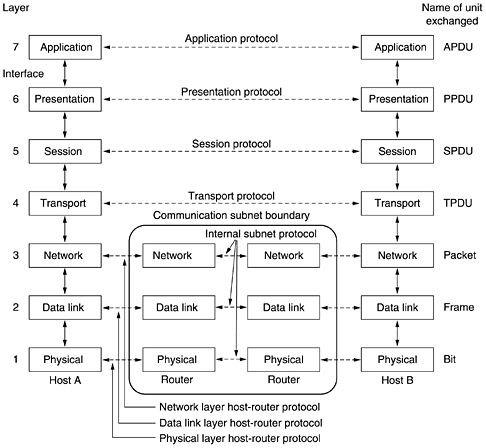
\includegraphics[width=\textwidth]{images/01fig20.png}
   \caption{The OSI Reference Model}
   \label{fig:osi-model}
\end{figure}


The OSI model has seven layers.
The principles that were applied to arrive at the seven layers can be briefly summarized as follows:

\begin{enumerate}
\item A layer should be created where a different abstraction is needed.
\item Each layer should perform a well-defined function.
\item The function of each layer should be chosen with an eye toward defining internationally standardized protocols.
\item The layer boundaries should be chosen to minimize the information flow across the interfaces.
\item The number of layers should be large enough that distinct functions need not be thrown together in the same layer out of necessity and small enough that the architecture does not become unwieldy.
\end{enumerate}

Below we will discuss each layer of the model in turn, starting at the
bottom layer. Note that the OSI model itself is not a network
architecture because it does not specify the exact services and
protocols to be used in each layer. It just tells what each layer should
do. However, ISO has also produced standards for all the layers,
although these are not part of the reference model itself. Each one has
been published as a separate international standard.

\subsubsection{The physical layer}

The \emph{physical layer} is concerned with transmitting raw bits over a communication channel.
The design issues have to do with making sure that when one side sends a 1 bit, it is received by the other side as a 1 bit, not as a 0 bit.
Typical questions here are how many volts should be used to represent a 1 and how many for a 0, how many nanoseconds a bit lasts, whether transmission may proceed simultaneously in both directions, how the initial connection is established and how it is torn down when both sides are finished, and how many pins the network connector has and what each pin is used for.
The design issues here largely deal with mechanical, electrical, and timing interfaces, and the physical transmission medium, which lies below the physical layer.


\subsubsection{The data link layer}

The main task of the \emph{data link layer} is to transform a raw transmission facility into a line that appears free of undetected
transmission errors to the network layer.
It accomplishes this task by having the sender break up the input data into \emph{data frames} (typically a few hundred or a few thousand bytes) and transmit the frames sequentially.
If the service is reliable, the receiver confirms correct receipt of each frame by sending back an \emph{acknowledgement frame}.

Another issue that arises in the data link layer (and most of the higher layers as well) is how to keep a fast transmitter from drowning a slow receiver in data.
Some traffic regulation mechanism is often needed to let the transmitter know how much buffer space the receiver has at the moment.
Frequently, this flow regulation and the error handling are integrated.

Broadcast networks have an additional issue in the data link layer: how to control access to the shared channel.
A special sublayer of the data link layer, the medium access control sublayer, deals with this problem.


\subsubsection{The network layer}

The \emph{network layer} controls the operation of the subnet.
A key design issue is determining how packets are routed from source to destination.
Routes can be based on static tables that are ``wired into'' the network and rarely changed.
They can also be determined at the start of each conversation, for example, a terminal session (e.g., a login to a remote
machine). Finally, they can be highly dynamic, being determined anew for
each packet, to reflect the current network load.

If too many packets are present in the subnet at the same time, they
will get in one another's way, forming bottlenecks. The control of such
congestion also belongs to the network layer. More generally, the
\emph{quality of service} provided (delay, transit time, jitter, etc.) is also a network layer issue.

When a packet has to travel from one network to another to get to its
destination, many problems can arise. The addressing used by the second
network may be different from the first one. The second one may not
accept the packet at all because it is too large. The protocols may
differ, and so on. It is up to the network layer to overcome all these
problems to allow heterogeneous networks to be interconnected.

In broadcast networks, the routing problem is simple, so the network
layer is often thin or even nonexistent.



\subsubsection{The transport layer}

The basic function of the \emph{transport layer} is to accept data from
above, split it up into smaller units if need be, pass these to the
network layer, and ensure that the pieces all arrive correctly at the
other end. Furthermore, all this must be done efficiently and in a way
that isolates the upper layers from the inevitable changes in the
hardware technology.

The transport layer also determines what type of service to provide to
the session layer, and, ultimately, to the users of the network. The
most popular type of transport connection is an error-free
point-to-point channel that delivers messages or bytes in the order in
which they were sent. However, other possible kinds of transport service
are the transporting of isolated messages, with no guarantee about the
order of delivery, and the broadcasting of messages to multiple
destinations. The type of service is determined when the connection is
established. (As an aside, an error-free channel is impossible to
achieve; what people really mean by this term is that the error rate is
low enough to ignore in practice.)

The transport layer is a true end-to-end layer, all the way from the
source to the destination. In other words, a program on the source
machine carries on a conversation with a similar program on the
destination machine, using the message headers and control messages. In
the lower layers, the protocols are between each machine and its
immediate neighbors, and not between the ultimate source and destination
machines, which may be separated by many routers. The difference between
layers 1 through 3, which are chained, and layers 4 through 7, which are
end-to-end, is illustrated in \vref{fig:osi-model}.


\subsubsection{The session layer}

The session layer allows users on different machines to establish
{sessions} between them. Sessions offer various services, including
{dialog control} (keeping track of whose turn it is to transmit), {token
management} (preventing two parties from attempting the same critical
operation at the same time), and {synchronization} (checkpointing long
transmissions to allow them to continue from where they were after a
crash).


\subsubsection{The presentation layer}

Unlike lower layers, which are mostly concerned with moving bits around,
the {presentation layer} is concerned with the syntax and semantics of
the information transmitted. In order to make it possible for computers
with different data representations to communicate, the data structures
to be exchanged can be defined in an abstract way, along with a standard
encoding to be used ``on the wire.''
The presentation layer manages these abstract data structures and allows higher-level data structures (e.g., banking records), to be defined and exchanged.


\subsubsection{The application layer}

The \emph{application layer} contains a variety of protocols that are
commonly needed by users. One widely-used application protocol is {HTTP}
({HyperText Transfer Protocol}), which is the basis for the World Wide
Web. When a browser wants a Web page, it sends the name of the page it
wants to the server using HTTP. The server then sends the page back.
Other application protocols are used for file transfer, electronic mail,
and network news.



\subsection{The TCP/IP Reference Model}

Let us now turn from the OSI reference model to the reference model used
in the grandparent of all wide area computer networks, the ARPANET, and
its successor, the worldwide Internet. Although we will give a brief
history of the ARPANET later, it is useful to mention a few key aspects
of it now. The ARPANET was a research network sponsored by the DoD (U.S.
Department of Defense). It eventually connected hundreds of universities
and government installations, using leased telephone lines. When
satellite and radio networks were added later, the existing protocols
had trouble interworking with them, so a new reference architecture was
needed. Thus, the ability to connect multiple networks in a seamless way
was one of the major design goals from the very beginning. This
architecture later became known as the {TCP/IP Reference Model}, after
its two primary protocols. It was first defined in (Cerf and Kahn,
1974). A later perspective is given in (Leiner et al., 1985). The design
philosophy behind the model is discussed in (Clark, 1988).

Given the DoD's worry that some of its precious hosts, routers, and
internetwork gateways might get blown to pieces at a moment's notice,
another major goal was that the network be able to survive loss of
subnet hardware, with existing conversations not being broken off. In
other words, DoD wanted connections to remain intact as long as the
source and destination machines were functioning, even if some of the
machines or transmission lines in between were suddenly put out of
operation. Furthermore, a flexible architecture was needed since
applications with divergent requirements were envisioned, ranging from
transferring files to real-time speech transmission.


\subsubsection{The internet layer}

All these requirements led to the choice of a packet-switching network
based on a connectionless internetwork layer. This layer, called the
\emph{internet layer}, is the linchpin that holds the whole architecture
together. Its job is to permit hosts to inject packets into any network
and have them travel independently to the destination (potentially on a
different network). They may even arrive in a different order than they
were sent, in which case it is the job of higher layers to rearrange
them, if in-order delivery is desired. Note that ``internet'' is used
here in a generic sense, even though this layer is present in the
Internet.

The analogy here is with the (snail) mail system. A person can drop a
sequence of international letters into a mail box in one country, and
with a little luck, most of them will be delivered to the correct
address in the destination country. Probably the letters will travel
through one or more international mail gateways along the way, but this
is transparent to the users. Furthermore, that each country (i.e., each
network) has its own stamps, preferred envelope sizes, and delivery
rules is hidden from the users.

The internet layer defines an official packet format and protocol called
{IP} ({Internet Protocol}). The job of the internet layer is to deliver
IP packets where they are supposed to go. Packet routing is clearly the
major issue here, as is avoiding congestion. For these reasons, it is
reasonable to say that the TCP/IP internet layer is similar in
functionality to the OSI network layer.
\Cref{fig:tcpip-model} shows this correspondence.


\begin{figure}
   \centering
   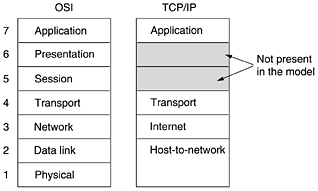
\includegraphics[width=.8\textwidth]{images/01fig21.png}
   \caption{The TCP/IP reference model}
   \label{fig:tcpip-model}
\end{figure}


\subsubsection{The transport layer}

The layer above the internet layer in the TCP/IP model is now usually
called the {transport layer}. It is designed to allow peer entities on
the source and destination hosts to carry on a conversation, just as in
the OSI transport layer. Two end-to-end transport protocols have been
defined here. The first one, {TCP} ({Transmission Control Protocol}), is
a reliable connection-oriented protocol that allows a byte stream
originating on one machine to be delivered without error on any other
machine in the internet. It fragments the incoming byte stream into
discrete messages and passes each one on to the internet layer. At the
destination, the receiving TCP process reassembles the received messages
into the output stream. TCP also handles flow control to make sure a
fast sender cannot swamp a slow receiver with more messages than it can
handle.

The second protocol in this layer, {UDP} ({User Datagram Protocol}), is
an unreliable, connectionless protocol for applications that do not want
TCP's sequencing or flow control and wish to provide their own. It is
also widely used for one-shot, client-server-type request-reply queries
and applications in which prompt delivery is more important than
accurate delivery, such as transmitting speech or video. The relation of
IP, TCP, and UDP is shown in \cref{fig:tcpip-model-protocols}.
Since the model was developed, IP has been implemented on many other networks.



\begin{figure}
   \centering
   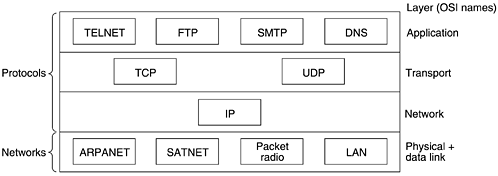
\includegraphics[width=\textwidth]{images/01fig22.png}
   \caption{Protocols and networks in the TCP/IP model initially}
   \label{fig:tcpip-model-protocols}
\end{figure}



\subsubsection{The application layer}

The TCP/IP model does not have session or presentation layers. No need
for them was perceived, so they were not included. Experience with the
OSI model has proven this view correct: they are of little use to most
applications.

On top of the transport layer is the \emph{application layer}.
It contains all the higher-level protocols.
The early ones included virtual terminal (TELNET), file transfer (FTP), and electronic mail (SMTP), as shown in \cref{fig:tcpip-model-protocols}.
The virtual terminal protocol allows a user on one machine to log onto a distant machine and work there.
The file transfer protocol provides a way to move data efficiently from one machine to another.
Electronic mail was originally just a kind of file transfer, but later a specialized protocol (SMTP) was developed for it.
Many other protocols have been added to these over the years: the Domain Name System (DNS) for mapping host names onto their network addresses, NNTP, the protocol for moving USENET news articles around, and HTTP, the protocol for fetching pages on the World Wide Web, and many others.


\subsubsection{The host-to-network layer}

Below the internet layer is a great void. The TCP/IP reference model
does not really say much about what happens here, except to point out
that the host has to connect to the network using some protocol so it
can send IP packets to it. This protocol is not defined and varies from
host to host and network to network. Books and papers about the TCP/IP
model rarely discuss it.



\subsection{A comparison of the OSI and TCP/IP reference models}

The OSI and TCP/IP reference models have much in common. Both are based
on the concept of a stack of independent protocols. Also, the
functionality of the layers is roughly similar. For example, in both
models the layers up through and including the transport layer are there
to provide an end-to-end, network-independent transport service to
processes wishing to communicate. These layers form the transport
provider. Again in both models, the layers above transport are
application-oriented users of the transport service.

Despite these fundamental similarities, the two models also have many
differences. In this section we will focus on the key differences
between the two reference models. It is important to note that we are
comparing the {reference models} here, not the corresponding {protocol
stacks}. The protocols themselves will be discussed later. For an entire
book comparing and contrasting TCP/IP and OSI, see (Piscitello and
Chapin, 1993).

Three concepts are central to the OSI model:
\begin{enumerate}
\item services,
\item interfaces, and
\item protocols.
\end{enumerate}

Probably the biggest contribution of the OSI model is to make the distinction between these three concepts explicit.
Each layer performs some services for the layer above it. The {service} definition tells what the layer does, not how entities above it access it or how the
layer works. It defines the layer's semantics.

A layer's {interface} tells the processes above it how to access it. It
specifies what the parameters are and what results to expect. It, too,
says nothing about how the layer works inside.

Finally, the peer {protocols} used in a layer are the layer's own
business. It can use any protocols it wants to, as long as it gets the
job done (i.e., provides the offered services). It can also change them
at will without affecting software in higher layers.

These ideas fit very nicely with modern ideas about object-oriented
programming. An object, like a layer, has a set of methods (operations)
that processes outside the object can invoke. The semantics of these
methods define the set of services that the object offers. The methods'
parameters and results form the object's interface. The code internal to
the object is its protocol and is not visible or of any concern outside
the object.

The TCP/IP model did not originally clearly distinguish between service,
interface, and protocol, although people have tried to retrofit it after
the fact to make it more OSI-like. For example, the only real services
offered by the internet layer are SEND IP PACKET and RECEIVE IP PACKET.

As a consequence, the protocols in the OSI model are better hidden than
in the TCP/IP model and can be replaced relatively easily as the
technology changes. Being able to make such changes is one of the main
purposes of having layered protocols in the first place.

The OSI reference model was devised {before} the corresponding protocols
were invented. This ordering means that the model was not biased toward
one particular set of protocols, a fact that made it quite general. The
downside of this ordering is that the designers did not have much
experience with the subject and did not have a good idea of which
functionality to put in which layer.

For example, the data link layer originally dealt only with
point-to-point networks. When broadcast networks came around, a new
sublayer had to be hacked into the model. When people started to build
real networks using the OSI model and existing protocols, it was
discovered that these networks did not match the required service
specifications (wonder of wonders), so convergence sublayers had to be
grafted onto the model to provide a place for papering over the
differences. Finally, the committee originally expected that each
country would have one network, run by the government and using the OSI
protocols, so no thought was given to internetworking. To make a long
story short, things did not turn out that way.

With TCP/IP the reverse was true: the protocols came first, and the
model was really just a description of the existing protocols. There was
no problem with the protocols fitting the model. They fit perfectly. The
only trouble was that the {model} did not fit any other protocol stacks.
Consequently, it was not especially useful for describing other,
non-TCP/IP networks.

Turning from philosophical matters to more specific ones, an obvious
difference between the two models is the number of layers: the OSI model
has seven layers and the TCP/IP has four layers. Both have
(inter)network, transport, and application layers, but the other layers
are different.

Another difference is in the area of connectionless versus
connection-oriented communication. The OSI model supports both
connectionless and connection-oriented communication in the network
layer, but only connection-oriented communication in the transport
layer, where it counts (because the transport service is visible to the
users). The TCP/IP model has only one mode in the network layer
(connectionless) but supports both modes in the transport layer, giving
the users a choice. This choice is especially important for simple
request-response protocols.


\subsection{A Critique of the OSI Model and Protocols}

Neither the OSI model and its protocols nor the TCP/IP model and its
protocols are perfect. Quite a bit of criticism can be, and has been,
directed at both of them. In this section and the next one, we will look
at some of these criticisms. We will begin with OSI and examine TCP/IP
afterward.

At the time the second edition of this book was published (1989), it
appeared to many experts in the field that the OSI model and its
protocols were going to take over the world and push everything else out
of their way. This did not happen. Why? A look back at some of the
lessons may be useful. These lessons can be summarized as:

\begin{enumerate}
\item Bad timing.
\item Bad technology.
\item Bad implementations.
\item Bad politics.
\end{enumerate}


\subsubsection{Bad timing}

First let us look at reason one: bad timing. The time at which a standard is established is absolutely critical to its success.
David Clark of MIT\ has a theory of standards that he calls the {apocalypse of the two elephants}, which is illustrated in \cref{fig:two-elephants}.

\begin{figure}
   \centering
   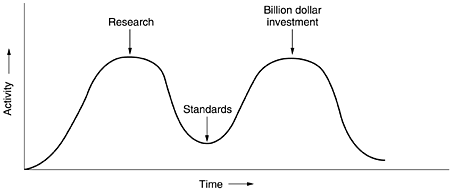
\includegraphics[width=\textwidth]{images/01fig23.png}
   \caption{The apocalypse of the two elephants}
   \label{fig:two-elephants}
\end{figure}


This figure shows the amount of activity surrounding a new subject. When
the subject is first discovered, there is a burst of research activity
in the form of discussions, papers, and meetings. After a while this
activity subsides, corporations discover the subject, and the
billion-dollar wave of investment hits.

It is essential that the standards be written in the trough in between
the two ``elephants.''
If the standards are written too early, before
the research is finished, the subject may still be poorly understood;
the result is bad standards. If they are written too late, so many
companies may have already made major investments in different ways of
doing things that the standards are effectively ignored. If the interval
between the two elephants is very short (because everyone is in a hurry
to get started), the people developing the standards may get crushed.

It now appears that the standard OSI protocols got crushed. The
competing TCP/IP protocols were already in widespread use by research
universities by the time the OSI protocols appeared. While the
billion-dollar wave of investment had not yet hit, the academic market
was large enough that many vendors had begun cautiously offering TCP/IP
products. When OSI came around, they did not want to support a second
protocol stack until they were forced to, so there were no initial
offerings. With every company waiting for every other company to go
first, no company went first and OSI never happened.


\subsubsection{Bad technology}

The second reason that OSI never caught on is that both the model and
the protocols are flawed. The choice of seven layers was more political
than technical, and two of the layers (session and presentation) are
nearly empty, whereas two other ones (data link and network) are
overfull.

The OSI model, along with the associated service definitions and protocols, is extraordinarily complex.
When piled up, the printed standards occupy a significant fraction of a meter of paper.
They are also difficult to implement and inefficient in operation.
In this context, a riddle posed by Paul Mockapetris and cited in (Rose, 1993) comes to mind:

\begin{quote}
   \textbf{Question:}
   What do you get when you cross a mobster with an international standard?\\
   \textbf{Answer:}
   Someone who makes you an offer you can't understand.
\end{quote}

In addition to being incomprehensible, another problem with OSI is that
some functions, such as addressing, flow control, and error control,
reappear again and again in each layer. Saltzer et al. (1984), for
example, have pointed out that to be effective, error control must be
done in the highest layer, so that repeating it over and over in each of
the lower layers is often unnecessary and inefficient.



\subsubsection{Bad implementations}

Given the enormous complexity of the model and the protocols, it will
come as no surprise that the initial implementations were huge,
unwieldy, and slow. Everyone who tried them got burned. It did not take
long for people to associate ``OSI'' with ``poor quality.''
Although the products improved in the course of time, the image stuck.

In contrast, one of the first implementations of TCP/IP was part of
Berkeley UNIX and was quite good (not to mention, free). People began
using it quickly, which led to a large user community, which led to
improvements, which led to an even larger community. Here the spiral was
upward instead of downward.


\subsubsection{Bad politics}

On account of the initial implementation, many people, especially in
academia, thought of TCP/IP as part of UNIX, and UNIX in the 1980s in
academia was not unlike parenthood (then incorrectly called motherhood)
and apple pie.

OSI, on the other hand, was widely thought to be the creature of the
European telecommunication ministries, the European Community, and later
the U.S. Government. This belief was only partly true, but the very idea
of a bunch of government bureaucrats trying to shove a technically
inferior standard down the throats of the poor researchers and
programmers down in the trenches actually developing computer networks
did not help much. Some people viewed this development in the same light
as IBM announcing in the 1960s that PL/I was the language of the future,
or DoD correcting this later by announcing that it was actually Ada.



\subsection{A critique of the TCP/IP reference model}

The TCP/IP model and protocols have their problems too.
First, the model does not clearly distinguish the concepts of service, interface, and
protocol. Good software engineering practice requires differentiating
between the specification and the implementation, something that OSI
does very carefully, and TCP/IP does not. Consequently, the TCP/IP model
is not much of a guide for designing new networks using new
technologies.

Second, the TCP/IP model is not at all general and is poorly suited to
describing any protocol stack other than TCP/IP. Trying to use the
TCP/IP model to describe Bluetooth, for example, is completely
impossible.

Third, the host-to-network layer is not really a layer at all in the
normal sense of the term as used in the context of layered protocols. It
is an interface (between the network and data link layers). The
distinction between an interface and a layer is crucial, and one should
not be sloppy about it.

Fourth, the TCP/IP model does not distinguish (or even mention) the
physical and data link layers. These are completely different. The
physical layer has to do with the transmission characteristics of copper
wire, fiber optics, and wireless communication. The data link layer's
job is to delimit the start and end of frames and get them from one side
to the other with the desired degree of reliability. A proper model
should include both as separate layers. The TCP/IP model does not do
this.

Finally, although the IP and TCP protocols were carefully thought out
and well implemented, many of the other protocols were ad hoc, generally
produced by a couple of graduate students hacking away until they got
tired. The protocol implementations were then distributed free, which
resulted in their becoming widely used, deeply entrenched, and thus hard
to replace. Some of them are a bit of an embarrassment now. The virtual
terminal protocol, TELNET, for example, was designed for a ten-character
per second mechanical Teletype terminal. It knows nothing of graphical
user interfaces and mice. Nevertheless, 25 years later, it is still in
widespread use.

In summary, despite its problems, the OSI {model} (minus the session and
presentation layers) has proven to be exceptionally useful for
discussing computer networks. In contrast, the OSI {protocols} have not
become popular. The reverse is true of TCP/IP: the {model} is
practically nonexistent, but the {protocols} are widely used. Since
computer scientists like to have their cake and eat it, too, in this
book we will use a modified OSI model but concentrate primarily on the
TCP/IP and related protocols, as well as newer ones such as 802, SONET,
and Bluetooth.
In effect, we will use the hybrid model of \cref{fig:hybrid-model}.


\begin{figure}
   \centering
   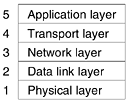
\includegraphics[width=.2\textwidth]{images/01fig24.png}
   \caption{The hybrid reference model to be used in this book.}
   \label{fig:hybrid-model}
\end{figure}



\part{IP addressing}

% Kozierok, ch. 15
\chapter{Internet Protocol versions, concepts, and overview}


The Internet Protocol (IP) is a very important protocol in
internetworking. It would be no exaggeration to say that you can't
really comprehend modern networking without a good understanding of IP.
Unfortunately, IP can be somewhat difficult to understand. A large
amount of complexity has become associated with it over the years, and
this has allowed it to meet the many demands placed on it.

Before diving into the details of how IP works, we'll look at the basic
concepts underlying IP. In this chapter, I explain how IP operates in
basic terms and the most important aspects of how it does its job. We'll
look at its main functions, its history, and how it has spawned the
development of several IP-related protocols.



\section{IP overview and key operational characteristics}

IP is the core of the TCP/IP protocol suite and the main protocol at the network layer.
The network layer is primarily concerned with the delivery of data between devices that may be on different networks, which are
interconnected in an arbitrary manner.
In other words, an {\emph{internetwork}}.
IP is the mechanism by which this data is sent on TCP/IP networks (with help from other protocols at the network layer, too, of course).

Let's look at the TCP/IP layer model and consider what IP does from an
architectural standpoint. As the layer~3 protocol, it provides a service
to layer~4 in the TCP/IP stack, represented mainly by the Transmission
Control Protocol (TCP) and User Datagram Protocol (UDP) (see
\protect\hyperlink{pt11.html}{Part~II-8}).
IP takes data that has been packaged by either TCP or UDP, manipulates it as necessary, and sends it out (see \cref{fig:ip-main-function}).

This service is sometimes called {\emph{internetwork datagram delivery}}.
There are many details that explain exactly how this service is accomplished, but in a nutshell, IP sends data from point A to point B over an internetwork of connected networks.


\begin{figure}
   \centering
   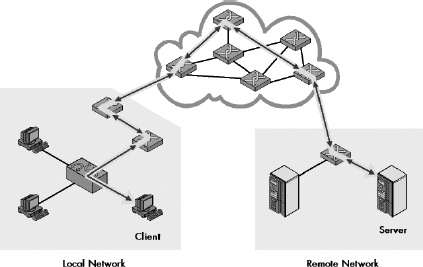
\includegraphics[width=.7\textwidth]{images/ip-main-function.jpg}
   \caption{The main function of IP: internetwork datagram delivery -- IP's overall responsibility is to deliver data between devices on unconnected networks. This figure shows how IP delivers datagrams from one device to another over an internetwork; in this case, a distant client and server communicate with each other by passing IP datagrams over a series of interconnected networks.}
   \label{fig:ip-main-function}
\end{figure}



{\textbf{KEY CONCEPT}} While the {\emph{Internet Protocol}} has many
functions and characteristics, it can be boiled down to one primary
purpose: the delivery of datagrams across an internetwork of connected
networks.\protect\hypertarget{ch15.htmlux5cux23idx-CHP-15-0638}{}{}

Of course, there are many ways in which IP could have been implemented in order to accomplish this task.
To understand how the designers of TCP/IP made IP work, let's take a look at the key characteristics used to describe IP and the general manner in which it operates:

\begin{description}
   \item[Universally addressed]
      In order to send data from point A to point B, it is necessary to ensure that devices know how to identify which device is point B.
      IP defines the addressing mechanism for the network and uses these addresses for delivery purposes.

   \item[Underlying protocol-independent]
      IP is designed to allow the transmission of data across any type of underlying network that is designed to work with a TCP/IP stack.
      It includes provisions that allow it to adapt to the requirements of various lower-level protocols such as Ethernet or IEEE 802.11.
      IP can also run on the special data link protocols, Serial Line Interface Protocol (SLIP) and Point-to-Point Protocol (PPP), that were created for it (see \protect\hyperlink{pt04.html}{Part~II-1}).
      An important example is IP's ability to fragment large blocks of data into smaller ones in order to match the size limitations of physical networks, and then have the recipient reassemble the pieces again as needed.

   \item[Connectionless delivery]
      IP is a {\emph{connectionless protocol}}.
      This means that when point A wants to send data to point B, it doesn't first set up a connection to point B and then send the data -- it just makes the datagram and sends it.
      (See the section in \protect\hyperlink{ch01.html}{Chapter~1} on connection-oriented and connectionless protocols for more information on this.)

   \item[Unreliable delivery]
      IP is said to be an unreliable protocol.
      That doesn't mean that one day your IP software will decide to go fishing rather than run your network.
      It does mean that when datagrams are sent from Device A to Device B, Device A just sends each one and then moves on to the next.
      IP doesn't keep track of the ones it sent.
      It does not provide reliability or service-quality capabilities, such as error protection for the data it sends (though it does on the IP header), flow control, or retransmission of lost datagrams.
      For this reason, IP is sometimes called a {\emph{best-effort}} protocol.
      It does what it can to get data to where it needs to go, but makes no guarantees that the data will actually get there.

   \item[Unacknowledged delivery]
      Corresponding with its unreliable nature, IP doesn't use acknowledgements.
      When Device B gets a datagram from Device A, it doesn't send back a "thank you note" to tell Device A that the datagram was received.
      It leaves Device A in the dark, so to speak.
\end{description}

These last three characteristics might be enough to make you cringe,
thinking that giving your data to IP would be somewhat like trusting a
new car to your 16-year-old son. If you are going to build an entire
network around this protocol, why design it so that it works without
connections, doesn't guarantee that the data will get there, and has no
means of acknowledging receipt of data?

The reason is simple: Establishing connections, guaranteeing delivery,
error checking, and similar insurance-type
\protect\hypertarget{ch15.htmlux5cux23idx-CHP-15-0640}{}{}functions have
a cost in {\emph{performance}}. It takes time, computer resources, and
network bandwidth to perform these tasks, and they aren't always
necessary for every application. Now, consider that IP carries pretty
much {\emph{all}} user traffic on a TCP/IP network. To build this
complexity into IP would burden all traffic with this overhead, whether
or not it was needed.

The solution taken by the designers of TCP/IP was to exploit the power
of layering. If service-quality features such as connections, error
checking, or guaranteed delivery are required by an application, they
are provided at the transport layer (or possibly, the application
layer). On the other hand, applications that don't need these features
can avoid using them. This is the major distinction between the two
TCP/IP transport layer protocols: TCP and UDP. TCP is full featured but
a bit slower than UDP; UDP is spartan in its capabilities, but faster
than TCP. This system is really the best of both worlds, and it works.



\section{IP functions}

The exact number of IP functions depends on where you draw the line between certain activities.
For explanatory purposes, however, I view IP as having four basic functions (or more accurately, function sets):
\begin{description}
   \item[Addressing]
      Before it can deliver datagrams, IP must know where to deliver them.
      For this reason, IP includes a mechanism for host addressing.
      Furthermore, since IP operates over internetworks, its system is designed to allow for the unique addressing of devices across arbitrarily large networks.
      It also contains a structure to facilitate the routing of datagrams to distant networks, if that is required.
      Since most of the other TCP/IP protocols use IP, an understanding the IP addressing scheme is of vital importance to comprehending much of what goes on in TCP/IP.
      It is explored fully in Chapters \vref{chap:kozierok-ch16} through \vref{chap:kozierok-ch20}.

   \item[Data encapsulation and formatting/packaging]
      As the TCP/IP network layer protocol, IP accepts data from the transport layer protocols UDP and TCP.
      It then encapsulates this data into an IP datagram using a special format prior to transmission.

   \item[Fragmentation and reassembly]
      IP datagrams are passed down to the data link layer for transmission on the local network.
      However, the maximum frame size of each physical and data link network using IP may be different.
      For this reason, IP includes the ability to {\emph{fragment}} IP datagrams into pieces, so that they can each be carried on the local network.
      The receiving device uses the {\emph{reassembly}} function to re-create the whole IP datagram.
      Some people view fragmentation and reassembly as distinct functions, though clearly they are complementary, and I view them as being part of the same job.

   \item[Routing and indirect delivery]
      When an IP datagram must be sent to a destination on the same local network, you can do this easily with the network's underlying local area network (LAN), wireless LAN (WLAN), or wide area network (WAN) protocol, using what is sometimes called {\emph{direct delivery}}.
      However, in many (if not most cases) the final destination is on a distant network that isn't directly attached to the source.
      In this situation, the datagram must be delivered indirectly.
      This is accomplished by routing the datagram through intermediate devices ({\emph{routers}}).
      \protect\hypertarget{ch15s02.htmlux5cux23idx-CHP-15-0641}{}{}IP accomplishes this in concert with support from the other protocols including the Internet Control Message Protocol (ICMP) and the TCP/IP gateway/routing protocols such as the Routing Information Protocol (RIP) and the Border Gateway Protocol (BGP).
\end{description}


\section{IP history, standards, versions, and closely related protocols}

Since IP is really the architectural foundation for the entire TCP/IP
protocol suite, you might have expected that it was created first, and
that the other protocols were built upon it. That's usually how you
build a structure, after all! The history of IP, however, is a bit more
complex. The functions it {\emph{performs}} were defined at the birth of
the protocol, but IP itself didn't exist for the first few years that
the protocol suite was being
defined.\protect\hypertarget{ch15s03.htmlux5cux23idx-CHP-15-0643}{}{}\protect\hypertarget{ch15s03.htmlux5cux23idx-CHP-15-0644}{}{}\protect\hypertarget{ch15s03.htmlux5cux23idx-CHP-15-0645}{}{}

I explore the early days of TCP/IP in \protect\hyperlink{ch08.html}{Chapter~8}, which provides an overview of the suite as a whole.
What is notable about the development of IP is that its functions were originally part of TCP.
As a formal protocol, IP was born when an early version of TCP developed in the 1970s for predecessors of the modern Internet was split into TCP at layer~4 and IP at layer~3.
The key milestone in the development of IP was the publication of RFC 791, ``Internet Protocol,'' in September 1981.
This standard, a revision of the similar RFC 760 of the previous year, defined the core functionality and characteristics of the version of IP that has been in widespread use for the last two decades.



\subsection{IP versions and version numbers}

The IP defined in RFC 791 was the first widely used version of IP.
Interestingly, however, it is not version 1 of IP but version 4! This would of course imply that there were earlier versions of the protocol at one point.
Interestingly, however, there really weren't.
IP was created when its functions were split out from an early version of TCP that combined both TCP and IP functions.
TCP evolved through three earlier versions and was split into TCP and IP for version 4.
That version number was applied to both TCP and IP for consistency.


{\textbf{KEY CONCEPT}} Version 4 of the {\emph{Internet Protocol}} (IP)
is actually the first version that was widely deployed and is currently
the one in widespread use.

So, when you use IP today, you are using IP version 4, which is
frequently abbreviated IPv4. Unless otherwise qualified, it's safe to
assume that {\emph{IP}} means IP version 4 -- at least for the next few years.
(This version number is carried in the appropriate field of all IP datagrams, as described in the topic discussing the IP datagram format in \vref{chap:kozierok-ch21}.)

Given that it was originally designed for an internetwork a tiny
fraction of the size of our current Internet, IPv4 has proven itself remarkably capable.
Various additions and changes have been made over
time to how IP is used, especially with respect to addressing, but the
core protocol is basically what it was in the early 1980s. There's good
reason for this. Changing something as fundamental as IP requires a
great deal of development effort and also introduces complexities during
transition.

IPv4 has served us well, but people understood that, for various
reasons, a new version of IP would eventually be required. Due to the
difficulties associated with making such an important change,
development of this new version of IP has actually been under way since
the mid-1990s. This new version of IP is formally called {\emph{Internet
Protocol version 6 (IPv6)}} and also sometimes referred to as {\emph{IP
Next Generation}} or {\emph{IPng}}. I discuss the reasons why IPv6 was
developed and how it differs from IPv4 in considerable detail in
\protect\hyperlink{pt07.html}{Part~II-4} of this book.

A natural question at this point is, "What happened to version 5 of IP?"
The answer is that it doesn't exist. While this may seem confusing,
version 5 was in fact intentionally skipped in order to {\emph{avoid}}
confusion, or at least to rectify it. The problem with version 5 relates
to an experimental TCP/IP protocol called the {\emph{Internet Stream
Protocol, version 2}}, originally defined in RFC 1190. This protocol was
originally seen by some as being a peer of IP at the Internet layer in
the TCP/IP architecture, and in its standard version, these packets were
assigned IP version 5 to differentiate them from normal IP packets
(version 4). This protocol apparently never went anywhere, but to be
absolutely sure that there would be no confusion, version 5 was skipped
over in favor of version 6.




\subsection{IP-related protocols}


In addition to the old and new versions of IP, there are several protocols that are {\emph{IP-related}}.
These are protocols that add to or expand on the capabilities of IP functions for special circumstances, but they are not part of IP proper.
These are as follows:
\begin{description}
   \item[Network address translation]
      This protocol\footnote{NAT is not a protocol. Kozierok is wrong here.} provides IP address translation capabilities that allow private networks to be interfaced to public networks in a flexible manner.
      It allows public IP addresses to be shared and improves security by making it more difficult for hosts on the public network to gain unauthorized access to hosts.
      It is commonly called {\emph{NAT}}.
      This protocol is discussed in \vref{chap:nat}.

   \item[IPsec]
      IPsec defines a set of subprotocols that provide a mechanism for the secure transfer of data using IP.
      It is rapidly growing in popularity as a security protocol that enables virtual private networks.
      This protocol\footnote{IPsec can better be described as a set of protocols or a framework.} is discussed in \protect\hyperlink{ch29.html}{Chapter~29}.

   \item[Mobile IP]
      This is a protocol that addresses some of the difficulties associated with using IP on computers that frequently move from one network to another.
      It provides a mechanism that allows data to be automatically routed to a mobile host (such as a notebook computer), without requiring a constant reconfiguration of the device's IP address.
      This protocol is discussed in \protect\hyperlink{ch30.html}{Chapter~30}.
\end{description}





% Kozierok, ch. 16
\chapter{IPv4 addressing concepts and issues}
\label{chap:kozierok-ch16}

The primary job of the Internet Protocol (IP) is delivering messages
between devices, and like any good delivery service, it can't do its job
too well if it doesn't know where the recipients are located. Obviously
then, one of the most important functions of IP is {\emph{addressing}}.
IP addressing is used not only to uniquely identify IP addresses, but
also to facilitate the routing of IP datagrams over internetworks. IP
addresses are used and referred to extensively in TCP/IP networking.

Even though the original IP addressing scheme was relatively simple, it
has become complex over time as changes have been made to it to allow it
to deal with various addressing requirements. The more advanced styles
of IP addressing, such as subnetting and classless addressing, are the
ones used most in modern networks. However, they can be a bit confusing
to understand. To help make sense of them, we must start at the
beginning with a discussion of the fundamentals of IP addressing.

In this chapter, I begin a larger exploration of
\protect\hypertarget{ch16.htmlux5cux23idx-CHP-16-0646}{}{}IP addressing
by explaining the key concepts and issues behind it. I begin with an
overview of IP addressing and a discussion of what it is all about. I
describe the size of IP addresses, the concept of its address space, and
the notation usually used for IP addresses. I provide basic information
on the structure of an IP address and how it is divided into a network
identifier and host identifier. I then describe the different types of
IP addresses and the additional information, such as a subnet mask and
default gateway, that often accompanies an IP address on larger
networks. I provide a brief description of how multiple addresses are
sometimes assigned to single devices and why. I conclude with a
description of the process by which public IP addresses are registered
and managed, and the organizations that do this work for the global
Internet.

{\textbf{BACKGROUND INFORMATION}} {\emph{If you are not familiar with at
least the basics of how binary numbers work, and also with how to
convert between binary and decimal numbers, I recommend reading
\protect\hyperlink{ch04.html}{Chapter~4}, which provides some background
on data representation and the mathematics of computing, before you
proceed here}}.




\section{IP addressing overview and fundamentals}


IP addressing is important because it facilitates the primary function
of the IP: the delivery of datagrams across an internetwork. When you
examine this in more detail, it becomes apparent that the IP address
actually has two different functions, as follows:
\begin{description}
   \item[Network interface identification]
      Like a street address, the IP address provides unique identification of the interface between a device and the network.
      This is required to ensure that the datagram is delivered to the correct recipients.
   \item[Routing]
      When the source and destination of an IP datagram are not on the same network, the datagram must be delivered indirectly using intermediate systems.
      This is a process called \emph{routing}.
      The IP address is an essential part of the system used to route datagrams.
\end{description}

You may have noticed a couple of things about this short list.
One is
that I said the IP address identifies the {\emph{network interface}},
not that it identifies the {\emph{device}} itself. This distinction is
important because it underscores the concept that IP is oriented around
connections to a large, virtual network at layer~3, which can span
multiple physical networks. Some devices, such as routers, will have
more than one network connection, necessary to take datagrams from one
network and route them onto another. This means they will also have more
than one IP address -- one per connection.

You might also find it curious that I said that the IP address
facilitates routing. How can it do that? The answer is that the
addressing system is designed with a structure that can be interpreted
to allow routers to determine what to do with a datagram based on the
values in the address. Numbers related to the IP address, such as the
subnet mask when subnetting is used, support this function.

Let's look at some of the more important issues and characteristics
associated with IP addresses in general terms.

\subsection{Number of IP addresses per device}

Any device that has data sent to it at the network layer will have at
least one IP address: one per network interface. This means that normal
hosts such as computers and network-capable printers usually get one IP
address, while routers get more than one IP address. Some special hosts
may have more than one IP address if they are multihomed -- connected to
more than one network.

Lower-level network interconnection devices -- such as repeaters,
bridges, and switches -- don't require an IP address because they pass
traffic based on layer~2 (data link layer) addresses. Network segments
connected by bridges and switches form a single broadcast domain, and
any devices on them can send data to each other directly without
routing. To IP, these devices are essentially invisible; they are no
more significant than the wires that connect devices together (with a
couple of exceptions). Such devices may, however, optionally have an IP
address for management purposes. In this regard, they are acting like a
regular host on the network.

\Cref{fig:ip-interfaces} shows the IP interfaces of a few common LAN devices as small circles.
Each regular host has one interface, while the router that serves this LAN has three, since it connects to three different networks.
Note that the LAN switch has no IP interfaces; it connects the hosts and router at layer~2.
(Also see \protect\hyperlink{ch16s06.htmlux5cux23multihomed_devices_on_an_ip_internetwork}{Figure~16-5}, which shows the IP interfaces of devices in a more complex configuration.)


\begin{figure}
   \centering
   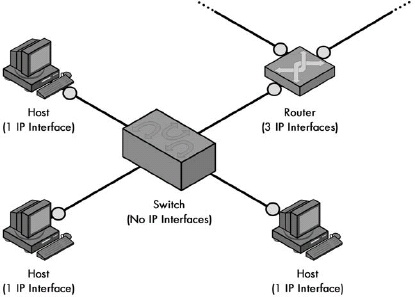
\includegraphics[width=.6\textwidth]{images/ip-interfaces.jpg}
   \caption{IP interfaces for common network devices -- Regular hosts have one interface; routers usually have more than one; and switches have none (because they operate at layer~2).}
   \label{fig:ip-interfaces}
\end{figure}



\subsection{Address uniqueness and network specificity}

Each IP address on a single internetwork must be unique.
(This seems rather obvious, although there are exceptions in IPv6, in the form of special anycast addresses, as discussed in \protect\hyperlink{ch25.html}{Chapter~25}.)

Since IP addresses represent network interfaces and are used for routing, the IP address is
specific to the network to which it is connected. If the device moves to
a new network, the IP address will usually have to change as well. For
the full reason why, see the discussion of basic IP address structure
later in this chapter. This issue was a primary motivation for the
creation of Mobile IP (covered in
\protect\hyperlink{ch30.html}{Chapter~30}).



\subsection{Contrasting IP addresses and data link layer addresses}

\protect\hypertarget{ch16.htmlux5cux23idx-CHP-16-0648}{}{}IP addresses
are used for network-layer data delivery across an internetwork. This
makes IP addresses quite different from the data link layer address of a
device, such as its Ethernet MAC address. (In TCP/IP parlance, these are
sometimes called {\emph{physical addresses}} or
\protect\hypertarget{ch16.htmlux5cux23idx-CHP-16-0649}{}{}{\emph{hardware
addresses}}.)

At the network layer, a single datagram may be sent from device~A to device~B.
However, the actual delivery of the datagram may require that it passes through a dozen or more physical devices if device~A and device~B are not on the same network.

It is also necessary to provide a function that maps between IP and data link layer addresses.
In TCP/IP, this is the job of the Address Resolution Protocol (ARP; see \protect\hyperlink{ch13.html}{Chapter~13}).

In a physical network such as an Ethernet, the MAC address is all the
information needed to send data between devices. In contrast, an IP
address represents only the final delivery point of the datagram. The
route taken depends on the characteristics of the network paths between
the source and destination devices. It is even possible that there may
not be a route between any two devices, which means two devices cannot
exchange data, even if they know each other's addresses!



\subsection{Private and public IP network addresses}

There are two distinct ways that a network can be set up with IP addresses.
On a {\emph{private network}}, a single organization controls the assignment of the addresses for all devices; they have pretty much absolute control to do what they wish in selecting numbers, as long as each address is unique.

In contrast, on a {\emph{public network}}, a mechanism is required to ensure that organizations don't use overlapping addresses and that they enable efficient routing of data between organizations.
The best-known example of this is the Internet, where public IP registration and management facilities have been created to address this issue.
There are also advanced techniques now, such as IP network address translation (NAT), which allow a network using private addresses to be interfaced to a public TCP/IP network.



\subsection{IP address configuration and addressing types}

IP addresses can be set up as either a static or dynamic configuration.
In a {\emph{static configuration}} setup, each device is manually configured with an IP address that doesn't change.
This is fine for small networks but quickly becomes an administrative nightmare in larger networks, when changes are required.
The alternative, {\emph{dynamic configuration}}, allows \protect\hypertarget{ch16.htmlux5cux23idx-CHP-16-0652}{}{}IP addresses to be assigned to devices and changed under software control.
The two host configuration protocols, BOOTP and DHCP, were created to fill this latter function (see \protect\hyperlink{pt14.html}{Part~III-3}).

Additionally, provision is included in the IP addressing scheme for all three basic types of addressing: unicast, multicast, and broadcast.

{\textbf{KEY CONCEPT}} IP addresses serve the dual function of device identification and routing. Each network interface requires one IP address, which is network specific. IP addresses can be either statically or dynamically allocated, and come in unicast, multicast, and broadcast forms.



\section{IP address size, address space, and notation}

Now that you have looked at the general issues and characteristics
associated with IP addresses, it's time to get past the introductions
and dig into the ``meat'' of the IP address discussion.
Let's start by looking at the physical construction and size of the IP address and how it is referred to and used.


\subsection{IP address size and binary notation}

At its simplest, the IP address is just a 32-bit binary number: a set of 32 ones or zeros. At their lowest levels, computers always work in binary,
and this also applies to networking hardware and software. While
different meanings are ascribed to different bits in the address, the
address itself is just a 32-digit binary number.

People don't work too well with binary numbers, because they are long
and complicated, and the use of only two digits makes them hard to
differentiate. (Quick, which of these is larger:
11100011010100101001100110110001 or 11100011010100101001101110110001?)
For this reason, when you use IP addresses, you don't work with them in
binary except when absolutely necessary.

The first thing that people would naturally do with a long string of
bits is to split it into four eight-bit octets (or bytes, even though
the two aren't technically the same; see \protect\hyperlink{ch04.html}{Chapter~4}), to make it more manageable.
So 1110\-0011\-0101\-0010\-1001\-1011\-1011\-0001 would become 11100011 - 01010010 -
10011101 - 10110001. Then you could convert each of those octets into a
more manageable two-digit hexadecimal number to yield the following: E3
- 52 - 9D - B1. This is, in fact, the notation used for IEEE 802 MAC
addresses, except that they are 48 bits long, so they have six two-digit
hex numbers, and they are usually separated by colons, not dashes, as I
used here.

(Incidentally, the second binary number is the larger one.)



\subsection{IP address dotted decimal notation}

Most people still find hexadecimal a bit difficult to work with.
So, IP addresses are normally expressed with each octet of eight bits converted to a
decimal number and the octets separated by a period (a {\emph{dot}}).
Thus, the previous example would become 227.82.157.177, as shown in \cref{fig:ip-address-notation}.
This is usually called {\emph{dotted decimal notation}} for rather
obvious reasons. Each of the octets in an IP address can take on the
values from 0 to 255, so the lowest value is theoretically 0.0.0.0 and
the highest is 255.255.255.255.

{\textbf{KEY CONCEPT}} IP addresses are 32-bit binary numbers, which can
be expressed in binary, hexadecimal, or decimal form. Most commonly,
they are expressed by dividing the 32 bits into four bytes and
converting each to decimal, then separating these numbers with dots to
create dotted decimal notation.

\begin{figure}
   \centering
   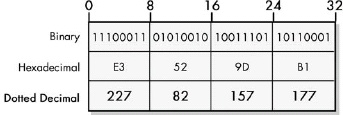
\includegraphics[width=.7\textwidth]{images/ip-address-notation.jpg}
   \caption{IP address binary, hexadecimal, and dotted decimal representations -- The binary, hexadecimal, and decimal representations of an IP address are all equivalent.}
   \label{fig:ip-address-notation}
\end{figure}

Dotted decimal notation provides a convenient way to work with
\protect\hypertarget{ch16s02.htmlux5cux23idx-CHP-16-0658}{}{}IP
addresses when communicating among people. Never forget that to the
computers, the IP address is always a 32-bit
\protect\hypertarget{ch16s02.htmlux5cux23idx-CHP-16-0659}{}{}binary
number; you'll understand the importance of this when you look at how
the IP address is logically divided into components in the next topic,
and when you examine techniques that manipulate IP addresses, such as
subnetting.



\subsection{IP address space}

Since the IP address is 32 bits wide, this provides a theoretical {\emph{address
space}} of $2^{32}$, or 4,294,967,296 addresses.
This seems like quite a lot of addresses, and in some ways, it is.
However, as you will see, due to how IP addresses are structured and allocated, not every one of those addresses can actually be used.

One of the unfortunate legacies of the fact that IP was originally
created on a rather small internetwork is that decisions were made that
wasted much of the address space. For example, all IP addresses starting
with 127 in the first octet are reserved for the loopback function. Just
this one decision makes 1/256th of the total number, or 16,277,216
addresses, no longer available. There are also other ways that the IP
address space was not conserved. This caused difficulty as the Internet
grew in size. (You'll see more about this in \vref{chap:kozierok-ch17}, which covers classful addressing.)


{\textbf{KEY CONCEPT}} Since IP addresses are 32 bits long, the total
address space of IPv4 is $2^{32}$ or 4,294,967,296 addresses.
However, not all of these addresses can be used, for a variety of reasons.

This IP address space dictates the limit on the number of addressable
interfaces in {\emph{each}} IP internetwork. So, if you have a private
network, you can, in theory, have four-billion-plus addresses. However,
in a public network such as the Internet, alldevices must share the
available address space. Techniques such as Classless Inter-Domain
Routing (CIDR), or supernetting, and NAT were designed in part to
utilize the existing Internet IP address space more efficiently. IPv6
expands the IP address size from 32 bits all the way up to 128, which
increases the address space to a ridiculously large number and makes the
entire matter of address space size moot.



\section{IP basic address structure and main components}

As I mentioned in the IP addressing overview, one of the ways that IP
addresses are used is to facilitate the routing of datagrams in an IP
internetwork. This is made possible because of the way that IP addresses
are structured and how that structure is interpreted by network routers.



\subsection{Network ID and host ID}

As you just saw, each IPv4 address is 32 bits long.
When you refer to the IP address, you use a dotted decimal notation, while the computer converts
this into binary. However, even though these sets of 32 bits are
considered a single entity, they have an internal structure containing
two components:
\begin{description}
   \item[Network identifier (network ID)]
      A certain number of bits, starting from the leftmost bit, is used to identify the network where the host or other network interface is located. This is also sometimes called the \emph{network prefix} or even just the \emph{prefix}.
   \item[Host identifier (host ID)]
      The remainder of the bits is used to identify the host on the network.
\end{description}

\subsubsection[Note]{\texorpdfstring{\protect\hypertarget{ch16s03.htmlux5cux23note-62}{}{}Note}{Note}}

{\emph{By convention, IP devices are often called hosts for simplicity,
as I do throughout this book. Even though each host usually has a single
IP address, you should remember that IP addresses are strictly
associated with network layer network interfaces, not physical devices,
and a device may therefore have more than one IP address (especially a
router or multihomed host)}}.

As you can see in \cref{fig:ip-address-division},
this really is a fairly simple concept. The fundamental division of the
bits of an IP address is into a network ID and host ID. In this
illustration, the network ID is 8 bits long, and the host ID is 24 bits
in length. This is similar to the structure used for phone numbers in
North America. The telephone number (401) 555-7777 is a ten-digit number
that's usually referred to as a single phone number. However, it has a
structure. In particular, it has an area code (401) and a local number
(555-7777).

The fact that the network ID is contained in the IP address is what
partially facilitates the routing of IP datagrams when the address is
known. Routers look at the network portion of the IP address to first
determine if the destination IP address is on the same network as the
host IP address. Then routing decisions are made based on information
the routers keep about where various networks are located. Again, this
is conceptually similar to how the area code is used by the equivalent
of routers in the phone network to switch telephone calls. The host
portion of the address is used by devices on the local portion of the
network.

\begin{figure}
   \centering
   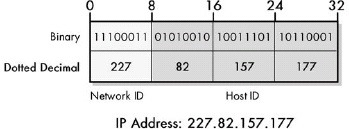
\includegraphics[width=.6\textwidth]{images/ip-address-division.jpg}
   \caption{Basic IP address division: network ID and host ID -- This diagram shows one of the many ways to divide an IP address into a network ID and host ID.}
   \label{fig:ip-address-division}
\end{figure}



\subsection{Location of the Division Between Network ID and Host ID}

One difference between IP addresses and phone numbers is that the
dividing point between the bits used to identify the network and those
that identify the host isn't fixed. It depends on the nature of the
address, the type of addressing being used, and other factors.

Take the previous example of 227.82.157.177 (see
\protect\hyperlink{ch16s02.htmlux5cux23ip_address_binary_hexadecimal_and_dotted}{Figure~16-2}).
It is possible to divide this into a network ID of 227.82 and a host ID
of 157.177. Alternatively, the network ID might be 227 and the host ID
might be 82.157.177 within that network.

To express the network and host IDs as 32-bit addresses, you add zeros
to replace the missing pieces. With a network ID of 227 and a host ID of
82.157.177, the address of the network becomes 227.0.0.0 and the address
of the host 0.82.157.177. (In practice, network addresses of this sort
are routinely seen with the added zeros; network IDs are not seen as
often in 32-bit form this way.)

Lest you think from these examples that the
\protect\hypertarget{ch16s03.htmlux5cux23idx-CHP-16-0663}{}{}division
must always be between whole octets of the address, you should know that
it's also possible to divide it in the middle of an octet. For example,
you could split the IP address 227.82.157.177 so that there were 20 bits
for the network ID and 12 bits for the host ID. The process is the same,
but determining the dotted decimal ID values is more tricky because
here, the 157 is split into two binary numbers. The results are
227.82.144.0 for the network ID and 0.0.0.13.177 for the host ID, as
shown in
\protect\hyperlink{ch16s03.htmlux5cux23mid-octet_ip_address_division_ip_address}{Figure~16-4}.

Since IP addresses are normally expressed as four dotted-decimal
numbers, educational resources often show the division between the
network ID and host ID occurring on an octet boundary. However, it's
essential to remember that the dividing point often appears in the
middle of one of these eight-bit numbers. In
\protect\hyperlink{ch16s03.htmlux5cux23mid-octet_ip_address_division_ip_address}{Figure~16-4},
the network ID is 20 bits long, and the host ID 12 bits long. This
results in the third number of the original IP address, 157, being split
into 144 and 13.

The place where the line is drawn between the network ID and the host ID
must be known in order for devices such as routers to know how to
interpret the address. This information is conveyed either implicitly or
explicitly, depending on the type of IP addressing in use, as I discuss
next.

\protect\hypertarget{ch16s03.htmlux5cux23mid-octet_ip_address_division_ip_address}{}{}

\protect\hypertarget{ch16s03.htmlux5cux23I_mediaobject2_d1e16127}{}{}
%\includegraphics{httpatomoreillycomsourcenostarchimages287797.png.jpg}

Figure~16-4.~Mid-octet IP address division IP addresses need not be
divided between network ID and host ID on octet boundaries. The division
here is into a 20-bit network ID and a 12-bit host ID.


{\textbf{KEY CONCEPT}} The basic structure of an IP address consists of
two components: the network ID and host ID. The dividing point of the
32-bit address is not fixed, but depends on a number of factors and can
occur in a variety of places, including in the middle of a
dotted-decimal octet.

Since the IP address can be split into network ID and host ID
components, it is also possible to use either one or the other by
itself, depending on context. These addresses are assigned special
meanings. For example, if the network ID is used with all ones as the
host ID, this indicates a broadcast to the entire network. Similarly, if
the host ID is used by itself with all zeros for the network ID, this
implies an IP address sent to the host of that ID on the local network,
whatever that might be.
This is explained in much more detail in \vref{chap:kozierok-ch17}.

It is the inclusion of the network ID in the IP address of each host on
the network that causes the IP addresses to be network-specific. If you
move a device from one network to a different one, the network ID must
change to that of the new network. Therefore, the IP address must change
as well. This is an unfortunate drawback that shows up most commonly
when dealing with mobile devices; see
\protect\hyperlink{ch30.html}{Chapter~30}.


\section{IP addressing categories and IP address adjuncts}

We just explored how the 32 bits in an IP address are fundamentally divided into
the network ID and host ID. The network ID is used for routing purposes,
and the host ID uniquely identifies each network interface on the
network. In order for devices to know how to use IP addresses on the
network, they must be able to tell which bits are used for each ID.
However, the dividing line is not predefined. It depends on the type of
addressing used in the network.

Understanding how these IDs are determined leads us into a larger
discussion of the three main categories of IP addressing schemes:
classful, subnetted, and classless. Each of these uses a slightly
different system of indicating where in the IP address the host ID is
found.



\subsection{Conventional (classful) addressing}

The original IP addressing scheme is set up so that the dividing line
occurs only in one of a few locations: on octet boundaries. Three main
classes of addresses -- A, B, and C -- are differentiated based on how
many octets are used for the network ID and how many for the host ID.
For example, class C addresses devote 24 bits to the network ID and 8
bits to the host ID. This type of addressing is now often referred to by
the made-up word {\emph{classful}} to differentiate it from the newer
classless scheme.

This most basic addressing type uses the simplest method to divide the
network and host IDs: The class, and therefore the dividing point, are
encoded into the first few bits of each address. Routers can tell from
these bits which octets belong to which identifier.




\subsection{Subnetted classful addressing}

In the subnet addressing system, the two-tier network and host division
of the IP address is made into a three-tier system by taking some number
of bits from a class A, B, or C host ID and using them for a
{\emph{subnet identifier (subnet ID)}}. The network ID is unchanged. The
subnet ID is used for routing within the different subnetworks that
constitute a complete network, thereby providing extra flexibility for
administrators. For example, consider a class C address that normally
uses the first 24 bits for the network ID and remaining 8 bits for the
host ID. The host ID can be split into, say, 3 bits for a subnet ID and
5 bits for the host ID.

This system is based on the original classful scheme, so the dividing
line between the network ID and full host ID is based on the first few
bits of the address as before. The dividing line between the subnet ID
and the "subhost" ID is indicated by a 32-bit number called a
{\emph{subnet mask}}. In the previous example, the subnet mask would be
27 ones followed by 5 zeros -- the zeros indicate what part of the
address is the host. In dotted decimal notation, this would be
255.255.255.224.




\subsection{Classless addressing}

In the classless system, the classes of the original IP addressing
scheme are tossed out the window. The division between the network ID
and host ID can occur at an arbitrary point, not just on octet
boundaries, as in the classful scheme.

The dividing point is indicated by putting the number of bits used for
the network ID, called the {\emph{prefix length}}, after the address.
(Recall that the network ID bits are also sometimes called the
{\emph{network prefix}}, so the network ID size is the prefix length.)
For example, if 227.82.157.177 is part of a network where the first 27
bits are used for the network ID, that network would be specified as
227.82.157.160/27. The /27 is conceptually the same as the
255.255.255.224 subnet mask, since it has 27 one bits followed by 5
zeros.


{\textbf{KEY CONCEPT}} An essential factor in determining how an IP
address is interpreted is the addressing scheme in which it is used. The
three methods, arranged in increasing order of age, complexity, and
flexibility, are classful addressing, subnetted classful addressing, and
classless addressing.

This introduction to the concepts of classful, subnetted, and classless
addressing was designed to show you how they impact the way the IP
address is interpreted. I have greatly summarized important concepts
here. All three methods are explained in their own chapters in full
detail.




\subsection{Subnet mask and default gateway}

In the original classful scheme, the division between network ID and host ID is
implied.
However, if either subnetting or classless addressing is used, then the {\emph{subnet mask}} (or {\emph{slash number}}, which is equivalent) is required to fully qualify the address.
These numbers are considered adjuncts to the IP address and usually mentioned with the address itself, because without them, it is not possible to know where the network ID ends and the host ID begins.

One other number that is often specified along with the IP address for a
device is the
\protect\hypertarget{ch16s04.htmlux5cux23idx-CHP-16-0666}{}{}{\emph{default
gateway}} identifier. In simplest terms, this is the IP address of the
router that provides default routing functions for a particular device.
When a device on an IP network wants to send a datagram to a device it
can't see on its local IP network, it sends it to the default gateway,
which takes care of routing functions. Without this, each IP device
would also need to have knowledge of routing functions and routes, which
would be inefficient. See \protect\hyperlink{ch23.html}{Chapter~23},
which discusses IP routing concepts, and
\protect\hyperlink{ch37.html}{Chapter~37} through 41, which cover TCP/IP
routing protocols, for more information.


\section{Number of IP addresses and multihoming}
Each network interface on an IP internetwork has a separate IP address.
In a classic network, each regular computer, usually called a
{\emph{host}}, attaches to the network in exactly only one place, so it
will have only one IP address. This is what most of us are familiar with
when using an IP network (and is also why most people use the term
{\emph{host}} when they really mean {\emph{network interface}}).

If a device has more than one interface to the internetwork, it will
have more than one IP address. The most obvious case where this occurs
is with routers, which connect together different networks and thus must
have an IP address for the interface on each one. It is also possible
for hosts to have more than one IP address, however. Such a device is
sometimes said to be {\emph{multihomed}}.

There are two ways that a host can be multihomed:

{\textbf{Two or More Interfaces to the Same Network}} Devices such as
servers or high-powered workstations may be equipped with two physical
interfaces to the same network for performance and reliability reasons.
They will have two IP addresses on the same network with the same
network ID.

{\textbf{Interfaces to Two or More Different Networks}} Devices may have
multiple interfaces to different networks. The
\protect\hypertarget{ch16s05.htmlux5cux23idx-CHP-16-0669}{}{}IP
addresses will typically have different network IDs in them.

\protect\hyperlink{ch16s06.htmlux5cux23multihomed_devices_on_an_ip_internetwork}{Figure~16-5}
shows examples of both types of multihomed device. Of course, these
could be combined, with a host having two connections to one network and
a third to another network. There are also some other special cases,
such as a host with a single network connection having multiple IP
address aliases.

\subsubsection[Note]{\texorpdfstring{\protect\hypertarget{ch16s05.htmlux5cux23note-63}{}{}Note}{Note}}

{\emph{When subnetting is used, the same distinction can be made between
multihoming to the same subnet or a different subnet}}.

Now, let's consider the second case. If a host has interfaces to two or
more different networks, could it pass IP datagrams between them? Yes,
if it had the right
\protect\hypertarget{ch16s05.htmlux5cux23idx-CHP-16-0670}{}{}software
running on it. And wouldn't that make the host a router, of sorts? In
fact, that is exactly the case. A multihomed host with interfaces to two
networks can use software to function as a router. This is sometimes
called
\protect\hypertarget{ch16s05.htmlux5cux23idx-CHP-16-0671}{}{}{\emph{software
routing}}.

Using a host as a router has certain advantages and disadvantages
compared to a hardware router. A server that is multihomed can perform
routing functions and also, well, act as a server. A dedicated hardware
router is designed for the job of routing and usually will be more
efficient than a software program running on a host.


{\textbf{KEY CONCEPT}} A host with more than one IP network interface is
said to be multihomed. A multihomed device can have multiple connections
to the same network, to different networks, or both. A host connected to
two networks can be configured to function as a router.

Multihoming was once considered a fairly esoteric application, but has
become more common in recent years. This is also true of multihoming on
different networks for software routing use. In fact, you may be doing
this in your home without realizing it.

Suppose you have two PCs networked together and a single phone line to
connect to the Internet. One computer dials up to your Internet service
provider (ISP) and runs software such as Microsoft's
\protect\hypertarget{ch16s05.htmlux5cux23idx-CHP-16-0672}{}{}Internet
Connection Sharing
(\protect\hypertarget{ch16s05.htmlux5cux23idx-CHP-16-0673}{}{}ICS) to
let the other computer access the Internet. Millions of people do this
every day -- they have a multihomed system (the one connecting to the
Internet and the other PC) with ICS acting in the role of a software
router (though there are some technical differences between ICS and a
true router, of course).


\section{IP address management and assignment methods and authorities}
What would happen if you told someone that you lived at 34 Elm Street, and when he
turned onto your road, he found four different houses with the number 34
on them? He probably would find your place eventually but wouldn't be
too pleased. Neither would you or your mail carrier! And all of you
folks are much smarter than computers. Like street addresses, IP
addresses must be unique for them to be useful.

\protect\hypertarget{ch16s06.htmlux5cux23multihomed_devices_on_an_ip_internetwork}{}{}

\protect\hypertarget{ch16s06.htmlux5cux23I_mediaobject2_d1e16338}{}{}
%\includegraphics{httpatomoreillycomsourcenostarchimages287799.png.jpg}

Figure~16-5.~Multihomed devices on an IP internetwork This internetwork
consists of two LANs, A (above) and B (below). LAN A has a multihomed
workstation, shown with two IP network interface "circles." The two LANs
are connected together through a multihomed, shared server that has been
configured to route traffic between them. Note that this server also
handles all traffic passing between LAN B and the Internet (since the
Internet connection is in LAN A only).

Since IP datagrams are sent only within the confines of the IP
internetwork, they must be unique within each internetwork. If you are a
company with your own private internetwork, this isn't really a big
problem. Whoever is in charge of maintaining the internetwork keeps a
list of what numbers have been used where and makes sure that no two
\protect\hypertarget{ch16s06.htmlux5cux23idx-CHP-16-0675}{}{}devices are
given the same address. However, what happens in a public network with
many different organizations? Here, it is essential that the IP address
space be managed across the organizations to ensure that they use
different addresses. It's not feasible to have each organization
coordinate its activities with each other one. Therefore, some sort of
centralized {\emph{management authority}} is required.

At the same time that you need someone to ensure that there are no
conflicts in address assignment, you don't want users of the network to
have to go to this central authority every time they need to make a
change to their network. It makes more sense to have the authority
assign numbers in blocks or chunks to organizations based on the number
of devices they want to connect to the network. The organizations can
manage those blocks as they see fit, and the authority's job is made
easier because it deals in blocks instead of billions of individual
addresses and machines.

The Internet, as the big IP internetwork, requires this coordination
task to be performed for millions of organizations worldwide. The job of
managing IP address assignment on the Internet was originally carried
out by a single organization: the {\emph{Internet Assigned Number
Authority (IANA)}}. IANA was responsible for allocating IP addresses,
along with other important centralized coordination functions such as
managing universal parameters used for TCP/IP protocols. In the late
1990s, a new organization called the {\emph{Internet Corporation for
Assigned Names and Numbers (ICANN)}} was created. ICANN now oversees the
IP address assignment task of IANA, as well as managing other tasks such
as Domain Name System (DNS) name registration (see
\protect\hyperlink{ch54.html}{Chapter~54}).

IP addresses were originally allocated directly to organizations. The
original IP addressing scheme was based on classes, and so IANA would
assign addresses in class A, B, and C blocks. Today, addressing is
classless, using CIDR's hierarchical addressing scheme. IANA doesn't
assign addresses directly, but rather delegates them to regional
Internet registries (RIRs). These are APNIC, ARIN, LACNIC, and RIPE NCC.
Each RIR can, in turn, delegate blocks of addresses to lower-level
registries such as national Internet registries (NIRs) and local
Internet registries (LIRs).

Eventually, blocks of addresses are obtained by ISPs for distribution to
end-user organizations. Some of the ISP's customers are end-user
organizations, but others are (smaller) ISPs themselves. They can, in
turn, use or delegate the addresses in their blocks. This can continue
for several stages in a hierarchical fashion. This arrangement helps
ensure that IP addresses are assigned and used in the most efficient
manner possible. See \vref{chap:kozierok-ch20}, which
discusses CIDR, for more information on how this works.

IANA, ICANN, and the RIRs are responsible for more than just IP address
allocation, though I have concentrated on IP addresses here for obvious
reasons. For more general information on IANA, ICANN, APNIC, ARIN,
LACNIC, and RIPE NCC, try a can of alphabet soup -- or \protect\hyperlink{ch03.html}{Chapter~3}, which provides an overview of the Internet registration authorities.





% Kozierok, ch. 17
\chapter{Classful (conventional) addressing}
\label{chap:kozierok-ch17}

The original addressing method for IP addresses divided the IP address
space into five chunks of different sizes called {\emph{classes}}, and
assigned blocks of addresses to organizations from these classes based
on the size and requirements of the organization. In this classful
addressing scheme, each class is reserved for a particular purpose, with
the main address classes differentiated based on how many octets are
used for the network identifier (network ID) and how many are used for
the host identifier (host ID).

In this chapter, I describe classful IP addressing. I begin with an
overview of the concept and general description of the different
classes. I discuss the network and host IDs and address ranges
associated with the different classes. I discuss the capacities of each
of the commonly used classes, meaning how many networks belong to each
and how many hosts each network can contain. I discuss the special
meanings assigned to certain IP address patterns and the special ranges
reserved for private IP addressing, loopback functions, and
multicasting. I conclude with a discussion of the problems with this
type of addressing, which led to it being abandoned in favor of
subnetting, and eventually, classless assignment of the
\protect\hypertarget{ch17.htmlux5cux23idx-CHP-17-0676}{}{}IP address
space.

\subsubsection[Note]{\texorpdfstring{\protect\hypertarget{ch17.htmlux5cux23note-64}{}{}Note}{Note}}

\emph{The classful addressing scheme has been replaced by the classless addressing system described in \vref{chap:kozierok-ch20}.
However, I think it is still important to understand how this original system operates, as it forms the basis for the more sophisticated addressing mechanisms.}



\section{IP classful addressing overview and address classes}

The developers of the Internet Protocol (IP) recognized that organizations come in different sizes and would therefore need varying
numbers of IP addresses on the Internet.
They devised a system to divide the IP address space into {\emph{classes}}, each of which contained a portion of the total addresses and was dedicated to specific uses.
Some classes would be devoted to large networks on the Internet, while others would be reserved for smaller organizations or special purposes.

This original system had no name; it was simply ``the'' IP addressing system.
Today it is called the \emph{classful addressing scheme} to differentiate it from the newer classless scheme.



\subsection{IP address classes}

There are five classes in the classful system, which are assigned the letters~A through~E.
\Cref{tab:ip-address-classes} provides some general information about the classes, their intended uses, and their characteristics.

\begin{table}
   \begin{tabular}{lrrrl}
   \toprule
   class      & fraction & NID & HID & intended use\\
   \midrule
   \textbf{A} & 1/2      & 8   & 24  & Unicast for very large organizations\\
   \textbf{B} & 1/4      & 16  & 16  & Unicast for medium to large organizations\\
   \textbf{C} & 1/8      & 24  & 8   & Unicast for smaller organizations\\
   \textbf{D} & 1/16     & n/a & n/a & IP multicasting\\
   \textbf{E} & 1/16     & n/a & n/a & Reserved for experimental use\\
   \bottomrule
   \end{tabular}
   \caption{IP Address Classes and class Characteristics and Uses}
   \label{tab:ip-address-classes}
\end{table}

Looking at this table (and \cref{fig:ipv4-classes}), you can see that Classes A, B, and C take up most of the total address space (seven-eighths of it).
These are the classes used for {\emph{unicast}} IP addressing and messages sent to a single network interface.
(The blocks also include associated broadcast addresses for these networks.)
This is what I usually consider normal IP addressing.


\begin{figure}
   \centering
   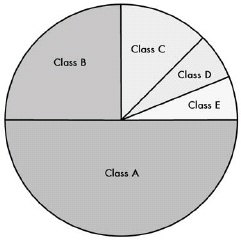
\includegraphics[width=.5\textwidth]{images/ipv4-classes.jpg}
   \caption{Division of IPv4 address space into classes}
   \label{fig:ipv4-classes}
\end{figure}

You can think of Classes A, B, and C as the papa bear, mama bear, and baby bear of traditional IP addressing.
They allow the Internet to provide addressing for a small number of very
large networks, a moderate number of medium-sized organizations, and a
large number of smaller companies. This approximately reflects the
distribution of organization sizes in the real world, though the large
gulf in the maximum number of hosts allowed for each address class leads
to inflexibility, as I will discuss later in the chapter.

As you can see, the classes differ in where they draw the line between
the network ID and the host ID portions of the addresses they contain.
However, in each case, the division is made on octet boundaries. In
classful addressing, the division does not occur within an octet.

Classes D and E are special -- to the point where many people don't even realize they exist.
class D is used for IP multicasting, while class E is reserved for experimental use (by the designers of the Internet).
I discuss IP multicast addressing later in this chapter.


{\textbf{KEY CONCEPT}} The classful IP addressing scheme divides the IP
address space into five classes, A through E, of differing sizes.
Classes A, B, and C are the most important ones, designated for
conventional unicast addresses and taking up seven-eighths of the
address space. class D is reserved for IP multicasting, and class E is
reserved for experimental use.



\subsection{Rationale for classful addressing}

While the drawbacks of the classful system are often discussed today (as
you'll see later in this chapter), it's important to keep in context
what the size of the Internet was when this system was developed. The
Internet was tiny then, and the 32-bit address space seemed enormous by
comparison to even the number of machinesits creators envisioned years
into the future. It's only fair to also remember the following
advantages of the classful system developed over 25 years ago:

\begin{description}
   \item[Simplicity and clarity]
      There are only a few classes to choose from, and it's very simple to understand how the addresses are split up.
      The distinction between classes is clear and obvious.
      The divisions between network ID and host ID in Classes A, B, and C are on octet boundaries, making it easy to tell what the network ID is of any address.

   \item[Reasonable flexibility]
      Three levels of granularity match the sizes of large, medium-sized, and small organizations reasonably well.
      The original system provided enough capacity to handle the anticipated growth rate of the Internet at the time.

   \item[Routing ease]
      As you will see shortly, the class of the address is encoded right into the address to make it easy for routers to know what part of any address is the network ID and what part is the host ID.
      There was no need for adjunct information such as a subnet mask.

   \item[Reserved addresses]
      Certain addresses are reserved for special purposes.
      This includes not just Classes D and E, but also special reserved address ranges for private addressing.
   \end{description}

Of course, it turned out that some of the decisions in the original IP addressing scheme were regrettable -- but that's the benefit of hindsight.
I'm sure we would all like to have back the 268-odd million addresses that were set aside for class E.
While it may seem wasteful now to have reserved a full one-sixteenth of the address space for experimental use, remember that the current size of the Internet was never anticipated even 10 years ago, never mind 25.
Furthermore, it's good practice to reserve some portion of any scarce resource for future use.




\section{IP classful addressing network and host identification and address ranges}

The classful IP addressing scheme divides the total IP address space
into five classes, A through E. One of the benefits of the relatively
simple classful scheme is that information about the classes is encoded
directly into the IP address. This means you can determine in advance
which address ranges belong to each class. It also means the opposite is
possible: You can identify which class is associated with any address by
examining just a few bits of the address. This latter benefit was one of
the main motivators for the initial creation of the classful
system.\protect\hypertarget{ch17s02.htmlux5cux23idx-CHP-17-0685}{}{}


\subsection{Classful addressing class determination algorithm}

When TCP/IP was first created, computer technology was still in its
infancy. Routers needed to be able to quickly make decisions about how
to move IP datagrams around. The IP address space was split into classes
in such a way that, by looking at only the first few bits of any IP
address, the router could easily tell how to choose between the network
and host ID, and thus what to do with the datagram.

The number of bits the router needs to look at may be as few as one or
as many as four, depending on what it finds when it starts looking. The
algorithm used to determine the class corresponds to the system used to
divide the address space, as illustrated in \cref{fig:class-determination}.


\begin{figure}
   \centering
   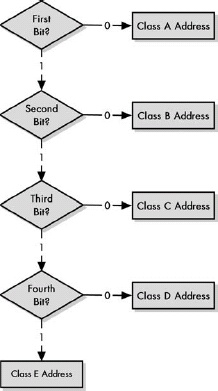
\includegraphics[width=.5\textwidth]{images/class-determination.jpg}
   \caption[Class determination algorithm for classful IP addresses]{Class determination algorithm for classful IP addresses -- The simplicity of the classful IP addressing can be seen in the very uncomplicated algorithm used to determine the class of an address.}
   \label{fig:class-determination}
\end{figure}


Here are the four very basic steps in the algorithm:

\begin{enumerate}
   \item
      If the first bit is a 0, it's a class A address, and you're done.
      (Half the address space has a 0 for the first bit, so this is why class A takes up half the address space.)
      If it's a 1, continue to step 2.
   \item
      If the second bit is a 0, it's a class B address, and you're done.
      (Half of the remaining non-class A addresses, or one quarter of the total.)
      If it's a 1, continue to step 3.
   \item
      If the third bit is a 0, it's a class C address, and you're done.
      (Half again of what's left, or one-eighth of the total.) 
      If it's a 1, continue to step 4.
   \item
      If the fourth bit is a 0, it's a class D address.
      (Half the remainder, or one-sixteenth of the address space.) 
      If it's a 1, it's a class E address.
      (The other half, one-sixteenth.)
\end{enumerate}

And that's pretty much it.



\subsection{Determining address class from the first octet bit pattern}

As humans, of course, we generally work with addresses in dotted decimal
notation and not in binary, but it's pretty easy to see the ranges that
correspond to the classes. For example, consider class B. The first two
bits of the first octet are 10. The remaining bits can be any
combination of ones and zeros. This is normally represented as 10xx xxxx
(shown as two groups of four for readability). Thus, the binary for the
first octet can range from {\textbf{10}}00 0000 to {\textbf{10}}11 1111
(128 to 191 in decimal). So in the classful scheme, any IP address whose
first octet is between 128 and 191 inclusive is a class B address.

\protect\hyperlink{ch17s02.htmlux5cux23ip_address_class_bit_patterns_first-octe}{Table~17-2}
shows the bit patterns for each of the five classes and the way that the first octet
ranges can be calculated. The first column shows the format of the first
octet of the IP address; the {\emph{x}}s can be either a zero or a one.
Next are the lowest and highest value columns for each class in binary
(the fixed few bits are in bold print so you can see that they do not
change while the others do), followed by the corresponding range for the
first octet, in decimal.

\protect\hypertarget{ch17s02.htmlux5cux23ip_address_class_bit_patterns_first-octe}{}{}

Table~17-2.~IP Address class Bit Patterns, First-Octet Ranges, and
Address Ranges

\begin{longtable}[]{@{}lllllll@{}}
\toprule
Class & First octet & Lowest value & Highest value & Range & Octets in Network ID/Host ID & Theoretical IP Address Range\tabularnewline
\midrule
\endhead
class A & \textbf{0}xxx xxxx & {\textbf{0}}000 0001 & {\textbf{0}}111 1110 & 1--127 & 1 / 3 & 1.0.0.0 to 127.255.255.255\\
class B & \textbf{10}xx xxxx & {\textbf{10}}00 0000 & {\textbf{10}}11 1111 & 128--191 & 2 / 2 & 128.0.0.0 to 191.255.255.255\\
class C & \textbf{110}x xxxx & {\textbf{110}}0 0000 & {\textbf{110}}1 1111 & 192--223 & 3 / 1 & 192.0.0.0 to 223.255.255.255\\
class D & \textbf{1110} xxxx & {\textbf{1110}} 0000 & {\textbf{1110}} 1111 & 224--239 & --- & 224.0.0.0 to 239.255.255.255\\
class E & \textbf{1111} xxxx & {\textbf{1111}} 0000 & {\textbf{1111}} 1111 & 240--255 & --- & 240.0.0.0 to 255.255.255.255\\
\bottomrule
\end{longtable}

This table also shows the {\emph{theoretical}} lowest and highest IP
address ranges for each of the classes. This means that they are the
result of taking the full span of binary numbers possible in each class.
In reality, some of the values are not available for normal use. For
example, even though the range 192.0.0.0 to 192.0.0.255 is technically
in class C, it is reserved and not actually used by hosts on the
Internet.

Also, certain IP addresses cannot be used because they have special
meaning. For example, 255.255.255.255 is a reserved broadcast address.

Recall that Classes A, B, and C differ in where the dividing line is
between the network ID and the host ID: 1 for network and 3 for host for
class A, 2 for each for class B, and 3 for network and 1 for host for
class C. Based on this division, in
\protect\hyperlink{ch17s02.htmlux5cux23ip_address_class_bit_patterns_first-octe}{Table~17-2},
I have highlighted the network ID portion of the IP address ranges for
each of Classes A, B, and C. The plain text corresponds to the range of
host IDs for each allowable network ID.
\protect\hyperlink{ch17s02.htmlux5cux23ip_address_class_bit_assignments_and_net}{Figure~17-3}
shows graphically how bits are used in each of the five classes.

\protect\hypertarget{ch17s02.htmlux5cux23ip_address_class_bit_assignments_and_net}{}{}

\protect\hypertarget{ch17s02.htmlux5cux23I_mediaobject3_d1e16900}{}{}
%\includegraphics{httpatomoreillycomsourcenostarchimages287805.png.jpg}

Figure~17-3.~IP address class bit assignments and network/host ID sizes
This illustration shows how the 32 bits of IP address are assigned for
each of the five IP address classes. Classes A, B, and C are the normal
classes used for regular unicast addresses; each has a different
dividing point between the network ID and host ID. Classes D and E are
special and are not divided in this manner.


{\textbf{KEY CONCEPT}} In the classful IP addressing scheme, the class
of an IP address is identified by looking at the first one, two, three,
or four bits of the address. This can be done both by humans working
with these addresses and routers making routing decisions. The use of
these bit patterns means that IP addresses in different classes fall
into particular address ranges that allow an address's class to be
determined by looking at the first byte of its dotted decimal
address.\protect\hypertarget{ch17s02.htmlux5cux23idx-CHP-17-0693}{}{}

For example, consider class C. The lowest IP address is
{\textbf{192.0.0}}.0, and the highest is {\textbf{223.255.255}}.255. The
first three octets are the network ID and can range from
{\textbf{192.0.0}} to {\textbf{223.255.255}}. For each network ID in
that range, the host ID can range from 0 to 255.

\subsubsection[Note]{\texorpdfstring{\protect\hypertarget{ch17s02.htmlux5cux23note-65}{}{}Note}{Note}}

{\emph{It is common to see resources refer to the network ID of a
classful address as including only the significant bits; that is, only
the ones that are not common to all networks of that class. For example,
you may see a class B network ID shown in a diagram as having 14 bits,
with the 10 that starts all such networks shown separately, as if it
were not part of the network ID. Remember that the network ID does
include those bits as well; it is 8 full bits for class A, 16 for Class
B, and 24 for class C. In the case of class D addresses, all 32 bits are
part of the address, but only the lower 28 bits are part of the
multicast group address; see the topic on multicast addressing later in
this chapter for more}}.


\section{IP address class A, B, and C network and host capacities}

So far, I have introduced the concepts of IP address classes and showed
how the classes relate to ranges of IP addresses. Of the five classes, D
and E are dedicated to special purposes, so I will leave those alone for
now. Classes A, B, and C are the ones actually assigned for normal
(unicast) addressing purposes on IP internetworks, and therefore they
are the primary focus of our continued attention.

As you've seen, the classes differ in the number of bits (and octets)
used for the network ID compared to the host ID. The number of different
networks possible in each class is a function of the number of bits
assigned to the network ID, and likewise, the number of hosts possible
in each network depends on the number of bits provided for the host ID.
You must also take into account the fact that one, two, or three of the
bits in the IP address are used to indicate the class itself, so it is
effectively excluded from use in determining the number of networks
(though again, it is still part of the network ID).

Based on this information, you can calculate the number of networks in
each class, and for each class, the number of host IDs per network.
\protect\hyperlink{ch17s03.htmlux5cux23ip_address_class_network_and_host_capaci}{Table~17-3}
shows the calculations.

\protect\hypertarget{ch17s03.htmlux5cux23ip_address_class_network_and_host_capaci}{}{}

Table~17-3.~IP Address Class Network and Host Capacities

\begin{longtable}[]{@{}lllllll@{}}
\toprule
IP Address Class & Total \# of Bits for Network ID/Host ID & First Octet
of IP Address & \# of Network ID Bits Used To Identify Class & Usable \#
of Network ID Bits & Number of Possible Network IDs & \# of Host IDs Per
Network ID\tabularnewline
\midrule
\endhead
{\textbf{class A}} & 8/24 & 0xxx xxxx & 1 & 8-1 = 7 &
2\textsuperscript{7}-2 = 126 & 2\textsuperscript{24}-2 =
16,277,214\tabularnewline
{\textbf{class B}} & 16/16 & 10xx xxxx & 2 & 16-2 = 14 &
2\textsuperscript{14} = 16,384 & 2\textsuperscript{16}-2 =
65,534\tabularnewline
{\textbf{class C}} & 24/8 & 110x xxxx & 3 & 24-3 = 21 &
2\textsuperscript{21} = 2,097,152 & 2\textsuperscript{8}-2 =
254\tabularnewline
\bottomrule
\end{longtable}

Let's walk through one line of this table so you can see how it works
using class B as an example. The basic division is into 16 bits for
network ID and 16 bits for host ID. However, the first 2 bits of all
class B addresses must be 10, so that leaves only 14 bits to uniquely
identify the network ID. This gives us a total of 2\textsuperscript{14}
or 16,384 class B network IDs. For each of these, you have
2\textsuperscript{16} host IDs, less two, for a total of
65,534.\protect\hypertarget{ch17s03.htmlux5cux23idx-CHP-17-0694}{}{}

Why less two? For each network ID, two host IDs cannot be used: the host
ID with all zeros and the ID with all ones. These are addresses with
special meanings, as described in the next section. Also notice that two
is subtracted from the number of network IDs for class A. This is
because two of the class A network IDs (0 and 127) are reserved.

Several other address ranges are set aside in all three of the classes
shown here. They are listed in the "IP Reserved, Private, and Loopback
Addresses" section later in this chapter.


{\textbf{KEY CONCEPT}} In the classful IP addressing scheme, a class A
network contains addresses for about 16 million network interfaces; a
class B network contains about 65,000; and a class C network contains
254.

As you can see, there is quite a disparity in the number of hosts
available for each network in each of these classes. What happens if an
organization needs 1,000
\protect\hypertarget{ch17s03.htmlux5cux23idx-CHP-17-0695}{}{}IP
addresses? It must use either four class Cs or one class B (and in so
doing, waste over 90 percent of the possible addresses in the class B
network). Bear in mind that there are only about 16,000 class B network
IDs available worldwide, and you begin to understand one of the big
problems with classful addressing.


\section{IP addresses with special meanings}

Some IP addresses do not refer directly to specific hardware devices; instead, they are used to refer indirectly to one or more devices.
To draw an analogy with language, most IP addresses refer to proper nouns, like ``John'' or ``the red table in the corner.''
However, some are used more the way you use pronouns such as ``this one'' or ``that group over there.''
I call these IP addresses with \emph{special meanings}.

These special addresses are constructed by replacing the normal network ID or host ID (or both) in an IP address with one of two special patterns:

\begin{description}
   \item[All zeros]
      When the network ID or host ID bits are replaced by a set of all zeros, the special meaning is the equivalent of the pronoun \emph{this}, referring to whatever was replaced.
      It can also be interpreted as \emph{the default} or the \emph{current}.
      For example, if you replace the network ID with all zeros but leave the host ID alone, the resulting address means ``the device with the host ID given, on \emph{this network},'' or ``the device with the host ID specified, on \emph{the default network} or \emph{the current network}.''
   \item[All ones]
      When the network ID or host ID bits are replaced by a set of all ones, this has the special meaning of \emph{all}, meaning that the IP address refers to all hosts on the network.
      This is generally used as a broadcast address for sending a message to everyone.
\end{description}

{\textbf{KEY CONCEPT}} When the network ID or host ID of an IP address
is replaced by a pattern of all ones or all zeros, the result is an
address with a special meaning. Examples of such addresses include ``all hosts'' broadcast addresses and addresses that refer to a specific host or a whole network.

There are many special addresses. A small number apply to the entire
TCP/IP network, while others exist for each network or host ID. Since
two special patterns can be applied to the network ID, host ID, or both,
there are six potential combinations, each of which has its own meaning.
Of these, five are used.

\protect\hyperlink{ch17s04.htmlux5cux23ip_address_patterns_with_special_meaning}{Table~17-4}
describes each of these special meanings and includes examples from
class A, B, and C. Note how an IP address in each of the common classes
can be modified to have special meaning forms. (The first row shows the
examples in their normal form, for reference.)

\protect\hypertarget{ch17s04.htmlux5cux23ip_address_patterns_with_special_meaning}{}{}

Table~17-4.~IP Address Patterns with Special Meanings

Network ID

Host ID

class A Example

class B Example

class C Example

Special Meaning and Description

{\textbf{Network ID}}

{\textbf{Host ID}}

77.91.215.5

154.3.99.6

227.82.157.160

{\textbf{Normal Meaning}}: Refers to a specific device.

{\textbf{Network ID}}

{\textbf{All Zeros}}

77.0.0.0

154.3.0.0

227.82.157.0

{\textbf{The Specified Network}}: This notation,
\protect\hypertarget{ch17s04.htmlux5cux23idx-CHP-17-0696}{}{}with a 0 at
the end of the address, refers to an entire network.

{\textbf{All Zeros}}

{\textbf{Host ID}}

0.91.215.5

0.0.99.6

0.0.0.160

{\textbf{Specified Host on This Network}}: This addresses a host on the
current or default network when the network ID is not known or when it
doesn't need to be explicitly stated.

{\textbf{All Zeros}}

{\textbf{All Zeros}}

0.0.0.0

{\textbf{Me}}: Used by a device to refer to itself when it doesn't know
its own IP address. (Alternatively, "this host," or "the current/default
host.") The most common use is when a device attempts to determine its
address using a host-configuration protocol like DHCP. May also be used
to indicate that any address of a multihomed host may be used.

{\textbf{Network ID}}

{\textbf{All Ones}}

77.255.255.255

154.3.255.255

227.82.157.255

{\textbf{All Hosts on the Specified Network}}: Used for broadcasting to
all hosts on the local network.

{\textbf{All Ones}}

{\textbf{All Ones}}

255.255.255.255

{\textbf{All Hosts on the Network}}: Specifies a global broadcast to all
hosts on the directly connected network. Note that there is no address
that would imply sending to all hosts everywhere on the global Internet,
since this would be very inefficient and costly.

\subsubsection[Note]{\texorpdfstring{\protect\hypertarget{ch17s04.htmlux5cux23note-66}{}{}Note}{Note}}

{\emph{The missing combination from
\protect\hyperlink{ch17s04.htmlux5cux23ip_address_patterns_with_special_meaning}{Table~17-4}
is that of the network ID being all ones and the host ID normal.
Semantically, this would refer to "all hosts of a specific ID on all
networks," which doesn't really mean anything useful in practice, so
it's not used. Note also that, in theory, a special address where the
network ID is all zeros and the host ID is all ones would have the same
meaning as the all-ones limited broadcast address. The latter is used
instead, however, because it is more general, not requiring knowledge of
where the division is between the network ID and the host ID}}.

Since the all-zeros and all-ones patterns are reserved for these special
meanings, they cannot be used for regular
\protect\hypertarget{ch17s04.htmlux5cux23idx-CHP-17-0697}{}{}IP
addresses. This is why, when you looked at the number of hosts per
network in each of the classes, you had to subtract two from the
theoretical maximum: one for the all-zeros case and one for the all-ones
case.\protect\hypertarget{ch17s04.htmlux5cux23idx-CHP-17-0698}{}{}

Similarly, the network ID cannot be all zeros either. However, this
doesn't require specific exclusion because the entire block of addresses
with 0 in the first octet (0.x.x.x) is one of the reserved sets of
\protect\hypertarget{ch17s04.htmlux5cux23idx-CHP-17-0699}{}{}IP
addresses. These reserved addresses, described in the next section,
further restrict the use of certain addresses in the IP address space
for regular uses.



\section{IP reserved, private, and loopback addresses}

In addition to the unusable numbers with special meanings just
discussed, several other sets of IP addresses have special uses, and are
therefore not available for normal address assignment. These generally
fall into three categories: reserved, private, and loopback addresses.

\subsection{Reserved addresses}

Several blocks of addresses were designated as reserved with no specific
indication given as to what they were reserved for. Perhaps they were
set aside for future experimentation or for internal use in managing the
Internet. (In general, it's a good idea to set aside some portion of any
\protect\hypertarget{ch17s05.htmlux5cux23idx-CHP-17-0700}{}{}limited
resource for unanticipated needs.)

A couple of these blocks appear in each of the three main classes (A, B,
and C), at the beginning and end of each class. (All of class D and E
are also reserved, since they aren't used for regular addressing.)



\subsection{Private, unregistered, nonroutable addresses}

You'll recall that in the IP address overview in \vref{chap:kozierok-ch16}, I contrasted private and
public IP addresses. Every IP address on an IP network must be unique.
In the case of a public IP network, addresses are allocated by a central
authority to ensure that there is no overlap. In contrast, on a private
network, you can use whatever addresses you want.

Then why not just pick any random block of class A, B, or C addresses
for your private network and use that? You could, and some people did.
For example, if you weren't connected to the Internet you could use,
say, the class A network 18.x.x.x that is reserved on the Internet to
the
\protect\hypertarget{ch17s05.htmlux5cux23idx-CHP-17-0701}{}{}Massachusetts
Institute of Technology (MIT). Since you aren't connected to MIT, you
would think that wouldn't matter.

However, as the Internet grew, those disconnected private networks
needed to connect to the public Internet after all, and then they had a
conflict. If they used the 18.x.x.x addresses, they would have to
renumber all their devices to avoid getting a big bunch of computer
geeks really angry. (There were, in fact, cases where companies that had
used IP address space belonging to other companies accidentally
connected those machines to the Internet, causing a small amount of
ruckus in the process.)

RFC 1918 (superseding RFC 1597) provided the solution. It defines a set
of unroutable, special address blocks just for private addresses. These
addresses simply don't exist on the public Internet. For this reason,
they are not registered like other public addresses; they are sometimes
called {\emph{unregistered}}. Anyone can use them, but they cannot
connect to the Internet because routers are not programmed to forward
traffic with these address ranges outside of local organizations. RFC
1918 was published to encourage the use of these private blocks in order
to cut down on the number of devices on the public Internet that didn't
really need to be publicly accessible. This was in response to the need
to conserve the public address space.

\subsubsection[Note]{\texorpdfstring{\protect\hypertarget{ch17s05.htmlux5cux23note-67}{}{}Note}{Note}}

{\emph{In order to connect a network using private addressing to the
public Internet, it is necessary to employ additional hardware and
software. A gateway machine can be used as an interface between the
public and private networks. Technologies such as Network Address
Translation (NAT; see \protect\hyperlink{ch28.html}{Chapter~28}) are
often used in conjunction with private IP addresses to allow these hosts
to communicate on the public IP
network}}.\protect\hypertarget{ch17s05.htmlux5cux23idx-CHP-17-0702}{}{}


{\textbf{KEY CONCEPT}} Private address blocks were created to allow
private IP Internets to be created using addresses that were guaranteed
not to conflict with public IP addresses. They are commonly used in
internetworks that aren't connected to the global Internet; devices
using them can also access the global Internet by using NAT.



\subsection{Loopback addresses}

Normally, when a TCP/IP application wants to send information, that
information travels down the protocol layers to IP, where it is
encapsulated in an IP datagram. That datagram then passes down to the
data link layer of the device's physical network for transmission to the
next hop, on the way to the IP
destination.\protect\hypertarget{ch17s05.htmlux5cux23idx-CHP-17-0703}{}{}

However, one special range of addresses, 127.0.0.0 to 127.255.255.255,
is set aside for {\emph{loopback}} functionality. IP datagrams sent by a
host to a 127.x.x.x loopback address are not passed down to the data
link layer for transmission; instead, they loop back to the source
device at the IP level. In essence, this short-circuits the normal
protocol stack; data is sent by a device's layer~3 IP implementation and
then immediately received by it.

This loopback range is used for testing the TCP/IP protocol
implementation on a host. Since the lower layers are short-circuited,
sending to a loopback address allows you to isolate and test the higher
layers (IP and above) without interference from the lower layers.
\protect\hypertarget{ch17s05.htmlux5cux23idx-CHP-17-0704}{}{}127.0.0.1
is the address most commonly used for testing purposes.


{\textbf{KEY CONCEPT}} Portions of the IP address space are set aside
for reserved, private, and loopback addresses.




\subsection{Reserved, private, and loopback addressing blocks}

\protect\hyperlink{ch17s05.htmlux5cux23reserved_private_and_loopback_ip_address}{Table~17-5}
shows all of the special blocks set aside from the normal
\protect\hypertarget{ch17s05.htmlux5cux23idx-CHP-17-0705}{}{}IP address
space in numerical order, with a brief explanation of how each is used.
It lists both the classful and the classless notation representing each of these blocks because the Internet now uses classless addressing, and because some of the private blocks don't correspond to single class A, B, or C networks.

Note especially the private address block from 192.168.0.0 to 192.168.255.255.
This is the size of a class B network, but it isn't class B in the classful scheme, because the first octet of 192 puts it in the class C part of the address space.
It is actually 256 contiguous class C networks.

You may also notice the special class B (/16) block 169.254.x.x.
This is reserved for {\emph{Automatic Private IP Addressing (APIPA)}}, discussed in
\protect\hyperlink{ch64.html}{Chapter~64}.
Systems that are configured to use this feature will automatically assign systems addresses from this block to enable them to communicate even if no server can be found for proper IP address assignment using the Dynamic Host Control Protocol (DHCP).

\protect\hypertarget{ch17s05.htmlux5cux23reserved_private_and_loopback_ip_address}{}{}

Table~17-5.~Reserved, Private, and Loopback IP Addresses

\begin{longtable}[]{@{}lllll@{}}
\toprule
Range Start Address & Range End Address & Classful Address Equivalent &
Classless Address Equivalent & Description\tabularnewline
\midrule
\endhead
{\textbf{0.0.0.0}} & {\textbf{0.255.255.255}} & class A network 0.x.x.x
& 0/8 & Reserved\tabularnewline
{\textbf{10.0.0.0}} & {\textbf{10.255.255.255}} & class A network
10.x.x.x & 10/8 & class A private address block\tabularnewline
{\textbf{127.0.0.0}} & {\textbf{127.255.255.255}} & class A network
127.x.x.x & 127/8 & Loopback address block\tabularnewline
{\textbf{128.0.0.0}} & {\textbf{128.0.255.255}} & class B network
128.0.x.x & 128.0/16 & Reserved\tabularnewline
{\textbf{169.254.0.0}} & {\textbf{169.254.255.255}} & class B network
169.254.x.x & 169.254/16 & class B private address block reserved for
automatic private address allocation (see
\protect\hyperlink{ch64.html}{Chapter~64} for details)\tabularnewline
{\textbf{172.16.0.0}} & {\textbf{172.31.255.255}} & 16 contiguous Class
B networks from 172.16.x.x through 172.31.x.x & 172.16/12 & class B
private address blocks\tabularnewline
{\textbf{191.255.0.0}} & {\textbf{191.255.255.255}} & class B network
191.255.x.x & 191.255/16 & Reserved\tabularnewline
{\textbf{192.0.0.0}} & {\textbf{192.0.0.255}} & class C network
192.0.0.x & 192.0.0/24 & Reserved\tabularnewline
{\textbf{192.168.0.0}} & {\textbf{192.168.255.255}} & 256 contiguous
class C networks from 192.168.0.x through 192.168.255.x & 192.168/16 &
class C private address blocks\tabularnewline
{\textbf{223.255.255.0}} & {\textbf{223.255.255.255}} & class C network
223.255.255.x & 223.255.255/24 & Reserved\tabularnewline
\bottomrule
\end{longtable}


\section{IP multicast addressing}

The vast majority of traffic on IP internetworks is {\emph{unicast}},
which is one source device sending to one destination device. IP also
supports { \emph{multicasting}}, which is a source device sending to a
group of devices. Multicasting is not used a great deal on the
present-day Internet, mainly due to a lack of widespread hardware
support, though it is useful in certain circumstances, especially as a
more efficient alternative to
broadcasting.\protect\hypertarget{ch17s06.htmlux5cux23idx-CHP-17-0707}{}{}

The classful IP addressing scheme sets aside one-sixteenth of the
address space for
\protect\hypertarget{ch17s06.htmlux5cux23idx-CHP-17-0708}{}{}multicast
addresses as class D. Multicast addresses are identified by the pattern
1110 in the first four bits, which corresponds to a first octet of 224
to 239. Thus, the full range of multicast addresses is from 224.0.0.0 to
239.255.255.255.

Since multicast addresses represent a group of IP devices (sometimes
called a {\emph{host group}}), they can be used only as the destination
of a datagram, never the source.



\subsection{Multicast address types and ranges}

The other 28 bits in the IP address define the {\emph{multicast group
address}}. The size of the class D multicast address space is therefore
2\textsuperscript{28}, or 268,435,456 multicast
\protect\hypertarget{ch17s06.htmlux5cux23idx-CHP-17-0709}{}{}groups. No
substructure defines the use of these 28 bits, and there is no specific
concept of a network ID and host ID as in class A, B, and C. However,
certain portions of the address space are set aside for specific uses.
\protect\hyperlink{ch17s06.htmlux5cux23ip_multicast_address_ranges_and_uses}{Table~17-6}
and
\protect\hyperlink{ch17s06.htmlux5cux23ip_multicast_address_ranges_and_uses_all}{Figure~17-4}
show the general allocation of the class D address
space.\protect\hypertarget{ch17s06.htmlux5cux23idx-CHP-17-0710}{}{}\protect\hypertarget{ch17s06.htmlux5cux23idx-CHP-17-0711}{}{}

\protect\hypertarget{ch17s06.htmlux5cux23ip_multicast_address_ranges_and_uses}{}{}

Table~17-6.~IP Multicast Address Ranges and Uses

\begin{longtable}[]{@{}lll@{}}
\toprule
Range Start Address & Range End Address & Description\tabularnewline
\midrule
\endhead
{\textbf{224.0.0.0}} & {\textbf{224.0.0.255}} & Reserved for special
well-known multicast addresses\tabularnewline
{\textbf{224.0.1.0}} & {\textbf{238.255.255.255}} & Globally scoped
(Internetwide) multicast addresses.\tabularnewline
{\textbf{239.0.0.0}} & {\textbf{239.255.255.255}} & Administratively
scoped (local) multicast addresses\tabularnewline
\bottomrule
\end{longtable}

\subsubsection[Note]{\texorpdfstring{\protect\hypertarget{ch17s06.htmlux5cux23note-68}{}{}Note}{Note}}

{\emph{As with the other IP address classes, the entire 32 bits of the
address is always used. It is only the least significant 28 bits that
are interesting, because the upper four bits never change}}.

\protect\hypertarget{ch17s06.htmlux5cux23ip_multicast_address_ranges_and_uses_all}{}{}

\protect\hypertarget{ch17s06.htmlux5cux23I_mediaobject3_d1e17790}{}{}
%\includegraphics{httpatomoreillycomsourcenostarchimages287807.png.jpg}

Figure~17-4.~IP Multicast address ranges and uses All multicast
addresses begin with 1110. The well-known group has zeros for the first
20 bits of the multicast group address, with 8 bits available to define
255 special multicast addresses. Multicast addresses starting with 1110
1111 are locally scoped; all other addresses are globally scoped (this
includes addresses starting with 1110 0000 other than the 255 well-known
addresses).


{\textbf{RELATED INFORMATION}} {\emph{The concept of multicast address
scope was more completely defined in IPv6, and I discuss it in more
detail in the in the discussion of IPv6 multicast addresses in
\protect\hyperlink{ch25.html}{Chapter~25}}}.

The bulk of the address space is in the middle multicast range. These
are normal multicast addresses, like the class A, B, and C unicast
addresses, and they can be assigned to various groups.

The last address range is for {\emph{administratively scoped}} multicast
groups. This is a fancy term for multicast groups used within a private
organization. This block, representing one-sixteenth of the total
multicast address space, is comparable to the private addresses you saw
earlier in this chapter. It is further subdivided into site-local
multicast addresses, organization-local addresses, and so
forth.

\subsection{Well-known multicast addresses}

The first block of 256 addresses is used to define special, well-known multicast address blocks \cref{tab:link-local-multicast} has a selective listing).
These do not represent arbitrary groups of devices and cannot be assigned in that manner.
Instead, they have a
special meaning that allows a source to send a message to a predefined
group.


\begin{table}
   \centering
   \begin{tabular}{rl}
   \emph{multicast address} & description\\[.75ex]
   \textit{224.0.0.0}       & Reserved; not used\\
   \textit{224.0.0.1}       & All devices on the subnet\\
   \textit{224.0.0.2}       & All routers on the subnet\\
   \textit{224.0.0.3}       & Reserved\\
   \textit{224.0.0.4}       & All routers using DVMRP\\
   \textit{224.0.0.5}       & All routers using OSPF\\
   \textit{224.0.0.6}       & Designated routers using OSPF\\
   \textit{224.0.0.9}       & Designated routers using RIP-2\\
   \textit{224.0.0.11}      & Mobile agents (for Mobile IP)\\
   \textit{224.0.0.12}      & DHCP server/relay agent\\
   \end{tabular}
   \caption{IP multicast addresses for the local subnet}
   \label{tab:link-local-multicast}
\end{table}

Delivery of IP multicast traffic is more complex than unicast traffic due to the existence of multiple recipients.
Instead of the normal resolution method through the Address Resolution Protocol (ARP) used for unicast datagrams, the IP multicast group and a hardware multicast group are mapped.




\section{Problems with classful IP addressing}

The classful addressing system was the first major attempt to define a
method for universal addressing of a large IP internetwork. There was a
reasonable rationale for the system, as I mentioned in the overview of
the classful scheme, and given that it was developed decades ago for a
network that was limited in size, it did the job remarkably well for a
long time.

No one ever expected the Internet to mushroom to anything close to its
current size. As the Internet grew, the classful IP addressing mechanism
showed some problems.

The three main problems with classful addressing are as follows:
\begin{description}
   \item[Lack of internal address flexibility]
      Big organizations are assigned large, monolithic blocks of addresses that aren't a good match for the structure of their underlying internal networks.

   \item[Inefficient use of address space]
      The existence of only three block sizes (Classes A, B, and C) leads to a waste of limited IP address space.

   \item[Proliferation of router table entries]
      As the Internet grows, more and more entries are required for routers to route IP datagrams.
      This causes performance problems for routers.
      Attempting to reduce inefficient address space allocation leads to even more router table entries.
\end{description}

The first issue results primarily from the fact that in the classful
system, big companies are assigned a rather large (class B) or truly
enormous (class A) block of addresses. They are considered by the
Internet routers to be a single network, with one network ID. Now
imagine that you are running a medium-to-large-sized company with 5,000
computers, and you are assigned a class B address for your network. Do
you really have 5,000 computers all hooked into a single network? I sure
as heck hope you don't! Yet you would be forced to try to fit all of
these into a single IP network in the original classful method. There
was no way to create an internal hierarchy of addresses.

The second and third issues both stem from the fact that the
\protect\hypertarget{ch17s07.htmlux5cux23idx-CHP-17-0716}{}{}granularity
in the classful system is simply too low to be practical in a large
internetwork; there are simply too few choices in the sizes of available
networks. Three sizes seem fine in principle, but the gaps between the
sizes are enormous, and the sizes don't match up well with the
distribution of organizations in the real world. Consider the difference
in size between class C and class B networks -- a jump from 254 hosts all
the way up to over 65,000! There are many, many companies that need more
than 254 IP address but a lot fewer than 65,000. And what about class A?
How many companies need 16 {\emph{million}} IP addresses, even the truly
large ones? Probably none, if you think about it, yet that's half the IP
address space right there.

What class of network should the company with 5,000 computers use? As
\protect\hyperlink{ch17s07.htmlux5cux23the_main_problem_with_classful_addressin}{Figure~17-5}
shows, the classful scheme offers no good match for this company's
needs. If it were assigned a class B, over 90 percent of the IP
addresses would be wasted.

The alternative to wasting all these IP addresses would be to give this
fictitious company a bunch of class C addresses instead of one class B;
but they would need 20 of them. While this would use the address space
more efficiently, it leads to the third issue: Every router on the
Internet then has to replace the single class B router table entry with
20 class C router entries. Multiply this by a few thousand medium-sized
companies, and you can see that this method would add dramatically to
the size of router tables. The larger these tables, the more time it
takes for routers to make routing decisions.

\protect\hypertarget{ch17s07.htmlux5cux23the_main_problem_with_classful_addressin}{}{}

\protect\hypertarget{ch17s07.htmlux5cux23I_mediaobject3_d1e17980}{}{}
%\includegraphics{httpatomoreillycomsourcenostarchimages287809.png.jpg}

Figure~17-5.~The main problem with classful addressing In this scale
diagram, each square represents 50 available addresses. Since a class C
address has only 254 addresses, and a class B contains 65,534 addresses,
an organization with 5,000 hosts is caught in the middle. It can only
choose to either waste 90 percent of a class B address or use 20
different class C networks.

The problems with classful addressing have been solved by three
enhancements, as you'll see in later chapters. The first, which
primarily addresses the first issue, was the development of subnetting.
The second was the move to classless addressing and routing, which
replaces the classful system with a new method with higher granularity.
This tackles the second and third issues by letting addresses be
assigned based on real organizational needs, without requiring numerous
routing table entries for each organization. The third improvement is
the new IP version 6 (IPv6), which finally does away with the cramped
32-bit IP address space in favor of a gargantuan 128-bit one.

Other support technologies, such as NAT, have helped to extend the life
of IPv4 by allowing multiple devices to share public addresses. This
alone has added years to the life of the IPv4 addressing system.


% Kozierok, ch. 18
\chapter{IP subnet addressing (subnetting) concepts}

In the previous chapter, we looked at the original classful IP
addressing scheme, which conceptually divides a large internetwork into
a simple two-level hierarchy that includes many {\emph{networks}} of
different sizes, each of which contains a number of {\emph{hosts}}. The
system works well for smaller organizations that may connect all their
machines in a single network. However, it lacks flexibility for large
organizations that often have many subnetworks, or {\emph{subnets}}. To
better meet the administrative and technical requirements of larger
organizations, the classful IP addressing system was enhanced through a
technique known as {\emph{subnet addressing}}, or more simply,
\protect\hypertarget{ch18.htmlux5cux23idx-CHP-18-0717}{}{}{\emph{subnetting}}.

In this chapter, I describe the concepts and general techniques
associated with IP subnet addressing. I begin with an overview of
subnetting, including a discussion of the motivation for the system and
its advantages. I discuss how the traditional two-level method for
dividing IP addresses becomes three-level for subnetting. I talk about
subnet masks and how they are used in calculations for addressing and
routing. I discuss the default subnet masks used to represent the
classful class A, B, and C networks in a subnetting environment and then
how custom subnet masks are used for these classes. I then discuss
subnet identifiers and general concepts behind determining subnet and
host addresses in a subnet environment. I provide summary tables for
\protect\hypertarget{ch18.htmlux5cux23idx-CHP-18-0718}{}{}subnetting
class A, B, and C networks. I conclude with a brief discussion of
{\emph{Variable Length Subnet Masking (VLSM)}}, an enhancement of
conventional subnetting that improves its flexibility further.

\subsubsection[Note]{\texorpdfstring{\protect\hypertarget{ch18.htmlux5cux23note-69}{}{}Note}{Note}}

{\emph{I provide a great deal of coverage of subnetting, because
understanding it is an important part of learning about how IP addresses
work, and hence, how TCP/IP functions. However, the technique is today
considered mostly}} historical {\emph{because it is based on classful
addressing. The concept of a subnet and subnet mask has certainly not
disappeared, but the idea of being assigned a class A, B, or C Internet
address block and then explicitly subnetting it is no longer relevant}}.


{\textbf{RELATED INFORMATION}} {\emph{This is the first of two chapters
dedicated to IP address subnetting.
\protect\hyperlink{ch19.html}{Chapter~19} describes the step-by-step
process for subnetting using examples. If you find that after reading
this concepts section that you don't quite understand subnetting, try
reading the example-based section, and you may find that it helps make
it all click. On the other hand, if you are already somewhat familiar
with subnetting, you may find that you can skip this concepts section
and just go through the step-by-step examples. You will find much more
in that chapter in the way of gory details of subnet mask, subnet
address, and host address calculations. Putting the practical details
there allows this section to concentrate on concepts without getting too
bogged down in numbers}}.


{\textbf{BACKGROUND INFORMATION}} {\emph{Understanding subnetting
requires familiarity with binary numbers and how they are manipulated.
This includes the concept of using boolean operators such as}} AND
{\emph{to "mask" binary digits. If reading that last sentence made you
go "huh?" I strongly recommend reviewing the background section on
computing mathematics (\protect\hyperlink{ch04.html}{Chapter~4}) before
you proceed}}.




\section{IP subnet addressing overview, motivation, and advantages}

As I discussed in the previous chapter, IP addressing was originally
designed around the assumption of a strict two-level hierarchy for
internetworks: the first level was the network, and the second level the
host. Each organization was usually represented by a single network
identifier (network ID) that indicated a class A, B, or C block
dedicated to them. Within that network, the organization needed to put
all of the devices it wanted to connect to the public IP network.

It did not take long after this scheme was developed for serious
inadequacies in it to be noticed, especially by larger organizations. In
order to address this problem, RFC 950 {[}1985{]} defined a new
addressing procedure called {\emph{subnet addressing}} or
{\emph{subnetting}}.

Subnet addressing adds an additional hierarchical level to the way IP
addresses are interpreted: Instead of having just hosts, the network has
{\emph{subnets}} and hosts. Each subnet is a subnetwork, and functions
much the way a full network does in conventional classful addressing. A
three-level hierarchy is thus created: networks, which contain subnets,
each of which then has a number of hosts. Thus, an organization can
organize hosts into subnets that reflect the way internal networks are
structured. In essence, subnet addressing allows each organization to
have its own internetwork within the Internet. This change brought
numerous advantages over the old system, such as the following:

{\textbf{Better Match to Physical Network Structure}} Hosts can be
grouped into subnets that reflect the way they are actually structured
in the organization's physical network.

{\textbf{Flexibility}} The number of subnets and number of hosts per
subnet can be customized for each organization. Each can decide on its
own subnet structure and change it as required.

{\textbf{Invisibility to Public Internet}} Subnetting was implemented so
that the internal division of a network into subnets is visible only
within the organization. To the rest of the Internet, the organization
is still just one big, flat network. This also means that any changes
made to the internal structure are not visible outside the organization.

{\textbf{No Need to Request New IP Addresses}} Organizations don't need
to constantly requisition more IP addresses, as they would in the
workaround of using multiple small class C blocks.

{\textbf{No Routing Table Entry Proliferation}} Since the subnet
structure exists only within the organization, routers outside that
organization know nothing about it. The organization still maintains a
single (or perhaps a few) routing table entries for all of its devices.
Only routers inside the organization need to worry about routing between
subnets.

The change to subnetting affects both addressing and routing in IP
networks. Addressing changes because, instead of having just a network
ID and host ID, you now also have a {\emph{subnet ID}} to be concerned
with. The size of the subnet ID can vary for each network, so an
additional piece of information is needed to supplement the IP address
to indicate what part of the address is the subnet ID and what part is
the host ID. This is a 32-bit number commonly called a {\emph{subnet
mask}}. The mask is used both for calculating subnet and host addresses,
and by routers for determining how to move IP datagrams around a
subnetted network.

Routing changes because of the additional level of hierarchy. In regular
classful addressing, when a router receives an IP datagram, it only
needs to decide if the destination is on the same network or a different
network. Under subnetting, it must also look at the subnet ID of the
destination and make one of three choices: same subnet, different subnet
on the same network, or different network. Changes are also required to
routing protocols, such as the Routing Information Protocol (RIP; see
\protect\hyperlink{ch38.html}{Chapter~38}), to deal with subnets and
subnet masks.


{\textbf{KEY CONCEPT}} Subnet addressing adds an additional hierarchical
level to how IP addresses are interpreted by dividing an organization's
IP network into subnets. This allows each organization to structure its
address space to match its internal physical networks, rather than being
forced to treat them a flat block. This solves a number of problems with
the original classful addressing scheme, but requires changes to how
addressing and routing work, as well as modifications to several TCP/IP
protocols.

It's funny, but the main drawbacks to subnetting, compared with the
older addressing scheme, have more to do with understanding how
subnetting works than with the technology itself. More effort is
required to deal with addressing and routing in a subnet environment,
and administrators must learn how to subdivide their network into
subnets and properly assign addresses. This can be a bit confusing to
someone who is new to subnetting. However, the technology today is quite
well established, so even this is not much of a problem.


\section{IP subnetting: three-level hierarchical IP subnet addressing}

As I mentioned earlier, subnetting adds an additional level to the hierarchy
of structures used in IP addressing. To support this, IP addresses must
be broken into three elements instead of two. This is done by leaving
the network ID alone and dividing the host ID into a subnet ID and host
ID. These subnet ID bits are used to identify each subnet within the
network. Hosts are assigned to the subnets in whatever manner makes the
most sense for that network.

Interestingly, the earlier analogy to telephone numbers still holds in
the world of subnetting and shows how subnetting changes the way IP
addresses are interpreted. For example, a phone number like (401)
555-7777 has an area code (401) and a local number (555-7777). The local
number, however, can itself be broken down into two parts: the exchange
(555) and the local extension (7777). This means phone numbers really
are comprised of three hierarchical components, just as IP addresses are
in subnetting.

Of course, the number of bits in an IP address is fixed at 32. This
means that in splitting the host ID into subnet ID and host ID, you
reduce the size of the host ID portion of the address. In essence, you
are stealing bits from the host ID to use for the subnet ID. class A
networks have 24 bits to split between the subnet ID and host ID; Class
B networks have 16; and class C networks have only 8.


{\textbf{KEY CONCEPT}} A classful network is subnetted by dividing its
host ID portion, leaving some of the bits for the host ID while
allocating others to a new subnet ID. These bits are then used to
identify individual subnets within the network, into which hosts are
assigned.

Now remember that when we looked at the sizes of each of the main
classes in the previous chapter, we saw that, for each class, the number
of networks and the number of hosts per network are a function of how
many bits we use for each. The same applies to the splitting of the host
ID. Since we are dealing with binary numbers, the number of subnets is
two to the power of the size of the subnet ID field. Similarly, the
number of hosts per subnet is two to the power of the size of the host
ID field (less two for excluded special cases).

Let's take a brief example to see how this works. Imagine that you start
with class B network 154.71.0.0, with 16 bits for the network ID
(154.71) and 16 are for the host ID. In regular classful addressing,
there are no subnets and 65,534 hosts total. To subnet this network, you
can decide to split those 16 bits however you feel best suits the needs
of the network: 1 bit for the subnet ID and 15 for the host ID, or 2 and
14, 3 and 13, and so on. Most any combination will work, as long as the
total is 16; I've used 5 and 11 in the example shown in
\protect\hyperlink{ch18s02.htmlux5cux23subnetting_class_b_network_we_begin_with}{Figure~18-1}.
The more bits you steal from the host ID for the subnet ID, the more
subnets you can have, but the fewer hosts you can have for each subnet.

\protect\hypertarget{ch18s02.htmlux5cux23subnetting_class_b_network_we_begin_with}{}{}

\protect\hypertarget{ch18s02.htmlux5cux23I_mediaobject4_d1e18151}{}{}
%\includegraphics{httpatomoreillycomsourcenostarchimages287811.png.jpg}

Figure~18-1.~Subnetting class B network We begin with the class B
network 154.71.0.0, which has 16 bits in its host ID block. We then
subnet this network by dividing the host ID into a subnet ID and host
ID. In this case, 5 bits have been allocated to the subnet ID, leaving
11 bits for the host ID.

Choosing how to split the host ID into subnet and host bits is one of
the most important design considerations in setting up a subnetted IP
network. The number of subnets is generally determined based on the
number of physical subnetworks in the overall organizational network,
and the number of hosts per subnetwork must not exceed the maximum
allowed for the particular subnetting choice you make. Choosing how to
divide the original host ID bits into subnet ID bits and host ID bits is
sometimes called {\emph{custom subnetting}} and is described in more
detail later in this chapter.



\section{IP subnet masks, notation, and subnet calculations}

Subnetting divides an organization's network into a two-level structure of subnets
and hosts that is entirely internal and hidden from all other
organizations on the Internet. One of the many advantages of this is
that each organization gets to make its own choice about how to divide
the classful host ID into subnet ID and host ID.

In a nonsubnetted classful environment, routers use the first octet of
the IP address to determine what the class of the address is, and from
this they know which bits are the network ID and which are the host ID.
When you use subnetting, these routers also need to know how that host
ID is divided into subnet ID and host ID. However, this division can be
arbitrary for each network. Furthermore, there is no way to tell how
many bits belong to each simply by looking at the IP address.

In a subnetting environment, the additional information about which bits
are for the subnet ID and which are for the host ID must be communicated
to devices that interpret IP addresses. This information is given in the
form of a 32-bit binary number called a {\emph{subnet mask}}. The term
{\emph{mask}} comes from the binary mathematics concept called
\protect\hypertarget{ch18s03.htmlux5cux23idx-CHP-18-0721}{}{}{\emph{bit
masking}}. This is a technique where a special pattern of ones and zeros
can be used in combination with boolean functions such as AND and OR to
select or clear certain bits in a number. (I explain bit masking in the
background section on binary numbers and mathematics, in
\protect\hyperlink{ch04.html}{Chapter~4}.)

\subsection{Function of the Subnet Mask}

There's something about subnet
\protect\hypertarget{ch18s03.htmlux5cux23idx-CHP-18-0722}{}{}masks that
seems to set people's hair on end, especially if they aren't that
familiar with binary numbers. However, the idea behind them is quite
straightforward. The mask is a 32-bit number, just as the IP address is
a 32-bit number. Each of the 32 bits in the
\protect\hypertarget{ch18s03.htmlux5cux23idx-CHP-18-0723}{}{}subnet mask
corresponds to the bit in the IP address in the same location in the
number. The bits of the mask in any given subnetted network are chosen
so that the bits used for either the network ID or subnet ID are ones,
while the bits used for the host ID are zeros.


{\textbf{KEY CONCEPT}} The {\emph{subnet mask}} is a 32-bit binary
number that accompanies an IP address. It is created so that it has a
one bit for each corresponding bit of the IP address that is part of its
network ID or subnet ID, and a zero for each bit of the IP address's
host ID. The mask thus tells TCP/IP devices which bits in that IP
address belong to the network ID and subnet ID, and which are part of
the host ID.

Why bother doing this with a 32-bit binary number? The answer is the
magic of boolean logic. You use the subnet mask by applying the boolean
AND function between it and the IP address. For each of the 32 "bit
pairs" in the IP address and subnet mask, you employ the AND function,
the output of which is one only if both bits are one. What this means in
practical terms is the following, for each of the 32 bits:

{\textbf{Subnet Bit Is a One}} In this case, you are ANDing either a
zero or one in the IP address with a one. If the IP address bit is a
zero, the result of the AND will be zero; if it is a one, the AND will
be one. In other words, {\emph{where the subnet bit is a one, the IP
address is preserved unchanged}}.

{\textbf{Subnet Bit Is a Zero}} Here, you are ANDing with a zero, so the
result is always zero, regardless of what the IP address is. Thus,
{\emph{when the subnet bit is a zero, the IP address bit is always
cleared to zero}}.

Thus, when you use the subnet mask on an IP address, the bits in the
network ID and subnet ID are left intact, while the host ID bits are
removed. Like a mask that blocks part of your face but lets other parts
show, the subnet mask blocks some of the address bits (the host bits)
and leaves others alone (the network and subnet bits). A router that
performs this function is left with the address of the subnet. Since it
knows from the class of the network what part is the network ID, it also
knows what subnet the address is on.


{\textbf{KEY CONCEPT}} To use a subnet mask, a device performs a boolean
AND operation between each bit of the subnet mask and each corresponding
bit of an IP address. The resulting 32-bit number contains only the
network ID and subnet ID of the address, with the host ID cleared to
zero.



\subsection{Subnet Mask Notation}

Like IP addresses, subnet
\protect\hypertarget{ch18s03.htmlux5cux23idx-CHP-18-0724}{}{}masks are
always used as a 32-bit binary number by computers. And like IP
addresses, using them as 32-bit binary numbers is difficult for humans.
Therefore, they are usually converted to dotted decimal notation for
convenience, just as IP addresses are.

For example, suppose you
\protect\hypertarget{ch18s03.htmlux5cux23idx-CHP-18-0725}{}{}decide to
subnet the class B network 154.71.0.0 using 5 bits for the subnet ID and
11 bits for the host ID (see
\protect\hyperlink{ch18s03.htmlux5cux23determining_the_subnet_mask_of_a_subnett}{Figure~18-2}).
In this case, the subnet mask will have 16 ones for the network portion
(since this is class B) followed by 5 ones for the subnet ID, and 11
zeros for the host ID. That's 11111111 11111111 {\textbf{11111}}000
00000000 in binary, with the bits corresponding to the subnet ID
highlighted. In dotted decimal, the subnet mask would be 255.255.248.0.

\protect\hypertarget{ch18s03.htmlux5cux23determining_the_subnet_mask_of_a_subnett}{}{}

\protect\hypertarget{ch18s03.htmlux5cux23I_mediaobject4_d1e18274}{}{}
%\includegraphics{httpatomoreillycomsourcenostarchimages287813.png.jpg}

Figure~18-2.~Determining the subnet mask of a subnetted network The
class B network from
\protect\hyperlink{ch18s02.htmlux5cux23subnetting_class_b_network_we_begin_with}{Figure~18-1}
is shown at the top, with 5 bits assigned to the subnet ID and 11 bits
left for the host ID. To create the subnet mask, you fill in a 32-bit
number with 1 for each network ID and subnet ID bit, and 0 for each host
ID bit. You can then convert this to dotted decimal.

\subsection{Applying the Subnet Mask: An Example}

Now, let's see how the subnet mask might be used. Suppose you have a
host on this network with an IP of 154.71.150.42 and a router needs to
figure out which subnet this address is on. To do so, it performs the
masking operation shown in
\protect\hyperlink{ch18s03.htmlux5cux23determining_the_subnet_id_of_an_ip_addre}{Table~18-1}
and
\protect\hyperlink{ch18s03.htmlux5cux23determining_the_subnet_id_of_an_ip-id001}{Figure~18-3}.

\protect\hypertarget{ch18s03.htmlux5cux23determining_the_subnet_id_of_an_ip_addre}{}{}

Table~18-1.~Determining the Subnet ID of an IP Address Through Subnet
Masking

\begin{longtable}[]{@{}lllll@{}}
\toprule
Component & Octet 1 & Octet 2 & Octet 3 & Octet 4\tabularnewline
\midrule
\endhead
{\textbf{IP Address}} & 10011010 (154) & 01000111 (71) & 10010110 (150)
& 00101010 (42)\tabularnewline
{\textbf{Subnet Mask}} & 11111111 (255) & 11111111 (255) &
{\textbf{11111}}000 (248) & 00000000 (0)\tabularnewline
{\textbf{Result of AND Masking}} & 10011010 (154) & 01000111(71) &
{\textbf{10010}}000 (144) & 00000000 (0)\tabularnewline
\bottomrule
\end{longtable}

\protect\hypertarget{ch18s03.htmlux5cux23determining_the_subnet_id_of_an_ip-id001}{}{}

\protect\hypertarget{ch18s03.htmlux5cux23I_mediaobject4_d1e18373}{}{}
%\includegraphics{httpatomoreillycomsourcenostarchimages287815.png.jpg}

Figure~18-3.~Determining the subnet ID of an IP address through subnet
masking Subnet masking involves performing a boolean AND between each
corresponding bit in the subnet mask and the IP address. The subnet mask
can be likened to a physical mask; each 1 in it lets the corresponding
bit of the IP address show through, while each 0 blocks the
corresponding IP address bit. In this way the host ID bits of the
address are stripped so the device can determine the subnet to which the
address belongs.

This result, 154.71.144.0, is the IP address of the subnet to which
154.71.150.42 belongs. There is no need to explicitly differentiate the
network \protect\hypertarget{ch18s03.htmlux5cux23idx-CHP-18-0726}{}{}ID
bits from the subnet ID bits, because you are still using classful
addresses. Any router can see that since the first two bits of the
address are 10, this is a class B address. So the network ID is 16 bits,
and this means the subnet ID must be bits 17 to 21, counting from the
left. Here, the subnet is the portion highlighted earlier: 10010, or
subnet 18. (I'll explain this better in the "IP Custom Subnet Masks"
section later in this chapter.)


{\textbf{KEY CONCEPT}} The subnet mask is often expressed in dotted
decimal notation for convenience, but is used by computers as a binary
number and usually must be expressed in binary to understand how the
mask works and the number of subnet ID bits it represents.



\subsection{Rationale for Subnet Mask Notation}

In practical terms, the subnet mask actually conveys only a single piece
of information: the line between the subnet ID and host ID. Then why
bother with a big 32-bit binary number in that case, instead of just
specifying the bit number where the division occurs? Instead of carrying
the subnet mask of 255.255.248.0 around, why not just divide the IP
address after bit 21? Even if devices want to perform a masking
operation, couldn't they just create the mask as needed?

That's a very good question. There are two historical reasons:
efficiency considerations and support for
\protect\hypertarget{ch18s03.htmlux5cux23idx-CHP-18-0727}{}{}noncontiguous
masks. The subnet mask expression is efficient because it allows routers
to perform a quick masking operation to determine the subnet address.
(This is not really an issue today given the speed of today's machines.)

When splitting the bits in the host ID for subnet ID and host ID, RFC
950 specifies that they may be split in more than one place. In the
previous example, you could, instead of splitting the 16 bits into 5
bits for subnet ID and 11 for host ID, have done it as 2 bits for the
subnet ID, then 4 bits for the host ID, then 3 more bits for the subnet
ID, and finally 7 more bits for host ID. This would be represented by
the subnet mask pattern 11000011 10000000 for those 16 bits (following
the 16 ones for the network ID). Of course, subnetting this way makes
assigning addresses {\emph{extremely}} confusing. For this reason, while
technically legal, noncontiguous subnet masking is not recommended and
not done in practice.

Given that noncontiguous masks are not used, and today's computers are
faster, the alternative method of expressing masks with just a single
number is now often used. Instead of writing
"\protect\hypertarget{ch18s03.htmlux5cux23idx-CHP-18-0728}{}{}IP address
of 154.71.150.42 with subnet mask of 255.255.248.0," you can simply
write "154.71.150.42{\textbf{/21}}." This is sometimes called
\protect\hypertarget{ch18s03.htmlux5cux23idx-CHP-18-0729}{}{}{\emph{slash
notation}} or
\protect\hypertarget{ch18s03.htmlux5cux23idx-CHP-18-0730}{}{}{\emph{Classless
Inter-Domain Routing}} {\emph{(CIDR) notation}}.
While this is more commonly used in Variable Length Subnet Masking (VLSM) environments and is the standard for specifying classless addresses under the CIDR addressing scheme (see \vref{chap:kozierok-ch20}), it is also sometimes seen in regular subnetting discussions.

\subsubsection[Note]{\texorpdfstring{\protect\hypertarget{ch18s03.htmlux5cux23note-70}{}{}Note}{Note}}

{\emph{Since these weird masks were never really used, some resources
say that the subnet mask always had to be contiguous, but this is not
true -- originally, it was legal but advised against. Later, this
practice became so out of favor that many hardware devices would not
support it. Today, now that classless addressing and CIDR are standard,
noncontiguous masks are simply
illegal}}\protect\hypertarget{ch18s03.htmlux5cux23idx-CHP-18-0732}{}{}.




\section{IP default subnet masks for address classes A, B, and C}

In order to better understand how subnets divide a class A, B, or C network, let's
look at how the class A, B, and C networks are represented in a
subnetted environment. This might seem unnecessary if you aren't
planning to create subnets, but the fact is, once subnetting became
popular, most operating systems, networking hardware, and software
assumed that subnetting would be used. Even if you decide not to subnet,
you may need to express your unsubnetted network using a subnet mask.

In essence, a nonsubnetted class A, B, or C network can be considered
the default for the more general, custom-subnetted network. You can
think of a nonsubnetted network as being the case where you choose to
divide the host ID so that exactly zero bits are used for the subnet ID,
and all the bits are used for the host ID. This default case is the
basis for the more practical subnetting you will examine shortly.

As is always the case, the subnet mask for a default, unsubnetted Class
A, B, or C network has ones for each bit that is used for the network ID
or subnet ID and zeros for the host ID bits. Of course, I just said you
aren't subnetting, so there {\emph{are}} no subnet ID bits! Thus, the
subnet mask for this default case has ones for the network ID portion
and zeros for the host ID portion. This is called the {\emph{default
subnet mask}} for each of the IP address classes.

Since class A, B, and C divide the network ID from the host ID on octet
boundaries, the subnet mask will always have all ones or all zeros in an
octet. Therefore, the default subnet masks will always have 255s or 0s
when expressed in decimal notation.
\protect\hyperlink{ch18s04.htmlux5cux23default_subnet_masks_for_class_a_class_b}{Table~18-2}
summarizes the default subnet masks for each of the classes. They are
also shown graphically in
\protect\hyperlink{ch18s04.htmlux5cux23default_subnet_masks_for_class_a_c-id001}{Figure~18-4}.

\protect\hypertarget{ch18s04.htmlux5cux23default_subnet_masks_for_class_a_class_b}{}{}

Table~18-2.~Default Subnet Masks for class A, class B, and class C
Networks

IP Address Class

Total \# of Bits for Network ID/Host ID

\protect\hypertarget{ch18s04.htmlux5cux23idx-CHP-18-0734}{}{}Default
Subnet Mask

~

~

First Octet

Second Octet

Third Octet

Fourth Octet

class A

{\textbf{8/24}}

11111111 (255)

00000000 (0)

00000000 (0)

00000000 (0)

class B

{\textbf{16/16}}

11111111 (255)

11111111 (255)

00000000 (0)

00000000 (0)

class C

{\textbf{24/8}}

11111111 (255)

11111111 (255)

11111111 (255)

00000000 (0)

\protect\hypertarget{ch18s04.htmlux5cux23default_subnet_masks_for_class_a_c-id001}{}{}

\protect\hypertarget{ch18s04.htmlux5cux23I_mediaobject4_d1e18589}{}{}
%\includegraphics{httpatomoreillycomsourcenostarchimages287817.png.jpg}

Figure~18-4.~Default subnet masks for class A, class B, and class C
networks

\protect\hypertarget{ch18s04.htmlux5cux23idx-CHP-18-0735}{}{}Thus, the
three default subnet masks are 255.0.0.0 for class A, 255.255.0.0 for
class B, and 255.255.255.0 for class C.

While all default subnet masks use only 255 and 0, not all subnet masks
with 255 and 0 are defaults. There are a small number of custom subnets
that divide on octet boundaries as well. These are as follows:

{\textbf{255.255.0.0}} This is the default mask for class B, but can
also be the custom subnet mask for dividing a class A network using 8
bits for the subnet ID (leaving 16 bits for the host ID).

{\textbf{255.255.255.0}} This is the default subnet mask for class C,
but can be a custom class A with 16 bits for the subnet ID {\emph{or}} a
class B with 8 bits for the subnet ID.


{\textbf{KEY CONCEPT}} Each of the three IP unicast and broadcast
address classes, A, B, and C, has a {\emph{default subnet mask}} defined
that has a one for each bit of the class's network ID, a zero for each
bit of its host ID, and no subnet ID bits. The three default subnet
masks are 255.0.0.0 for class A, 255.255.0.0 for class B, and
255.255.255.0 for class C.



\section{IP custom subnet masks}

A default subnet mask doesn't really represent subnetting because you
are assigning zero bits to the subnet ID. To do real subnetting, you
must dedicate at least one of the bits of the presubnetted host ID to
the subnet ID.

Since you can choose the dividing point between subnet ID and host ID to
suit the network, this is sometimes called
\protect\hypertarget{ch18s05.htmlux5cux23idx-CHP-18-0736}{}{}{\emph{customized
subnetting}}. The subnet mask that you use when creating a customized
subnet is, in turn, called a {\emph{custom subnet mask}}. The custom
subnet mask is used by network hardware to determine how you have
decided to divide the subnet ID from the host ID in the network.



\subsection{Deciding How Many Subnet Bits to Use}

The key decision in customized subnetting is how many bits to take from
the host ID portion of the
\protect\hypertarget{ch18s05.htmlux5cux23idx-CHP-18-0737}{}{}IP address
to put into the subnet ID. You'll recall that the number of subnets
possible on the network is two to the power of the number of bits you
use to express the subnet ID, and the number of hosts possible per
subnet is two to the power of the number of bits left in the host ID
(less two, as I explain later in this section).

Thus, the decision of how many bits to use for each of the subnet ID and
host ID represents a fundamental trade-off in subnet addressing:

\begin{itemize}
\item
  Each bit taken from the host ID for the subnet ID doubles the number
  of subnets that are possible in the network.
\item
  Each bit taken from the host ID for the subnet ID (approximately)
  halves the number of hosts that are possible within each subnet on the
  network.
\end{itemize}

For example, say you start with a class B network with the network
address 154.71.0.0. Since this is class B, 16 bits are for the network
ID (154.71) and 16 are for the host ID. In the default case, there are
no subnets and 65,534 hosts total. To subnet this network, you can use
the following:

\begin{itemize}
\item
  One bit for the subnet ID and 15 bits for the host ID. If you do this,
  then the total number of subnets is 2\textsuperscript{1}, or 2. The
  first subnet is 0, and the second is 1. The number of hosts available
  for each subnet is 2\textsuperscript{15}--2, or 32,766.
\item
  Two bits for the subnet ID and 14 for the host ID. In this case, you
  double the number of subnets. You now have 2\textsuperscript{2}, or 4
  subnets: 00, 01, 10, and 11 (subnets 0, 1, 2, and 3). But the number
  of hosts is now only 2\textsuperscript{14}--2, or 16,382.
\item
  Any combination of bits that add up to 16 as long as they allow you at
  least two hosts per subnet: 4 and 12, 5 and 11, and so on.
\end{itemize}

The way you decide to divide the classful host ID into subnet ID and
host ID bits is the key design decision in subnetting. You make your
choice based on the number of subnets in the network, and also on the
maximum number of hosts that need to be assigned to each subnet in the
network. For example, if you have 10 total subnets for your class B
network, you need 4 bits to represent this, because 2\textsuperscript{4}
is 16 while 2\textsuperscript{3} is only 8. This leaves 12 bits for the
host ID, for a maximum of 4,094 hosts per subnet.

However, suppose instead that you have 20 subnets. If so, 4 bits for
subnet ID won't suffice; you need 5 bits (2\textsuperscript{5}=32). This
means that you now have only 11 bits for the host ID, for a maximum of
2,046 hosts per subnet. (Step 2 of the practical subnetting example in
\protect\hyperlink{ch19.html}{Chapter~19} discusses these decisions in
more detail.)

Now if you have 20 subnets and also need a maximum of 3,000 hosts per
subnet, you have a problem. You need 5 bits to express 20 different
subnets, but you need 12 bits to express the number 3,000 for the host
ID. That's 17 bits -- too many. What's the solution? You might be able to
shuffle your physical networks so that you only have 16. If not, you
need a second class B network.


{\textbf{KEY CONCEPT}} The fundamental trade-off in subnetting is that
each addition of a bit to the subnet ID (and thus, subtraction of that
bit from the host ID) doubles the number of subnets, and approximately
halves the number of hosts in each subnet. Each subtraction of a bit
from the subnet ID (and addition of that bit to the host ID) does the
opposite.

\subsection[Determining the Custom Subnet
Mask]{\texorpdfstring{\protect\hypertarget{ch18s05.htmlux5cux23determining_the_custom_subnet_mask}{}{}Determining
the Custom Subnet Mask}{Determining the Custom Subnet Mask}}

Once you determine how many bits to devote to the subnet and host IDs,
you can determine the subnet mask. You begin with the default subnet
mask in binary for the appropriate class of the network. You start with
the leftmost zero in that mask and change as many bits to one as you
have dedicated to the subnet ID, at which point you can express the
subnet mask in dotted decimal form.
\protect\hyperlink{ch18s05.htmlux5cux23custom_subnet_masks_for_class_c_networks}{Figure~18-5}
shows how the custom subnet mask can be determined for each of the
subnetting options of a class C network in both binary and decimal.

Consider the class C network 200.13.94.0 in
\protect\hyperlink{ch18s05.htmlux5cux23custom_subnet_masks_for_class_c_networks}{Figure~18-5}.
There are eight bits in the original host ID, which gives you six
different subnetting options (you can't use seven or eight bits for the
subnet ID, for reasons I will discuss shortly). Suppose you use three of
these for the subnet ID, leaving five for the host ID. To determine the
custom subnet mask, you start with the class C default subnet mask:

\begin{longtable}[]{@{}l@{}}
\toprule
\endhead
11111111 11111111 11111111 00000000\tabularnewline
You then change the first three zeros to ones, to get the custom subnet
mask:\tabularnewline
11111111 11111111 11111111 {\textbf{111}}00000\tabularnewline
In dotted decimal format, this is 255.255.255.224.\tabularnewline
\bottomrule
\end{longtable}

\subsubsection[Note]{\texorpdfstring{\protect\hypertarget{ch18s05.htmlux5cux23note-71}{}{}Note}{Note}}

{\emph{Once you've made the choice of how to subnet, you determine the
custom subnet mask by starting with the default subnet mask for the
network and changing each subnet ID bit from a zero to a one}}.

\subsubsection[Note]{\texorpdfstring{\protect\hypertarget{ch18s05.htmlux5cux23note-72}{}{}Note}{Note}}

{\emph{In regular subnetting, the choice of how many bits to use for the
subnet ID is fixed for the entire network. You can't have subnets of
different sizes -- they must all be the same. Thus, the number of hosts
in the largest subnet will dictate how many bits you need for the host
ID. This means that in the previous case, if you had a strange
configuration where 19 subnets had only 100 hosts each but the 20th had
3,000, you would have a problem. If this were the case, you could solve
the problem easily by dividing that one oversized subnet into two or
more smaller ones. An enhancement to subnetting called Variable Length
Subnet Masking (VLSM) was created in large part to remove this
restriction.
VLSM is described later in the chapter}}.

\protect\hypertarget{ch18s05.htmlux5cux23custom_subnet_masks_for_class_c_networks}{}{}

\protect\hypertarget{ch18s05.htmlux5cux23I_mediaobject4_d1e18747}{}{}
%\includegraphics{httpatomoreillycomsourcenostarchimages287819.png.jpg}

Figure~18-5.~Custom subnet masks for class C networks Since there are
host ID bits in a class C network address, there are six different ways
that the network can be subnetted. Each corresponds to a different
custom subnet mask, which is created by changing the allocated subnet ID
bits from zero to one.

\subsection[Subtracting Two from the Number of Hosts per Subnet and
(Possibly) Subnets per
Network]{\texorpdfstring{\protect\hypertarget{ch18s05.htmlux5cux23subtracting_two_from_the_number_of_hosts}{}{}Subtracting
Two from the Number of Hosts per Subnet and (Possibly) Subnets per
Network}{Subtracting Two from the Number of Hosts per Subnet and (Possibly) Subnets per Network}}

You've seen how you must subtract two from the number of hosts allowed
in each network in regular classful addressing. This is necessary
because two host IDs in each subnet have special meanings: the all-zeros
host ID (for "this network") and the all-ones host ID (for broadcasts to
all hosts on the network). These restrictions apply to each subnet under
subnetting, too, which is why you must continue to subtract two from the
number of hosts per subnet. (This is also why dividing the eight host ID
bits of a class C network into seven bits for subnet ID and one bit for
host ID is meaningless: It leaves
2\protect\hypertarget{ch18s05.htmlux5cux23idx-CHP-18-0738}{}{}\textsuperscript{1}--2
= 0 hosts per subnet, which is not particularly useful.)

A similar issue occurs with the subnet ID as well. When subnetting was
originally defined in RFC 950, the standard specifically excluded the
use of the all-zeros and all-ones subnets. This was due to concern that
routers might become confused by these cases. A later standard, RFC
1812, "Requirements for IP Version 4 Routers," removed this restriction
in 1995. Thus, modern hardware now has no problem with the all-zeros or
all-ones subnets, but some very old hardware may still balk at it.


{\textbf{KEY CONCEPT}} The number of hosts allowed in each subnet is the
binary power of the number of host ID bits remaining after subnetting,
less two. The reduction by two occurs because the all-zeros and all-ones
host IDs within each subnet are reserved for two special meaning
addresses: to refer to the subnetwork itself and to refer to its local
broadcast address. In some implementations, the number of subnets is
also reduced by two because the all-zeros and all-ones subnet IDs were
originally not allowed to be used.

For this reason, you will sometimes see discussions of subnetting that
exclude these cases. When that is done, you lose two potential subnets:
the all-zeros and all-ones subnets. If you do this, then choosing one
bit for subnet ID is no longer valid, as it yields
2\textsuperscript{1}--2=0 subnets. You must choose two bits if you need
two subnets.

\subsubsection[Note]{\texorpdfstring{\protect\hypertarget{ch18s05.htmlux5cux23note-73}{}{}Note}{Note}}

{\emph{In this book, I assume you are dealing with modern hardware and
do not exclude the all-zeros and all-ones subnets, but I do try to make
explicit note of this fact wherever relevant. Summary tables later in
this chapter show the trade-off in subnetting each of Classes A, B, and
C, and the subnet mask for each of the choices}}.

\protect\hypertarget{ch18s06.html}{}{}

\protect\hypertarget{ch18s06.htmlux5cux23idx-CHP-18-0739}{}{}The main
advantage that conventional classful addressing without subnets offers
over subnets is simplicity. For example, even though there can be
problems with managing thousands of devices in a single class B network,
it is simple to assign addresses within the network: They are all lumped
together, so any combination of bits can be used within the host ID
(except for all-zeros and all-ones).

When you subnet, however, you create a two-level structure within the
classful host ID: subnet ID and host ID. This means you must choose IP
addresses for devices more carefully. In theory, you are selecting
subnets to correspond to the physical networks within the organization,
so you want to assign IP addresses in a way that is consistent with the
physical network structure.

\subsection[Subnet
Identifiers]{\texorpdfstring{\protect\hypertarget{ch18s06.htmlux5cux23subnet_identifiers}{}{}Subnet
Identifiers}{Subnet Identifiers}}

Once you decide how many subnets you will have, you need to identify the
subnets and determine their addresses. You begin with the {\emph{subnet
identifier}}, the {\emph{subnet ID}} of any subnets on our network.
Subnets are numbered starting with zero and increasing up to one less
than the maximum number of subnets, which is a function of how many bits
are in the subnet ID. (If the all-zero and all-ones subnet IDs are
excluded, as specified in RFC 950, then the first subnet ID is one.)

Of course, you may not need all of the subnets that can be defined. For
example, if you have 20 subnets, you need five bits for the subnet
identifier, which allows a theoretical maximum of 32 subnets. You would
use only subnets 0 to 19; 20 through 31 would be reserved for future
use. These subnets could be expressed either in decimal form (0, 1, 2
\ldots{} up to 19) or in binary (00000, 00001, 00010, and so on, up to
10011).

\subsection[Subnet
Addresses]{\texorpdfstring{\protect\hypertarget{ch18s06.htmlux5cux23subnet_addresses}{}{}Subnet
Addresses}{Subnet Addresses}}

For each subnet, you can also determine the {\emph{subnet address}}. To
do this, you start with the IP address for the overall network, which
has all zeros in the classful host ID field (8 bits, 16 bits, or 24
bits). You then insert the subnet ID for a particular subnet into the
designated subnet bits.

For example, to subnet the class B network 154.71.0.0 shown in
\protect\hyperlink{ch18s03.htmlux5cux23determining_the_subnet_mask_of_a_subnett}{Figure~18-2},
in which you use five subnet ID bits, you start with the following
network IP address, with the subnet ID bits highlighted:

\begin{longtable}[]{@{}l@{}}
\toprule
\endhead
10011010 01000111 {\textbf{00000}}000 00000000\tabularnewline
\bottomrule
\end{longtable}

To find the address of say, subnet 11, you substitute 01011 for these
bits, leaving the host ID bits zero, as follows:

\begin{longtable}[]{@{}l@{}}
\toprule
\endhead
10011010 01000111 {\textbf{01011}}000 00000000\tabularnewline
\bottomrule
\end{longtable}

You can then convert this from binary form to dotted decimal, resulting
in a subnet address of 154.71.{\textbf{88}}.0.


{\textbf{KEY CONCEPT}} The subnet {\emph{identifier}} of a subnet is
just its subnet ID. The subnet address of a subnet is determined by
substituting its subnet ID into the subnet bits of the overall network
address.

When you look at subnet addressing, especially when you substitute
subnet IDs in sequence, a pattern becomes immediately visible. The first
subnet address is always the address of the overall network, because the
subnet ID is all zeros. Then you find the second subnet address in
decimal form by adding a specific multiple of two to one of the octets.
The third address is then found by adding this same number to the second
address, and so on.

In fact, the decimal value of each subnet address can be expressed as a
formula, based on the class of the original network and the number of
bits being used for the subnet ID. For example, consider a class B
network with the overall address of x.y.0.0 (it doesn't matter what x
and y are for these purposes). Now say you are using two bits for the
subnet ID. You have four subnet
\protect\hypertarget{ch18s06.htmlux5cux23idx-CHP-18-0740}{}{}addresses
here:

\begin{itemize}
\item
  The address of subnet 0 will be the same as the network address:
  x.y.0.0.
\item
  The address of subnet 1 will be found by substituting 01 for the first
  two bits of the third octet. This yields an address of
  x.y.01000000.0000000, or x.y.64.0 in straight decimal.
\item
  Subnet 2's address is found by substituting 10 for the subnet ID bits,
  so it is x.y.10000000.0000000, or x.y.128.0 in straight decimal.
\item
  Subnet 3's address will be x.y.192.0.
\end{itemize}

So, the formula in this case for subnet {\emph{N}} is
x.y.{\emph{N}}\textsuperscript{*}64.0. If you use five bits for a
subnet, the formula is x.y.{\emph{N}}\textsuperscript{*}8.0. As you saw
earlier, the subnet address for subnet 11 in network 154.71.0.0 is
154.71.{\textbf{88}}.0. I have shown the formulas for all of the
combinations of subnet ID and host ID size in the subnetting summary
tables (Tables
\protect\hyperlink{ch18s07.htmlux5cux23subnetting_summary_table_for_class_a_net}{Table~18-3},
\protect\hyperlink{ch18s07.htmlux5cux23subnetting_summary_table_for_class_b_net}{Table~18-4},
and
\protect\hyperlink{ch18s07.htmlux5cux23subnetting_summary_table_for_class_c_net}{Table~18-5}).
These formulas can be a real time-saver once you become more familiar
with subnetting.

\subsection[Host Addresses Within Each
Subnet]{\texorpdfstring{\protect\hypertarget{ch18s06.htmlux5cux23host_addresses_within_each_subnet}{}{}Host
Addresses Within Each Subnet}{Host Addresses Within Each Subnet}}

Once you know the subnet address for a particular subnet, you assign IP
addresses by plugging in values into the remaining host ID bits. You
skip the all-zeros value, so the first host in the subnet has all zeros
for the host ID except for a one in the rightmost bit position. Then the
next host has all zeros except for "10" at the end (2 in decimal). You
can do this all the way up to one less than the all-ones value. Again,
you then convert each IP address from binary to decimal.

\subsubsection[Note]{\texorpdfstring{\protect\hypertarget{ch18s06.htmlux5cux23note-74}{}{}Note}{Note}}

{\emph{You can find exactly these details in
\protect\hyperlink{ch19.html}{Chapter~19}'s coverage of practical
subnetting}}.

\protect\hypertarget{ch18s07.html}{}{}

\protect\hypertarget{ch18s07.htmlux5cux23idx-CHP-18-0741}{}{}Since there
are only a few options for how to subnet class A, class B, and class C
networks, I list the options for each class in summary Tables
\protect\hyperlink{ch18s07.htmlux5cux23subnetting_summary_table_for_class_a_net}{Table~18-3}
through
\protect\hyperlink{ch18s07.htmlux5cux23subnetting_summary_table_for_class_c_net}{Table~18-5}.
These tables can help you quickly decide how many bits to use for subnet
ID and host ID, and then what the subnet mask is for their selection.
They also summarize nicely what I've discussed so far in this chapter.

Each row of each table shows one possible subnetting option for that
class, including the number of bits for each of the subnet ID and host
ID, and the number of subnets and hosts based on the number of bits. I
then show the subnet mask in binary and decimal form, as well as in CIDR
notation (covered in \vref{chap:kozierok-ch20}).
Finally, I include the formula for calculating the addresses for each
subnet under each of the options.

A few additional explanatory notes are in order regarding these tables:

\begin{itemize}
\item
  The values for the number of subnets per network assume that the
  all-zeros and all-ones subnets are allowed. If not, you must subtract
  two from those figures. This also means that the option using only one
  bit for the subnet ID becomes invalid, and the subnet address formulas
  no longer work as shown.
\item
  The number of hosts per subnet excludes the all-zeros and all-ones
  cases, so it is two to the power of the number of host ID bits, less
  two.
\item
  The first row of each table shows the default case where the number of
  subnet bits is zero, and thus the subnet mask is the default subnet
  mask for the class.
\item
  In the subnet mask for all options but the default, I have highlighted
  the portion of the subnet mask corresponding to the subnet ID, for
  clarity. This has been done for each individual bit of the binary
  mask, and for each octet in the dotted decimal representation of the
  mask where part of the subnet ID is found.
\item
  In looking at these tables, you will see that not all of the divisions
  make a great deal of sense in the real world, though you might be
  surprised. For example, at first glance, it seems silly to think that
  you might want to assign 14 bits of a class B host ID to the subnet ID
  and leave 2 bits for the host ID -- what sort of real network has
  16,384 subnets with two hosts on each? Yet, some larger Internet
  service companies may indeed require thousands of tiny subnets when
  setting up connections between routers or between their core network
  and their customers.
\item
  The subnet address formulas in the last column of each table show the
  address for subnet {\emph{N}} (numbering from zero up to one less than
  the maximum number of subnets). See the end of step 4 in the
  step-by-step subnetting discussion
  (\protect\hyperlink{ch19.html}{Chapter~19}) for a full explanation of
  how these formulas work.
\end{itemize}

\protect\hypertarget{ch18s07.htmlux5cux23subnetting_summary_table_for_class_a_net}{}{}

Table~18-3.~Subnetting Summary Table for class A Networks

\begin{longtable}[]{@{}lllllll@{}}
\toprule
\# of Subnet ID Bits & \# of Host ID Bits & \# of Subnets per Network &
\# of Hosts per Subnet & Subnet Mask (Binary/Dotted Decimal) & Subnet
Mask (Slash/ CIDR Notation) & Subnet Address \#N Formula (N=0, 1, \# of
Subnets -1)\tabularnewline
\midrule
\endhead
{\textbf{0 (Default)}} & {\textbf{24}} & 1 & 16,277,214 &
11111111.00000000.00000000.00000000255.0.0.0 & /8 & ---\tabularnewline
{\textbf{1}} & {\textbf{23}} & 2 & 8,388,606 &
11111111.{\textbf{1}}0000000.00000000.00000000255.{\textbf{128}}.0.0 &
/9 & x.N*128.0.0\tabularnewline
{\textbf{2}} & {\textbf{22}} & 4 & 4,194,302 &
11111111.{\textbf{11}}000000.00000000.00000000255.{\textbf{192}}.0.0 &
/10 & x.N*64.0.0\tabularnewline
{\textbf{3}} & {\textbf{21}} & 8 & 2,097,150 &
11111111.{\textbf{111}}00000.00000000.00000000255.{\textbf{224}}.0.0 &
/11 & x.N*32.0.0\tabularnewline
{\textbf{4}} & {\textbf{20}} & 16 & 1,048,574 &
11111111.{\textbf{1111}}0000.00000000.00000000255.{\textbf{240}}.0.0 &
/12 & x.N*16.0.0\tabularnewline
{\textbf{5}} & {\textbf{19}} & 32 & 524,286 &
11111111.{\textbf{11111}}000.00000000.00000000255.{\textbf{248}}.0.0 &
/13 & x.N*8.0.0\tabularnewline
{\textbf{6}} & {\textbf{18}} & 64 & 262,142 &
11111111.{\textbf{111111}}00.00000000.00000000255.{\textbf{252}}.0.0 &
/14 & x.N*4.0.0\tabularnewline
{\textbf{7}} & {\textbf{17}} & 128 & 131,070 &
11111111.{\textbf{1111111}}0.00000000.00000000255.{\textbf{254}}.0.0 &
/15 & x.N*2.0.0\tabularnewline
{\textbf{8}} & {\textbf{16}} & 256 & 65,534 &
11111111.{\textbf{11111111}}.00000000.00000000255.{\textbf{255}}.0.0 &
/16 & x.N.0.0\tabularnewline
{\textbf{9}} & {\textbf{15}} & 512 & 32,766 &
11111111.{\textbf{11111111}}.10000000.00000000255.{\textbf{255.128}}.0 &
/17 & x.N/2.(N\%2)*128.0\tabularnewline
{\textbf{10}} & {\textbf{14}} & 1,024 & 16,382 &
11111111.{\textbf{11111111}}.11000000.00000000255.{\textbf{255.192}}.0 &
/18 & x.N/4.(N\%4)*64.0\tabularnewline
{\textbf{11}} & {\textbf{13}} & 2,048 & 8,190 &
11111111.{\textbf{11111111}}.11100000.00000000255.{\textbf{255.224}}.0 &
/19 & x.N/8.(N\%8)*32.0\tabularnewline
{\textbf{12}} & {\textbf{12}} & 4,096 & 4,094 &
11111111.{\textbf{11111111}}.{\textbf{1111}}0000.00000000255.{\textbf{255.240}}.0
& /20 & x.N/16.(N\%16)*16.0\tabularnewline
{\textbf{13}} & {\textbf{11}} & 8,192 & 2,046 &
11111111.{\textbf{11111111}}.{\textbf{11111}}000.00000000255.{\textbf{255.248}}.0
& /21 & x.N/32.(N\%32)*8.0\tabularnewline
{\textbf{14}} & {\textbf{10}} & 16,384 & 1,022 &
11111111.{\textbf{11111111}}.{\textbf{111111}}00.00000000255.{\textbf{255.252}}.0
& /22 & x.N/64.(N\%64)*4.0\tabularnewline
{\textbf{15}} & {\textbf{9}} & 32,768 & 510 &
11111111.{\textbf{11111111}}.{\textbf{1111111}}0.00000000255.{\textbf{255.254}}.0
& /23 & x.N/128.(N\%128)*2.0\tabularnewline
{\textbf{16}} & {\textbf{8}} & 65,536 & 254 &
11111111.{\textbf{11111111}}.{\textbf{11111111}}.00000000255.{\textbf{255.255}}.0
& /24 & x.N/256.N\%256.0\tabularnewline
{\textbf{17}} & {\textbf{7}} & 131,072 & 126 &
11111111.{\textbf{11111111}}.{\textbf{11111111}}.{\textbf{1}}0000000255.{\textbf{255.255.128}}
& /25 & x.N/512.(N/2)\%256.(N\%2)*128\tabularnewline
{\textbf{18}} & {\textbf{6}} & 262,144 & 62 &
11111111.{\textbf{11111111}}.{\textbf{11111111}}.{\textbf{11}}000000255.{\textbf{255.255.192}}
& /26 & x.N/1024.(N/4)\%256.(N\%4)*64\tabularnewline
{\textbf{19}} & {\textbf{5}} & 524,288 & 30 &
11111111.{\textbf{11111111}}.{\textbf{11111111}}.{\textbf{111}}00000255.{\textbf{255.255.224}}
& /27 & x.N/2048.(N/8)\%256.(N\%8)*32\tabularnewline
{\textbf{20}} & {\textbf{4}} & 1,048,576 & 14 &
11111111.{\textbf{11111111}}.{\textbf{11111111}}.{\textbf{1111}}0000255.{\textbf{255.255.240}}
& /28 & x.N/4096.(N/16)\%256.(N\%16)*16\tabularnewline
{\textbf{21}} & {\textbf{3}} & 2,097,152 & 6 &
11111111.{\textbf{11111111}}.{\textbf{11111111}}.{\textbf{11111}}000255.{\textbf{255.255.248}}
& /29 & x.N/8192.(N/32)\%256.(N\%32)*8\tabularnewline
{\textbf{22}} & {\textbf{2}} & 4,194,304 & 2 &
11111111.{\textbf{11111111}}.{\textbf{11111111}}.{\textbf{111111}}00255.{\textbf{255.255.252}}
& /30 & x.N/16384.(N/64)\%256.(N\%64)*4\tabularnewline
\bottomrule
\end{longtable}

\protect\hypertarget{ch18s07.htmlux5cux23subnetting_summary_table_for_class_b_net}{}{}

Table~18-4.~Subnetting Summary Table for class B Networks

\begin{longtable}[]{@{}lll@{}}
\toprule
\# of Subnet ID Bit & \# of Host ID Bits & \# of Subnets per
Network\tabularnewline
\midrule
\endhead
0 (Default) & 16 & 1\tabularnewline
1 & 15 & 2\tabularnewline
2 & 14 & 4\tabularnewline
3 & 13 & 8\tabularnewline
4 & 12 & 16\tabularnewline
5 & 11 & 32\tabularnewline
6 & 10 & 64\tabularnewline
7 & 9 & 128\tabularnewline
8 & 8 & 256\tabularnewline
9 & 7 & 512\tabularnewline
10 & 6 & 1,024\tabularnewline
11 & 5 & 2,048\tabularnewline
12 & 4 & 4,096\tabularnewline
13 & 3 & 8,192\tabularnewline
14 & 2 & 16,384\tabularnewline
\bottomrule
\end{longtable}

\protect\hypertarget{ch18s07.htmlux5cux23subnetting_summary_table_for_class_c_net}{}{}

Table~18-5.~Subnetting Summary Table for class C Networks

\begin{longtable}[]{@{}lllllll@{}}
\toprule
\# of Subnet ID Bit & \# of Host ID Bits & \# of Subnets per Network &
\# of Hosts per Subnet & Subnet Mask (Binary/Dotted Decimal) & Subnet
Mask (Slash/ CIDR Notation) & Subnet Address \#N Formula (N=0, 1, \# of
Subnets-1)\tabularnewline
\midrule
\endhead
0 (Default) & 8 & 1 & 254 &
11111111.11111111.11111111.00000000255.255.255.0 & /24 &
---\tabularnewline
1 & 7 & 2 & 126 &
11111111.11111111.11111111.{\textbf{1}}0000000255.255.255.{\textbf{128}}
& /25 & x.y.z.N*128\tabularnewline
2 & 6 & 4 & 62 & 11111111.11111111
.11111111.{\textbf{11}}000000255.255.255.{\textbf{192}} & /26 &
x.y.z.N*64\tabularnewline
3 & 5 & 8 & 30 &
11111111.11111111.11111111.{\textbf{111}}00000255.255.255.{\textbf{224}}
& /27 & x.y.z.N*32\tabularnewline
4 & 4 & 16 & 14 &
11111111.11111111.11111111.{\textbf{11110}}000255.255.255.{\textbf{240}}
& /28 & x.y.z.N*16\tabularnewline
5 & 3 & 32 & 6 &
11111111.11111111.11111111.{\textbf{11111}}000255.255.255.{\textbf{248}}
& /29 & x.y.z.N*8\tabularnewline
6 & 2 & 64 & 2 &
11111111.11111111.11111111.{\textbf{111111}}00255.255.255.{\textbf{252}}
& /30 & x.y.z.N*4\tabularnewline
\bottomrule
\end{longtable}

\protect\hypertarget{ch18s08.html}{}{}

\protect\hypertarget{ch18s08.htmlux5cux23idx-CHP-18-0742}{}{}The main
weakness with conventional subnetting is that the subnet ID represents
only {\emph{one}} additional hierarchical level in how IP addresses are
interpreted and used for routing.

It may seem greedy to look at subnetting and say, "What, only
{\emph{one}} additional level?" However, in large networks, the need to
divide the entire network into only one level of subnetworks doesn't
represent the best use of the IP address block.

Furthermore, you have already seen that since the subnet ID is the same
length throughout the network, you can have problems if you have
subnetworks with very different numbers of hosts on them. The subnet ID
must be chosen based on whichever subnet has the greatest number of
hosts, even if most of subnets have far fewer. This is inefficient even
in small networks, and can result in the need to use extra addressing
blocks while wasting many of the addresses in each block.

For example, consider a relatively small company with a class C network,
201.45.222.0/24. The administrators have six subnetworks in their
network. The first four subnets (S1, S2, S3, and S4) are relatively
small, containing only 10 hosts each. However, one of them (S5) is for
their production floor and has 50 hosts, and the last (S6) is their
development and engineering group, which has 100 hosts. The total number
of hosts needed is thus 196.

Without subnetting, the company has enough hosts in the class C network
to handle them all. However, when they try to subnet, they have a big
problem. In order to have six subnets, they need to use three bits for
the subnet ID. This leaves only five bits for the host ID, which means
every subnet has the identical capacity of 30 hosts, as shown in
\protect\hyperlink{ch18s08.htmlux5cux23class_c_24_network_split_into_eight_conv}{Figure~18-6}.
This is enough for the smaller subnets but not enough for the larger
ones. The only solution with conventional subnetting, other than
shuffling the physical subnets, is to get another class C block for the
two big subnets and use the original for the four small ones. But this
is expensive and means wasting hundreds of IP addresses!

\protect\hypertarget{ch18s08.htmlux5cux23class_c_24_network_split_into_eight_conv}{}{}

\protect\hypertarget{ch18s08.htmlux5cux23I_mediaobject4_d1e20420}{}{}
%\includegraphics{httpatomoreillycomsourcenostarchimages287821.png.jpg}

Figure~18-6.~class C (/24) network split into eight conventional subnets
With traditional subnetting, all subnets must be the same size, which
creates problems when there are some subnets that are much larger than
others. Contrast this with
\protect\hyperlink{ch18s08.htmlux5cux23class_c_24_network_split_using_vlsm_usin}{Figure~18-7}.

\subsection[The Solution: Variable Length Subnet
Masking]{\texorpdfstring{\protect\hypertarget{ch18s08.htmlux5cux23the_solution_variable_length_subnet_mask}{}{}The
Solution: Variable Length Subnet
Masking}{The Solution: Variable Length Subnet Masking}}

\protect\hypertarget{ch18s08.htmlux5cux23idx-CHP-18-0743}{}{}The
solution is an enhancement to the basic subnet addressing scheme called
{\emph{Variable Length Subnet Masking (VLSM)}}. The idea is that you
subnet the network and then subnet the subnets just the way you
originally subnetted the network. In fact, you can do this multiple
times, creating subnets of subnets of subnets, as many times as you need
(subject to how many bits you have in the host ID of your address
block).

It is possible to choose to apply this multiple-level splitting to only
some of the subnets, thereby allowing you to selectively cut the IP
address pie so that some of the slices are bigger than others. This
means that the company in the previous example could create six subnets
to match the needs of its networks, as shown in
\protect\hyperlink{ch18s08.htmlux5cux23class_c_24_network_split_using_vlsm_usin}{Figure~18-7}.

\protect\hypertarget{ch18s08.htmlux5cux23class_c_24_network_split_using_vlsm_usin}{}{}

\protect\hypertarget{ch18s08.htmlux5cux23I_mediaobject4_d1e20449}{}{}
%\includegraphics{httpatomoreillycomsourcenostarchimages287823.png.jpg}

Figure~18-7.~class C (/24) network split using VLSM Using VLSM, an
organization can divide its IP network multiple times to create subnets
that match the size requirements of its physical networks much better.
Contrast this with
\protect\hyperlink{ch18s08.htmlux5cux23class_c_24_network_split_into_eight_conv}{Figure~18-6}.


\protect\hypertarget{ch18s08.htmlux5cux23idx-CHP-18-0744}{}{}{\textbf{KEY
CONCEPT}} {\emph{Variable Length Subnet Masking (VLSM)}} is a technique
for which subnetting is performed multiple times in iteration to allow a
network to be divided into a hierarchy of subnetworks that vary in size.
This allows an organization to better match the size of its subnets to
the requirements of its networks.

\subsection[Multiple-Level Subnetting Using
VLSM]{\texorpdfstring{\protect\hypertarget{ch18s08.htmlux5cux23multiple-level_subnetting_using_vlsm}{}{}Multiple-Level
Subnetting Using VLSM}{Multiple-Level Subnetting Using VLSM}}

VLSM subnetting is done the same way as regular subnetting; it just
involves extra levels of subnetting hierarchy. To implement it, you
first subnet the network into large subnets and then further break down
one or more of the subnets as required. You add bits to the subnet mask
for each of the sub-subnets and sub-sub-subnets to reflect their smaller
size.

In VLSM, the slash notation of classless addressing is commonly used
instead of binary subnet masks (it works very much like CIDR), so that's
what I will use.

\subsubsection[Note]{\texorpdfstring{\protect\hypertarget{ch18s08.htmlux5cux23note-75}{}{}Note}{Note}}

{\emph{If you're feeling a bit uncomfortable with how subnetting works,
consider reading the chapter on practical subnetting
(\protect\hyperlink{ch19.html}{Chapter~19}) before proceeding with the
VLSM example that follows}}.

For example, consider the class C network, 201.45.222.0/24. You do three
subnettings as follows (see
\protect\hyperlink{ch18s08.htmlux5cux23vlsm_example_this_diagram_illustrates_th}{Figure~18-8}
for an illustration of the process).

\protect\hypertarget{ch18s08.htmlux5cux23vlsm_example_this_diagram_illustrates_th}{}{}

\protect\hypertarget{ch18s08.htmlux5cux23I_mediaobject4_d1e20490}{}{}
%\includegraphics{httpatomoreillycomsourcenostarchimages287825.png.jpg}

Figure~18-8.~VLSM example This diagram illustrates the example described
in the text, of a class C (/24) network divided using three hierarchical
levels. It is first divided into two subnets; one subnet is divided into
two sub-subnets; and one sub-subnet is divided into four
sub-sub-subnets. The resulting six subnets, shown with thick black
borders, have a maximum capacity of 126, 62, 14, 14, 14, and 14 hosts.

\begin{itemize}
\item
  You first do an initial subnetting by using one bit for the subnet ID,
  leaving you seven bits for the host ID and two subnets:
  201.45.222.0/25 and 201.45.222.128/25. Each of these can have a
  maximum of 126 hosts. You set aside the first of these for subnet S6
  and its 100 hosts.
\item
  You take the second subnet, 201.45.222.128/25, and subnet it further
  into two sub-subnets by taking one bit from the seven bits left in the
  host ID. This gives you the sub-subnets 201.45.222.128/26 and
  201.45.222.192/26, each of which can have 62 hosts. You set aside the
  first of these for subnet S5 and its 50 hosts.
\item
  You take the second sub-subnet, 201.45.222.192/26, and subnet it
  further into four sub-sub-subnets. You take two bits from the six that
  are left in the host ID, which gives you four sub-sub-subnets that
  each can have a maximum of 14 hosts. These are used for S1, S2, S3,
  and S4.
\end{itemize}

Although I've chosen these numbers so that they work out perfectly, you
should get the picture. VLSM greatly improves both the flexibility and
the efficiency of subnetting.

\subsubsection[Note]{\texorpdfstring{\protect\hypertarget{ch18s08.htmlux5cux23note-76}{}{}Note}{Note}}

{\emph{In order to use VLSM, routers that support VLSM-capable routing
protocols must be employed. VLSM also requires more care in how routing
tables are constructed to ensure that there is no ambiguity in how to
interpret an address in the
network}}\protect\hypertarget{ch18s08.htmlux5cux23idx-CHP-18-0745}{}{}.

As I mentioned earlier, VLSM is similar in concept to the way CIDR is
performed. The difference between VLSM and CIDR is primarily one of
focus. VLSM deals with subnets of a single network in a private
organization. CIDR takes the concept you just saw in VLSM to the
Internet as a whole by changing how organizational networks are
allocated, replacing the single-level classful hierarchy with a
multiple-layer hierarchy.





% Kozierok, ch. 19
\chapter{IP subnetting: practical subnet design and address determination example}

When educators ask students what they consider to be the most confusing
aspect in learning about networking, many say that it is IP address
subnetting. While subnetting isn't all that difficult in concept, it can
be a bit mind-boggling, in part due to the manipulations of binary
numbers required. Many people understand the ideas behind subnetting but
find it hard to follow the actual steps required to subnet a network.

For this reason, even though I explained the concepts behind subnetting
in detail in the previous chapter, I felt it would be valuable to have
another that provides a step-by-step look at how to perform custom
subnetting. This chapter divides subnetting into five relatively
straightforward stages that cover determining requirements; deciding how
many bits to use for the subnet ID and host ID; and then determining
important numbers such as the subnet mask, subnet addresses, and host
addresses.

My focus here is on showing the practical "how" of subnetting. The
topics work through two
\protect\hypertarget{ch19.htmlux5cux23idx-CHP-19-0746}{}{}examples using
a class B and a class C sample network to show you how subnetting is
done, and I am explicit in showing how everything is calculated. This
means the section is a bit number heavy. Also, I try not to duplicate
conceptual issues covered in the previous section, though a certain
amount of overlap does occur. Overall, if you are not familiar with how
subnetting works at all, you will want to read the previous chapter
first. I do refer to topics in that chapter where appropriate,
especially the summary tables. Incidentally, I only cover conventional
subnetting here, not Variable Length Subnet Masking (VLSM).

This section may serve as a useful refresher or summary of subnetting
\protect\hypertarget{ch19.htmlux5cux23idx-CHP-19-0747}{}{}for someone
who is already familiar with the basics but just wants to review the
steps performed in subnetting. Again, bear in mind that subnetting is
based on the older, classful IP addressing scheme, and today's Internet
is classless, using Classless Inter-Domain Routing (CIDR; see \vref{chap:kozierok-ch20}).

\subsubsection[Note]{\texorpdfstring{\protect\hypertarget{ch19.htmlux5cux23note-77}{}{}Note}{Note}}

{\emph{If in reading this chapter, you find yourself wanting to do
binary-to-decimal conversions or binary math, remember that most
versions of Windows (and many other operating systems) have a calculator
program that incorporates scientific functions}}.

When you are building or upgrading a network as a whole, the first step
isn't buying hardware, or figuring out protocols, or even design. It's
{\emph{requirements analysis}}, the process of determining what it is
the network needs to do. Without this foundation, you risk implementing
a network that may perfectly match your design, but not meet the needs
of your organization. The same rule applies to subnetting as well.
Before you look at the gory details of host addresses and subnet masks,
you must decide how to subnet the network. To do that, you must
understand the requirements of the network.

Analyzing the requirements of the network for subnetting isn't
difficult, because there are only a few issues that you need to
consider. Since requirements analysis is usually done by asking
questions, here's a list of the most important questions in analyzing
subnetting requirements:

\begin{itemize}
\item
  What class is the IP address block?
\item
  How many physical subnets are on the network today? (A {\emph{physical
  subnet}} generally refers to a broadcast domain on a LAN -- a set of
  hosts on a physical network bounded by routers.)
\item
  Do you anticipate adding any more physical networks in the near
  future, and if so, how many?
\item
  How many hosts do you have in the largest of the subnets today?
\item
  How many hosts do you anticipate having in the largest subnet in the
  near future?
\end{itemize}


{\textbf{KEY CONCEPT}} To successfully subnet a network, you must begin
by learning what the requirements of the network will be. The most
important parameters to determine are the number of subnets required and
the maximum number of hosts needed per subnet. Numbers should not be
based on just present needs, but also take into account requirements
anticipated in the near future.

The first question is important because everything in subnetting is
based around dividing up a class A, class B, or class C network, so you
need to know which one you are dealing with. If you are in the process
of designing a network from scratch and don't have a class A, B, or C
block yet, then you will determine which one you need based on the
approximate size of the organization.

After that, you need to determine two key numbers: how many physical
subnets you have and the maximum number of hosts per subnet. You need to
know these not only for the present network, but for the {\emph{near
future}} as well. The current values for these two numbers represent how
the network needs to be designed today. However, designing only for the
present is not a good idea.

Suppose you have exactly four subnetworks in the network now. In theory,
you could use only two bits for the subnet ID, since
2\textsuperscript{2} equals 4. However, if the company were growing
rapidly, this would be a poor choice. When you needed to add a fifth
subnet, you would have a problem!

Similarly, consider the growth in the number of hosts in a subnet. If
the current largest subnet has 60 hosts, you don't want six bits for the
host ID, because that limits you to 62 hosts. You can divide large
subnets into smaller ones, but this may just mean unnecessary additional
work.

So what is the "near future?" The term is necessarily vague, because it
depends on how far into the future the organization wants to look. On
the one hand, planning for several years' growth can make sense, if you
have enough IP addresses to do it. On the other, you don't want to plan
too far out, since changes in the short term may cause you to completely
redesign your network anyway.

\protect\hypertarget{ch19s02.html}{}{}

After you complete the brief requirements analysis, you should know the
two critical parameters that you must have in order to subnet the
network: the number of subnets required for the network and the maximum
number of hosts per subnetwork. In using these figures to design the
subnetted network, you will be faced with the key design decision in
subnetting: how to divide the 8, 16, or 24 bits in the classful host ID
into the subnet ID and host ID.

Put another way, you need to decide how many bits to steal from the host
ID to use for the subnet ID. As I explained in the section on custom
subnet masks in the previous chapter, the fundamental trade-off in
choosing this number is as follows:

\begin{itemize}
\item
  Each bit taken from the host ID for the subnet ID doubles the number
  of subnets that are possible in the network.
\item
  Each bit taken from the host ID for the subnet ID (approximately)
  halves the number of hosts that are possible within each subnet on the
  network.
\end{itemize}

There are six possible ways this decision can be made for a class C
network, as illustrated in
\protect\hyperlink{ch19s02.htmlux5cux23subnetting_design_trade-off_for_class_c_}{Figure~19-1}.

\protect\hypertarget{ch19s02.htmlux5cux23subnetting_design_trade-off_for_class_c_}{}{}

\protect\hypertarget{ch19s02.htmlux5cux23I_mediaobject5_d1e20630}{}{}
%\includegraphics{httpatomoreillycomsourcenostarchimages287827.png.jpg}

Figure~19-1.~Subnetting design trade-off for class C networks This
drawing shows the options for subnetting a class C network. As you
increase the number of bits for the host ID, you increase the number of
subnets, but decrease the size of each.

The relationship between the bits and the number of subnets and hosts is
as follows:

\begin{itemize}
\item
  The number of subnets allowed in the network is two to the power of
  the number of subnet ID bits.
\item
  The number of hosts allowed per subnet is two to the power of the
  number of host ID bits, less two.
\end{itemize}

You subtract two from the number of hosts in each subnet to exclude the
special meaning cases where the host ID is all zeros or all ones. As I
explained in the previous chapter, this exclusion was originally also
applied to the subnet ID, but is no longer in newer systems.

To choose how many bits to use for the subnet, you could use trial and
error. By this, I mean you could try to first calculate the number of
subnets and hosts when you use one bit for the subnet ID and leave the
rest for the host ID. You could then try with two bits for the subnet
ID, and then try with three, and so on. This would be silly, however;
it's time-consuming and makes it hard for you to choose the best option.
There's an easier method: You can use the subnetting summary tables,
presented in the previous chapter. They let you look at all the options,
and you can usually see immediately the best one for you.

\subsection[class C Subnetting Design
Example]{\texorpdfstring{\protect\hypertarget{ch19s02.htmlux5cux23class_c_subnetting_design_example}{}{}Class
C Subnetting Design Example}{class C Subnetting Design Example}}

\protect\hypertarget{ch19s02.htmlux5cux23idx-CHP-19-0748}{}{}Let's take
an example. Suppose you have a class C network, base address
211.77.20.0, with a total of seven subnets. The maximum number of hosts
per subnet is 25. Looking at the subnetting summary table for class C
(\protect\hyperlink{ch18s07.htmlux5cux23subnetting_summary_table_for_class_c_net}{Table~18-5}
in \protect\hyperlink{ch18.html}{Chapter~18}), the answer is instantly
clear: You need three bits for the subnet ID. Why? This allows you eight
subnets and 30 hosts per subnet. If you try to choose two bits, you
can't define enough subnets (only four). As
\protect\hyperlink{ch19s02.htmlux5cux23example_of_class_c_subnetting_in_this_pa}{Figure~19-2}
shows, if you choose four bits for the subnet ID, then you can have only
14 hosts per subnet.

\protect\hypertarget{ch19s02.htmlux5cux23example_of_class_c_subnetting_in_this_pa}{}{}

\protect\hypertarget{ch19s02.htmlux5cux23I_mediaobject5_d1e20669}{}{}
%\includegraphics{httpatomoreillycomsourcenostarchimages287829.png.jpg}

Figure~19-2.~Example of class C subnetting In this particular example,
where seven subnets are needed and 25 hosts are needed for the largest
subnet, there is only one choice of subnet ID size that meets the
requirements. It's an easy decision!

\subsection[class B Subnetting Design
Example]{\texorpdfstring{\protect\hypertarget{ch19s02.htmlux5cux23class_b_subnetting_design_example}{}{}Class
B Subnetting Design Example}{class B Subnetting Design Example}}

In some cases, especially with larger networks, you may have multiple
choices. Consider, as a more interesting
\protect\hypertarget{ch19s02.htmlux5cux23idx-CHP-19-0749}{}{}example,
the larger class B network 166.113.0.0, where you have a total of 15
subnets and the largest has 450 hosts. Examining the subnet summary
table for class B
(\protect\hyperlink{ch18s07.htmlux5cux23subnetting_summary_table_for_class_b_net}{Table~18-4}
in \protect\hyperlink{ch18.html}{Chapter~18}) suggests four acceptable
options, as shown in
\protect\hyperlink{ch19s02.htmlux5cux23example_of_class_b_subnetting_this_class}{Figure~19-3}.

In all four of these options, the number of subnets is equal to 15 or
greater, and the number of hosts per subnet is over 450. So which option
should you choose? Usually, you want to pick something in the middle. If
you use four bits for the subnet ID, this gives you a maximum of only 16
subnets, which limits growth in the number of subnets, since you already
have 15. The same applies to the choice of seven bits for the subnet ID,
since you already have 450 hosts in one subnet now, and that limits you
to 510. Thus, you probably want either five or six bits here. If you
expect more growth in the number of hosts in the largest subnet, you
should choose five bits; if you expect more growth in the number of
subnets, you should choose six bits. If you're unsure, it's probably
best to assume more growth in the number of hosts per subnet, so here
you would choose five bits.

The converse problem may also occur: You may be in a position where
there don't appear to be any options -- no rows in the summary table
match. For example, if the class C example had 35 hosts in the largest
subnet instead of 25, you would be out of luck, because there is no
combination of subnet ID and host ID size that works. The same is true
in the class B example if you had 4,500 hosts in that big subnet instead
of 450. In this situation, you would need to divide the large subnet
into a smaller one, use more than one IP address block, or upgrade to a
larger block.

\protect\hypertarget{ch19s02.htmlux5cux23example_of_class_b_subnetting_this_class}{}{}

\protect\hypertarget{ch19s02.htmlux5cux23I_mediaobject5_d1e20701}{}{}
%\includegraphics{httpatomoreillycomsourcenostarchimages287831.png.jpg}

Figure~19-3.~Example of class B subnetting This class B network needs at
least 15 subnets and must allow up to 450 hosts per subnet. Three subnet
ID bits are too few, and eight bits means only 254 hosts per subnet,
which is insufficient. This leaves four acceptable options, so you must
choose wisely.


{\textbf{KEY CONCEPT}} If there is more than one combination of subnet
ID and host ID sizes that will meet requirements, try to choose a
middle-of-the-road option that best anticipates future growth
requirements. If no combination meets the requirements, the requirements
have to change!

\protect\hypertarget{ch19s03.html}{}{}

Once you have decided how many bits to use for the subnet ID and how
many to leave for the host ID, you can determine the custom subnet mask
for the network. Now, don't go running for cover on me. A lot of
people's eyes glaze over at mention of the subnet mask, but it's really
quite simple to figure out once you have done the homework in making the
design decision you did in step 2. In fact, there are two ways of doing
this; one is less work than the other, but they're both quite easy. I
was going to call them the hard way and the easy way, but instead, I'll
call them easy and easier.

\subsection[Calculating the Custom Subnet
Mask]{\texorpdfstring{\protect\hypertarget{ch19s03.htmlux5cux23calculating_the_custom_subnet_mask}{}{}Calculating
the Custom Subnet Mask}{Calculating the Custom Subnet Mask}}

Let's start with the easy method, in which you calculate the subnet mask
in binary form from the information you already have about the network,
and then convert the mask to decimal. To refresh your memory and guide
the process, remember this: The subnet mask is a 32-bit binary number
where a one represents each bit that is part of the network ID or subnet
ID, and a zero represents each bit of the host ID.

\subsubsection[class C Custom Subnet Mask Calculation
Example]{\texorpdfstring{\protect\hypertarget{ch19s03.htmlux5cux23class_c_custom_subnet_mask_calculation_e}{}{}Class
C Custom Subnet Mask Calculation
Example}{class C Custom Subnet Mask Calculation Example}}

Refer back to the class C example in the previous section
(\protect\hyperlink{ch19s02.htmlux5cux23example_of_class_c_subnetting_in_this_pa}{Figure~19-2}).
Say you decided to use three bits for the subnet ID, leaving five bits
for the host ID. Here are the steps you will follow to determine the
custom subnet mask for this network (illustrated in
\protect\hyperlink{ch19s03.htmlux5cux23determining_the_custom_subnet_mask_for_a}{Figure~19-4}):

\begin{enumerate}
\item
  {\textbf{Determine Default Subnet Mask}} Each of Classes A, B, and C
  has a default subnet mask, which is the subnet mask for the network
  prior to subnetting. It has a one for each network ID bit and a zero
  for each host ID bit. For class C, the subnet mask is 255.255.255.0.
  In binary, this is:

  \begin{longtable}[]{@{}l@{}}
  \toprule
  \endhead
  11111111 11111111 11111111 00000000\tabularnewline
  \bottomrule
  \end{longtable}
\item
  {\textbf{Change Leftmost Zeros to Ones for Subnet Bits}} You have
  decided to use three bits for the subnet ID. The subnet mask must have
  a one for each of the network ID or subnet ID bits. The network ID
  bits are already one from the default subnet mask, so, you change the
  three {\emph{leftmost}} zero bits in the default subnet mask from a 0
  to 1, as shown in bold here. This results in the following custom
  subnet mask for the network:

  \begin{longtable}[]{@{}l@{}}
  \toprule
  \endhead
  11111111 11111111 11111111 {\textbf{111}}00000\tabularnewline
  \bottomrule
  \end{longtable}
\item
  {\textbf{Convert Subnet Mask to Dotted Decimal Notation}} You take
  each of the octets in the subnet mask and convert it to decimal. The
  result is the custom subnet mask in the form you usually see it:
  255.255.255.224.
\item
  {\textbf{Express Subnet Mask in
  \protect\hypertarget{ch19s03.htmlux5cux23idx-CHP-19-0750}{}{}Slash
  Notation}} Alternatively, you can express the subnet mask in
  {\emph{slash notation}}. This is just a slash followed by the number
  of ones in the subnet mask. 255.255.255.224 is equivalent to /27.
\end{enumerate}

\subsubsection[class B Custom Subnet Mask Calculation
Example]{\texorpdfstring{\protect\hypertarget{ch19s03.htmlux5cux23class_b_custom_subnet_mask_calculation_e}{}{}Class
B Custom Subnet Mask Calculation
Example}{class B Custom Subnet Mask Calculation Example}}

Now let's do the same example with the class B network (166.113.0.0)
with five bits for the subnet ID (with a bit less narration this time;
see
\protect\hyperlink{ch19s03.htmlux5cux23determining_the_custom_subnet_mask-id001}{Figure~19-5}):

\begin{enumerate}
\item
  {\textbf{Determine Default Subnet Mask}} For class B, the subnet mask
  is 255.255.0.0. In binary, this is:

  \begin{longtable}[]{@{}l@{}}
  \toprule
  \endhead
  11111111 11111111 00000000 00000000\tabularnewline
  \bottomrule
  \end{longtable}
\item
  {\textbf{Change Leftmost Zeros to Ones for Subnet Bits}} If you use
  five bits for the subnet ID, you change the five leftmost zero bits
  from a 0 to 1, as shown in bold, to give you the binary custom subnet
  mask, as follows:

  \begin{longtable}[]{@{}l@{}}
  \toprule
  \endhead
  11111111 11111111 {\textbf{11111}}000 00000000\tabularnewline
  \bottomrule
  \end{longtable}

  \protect\hypertarget{ch19s03.htmlux5cux23determining_the_custom_subnet_mask_for_a}{}{}

  \protect\hypertarget{ch19s03.htmlux5cux23I_mediaobject5_d1e20800}{}{}
%\includegraphics{httpatomoreillycomsourcenostarchimages287833.png.jpg}

  Figure~19-4.~Determining the custom subnet mask for a class C network
\item
  {\textbf{Convert Subnet Mask to Dotted Decimal Notation}} You take
  each of the octets in the subnet mask and convert it to decimal to
  give you a custom subnet mask of 255.255.{\textbf{248}}.0.
\item
  {\textbf{Express Subnet Mask in Slash Notation}} You can express the
  subnet mask 255.255.248.0 as /21, since it is 21 ones followed by 11
  zeros. In other words, its prefix length is 21.
\end{enumerate}

\protect\hypertarget{ch19s03.htmlux5cux23determining_the_custom_subnet_mask-id001}{}{}

\protect\hypertarget{ch19s03.htmlux5cux23I_mediaobject5_d1e20821}{}{}
%\includegraphics{httpatomoreillycomsourcenostarchimages287835.png.jpg}

Figure~19-5.~Determining the custom subnet mask for a class B network

\subsection[Determining the Custom Subnet Mask Using Subnetting
Tables]{\texorpdfstring{\protect\hypertarget{ch19s03.htmlux5cux23determining_the_custom_subnet_mask_using}{}{}Determining
the Custom Subnet Mask Using Subnetting
Tables}{Determining the Custom Subnet Mask Using Subnetting Tables}}

Now, what could be easier than that? Well, you could simply refer to the
subnetting summary tables, presented in
\protect\hyperlink{ch18.html}{Chapter~18}. Find the table for the
appropriate class, and then find the row that you selected in the
previous step that matches the number of subnet ID bits you want to use.
You can see the matching subnet mask right there.

(Hey, it's good to know how to do it yourself! You may not always have
tables to refer to!)

\protect\hypertarget{ch19s04.html}{}{}

The network ID assigned to the network applies to the entire network.
This includes all subnets and all hosts in all subnets. Each subnet,
however, needs to be identified with a unique {\emph{subnet
identifier}}, or {\emph{subnet ID}}, so it can be differentiated from
the other subnets in the network. This is the purpose of the subnet ID
bits that you took from the host ID bits in subnetting. After you have
identified each subnet, you need to determine the address of each
subnet, so you can use this in assigning hosts specific IP addresses.

This is another step in subnetting that is not really hard to understand
or do. The key to understanding how to determine subnet IDs and subnet
addresses is to always work in binary form, and then convert to decimal
later. You will also look at a shortcut for determining addresses in
decimal directly, which is faster but less conceptually simple.

\subsubsection[Note]{\texorpdfstring{\protect\hypertarget{ch19s04.htmlux5cux23note-78}{}{}Note}{Note}}

{\emph{I assume in this description that you will be using the all-zeros
and all-ones subnet numbers. In the original RFC 950 subnetting system,
those two subnets are not used, which changes most of the following
calculations. See \protect\hyperlink{ch18.html}{Chapter~18} for an
explanation}}.

You number the subnets starting with 0, and then 1, 2, 3, and so on, up
to the highest subnet ID that you need. You determine the subnet IDs and
addresses as follows:

{\textbf{Subnet ID}} This is just the subnet number, and it can be
expressed in either binary or decimal form.

{\textbf{Subnet Address}} This is the address formed by taking the
address of the network as a whole and substituting the (binary) subnet
ID for the subnet ID bits. You need to do this in binary, but only for
the octets where there are subnet ID bits; the ones where there are only
network ID bits or only host ID bits are left alone.

Seem complicated? Let's go back to the examples, and you'll see that it
really isn't.

\subsection[class C Subnet ID and Address Determination
Example]{\texorpdfstring{\protect\hypertarget{ch19s04.htmlux5cux23class_c_subnet_id_and_address_determinat}{}{}Class
C Subnet ID and Address Determination
Example}{class C Subnet ID and Address Determination Example}}

You'll recall the class C example network, 211.77.20.0. The network
address in binary is as follows:

\begin{longtable}[]{@{}l@{}}
\toprule
\endhead
11010011 01001101 00010100 00000000\tabularnewline
\bottomrule
\end{longtable}

You are subnetting using three bits for the subnet ID, leaving five bits
for the host ID. Now let's see the network address with the subnet bits
in bold:

\begin{longtable}[]{@{}l@{}}
\toprule
\endhead
11010011 01001101 00010100 {\textbf{000}}00000\tabularnewline
\bottomrule
\end{longtable}

These are the bits that you substitute with the subnet ID for each
subnet. Notice that since the first three octets contain network ID
bits, and the network ID is the same for every subnet, they never
change. You don't even really need to look at them in binary form,
though for clarity, you will do so here.

Here's how you determine the subnet IDs and addresses, again, starting
with 0 (see
\protect\hyperlink{ch19s04.htmlux5cux23determining_subnet_addresses_for_a_class}{Figure~19-6}):

{\textbf{Subnet 0}} This has a subnet ID of 0, or 000 in binary. To find
the address, you start with the network address in binary and substitute
000 for the subnet ID bits. Well gee, those bits are already all zero!
What this means is that the address for subnet 0 is the same as the
address for the network as a whole: 211.77.20.0. This is always the
case: subnet 0 always has the same address as the network.

{\textbf{Subnet 1}} This has a subnet ID of 1 in decimal or 001 in
binary. To find the address, you substitute 001 for the subnet ID bits,
which yields the following:

\begin{longtable}[]{@{}l@{}}
\toprule
\endhead
11010011 01001101 00010100 {\textbf{001}}00000\tabularnewline
Converting to decimal, you get 211.77.20.32.\tabularnewline
\bottomrule
\end{longtable}

{\textbf{Subnet 2}} This has a subnet ID of 2, or 010 in binary. To find
its address, you substitute 010 for the subnet ID bits, to give you the
following:

\begin{longtable}[]{@{}l@{}}
\toprule
\endhead
11010011 01001101 00010100 {\textbf{010}}00000\tabularnewline
Which is 211.77.20.64 in binary.\tabularnewline
\bottomrule
\end{longtable}

{\textbf{Subnet 3}} This has a subnet ID of 011. As you can see, the
first three octets of the address are always 211.77.20. The last octet
here is {\textbf{011}}00000, which is 96 in decimal, so the whole
address is 211.77.20.96.

Starting to see a pattern here? Yes, the address of any subnet can be
found by adding 32 to the last octet of the previous subnet. This
pattern occurs for all subnetting choices; the increment depends on how
many bits you are using for the subnet ID. Here, the increment is 32,
which is 2\textsuperscript{5}; 5 is the number of host ID bits left
after you took three subnet ID bits.

{\textbf{Subnet 4}} This has a subnet ID of 100. Its address is
211.77.20.128.

{\textbf{Subnet 5}} This has a subnet ID of 101. Its address is
211.77.20.160.

{\textbf{Subnet 6}} This has a subnet ID of 110. Its address is
211.77.20.192.

{\textbf{Subnet 7}} This has a subnet ID of 111. Its address is
211.77.20.224.

\protect\hypertarget{ch19s04.htmlux5cux23determining_subnet_addresses_for_a_class}{}{}

\protect\hypertarget{ch19s04.htmlux5cux23I_mediaobject5_d1e20949}{}{}
%\includegraphics{httpatomoreillycomsourcenostarchimages287837.png.jpg}

Figure~19-6.~Determining subnet addresses for a class C network This
diagram shows each of the eight possible subnets created when you use
three bits for the subnet ID in a class C network. The binary subnet ID
is simply substituted for the subnet bits, and the resulting 32-bit
number is converted to dotted decimal form.


{\textbf{KEY CONCEPT}} The subnet addresses in a subnetted network are
always evenly spaced numerically, with the spacing depending on the
number of subnet ID bits.

This example needed only seven subnets, 0 through 6. Subnet 7 would be a
spare. Notice that the last subnet has the same last octet as the subnet
mask for the network? That's because I substituted 111 for the subnet ID
bits, just as in the subnet mask calculation.

\subsection[class B Subnet ID and Address Determination
Example]{\texorpdfstring{\protect\hypertarget{ch19s04.htmlux5cux23class_b_subnet_id_and_address_determinat}{}{}Class
B Subnet ID and Address Determination
Example}{class B Subnet ID and Address Determination Example}}

Let's look at the other example now, class B network 166.113.0.0. In
binary this is as follows:

\begin{longtable}[]{@{}l@{}}
\toprule
\endhead
0100110 01110001 00000000 00000000\tabularnewline
\bottomrule
\end{longtable}

You're using five bits for the subnet ID, leaving 11 host ID bits. The
network address with the subnet ID bits highlighted is as follows:

\begin{longtable}[]{@{}l@{}}
\toprule
\endhead
0100110 01110001 {\textbf{00000}}000 00000000\tabularnewline
\bottomrule
\end{longtable}

Here, only the third octet will ever change for the different subnets.
The first two will always be 166.113, and the last octet will always be
0. There are 32 possible subnets; I'll list the first few so you can see
the pattern (refer to
\protect\hyperlink{ch19s04.htmlux5cux23determining_subnet_addresses_for_a-id001}{Figure~19-7}
as well):

{\textbf{Subnet 0}} This has a subnet ID of 00000. This means the
address will be 166.113.0.0, which is the network address, as you would
expect.

{\textbf{Subnet 1}} This has a subnet ID of 00001. The address becomes

\begin{longtable}[]{@{}l@{}}
\toprule
\endhead
10100110 01110001 {\textbf{00001}}000 00000000\tabularnewline
This is 116.113.8.0 in decimal.\tabularnewline
\bottomrule
\end{longtable}

{\textbf{Subnet 2}} This has a subnet ID of 00010, giving an address of
116.113.{\textbf{00010}}000.0 or 116.113.16.0.

{\textbf{Subnet 3}} This has a subnet ID of 00011 and a subnet address
of 116.113.24.0.

\protect\hypertarget{ch19s04.htmlux5cux23determining_subnet_addresses_for_a-id001}{}{}

\protect\hypertarget{ch19s04.htmlux5cux23I_mediaobject5_d1e21014}{}{}
%\includegraphics{httpatomoreillycomsourcenostarchimages287839.png.jpg}

Figure~19-7.~Determining subnet addresses for a class B network This is
the same as
\protect\hyperlink{ch19s04.htmlux5cux23determining_subnet_addresses_for_a_class}{Figure~19-6},
but for a class B network with five subnet ID bits (I have not shown all
32 subnets, for obvious reasons).

\protect\hypertarget{ch19s04.htmlux5cux23idx-CHP-19-0751}{}{}Again, the
pattern here is obvious: You add eight to the third octet to get
successive addresses. The last subnet here is 31, which has a subnet
address of 116.113.248.0, which has the same third and fourth octets as
the subnet mask of 255.255.248.0.

\subsection[Using Subnet Address Formulas to Calculate Subnet
Addresses]{\texorpdfstring{\protect\hypertarget{ch19s04.htmlux5cux23using_subnet_address_formulas_to_calcula}{}{}Using
Subnet Address Formulas to Calculate Subnet
Addresses}{Using Subnet Address Formulas to Calculate Subnet Addresses}}

\protect\hypertarget{ch19s04.htmlux5cux23idx-CHP-19-0752}{}{}Since the
subnet addresses form a pattern, and the pattern depends on the number
of subnet ID bits, it is possible to express the subnet addresses using
a single formula for each subnetting option. I have shown these formulas
for each of the Classes A, B, and C in the subnetting summary tables in
\protect\hyperlink{ch18.html}{Chapter~18}. The formulas can be used to
directly calculate the address of subnet {\emph{N}}, where {\emph{N}} is
numbered from 0 up to one less than the total number of subnets, as I
have done earlier.

In these formulas, the network ID bits are shown as x., x.y., or x.y.z.
for the three classes. This just means that the subnet addresses have as
those octets whatever the numbers are in those octets for the network
address. In the examples, x.y would be 166.113 for the class B network,
and x.y.z would be 211.77.20 for the class C network.

When the number of subnet bits is eight or less, the formula is
relatively simple, and a calculation is done for only one octet, as a
multiplication of {\emph{N}}, such as {\emph{N}}*4 or {\emph{N}}*32.
This is usually the case, since the number of subnets is usually less
than 256, and it's the case with both of the examples.

In the class C network with three subnet ID bits, the formula from the
table is x.y.z.{\emph{N}}*32. For this network, all subnets are of the
form 211.77.20.{\emph{N}}*32, with {\emph{N}} going from zero to seven.
So, subnet 5 is 211.77.20.(5*32), which is 211.77.20.160, as you saw
before. Similarly, in the class B network with five subnet ID bits, the
formula is x.y.{\emph{N}}*8.0. In this case, x.y is 166.113. Subnet 26
would have the address 166.113.(26*8).0, or 166.113.208.0.

This is pretty simple stuff, and it makes the formulas a good shortcut
for quickly determining subnet addresses, especially when there are many
subnets. They can also be used in a spreadsheet.

The only place where using the formulas requires a bit of care is when
the number of subnet bits is nine or more. This means that the subnet
identifier crosses an octet boundary, and this causes the formula to
become more complex.

When the number of subnet bits is greater than eight, some of the octets
are of the form {\emph{N}} divided by an integer, such as {\emph{N}}/8.
This is an integer division, which means divide {\emph{N}} by 8, keep
the integer part, and drop the fractional part or remainder. Other
octets are calculated based on the modulo of {\emph{N}}, shown as
{\emph{N}}\%8. This is the exact opposite: It means divide {\emph{N}} by
8, drop the integer, and keep the remainder. For example, 33/5 in
integer math is 6 (6 with a remainder of 3, drop the remainder, or
alternately, 6.6, drop the fraction), and 33\%5 is 3 (6 with a remainder
of 3, drop the 6, keep the remainder).

Let's take as an example the class B network and suppose that for some
strange reason you decided to use ten bits for the subnet ID instead of
five. In this case, the formula is x.y.{\emph{N}}/4.(N\%4)*64. Subnet 23
in this case would have the address 166.113.23/4.(23\%4)*64. The 23/4
becomes just 5 (the fractional .75 is dropped). 23 modulo 4 is 3, which
is multiplied by 64 to get 192. So the subnet address is 166.113.5.192.
Subnet 709 would be 116.113.709/4.(709\%4)*64, which is 116.113.177.64.

Okay, now for the real fun! If you subnet a class A address using more
than 16 bits for the subnet ID, you are crossing {\emph{two}} octet
boundaries, and the formulas become very \ldots{} interesting, involving
both integer division {\emph{and}} modulo. Suppose you were in charge of
class A address 21.0.0.0 and decide to subnet it. However, you sat down
to do this after having had a few stiff ones at the office holiday
party, so your judgment is a bit impaired. You decide that it would be a
great idea to choose 21 bits for the subnet ID, since you like the
number 21. This gives you a couple million subnets.

The formula for subnet addresses in this case is rather long and
complicated: x.{\emph{N}}/8192.({\emph{N}}/32)\%256.({\emph{N}}\%32)*8.
Yikes. Well, this is a bit involved -- so much so that it might be easier
to just take a subnet number and do it in binary, the long way. But
let's take an example and see how it works for, say, subnet 987654. The
first octet is 21. The second octet is 987654/8192, integer division.
This is 120. The third octet is (987654/32)\%256. The result of the
division is 30864 (you drop the fraction). Then you take 30864\%256,
which yields a remainder of 144. The fourth octet is (987654\%32)*8.
This is 6*8 or 48. So subnet address 987654 is 21.120.144.48.

(Don't drink and drive. Don't drink and subnet either.)

\protect\hypertarget{ch19s05.html}{}{}

Once you know the addresses of each of the subnets in the network, you
use these addresses as the basis for assigning IP addresses to the
individual hosts in each subnet. You start by associating a subnet base
address with each physical network (since at least in theory, the
subnets correspond to the physical networks). You then sequentially
assign hosts particular IP addresses within the subnet (or in a
different manner, if you prefer!).

Determining host addresses is really quite simple once you know the
subnet address. All you do is substitute the numbers 1, 2, 3, and so on
for the host ID bits in the subnet address. You must do this in binary
and then convert the address to decimal form. Again, you can take some
shortcuts once the rather obvious pattern of how to assign addresses
emerges. You'll look at those near the end of the chapter.

\subsection[class C Host Address Determination
Example]{\texorpdfstring{\protect\hypertarget{ch19s05.htmlux5cux23class_c_host_address_determination_examp}{}{}Class
C Host Address Determination
Example}{class C Host Address Determination Example}}

Let's start with the class C example again, 211.77.20.0, which you
divided into eight subnets using three subnet bits. Here's how the
address appears with the subnet bits shown in bold, and the host ID bits
shown in italics:

\begin{longtable}[]{@{}l@{}}
\toprule
\endhead
11010011 01001101 00010100 {\textbf{000}}{00000}\tabularnewline
\bottomrule
\end{longtable}

The first subnet is subnet 0, which has all zeros for those subnet bits,
and thus the same address as the network as a whole: 211.77.20.0. You
substitute the numbers 1, 2, 3, and so on for the italicized bits to get
the host IDs. (Remember that you don't start with zero here because for
the host ID, the all-zeros and all-ones binary patterns have special
meaning). So it goes like this:

The first host address has the number 1 for the host ID, or 00001 in
binary. So it is as follows:

\begin{longtable}[]{@{}l@{}}
\toprule
\endhead
11010011 01001101 00010100 {\textbf{000}}{00001}\tabularnewline
\bottomrule
\end{longtable}

In decimal, this is 211.77.20.1.

The second host address has the number 2 for the host ID, or 00010 in
binary. Its binary value is as follows:

\begin{longtable}[]{@{}l@{}}
\toprule
\endhead
11010011 01001101 00010100 {\textbf{000}}{00010}\tabularnewline
\bottomrule
\end{longtable}

In decimal, this is 211.77.20.2.

I'm sure you get the picture already; the third host will be
211.77.20.3, the fourth 211.77.20.4, and so on. There is a maximum of 30
hosts in each subnet, as you saw earlier. So the last host in this
subnet will be found by substituting 30 (11110 in binary) for the host
ID bits, resulting in a decimal address of 211.77.20.30.

You can do the same thing for each of the other subnets; the only thing
that changes is the values in the subnet ID bits. Let's take subnet 6,
for example. It has 110 for the subnet bits instead of 000. So its
subnet base address is 211.77.20.192, or

\begin{longtable}[]{@{}l@{}}
\toprule
\endhead
11010011 01001101 00010100 {\textbf{110}}{00000}\tabularnewline
\bottomrule
\end{longtable}

You assign hosts to this subnet by substituting 00001, then 00010, then
00011 for the host ID bits as shown earlier. Let's take the hosts one at
a time:

The first host address is as follows:

\begin{longtable}[]{@{}l@{}}
\toprule
\endhead
11010011 01001101 00010100 {\textbf{110}}{00001}\tabularnewline
\bottomrule
\end{longtable}

or 211.77.20.193.

The second host address is

\begin{longtable}[]{@{}l@{}}
\toprule
\endhead
11010011 01001101 00010100 {\textbf{110}}{00010}\tabularnewline
\bottomrule
\end{longtable}

or 211.77.20.194.

And so on, all the way up to the last host in the subnet, which is
211.77.20.222.
\protect\hyperlink{ch19s05.htmlux5cux23determining_host_addresses_for_a_class_c}{Figure~19-8}
shows graphically how subnet and host addresses are calculated for this
sample network.

One more address you may wish to calculate is the broadcast address for
the subnet. This is one of the special cases, as discussed in
\protect\hyperlink{ch18.html}{Chapter~18}, found by substituting all
ones for the host ID. For subnet 0, this would be 211.77.20.31. For
subnet 6, it would be 211.77.20.223. That's pretty much all there is to
it.

\protect\hypertarget{ch19s05.htmlux5cux23determining_host_addresses_for_a_class_c}{}{}

\protect\hypertarget{ch19s05.htmlux5cux23I_mediaobject5_d1e21218}{}{}
%\includegraphics{httpatomoreillycomsourcenostarchimages287841.png.jpg}

Figure~19-8.~Determining host addresses for a class C network This
diagram shows how both subnet addresses and host addresses are
determined in a two-step process. The subnet addresses are found by
substituting subnet ID values (shown in bold) for the subnet ID bits of
the network. Then, for any given subnet address, you can determine a
host address by substituting a host number (shown in bold and
italicized) for the host ID bits within that subnet. So, for example,
host 2 in subnet 6 has 110 for the subnet ID and 00010 for the host ID,
resulting in a final octet value of 11000010, or 194.

\subsection[class B Host Address Determination
Example]{\texorpdfstring{\protect\hypertarget{ch19s05.htmlux5cux23class_b_host_address_determination_examp}{}{}Class
B Host Address Determination
Example}{class B Host Address Determination Example}}

\protect\hypertarget{ch19s05.htmlux5cux23idx-CHP-19-0753}{}{}You can do
the same thing for the class B network, naturally. The address of that
network is 166.113.0.0. Now say you want to define the hosts that go in
subnet 13. You substitute 13 in binary (01101) for the subnet ID bits to
get the following subnet address, which is shown with the subnet ID bits
in bold and the host ID bits in italics:

\begin{longtable}[]{@{}l@{}}
\toprule
\endhead
10100110 01110001 {\textbf{01101}}{000 00000000}\tabularnewline
\bottomrule
\end{longtable}

This is the subnet address 166.113.104.0. Now you have 11 bits of host
ID, so you can have a maximum of 2,046 hosts. The first is found by
substituting 000 00000001 for the host ID bits, which gives an address
of 166.113.104.1. The second host is 166.113.104.2, and so on. The last
is found by substituting 111 11111110, which gives an address of
166.113.111.254. Note that since the host ID bits extend over two
octets, two octets change as you increment the host ID, unlike the Class
C example. The broadcast address is 166.113.111.255.


{\textbf{KEY CONCEPT}} In a subnetted network, the address of Host H
within subnet number {\emph{S}} is found by plugging in the binary value
of {\emph{S}} for the network's subnet ID bits, and the binary value of
{\emph{H}} for the subnet's host ID bits.

\subsection[Shortcuts for Computing Host
Addresses]{\texorpdfstring{\protect\hypertarget{ch19s05.htmlux5cux23shortcuts_for_computing_host_addresses}{}{}Shortcuts
for Computing Host Addresses}{Shortcuts for Computing Host Addresses}}

\protect\hypertarget{ch19s05.htmlux5cux23idx-CHP-19-0754}{}{}\protect\hypertarget{ch19s05.htmlux5cux23idx-CHP-19-0755}{}{}As
you can see, defining the host IDs is really quite straightforward. If
you can substitute bits and convert to decimal, you have all you need to
know. You can also see that, as was the case with defining the subnet
addresses, there are patterns that you can use in defining host IDs and
understanding how they work. These generally define ways for which you
can more quickly determine certain host addresses by working directly in
decimal instead of bothering with binary substitutions. This is a bit
more complex conceptually, so proceed only if you are feeling a bit
brave.

The following are some of the shortcuts you can use in determining host
IP addresses in a subnet environment:

{\textbf{First Host Address}} {\emph{The first host address is always
the subnet address with the last octet incremented by 1}}. So in the
class C example, subnet 3's base address is 211.77.20.96. The first host
address in subnet 3 is thus 211.77.20.97.

{\textbf{Subsequent Host Addresses}} After you find the first host
address, to get the next one, you just add one to the last octet of the
previous address. If this makes the last octet 256 (which can happen
only if there are more than eight host ID bits), you "wrap around" this
to zero and increment the third octet.

{\textbf{Directly Calculating Host Addresses}} If the number of host ID
bits is eight or less, you can find host {\emph{N}}'s address by adding
{\emph{N}} to the last octet's decimal value. For example, in the Class
C example, subnet 3's base address is 211.77.20.96. Therefore, host 23
in this subnet has an address of 211.77.20.119. If there are more than
eight bits in the host ID, this works for only the first 255 hosts,
after which you need to wrap around and increase the value of the third
octet. Consider again subnet 13 in the class B example, which has a base
address of 166.113.104.0. Host 214 on this subnet has address
166.113.104.0, but host 314 isn't 166.113.104.314. It is 166.113.105.58
(host 255 is 166.113.104.255, then host 256 is 166.113.105.0, and you
count up 58 more (314--256) to get to 314, 166.113.105.58).

{\textbf{Range of Host Addresses}} For a range of hosts for any subnet,
the first address is the base address of subnet with last octet
incremented by one. The last address is the base address of {\emph{next
subnet after this one}}, less two in the last octet (which may require
changing a 0 in the last octet to 254 and reducing the value of the
third octet by 1). For example, consider subnet 17 in the class B
example. Its subnet address is 166.113.136.0. The address of subnet 18
is 166.113.144.0. So the range of hosts for subnet 17 is 166.113.136.1
to 166.113.143.254.

{\textbf{Broadcast Address}} {\emph{The broadcast address for a subnet
is always one less than the base address of the subsequent subnet}}. Or
alternatively, one more than the last real host address of the subnet.
So for subnet 17 in the class B example, the broadcast address is
166.113.143.255.

Did I just confuse you? Well, remember that these are shortcuts, and
sometimes when you take a shortcut, you get lost. Just kidding; it's
really not that hard once you play around with it a bit.

In closing, remember the following quick summary when working with IP
addresses in a subnet environment:

\begin{itemize}
\item
  The network ID is the same for all hosts in all subnets and for all
  subnets in the network.
\item
  The subnet ID is the same for all hosts in each subnet, but it's
  unique to each subnet in the network.
\item
  The host ID is unique within each subnet. Each subnet has the same set
  of host IDs.
\item
  Subnetting is fun! (Okay, okay, sorry\ldots.)
\end{itemize}




% Kozierok, ch. 20
\chapter[IP classless addressing -- CIDR or supernetting]{IP classless addressing -- classless inter-domain routing (CIDR) or supernetting}
\label{chap:kozierok-ch20}


As the Internet began to grow dramatically, three main problems arose
with the original classful addressing scheme described in the previous
chapters. These difficulties were addressed partially through subnet
addressing, which provides more flexibility for the administrators of
individual networks on an Internet. Subnetting, however, doesn't really
tackle the problems in general terms. Some of these issues remain due to
the use of classes even with subnets.

While development began on version 6 of the Internet Protocol
(\protect\hypertarget{ch20.htmlux5cux23idx-CHP-20-0756}{}{}IPv6; see
\protect\hyperlink{pt07.html}{Part~II-4}) and its roomy 128-bit
addressing system in the mid-1990s, developers recognized that it would
take many years before widespread deployment of IPv6 would be possible.
In order to extend the life of IPv4 until the newer version could be
completed, it was necessary to take a new approach to addressing IPv4
devices. This new system calls for eliminating the notion of address
classes entirely, creating a new {\emph{classless addressing}} scheme
sometimes called {\emph{Classless Inter-Domain Routing
(CIDR)}}\protect\hypertarget{ch20.htmlux5cux23idx-CHP-20-0757}{}{}.

In this chapter, I describe modern classless IP addressing. I begin with
an overview of the concepts behind classless addressing and the idea
behind {\emph{supernetting}}, including why it was created and what its
advantages and disadvantages are. I then define
\protect\hypertarget{ch20.htmlux5cux23idx-CHP-20-0758}{}{}CIDR and
describe how the system works in more detail, including the notation
used for address blocks. I list each of the CIDR address block sizes and
show how they relate to the older class A, B, and C networks. I conclude
with a CIDR addressing example that's similar to the examples in
\protect\hyperlink{ch19.html}{Chapter~19}, but this one focuses on CIDR
and is a bit more condensed.

Subnet addressing was an important development in the evolution of IP
addressing, because it solved some important issues with the
conventional, two-level class-based addressing scheme. Subnetting's
contribution to flexibility in IP addressing was to allow each network
to have its own two-level hierarchy, thereby giving the administrator of
each network the equivalent of an Internet within the Internet.

When you looked at the advantages of subnetting in
\protect\hyperlink{ch18.html}{Chapter~18}, you saw that subnetting was
local within each organization and invisible to other organizations.
This is an advantage in that it lets each organization tailor its
network without other groups having to worry about the details of how
this is done. Unfortunately, this invisibility also represents a key
{\emph{disadvantage}} of subnetted classful addressing: It cannot
correct the fundamental inefficiencies associated with that type of
addressing, because organizations are still assigned address blocks
based on classes.

\subsection[The Main Problem with Classful
Addressing]{\texorpdfstring{\protect\hypertarget{ch20.htmlux5cux23the_main_problem_with_classful_add-id001}{}{}The
Main Problem with Classful
Addressing}{The Main Problem with Classful Addressing}}

A key weakness of the subnetting system is its low
\protect\hypertarget{ch20.htmlux5cux23idx-CHP-20-0759}{}{}granularity. A
class B address block contains a very large number of addresses
(65,534), but a class C block has only a relatively small number (254).
There are many thousands of medium-sized organizations that need more
than 254 IP addresses, but a small percentage of these needs 65,534 or
anything even close to it. (The lack of a good match to a medium-sized
organization with 5,000 hosts is illustrated in
\protect\hyperlink{ch17s07.htmlux5cux23the_main_problem_with_classful_addressin}{Figure~17-5} in \vref{chap:kozierok-ch17}.)
When setting up their
networks, these companies and groups would tend to request class B
address blocks and not class C blocks, because they needed more than 254
hosts, without considering how many of the 65,000-odd addresses they
really would use.

Due to how the classes of the older system were designed, there are over
two million class C address blocks, but only 16,384 class B networks.
While 16,384 seems like a lot at first glance, there are millions of
organizations and corporations around the world. class B allocations
were being consumed at a rapid pace, while the smaller class C networks
were relatively unused.

The folks handing out Internet addresses needed a way to better utilize
the address space so that it would not run out before the transition to
IPv6. Subnetting didn't help a great deal with this problem. Why?
Because it only works {\emph{within}} the classful address blocks. If an
organization needing 2,000 IP addresses requested a class B block, they
could use subnetting to more efficiently manage their block. However,
subnetting could do nothing about the fact that this organization would
never use over 62,000 of the addresses in its block -- about 97 percent
of their allocated address space.

The only solution to this would be to convince -- or at worst case,
force -- companies to use many smaller class C blocks instead of wasting
the bulk of a class B assignment. Many organizations resisted this due
to the complexity involved, and this caused the other main problem that
subnetting didn't correct: the growth of Internet routing tables.
Replacing one class B network with 10 class C networks means ten times
as many entries for routers to maintain.

\subsection[The Solution: Eliminate Address
Classes]{\texorpdfstring{\protect\hypertarget{ch20.htmlux5cux23the_solution_eliminate_address_classes}{}{}The
Solution: Eliminate Address
Classes}{The Solution: Eliminate Address Classes}}

It was clear that as long as there were only three sizes of networks,
the allocation efficiency problem could never be properly rectified. The
solution was to get rid of the classes completely, in favor of a
\protect\hypertarget{ch20.htmlux5cux23idx-CHP-20-0760}{}{}{\emph{classless}}
allocation scheme. This system would solve both of the main problems
with classful addressing: inefficient address space use and the
exponential growth of routing tables.

This system was developed in the early 1990s and formalized in 1993 in
RFCs 1517, 1518, 1519, and 1520. The technology was called
{\emph{Classless Inter-Domain Routing (CIDR)}}. Despite this name, the
scheme deals with both addressing and routing matters, since they are
inextricably linked.

The idea behind CIDR is to adapt the concept of subnetting a single
network to the entire Internet. In essence, classless addressing means
that instead of breaking a particular network into subnets, you can
aggregate networks into larger "supernets." CIDR is sometimes called
{\emph{supernetting}} for this reason: It applies the principles of
subnetting to larger networks. It is this aggregation of networks into
supernets that allowed CIDR to resolve the problem of growing Internet
routing tables.

Of course, if you are going to apply subnetting concepts to the entire
Internet, you need to be able to have subnets of different sizes. After
all, that's one of the primary goals in eliminating the classes. So,
more accurately, CIDR is an Internet-wide application of not just
regular one-level subnetting, but of Variable Length Subnet Masking
(VLSM), introduced in \protect\hyperlink{ch18.html}{Chapter~18}. Just as
VLSM allows you split a network as many times as you want to create
subnets, sub-subnets, and sub-sub-subnets, CIDR lets you do this with
the entire Internet, as many times as needed.


{\textbf{KEY CONCEPT}} {\emph{Classless Inter-Domain Routing (CIDR)}} is
a system of IP addressing and routing that solves the many problems of
classful addressing by eliminating fixed address classes in favor of a
flexible, multiple-level, hierarchical structure of networks of varying
sizes.

\subsection[The Many Benefits of Classless Addressing and
Routing]{\texorpdfstring{\protect\hypertarget{ch20.htmlux5cux23the_many_benefits_of_classless_addressin}{}{}The
Many Benefits of Classless Addressing and
Routing}{The Many Benefits of Classless Addressing and Routing}}

CIDR provides numerous advantages over the classful addressing scheme,
whether or not subnetting is used:

{\textbf{Efficient Address Space Allocation}} Instead of allocating
addresses in fixed-size blocks of low granularity, under CIDR, addresses
are allocated in sizes of any binary multiple. So a company that needs
5,000 addresses can be assigned a block of 8,190 instead of 65,534, as
shown in
\protect\hyperlink{ch20.htmlux5cux23classless_addressing_cidr_solves_the_gra}{Figure~20-1}.
Or to think of it another way, the equivalent of a single class B
network can be shared among eight companies that each need 8,190 or
fewer IP addresses.

{\textbf{Elimination of Class Imbalances}} There are no more class A, B,
and C networks, so there is no problem with some portions of the address
space being widely used while others are neglected.

{\textbf{Efficient Routing Entries}} CIDR's multiple-level hierarchical
structure allows a small number of routing entries to represent a large
number of networks. Network descriptions can be aggregated and
represented by a single entry. Since CIDR is hierarchical, the detail of
lower-level, smaller networks can be hidden from routers that move
traffic between large groups of networks. This is discussed more
completely in \protect\hyperlink{ch23.html}{Chapter~23}, which covers IP
routing issues.

{\textbf{No Separate Subnetting Method}} CIDR implements the concepts of
subnetting within the Internet itself. An organization can use the same
method used on the Internet to subdivide its internal network into
subnets of arbitrary complexity, without needing a separate subnetting
mechanism.

\protect\hypertarget{ch20.htmlux5cux23classless_addressing_cidr_solves_the_gra}{}{}

\protect\hypertarget{ch20.htmlux5cux23I_mediaobject6_d1e21463}{}{}
%\includegraphics{httpatomoreillycomsourcenostarchimages287843.png.jpg}

Figure~20-1.~Classless addressing (CIDR) solves the granularity problem
\protect\hyperlink{ch17s07.htmlux5cux23the_main_problem_with_classful_addressin}{Figure~17-5}
in \vref{chap:kozierok-ch17} illustrates the primary
problem with classful addressing: the great distance between the size of
class B and class C networks. CIDR solves this issue by allowing any
number of bits to be used for the network ID. In the case of an
organization with 5,000 hosts, a /19 network with 8,190 hosts can be
assigned. This reduces the address space waste for such an organization
by about 95.

Since the main benefit of classful addressing was its simplicity, it's
no surprise that the main drawback of CIDR is its greater complexity.
One issue is that it is no longer possible to determine, by looking at
the first octet, how many bits of an IP address represent the network ID
and how many represent the host ID. A bit more care needs to be used in
setting up routers as well, to make sure that routing is accomplished
correctly.

\protect\hypertarget{ch20s02.html}{}{}

When you first looked at IP addressing in
\cref{chap:kozierok-ch17}, you saw that IP addresses
were designed to be divided into a network identifier (network ID) and
host identifier (host ID). Then, when subnets were introduced, you
"stole" bits from the host ID to create a subnet ID, giving the IP
address a total of three
\protect\hypertarget{ch20s02.htmlux5cux23idx-CHP-20-0761}{}{}hierarchical
levels. With VLSM, you further subnetted the subnets, taking more bits
from the host ID to give you a multiple-level hierarchy with
sub-subnets, sub-sub-subnets, and so forth.

In a classless environment, you completely change how you look at IP
addresses by applying VLSM concepts not just to one network, but to the
entire Internet. In essence, the Internet becomes just one giant network
that is subnetted into a number of large blocks. Some of these large
blocks are then broken down into smaller blocks, which can in turn be
broken down further. This breaking down can occur multiple times,
allowing you to split the "pie" of Internet addresses into slices of
many different sizes to suit the needs of the organization.

As the name implies, classless addressing completely eliminates the
prior notions of classes. There are no more class A, B, and C blocks
that are divided by the first few bits of the address. Instead, under
\protect\hypertarget{ch20s02.htmlux5cux23idx-CHP-20-0762}{}{}CIDR, all
Internet blocks can be of arbitrary size. Instead of having all networks
use 8 (class A), 16 (class B), or 24 (class C) bits for the network ID,
you can have large networks with, say, 13 bits for the network ID
(leaving 19 bits for the host ID), or very small ones that use 28 bits
for the network ID (only 4 bits for the host ID). The size of the
network is still based on the binary power of the number of host ID
bits.

\subsection[CIDR (Slash)
Notation]{\texorpdfstring{\protect\hypertarget{ch20s02.htmlux5cux23cidr_slash_notation}{}{}CIDR
(Slash) Notation}{CIDR (Slash) Notation}}

\protect\hypertarget{ch20s02.htmlux5cux23idx-CHP-20-0763}{}{}\protect\hypertarget{ch20s02.htmlux5cux23idx-CHP-20-0764}{}{}You'll
recall that when you used subnetting, you had a problem: Subnetting
could be done by taking any number of available host ID bits, so how
would devices know where the line was between the subnet ID and host ID?
The same problem occurs under CIDR. There are no classes, so you can't
tell anything by looking at the first few bits of an IP address. Since
addresses can have the dividing point between host ID and network ID
occur anywhere, you need additional information in order to interpret IP
addresses properly. Under CIDR, this impacts not only addresses within
an organization, but also addresses in the entire Internet, since there
are no classes and each network can be a different size.

For this reason, just as subnetting required the use of a subnet mask to
show which bits belong to the network ID or subnet ID and which belong
to the host ID, CIDR uses a subnet mask to show where the line is drawn
between host ID and network ID. However, for simplicity, under CIDR you
don't usually work with 32-bit binary subnet masks. Instead, you use
{\emph{slash notation}}, more properly called {\emph{CIDR notation}}.
This notation shows the size of the network, sometimes called the
\protect\hypertarget{ch20s02.htmlux5cux23idx-CHP-20-0765}{}{}{\emph{prefix
length}}, by following an IP address with an integer that tells you how
many bits are used for the network ID (prefix).


{\textbf{KEY CONCEPT}} Since there are no address classes in CIDR, you
cannot tell the size of the network ID of an address from the address
alone. In CIDR, the length of the prefix (network ID) is indicated by
placing it following a
\protect\hypertarget{ch20s02.htmlux5cux23idx-CHP-20-0766}{}{}slash after
the address. This is called
\protect\hypertarget{ch20s02.htmlux5cux23idx-CHP-20-0767}{}{}{\emph{CIDR
notation}}, or {\emph{slash notation}}.

For example, consider the network specification 184.13.152.0/22. The 22
means this network has 22 bits for the network ID and 10 bits for the
host ID. This is equivalent to specifying a network with an address of
184.13.152.0 and a subnet mask of 255.255.252.0, as you can see in
\protect\hyperlink{ch20s02.htmlux5cux23cidr_slash_notation_and_its_subnet_mask_}{Figure~20-2}.
This sample network provides a total of 1,022 hosts (210--2). The table
in the following section shows all the different possible network sizes
that can be configured under CIDR.

\protect\hypertarget{ch20s02.htmlux5cux23cidr_slash_notation_and_its_subnet_mask_}{}{}

\protect\hypertarget{ch20s02.htmlux5cux23I_mediaobject6_d1e21549}{}{}
%\includegraphics{httpatomoreillycomsourcenostarchimages287845.png.jpg}

Figure~20-2.~CIDR (slash) notation and its subnet mask equivalent A
classless network is normally specified in CIDR, or slash notation, such
as this example: 184.13.152.0/22. Here, the /22 means the first 22 bits
of the address are the network ID. The equivalent subnet mask can be
calculated by creating a 32-bit number with 22 ones followed by 10
zeros.

\subsubsection[Note]{\texorpdfstring{\protect\hypertarget{ch20s02.htmlux5cux23note-79}{}{}Note}{Note}}

{\emph{You may recall that under classful subnetting, the bits used for
the subnet ID did not need to be contiguous. Even though this ability
was almost never used to avoid confusion, noncontiguous subnet ID bits
were possible. Under CIDR, the requirement for contiguous subnet ID bits
has been made official -- you could not use slash notation otherwise}}.

\subsection[Supernetting: Subnetting the
Internet]{\texorpdfstring{\protect\hypertarget{ch20s02.htmlux5cux23supernetting_subnetting_the_internet}{}{}Supernetting:
Subnetting the Internet}{Supernetting: Subnetting the Internet}}

In theory, then, what CIDR does is provide the central
address-assignment authority with the flexibility to hand out address
blocks of different sizes to organizations based on their need. However,
when CIDR was developed, a shift was made in the method by which public
IP addresses were assigned. Having everyone in the world attempt to get
addresses from one organization wasn't the best method. It was necessary
under the classful scheme because the hierarchy was only two levels
deep. The Internet Assigned Numbers Authority (IANA) handed out network
IDs to everyone, who then assigned host IDs (or subnetted).

Under CIDR, you have many hierarchical levels: You split big blocks into
smaller blocks, and then still-smaller blocks, and so on. It makes sense
to manage blocks in a similar hierarchical manner as well. So what
happens is that
\protect\hypertarget{ch20s02.htmlux5cux23idx-CHP-20-0768}{}{}IANA/ICANN
divides addresses into large blocks, which it distributes to the four
\protect\hypertarget{ch20s02.htmlux5cux23idx-CHP-20-0769}{}{}{\emph{regional
Internet registries (RIRs)}}: APNIC, ARIN, LACNIC, and RIPE NCC. These
then further divide the address blocks and distribute them to
lower-level national Internet registries (NIRs), local Internet
registries (LIRs), and/or individual organizations such as Internet
service providers (ISPs). This is all explained in the background
discussion of Internet authorities and registries in
\protect\hyperlink{ch03.html}{Chapter~3}.

ISPs can then divide these blocks into smaller ones and then allocate
them to their customers. These customers are sometimes smaller ISPs
themselves, which repeat the process. They split their blocks into
pieces of different sizes and allocate them to their customers, some of
whom are even smaller ISPs and some of whom are end users. The number of
times this can occur is limited only by how many addresses are in the
original block.

It's also worth noting that while CIDR is based on subnetting concepts,
subnetting itself is not used in CIDR -- or at least, not in the way it
is used under classful addressing. There is no explicit subnetting using
a subnet ID within CIDR. All IP addresses are interpreted only as having
a network ID and a host ID. An organization does the equivalent of
subnetting by dividing its own network into subnetworks using the same
general method that ISPs do. This probably seems a bit confusing. Later
in this chapter, I provide a detailed example of hierarchical address
block assignments and how splitting works under CIDR.

\subsection[Common Aspects of Classful and Classless
Addressing]{\texorpdfstring{\protect\hypertarget{ch20s02.htmlux5cux23common_aspects_of_classful_and_classless}{}{}Common
Aspects of Classful and Classless
Addressing}{Common Aspects of Classful and Classless Addressing}}

There are a few aspects of addressing that were defined under the
"classful" scheme that don't change under CIDR:

{\textbf{Private Address Blocks}} Certain blocks of addresses are still
reserved for private network addressing. These addresses are not
directly routed on the Internet, but can be used in conjunction with
Network Address Translation (NAT; see
\protect\hyperlink{ch28.html}{Chapter~28}) to allow IP hosts without
public addresses to access the Internet.

{\textbf{Addresses with Special Meanings}} The special meanings assigned
to certain network ID and host ID patterns are the same as before. This
is also why you still must subtract two from the number of hosts in each
network. These represent the all-zeros case that refers to the network
as a whole and the all-ones address used for broadcast.

{\textbf{Loopback Addresses}} The network 127.0.0.0 is still reserved
for loopback functionality. (In CIDR it is given the notation
127.0.0.0/8.)

Finally, note that use of classless addressing requires hardware and
software designed to handle it. If the hardware and software are still
assuming that they are operating in a classful environment, they will
not properly interpret addresses. Since CIDR has now been around for
more than a decade, this is usually not a problem with modern systems.

\protect\hypertarget{ch20s03.html}{}{}

Because CIDR allows you to divide IP addresses into network IDs and host
IDs along any bit boundary, it allows for the creation of dozens of
different sizes of networks. As with subnetting, the size of network is
a trade-off between the number of bits used for the network ID and the
number used for the host ID. Unlike conventional subnetting, where a
single choice is made for all subnets, CIDR allows many levels of
hierarchical division of the Internet, so many sizes of networks exist
simultaneously. Larger networks are created and subdivided into smaller
ones.

Since many people are used to looking at IP address
\protect\hypertarget{ch20s03.htmlux5cux23idx-CHP-20-0770}{}{}blocks in
terms of their classful sizes, it is common to express CIDR address
blocks in terms of their classful equivalents. First, at this point it
should be simple to see that a CIDR /8 network is equal in size to a
class A network, a /16 is equivalent to a class B network, and a/24 is
equivalent to a class C network. This is because class A networks use 8
bits for the network ID, class B networks use 16, and class C networks
use 24. However, remember that these CIDR equivalents do not need to
have any particular ranges for their first octets as in the classful
scheme.

Each time you reduce the prefix length, you are defining a network about
double the size of the one with the higher number, since you have
increased the number of bits in the host ID by one. So, a /15 network is
equal in size to two /16 networks.

\protect\hyperlink{ch20s03.htmlux5cux23cidr_address_blocks_and_classful_address}{Table~20-1}
shows each of the possible theoretical ways to divide the 32 bits of an
IP address into network ID and host ID bits under CIDR. For each, I have
shown the number of hosts in each network, and the way a network of each
size is represented in both slash notation and as a conventional subnet
mask. I have also shown the equivalent number of class A, class B, and
class C networks for each.

Keep the following things in mind while looking at this table:

\begin{itemize}
\item
  Some of the entries shown are more theoretical than practical and are
  included merely for completeness. This is particularly the case with
  the larger networks. For example, I doubt anyone ever actually works
  with a /1 or /2 CIDR network; there would be only two of the former
  and four of the latter encompassing the entire IP address space! Most
  of the time, you will be working with smaller networks, /16 and below.
\item
  Under normal circumstances, you cannot have a /31 or /32 CIDR network,
  because it would have zero valid host IDs. (There is a special case:
  /31 networks can be used for point-to-point links, where it is obvious
  who the intended recipient is of each transmission, and where
  broadcasts are not necessary. This is described in RFC 3021.)
\item
  In the columns showing the number of equivalent class A, B, and C
  networks I have only shown numbers in the range of 1/256 to 256 for
  simplicity. Obviously, a /6 network, in addition to being equal in
  size to four class A networks, also equals 1,024 class B networks, and
  262,144 class C networks, but few people would bother referring to a
  /6 as being 262,144 class C networks.
\end{itemize}

\protect\hypertarget{ch20s03.htmlux5cux23cidr_address_blocks_and_classful_address}{}{}

Table~20-1.~CIDR Address Blocks and Classful Address Equivalents

\# of Bits for Network ID

\# of Bits for Host ID

\# of Hosts per Network

Prefix Length in Slash Notation

Equivalent Subnet Mask

\# of Equivalent Classful
\protect\hypertarget{ch20s03.htmlux5cux23idx-CHP-20-0771}{}{}Addressing
Networks

~

~

~

~

~

class A

class B

class C

1

31

2,147,483,646

/1

128.0.0.0

128

---

---

2

30

1,073,741,822

/2

192.0.0.0

64

---

---

3

29

536,870,910

/3

224.0.0.0

32

---

---

4

28

268,435,454

/4

240.0.0.0

16

---

---

5

27

134,217,726

/5

248.0.0.0

8

---

---

6

26

67,108,862

/6

252.0.0.0

4

---

---

7

25

33,554,430

/7

254.0.0.0

2

---

---

8

24

16,777,214

/8

255.0.0.0

1

256

---

9

23

8,388,606

/9

255.128.0.0

1/2

128

---

10

22

4,194,302

/10

255.192.0.0

1/4

64

---

11

21

2,097,150

/11

255.224.0.0

1/8

32

---

12

20

1,048,574

/12

255.240.0.0

1/16

16

---

13

19

524,286

/13

255.248.0.0

1/32

8

---

14

18

262,142

/14

255.252.0.0

1/64

4

---

15

17

131,070

/15

255.254.0.0

1/128

2

---

16

16

65,534

/16

255.255.0.0

1/256

1

256

17

15

32,766

/17

255.255.128.0

---

1/2

128

18

14

16,382

/18

255.255.192.0

---

1/4

64

19

13

8,190

/19

255.255.224.0

---

1/8

32

20

12

4,094

/20

255.255.240.0

---

1/16

16

21

11

2,046

/21

255.255.248.0

---

1/32

8

22

10

1,022

/22

255.255.252.0

---

1/64

4

23

9

510

/23

255.255.254.0

---

1/128

2

24

8

254

/24

255.255.255.0

---

1/256

1

25

7

126

/25

255.255.255.128

---

---

1/2

26

6

62

/26

255.255.255.192

---

---

1/4

27

5

30

/27

255.255.255.224

---

---

1/8

28

4

14

/28

255.255.255.240

---

---

1/16

29

3

6

/29

255.255.255.248

---

---

1/32

30

2

2

/30

255.255.255.252

---

---

1/64

\protect\hypertarget{ch20s04.html}{}{}

The multiple hierarchical levels of CIDR make the technology seem rather
complicated. However, understanding how CIDR works really is not that
difficult, assuming you already know how subnetting is done. In
particular, if you know how VLSM functions, you basically already know
how CIDR works, since they are pretty much the same thing. They differ
only in the way that the hierarchical division of networks is
accomplished, and in the terminology.

To show how CIDR works better, let's take an example that will
illustrate the power of classless
\protect\hypertarget{ch20s04.htmlux5cux23idx-CHP-20-0772}{}{}addressing:
its ability to selectively subdivide a large block of addresses into
smaller ones that suit the needs of various organizations. Since address
allocation in CIDR typically starts with larger blocks owned by larger
ISPs, let's start there as well.

Suppose you have an ISP that is just starting up. It's not a major ISP,
but a moderate-sized one with only a few customers, so it needs only a
relatively small allocation. It begins with the block 71.94.0.0/15. The
/15 on the end of the block address tells you that this is a block of
addresses where the first 15 bits are the network ID and the last 17 are
the host ID. This block was obtained from a larger ISP, carved from a
larger block of addresses by that ISP. For example, 71.94.0.0/15 would
be equal to half of the address block 71.92.0.0/14, a quarter of the
block 71.88.0.0/13, and so on.

The ISP's block is equal in size to two class B networks and has a total
of 131,070 possible host addresses. This ISP can choose to divide this
block in a variety of ways, depending on the needs of its clients and
its own internal use. However, this ISP is just starting up, so it is
not even sure of what its ultimate needs will be. Let's say it expects
to resell about half of its address space to other ISPs, but isn't sure
what sizes they will need yet. Of the other half, it plans to split it
into four different sizes of blocks to match the needs of
different-sized organizations.

To imagine how the ISP divides its address space, you can consider the
analogy of cutting up a pie. The ISP will first cut the pie in half and
reserve one-half for its future ISP customers. It will then cut the
other half into some large pieces and some small pieces. This is
illustrated in
\protect\hyperlink{ch20s04.htmlux5cux23example_of_a_hierarchical_division_of_a_}{Figure~20-3}.
(Okay, I know it's a square pie. I wanted to show the individual small
blocks to scale.)

The actual process of division might follow the progression described in
the following section and illustrated in
\protect\hyperlink{ch20s04.htmlux5cux23hierarchical_address_division_using_cidr}{Figure~20-4}.

\subsection[First Level of
Division]{\texorpdfstring{\protect\hypertarget{ch20s04.htmlux5cux23first_level_of_division}{}{}First
Level of Division}{First Level of Division}}

The "pie" is initially cut down the middle by using the single leftmost
host ID bit as an extra network bit. Here's the network address block,
71.94.0.0/15 in binary, with the leftmost host ID bit shown in bold:

\begin{longtable}[]{@{}l@{}}
\toprule
\endhead
01000111 0101111{\textbf{0}} 00000000 00000000\tabularnewline
\bottomrule
\end{longtable}

\protect\hypertarget{ch20s04.htmlux5cux23example_of_a_hierarchical_division_of_a_}{}{}

\protect\hypertarget{ch20s04.htmlux5cux23I_mediaobject6_d1e22480}{}{}
%\includegraphics{httpatomoreillycomsourcenostarchimages287847.png.jpg}

Figure~20-3.~Example of a hierarchical division of a /15 CIDR address
block This diagram shows one method by which an ISP with a relatively
large /15 address block (131,070 hosts) might choose to hierarchically
divide it. In this case it is first divided in half into two /16 blocks.
One is reserved, while the other is divided into four /18 blocks. Each
of those is divided into blocks of a different size to allow allocation
to organizations requiring up to 62, 126, 254, or 510 hosts,
respectively.

To make the split, you make one network equal to this binary network
address with the highlighted bit remaining zero, and the other one with
it changed to a one. This creates two subnetworks -- not subnets as in
the classful sense of the word, but portions of the original
network -- that I have numbered based on the numeric value of what is
substituted into the new network ID bits, as follows:

\begin{longtable}[]{@{}l@{}}
\toprule
\endhead
Subnetwork 0: 01000111 0101111{\textbf{0}} 00000000
00000000\tabularnewline
Subnetwork 1: 01000111 0101111{\textbf{1}} 00000000
00000000\tabularnewline
\bottomrule
\end{longtable}

Because bit 16 is now also part of the network address, these are /16
networks, the size of a classful class B network. So the subnetworks are
as follows:

\begin{longtable}[]{@{}l@{}}
\toprule
\endhead
Subnetwork 0: 71.94.0.0/16\tabularnewline
Subnetwork 1: 71.95.0.0/16\tabularnewline
\bottomrule
\end{longtable}

You'll notice subnetwork 0 has the same IP address as the larger network
it came from; this is always true of the subnetwork 0 in a network.

\protect\hypertarget{ch20s04.htmlux5cux23hierarchical_address_division_using_cidr}{}{}

\protect\hypertarget{ch20s04.htmlux5cux23I_mediaobject6_d1e22510}{}{}
%\includegraphics{httpatomoreillycomsourcenostarchimages287849.png.jpg}

Figure~20-4.~Hierarchical address division using CIDR

\subsection[Second Level of
Division]{\texorpdfstring{\protect\hypertarget{ch20s04.htmlux5cux23second_level_of_division}{}{}Second
Level of Division}{Second Level of Division}}

Let's say you set aside subnetwork 0 earlier for future ISP allocations.
You then choose to divide the second subnetwork into four. These you
will then further subdivide into different sizes to meet the customer's
needs. To divide into four groups, you need two more bits from the host
ID of subnetwork 1, as shown here in bold and underlined next to the
original subnet bit:

\begin{longtable}[]{@{}l@{}}
\toprule
\endhead
01000111 0101111{\textbf{1 {00}}}000000 00000000\tabularnewline
\bottomrule
\end{longtable}

These two bits are replaced by the patterns 00, 01, 10, and 11 to get
four sub-subnetworks. They will be /18 networks, since you took two
extra bits from the host ID of a /16 as shown here:

\begin{longtable}[]{@{}l@{}}
\toprule
\endhead
Sub-subnetwork 1-0: 01000111 0101111{\textbf{1 {00}}}000000 00000000
(71.95.0.0/18)\tabularnewline
Sub-subnetwork 1-1: 01000111 0101111{\textbf{1 {01}}}000000 00000000
(71.95.64.0/18)\tabularnewline
Sub-subnetwork 1-2: 01000111 0101111{\textbf{1 {10}}}000000 00000000
(71.95.128.0/18)\tabularnewline
Sub-subnetwork 1-3: 01000111 0101111{\textbf{1 {11}}}000000 00000000
(71.95.192.0/18)\tabularnewline
\bottomrule
\end{longtable}

Each of these has 16,382 addresses.

\subsection[Third Level of
Division]{\texorpdfstring{\protect\hypertarget{ch20s04.htmlux5cux23third_level_of_division}{}{}Third
Level of Division}{Third Level of Division}}

You now take each of the four /18 networks and further subdivide it. You
want to make each of these contain a number of blocks of different sizes
corresponding to the potential customers. One way to do this would be as
follows:

{\textbf{Larger Organizations}} Customers needing up to 510 addresses
require a /23 network. You divide sub-subnetwork 1-0, 71.95.0.0/18 by
taking five bits from the host ID field:

\begin{longtable}[]{@{}l@{}}
\toprule
\endhead
01000111 0101111{\textbf{1 {00}}}{{00000}}0 00000000\tabularnewline
\bottomrule
\end{longtable}

You substitute into these five bits 00000, 00001, 00010 and so on,
giving you 32 different /23 networks in this block, each containing nine
bits for the host ID, for 510 hosts. The first will be
sub-sub-subnetwork 1-0-0, 71.95.0.0/23; the second sub-sub-subnetwork
1-0-1, 71.95.2.0/23; the last will be sub-sub-subnetwork 1-0-31:
71.95.62.0/23.

{\textbf{Medium-Sized Organizations}} For customers needing up to 254
addresses, you divide sub-subnetwork 1-1, 71.95.64.0/18, by taking six
bits from the host ID field:

\begin{longtable}[]{@{}l@{}}
\toprule
\endhead
01000111 0101111{\textbf{1 {01}}}{{000000}} 00000000\tabularnewline
\bottomrule
\end{longtable}

This gives you 64 different /24 networks. The first will be
sub-sub-subnetwork 1-1-0, 71.95.64.0/24, the second sub-sub-subnetwork
1-1-1, 71.95.65.0/24, and so on.

{\textbf{Smaller Organizations}} For customers with up to 126 hosts, you
divide sub-subnetwork 1-2, 71.95.128.0/18, by taking seven bits from the
host ID field, as follows:

\begin{longtable}[]{@{}l@{}}
\toprule
\endhead
01000111 0101111{\textbf{1}} {\textbf{{10}}}{{000000
0}}0000000\tabularnewline
\bottomrule
\end{longtable}

Seven bits allow 128 of these /25 networks within the /18 block. The
first will be 71.95.128.0/25, the second 71.95.128.128/25, the third
71.95.129.0/25, and so on.

{\textbf{Very Small Organizations}} For customers with up to 60 hosts,
you divide sub-subnetwork 1-3, 71.95.192.0/18, by taking eight bits from
the host ID field:

\begin{longtable}[]{@{}l@{}}
\toprule
\endhead
01000111 0101111{\textbf{1 {11}}}{{000000}} {{00}}000000\tabularnewline
\bottomrule
\end{longtable}

This gives you 256 different /26 networks within the /18 block. The
first will be 71.95.192.0/26, the second 71.95.192.64/26, and so on.

This example shows only one of many different ways to slice up this pie.
The ISP might decide that creating four different sizes of customer
networks in advance was not the right way to go. It might instead just
take the tack of dividing the pie in half, dividing it in half again,
and so on, as many times as needed to create slices of the right size.
Alternatively, if most of their customers needed around 50, 100, 200, or
500 hosts, the previous example might be the easiest to administer.

It would still be possible for the ISP to divide any of the smaller
blocks further if they needed to do so. They could split a /26
sub-sub-subnetwork into four /28 sub-sub-sub-subnetworks for very small
customers, for example. Also, an individual customer of this ISP could
do the same thing, dividing its own block to suit the internal structure
of its network.



% Kozierok, ch. 21
\chapter{Internet Protocol datagram encapsulation and formatting}
\label{chap:kozierok-ch21}


The primary job of the Internet Protocol (IP) is to deliver data between
devices over an internetwork. On its journey between two hosts in an
internetwork, this data may travel across many physical networks. To
help ensure that the data is sent and received properly, it is
{\emph{encapsulated}} within a message called an {\emph{IP datagram}}.
This datagram includes several fields that help manage the operation of
IP and ensure that data gets where it needs to go.

In this chapter, I take a look at how IP takes data passed to it from
higher layers and packages it for transmission. I begin with a general
discussion of IP datagrams and encapsulation. I then describe the
general format of IP datagrams, including the fields used in the IP
header and how they are interpreted. I also include a brief discussion
of IP datagram options and their use.


{\textbf{BACKGROUND INFORMATION}} {\emph{This chapter assumes at least
passing familiarity with IP addressing concepts, as outlined in Chapters
\vref{chap:kozierok-ch16}--\vref{chap:kozierok-ch20}.
It also makes reference to the chapter on datagram fragmentation and
reassembly (\protect\hyperlink{ch22.html}{Chapter~22})}}.

\subsubsection[Note]{\texorpdfstring{\protect\hypertarget{ch21.htmlux5cux23note-80}{}{}Note}{Note}}

\protect\hypertarget{ch21.htmlux5cux23idx-CHP-21-0773}{}{}{\emph{IP
datagrams are sometimes called}} IP packets. {\emph{Whether}} datagram
{\emph{or}} packet {\emph{is the preferred term seems to depend on whom
you ask; even the standards don't use one term exclusively. On the other
hand, I have seen IP datagrams called}} IP frames, {\emph{and that's
definitely not correct! \protect\hyperlink{ch01.html}{Chapter~1}
describes these terms more completely}}.

\protect\hypertarget{ch21.htmlux5cux23idx-CHP-21-0774}{}{}In
\protect\hyperlink{ch05.html}{Chapter~5}, which described OSI Reference
Model concepts, I looked at several ways that protocols at various
layers in a networking protocol stack interact with each other. One of
the most important concepts in interprotocol operation is that of
{\emph{encapsulation}}. Most data originates within the higher layers of
the OSI model. The protocols at these layers pass the data down to lower
layers for transmission, usually in the form of discrete messages. Upon
receipt, each lower-level protocol takes the entire contents of the
message received and encapsulates it into its own message format, adding
a header and possibly a footer that contain important control
information.

You might think of encapsulation as similar to sending a letter enclosed
in an
\protect\hypertarget{ch21.htmlux5cux23idx-CHP-21-0775}{}{}envelope. You
write a letter and put it in an envelope with a name and address, but if
you give it to a courier for overnight delivery; the courier takes that
envelope and puts it in a larger delivery envelope. In a similar way,
messages at higher networking layers are encapsulated in lower-layer
messages, which can then in turn be further encapsulated.

Due to the prominence of TCP/IP, IP is one of the most important places
where data encapsulation occurs on a modern network. Data is passed to
IP typically from one of the two main transport layer protocols: the
Transmission Control Protocol (TCP) or User Datagram Protocol (UDP).
This data is already in the form of a TCP or UDP message with TCP or UDP
headers. This is then encapsulated into the body of an IP message,
usually called an {\emph{IP datagram}} or {\emph{IP packet}}.
Encapsulation and formatting of an IP datagram is also sometimes called
{\emph{packaging}}---again, the envelope is an obvious comparison.

\protect\hyperlink{ch21.htmlux5cux23ip_datagram_encapsulation_the_upper-laye}{Figure~21-1}
displays this entire process, which looks very similar to the drawing of
the OSI Reference Model as a whole, as shown in
\protect\hyperlink{ch05s03.htmlux5cux23osi_reference_model_data_encapsulation_e}{Figure~5-5}
in \protect\hyperlink{ch05.html}{Chapter~5}. As you can see, an
upper-layer message is packaged into a TCP or UDP message. This then
becomes the payload of an IP datagram, shown here with only one header
(things can get a bit more complex than this). The IP datagram is then
passed down to layer~2, where it is encapsulated into some sort of local
area network (LAN), wide area network (WAN), or wireless LAN (WLAN)
frame, and then converted to bits and transmitted at the physical layer.

If the message to be transmitted is too large to pass through the
underlying network, it may first be fragmented. This is analogous to
splitting up a large delivery into multiple smaller envelopes or boxes.
In this case, each IP datagram carries only part of the higher-layer
message. The receiving device must reassemble the message from the IP
datagrams.

\protect\hypertarget{ch21.htmlux5cux23ip_datagram_encapsulation_the_upper-laye}{}{}

\protect\hypertarget{ch21.htmlux5cux23I_mediaobject7_d1e22746}{}{}
%\includegraphics{httpatomoreillycomsourcenostarchimages287851.png.jpg}

Figure~21-1.~IP datagram encapsulation The upper-layer message is
packaged into a TCP or UDP message, which becomes the payload of an IP
datagram. The IP datagram is then passed down to layer~2, where it is
encapsulated in a LAN, WAN, or WLAN frame. It is then converted to bits
and transmitted at the physical layer.

The IP datagram is somewhat similar in concept to a frame used in
Ethernet or another data link layer, except that IP datagrams are
designed to facilitate transmission across an internetwork, while data
link layer frames are used only for direct delivery within a physical
network. The fields included in the IP header are used to manage
internetwork datagram delivery. This includes key information for
delivery, such as the address of the destination device, identification
of the type of frame, and control bits. The header follows a format that
you will examine shortly.

Once data is encapsulated into an IP datagram, it is passed down to the
data link layer for transmission across the current "hop" of the
internetwork. There it is further encapsulated, IP header and all, into
a data link layer frame such as an Ethernet frame. An IP datagram may be
encapsulated into many such data link layer frames as it is routed
across the internetwork; on each hop, the IP datagram is removed from
the data link layer frame and then repackaged into a new one for the
next hop. The IP datagram, however, is not changed (except for some
control fields) until it reaches its final destination.

\protect\hypertarget{ch21s02.html}{}{}

Data transmitted over an internetwork using IP is carried in messages
called {\emph{IP datagrams}}. As is the case with all network protocol
messages, IP uses a specific
\protect\hypertarget{ch21s02.htmlux5cux23idx-CHP-21-0776}{}{}format for
its datagrams. Here, I will discuss the IP version 4 (IPv4) datagram
\protect\hypertarget{ch21s02.htmlux5cux23idx-CHP-21-0777}{}{}format,
which was defined in RFC 791 along with the rest of IPv4.

The IPv4 datagram is conceptually divided into two pieces: the
{\emph{header}} and the {\emph{payload}}. The header contains addressing
and control fields, while the payload carries the actual data to be sent
over the internetwork. Unlike some message formats, IP datagrams do not
have a footer following the payload.

Even though IP is a relatively simple, connectionless, and unreliable
protocol, the IPv4 header carries a fair bit of information, which makes
it rather large. It is at least 20 bytes long, and with options it can
be significantly longer. The IP datagram format is described in Tables
\protect\hyperlink{ch21s02.htmlux5cux23internet_protocol_version__ipv_datagram}{Table~21-1},
\protect\hyperlink{ch21s02.htmlux5cux23ipv_flags_subfields}{Table~21-2},
and
\protect\hyperlink{ch21s02.htmlux5cux23ipv_protocol_subfields}{Table~21-3},
and illustrated in
\protect\hyperlink{ch21s02.htmlux5cux23ipv4_datagram_format_this_diagram_shows_}{Figure~21-2}.

\protect\hypertarget{ch21s02.htmlux5cux23internet_protocol_version__ipv_datagram}{}{}

Table~21-1.~Internet Protocol Version 4 (IPv4) Datagram Format

\begin{longtable}[]{@{}lll@{}}
\toprule
Field Name & Size (Bytes) & Description\tabularnewline
\midrule
\endhead
Version & 1/2 (4 bits) & Identifies the version of IP used to generate
the datagram. For IPv4, this is the number 4. This field ensures
compatibility between devices that may be running different versions of
IP. In general, a device running an older version of IP will reject
datagrams created by newer implementations, under the assumption that
the older version may not be able to interpret the newer datagram
correctly.\tabularnewline
IHL & 1/2 (4 bits) & Specifies the length of the IP header, in 32-bit
words. This includes the length of any options fields and padding. The
normal value of this field when no options are used is 5 (5 32-bit words
= 5*4 = 20 bytes). Contrast this with the longer Total Length field in
this table.\tabularnewline
TOS & 1 & A field designed to carry information to provide
quality-of-service features, such as prioritized delivery for IP
datagrams. This has not been as widely used as originally defined, and
its meaning has been redefined for use by a technique called
{\emph{Differentiated Services (DS)}}, as discussed in the "IP Datagram
Type of Service (TOS) Field" section of this chapter.\tabularnewline
TL & 2 & Specifies the total length of the IP datagram, in bytes. Since
this field is 16 bits wide, the maximum length of an IP datagram is
65,535 bytes, though most are much smaller.\tabularnewline
Identification & 2 & This field contains a 16-bit value that is common
to each of the fragments belonging to a particular message; for
datagrams originally sent unfragmented, it is still filled in so it can
be used if the datagram must be fragmented by a router during delivery.
The recipient uses this field to reassemble messages without
accidentally mixing fragments from different messages. This is needed
because fragments may arrive from multiple messages mixed together,
since IP datagrams can be received out of order from any device. (See
the discussion of IP message fragmentation in
\protect\hyperlink{ch22.html}{Chapter~22}.)\tabularnewline
Flags & 3/8 (3 bits) & Three control flags, two of which are used to
manage fragmentation (as described in the topic on fragmentation), and
one that is reserved. See
\protect\hyperlink{ch21s02.htmlux5cux23ipv_flags_subfields}{Table~21-2}.\tabularnewline
Fragment Offset & 1 5/8 (13 bits) & When fragmentation of a message
occurs, this field specifies the offset, or position, in the message
where the data in this fragment goes in units of eight bytes (64 bits).
The first fragment has an offset of 0. (See the discussion of
fragmentation in \protect\hyperlink{ch27.html}{Chapter~27} for a
description of how the field is used.)\tabularnewline
TTL & 1 & This specifies how long the datagram is allowed to live on the
network, in router hops. Each router decrements the value of the TTL
field (reduces it by one) prior to transmitting it. If the TTL field
drops to zero, the datagram is assumed to have taken too long a route
and is discarded. (See the "IP Datagram Time to Live (TTL) Field"
section later in this chapter for more information.)\tabularnewline
Protocol & 1 & Identifies the higher-layer protocol (generally either a
transport layer protocol or encapsulated network layer protocol) carried
in the datagram.
\protect\hyperlink{ch21s02.htmlux5cux23ipv_protocol_subfields}{Table~21-3}
shows the protocol values of this field, which were originally defined
by the IETF "Assigned Numbers" standard, RFC 1700, and are now
maintained by the Internet Assigned Numbers Authority
(IANA).\tabularnewline
Header Checksum & 2 & A checksum is computed over the header to provide
basic protection against corruption in transmission. This is not the
more complex cyclic redundancy check (CRC) code that's typically used by
data link layer technologies such as Ethernet; it's just a 16-bit
checksum. It is calculated by dividing the header bytes into words (a
word is two bytes) and then adding them together. Only the header is
checksummed; not the data. At each hop, the device receiving the
datagram does the same checksum calculation, and if there is a mismatch,
it discards the datagram as damaged.\tabularnewline
Source Address & 4 & This is the 32-bit IP address of the originator of
the datagram. Note that even though intermediate devices such as routers
may handle the datagram, they do not normally put their address into
this field -- the address is always that of the device that originally
sent the datagram.\tabularnewline
Destination Address & 4 & This is the 32-bit IP address of the intended
recipient of the datagram. Again, even though devices such as routers
may be the intermediate targets of the datagram, this field is always
used to specify the ultimate destination.\tabularnewline
Options & Variable & One or more of several types of options may be
included after the standard headers in certain IP datagrams, as
discussed later in this chapter, in the "IP Datagram Options and Option
Format" section.\tabularnewline
Padding & Variable & If one or more options are included, and the number
of bits used for them is not a multiple of 32, enough 0 bits are added
to pad out the header to a multiple of 32 bits (four
bytes).\tabularnewline
Data & Variable & This is the data that will be transmitted in the
datagram. It is either an entire higher-layer message or a fragment of
one.\tabularnewline
\bottomrule
\end{longtable}

\protect\hypertarget{ch21s02.htmlux5cux23ipv_flags_subfields}{}{}

Table~21-2.~IPv4 Flags Subfields

\begin{longtable}[]{@{}lll@{}}
\toprule
Subfield Name & Size (Bytes) & Description\tabularnewline
\midrule
\endhead
Reserved & 1/8 (1 bit) & Not used.\tabularnewline
DF & 1/8 (1 bit) & When set to 1, this says that the datagram should not
be fragmented. Since the fragmentation process is generally invisible to
higher layers, most protocols don't care about this and don't set this
flag. It is, however, used for testing the maximum transmission unit
(MTU) of a link.\tabularnewline
MF & 1/8 (1 bit) & When set to 0, this indicates the last fragment in a
message; when set to 1, it indicates that more fragments are yet to come
in the fragmented message. If no fragmentation is used for a message,
there is only one fragment (the whole message), and this flag is 0. If
fragmentation is used, all fragments but the last set this flag to 1 so
that the recipient knows when all fragments have been
sent.\tabularnewline
\bottomrule
\end{longtable}

\protect\hypertarget{ch21s02.htmlux5cux23ipv_protocol_subfields}{}{}

Table~21-3.~IPv4 Protocol Subfields

\begin{longtable}[]{@{}lll@{}}
\toprule
Value (Hexadecimal) & Value (Decimal) & Protocol\tabularnewline
\midrule
\endhead
00 & 0 & Reserved\tabularnewline
01 & 1 & ICMP\tabularnewline
02 & 2 & IGMP\tabularnewline
03 & 3 & GGP\tabularnewline
04 & 4 & IP-in-IP Encapsulation\tabularnewline
06 & 6 & TCP\tabularnewline
08 & 8 & EGP\tabularnewline
11 & 17 & UDP\tabularnewline
32 & 50 & Encapsulating Security Payload (ESP) Extension
Header\tabularnewline
33 & 51 & Authentication Header (AH) Extension Header\tabularnewline
\bottomrule
\end{longtable}

\subsubsection[Note]{\texorpdfstring{\protect\hypertarget{ch21s02.htmlux5cux23note-81}{}{}Note}{Note}}

{\emph{The last two entries in
\protect\hyperlink{ch21s02.htmlux5cux23ipv_protocol_subfields}{Table~21-3}
are used when IPSec inserts additional headers into the datagram: the AH
or ESP headers. See \protect\hyperlink{ch29.html}{Chapter~29} for more
information}}\protect\hypertarget{ch21s02.htmlux5cux23idx-CHP-21-0778}{}{}.

\protect\hypertarget{ch21s02.htmlux5cux23ipv4_datagram_format_this_diagram_shows_}{}{}

\protect\hypertarget{ch21s02.htmlux5cux23I_mediaobject7_d1e23159}{}{}
%\includegraphics{httpatomoreillycomsourcenostarchimages287853.png.jpg}

Figure~21-2.~IPv4 datagram format This diagram shows the all-important
IPv4 datagram format. The first 20 bytes are the fixed IP header,
followed by an optional Options section, and a variable-length Data
area. Note that the Type of Service field is shown as originally defined
in the IPv4 standard.

\subsection[IP Datagram Time to Live (TTL)
Field]{\texorpdfstring{\protect\hypertarget{ch21s02.htmlux5cux23ip_datagram_time_to_live_ttl_field}{}{}IP
Datagram Time to Live (TTL)
Field}{IP Datagram Time to Live (TTL) Field}}

Let's look at the
\protect\hypertarget{ch21s02.htmlux5cux23idx-CHP-21-0779}{}{}Time to
Live (TTL) field. Since IP datagrams are sent from router to router as
they travel across an internetwork, a datagram could be passed from
Router A to Router B to Router C, and then back to Router A. This is
called a {\emph{router loop}}, and it's something that we don't want to
happen.

To ensure that datagrams don't circle around endlessly, the TTL
\protect\hypertarget{ch21s02.htmlux5cux23idx-CHP-21-0780}{}{}field was
designed to contain a time value (in seconds), which would be filled in
when the datagram was originally sent. Routers would decrease the time
value periodically, and if it ever hit zero, destroy the datagram. The
TTL \protect\hypertarget{ch21s02.htmlux5cux23idx-CHP-21-0781}{}{}field
was also designed to ensure that time-critical datagrams wouldn't become
stale or pass their expiration date.

In practice, this field is not used in exactly this manner. Routers
today are fast and usually take far less than a second to forward a
datagram, which makes it impractical to measure the time that a datagram
lives. Instead, this field is used as a maximum hop count for the
datagram. Each time a router processes a datagram, it reduces the value
of the TTL field by one. If doing this results in the field being zero,
the datagram is said to have expired, at which point it is dropped, and
usually an Internet Control Message Protocol (ICMP) Time Exceeded
message is sent to inform the originator of the message that it has
expired. The TTL field is one of the primary mechanisms by which
networks are protected from
\protect\hypertarget{ch21s02.htmlux5cux23idx-CHP-21-0782}{}{}router
loops. (See the description of ICMP Time Exceeded messages in
\protect\hyperlink{ch32.html}{Chapter~32} for more on how TTL helps IP
handle router
\protect\hypertarget{ch21s02.htmlux5cux23idx-CHP-21-0783}{}{}loops.)

\subsection[IP Datagram Type of Service (TOS)
Field]{\texorpdfstring{\protect\hypertarget{ch21s02.htmlux5cux23ip_datagram_type_of_service_tos_field}{}{}IP
Datagram Type of Service (TOS)
Field}{IP Datagram Type of Service (TOS) Field}}

\protect\hypertarget{ch21s02.htmlux5cux23idx-CHP-21-0784}{}{}\protect\hypertarget{ch21s02.htmlux5cux23idx-CHP-21-0785}{}{}The
\protect\hypertarget{ch21s02.htmlux5cux23idx-CHP-21-0786}{}{}Type of
Service (TOS) field is a one-byte field that was originally intended to
provide certain quality-of-service (QoS) features for IP datagram
delivery. It allowed IP datagrams to be tagged with information
indicating not only their precedence, but also the preferred manner in
which they should be delivered. It was divided into a number of
subfields, as shown in
\protect\hyperlink{ch21s02.htmlux5cux23original_definition_of_ipv_type_of_servi}{Table~21-4}
and
\protect\hyperlink{ch21s02.htmlux5cux23ipv4_datagram_format_this_diagram_shows_}{Figure~21-2}.

The lack of QoS features has been considered a weakness of IP for a long
time. But as you can see in
\protect\hyperlink{ch21s02.htmlux5cux23original_definition_of_ipv_type_of_servi}{Table~21-4},
these features were built into IP from the start. The fact is that even
though this field was defined in the standard in the early 1980s, it was
not widely used by hardware and software. For years, it was just passed
around with all zeros in the bits and mostly ignored.

The Internet Engineering Task Force (IETF), seeing the field unused,
attempted to revive its use. In 1998, RFC 2474 redefined the first six
bits of the TOS field to support a technique called
\protect\hypertarget{ch21s02.htmlux5cux23idx-CHP-21-0787}{}{}{\emph{Differentiated
Services (DS)}}. Under DS, the values in the TOS field are called
{\emph{codepoints}} and are associated with different service levels.
(See RFC 2474 for all the details.)


{\textbf{RELATED INFORMATION}} {\emph{Be sure to read the remainder of
this chapter for more information on how IP options are used in
datagrams and \protect\hyperlink{ch22.html}{Chapter~22} for some more
context on the use of fragmentation-related fields such as
Identification, Fragment Offset, and More Fragments}}.

\protect\hypertarget{ch21s02.htmlux5cux23original_definition_of_ipv_type_of_servi}{}{}

Table~21-4.~Original Definition of IPv4 Type of Service (TOS) Field

\begin{longtable}[]{@{}lll@{}}
\toprule
Subfield Name & Size (Bytes) & Description\tabularnewline
\midrule
\endhead
\begin{minipage}[t]{0.30\columnwidth}\raggedright
Precedence\strut
\end{minipage} & \begin{minipage}[t]{0.30\columnwidth}\raggedright
3/8 (3 bits)\strut
\end{minipage} & \begin{minipage}[t]{0.30\columnwidth}\raggedright
A field indicating the priority of the datagram. There were eight
defined values, from lowest to highest priority:

000: Routine

001: Priority

010: Immediate

011: Flash

100: Flash Override

101: CRITIC/ECP

110: Internetwork Control

111: Network Control\strut
\end{minipage}\tabularnewline
D & 1/8 (1 bit) & Set to 0 to request normal delay in delivery; set to 1
if a low delay delivery is requested.\tabularnewline
T & 1/8 (1 bit) & Set to 0 to request normal delivery throughput; set to
1 if higher throughput delivery is requested.\tabularnewline
R & 1/8 (1 bit) & Set to 0 to request normal reliability in delivery;
set to 1 if higher reliability delivery is requested.\tabularnewline
Reserved & 2/8 (2 bits) & Not used.\tabularnewline
\bottomrule
\end{longtable}

\protect\hypertarget{ch21s03.html}{}{}

\protect\hypertarget{ch21s03.htmlux5cux23idx-CHP-21-0788}{}{}\protect\hypertarget{ch21s03.htmlux5cux23idx-CHP-21-0789}{}{}All
IP datagrams must include the standard 20-byte header that contains key
information such as the source and destination address of the datagram,
fragmentation control parameters, length information, and more. In
addition to these invariable fields, the creators of IPv4 included the
ability to add {\emph{options}} that provide additional flexibility in
how IP handles datagrams. Use of these options is, of course, optional.
However, all devices that handle IP datagrams must be capable of
properly reading and handling them.

The IP datagram may contain zero, one, or more options, so the total
length of the Options field in the IP header is variable. Each of the
options can be a single byte or multiple bytes in length, depending on
how much information the option needs to convey. When more than one
option is included, they are concatenated and put into the Options field
as a whole. Since the IP header must be a multiple of 32 bits, a Padding
field is included if the number of bits in all options together is not a
multiple of 32 bits.

Each IP option has its own subfield format, generally structured as
shown in Tables
\protect\hyperlink{ch21s03.htmlux5cux23ipv_option_format}{Table~21-5}
and
\protect\hyperlink{ch21s03.htmlux5cux23ipv_options_option_type_subfields}{Table~21-6},
and illustrated in
\protect\hyperlink{ch21s03.htmlux5cux23ipv4_options_field_format_this_diagram_s}{Figure~21-3}.
For most options, all three subfields are used: Option
\protect\hypertarget{ch21s03.htmlux5cux23idx-CHP-21-0790}{}{}Type,
Option Length, and Option Data. For a few simple options, however, this
complex substructure is not needed. In those cases, the option type
itself communicates all the information required, so the Option Type
field appears, and the Option Length and Option Data subfields are
omitted.

\protect\hypertarget{ch21s03.htmlux5cux23ipv_option_format}{}{}

Table~21-5.~IPv4 Option Format

\begin{longtable}[]{@{}lll@{}}
\toprule
Subfield Name & Size (Bytes) & Description\tabularnewline
\midrule
\endhead
Option Type & 1 & The Option Type subfield is divided into three
subsubfields, as shown in
\protect\hyperlink{ch21s03.htmlux5cux23ipv_options_option_type_subfields}{Table~21-6}.\tabularnewline
Option Length & 0 or 1 & For variable-length
\protect\hypertarget{ch21s03.htmlux5cux23idx-CHP-21-0791}{}{}options,
indicates the size of the entire option, including all three subfields
shown here, in bytes.\tabularnewline
Option Data & 0 or variable & For variable-length
\protect\hypertarget{ch21s03.htmlux5cux23idx-CHP-21-0792}{}{}options,
contains data to be sent as part of the option.\tabularnewline
\bottomrule
\end{longtable}

\protect\hypertarget{ch21s03.htmlux5cux23ipv_options_option_type_subfields}{}{}

Table~21-6.~IPv4 Options: Option Type Subfields

\begin{longtable}[]{@{}lll@{}}
\toprule
Sub-Subfield Name & Size (Bytes) & Description\tabularnewline
\midrule
\endhead
Copied Flag & 1/8 (1 bit) & This bit is set to 1 if the option is
intended to be copied into all fragments when a datagram is fragmented;
it is cleared to 0 if the option should not be copied into
fragments.\tabularnewline
Option Class & 2/8 (2 bits) & Specifies one of four potential values
that indicate the general category into which the option belongs. In
fact, only two of the values are used: 0 is for Control options, and 2
for Debugging and Measurement.\tabularnewline
Option Number & 5/8 (5 bits) & Specifies the kind of option. 32
different values can be specified for each of the two option classes. Of
these, a few are more commonly employed. See
\protect\hyperlink{ch21s03.htmlux5cux23common_ipv_options}{Table~21-7}
for more information on the specific options.\tabularnewline
\bottomrule
\end{longtable}

\protect\hyperlink{ch21s03.htmlux5cux23common_ipv_options}{Table~21-7}
lists the most common IPv4 options, showing the option class, option
number, and length for each (a length of 1 indicates that an option
consists of only an Option Type field). The table also provides a brief
description of how each is used.

\protect\hypertarget{ch21s03.htmlux5cux23ipv4_options_field_format_this_diagram_s}{}{}

\protect\hypertarget{ch21s03.htmlux5cux23I_mediaobject7_d1e23498}{}{}
%\includegraphics{httpatomoreillycomsourcenostarchimages287855.png.jpg}

Figure~21-3.~IPv4 Options field format This diagram shows the full field
format for an IPv4 option. Note that a few simple options may consist of
only the Option Type subfield, with the Option Length and Option Data
subfields omitted.

\protect\hypertarget{ch21s03.htmlux5cux23common_ipv_options}{}{}

Table~21-7.~Common IPv4 Options

\begin{longtable}[]{@{}lllll@{}}
\toprule
Option Class & Option Number & Length (Bytes) & Option Name &
Description\tabularnewline
\midrule
\endhead
0 & 0 & 1 & End of Options List & An option containing just a single
zero byte, used to mark the end of a list of options.\tabularnewline
0 & 1 & 1 & No Operation & A "dummy option" used as internal padding to
align certain options on a 32-bit boundary when required.\tabularnewline
0 & 2 & 11 & Security & An option provided for the military to indicate
the security classification of IP datagrams.\tabularnewline
0 & 3 & Variable & Loose Source Route & One of two options for source
routing of IP datagrams.\tabularnewline
0 & 7 & Variable & Record Route & Allows the route used by a datagram to
be recorded within the header for the datagram itself. If a source
device sends a datagram with this option in it, each router that handles
the datagram adds its IP address to this option. The recipient can then
extract the list of IP addresses to see the route taken by the datagram.
Note that the length of this option is set by the originating device. It
cannot be enlarged as the datagram is routed, and if it fills up before
it arrives at its destination, only a partial route will be
recorded.\tabularnewline
0 & 9 & Variable & Strict Source Route & One of two options for source
routing of IP datagrams.\tabularnewline
2 & 4 & Variable & Timestamp & Works similar to the Record Route option,
but each device puts in a timestamp, so the recipient can see how long
it took for the datagram to travel between routers. As with the Record
Route option, the length of this option is set by the originating device
and cannot be enlarged by intermediate devices.\tabularnewline
2 & 18 & 12 & Traceroute & Used in the enhanced implementation of the
traceroute utility, as described in RFC 1393. Also see
\protect\hyperlink{ch33.html}{Chapter~33}, which discusses ICMP
traceroute messages.\tabularnewline
\bottomrule
\end{longtable}


{\textbf{KEY CONCEPT}} Each IPv4 datagram has a 20-byte mandatory header
and may also include one or more {\emph{options}}. Each option has its
own field format, and most are variable in size.

Normally, IP datagrams are routed without any specific instructions from
devices about the path a datagram should take from the source to the
destination. It's the job of routers to use routing protocols and to
figure out those details. In some cases, however, it may be advantageous
to have the source of a datagram specify the route a datagram takes
through the network. This process is called {\emph{source routing}}.

There are two IP options that support source routing. In each, the
option includes a list of IP addresses that specify the routers that
must be used to reach the destination. When {\emph{strict}} source
routing is used, the path specified in the option must be used exactly,
in sequence, with no other routers permitted to handle the datagram at
all. In contrast, {\emph{loose}} source routing specifies a list of IP
addresses that must be followed in sequence, but it allows intervening
hops between the devices on the list. (For full details on the exact
structure used by each option type, please refer to RFC 791.)



% Kozierok, ch. 22
\chapter{IP datagram size, fragmentation, and reassembly}


The main responsibility of the Internet Protocol (IP) is to deliver data
between internetworked devices. As you saw in the preceding chapter,
this requires that data received from higher layers be encapsulated into
IP datagrams for transmission. These datagrams are then passed down to
the data link layer, where they are sent over physical network links. In
order for this to work properly, each datagram must be small enough to
fit within the frame format of the underlying technology. If the message
is bigger than the maximum frame size of the underlying network, it may
be necessary to fragment the message. The datagrams are then sent
individually and reassembled into the original message.

IP is designed to manage datagram size and to make fragmentation and
reassembly seamless. This chapter explores issues related to managing
the size of IP datagrams. I start with an overview of datagram size
issues and the important concept of a network's maximum transmission
unit (MTU), discussing why fragmentation is necessary. I then describe
the process by which messages are fragmented by the source device, and
possibly by routers along the path to the destination, and how they are
reassembled by the recipient.


{\textbf{BACKGROUND INFORMATION}} {\emph{Understanding fragmentation and
reassembly requires some knowledge of the basic format of IP datagrams
and some of the fields they contain. If you haven't yet read the chapter
describing the general format of IP datagrams in
\protect\hyperlink{ch21.html}{Chapter~21}, you may wish to review it
before proceeding here.}}

\protect\hypertarget{ch22.htmlux5cux23idx-CHP-22-0793}{}{}As the core
network layer protocol of the TCP/IP protocol suite, IP is designed to
implement potentially large internetworks of devices. When we work with
IP, we get used to the concept of hosts being able to send information
back and forth, even though the hosts may be quite far apart. Although
we can usually consider the TCP/IP internetwork to be like a large,
abstract virtual network of devices, we must always remember that
underneath the network layer, data always travels across one or more
physical networks. The implementation of IP must take this reality into
account as well.

In order to send messages using IP, we encapsulate the higher-layer data
into IP datagrams. These datagrams must then be sent down to the data
link layer, where they are further encapsulated into the frames of
whatever technology will be used to physically convey them, either
directly to their destination or indirectly to the next intermediate
step in their journey to their intended recipient. The data link layer
implementation puts the entire IP datagram into the data portion (the
payload) of its frame format, just as IP puts transport layer
messages -- transport headers and all -- into its IP Data field. This
immediately presents us with a potential issue: matching the size of the
IP datagram to the size of the underlying data link layer frame size.

\subsection[IP Datagram Size and the Underlying Network Frame
Size]{\texorpdfstring{\protect\hypertarget{ch22.htmlux5cux23ip_datagram_size_and_the_underlying_netw}{}{}IP
Datagram Size and the Underlying Network Frame
Size}{IP Datagram Size and the Underlying Network Frame Size}}

The underlying network that a device uses to connect to other devices
could be a local area network (LAN) connection (like Ethernet or Token
Ring), wireless LAN (WLAN) link (such as 802.11), dial-up connection,
Digital Subscriber Line (DSL) connection, T1 link, or other wide area
network (WAN) connection. Each physical network will generally use its
own frame format, and each format has a limit on how much data can be
sent in a single frame. If the IP datagram is too large for the data
link layer frame format's payload section, we have a problem!

For example, consider a
\protect\hypertarget{ch22.htmlux5cux23idx-CHP-22-0794}{}{}Fiber
Distributed Data Interface
(\protect\hypertarget{ch22.htmlux5cux23idx-CHP-22-0795}{}{}FDDI)
network. The maximum size of the data field in FDDI is around 4,470
bytes. This means FDDI can handle an IP datagram of up to 4,470 bytes.
In contrast, a regular Ethernet frame uses a frame format that limits
the size of the payload it sends to 1,500 bytes. This means that
Ethernet cannot deal with IP datagrams greater than 1,500 bytes.

Now, remember that in sending a datagram across an internetwork, it may
pass across more than one physical network. To access a site on the
Internet, for example, we typically send a request through our local
router, which then connects to other routers that eventually relay the
request to the Internet site. Each hop as the datagram is forwarded may
use a different physical network, with a different maximum underlying
frame size.

The whole idea behind a network layer protocol is to implement this
concept of a virtual network where devices can communicate over great
distances. This means that higher layers shouldn't need to worry about
details like the size limits of underlying data link layer technologies.
This task falls to
\protect\hypertarget{ch22.htmlux5cux23idx-CHP-22-0796}{}{}IP.

\subsection[MTU and Datagram
Fragmentation]{\texorpdfstring{\protect\hypertarget{ch22.htmlux5cux23mtu_and_datagram_fragmentation}{}{}MTU
and Datagram Fragmentation}{MTU and Datagram Fragmentation}}

\protect\hypertarget{ch22.htmlux5cux23idx-CHP-22-0797}{}{}\protect\hypertarget{ch22.htmlux5cux23idx-CHP-22-0798}{}{}
Each device on an IP internetwork must know the capacity of its
immediate data link layer connection to other devices. This capacity is
called the
\protect\hypertarget{ch22.htmlux5cux23idx-CHP-22-0799}{}{}{\emph{maximum
transmission unit
(MTU)}}\protect\hypertarget{ch22.htmlux5cux23idx-CHP-22-0800}{}{} of the
network, also known as the
\protect\hypertarget{ch22.htmlux5cux23idx-CHP-22-0801}{}{}{\emph{maximum
transfer unit}}.

If an IP layer receives a message to be sent across the internetwork, it
looks at the size of the message and then computes how large the IP
datagram would be after the addition of the 20 or more bytes needed for
the IP header. If the total length is greater than the MTU of the
underlying network, the IP layer will fragment the message into multiple
IP fragments. Thus, if a host is connected to its local network using an
Ethernet LAN, it may use an MTU of 1,500 bytes for IP datagrams, and it
will fragment anything larger.

\protect\hyperlink{ch22.htmlux5cux23ip_maximum_transmission_unit_mtu_and_fra}{Figure~22-1}
shows an example of different MTUs and fragmentation.


{\textbf{KEY CONCEPT}} The size of the largest IP datagram that can be
transmitted over a physical network is called that network's
{\emph{maximum transmission unit (MTU)}}. If a datagram is passed from a
network with a high MTU to one with a low MTU, it must be fragmented to
fit the other network's smaller MTU.

Since some physical networks on the path between devices may have a
smaller MTU than others, it may be necessary to fragment the datagram
more than once. For example, suppose the source device wants to send an
IP message 12,000 bytes long. Its local connection has an MTU of 3,300
bytes. It will need to divide this message into four fragments for
transmission: three that are about 3,300 bytes long and a fourth remnant
about 2,100 bytes long. (I'm oversimplifying by ignoring the extra
headers required; the "The IP Message Fragmentation Process" section
later in this chapter includes the full details of the fragmentation
process.)

\protect\hypertarget{ch22.htmlux5cux23ip_maximum_transmission_unit_mtu_and_fra}{}{}

\protect\hypertarget{ch22.htmlux5cux23I_mediaobject8_d1e23789}{}{}
%\includegraphics{httpatomoreillycomsourcenostarchimages287857.png.jpg}

Figure~22-1.~IP maximum transmission unit (MTU) and fragmentation In
this simple example, Device A is sending to Device B over a small
internetwork consisting of one router and two physical links. The link
from Device A to the router has an MTU of 3,300 bytes, but from the
router to Device B, it is only 1,300 bytes. Thus, any IP datagrams
larger than 1,300 bytes will need to be fragmented.

\subsection[Multiple-Stage
Fragmentation]{\texorpdfstring{\protect\hypertarget{ch22.htmlux5cux23multiple-stage_fragmentation}{}{}Multiple-Stage
Fragmentation}{Multiple-Stage Fragmentation}}

While the \protect\hypertarget{ch22.htmlux5cux23idx-CHP-22-0802}{}{}IP
fragments are in transit, they may need to pass over a hop between two
routers where the physical network's MTU is only 1,300 bytes. In this
case, each of the fragments will again need to be fragmented. The
3,300-byte fragments will end up in three pieces each (two of about
1,300 bytes and one of around 700 bytes), and the final 2,100-byte
fragment will become a 1,300-byte and 800-byte fragment. So, instead of
having four fragments, we will end up with eleven (3*3+1*2) fragments,
as shown in
\protect\hyperlink{ch22.htmlux5cux23ipv4_datagram_fragmentation_this_example}{Figure~22-2}.

\protect\hypertarget{ch22.htmlux5cux23ipv4_datagram_fragmentation_this_example}{}{}

\protect\hypertarget{ch22.htmlux5cux23I_mediaobject8_d1e23810}{}{}
%\includegraphics{httpatomoreillycomsourcenostarchimages287859.png.jpg}

Figure~22-2.~IPv4 datagram fragmentation. This example illustrates a
two-step fragmentation of a large IP datagram. The boxes represent
datagrams or datagram fragments and are shown to scale. The original
datagram is 12,000 bytes, represented by the large, gray box. To
transmit this data over the first local link, Device A splits it into
four fragments, shown on the left. The first router must fragment each
of these into smaller fragments to send them over the 1,300-byte MTU
link, as shown on the bottom. Note that the second router does not
reassemble the 1,300-byte fragments, even though its link to Device B
has an MTU of 3,300 bytes. (The "IP Fragmentation Process" section later
in this chapter describes the process by which the fragments in this
example are created.)

\subsection[Internet Minimum MTU: 576
Bytes]{\texorpdfstring{\protect\hypertarget{ch22.htmlux5cux23internet_minimum_mtu_576_bytes}{}{}Internet
Minimum MTU: 576 Bytes}{Internet Minimum MTU: 576 Bytes}}

\protect\hypertarget{ch22.htmlux5cux23idx-CHP-22-0803}{}{}Routers are
required to handle an MTU of at least 576 bytes. This value is specified
in RFC 791; it was chosen to allow a data block of at least 512 bytes,
plus room for the standard IP header and options. Since this is the
minimum size specified in the IP standard, 576 bytes has become a common
default MTU value used for IP datagrams. Even if a host is connected
over a local network with an MTU larger than 576 bytes, it may choose to
use an MTU value of 576 to ensure that no further fragmentation will be
required by intermediate routers.

\subsubsection[Note]{\texorpdfstring{\protect\hypertarget{ch22.htmlux5cux23note-82}{}{}Note}{Note}}

{\emph{While intermediate routers may further fragment an
already-fragmented IP message, they do not reassemble fragments.
Reassembly is done only by the recipient device. This has some
advantages and some disadvantages, as we will see when we examine the
reassembly process in the "IP Message Reassembly" section later in this
chapter}}.

\subsection[MTU Path
Discovery]{\texorpdfstring{\protect\hypertarget{ch22.htmlux5cux23mtu_path_discovery}{}{}MTU
Path Discovery}{MTU Path Discovery}}

\protect\hypertarget{ch22.htmlux5cux23idx-CHP-22-0804}{}{}When we're
trying to send a great deal of data, efficiency in message transmissions
becomes important. The larger the IP datagram we send, the smaller the
percentage of bytes wasted for overhead such as header fields. This
means that, ideally, we want to use the largest MTU possible without
requiring fragmentation for its transmission.

To determine the optimal MTU to use for a route between two devices, we
would need to know the MTU of every link on that route -- information
that the endpoints of the connection simply don't have. However, the
connection endpoint can determine the MTU of the overall route by using
{\emph{MTU path discovery}}, which uses an error-reporting mechanism
built into TCP/IP
\protect\hypertarget{ch22.htmlux5cux23idx-CHP-22-0805}{}{}Internet
Control Message Protocol (ICMP).

One of the message types defined in ICMP version 4 (ICMPv4) is the
\protect\hypertarget{ch22.htmlux5cux23idx-CHP-22-0806}{}{}Destination
Unreachable message (see \protect\hyperlink{ch32.html}{Chapter~32}),
which is returned under various conditions where an IP datagram cannot
be delivered. One of these situations is when a datagram is too large to
be forwarded by a router over a physical link, but this datagram has its
Don't Fragment (DF) flag set to prevent fragmentation. In this case, the
datagram must be discarded and a Destination Unreachable message sent
back to the source. A device can exploit this capability by testing the
path with datagrams of different sizes, to see how large they must be
before they are rejected.

The source node typically sends a datagram that has the MTU of its local
physical link, since that represents an upper bound for any path to or
from that device. If this datagram goes through without any errors, the
device knows it can use that value for future datagrams to that
destination. If it gets back any Destination Unreachable - Fragmentation
Needed and DF Set messages, it knows that a link between it and the
destination has a smaller MTU. It tries again using a smaller datagram
size, and it continues until it finds the largest MTU that can be used
on the path.

\protect\hypertarget{ch22s02.html}{}{}

As explained in the previous section, when an IP datagram is too large
for the MTU of the underlying data link layer technology used for the
next leg of its journey, it must be fragmented before it can be sent
across the network. The higher-layer message to be transmitted is not
sent in a single IP datagram, but rather broken down into fragments that
are sent separately. In some cases, the fragments themselves may need to
be fragmented further.

\protect\hypertarget{ch22s02.htmlux5cux23idx-CHP-22-0807}{}{}Fragmentation
is key to implementing a network-layer internetwork that is independent
of lower-layer details, but it introduces significant complexity to IP.
Remember that IP is an unreliable, connectionless protocol. IP datagrams
can take any of several routes on their way from the source to the
destination, and some may not even make it to the destination at all.
When a message is fragmented, this converts a single datagram into many,
which introduces several new concerns:

{\textbf{Sequencing and Placement}} The fragments will typically be sent
in sequential order from the beginning of the message to the end, but
they won't necessarily show up in the order in which they were sent. The
receiving device must be able to determine the sequence of the fragments
to reassemble them in the correct order. In fact, some implementations
send the last fragment first, so the receiving device will immediately
know the full size of the original, complete datagram. This makes
keeping track of the order of segments even more essential.

{\textbf{Separation of Fragmented Messages}} A source device may need to
send more than one fragmented message at a time, or it may send multiple
datagrams that are fragmented en route. This means that the destination
may be receiving multiple sets of fragments that must be put back
together. Imagine a box containing pieces from two, three, or more
jigsaw puzzles, and you understand this issue.

{\textbf{Completion}} The destination device must be able to tell when
it has received all of the fragments so it knows when to start
reassembly (or when to give up if it didn't get all the pieces).

To address these concerns and allow the proper reassembly of the
fragmented message, IP includes several fields in the IP format header
that convey information from the source to the destination about the
fragments. Some of these fields contain a common value for all the
fragments of the message; others are different for each fragment.

\subsection[The IP Fragmentation
Process]{\texorpdfstring{\protect\hypertarget{ch22s02.htmlux5cux23the_ip_fragmentation_process}{}{}The
IP Fragmentation Process}{The IP Fragmentation Process}}

\protect\hypertarget{ch22s02.htmlux5cux23idx-CHP-22-0808}{}{}The device
performing the fragmentation follows a specific algorithm to divide the
message into fragments for transmission. The exact implementation of the
fragmentation process depends on the device. For example, consider an IP
message 12,000 bytes wide (including the 20-byte IP header) that needs
to be sent over a link with an MTU of 3,300 bytes.
\protect\hyperlink{ch22s02.htmlux5cux23ipv4_datagram_fragmentation_process_in_t}{Figure~22-3}
depicts a typical method by which this fragmentation might be performed.

\protect\hypertarget{ch22s02.htmlux5cux23ipv4_datagram_fragmentation_process_in_t}{}{}

\protect\hypertarget{ch22s02.htmlux5cux23I_mediaobject8_d1e23900}{}{}
%\includegraphics{httpatomoreillycomsourcenostarchimages287861.png.jpg}

Figure~22-3.~IPv4 datagram fragmentation process In this diagram, the MF
and Fragment Offset fields of each fragment are shown for reference. The
Data fields are shown to scale (the length of each is proportional to
the number of bytes in the fragment).

The four fragments shown in
\protect\hyperlink{ch22s02.htmlux5cux23ipv4_datagram_fragmentation_process_in_t}{Figure~22-3}
are created as follows:

\begin{itemize}
\item
  The first fragment is created by taking the first 3,300 bytes of the
  12,000-byte IP datagram. This includes the original header, which
  becomes the IP header of the first fragment (with certain fields
  changed, as described in the next section). So, 3,280 bytes of data
  are in the first fragment. This leaves 8,700 bytes (11,980--3,280) to
  encapsulate.
\item
  The next 3,280 bytes of data are taken from the 8,700 bytes that
  remain after the first fragment is built and paired with a new header
  to create the second fragment. This leaves 5,420 bytes.
\item
  The third fragment is created from the next 3,280 bytes of data, with
  a 20-byte header. This leaves 2,140 bytes of data.
\item
  The remaining 2,140 bytes are placed into the fourth fragment, with a
  20-byte header.
\end{itemize}

There are two important points here. First, IP fragmentation does
{\emph{not}} work by fully encapsulating the original IP message into
the Data fields of the fragments. If this were the case, the first 20
bytes of the Data field of the first fragment would contain the original
IP header. (This technique is used by some other protocols, such as the
PPP Multilink Protocol, discussed in
\protect\hyperlink{ch09.html}{Chapter~9}.) The original IP header is
transformed into the IP header of the first fragment.

Second, note that the total number of bytes transmitted increases: we
are sending 12,060 bytes (3,300*3+2,160), instead of 12,000 bytes. The
extra 60 bytes are from the additional headers in the second, third, and
fourth fragments. (The increase in size could theoretically be even
larger if the headers contain options.)

\subsection[Fragmentation-Related IP Datagram Header
Fields]{\texorpdfstring{\protect\hypertarget{ch22s02.htmlux5cux23fragmentation-related_ip_datagram_header}{}{}Fragmentation-Related
IP Datagram Header
Fields}{Fragmentation-Related IP Datagram Header Fields}}

\protect\hypertarget{ch22s02.htmlux5cux23idx-CHP-22-0809}{}{}When a
sending device or router fragments a datagram, it must provide
information that will allow the receiving device to identify the
fragments and reassemble them into the original datagram. This
information is recorded by the fragmenting device in a number of fields
in the IP datagram header:

{\textbf{Total Length}} After fragmenting, the
\protect\hypertarget{ch22s02.htmlux5cux23idx-CHP-22-0810}{}{}Total
Length field indicates the length of each fragment, not the length of
the overall message. Normally, the fragment size is selected to match
the MTU value in bytes. However, fragments must have a length that is a
multiple of 8, to allow proper offset specification (handled by the
Fragment Offset field). The last fragment will usually be shorter than
the others because it will contain a leftover piece, unless the message
length happens to be an exact multiple of the fragment size.

{\textbf{Identification}} To solve the problem of pieces from many
jigsaw puzzles in the same box, a unique identifier is assigned to each
message being fragmented. This is like writing a different number on the
bottom of each piece of a jigsaw puzzle before tossing it in the box.
This value is placed in the Identification field in the IP header of
each fragment sent. The Identification field is 16 bits wide, so a total
of 65,536 different identifiers can be used. Obviously, we want to make
sure that each message that is being fragmented for delivery has a
different identifier. The source can decide how it generates unique
identifiers. This may be done through something as simple as a counter
that is incremented each time a new set of fragments is created.

{\textbf{\protect\hypertarget{ch22s02.htmlux5cux23idx-CHP-22-0811}{}{}More
Fragments}} The More Fragments flag is set to a 1 for all fragments
except the last one, which has it set to 0. When the fragment with a
value of 0 in the More Fragments flag is seen, the destination knows it
has received the last fragment of the message.

{\textbf{Fragment Offset}} The Fragment Offset field solves the problem
of sequencing fragments by indicating to the recipient device where in
the overall message each particular fragment should be placed. The field
is 13 bits wide, so the offset can be from 0 to 8,191. Fragments are
specified in units of 8 bytes, which is why fragment length must be a
multiple of 8. Uncoincidentally, 8,191*8 is 65,528, just about the
maximum size allowed for an IP datagram. In the example shown in
\protect\hyperlink{ch22s02.htmlux5cux23ipv4_datagram_fragmentation_process_in_t}{Figure~22-3},
the first fragment would have a Fragment Offset of 0, the second would
have an offset of 410 (3,280/8), the third would have an offset of 820
(6,560/8), and the fourth would have an offset of 1,230.

An IP datagram has a couple of other fields related to fragmentation.
First, if a datagram containing options must be fragmented, some of the
options may be copied to each of the fragments. This is controlled by
the \protect\hypertarget{ch22s02.htmlux5cux23idx-CHP-22-0812}{}{}Copied
flag in each option field.

Second, in the IP header, there is a flag called
\protect\hypertarget{ch22s02.htmlux5cux23idx-CHP-22-0813}{}{}Don't
Fragment. This field can be set to 1 by a transmitting device to specify
that a datagram should not be fragmented in transit. This may be used in
certain circumstances where the entire message must be delivered intact
for some reason. It may also be used if the destination device has a
limited IP implementation and cannot reassemble fragments, and it is
also used for testing the MTU of a link. Normally, however, devices
don't care about fragmentation, and this field is left at 0.

If a router encounters a datagram too large to pass over the next
physical network but with the Don't Fragment bit set to 1, it cannot
fragment the datagram and it cannot pass it along either, so it is
stuck. It will generally drop the datagram and return an ICMP
Destination Unreachable error message: "Fragmentation Needed and Don't
Fragment Bit Set." This is used in MTU path discovery, as described
earlier in this chapter.


{\textbf{KEY CONCEPT}} When an MTU requirement forces a datagram to be
fragmented, it is split into several smaller IP datagrams, each
containing part of the original. The header of the original datagram is
changed into the header of the first fragment, and new headers are
created for the other fragments. Each is set to the same Identification
value to mark them as part of the same original datagram. The Fragment
Offset of each is set to the location where the fragment belongs in the
original. The More Fragments field is set to 1 for all fragments but the
last, to let the recipient know when it has received all the fragments.

\protect\hypertarget{ch22s03.html}{}{}

\protect\hypertarget{ch22s03.htmlux5cux23idx-CHP-22-0814}{}{}When a
datagram is fragmented, it becomes multiple fragment datagrams. The
destination of the overall message must collect these fragments and
reassemble them into the original message.

While
\protect\hypertarget{ch22s03.htmlux5cux23idx-CHP-22-0815}{}{}reassembly
is the complement to fragmentation, the two processes are not symmetric.
A primary differentiation between the two is that intermediate routers
can fragment a single datagram or further fragment a datagram that is
already a fragment, but intermediate devices do not perform reassembly;
reassembly happens only at the message's ultimate destination. Thus, if
a datagram at an intermediate router on one side of a physical network
with an MTU of 1,300 bytes causes fragmentation of a 3,300-byte
datagram, the router on the other end of this 1,300 MTU link will
{\emph{not}} restore the 3,300-byte datagram to its original state. It
will send all the 1,300-byte fragments on down the internetwork, as
shown in
\protect\hyperlink{ch22.htmlux5cux23ipv4_datagram_fragmentation_this_example}{Figure~22-2},
earlier in the chapter.

In IP version 4 (IPv4), fragmentation can be performed by a router
between the source and destination of an IP datagram, but reassembly is
done only by the destination device.

There are a number of reasons why the decision was made to implement IP
reassembly this way. Perhaps the most important reason is that fragments
can take different routes to get from the source to destination, so any
given router may not see all the fragments in a message. Another reason
is that if routers needed to worry about reassembling fragments, their
complexity would increase. Finally, reassembly of a message requires
that we wait for all fragments before sending on the reassembled
message. Having routers do this would slow down routing. Since routers
don't reassemble messages, they can immediately forward all fragments on
to the ultimate recipient.

However, there are drawbacks to this design as well. One is that it
results in more, smaller fragments traveling over longer routes than if
intermediate reassembly occurred. This increases the chances of a
fragment getting lost and the entire message being discarded. Another is
a potential inefficiency in the utilization of data link layer frame
capacity. In the example of a 3,300-byte datagram being fragmented for a
1,300-byte MTU link, the 1,300-byte fragments would not be reassembled
back into a 3,300-byte datagram at the end of the 1,300-MTU link. If the
next link after that one also had an MTU of 3,300 bytes, we would need
to send three frames, each encapsulating a 1,300-byte fragment, instead
of a single larger frame, which is slightly slower.

As described in the previous section, several IP header fields are
filled in when a message is fragmented to give the receiving device the
information it requires to properly reassemble the fragments. The
receiving device follows a procedure to keep track of the fragments as
they are received and build up its copy of the total received message
from the source device. Most of its efforts are geared toward dealing
with the potential difficulties associated with IP being an unreliable
protocol.

The details of implementation of the reassembly process are specific to
each device, but reassembly generally includes the following functions:

{\textbf{Fragment Recognition and Fragmented Message Identification}}
The recipient knows it has received a message fragment the first time it
sees a datagram with the More Fragments bit set to 1 or the Fragment
Offset a value other than 0. It identifies the message based on the
source and destination IP addresses, the protocol specified in the
header, and the Identification field generated by the sender.

{\textbf{Buffer Initialization}} The receiving device initializes a
buffer where it can store the fragments of the message as they are
received. It keeps track of which portions of this buffer have been
filled with received fragments, perhaps using a special table. By doing
this, it knows when the buffer is partially filled with received
fragments and when it is completely full.

{\textbf{Timer Initialization}} The receiving device sets up a timer for
reassembly of the message. Since it is possible that some fragments may
never show up, this timer ensures that the device will not wait an
infinite time trying to reassemble the message.

{\textbf{Fragment Receipt and Processing}} Whenever a fragment of this
message arrives (as indicated by it having the same source and
destination addresses, protocol, and Identification as the first
fragment), the fragment is processed. It is inserted into the message
buffer in the location indicated by its Fragment Offset field. The
device also makes note of the fact that this portion of the message has
been received.

Reassembly is complete when the entire buffer has been filled and the
fragment with the More Fragments bit set to 0 is received, indicating
that it is the last fragment of the datagram. The reassembled datagram
is then processed in the same way as a normal, unfragmented datagram. On
the other hand, if the timer for the reassembly expires with any of the
fragments missing, the message cannot be reconstructed. The fragments
are discarded, and an ICMP Time Exceeded message is generated. Since IP
is unreliable, it relies on higher-layer protocols such as the
Transmission Control Protocol (TCP) to determine that the message was
not properly received and then retransmit it.


\chapter{Network address translation}
\label{chap:nat}

In this chapter, we're going to dig into network address translation (NAT), dynamic NAT, and port-based address translation (PAT), which is also known as NAT overload.
Of course, I'll demonstrate all the NAT commands.
I also provided some fantastic hands-on labs for you to configure at the end of this chapter, so be sure not to miss those!

It's important to understand the Cisco objectives for this chapter. They are very straightforward: you have hosts on your inside corporate
network using RFC~1918 addresses and you need to allow those hosts access to the Internet by configuring NAT translations. With that
objective in mind, that will be my direction with this chapter.

Because we'll be using ACLs in our NAT configurations, it's important
that you're really comfortable with the skills you learned in the
previous chapter before proceeding with this one.

\section{When do we use NAT?}

\emph{Network address translation} (NAT) is similar to classless inter-domain routing (CIDR) in that the original intention for NAT was to slow
the depletion of available IP address space by allowing multiple
private IP addresses to be represented by a much smaller number of public IP addresses.

Since then, it's been discovered that NAT is also a useful tool for network migrations and mergers, server load sharing, and creating
``virtual servers.''
So in this chapter, I'm going to describe the basics of NAT functionality and the terminology common to NAT.

Because NAT really decreases the overwhelming amount of public IP addresses required in a networking environment, it comes in really handy
when two companies that have duplicate internal addressing schemes merge. NAT is also a great tool to use when an organization changes its
Internet service provider (ISP) but the networking manager needs to avoid the hassle of changing the internal address scheme.

Here's a list of situations when NAT can be especially helpful:

\begin{enumerate}
   \item When you need to connect to the Internet and your hosts don't have   globally unique IP addresses
   \item When you've changed   to a new ISP that requires you to renumber your network
   \item When you need to merge two intranets with duplicate addresses
\end{enumerate}

You typically use NAT on a border router.
For example, in \vref{fig:where-configure-nat}, NAT is used on the corporate router connecting to the Internet.

\begin{figure}
   \caption{Where to configure NAT}
   \label{fig:where-configure-nat}
\end{figure}

Now you may be thinking, ``NAT's totally cool and I just gotta have it!''
But don't get too excited yet because there are some serious snags related to using NAT that you need to understand first.
Don't get me wrong -- it can truly be a lifesaver sometimes, but NAT has a bit of a dark side you need to know about too.

\paragraph{Advantages of NAT}
\begin{itemize}
   \item Conserves legally registered addresses.
   \item Remedies address overlap events.
   \item Increases flexibility when connecting to the Internet.
   \item Eliminates address renumbering as a network evolves.
\end{itemize}

\paragraph{Disadvantages of NAT}
\begin{itemize}
   \item Translation results in switching path delays.
   \item Causes loss of end-to-end IP traceability.
   \item Certain applications will not function with NAT enabled.
   \item Complicates tunneling protocols such as IPsec because NAT modifies the values in the header.
\end{itemize}


\begin{center}\rule{0.5\linewidth}{0.5pt}\end{center}

The most obvious advantage associated with NAT is that it allows you to conserve your legally registered address scheme.
But a version of it known as PAT is also why we've only just recently run out of IPv4 addresses.
Without NAT/PAT, we'd have run out of IPv4 addresses more than a decade ago!

\begin{center}\rule{0.5\linewidth}{0.5pt}\end{center}



\section{Types of network address translation}

In this section, I'm going to go over the three types of NATs with you:
\begin{description}
   \item[Static NAT (one-to-one)]
      This type of NAT is designed to allow one-to-one mapping between local and global addresses.
      Keep in mind that the static version requires you to have one real Internet IP address for every host on your network.

   \item[Dynamic NAT (many-to-one)]
      This version gives you the ability to map an unregistered IP address to a registered IP address from out of a pool of registered IP addresses.
      You don't have to statically configure your router to map each inside address to an individual outside address as you would using static NAT, but you do have to have enough real, bona fide IP addresses for everyone who's going to be sending packets to and receiving them from the Internet at the same time.

   \item[Overloading (many-to-one)]
      This is the most popular type of NAT configuration.
      Understand that overloading really is a form of dynamic NAT that maps multiple unregistered IP addresses to a single registered IP address (many-to-one) by using different source ports.
      Now, why is this so special?
      Well, because it's also known as \emph{port-based address translation} (PAT), which is also commonly referred to as NAT overload.
      Using PAT allows you to permit thousands of users to connect to the Internet using only one real global IP address -- pretty slick, right?
      Seriously, NAT overload is the real reason we haven't run out of valid IP addresses on the Internet.
      Really -- I'm not joking!
\end{description}


\begin{center}\rule{0.5\linewidth}{0.5pt}\end{center}

I'll show you how to configure all three types of NAT throughout this chapter and at the end of this chapter with the hands-on labs.

\begin{center}\rule{0.5\linewidth}{0.5pt}\end{center}



\section{NAT names}

The names we use to describe the addresses used with NAT are fairly
straightforward. Addresses used after NAT translations are called
\emph{global addresses}. These are usually the public addresses used on
the Internet, which you don't need if you aren't going on the Internet.

\emph{Local addresses} are the ones we use before NAT translation. This
means that the inside local address is actually the private address of
the sending host that's attempting to get to the Internet. The outside
local address would typically be the router interface connected to your
ISP and is also usually a public address used as the packet begins its
journey.

After translation,
the inside local address is then called the \emph{inside global address}
and the outside global address then becomes the address of the
destination host. Check out
\protect\hyperlink{c13.xhtmlux5cux23table13-2}{Table 13.2}, which lists
all this terminology and offers a clear picture of the various names
used with NAT. Keep in mind that these terms and their definitions can
vary somewhat based on implementation. The table shows how they're used
according to the Cisco exam objectives.

{\protect\hyperlink{c13.xhtmlux5cux23tableanchor13-2}{\textbf{TABLE
13.2}} NAT terms}

\begin{longtable}[]{@{}ll@{}}
\toprule
Names & Meaning\tabularnewline
\midrule
\endhead
Inside local & Source host inside address before translation -- typically
an RFC 1918 address.\tabularnewline
Outside local & Address of an outside host as it appears to the inside
network. This is usually the address of the router interface connected
to ISP -- the actual Internet address.\tabularnewline
Inside global & Source host address used after translation to get onto
the Internet. This is also the actual Internet address.\tabularnewline
Outside global & Address of outside destination host and, again, the
real Internet address.\tabularnewline
\bottomrule
\end{longtable}




\section{How NAT works}

Okay, it's time to look at how this whole NAT thing works. I'm going to
start by using \protect\hyperlink{c13.xhtmlux5cux23figure13-2}{Figure
13.2} to describe basic NAT translation.

\begin{figure}
\centering

\caption{{\protect\hyperlink{c13.xhtmlux5cux23figureanchor13-2}{\textbf{FIGURE
13.2}} Basic NAT translation}}
\end{figure}

In this figure, we
can see host 10.1.1.1 sending an Internet-bound packet to the border
router configured with NAT. The router identifies the source IP address
as an inside local IP address destined for an outside network,
translates the source IP address in the packet, and documents the
translation in the NAT table.

The packet is sent to the outside interface with the new translated
source address. The external host returns the packet to the destination
host and the NAT router translates the inside global IP address back to
the inside local IP address using the NAT table. This is as simple as it
gets!

Let's take a look at a more complex configuration using overloading,
also referred to as PAT. I'll use
\protect\hyperlink{c13.xhtmlux5cux23figure13-3}{Figure 13.3} to
demonstrate how PAT works by having an inside host HTTP to a server on
the Internet.

\begin{figure}
\centering

\caption{{\protect\hyperlink{c13.xhtmlux5cux23figureanchor13-3}{\textbf{FIGURE
13.3}} NAT overloading example (PAT)}}
\end{figure}

With PAT, all inside hosts get translated to one single IP address,
hence the term \emph{overloading}. Again, the reason we've just run out
of available global IP addresses on the Internet is because of
overloading (PAT).

Take a look at the NAT table
in\protect\hyperlink{c13.xhtmlux5cux23figure13-3}{Figure 13.3} again. In
addition to the inside local IP address and inside global IP address, we
now have port numbers. These port numbers help the router identify which
host should receive the return traffic. The router uses the source port
number from each host to differentiate the traffic from each of them.
Understand that the packet has a destination port number of 80 when it
leaves the router, and the HTTP server sends back the data with a
destination port number of 1026, in this example. This allows the NAT
translation router to differentiate between hosts in the NAT table and
then translate the destination IP address back to the inside local
address.

Port numbers are used at the Transport layer to identify the local host
in this example. If we had to use real global IP addresses to identify
the source hosts, that's called \emph{static NAT}
and we would run out
of addresses. PAT allows us to use the Transport layer to identify the
hosts, which in turn allows us to theoretically use up to about 65,000
hosts with only one real IP address!



\subsection{Static NAT configuration}

Let's take a look at a simple example of a basic static NAT
configuration:

\begin{verbatim}
ip nat inside source static 10.1.1.1 170.46.2.2
!
interface Ethernet0
 ip address 10.1.1.10 255.255.255.0
 ip nat inside
!
interface Serial0
 ip address 170.46.2.1 255.255.255.0
 ip nat outside
!
\end{verbatim}

In the preceding router output, the \texttt{ip\ nat\ inside\ source}
command identifies which IP addresses will be translated. In this
configuration example, the \texttt{ip\ nat\ inside\ source} command
configures a static translation between the inside local IP address
10.1.1.1 and the outside global IP address 170.46.2.2.

Scrolling farther down in the configuration, we find an \texttt{ip\ nat}
command under each interface. The \texttt{ip\ nat\ inside} command
identifies that interface as the inside interface. The
\texttt{ip\ nat\ outside} command identifies that interface as the
outside interface. When you look back at the
\texttt{ip\ nat\ inside\ source} command, you can see that the command
is referencing the inside interface as the source or starting point of
the translation. You could also use the command like this:
\texttt{ip\ nat\ outside\ source}. This option indicates the interface
that you designated as the outside interface should become the source or
starting point for the translation.





\subsection{Dynamic NAT configuration}

Basically, dynamic NAT really means we have a pool of addresses that
we'll use to provide real IP addresses to a group of users on the
inside. Because we don't use port numbers, we must have real IP
addresses for every user who's trying to get outside the local network
simultaneously.

Here is a sample output of a dynamic NAT configuration:

\begin{verbatim}
ip nat pool todd 170.168.2.3 170.168.2.254
netmask 255.255.255.0
ip nat inside source list 1 pool todd
!
interface Ethernet0
 ip address 10.1.1.10 255.255.255.0
 ip nat inside
!
interface Serial0
 ip address 170.168.2.1 255.255.255.0
 ip nat outside
!
access-list 1 permit 10.1.1.0 0.0.0.255
!
\end{verbatim}

The \texttt{ip\ nat\ inside\ source\ list\ 1\ pool\ todd} command tells
the router to translate IP addresses that match \texttt{access-list\ 1}
to an address found in the IP NAT pool named \texttt{todd}. Here the ACL
isn't there to filter traffic for security reasons by permitting or
denying traffic. In this case, it's there to select or designate what we
often call interesting traffic. When interesting traffic has been
matched with the access list, it's pulled into the NAT process to be
translated. This is actually a common use for access lists, which aren't
always just stuck with the dull job of just blocking traffic at an
interface!

The command
\texttt{ip\ nat\ pool\ todd\ 170.168.2.3\ 170.168.2.254\ netmask\ 255.255.255.0}
creates a pool of addresses that will be distributed to the specific
hosts that require global addresses. When troubleshooting NAT for the
Cisco objectives, always check this pool to confirm that there are
enough addresses in it to provide translation for all the inside hosts.
Last, check to make sure the pool names match exactly on both lines,
remembering that they are case sensitive; if they don't, the pool won't
work!



\subsection{PAT (overloading) configuration}

This last example shows how to configure inside global address
overloading. This is the typical form of NAT that we would use today.
It's actually now rare to use static or dynamic NAT unless it is for
something like statically mapping a server, for example.

Here is a sample output of a PAT configuration:

\begin{verbatim}
ip nat pool globalnet 170.168.2.1 170.168.2.1 netmask 255.255.255.0
ip nat inside source list 1 pool globalnet overload
!
interface Ethernet0/0
 ip address 10.1.1.10 255.255.255.0
 ip nat inside
!
interface Serial0/0
 ip address 170.168.2.1 255.255.255.0
 ip nat outside
!
access-list 1 permit 10.1.1.0 0.0.0.255
\end{verbatim}

The nice thing about
PAT is that these are only a few differences between this configuration
and the previous dynamic NAT configuration:

\begin{enumerate}
\tightlist
\item
  Our pool of addresses has shrunk to only one IP address.
\item
  We included the \texttt{overload} keyword at the end of our
  \texttt{ip\ nat\ inside\ source} command.
\end{enumerate}

A really key factor to see in the example is that the one IP address
that's in the pool for us to use is the IP address of the outside
interface. This is perfect if you are configuring NAT Overload for
yourself at home or for a small office that only has one IP address from
your ISP. You could, however, use an additional address such as
170.168.2.2 if you had that address available to you as well, and doing
that could prove very helpful in a very large implementation where
you've got such an abundance of simultaneously active internal users
that you need to have more than one overloaded IP address on the
outside!




\subsection{Simple verification of NAT}

As always, once you've chosen and configured the type of NAT you're
going to run, which is typically PAT, you must be able to verify your
configuration.

To see basic IP address translation information, use the following
command:

\begin{verbatim}
Router#show ip nat translations
\end{verbatim}

When looking at the IP NAT translations, you may see many translations
from the same host to the corresponding host at the destination.
Understand that this is typical when there are many connections to the
same server.

You can also verify your NAT configuration via the
\texttt{debug\ ip\ nat} command. This output will show the sending
address, the translation, and the destination address on each debug
line:

\begin{verbatim}
Router#debug ip nat
\end{verbatim}

But wait -- how do you clear your NAT entries from the translation table?
Just use the \texttt{clear\ ip\ nat\ translation} command, and if you
want to clear all entries from the NAT table, just use an asterisk
(\texttt{*}) at the end of the command.



\section{Testing and troubleshooting NAT}

Cisco's NAT gives you some serious power -- and it does so without much
effort, because the configurations are really pretty simple. But we all
know nothing's perfect, so in case something goes wrong, you can figure
out some of the more common culprits by running through this list of
potential causes:

\begin{enumerate}
\tightlist
\item
  Check the dynamic pools. Are they composed of the right scope of
  addresses?
\item
  Check to see if any dynamic pools overlap.
\item
  Check to see if the addresses used for static mapping and those in the
  dynamic pools overlap.
\item
  Ensure that your
  access lists specify the correct addresses for translation.
\item
  Make sure there aren't any addresses left out that need to be there,
  and ensure that none are included that shouldn't be.
\item
  Check to make sure you've got both the inside and outside interfaces
  delimited properly.
\end{enumerate}

A key thing to keep in mind is that one of the most common problems with
a new NAT configuration often isn't specific to NAT at all -- it usually
involves a routing blooper. So, because you're changing a source or
destination address in a packet, make sure your router still knows what
to do with the new address after the translation!

The first command you should typically use is the
\texttt{show\ ip\ nat\ translations} command:

\begin{verbatim}
Router#show ip nat trans
Pro   Inside global   Inside local   Outside local   Outside global
---   192.2.2.1       10.1.1.1       ---             ---
---   192.2.2.2       10.1.1.2       ---             ---
\end{verbatim}

After checking out this output, can you tell me if the configuration on
the router is static or dynamic NAT? The answer is yes, either static or
dynamic NAT is configured because there's a one-to-one translation from
the inside local to the inside global. Basically, by looking at the
output, you can't tell if it's static or dynamic per se, but you
absolutely can tell that you're not using PAT because there are no port
numbers.

Let's take a look at another output:

\begin{verbatim}
Router#sh ip nat trans
Pro Inside global      Inside local       Outside local      Outside global
tcp 170.168.2.1:11003  10.1.1.1:11003     172.40.2.2:23      172.40.2.2:23
tcp 170.168.2.1:1067   10.1.1.1:1067      172.40.2.3:23      172.40.2.3:23
\end{verbatim}

Okay, you can easily see that the previous output is using NAT Overload
(PAT). The protocol in this output is TCP, and the inside global address
is the same for both entries.

Supposedly the sky's the limit regarding the number of mappings the NAT
table can hold. But this is reality, so things like memory and CPU, or
even the boundaries set in place by the scope of available addresses or
ports, can cause limitations on the actual number of entries. Consider
that each NAT mapping devours about 160 bytes of memory. And sometimes
the amount of entries must be limited for the sake of performance or
because of policy restrictions, but this doesn't happen very often. In
situations like these, just go to the
\texttt{ip\ nat\ translation\ max-entries} command for help.

Another handy command for troubleshooting is
\texttt{show\ ip\ nat\ statistics}. Deploying this gives you a summary
of the NAT configuration, and it will count the number of active
translation types too. Also counted are hits to an existing mapping as
well any misses, with the latter causing an attempt to create a mapping.
This command will also reveal expired translations. If you want to check
into dynamic pools, their types, the total available addresses, how many
addresses have been allocated and how many have failed, plus the number
of translations that have occurred, just use the\texttt{pool} keyword
after statistics.

Here is an example of
the basic NAT debugging command:

\begin{verbatim}
Router#debug ip nat
NAT: s=10.1.1.1->192.168.2.1, d=172.16.2.2 [0]
NAT: s=172.16.2.2, d=192.168.2.1->10.1.1.1 [0]
NAT: s=10.1.1.1->192.168.2.1, d=172.16.2.2 [1]
NAT: s=10.1.1.1->192.168.2.1, d=172.16.2.2 [2]
NAT: s=10.1.1.1->192.168.2.1, d=172.16.2.2 [3]
NAT*: s=172.16.2.2, d=192.168.2.1->10.1.1.1 [1]
\end{verbatim}

Notice the last line in the output and how the \texttt{NAT} at the
beginning of the line has an asterisk (\texttt{*}). This means the
packet was translated and fast-switched to the destination. What's
fast-switched? Well in brief, fast-switching has gone by several aliases
such as cache-based switching and this nicely descriptive name, ``route
once switch many.'' The fast-switching process is used on Cisco routers
to create a cache of layer~3 routing information to be accessed at layer
2 so packets can be forwarded quickly through a router without the
routing table having to be parsed for every packet. As packets are
packet switched (looked up in the routing table), this information is
stored in the cache for later use if needed for faster routing
processing.

Let's get back to verifying NAT. Did you know you can manually clear
dynamic NAT entries from the NAT table? You can, and doing this can come
in seriously handy if you need to get rid of a specific rotten entry
without sitting around waiting for the timeout to expire! A manual clear
is also really useful when you want to clear the whole NAT table to
reconfigure a pool of addresses.

You also need to know that the Cisco IOS software just won't allow you
to change or delete an address pool if any of that pool's addresses are
mapped in the NAT table. The\texttt{clear\ ip\ nat\ translations}
command clears entries -- you can indicate a single entry via the global
and local address and through TCP and UDP translations, including ports,
or you can just type in an asterisk (\texttt{*}) to wipe out the entire
table. But know that if you do that, only dynamic entries will be
cleared because this command won't remove static entries.

Oh, and there's more -- any outside device's packet destination address
that happens to be responding to any inside device is known as the
inside global (IG) address. This means that the initial mapping has to
be held in the NAT table so that all packets arriving from a specific
connection get translated consistently. Holding entries in the NAT table
also cuts down on repeated translation operations happening each time
the same inside machine sends packets to the same outside destinations
on a regular basis.

Let me clarify: When an entry is placed into the NAT table the first
time, a timer begins ticking and its duration is known as the
translation timeout. Each time a packet for a given entry translates
through the router, the timer gets reset. If the timer expires, the
entry will be unceremoniously removed from the NAT table and the
dynamically assigned address will then be returned to the pool. Cisco's
default translation timeout is 86,400 seconds (24hours), but you can
change that with the \texttt{ip\ nat\ translation\ timeout} command.

Before we move on to the configuration section and actually use the
commands I just talked about, let's go through a couple of NAT examples
and see if you can figure out the best configuration to go with. To
start, look at \protect\hyperlink{c13.xhtmlux5cux23figure13-4}{Figure
13.4} and ask yourself two things: Where would you implement NAT in this
design? What type of NAT would you configure?



\begin{figure}
\centering

\caption{{\protect\hyperlink{c13.xhtmlux5cux23figureanchor13-4}{\textbf{FIGURE
13.4}} NAT example}}
\end{figure}

In \protect\hyperlink{c13.xhtmlux5cux23figure13-4}{Figure 13.4}, the NAT
configuration would be placed on the corporate router, just as I
demonstrated with \cref{fig:where-configure-nat}, and the configuration would be dynamic NAT with overload (PAT).
In this next NAT example, what type of NAT is being used?

\begin{verbatim}
ip nat pool todd-nat 170.168.10.10 170.168.10.20 netmask 255.255.255.0
ip nat inside source list 1 pool todd-nat
\end{verbatim}

The preceding command uses dynamic NAT without PAT. The \texttt{pool} in
the command gives the answer away as dynamic, plus there's more than one
address in the pool and there is no \texttt{overload} command at the end
of our \texttt{ip\ nat\ inside\ source} command. This means we are not
using PAT!

In the next NAT example, refer to
\protect\hyperlink{c13.xhtmlux5cux23figure13-5}{Figure 13.5} and see if
you can come up with the configuration needed.

\begin{figure}
\centering

\caption{{\protect\hyperlink{c13.xhtmlux5cux23figureanchor13-5}{\textbf{FIGURE
13.5}} Another NAT example}}
\end{figure}

\protect\hyperlink{c13.xhtmlux5cux23figure13-5}{Figure
13.5} shows a border router that needs to be configured with NAT and
allow the use of six public IP addresses to the inside locals,
192.1.2.109 through 192.1.2.114. However, on the inside network, you
have 62 hosts that use the private addresses of 192.168.10.65 through
192.168.10.126. What would your NAT configuration be on the border
router?

Actually, two different answers would both work here, but the following
would be my first choice based on the exam objectives:

\begin{verbatim}
ip nat pool Todd 192.1.2.109 192.1.2.109 netmask 255.255.255.248
access-list 1 permit 192.168.10.64 0.0.0.63
ip nat inside source list 1 pool Todd overload
\end{verbatim}

The command
\texttt{ip\ nat\ pool\ Todd\ 192.1.2.109\ 192.1.2.109\ netmask\ 255.255.255.248}
sets the pool name as Todd and creates a dynamic pool of only one
address using NAT address 192.1.2.109. Instead of the \texttt{netmask}
command, you can use the \texttt{prefix-length\ 29} statement. Just in
case you're wondering, you cannot do this on router interfaces as well!

The second answer would get you the exact same result of having only
192.1.2.109 as your inside global, but you can type this in and it will
also work:
\texttt{ip\ nat\ pool\ Todd\ 192.1.2.109\ 192.1.2.114\ netmask\ 255.255.255.248}.
But this option really is a waste because the second through sixth
addresses would only be used if there was a conflict with a TCP port
number. You would use something like what I've shown in this example if
you literally had about ten thousand hosts with one Internet connection!
You would need it to help with the TCP-Reset issue when two hosts are
trying to use the same source port number and get a negative
acknowledgment (NAK). But in our example, we've only got up to 62 hosts
connecting to the Internet at the same time, so having more than one
inside global gets us nothing!

If you're fuzzy on the second line where the access list is set in the
NAT configuration, do a quick review of Chapter 12, ``Security.'' But
this isn't difficult to grasp because it's easy to see in this
access-list line that it's just the \emph{\texttt{network\ number}} and
\emph{\texttt{wildcard}} used with that command. I always say, ``Every
question is a subnet question,'' and this one is no exception. The
inside locals in this example were 192.168.10.65--126, which is a block
of 64, or a 255.255.255.192 mask. As I've said in pretty much every
chapter, you really need to be able to subnet quickly!

The command
\texttt{ip\ nat\ inside\ source\ list\ 1\ pool\ Todd\ overload} sets the
dynamic pool to use PAT by using the \texttt{overload} command.

And be sure to add the \texttt{ip\ nat\ inside} and
\texttt{ip\ nat\ outside} statements on the appropriate interfaces.

\begin{center}\rule{0.5\linewidth}{0.5pt}\end{center}

%\includegraphics{images/note.png}
If you're planning on testing for any
Cisco exam, configure the hands-on labs at the end of this chapter until
you're really comfortable with doing that!

\begin{center}\rule{0.5\linewidth}{0.5pt}\end{center}

One more example, and then you are off to the written lab, hands-on
labs, and review questions.

The network in
\protect\hyperlink{c13.xhtmlux5cux23figure13-6}{Figure 13.6} is already
configured with IP addresses as shown in the figure, and there is only
one configured host. However, you need to add 25 more hosts to the LAN.
Now, all 26 hosts must be able to get to the Internet at the same time.

\begin{figure}
\centering
%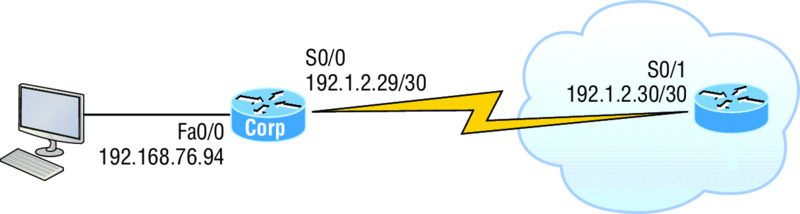
\includegraphics{images/c13f006.jpg}
\caption{{\protect\hyperlink{c13.xhtmlux5cux23figureanchor13-6}{\textbf{FIGURE
13.6}} Last NAT example}}
\end{figure}

By looking at the configured network, use only the following inside
addresses to configure NAT on the Corp router to allow all hosts to
reach the Internet:

\begin{enumerate}
\tightlist
\item
  Inside globals: 198.18.41.129 through 198.18.41.134
\item
  Inside locals: 192.168.76.65 through 192.168.76.94
\end{enumerate}

This one is a bit more challenging because all we have to help us figure
out the configuration is the inside globals and the inside locals. But
even meagerly armed with these crumbs of information, plus the IP
addresses of the router interfaces shown in the figure, we can still
configure this correctly.

To do that, we must first determine what our block sizes are so we can
get our subnet mask for our NAT pool. This will also equip us to
configure the wildcard for the access list.

You should easily be able to see that the block size of the inside
globals is 8 and the block size of the inside locals is 32. Know that
it's critical not to stumble on this foundational information!

So we can configure NAT now that we have our block sizes:

\begin{verbatim}
ip nat pool Corp 198.18.41.129 198.18.41.134 netmask 255.255.255.248
ip nat inside source list 1 pool Corp overload
access-list 1 permit 192.168.76.64 0.0.0.31
\end{verbatim}

Since we had a block of only 8 for our pool, we had to use the
\texttt{overload} command to make sure all 26 hosts can get to the
Internet at the same time.

There is one other simple way to configure NAT, and I use this command
at my home office to connect to my ISP. One command line and it's done!
Here it is:

\begin{verbatim}
ip nat inside source list 1 int s0/0/0 overload
\end{verbatim}

I can't say enough how much I love efficiency, and being able to achieve
something cool using one measly line always makes me happy! My one
little powerfully elegant line essentially says, ``Use my outside local
as my inside global and overload it.'' Nice! Of course, I still had to
create ACL 1 and add the inside and outside interface commands to the
configuration, but this is a really nice, fast way to configure NAT if
you don't have a pool of addresses to use.



\section{Summary}

Now this really was a fun chapter. Come on -- admit it! You learned a lot
about Network Address Translation (NAT) and how it's configured as
static and dynamic as well as with Port Address Translation (PAT), also
called NAT Overload.

I also described how each flavor of NAT is used in a network as well as
how each type is configured.

We finished up by going through some verification and troubleshooting
commands. Now don't forget to practice all the wonderfully helpful labs
until you've got them nailed down tight!



\section{Exam essentials}

\textbf{Understand the term \emph{NAT}.} This may come as news to you,
because I didn't -- okay, failed to -- mention it earlier, but NAT has a
few nicknames. In the industry, it's referred to as network
masquerading, IP-masquerading, and (for those who are besieged with OCD
and compelled to spell everything out) Network Address Translation.
Whatever you want to dub it, basically, they all refer to the process of
rewriting the source/destination addresses of IP packets when they go
through a router or firewall. Just focus on the process that's occurring
and your understanding of it (i.e., the important part) and you're on it
for sure!

\textbf{Remember the three methods of NAT.} The three methods are
static, dynamic, and overloading; the latter is also called PAT.

\textbf{Understand static NAT.} This type of NAT is designed to allow
one-to-one mapping between local and global addresses.

\textbf{Understand dynamic NAT.} This version gives you the ability to
map a range of unregistered IP addresses to a registered IP address from
out of a pool of registered IP addresses.

\textbf{Understand overloading.} Overloading really is a form of dynamic
NAT that maps multiple unregistered IP addresses to a single registered
IP address (many-to-one) by using different ports. It's also known as
\emph{PAT}.



\section{Written lab 13}

In this section, you'll complete the following lab to make sure you've
got the information and concepts contained within it fully dialed in:

Lab 13.1: NAT

You can find the answers to this lab in Appendix A, ``Answers to Written
Labs.''

In this section,
write the answers to the following questions:

\begin{enumerate}
\item
  What type of address translation can use only one address to allow
  thousands of hosts to be translated globally?
\item
  What command can you use to show the NAT translations as they occur on
  your router?
\item
  What command will show you the translation table?
\item
  What command will clear all your NAT entries from the translation
  table?
\item
  An inside local is before or after translation?
\item
  An inside global is before or after translation?
\item
  Which command can be used for troubleshooting and displays a summary
  of the NAT configuration as well as counts of active translation types
  and hits to an existing mapping?
\item
  What commands must be used on your router interfaces before NAT will
  translate addresses?
\item
  In the following output, what type of NAT is being used?

\begin{verbatim}
ip nat pool todd-nat 170.168.10.10 170.168.10.20 netmask 255.255.255.0
\end{verbatim}
\item
  Instead of the \texttt{netmask} command, you can use the
  \_\_\_\_\_\_\_\_\_\_\_\_\_ statement.
\end{enumerate}




\section{Hands-on labs}

I am going to use some basic routers for these labs, but really, almost
any Cisco router will work. Also, you can use the LammleSim IOS version
to run through all the labs in this (and every) chapter in this book.

Here is a list of the labs in this chapter:

\begin{enumerate}
\tightlist
\item
  Lab 13.1: Preparing for NAT
\item
  Lab 13.2: Configuring Dynamic NAT
\item
  Lab 13.3: Configuring PAT
\end{enumerate}

I am going to use the network shown in the following diagram for our
hands-on labs. I highly recommend you connect up some routers and run
through these labs. You will configure NAT on router Lab\_A to translate
the private IP address of 192.168.10.0 to a public address of
171.16.10.0.

\begin{figure}
\centering
%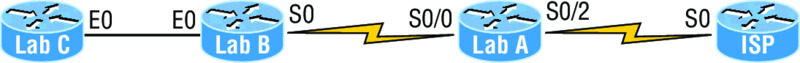
\includegraphics{images/c13f007.jpg}
\caption{}
\end{figure}

\protect\hyperlink{c13.xhtmlux5cux23table13-3}{Table 13.3} shows the
commands we will use and the purpose of each command.



{\protect\hyperlink{c13.xhtmlux5cux23tableanchor13-3}{\textbf{TABLE
13.3}} Command summary for NAT/PAT hands-on labs}

\begin{longtable}[]{@{}ll@{}}
\toprule
Command & Purpose\tabularnewline
\midrule
\endhead
\texttt{ip\ nat\ inside\ source\ list}
\emph{\texttt{acl\ pool}\texttt{name}} & Translates IPs that match the
ACL to the pool\tabularnewline
\texttt{ip\ nat\ inside\ source\ static}
\emph{\texttt{inside\_addr\ outside\_addr}} & Statically maps an inside
local address to an outside global address\tabularnewline
\texttt{ip\ nat\ pool} \emph{\texttt{name}} & Creates an address
pool\tabularnewline
\texttt{ip\ nat\ inside} & Sets an interface to be an inside
interface\tabularnewline
\texttt{ip\ nat\ outside} & Sets an interface to be an outside
interface\tabularnewline
\texttt{show\ ip\ nat\ translations} & Shows current NAT
translations\tabularnewline
\bottomrule
\end{longtable}




\subsection{Lab 13.1: Preparing for NAT}

In this lab, you'll set up your routers with IP addresses and RIP
routing.

\begin{enumerate}
\item
  Configure the routers with the IP addresses listed in the following
  table:

  \begin{longtable}[]{@{}lll@{}}
  \toprule
  \textbf{Router} & \textbf{Interface} & \textbf{IP
  Address}\tabularnewline
  \midrule
  \endhead
  ISP & S0 & 171.16.10.1/24\tabularnewline
  Lab\_A & S0/2 & 171.16.10.2/24\tabularnewline
  Lab\_A & S0/0 & 192.168.20.1/24\tabularnewline
  Lab\_B & S0 & 192.168.20.2/24\tabularnewline
  Lab\_B & E0 & 192.168.30.1/24\tabularnewline
  Lab\_C & E0 & 192.168.30.2/24\tabularnewline
  \bottomrule
  \end{longtable}

  After you configure IP addresses on the routers, you should be able to
  ping from router to router, but since we do not have a routing
  protocol running until the next step, you can verify only from one
  router to another but not through the network until RIP is set up. You
  can use any routing protocol you wish; I am just using RIP for
  simplicity's sake to get this up and running.
\item
  On Lab\_A, configure RIP routing, set a passive interface, and
  configure the default network.

\begin{verbatim}
Lab_A#config t
Lab_A(config)#router rip
Lab_A(config-router)#network 192.168.20.0
Lab_A(config-router)#network 171.16.0.0
Lab_A(config-router)#passive-interface s0/2
Lab_A(config-router)#exit
Lab_A(config)#ip default-network 171.16.10.1
\end{verbatim}

  The \texttt{passive-interface} command stops RIP updates from being
  sent to the ISP and the \texttt{ip\ default-network} command
  advertises a default network to the other routers so they know how to
  get to the Internet.
\item
  On Lab\_B, configure RIP routing:

\begin{verbatim}
Lab_B#config t
Lab_B(config)#router rip
Lab_B(config-router)#network 192.168.30.0
Lab_B(config-router)#network 192.168.20.0
\end{verbatim}
\item
  On Lab\_C, configure RIP routing:

\begin{verbatim}
Lab_C#config t
Lab_C(config)#router rip
Lab_C(config-router)#network 192.168.30.0
\end{verbatim}
\item
  On the ISP router, configure a default route to the corporate network:

\begin{verbatim}
ISP#config t
ISP(config)#ip route 0.0.0.0 0.0.0.0 s0
\end{verbatim}
\item
  Configure the ISP router so you can telnet into the router without
  being prompted for a password:

\begin{verbatim}
ISP#config t
ISP(config)#line vty 0 4
ISP(config-line)#no login
\end{verbatim}
\item
  Verify that you can ping from the ISP router to the Lab\_C router and
  from the Lab\_C router to the ISP router. If you cannot, troubleshoot
  your network.
\end{enumerate}




\subsection{Lab 13.2: Configuring dynamic NAT}

In this lab, you'll configure dynamic NAT on the Lab\_A router.

\begin{enumerate}
\item
  Create a pool of addresses called GlobalNet on the Lab\_A router. The
  pool should contain a range of addresses of 171.16.10.50 through
  171.16.10.55.

\begin{verbatim}
Lab_A(config)#ip nat pool GlobalNet 171.16.10.50 171.16.10.55
net 255.255.255.0
\end{verbatim}
\item
  Create access list
  1. This list permits traffic from the 192.168.20.0 and 192.168.30.0
  network to be translated.

\begin{verbatim}
Lab_A(config)#access-list 1 permit 192.168.20.0 0.0.0.255
Lab_A(config)#access-list 1 permit 192.168.30.0 0.0.0.255
\end{verbatim}
\item
  Map the access list to the pool that was created.

\begin{verbatim}
Lab_A(config)#ip nat inside source list 1 pool GlobalNet
\end{verbatim}
\item
  Configure serial 0/0 as an inside NAT interface.

\begin{verbatim}
Lab_A(config)#int s0/0
Lab_A(config-if)#ip nat inside
\end{verbatim}
\item
  Configure serial 0/2 as an outside NAT interface.

\begin{verbatim}
Lab_A(config-if)#int s0/2
Lab_A(config-if)#ip nat outside
\end{verbatim}
\item
  Move the console connection to the Lab\_C router. Log in to the Lab\_C
  router. Telnet from the Lab\_C router to the ISP router.

\begin{verbatim}
Lab_C#telnet 171.16.10.1
\end{verbatim}
\item
  Move the console connection to the Lab\_B router. Log in to the Lab\_B
  router. Telnet from the Lab\_B router to the ISP router.

\begin{verbatim}
Lab_B#telnet 171.16.10.1
\end{verbatim}
\item
  Execute the command \texttt{show\ users} from the ISP router. (This
  shows who is accessing the VTY lines.)

\begin{verbatim}
ISP#show users
\end{verbatim}

  \begin{enumerate}
  \item
    What does it show as your source IP
    address?\_\_\_\_\_\_\_\_\_\_\_\_\_\_\_\_
  \item
    What is your real source IP
    address?\_\_\_\_\_\_\_\_\_\_\_\_\_\_\_\_\_\_

    The \texttt{show\ users} output should look something like this:

\begin{verbatim}
ISP>sh users
    Line       User       Host(s)              Idle       Location
   0 con 0                idle                 00:03:32
   2 vty 0                idle                 00:01:33 171.16.10.50
*  3 vty 1                idle                 00:00:09 171.16.10.51
  Interface  User      Mode                     Idle Peer Address
ISP>
\end{verbatim}

    \begin{center}\rule{0.5\linewidth}{0.5pt}\end{center}

    
    %\includegraphics{images/note.png}
    Notice
    that there is a one-to-one translation. This means you must have a
    real IP address for every host that wants to get to the Internet,
    which is not typically possible.

    \begin{center}\rule{0.5\linewidth}{0.5pt}\end{center}
  \end{enumerate}
\item
  Leave the session open on the ISP router and connect to Lab\_A. (Use
  \textbf{Ctrl+Shift+6}, let go, and then press \textbf{X}.)
\item
  Log in to your Lab\_A router and view your current translations by
  entering the \texttt{show\ ip\ nat\ translations} command. You should
  see something like this:

\begin{verbatim}
Lab_A#sh ip nat translations
Pro Inside global      Inside local       Outside local      Outside global
--- 171.16.10.50       192.168.30.2       ---                ---
--- 171.16.10.51       192.168.20.2       ---                ---
Lab_A#
\end{verbatim}
\item
  If you turn on \texttt{debug\ ip\ nat} on the Lab\_A router and then
  ping through the router, you will see the actual NAT process take
  place, which will look something like this:

\begin{verbatim}
00:32:47: NAT*: s=192.168.30.2->171.16.10.50, d=171.16.10.1 [5]
00:32:47: NAT*: s=171.16.10.1, d=171.16.10.50->192.168.30.2
\end{verbatim}
\end{enumerate}




\subsection{Lab 13.3: Configuring PAT}

In this lab, you'll configure PAT on the Lab\_A router. We will use PAT
because we don't want a one-to-one translation, which uses just one IP
address for every user on the network.

\begin{enumerate}
\item
  On the Lab\_A router, delete the translation table and remove the
  dynamic NAT pool.

\begin{verbatim}
Lab_A#clear ip nat translations *
Lab_A#config t
Lab_A(config)#no ip nat pool GlobalNet 171.16.10.50
171.16.10.55 netmask 255.255.255.0
Lab_A(config)#no ip nat inside source list 1 pool GlobalNet
\end{verbatim}
\item
  On the Lab\_A router, create a NAT pool with one address called
  Lammle. The pool should contain a single address, 171.16.10.100. Enter
  the following command:

\begin{verbatim}
Lab_A#config t
Lab_A(config)#ip nat pool Lammle 171.16.10.100 171.16.10.100
net 255.255.255.0
\end{verbatim}
\item
  Create access list 2. It should permit networks 192.168.20.0 and
  192.168.30.0 to be translated.

\begin{verbatim}
Lab_A(config)#access-list 2 permit 192.168.20.0 0.0.0.255
Lab_A(config)#access-list 2 permit 192.168.30.0 0.0.0.255
\end{verbatim}
\item
  Map access list 2 to the new pool, allowing PAT to occur by using the
  \texttt{overload} command.

\begin{verbatim}
Lab_A(config)#ip nat inside source list 2 pool Lammle overload
\end{verbatim}
\item
  Log in to the Lab\_C router and telnet to the ISP router; also, log in
  to the Lab\_B router and telnet to the ISP router.
\item
  From the ISP router, use the \texttt{show\ users} command. The output
  should look like this:

\begin{verbatim}
ISP>sh users
    Line       User       Host(s)              Idle       Location
*  0 con 0                idle                 00:00:00
   2 vty 0                idle                 00:00:39 171.16.10.100
   4 vty 2                idle                 00:00:37 171.16.10.100
 
  Interface  User      Mode               Idle Peer Address
 
ISP>
\end{verbatim}
\item
  From the Lab\_A router, use the \texttt{show\ ip\ nat\ translations}
  command.

\begin{verbatim}
Lab_A#sh ip nat translations
Pro Inside global  Inside local  Outside local Outside global
tcp 171.16.10.100:11001 192.168.20.2:11001 171.16.10.1:23    
171.16.10.1:23
tcp 171.16.10.100:11002 192.168.30.2:11002 171.16.10.1:23    
171.16.10.1:23
\end{verbatim}
\item
  Also make sure the \texttt{debug\ ip\ nat} command is on for the
  Lab\_A router. If you ping from the Lab\_C router to the ISP router,
  the output will look like this:

\begin{verbatim}
01:12:36: NAT: s=192.168.30.2->171.16.10.100, d=171.16.10.1 [35]
01:12:36: NAT*: s=171.16.10.1, d=171.16.10.100->192.168.30.2 [35]
01:12:36: NAT*: s=192.168.30.2->171.16.10.100, d=171.16.10.1 [36]
01:12:36: NAT*: s=171.16.10.1, d=171.16.10.100->192.168.30.2 [36]
01:12:36: NAT*: s=192.168.30.2->171.16.10.100, d=171.16.10.1 [37]
01:12:36: NAT*: s=171.16.10.1, d=171.16.10.100->192.168.30.2 [37]
01:12:36: NAT*: s=192.168.30.2->171.16.10.100, d=171.16.10.1 [38]
01:12:36: NAT*: s=171.16.10.1, d=171.16.10.100->192.168.30.2 [38]
01:12:37: NAT*: s=192.168.30.2->171.16.10.100, d=171.16.10.1 [39]
01:12:37: NAT*: s=171.16.10.1, d=171.16.10.100->192.168.30.2 [39]
\end{verbatim}
\end{enumerate}



\section{Review questions}

\begin{center}\rule{0.5\linewidth}{0.5pt}\end{center}


%\includegraphics{images/note.png}
The
following questions are designed to test your understanding of this
chapter's material. For more information on how to get additional
questions, please see \texttt{www.lammle.com/ccna}.

\begin{center}\rule{0.5\linewidth}{0.5pt}\end{center}

You can find the answers to these questions in Appendix B, ``Answers to
Review Questions.''

\begin{enumerate}
\item
  Which of the following are disadvantages of using NAT? (Choose three.)

  \begin{enumerate}
  \tightlist
  \item
    Translation introduces switching path delays.
  \item
    NAT conserves legally registered addresses.
  \item
    NAT causes loss of end-to-end IP traceability.
  \item
    NAT increases flexibility when connecting to the Internet.
  \item
    Certain applications will not function with NAT enabled.
  \item
    NAT reduces address overlap occurrence.
  \end{enumerate}
\item
  Which of the following are advantages of using NAT? (Choose three.)

  \begin{enumerate}
  \tightlist
  \item
    Translation introduces switching path delays.
  \item
    NAT conserves legally registered addresses.
  \item
    NAT causes loss of end-to-end IP traceability.
  \item
    NAT increases flexibility when connecting to the Internet.
  \item
    Certain applications will not function with NAT enabled.
  \item
    NAT remedies address overlap occurrence.
  \end{enumerate}
\item
  Which command will allow you to see real-time translations on your
  router?

  \begin{enumerate}
  \tightlist
  \item
    \texttt{show\ ip\ nat\ translations}
  \item
    \texttt{show\ ip\ nat\ statistics}
  \item
    \texttt{debug\ ip\ nat}
  \item
    \texttt{clear\ ip\ nat\ translations\ *}
  \end{enumerate}
\item
  Which command will show you all the translations active on your
  router?

  \begin{enumerate}
  \tightlist
  \item
    \texttt{show\ ip\ nat\ translations}
  \item
    \texttt{show\ ip\ nat\ statistics}
  \item
    \texttt{debug\ ip\ nat}
  \item
    \texttt{clear\ ip\ nat\ translations\ *}
  \end{enumerate}
\item
  Which command will clear all the translations active on your router?

  \begin{enumerate}
  \tightlist
  \item
    \texttt{show\ ip\ nat\ translations}
  \item
    \texttt{show\ ip\ nat\ statistics}
  \item
    \texttt{debug\ ip\ nat}
  \item
    \texttt{clear\ ip\ nat\ translations\ *}
  \end{enumerate}
\item
  Which command will show you the summary of the NAT configuration?

  \begin{enumerate}
  \tightlist
  \item
    \texttt{show\ ip\ nat\ translations}
  \item
    \texttt{show\ ip\ nat\ statistics}
  \item
    \texttt{debug\ ip\ nat}
  \item
    \texttt{clear\ ip\ nat\ translations\ *}
  \end{enumerate}
\item
  Which command will create a dynamic pool named Todd that will provide
  you with 30 global addresses?

  \begin{enumerate}
  \tightlist
  \item
    \texttt{ip\ nat\ pool\ Todd\ 171.16.10.65\ 171.16.10.94\ net\ 255.255.255.240}
  \item
    \texttt{ip\ nat\ pool\ Todd\ 171.16.10.65\ 171.16.10.94\ net\ 255.255.255.224}
  \item
    \texttt{ip\ nat\ pool\ todd\ 171.16.10.65\ 171.16.10.94\ net\ 255.255.255.224}
  \item
    \texttt{ip\ nat\ pool\ Todd\ 171.16.10.1\ 171.16.10.254\ net\ 255.255.255.0}
  \end{enumerate}
\item
  Which of the following are methods of NAT? (Choose three.)

  \begin{enumerate}
  \tightlist
  \item
    Static
  \item
    IP NAT pool
  \item
    Dynamic
  \item
    NAT double-translation
  \item
    Overload
  \end{enumerate}
\item
  When creating a pool of global addresses, which of the following can
  be used instead of the \texttt{netmask} command?

  \begin{enumerate}
  \tightlist
  \item
    \texttt{/} (slash notation)
  \item
    \texttt{prefix-length}
  \item
    \texttt{no\ mask}
  \item
    \texttt{block-size}
  \end{enumerate}
\item
  Which of the following would be a good starting point for
  troubleshooting if your router is not translating?

  \begin{enumerate}
  \tightlist
  \item
    Reboot.
  \item
    Call Cisco.
  \item
    Check your interfaces for the correct configuration.
  \item
    Run the \texttt{debug\ all} command.
  \end{enumerate}
\item
  Which of the following would be good reasons to run NAT? (Choose
  three.)

  \begin{enumerate}
  \tightlist
  \item
    You need to connect to the Internet and your hosts don't have
    globally unique IP addresses.
  \item
    You change to a new ISP that requires you to renumber your network.
  \item
    You don't want any hosts connecting to the Internet.
  \item
    You require two intranets with duplicate addresses to merge.
  \end{enumerate}
\item
  Which of the
  following is considered to be the inside host's address after
  translation?

  \begin{enumerate}
  \tightlist
  \item
    Inside local
  \item
    Outside local
  \item
    Inside global
  \item
    Outside global
  \end{enumerate}
\item
  Which of the following is considered to be the inside host's address
  before translation?

  \begin{enumerate}
  \tightlist
  \item
    Inside local
  \item
    Outside local
  \item
    Inside global
  \item
    Outside global
  \end{enumerate}
\item
  By looking at the following output, determine which of the following
  commands would allow dynamic translations?

\begin{verbatim}
Router#show ip nat trans
Pro   Inside global   Inside local   Outside local Outside global
---   1.1.128.1       10.1.1.1       ---           ---
---   1.1.130.178     10.1.1.2       ---           ---
---   1.1.129.174     10.1.1.10      ---           ---
---   1.1.130.101     10.1.1.89      ---           ---
---   1.1.134.169     10.1.1.100     ---           ---
---   1.1.135.174     10.1.1.200      ---           ---
\end{verbatim}

  \begin{enumerate}
  \tightlist
  \item
    \texttt{ip\ nat\ inside\ source\ pool\ todd\ 1.1.128.1\ 1.1.135.254\ prefix-length\ 19}
  \item
    \texttt{ip\ nat\ pool\ todd\ 1.1.128.1\ 1.1.135.254\ prefix-length\ 19}
  \item
    \texttt{ip\ nat\ pool\ todd\ 1.1.128.1\ 1.1.135.254\ prefix-length\ 18}
  \item
    \texttt{ip\ nat\ pool\ todd\ 1.1.128.1\ 1.1.135.254\ prefix-length\ 21}
  \end{enumerate}
\item
  Your inside locals are not being translated to the inside global
  addresses. Which of the following commands will show you if your
  inside globals are allowed to use the NAT pool?

\begin{verbatim}
ip nat pool Corp 198.18.41.129 198.18.41.134 netmask 255.255.255.248
ip nat inside source list 100 int s0/0 Corp overload
\end{verbatim}

  \begin{enumerate}
  \tightlist
  \item
    \texttt{debug\ ip\ nat}
  \item
    \texttt{show\ access-list}
  \item
    \texttt{show\ ip\ nat\ translation}
  \item
    \texttt{show\ ip\ nat\ statistics}
  \end{enumerate}
\item
  Which command would
  you place on the interface of a private network?

  \begin{enumerate}
  \tightlist
  \item
    \texttt{ip\ nat\ inside}
  \item
    \texttt{ip\ nat\ outside}
  \item
    \texttt{ip\ outside\ global}
  \item
    \texttt{ip\ inside\ local}
  \end{enumerate}
\item
  Which command would you place on an interface connected to the
  Internet?

  \begin{enumerate}
  \tightlist
  \item
    \texttt{ip\ nat\ inside}
  \item
    \texttt{ip\ nat\ outside}
  \item
    \texttt{ip\ outside\ global}
  \item
    \texttt{ip\ inside\ local}
  \end{enumerate}
\item
  Port Address Translation is also called what?

  \begin{enumerate}
  \tightlist
  \item
    NAT Fast
  \item
    NAT Static
  \item
    NAT Overload
  \item
    Overloading Static
  \end{enumerate}
\item
  What does the asterisk (*) represent in the following output?

\begin{verbatim}
NAT*: s=172.16.2.2, d=192.168.2.1->10.1.1.1 [1]
\end{verbatim}

  \begin{enumerate}
  \tightlist
  \item
    The packet was destined for a local interface on the router.
  \item
    The packet was translated and fast-switched to the destination.
  \item
    The packet attempted to be translated but failed.
  \item
    The packet was translated but there was no response from the remote
    host.
  \end{enumerate}
\item
  Which of the following needs to be added to the configuration to
  enable PAT?

\begin{verbatim}
ip nat pool Corp 198.18.41.129 198.18.41.134 netmask 255.255.255.248
access-list 1 permit 192.168.76.64 0.0.0.31
\end{verbatim}

  \begin{enumerate}
  \tightlist
  \item
    \texttt{ip\ nat\ pool\ inside\ overload}
  \item
    \texttt{ip\ nat\ inside\ source\ list\ 1\ pool\ Corp\ overload}
  \item
    \texttt{ip\ nat\ pool\ outside\ overload}
  \item
    \texttt{ip\ nat\ pool\ Corp\ 198.41.129\ net\ 255.255.255.0\ overload}
  \end{enumerate}
\end{enumerate}






\part{The transport layer}


\part{The data-link layer}

\chapter{Ethernet}

\section{Ethernet}


We have now finished our general discussion of channel allocation
protocols in the abstract, so it is time to see how these principles
apply to real systems, in particular, LANs. As discussed in
\protect\hyperlink{0130661023_ch01lev1sec5.htmlux5cux23ch01lev2sec23}{Sec.
1.5.3}, the IEEE has standardized a number of local area networks and
metropolitan area networks under the name of IEEE 802. A few have
survived but many have not, as we saw in
\protect\hyperlink{0130661023_ch01lev1sec6.htmlux5cux23ch01fig38}{Fig.
1-38}. Some people who believe in reincarnation think that Charles
Darwin came back as a member of the IEEE Standards Association to weed
out the unfit. The most important of the survivors are 802.3 (Ethernet)
and 802.11 (wireless LAN). With 802.15 (Bluetooth) and 802.16 (wireless
MAN), it is too early to tell. Please consult the 5th edition of this
book to find out. Both 802.3 and 802.11 have different physical layers
and different MAC sublayers but converge on the same logical link
control sublayer (defined in 802.2), so they have the same interface to
the network layer.

We introduced Ethernet in
\protect\hyperlink{0130661023_ch01lev1sec5.htmlux5cux23ch01lev2sec23}{Sec.
1.5.3} and will not repeat that material here. Instead we will focus on
the technical details of Ethernet, the protocols, and recent
developments in high-speed (gigabit) Ethernet. Since Ethernet and IEEE
802.3 are identical except for two minor differences that we will
discuss shortly, many people use the terms ''Ethernet'' and ''IEEE
802.3'' interchangeably, and we will do so, too. For more information
about Ethernet, see (Breyer and Riley, 1999 ; Seifert, 1998; and
Spurgeon, 2000).

\subsection{Ethernet cabling}

Since the name ``Ethernet'' refers to the cable (the ether), let us start our discussion there.
Four types of cabling are commonly used, as shown in \cref{fig:common-ethernet-cabling}.


\begin{table}
   \centering
   %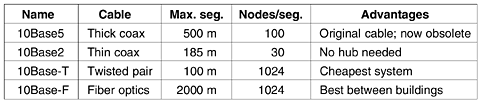
\includegraphics[width=\textwidth]{images/04fig13.png}
   \begin{tabular}{rlrrl}
   \textit{name}     & cable         & max. seg. & nodes/seg. & advantages                   \\[.75ex]
   \textit{10Base5}  & thick coax    &    500\,m &        100 & original cable; now obsolete \\
   \textit{10Base2}  & thin coax     &    185\,m &         30 & no hub needed                \\
   \textit{10Base-T} & twisted pair  &    100\,m &       1024 & cheapest system              \\
   \textit{10Base-F} & fiber optics  &   2000\,m &       1024 & best between buildings       \\
   \end{tabular}
   \caption{The most common kinds of Ethernet cabling.}
   \label{fig:common-ethernet-cabling}
\end{table}


Historically, \emph{10Base5} cabling, popularly called \emph{thick Ethernet}, came first.
It resembles a yellow garden hose, with markings every 2.5~meters to show where the taps go.
(The 802.3 standard does not actually \emph{require} the cable to be yellow, but it does \emph{suggest} it.)
Connections to it are generally made using \emph{vampire taps}, in which a pin is \emph{very} carefully forced halfway into the coaxial cable's core.
The notation 10Base5 means that it operates at 10\,Mbps, uses baseband signaling, and can support segments of up to 500~meters.
The first number is the speed
in Mbps. Then comes the word ``Base'' (or sometimes ``BASE'') to
indicate baseband transmission. There used to be a broadband variant,
10Broad36, but it never caught on in the marketplace and has since
vanished. Finally, if the medium is coax, its length is given rounded to
units of 100\,m after ``Base.''

Historically, the second cable type was \emph{10Base2}, or \emph{thin Ethernet,}
which, in contrast to the garden-hose-like thick Ethernet, bends easily.
Connections to it are made using industry-standard BNC connectors to
form T junctions, rather than using vampire taps. BNC connectors are
easier to use and more reliable. Thin Ethernet is much cheaper and
easier to install, but it can run for only 185~meters per segment, each of which can handle only 30~machines.

Detecting cable breaks, excessive length, bad taps, or loose connectors
can be a major problem with both media. For this reason, techniques have
been developed to track them down. Basically, a pulse of known shape is
injected into the cable. If the pulse hits an obstacle or the end of the
cable, an echo will be generated and sent back. By carefully timing the
interval between sending the pulse and receiving the echo, it is
possible to localize the origin of the echo. This technique is called
\emph{time domain reflectometry}.

The problems associated with finding cable breaks drove systems toward a
different kind of wiring pattern, in which all stations have a cable
running to a central {hub} in which they are all connected electrically
(as if they were soldered together). Usually, these wires are telephone
company twisted pairs, since most office buildings are already wired
this way, and normally plenty of spare pairs are available. This scheme
is called {10Base-T}. Hubs do not buffer incoming traffic. We will
discuss an improved version of this idea (switches), which do buffer
incoming traffic later in this chapter.

These three wiring schemes are illustrated in \cref{fig:three-ethernet-cabling}.
For 10Base5, a {transceiver} is clamped securely around the cable
so that its tap makes contact with the inner core. The transceiver
contains the electronics that handle carrier detection and collision
detection. When a collision is detected, the transceiver also puts a
special invalid signal on the cable to ensure that all other
transceivers also realize that a collision has occurred.


\begin{figure}
   \centering
   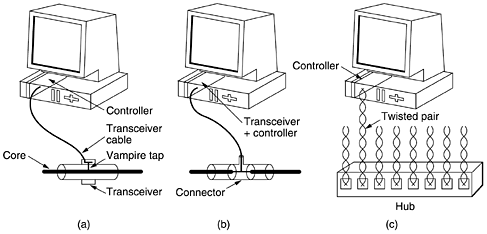
\includegraphics[width=.7\textwidth]{images/04fig14.png}
   \caption{Three kinds of Ethernet cabling. (a) 10Base5. (b) 10Base2. (c) 10Base-T.}
   \label{fig:three-ethernet-cabling}
\end{figure}


With 10Base5, a {transceiver cable} or {drop cable} connects the
transceiver to an interface board in the computer. The transceiver cable
may be up to 50 meters long and contains five individually shielded
twisted pairs. Two of the pairs are for data in and data out,
respectively. Two more are for control signals in and out. The fifth
pair, which is not always used, allows the computer to power the
transceiver electronics. Some transceivers allow up to eight nearby
computers to be attached to them, to reduce the number of transceivers
needed.

The transceiver cable terminates on an interface board inside the
computer. The interface board contains a controller chip that transmits
frames to, and receives frames from, the transceiver. The controller is
responsible for assembling the data into the proper frame format, as
well as computing checksums on outgoing frames and verifying them on
incoming frames. Some controller chips also manage a pool of buffers for
incoming frames, a queue of buffers to be transmitted, direct memory
transfers with the host computers, and other aspects of network
management.

With 10Base2, the connection to the cable is just a passive BNC
T-junction connector. The transceiver electronics are on the controller
board, and each station always has its own transceiver.

With 10Base-T, there is no shared cable at all, just the hub (a box full
of electronics) to which each station is connected by a dedicated (i.e.,
not shared) cable. Adding or removing a station is simpler in this
configuration, and cable breaks can be detected easily. The disadvantage
of 10Base-T is that the maximum cable run from the hub is only 100
meters, maybe 200 meters if very high quality category 5 twisted pairs
are used. Nevertheless, 10Base-T quickly became dominant due to its use
of existing wiring and the ease of maintenance that it offers. A faster
version of 10Base-T (100Base-T) will be discussed later in this chapter.

A fourth cabling option for Ethernet is {10Base-F}, which uses fiber
optics. This alternative is expensive due to the cost of the connectors
and terminators, but it has excellent noise immunity and is the method
of choice when running between buildings or widely-separated hubs. Runs
of up to km are allowed. It also offers good security since wiretapping
fiber is much more difficult than wiretapping copper wire.

\protect\hyperlink{0130661023_ch04lev1sec3.htmlux5cux23ch04fig15}{Figure
4-15} shows different ways of wiring a building. In
\protect\hyperlink{0130661023_ch04lev1sec3.htmlux5cux23ch04fig15}{Fig.
4-15(a)}, a single cable is snaked from room to room, with each station
tapping into it at the nearest point. In
\protect\hyperlink{0130661023_ch04lev1sec3.htmlux5cux23ch04fig15}{Fig.
4-15(b)}, a vertical spine runs from the basement to the roof, with
horizontal cables on each floor connected to the spine by special
amplifiers (repeaters). In some buildings, the horizontal cables are
thin and the backbone is thick. The most general topology is the tree,
as in
\protect\hyperlink{0130661023_ch04lev1sec3.htmlux5cux23ch04fig15}{Fig.
4-15(c)}, because a network with two paths between some pairs of
stations would suffer from interference between the two signals.

\subparagraph[Figure 4-15. Cable topologies. (a) Linear. (b) Spine. (c)
Tree. (d)
Segmented.]{\texorpdfstring{\protect\hypertarget{0130661023_ch04lev1sec3.htmlux5cux23ch04fig15}{}{}Figure
4-15. Cable topologies. (a) Linear. (b) Spine. (c) Tree. (d)
Segmented.}{Figure 4-15. Cable topologies. (a) Linear. (b) Spine. (c) Tree. (d) Segmented.}}

%\includegraphics{04fig15.gif}

Each version of Ethernet has a maximum cable length per segment. To
allow larger networks, multiple cables can be connected by {repeaters},
as shown in
\protect\hyperlink{0130661023_ch04lev1sec3.htmlux5cux23ch04fig15}{Fig.
4-15(d)}. A repeater is a physical layer device. It receives, amplifies
(regenerates), and retransmits signals in both directions. As far as the
software is concerned, a series of cable segments connected by repeaters
is no different from a single cable (except for some delay introduced by
the repeaters). A system may contain multiple cable segments and
multiple repeaters, but no two transceivers may be more than 2.5 km
apart and no path between any two transceivers may traverse more than
four repeaters.

\protect\hypertarget{0130661023_ch04lev1sec3.htmlux5cux23ch04lev2sec10}{}{}

\subsection{Manchester Encoding}

None of the versions of Ethernet uses straight binary encoding with 0
volts for a 0 bit and 5 volts for a 1 bit because it leads to
ambiguities. If one station sends the bit string 0001000, others might
falsely interpret it as 10000000 or 01000000 because they cannot tell
the difference between an idle sender (0 volts) and a 0 bit (0 volts).
This problem can be solved by using +1 volts for a 1 and -1 volts for a
0, but there is still the problem of a receiver sampling the signal at a
slightly different frequency than the sender used to generate it.
Different clock speeds can cause the receiver and sender to get out of
synchronization about where the bit boundaries are, especially after a
long run of consecutive 0s or a long run of consecutive 1s.

What is needed is a way for receivers to unambiguously determine the
start, end, or middle of each bit without reference to an external
clock. Two such approaches are called {Manchester encoding} and
{differential Manchester encoding}. With Manchester encoding, each bit
period is divided into two equal intervals. A binary 1 bit is sent by
having the voltage set high during the first interval and low in the
second one. A binary 0 is just the reverse: first low and then high.
This scheme ensures that every bit period has a transition in the
middle, making it easy for the receiver to synchronize with the sender.
A disadvantage of Manchester encoding is that it requires twice as much
bandwidth as straight binary encoding because the pulses are half the
width. For example, to send data at 10 Mbps, the signal has to change 20
million times/sec. Manchester encoding is shown in
\protect\hyperlink{0130661023_ch04lev1sec3.htmlux5cux23ch04fig16}{Fig.
4-16(b)}.

\subparagraph[Figure 4-16. (a) Binary encoding. (b) Manchester encoding.
(c) Differential Manchester
encoding.]{\texorpdfstring{\protect\hypertarget{0130661023_ch04lev1sec3.htmlux5cux23ch04fig16}{}{}Figure
4-16. (a) Binary encoding. (b) Manchester encoding. (c) Differential
Manchester
encoding.}{Figure 4-16. (a) Binary encoding. (b) Manchester encoding. (c) Differential Manchester encoding.}}

%\includegraphics{04fig16.gif}

Differential Manchester encoding, shown in
\protect\hyperlink{0130661023_ch04lev1sec3.htmlux5cux23ch04fig16}{Fig.
4-16(c)}, is a variation of basic Manchester encoding. In it, a 1 bit is
indicated by the absence of a transition at the start of the interval. A
0 bit is indicated by the presence of a transition at the start of the
interval. In both cases, there is a transition in the middle as well.
The differential scheme requires more complex equipment but offers
better noise immunity. All Ethernet systems use Manchester encoding due
to its simplicity. The high signal is + 0.85 volts and the low signal is
- 0.85 volts, giving a DC value of 0 volts. Ethernet does not use
differential Manchester encoding, but other LANs (e.g., the 802.5 token
ring) do use it.

\protect\hypertarget{0130661023_ch04lev1sec3.htmlux5cux23ch04lev2sec11}{}{}

\subsection{The Ethernet MAC sublayer protocol}

The original DIX (DEC, Intel, Xerox) frame structure is shown in
\protect\hyperlink{0130661023_ch04lev1sec3.htmlux5cux23ch04fig17}{Fig.
4-17(a)}. Each frame starts with a {Preamble} of 8 bytes, each
containing the bit pattern 10101010. The Manchester encoding of this
pattern produces a 10-MHz square wave for 6.4 µsec to allow the
receiver's clock to synchronize with the sender's. They are required to
stay synchronized for the rest of the frame, using the Manchester
encoding to keep track of the bit boundaries.

\subparagraph[Figure 4-17. Frame formats. (a) DIX Ethernet. (b) IEEE
802.3.]{\texorpdfstring{\protect\hypertarget{0130661023_ch04lev1sec3.htmlux5cux23ch04fig17}{}{}Figure
4-17. Frame formats. (a) DIX Ethernet. (b) IEEE
802.3.}{Figure 4-17. Frame formats. (a) DIX Ethernet. (b) IEEE 802.3.}}

%\includegraphics{04fig17.gif}

The frame contains two addresses, one for the destination and one for
the source. The standard allows 2-byte and 6-byte addresses, but the
parameters defined for the 10-Mbps baseband standard use only the 6-byte
addresses. The high-order bit of the destination address is a 0 for
ordinary addresses and 1 for group addresses. Group addresses allow
multiple stations to listen to a single address. When a frame is sent to
a group address, all the stations in the group receive it. Sending to a
group of stations is called {multicast}. The address consisting of all 1
bits is reserved for {broadcast}. A frame containing all 1s in the
destination field is accepted by all stations on the network. The
difference between multicast and broadcast is important enough to
warrant repeating. A multicast frame is sent to a selected group of
stations on the Ethernet; a broadcast frame is sent to all stations on
the Ethernet. Multicast is more selective, but involves group
management. Broadcasting is coarser but does not require any group
management.

Another interesting feature of the addressing is the use of bit 46
(adjacent to the high-order bit) to distinguish local from global
addresses. Local addresses are assigned by each network administrator
and have no significance outside the local network. Global addresses, in
contrast, are assigned centrally by IEEE to ensure that no two stations
anywhere in the world have the same global address. With 48 - 2 = 46
bits available, there are about 7 x 10\textsuperscript{13} global
addresses. The idea is that any station can uniquely address any other
station by just giving the right 48-bit number. It is up to the network
layer to figure out how to locate the destination.

Next comes the {Type} field, which tells the receiver what to do with
the frame. Multiple network-layer protocols may be in use at the same
time on the same machine, so when an Ethernet frame arrives, the kernel
has to know which one to hand the frame to. The {Type} field specifies
which process to give the frame to.

Next come the data, up to 1500 bytes. This limit was chosen somewhat
arbitrarily at the time the DIX standard was cast in stone, mostly based
on the fact that a transceiver needs enough RAM to hold an entire frame
and RAM was expensive in 1978. A larger upper limit would have meant
more RAM, hence a more expensive transceiver.

In addition to there being a maximum frame length, there is also a
minimum frame length. While a data field of 0 bytes is sometimes useful,
it causes a problem. When a transceiver detects a collision, it
truncates the current frame, which means that stray bits and pieces of
frames appear on the cable all the time. To make it easier to
distinguish valid frames from garbage, Ethernet requires that valid
frames must be at least 64 bytes long, from destination address to
checksum, including both. If the data portion of a frame is less than 46
bytes, the {Pad} field is used to fill out the frame to the minimum
size.

Another (and more important) reason for having a minimum length frame is
to prevent a station from completing the transmission of a short frame
before the first bit has even reached the far end of the cable, where it
may collide with another frame. This problem is illustrated in
\protect\hyperlink{0130661023_ch04lev1sec3.htmlux5cux23ch04fig18}{Fig.
4-18}. At time 0, station {A}, at one end of the network, sends off a
frame. Let us call the propagation time for this frame to reach the
other end {t}. Just before the frame gets to the other end (i.e., at
time {t}-{e}), the most distant station, {B}, starts transmitting. When
{B} detects that it is receiving more power than it is putting out, it
knows that a collision has occurred, so it aborts its transmission and
generates a 48-bit noise burst to warn all other stations. In other
words, it jams the ether to make sure the sender does not miss the
collision. At about time 2{t}, the sender sees the noise burst and
aborts its transmission, too. It then waits a random time before trying
again.

\subparagraph[Figure 4-18. Collision detection can take as long as
2{t}.]{\texorpdfstring{\protect\hypertarget{0130661023_ch04lev1sec3.htmlux5cux23ch04fig18}{}{}Figure
4-18. Collision detection can take as long as
2{t}.}{Figure 4-18. Collision detection can take as long as 2t.}}

%\includegraphics{04fig18.gif}

If a station tries to transmit a very short frame, it is conceivable
that a collision occurs, but the transmission completes before the noise
burst gets back at 2{t}. The sender will then incorrectly conclude that
the frame was successfully sent. To prevent this situation from
occurring, all frames must take more than 2{t} to send so that the
transmission is still taking place when the noise burst gets back to the
sender. For a 10-Mbps LAN with a maximum length of 2500 meters and four
repeaters (from the 802.3 specification), the round-trip time (including
time to propagate through the four repeaters) has been determined to be
nearly 50 µsec in the worst case, including the time to pass through the
repeaters, which is most certainly not zero. Therefore, the minimum
frame must take at least this long to transmit. At 10 Mbps, a bit takes
100 nsec, so 500 bits is the smallest frame that is guaranteed to work.
To add some margin of safety, this number was rounded up to 512 bits or
64 bytes. Frames with fewer than 64 bytes are padded out to 64 bytes
with the {Pad} field.

As the network speed goes up, the minimum frame length must go up or the
maximum cable length must come down, proportionally. For a 2500-meter
LAN operating at 1 Gbps, the minimum frame size would have to be 6400
bytes. Alternatively, the minimum frame size could be 640 bytes and the
maximum distance between any two stations 250 meters. These restrictions
are becoming increasingly painful as we move toward multigigabit
networks.

The final Ethernet field is the {Checksum}. It is effectively a 32-bit
hash code of the data. If some data bits are erroneously received (due
to noise on the cable), the checksum will almost certainly be wrong and
the error will be detected. The checksum algorithm is a cyclic
redundancy check (CRC) of the kind discussed in
\protect\hyperlink{0130661023_ch03.htmlux5cux23ch03}{Chap. 3}. It just
does error detection, not forward error correction.

When IEEE standardized Ethernet, the committee made two changes to the
DIX format, as shown in
\protect\hyperlink{0130661023_ch04lev1sec3.htmlux5cux23ch04fig17}{Fig.
4-17(b)}. The first one was to reduce the preamble to 7 bytes and use
the last byte for a {Start of Frame} delimiter, for compatibility with
802.4 and 802.5. The second one was to change the {Type} field into a
{Length} field. Of course, now there was no way for the receiver to
figure out what to do with an incoming frame, but that problem was
handled by the addition of a small header to the data portion itself to
provide this information. We will discuss the format of the data portion
when we come to logical link control later in this chapter.

Unfortunately, by the time 802.3 was published, so much hardware and
software for DIX Ethernet was already in use that few manufacturers and
users were enthusiastic about converting the {Type} field into a
{Length} field. In 1997 IEEE threw in the towel and said that both ways
were fine with it. Fortunately, all the {Type} fields in use before 1997
were greater than 1500. Consequently, any number there less than or
equal to 1500 can be interpreted as {Length}, and any number greater
than 1500 can be interpreted as {Type}. Now IEEE can maintain that
everyone is using its standard and everybody else can keep on doing what
they were already doing without feeling guilty about it.

\protect\hypertarget{0130661023_ch04lev1sec3.htmlux5cux23ch04lev2sec12}{}{}

\subsection{The binary exponential backoff algorithm}

Let us now see how randomization is done when a collision occurs. The
model is that of
\protect\hyperlink{0130661023_ch04lev1sec2.htmlux5cux23ch04fig05}{Fig.
4-5}. After a collision, time is divided into discrete slots whose
length is equal to the worst-case round-trip propagation time on the
ether (2{t}). To accommodate the longest path allowed by Ethernet, the
slot time has been set to 512 bit times, or 51.2 µsec as mentioned
above.

After the first collision, each station waits either 0 or 1 slot times
before trying again. If two stations collide and each one picks the same
random number, they will collide again. After the second collision, each
one picks either 0, 1, 2, or 3 at random and waits that number of slot
times. If a third collision occurs (the probability of this happening is
0.25), then the next time the number of slots to wait is chosen at
random from the interval 0 to 2\textsuperscript{3} - 1.

In general, after {i} collisions, a random number between 0 and
2{\textsuperscript{i}} - 1 is chosen, and that number of slots is
skipped. However, after ten collisions have been reached, the
randomization interval is frozen at a maximum of 1023 slots. After 16
collisions, the controller throws in the towel and reports failure back
to the computer. Further recovery is up to higher layers.

This algorithm, called {binary exponential backoff}, was chosen to
dynamically adapt to the number of stations trying to send. If the
randomization interval for all collisions was 1023, the chance of two
stations colliding for a second time would be negligible, but the
average wait after a collision would be hundreds of slot times,
introducing significant delay. On the other hand, if each station always
delayed for either zero or one slots, then if 100 stations ever tried to
send at once, they would collide over and over until 99 of them picked 1
and the remaining station picked 0. This might take years. By having the
randomization interval grow exponentially as more and more consecutive
collisions occur, the algorithm ensures a low delay when only a few
stations collide but also ensures that the collision is resolved in a
reasonable interval when many stations collide. Truncating the backoff
at 1023 keeps the bound from growing too large.

As described so far, CSMA/CD provides no acknowledgements. Since the
mere absence of collisions does not guarantee that bits were not garbled
by noise spikes on the cable, for reliable communication the destination
must verify the checksum, and if correct, send back an acknowledgement
frame to the source. Normally, this acknowledgement would be just
another frame as far as the protocol is concerned and would have to
fight for channel time just like a data frame. However, a simple
modification to the contention algorithm would allow speedy confirmation
of frame receipt (Tokoro and Tamaru, 1977). All that would be needed is
to reserve the first contention slot following successful transmission
for the destination station. Unfortunately, the standard does not
provide for this possibility.

\protect\hypertarget{0130661023_ch04lev1sec3.htmlux5cux23ch04lev2sec13}{}{}

\subsection{Ethernet performance}

Now let us briefly examine the performance of Ethernet under conditions
of heavy and constant load, that is, {k} stations always ready to
transmit. A rigorous analysis of the binary exponential backoff
algorithm is complicated. Instead, we will follow Metcalfe and Boggs
(1976) and assume a constant retransmission probability in each slot. If
each station transmits during a contention slot with probability {p},
the probability {A} that some station acquires the channel in that slot
is

\textbf{\protect\hypertarget{0130661023_ch04lev1sec3.htmlux5cux23ch04eq05}{}{}
Equation 4}

%\includegraphics{04icon09.gif}

~

{A} is maximized when {p} = 1{/k}, with {A}
%\includegraphics{u2192.gif}
1{/e} as {k}
%\includegraphics{u2192.gif} %\includegraphics{u221e.gif}{.}
The probability that the contention interval has exactly {j} slots in it
is {A}(1 - {A}){\textsuperscript{j}} \textsuperscript{- 1}, so the mean
number of slots per contention is given by

%\includegraphics{04icon10.gif}

~

Since each slot has a duration 2{t}, the mean contention interval, {w},
is 2{t}{/A.} Assuming optimal {p}, the mean number of contention slots
is never more than {e}, so {w} is at most 2{t}{e}
%\includegraphics{u2248.gif} 5.4{t}.

If the mean frame takes {P} sec to transmit, when many stations have
frames to send,

\textbf{\protect\hypertarget{0130661023_ch04lev1sec3.htmlux5cux23ch04eq06}{}{}
Equation 4}

%\includegraphics{04icon11.gif}

~

Here we see where the maximum cable distance between any two stations
enters into the performance figures, giving rise to topologies other
than that of
\protect\hyperlink{0130661023_ch04lev1sec3.htmlux5cux23ch04fig15}{Fig.
4-15(a)}. The longer the cable, the longer the contention interval. This
observation is why the Ethernet standard specifies a maximum cable
length.

It is instructive to formulate
\protect\hyperlink{0130661023_ch04lev1sec3.htmlux5cux23ch04eq06}{Eq.
(4-6)} in terms of the frame length, {F}, the network bandwidth, {B},
the cable length, {L}, and the speed of signal propagation, {c}, for the
optimal case of {e} contention slots per frame. With {P} = {F/B},
\protect\hyperlink{0130661023_ch04lev1sec3.htmlux5cux23ch04eq06}{Eq.
(4-6)} becomes

\textbf{\protect\hypertarget{0130661023_ch04lev1sec3.htmlux5cux23ch04eq07}{}{}
Equation 4}

%\includegraphics{04icon12.gif}

~

When the second term in the denominator is large, network efficiency
will be low. More specifically, increasing network bandwidth or distance
(the {BL} product) reduces efficiency for a given frame size.
Unfortunately, much research on network hardware is aimed precisely at
increasing this product. People want high bandwidth over long distances
(fiber optic MANs, for example), which suggests that Ethernet
implemented in this manner may not be the best system for these
applications. We will see other ways of implementing Ethernet when we
come to switched Ethernet later in this chapter.

In
\protect\hyperlink{0130661023_ch04lev1sec3.htmlux5cux23ch04fig19}{Fig.
4-19}, the channel efficiency is plotted versus number of ready stations
for 2{t}=51.2 µsec and a data rate of 10 Mbps, using
\protect\hyperlink{0130661023_ch04lev1sec3.htmlux5cux23ch04eq07}{Eq.
(4-7)}. With a 64-byte slot time, it is not surprising that 64-byte
frames are not efficient. On the other hand, with 1024-byte frames and
an asymptotic value of {e} 64-byte slots per contention interval, the
contention period is 174 bytes long and the efficiency is 0.85.

\subparagraph[Figure 4-19. Efficiency of Ethernet at 10 Mbps with
512-bit slot
times.]{\texorpdfstring{\protect\hypertarget{0130661023_ch04lev1sec3.htmlux5cux23ch04fig19}{}{}Figure
4-19. Efficiency of Ethernet at 10 Mbps with 512-bit slot
times.}{Figure 4-19. Efficiency of Ethernet at 10 Mbps with 512-bit slot times.}}

%\includegraphics{04fig19.gif}

To determine the mean number of stations ready to transmit under
conditions of high load, we can use the following (crude) observation.
Each frame ties up the channel for one contention period and one frame
transmission time, for a total of {P} + {w} sec. The number of frames
per second is therefore 1{/}({P} + {w}){.} If each station generates
frames at a mean rate of {l} frames/sec, then when the system is in
state {k}, the total input rate of all unblocked stations combined is
{k}{l} frames/sec. Since in equilibrium the input and output rates must
be identical, we can equate these two expressions and solve for {k.}
(Notice that {w} is a function of {k.}) A more sophisticated analysis is
given in (Bertsekas and Gallager, 1992).

It is probably worth mentioning that there has been a large amount of
theoretical performance analysis of Ethernet (and other networks).
Virtually all of this work has assumed that traffic is Poisson. As
researchers have begun looking at real data, it now appears that network
traffic is rarely Poisson, but self-similar (Paxson and Floyd, 1994; and
Willinger et al., 1995). What this means is that averaging over long
periods of time does not smooth out the traffic. The average number of
frames in each minute of an hour has as much variance as the average
number of frames in each second of a minute. The consequence of this
discovery is that most models of network traffic do not apply to the
real world and should be taken with a grain (or better yet, a metric
ton) of salt.

\protect\hypertarget{0130661023_ch04lev1sec3.htmlux5cux23ch04lev2sec14}{}{}

\subsection{Switched Ethernet}

As more and more stations are added to an Ethernet, the traffic will go
up. Eventually, the LAN will saturate. One way out is to go to a higher
speed, say, from 10 Mbps to 100 Mbps. But with the growth of multimedia,
even a 100-Mbps or 1-Gbps Ethernet can become saturated.

Fortunately, there is an additional way to deal with increased load:
switched Ethernet, as shown in
\protect\hyperlink{0130661023_ch04lev1sec3.htmlux5cux23ch04fig20}{Fig.
4-20}. The heart of this system is a {switch} containing a high-speed
backplane and room for typically 4 to 32 plug-in line cards, each
containing one to eight connectors. Most often, each connector has a
10Base-T twisted pair connection to a single host computer.

\subparagraph[Figure 4-20. A simple example of switched
Ethernet.]{\texorpdfstring{\protect\hypertarget{0130661023_ch04lev1sec3.htmlux5cux23ch04fig20}{}{}Figure
4-20. A simple example of switched
Ethernet.}{Figure 4-20. A simple example of switched Ethernet.}}

%\includegraphics{04fig20.gif}

When a station wants to transmit an Ethernet frame, it outputs a
standard frame to the switch. The plug-in card getting the frame may
check to see if it is destined for one of the other stations connected
to the same card. If so, the frame is copied there. If not, the frame is
sent over the high-speed backplane to the destination station's card.
The backplane typically runs at many Gbps, using a proprietary protocol.

What happens if two machines attached to the same plug-in card transmit
frames at the same time? It depends on how the card has been
constructed. One possibility is for all the ports on the card to be
wired together to form a local on-card LAN. Collisions on this on-card
LAN will be detected and handled the same as any other collisions on a
CSMA/CD network -- with retransmissions using the binary exponential
backoff algorithm. With this kind of plug-in card, only one transmission
per card is possible at any instant, but all the cards can be
transmitting in parallel. With this design, each card forms its own
{collision domain}, independent of the others. With only one station per
collision domain, collisions are impossible and performance is improved.

With the other kind of plug-in card, each input port is buffered, so
incoming frames are stored in the card's on-board RAM as they arrive.
This design allows all input ports to receive (and transmit) frames at
the same time, for parallel, full-duplex operation, something not
possible with CSMA/CD on a single channel. Once a frame has been
completely received, the card can then check to see if the frame is
destined for another port on the same card or for a distant port. In the
former case, it can be transmitted directly to the destination. In the
latter case, it must be transmitted over the backplane to the proper
card. With this design, each port is a separate collision domain, so
collisions do not occur. The total system throughput can often be
increased by an order of magnitude over 10Base5, which has a single
collision domain for the entire system.

Since the switch just expects standard Ethernet frames on each input
port, it is possible to use some of the ports as concentrators. In
\protect\hyperlink{0130661023_ch04lev1sec3.htmlux5cux23ch04fig20}{Fig.
4-20}, the port in the upper-right corner is connected not to a single
station, but to a 12-port hub. As frames arrive at the hub, they contend
for the ether in the usual way, including collisions and binary backoff.
Successful frames make it to the switch and are treated there like any
other incoming frames: they are switched to the correct output line over
the high-speed backplane. Hubs are cheaper than switches, but due to
falling switch prices, they are rapidly becoming obsolete. Nevertheless,
legacy hubs still exist.

\protect\hypertarget{0130661023_ch04lev1sec3.htmlux5cux23ch04lev2sec15}{}{}

\subsection{Fast Ethernet}

At first, 10 Mbps seemed like heaven, just as 1200-bps modems seemed
like heaven to the early users of 300-bps acoustic modems. But the
novelty wore off quickly. As a kind of corollary to Parkinson's Law
(''Work expands to fill the time available for its completion''), it
seemed that data expanded to fill the bandwidth available for their
transmission. To pump up the speed, various industry groups proposed two
new ring-based optical LANs. One was called {FDDI} ({Fiber Distributed
Data Interface}) and the other was called {Fibre Channel}
%\textsuperscript{\protect\hyperlink{0130661023_ch04lev1sec3.htmlux5cux23ch04footnote01}{{[}%\includegraphics{u2020.gif}{]}}}.
To make a long story short, while both were used as backbone networks,
neither one made the breakthrough to the desktop. In both cases, the
station management was too complicated, which led to complex chips and
high prices. The lesson that should have been learned here was KISS
(Keep It Simple, Stupid).

\begin{quote}
%\textsuperscript{\protect\hypertarget{0130661023_ch04lev1sec3.htmlux5cux23ch04footnote01}{}{{[}%\includegraphics{u2020.gif}{]}}}
It is called ''fibre channel'' and not ''fiber channel'' because the
document editor was British.
\end{quote}

In any event, the failure of the optical LANs to catch fire left a gap
for garden-variety Ethernet at speeds above 10 Mbps. Many installations
needed more bandwidth and thus had numerous 10-Mbps LANs connected by a
maze of repeaters, bridges, routers, and gateways, although to the
network managers it sometimes felt that they were being held together by
bubble gum and chicken wire.

It was in this environment that IEEE reconvened the 802.3 committee in
1992 with instructions to come up with a faster LAN. One proposal was to
keep 802.3 exactly as it was, but just make it go faster. Another
proposal was to redo it totally to give it lots of new features, such as
real-time traffic and digitized voice, but just keep the old name (for
marketing reasons). After some wrangling, the committee decided to keep
802.3 the way it was, but just make it go faster. The people behind the
losing proposal did what any computer-industry people would have done
under these circumstances -- they stomped off and formed their own
committee and standardized their LAN anyway (eventually as 802.12). It
flopped miserably.

The 802.3 committee decided to go with a souped-up Ethernet for three
primary reasons:

{}

\begin{enumerate}
\def\labelenumi{\arabic{enumi}.}
\item
  {}

  The need to be backward compatible with existing Ethernet LANs.
\end{enumerate}

{}

The fear that a new protocol might have unforeseen problems.

{}

The desire to get the job done before the technology changed.

The work was done quickly (by standards committees' norms), and the
result, {802.3u}, was officially approved by IEEE in June 1995.
Technically, 802.3u is not a new standard, but an addendum to the
existing 802.3 standard (to emphasize its backward compatibility). Since
practically everyone calls it {fast Ethernet}, rather than 802.3u, we
will do that, too.

The basic idea behind fast Ethernet was simple: keep all the old frame
formats, interfaces, and procedural rules, but just reduce the bit time
from 100 nsec to 10 nsec. Technically, it would have been possible to
copy either 10Base-5 or 10Base-2 and still detect collisions on time by
just reducing the maximum cable length by a factor of ten. However, the
advantages of 10Base-T wiring were so overwhelming that fast Ethernet is
based entirely on this design. Thus, all fast Ethernet systems use hubs
and switches; multidrop cables with vampire taps or BNC connectors are
not permitted.

Nevertheless, some choices still had to be made, the most important
being which wire types to support. One contender was category 3 twisted
pair. The argument for it was that practically every office in the
Western world has at least four category 3 (or better) twisted pairs
running from it to a telephone wiring closet within 100 meters.
Sometimes two such cables exist. Thus, using category 3 twisted pair
would make it possible to wire up desktop computers using fast Ethernet
without having to rewire the building, an enormous advantage for many
organizations.

The main disadvantage of category 3 twisted pair is its inability to
carry 200 megabaud signals (100 Mbps with Manchester encoding) 100
meters, the maximum computer-to-hub distance specified for 10Base-T (see
\protect\hyperlink{0130661023_ch04lev1sec3.htmlux5cux23ch04fig13}{Fig.
4-13}). In contrast, category 5 twisted pair wiring can handle 100
meters easily, and fiber can go much farther. The compromise chosen was
to allow all three possibilities, as shown in
\protect\hyperlink{0130661023_ch04lev1sec3.htmlux5cux23ch04fig21}{Fig.
4-21}, but to pep up the category 3 solution to give it the additional
carrying capacity needed.

\subparagraph[Figure 4-21. The original fast Ethernet
cabling.]{\texorpdfstring{\protect\hypertarget{0130661023_ch04lev1sec3.htmlux5cux23ch04fig21}{}{}Figure
4-21. The original fast Ethernet
cabling.}{Figure 4-21. The original fast Ethernet cabling.}}

%\includegraphics{04fig21.gif}

The category 3 UTP scheme, called {100Base-T4}, uses a signaling speed
of 25 MHz, only 25 percent faster than standard Ethernet's 20 MHz
(remember that Manchester encoding, as shown in
\protect\hyperlink{0130661023_ch04lev1sec3.htmlux5cux23ch04fig16}{Fig.
4-16}, requires two clock periods for each of the 10 million bits each
second). However, to achieve the necessary bandwidth, 100Base-T4
requires four twisted pairs. Since standard telephone wiring for decades
has had four twisted pairs per cable, most offices are able to handle
this. Of course, it means giving up your office telephone, but that is
surely a small price to pay for faster e-mail.

Of the four twisted pairs, one is always to the hub, one is always from
the hub, and the other two are switchable to the current transmission
direction. To get the necessary bandwidth, Manchester encoding is not
used, but with modern clocks and such short distances, it is no longer
needed. In addition, ternary signals are sent, so that during a single
clock period the wire can contain a 0, a 1, or a 2. With three twisted
pairs going in the forward direction and ternary signaling, any one of
27 possible symbols can be transmitted, making it possible to send 4
bits with some redundancy. Transmitting 4 bits in each of the 25 million
clock cycles per second gives the necessary 100 Mbps. In addition, there
is always a 33.3-Mbps reverse channel using the remaining twisted pair.
This scheme, known as {8B/6T} (8 bits map to 6 trits), is not likely to
win any prizes for elegance, but it works with the existing wiring
plant.

For category 5 wiring, the design, {100Base-TX}, is simpler because the
wires can handle clock rates of 125 MHz. Only two twisted pairs per
station are used, one to the hub and one from it. Straight binary coding
is not used; instead a scheme called used{4B/5B}is It is taken from FDDI
and compatible with it. Every group of five clock periods, each
containing one of two signal values, yields 32 combinations. Sixteen of
these combinations are used to transmit the four bit groups 0000, 0001,
0010, ..., 1111. Some of the remaining 16 are used for control purposes
such as marking frames boundaries. The combinations used have been
carefully chosen to provide enough transitions to maintain clock
synchronization. The 100Base-TX system is full duplex; stations can
transmit at 100 Mbps and receive at 100 Mbps at the same time. Often
100Base-TX and 100Base-T4 are collectively referred to as {100Base-T}.

The last option, {100Base-FX}, uses two strands of multimode fiber, one
for each direction, so it, too, is full duplex with 100 Mbps in each
direction. In addition, the distance between a station and the hub can
be up to 2 km.

In response to popular demand, in 1997 the 802 committee added a new
cabling type, 100Base-T2, allowing fast Ethernet to run over two pairs
of existing category 3 wiring. However, a sophisticated digital signal
processor is needed to handle the encoding scheme required, making this
option fairly expensive. So far, it is rarely used due to its
complexity, cost, and the fact that many office buildings have already
been rewired with category 5 UTP.

Two kinds of interconnection devices are possible with 100Base-T: hubs
and switches, as shown in
\protect\hyperlink{0130661023_ch04lev1sec3.htmlux5cux23ch04fig20}{Fig.
4-20}. In a hub, all the incoming lines (or at least all the lines
arriving at one plug-in card) are logically connected, forming a single
collision domain. All the standard rules, including the binary
exponential backoff algorithm, apply, so the system works just like
old-fashioned Ethernet. In particular, only one station at a time can be
transmitting. In other words, hubs require half-duplex communication.

In a switch, each incoming frame is buffered on a plug-in line card and
passed over a high-speed backplane from the source card to the
destination card if need be. The backplane has not been standardized,
nor does it need to be, since it is entirely hidden deep inside the
switch. If past experience is any guide, switch vendors will compete
vigorously to produce ever faster backplanes in order to improve system
throughput. Because 100Base-FX cables are too long for the normal
Ethernet collision algorithm, they must be connected to switches, so
each one is a collision domain unto itself. Hubs are not permitted with
100Base-FX.

As a final note, virtually all switches can handle a mix of 10-Mbps and
100-Mbps stations, to make upgrading easier. As a site acquires more and
more 100-Mbps workstations, all it has to do is buy the necessary number
of new line cards and insert them into the switch. In fact, the standard
itself provides a way for two stations to automatically negotiate the
optimum speed (10 or 100 Mbps) and duplexity (half or full). Most fast
Ethernet products use this feature to autoconfigure themselves.

\protect\hypertarget{0130661023_ch04lev1sec3.htmlux5cux23ch04lev2sec16}{}{}

\subsection{Gigabit Ethernet}

The ink was barely dry on the fast Ethernet standard when the 802
committee began working on a yet faster Ethernet (1995). It was quickly
dubbed {gigabit Ethernet} and was ratified by IEEE in 1998 under the
name 802.3z. This identifier suggests that gigabit Ethernet is going to
be the end of the line unless somebody quickly invents a new letter
after z. Below we will discuss some of the key features of gigabit
Ethernet. More information can be found in (Seifert, 1998).

The 802.3z committee's goals were essentially the same as the 802.3u
committee's goals: make Ethernet go 10 times faster yet remain backward
compatible with all existing Ethernet standards. In particular, gigabit
Ethernet had to offer unacknowledged datagram service with both unicast
and multicast, use the same 48-bit addressing scheme already in use, and
maintain the same frame format, including the minimum and maximum frame
sizes. The final standard met all these goals.

All configurations of gigabit Ethernet are point-to-point rather than
multidrop as in the original 10 Mbps standard, now honored as {classic
Ethernet}. In the simplest gigabit Ethernet configuration, illustrated
in
\protect\hyperlink{0130661023_ch04lev1sec3.htmlux5cux23ch04fig22}{Fig.
4-22(a)}, two computers are directly connected to each other. The more
common case, however, is having a switch or a hub connected to multiple
computers and possibly additional switches or hubs, as shown in
\protect\hyperlink{0130661023_ch04lev1sec3.htmlux5cux23ch04fig22}{Fig.
4-22(b)}. In both configurations each individual Ethernet cable has
exactly two devices on it, no more and no fewer.

\subparagraph[Figure 4-22. (a) A two-station Ethernet. (b) A
multistation
Ethernet.]{\texorpdfstring{\protect\hypertarget{0130661023_ch04lev1sec3.htmlux5cux23ch04fig22}{}{}Figure
4-22. (a) A two-station Ethernet. (b) A multistation
Ethernet.}{Figure 4-22. (a) A two-station Ethernet. (b) A multistation Ethernet.}}

%\includegraphics{04fig22.gif}

Gigabit Ethernet supports two different modes of operation: full-duplex
mode and half-duplex mode. The ''normal'' mode is full-duplex mode,
which allows traffic in both directions at the same time. This mode is
used when there is a central switch connected to computers (or other
switches) on the periphery. In this configuration, all lines are
buffered so each computer and switch is free to send frames whenever it
wants to. The sender does not have to sense the channel to see if
anybody else is using it because contention is impossible. On the line
between a computer and a switch, the computer is the only possible
sender on that line to the switch and the transmission succeeds even if
the switch is currently sending a frame to the computer (because the
line is full duplex). Since no contention is possible, the CSMA/CD
protocol is not used, so the maximum length of the cable is determined
by signal strength issues rather than by how long it takes for a noise
burst to propagate back to the sender in the worst case. Switches are
free to mix and match speeds. Autoconfiguration is supported just as in
fast Ethernet.

The other mode of operation, half-duplex, is used when the computers are
connected to a hub rather than a switch. A hub does not buffer incoming
frames. Instead, it electrically connects all the lines internally,
simulating the multidrop cable used in classic Ethernet. In this mode,
collisions are possible, so the standard CSMA/CD protocol is required.
Because a minimum (i.e., 64-byte) frame can now be transmitted 100 times
faster than in classic Ethernet, the maximum distance is 100 times less,
or 25 meters, to maintain the essential property that the sender is
still transmitting when the noise burst gets back to it, even in the
worst case. With a 2500-meter-long cable, the sender of a 64-byte frame
at 1 Gbps would be long done before the frame got even a tenth of the
way to the other end, let alone to the end and back.

The 802.3z committee considered a radius of 25 meters to be unacceptable
and added two features to the standard to increase the radius. The first
feature, called {carrier extension}, essentially tells the hardware to
add its own padding after the normal frame to extend the frame to 512
bytes. Since this padding is added by the sending hardware and removed
by the receiving hardware, the software is unaware of it, meaning that
no changes are needed to existing software. Of course, using 512 bytes
worth of bandwidth to transmit 46 bytes of user data (the payload of a
64-byte frame) has a line efficiency of 9\%.

The second feature, called {frame bursting}, allows a sender to transmit
a concatenated sequence of multiple frames in a single transmission. If
the total burst is less than 512 bytes, the hardware pads it again. If
enough frames are waiting for transmission, this scheme is highly
efficient and preferred over carrier extension. These new features
extend the radius of the network to 200 meters, which is probably enough
for most offices.

In all fairness, it is hard to imagine an organization going to the
trouble of buying and installing gigabit Ethernet cards to get high
performance and then connecting the computers with a hub to simulate
classic Ethernet with all its collisions. While hubs are somewhat
cheaper than switches, gigabit Ethernet interface cards are still
relatively expensive. To then economize by buying a cheap hub and slash
the performance of the new system is foolish. Still, backward
compatibility is sacred in the computer industry, so the 802.3z
committee was required to put it in.

Gigabit Ethernet supports both copper and fiber cabling, as listed in
\protect\hyperlink{0130661023_ch04lev1sec3.htmlux5cux23ch04fig23}{Fig.
4-23}. Signaling at or near 1 Gbps over fiber means that the light
source has to be turned on and off in under 1 nsec. LEDs simply cannot
operate this fast, so lasers are required. Two wavelengths are
permitted: 0.85 microns (Short) and 1.3 microns (Long). Lasers at 0.85
microns are cheaper but do not work on single-mode fiber.

\subparagraph[Figure 4-23. Gigabit Ethernet
cabling.]{\texorpdfstring{\protect\hypertarget{0130661023_ch04lev1sec3.htmlux5cux23ch04fig23}{}{}Figure
4-23. Gigabit Ethernet
cabling.}{Figure 4-23. Gigabit Ethernet cabling.}}

%\includegraphics{04fig23.gif}

Three fiber diameters are permitted: 10, 50, and 62.5 microns. The first
is for single mode and the last two are for multimode. Not all six
combinations are allowed, however, and the maximum distance depends on
the combination used. The numbers given in
\protect\hyperlink{0130661023_ch04lev1sec3.htmlux5cux23ch04fig23}{Fig.
4-23} are for the best case. In particular, 5000 meters is only
achievable with 1.3 micron lasers operating over 10 micron fiber in
single mode, but this is the best choice for campus backbones and is
expected to be popular, despite its being the most expensive choice.

The 1000Base-CX option uses short shielded copper cables. Its problem is
that it is competing with high-performance fiber from above and cheap
UTP from below. It is unlikely to be used much, if at all.

The last option is bundles of four category 5 UTP wires working
together. Because so much of this wiring is already installed, it is
likely to be the poor man's gigabit Ethernet.

Gigabit Ethernet uses new encoding rules on the fibers. Manchester
encoding at 1 Gbps would require a 2 Gbaud signal, which was considered
too difficult and also too wasteful of bandwidth. Instead a new scheme,
called {8B/10B}, was chosen, based on fibre channel. Each 8-bit byte is
encoded on the fiber as 10 bits, hence the name 8B/10B. Since there are
1024 possible output codewords for each input byte, some leeway was
available in choosing which codewords to allow. The following two rules
were used in making the choices:

{}

\begin{enumerate}
\def\labelenumi{\arabic{enumi}.}
\item
  {}

  No codeword may have more than four identical bits in a row.
\end{enumerate}

{}

No codeword may have more than six 0s or six 1s.

These choices were made to keep enough transitions in the stream to make
sure the receiver stays in sync with the sender and also to keep the
number of 0s and 1s on the fiber as close to equal as possible. In
addition, many input bytes have two possible codewords assigned to them.
When the encoder has a choice of codewords, it always chooses the
codeword that moves in the direction of equalizing the number of 0s and
1s transmitted so far. This emphasis of balancing 0s and 1s is needed to
keep the DC component of the signal as low as possible to allow it to
pass through transformers unmodified. While computer scientists are not
fond of having the properties of transformers dictate their coding
schemes, life is like that sometimes.

Gigabit Ethernets using 1000Base-T use a different encoding scheme since
clocking data onto copper wire in 1 nsec is too difficult. This solution
uses four category 5 twisted pairs to allow four symbols to be
transmitted in parallel. Each symbol is encoded using one of five
voltage levels. This scheme allows a single symbol to encode 00, 01, 10,
11, or a special value for control purposes. Thus, there are 2 data bits
per twisted pair or 8 data bits per clock cycle. The clock runs at 125
MHz, allowing 1-Gbps operation. The reason for allowing five voltage
levels instead of four is to have combinations left over for framing and
control purposes.

A speed of 1 Gbps is quite fast. For example, if a receiver is busy with
some other task for even 1 msec and does not empty the input buffer on
some line, up to 1953 frames may have accumulated there in that 1 ms
gap. Also, when a computer on a gigabit Ethernet is shipping data down
the line to a computer on a classic Ethernet, buffer overruns are very
likely. As a consequence of these two observations, gigabit Ethernet
supports flow control (as does fast Ethernet, although the two are
different).

The flow control consists of one end sending a special control frame to
the other end telling it to pause for some period of time. Control
frames are normal Ethernet frames containing a type of 0x8808. The first
two bytes of the data field give the command; succeeding bytes provide
the parameters, if any. For flow control, PAUSE frames are used, with
the parameter telling how long to pause, in units of the minimum frame
time. For gigabit Ethernet, the time unit is 512 nsec, allowing for
pauses as long as 33.6 msec.

As soon as gigabit Ethernet was standardized, the 802 committee got
bored and wanted to get back to work. IEEE told them to start on
10-gigabit Ethernet. After searching hard for a letter to follow z, they
abandoned that approach and went over to two-letter suffixes. They got
to work and that standard was approved by IEEE in 2002 as 802.3ae. Can
100-gigabit Ethernet be far behind?

\protect\hypertarget{0130661023_ch04lev1sec3.htmlux5cux23ch04lev2sec17}{}{}

\subsection{IEEE 802.2: Logical Link Control}

It is now perhaps time to step back and compare what we have learned in
this chapter with what we studied in the previous one. In
\protect\hyperlink{0130661023_ch03.htmlux5cux23ch03}{Chap. 3}, we saw
how two machines could communicate reliably over an unreliable line by
using various data link protocols. These protocols provided error
control (using acknowledgements) and flow control (using a sliding
window).

In contrast, in this chapter, we have not said a word about reliable
communication. All that Ethernet and the other 802 protocols offer is a
best-efforts datagram service. Sometimes, this service is adequate. For
example, for transporting IP packets, no guarantees are required or even
expected. An IP packet can just be inserted into an 802 payload field
and sent on its way. If it gets lost, so be it.

Nevertheless, there are also systems in which an error-controlled,
flow-controlled data link protocol is desired. IEEE has defined one that
can run on top of Ethernet and the other 802 protocols. In addition,
this protocol, called {LLC} ({Logical Link Control}), hides the
differences between the various kinds of 802 networks by providing a
single format and interface to the network layer. This format,
interface, and protocol are all closely based on the HDLC protocol we
studied in \protect\hyperlink{0130661023_ch03.htmlux5cux23ch03}{Chap.
3}. LLC forms the upper half of the data link layer, with the MAC
sublayer below it, as shown in
\protect\hyperlink{0130661023_ch04lev1sec3.htmlux5cux23ch04fig24}{Fig.
4-24}.

\subparagraph[Figure 4-24. (a) Position of LLC. (b) Protocol
formats.]{\texorpdfstring{\protect\hypertarget{0130661023_ch04lev1sec3.htmlux5cux23ch04fig24}{}{}Figure
4-24. (a) Position of LLC. (b) Protocol
formats.}{Figure 4-24. (a) Position of LLC. (b) Protocol formats.}}

%\includegraphics{04fig24.gif}

Typical usage of LLC is as follows. The network layer on the sending
machine passes a packet to LLC, using the LLC access primitives. The LLC
sublayer then adds an LLC header, containing sequence and
acknowledgement numbers. The resulting structure is then inserted into
the payload field of an 802 frame and transmitted. At the receiver, the
reverse process takes place.

LLC provides three service options: unreliable datagram service,
acknowledged datagram service, and reliable connection-oriented service.
The LLC header contains three fields: a destination access point, a
source access point, and a control field. The access points tell which
process the frame came from and where it is to be delivered, replacing
the DIX {Type} field. The control field contains sequence and
acknowledgement numbers, very much in the style of HDLC (see
\protect\hyperlink{0130661023_ch03lev1sec6.htmlux5cux23ch03fig24}{Fig.
3-24}), but not identical to it. These fields are primarily used when a
reliable connection is needed at the data link level, in which case
protocols similar to the ones discussed in
\protect\hyperlink{0130661023_ch03.htmlux5cux23ch03}{Chap. 3} would be
used. For the Internet, best-efforts attempts to deliver IP packets is
sufficient, so no acknowledgements at the LLC level are required.

\protect\hypertarget{0130661023_ch04lev1sec3.htmlux5cux23ch04lev2sec18}{}{}

\subsection{Retrospective on Ethernet}

Ethernet has been around for over 20 years and has no serious
competitors in sight, so it is likely to be around for many years to
come. Few CPU architectures, operating systems, or programming languages
have been king of the mountain for two decades going on three. Clearly,
Ethernet did something right. What?

Probably the main reason for its longevity is that Ethernet is simple
and flexible. In practice, simple translates into reliable, cheap, and
easy to maintain. Once the vampire taps were replaced by BNC connectors,
failures became extremely rare. People hesitate to replace something
that works perfectly all the time, especially when they know that an
awful lot of things in the computer industry work very poorly, so that
many so-called ''upgrades'' are appreciably worse than what they
replaced.

Simple also translates into cheap. Thin Ethernet and twisted pair wiring
is relatively inexpensive. The interface cards are also low cost. Only
when hubs and switches were introduced were substantial investments
required, but by the time they were in the picture, Ethernet was already
well established.

Ethernet is easy to maintain. There is no software to install (other
than the drivers) and there are no configuration tables to manage (and
get wrong). Also, adding new hosts is as simple as just plugging them
in.

Another point is that Ethernet interworks easily with TCP/IP, which has
become dominant. IP is a connectionless protocol, so it fits perfectly
with Ethernet, which is also connectionless. IP fits much less well with
ATM, which is connection oriented. This mismatch definitely hurt ATM's
chances.

Lastly, Ethernet has been able to evolve in certain crucial ways. Speeds
have gone up by several orders of magnitude and hubs and switches have
been introduced, but these changes have not required changing the
software. When a network salesman shows up at a large installation and
says: ''I have this fantastic new network for you. All you have to do is
throw out all your hardware and rewrite all your software,'' he has a
problem. FDDI, Fibre Channel, and ATM were all faster than Ethernet when
introduced, but they were incompatible with Ethernet, far more complex,
and harder to manage. Eventually, Ethernet caught up with them in terms
of speed, so they had no advantages left and quietly died off except for
ATM's use deep within the core of the telephone system.



% Lammle, ch. 11
\chapter{VLANs and inter-VLAN routing}
\label{chap:lammle-ch11}

I know I keep telling you this, but so you never forget it, here I go, one last time: By default, switches break up collision domains and routers break up broadcast domains.
Okay, I feel better! Now we can move on.

In contrast to the networks of yesterday that were based on collapsed
backbones, today's network design is characterized by a flatter
architecture -- thanks to switches. So now what? How do we break up
broadcast domains in a pure switched internetwork? By creating virtual
local area networks (VLANs). A VLAN is a logical grouping of network
users and resources connected to administratively defined ports on a
switch. When you create VLANs, you'regiven the ability to create smaller
broadcast domains within a layer~2 switched internetwork by assigning
different ports on the switch to service different subnetworks. A VLAN
is treated like its own subnet or broadcast domain, meaning that frames
broadcast onto the network are only switched between the ports logically
grouped within the same VLAN.

So, does this mean we no longer need routers? Maybe yes; maybe no. It
really depends on what your particular networking needs and goals are.
By default, hosts in a specific VLAN can't communicate with hosts that
are members of another VLAN, so if you want inter-VLAN communication,
the answer is that you still need a router or inter-VLAN routing (IVR).

In this chapter, you're going to comprehensively learn exactly what a VLAN is and how VLAN memberships are used in a switched network.
You'll also become well-versed in what a trunk link is and how to configure and verify them.

I'll finish this chapter by demonstrating how you can make inter-VLAN communication happen by introducing a router into a switched network.
Of course, we'll configure our familiar switched network layout we used in the last chapter for creating VLANs and for implementing trunking and Inter-VLAN routing on a layer~3 switch by creating switched virtual interfaces (SVIs).


\section{VLAN basics}

\Cref{fig:flat-network-structure} illustrates the flat network architecture that used to be so typical for layer~2 switched networks.
With this configuration, every broadcast packet transmitted is seen by every device on the network regardless of whether the device needs to receive that data or not.


\begin{figure}
   \centering
   \includegraphics{images/c11f001.jpg}
   \caption{Flat network structure}
   \label{fig:flat-network-structure}
\end{figure}


By default, routers allow broadcasts to occur only within the originating network, while switches forward broadcasts to all segments.
Oh, and by the way, the reason it's called a \emph{flat network} is because it's one \emph{broadcast domain}, not because the actual design is physically flat.
In \cref{fig:flat-network-structure} we see Host A sending out a broadcast and all ports on all switches forwarding it -- all except the port that originally received it.

Now check out \cref{fig:benefit-switched-network}.
It pictures a switched network and shows Host A sending a frame with Host D as its destination.
Clearly, the important factor here is that the frame is only forwarded out the port where Host D is located.


\begin{figure}
   \centering
   \includegraphics{images/c11f002.jpg}
   \caption{The benefit of a switched network}
   \label{fig:benefit-switched-network}
\end{figure}


This is a huge improvement over the old hub networks, unless having one
\emph{collision domain} by default is what you really want for some
reason!

Okay -- you already know that the biggest benefit gained by having a layer~2 switched network is that it creates individual collision domain
segments for each device plugged into each port on the switch. This
scenario frees us from the old Ethernet density constraints and makes us
able to build larger networks. But too often, each new advance comes
with new issues. For instance, the more users and devices that populate
and use a network, the more broadcasts and packets each switch must
handle.

And there's another
big issue -- security! This one is real trouble because within the
typical layer~2 switched internetwork, all users can see all devices by
default. And you can't stop devices from broadcasting, plus you can't
stop users from trying to respond to broadcasts. This means your
security options are dismally limited to placing passwords on your
servers and other devices.

But wait -- there's hope if you create a \emph{virtual} LAN (VLAN)!
You can solve many of the problems associated with layer~2 switching with VLANs, as you'll soon see.

VLANs work like this: \cref{fig:one-switch-one-lan} shows all hosts in this very small company connected to one switch, meaning all hosts will receive all frames, which is the default behavior of all switches.

\begin{figure}
   \centering
   \includegraphics{images/c11f003.jpg}
   \caption[One switch, one LAN]{One switch, one LAN: Before VLANs, there were no separations between hosts.}
   \label{fig:one-switch-one-lan}
\end{figure}

If we want to separate the host's data, we could either buy another
switch or create virtual LANs, as shown in \cref{fig:one-switch-two-lan}.

\begin{figure}
   \centering
   \includegraphics{images/c11f004.jpg}
   \caption[One switch, two virtual LANs]{One switch, two virtual LANs (\emph{logical} separation between hosts): still physically one switch, but this switch acts as many separate devices.}
   \label{fig:one-switch-two-lan}
\end{figure}

In \cref{fig:one-switch-two-lan}, I configured the switch to be two separate LANs, two subnets, two broadcast domains, two VLANs -- they all mean the same thing -- without buying another switch.
We can do this 1,000 times on most Cisco switches, which saves thousands of dollars and more!

Notice that even though the separation is virtual and the hosts are all still connected to the same switch, the LANs can't send data to each other by default.
This is because they are still separate networks, but no worries -- we'll get into inter-VLAN communication later in this chapter.

Here's a short list of ways VLANs simplify network management:

\begin{enumerate}
   \item
      Network adds, moves, and changes are achieved with ease by just configuring a port into the appropriate VLAN.
   \item
      A group of users that need an unusually high level of security can be put into its own VLAN so that users outside of that VLAN can't communicate with the group's users.
   \item
   As a logical grouping of users by function, VLANs can be considered independent from their physical or geographic locations.
   \item
   VLANs greatly enhance network security if implemented correctly.
   \item
   VLANs increase the number of broadcast domains while decreasing their size.
\end{enumerate}

Coming up, we'll thoroughly explore the world of switching, and you learn exactly how and why switches provide us with much better network services than hubs can in our networks today.



\subsection{Broadcast control}

Broadcasts occur in every protocol, but how often they occur depends upon three things:

\begin{enumerate}
   \item
      The type of protocol
   \item
      The application(s) running on the internetwork
   \item
      How these services are used
\end{enumerate}

Some older applications have been rewritten to reduce their bandwidth
consumption, but there's a new generation of applications that are so
bandwidth greedy they'll consume any and all they can find. These
gluttons are the legion of multimedia applications that use both
broadcasts and multicasts extensively. As if they weren't enough
trouble, factors like faulty equipment, inadequate segmentation, and
poorly designed firewalls can seriously compound the problems already
caused by these broadcast-intensive applications. All of this has added
a major new dimension to network design and presents a bunch of new
challenges for an administrator. Positively making sure your network is
properly segmented so you can quickly isolate a single segment's
problems to prevent them from propagating throughout your entire
internetwork is now imperative. And the most effective way to do that is
through strategic switching and routing!

Since switches have become more affordable, most everyone has replaced
their flat hub networks with pure switched network and VLAN
environments. All devices within a VLAN are members of the same
broadcast domain and receive all broadcasts relevant to it. By default,
these broadcasts are filtered from all ports on a switch that aren't
members of the same
VLAN. This is great because you get all the benefits you would with a
switched design without getting hit with all the problems you'd have if
all your users were in the same broadcast domain -- sweet!

\subsection{Security}

But there's always a catch, right? Time to get back to those security
issues. A flat internetwork's security used to be tackled by connecting
hubs and switches together with routers. So it was basically the
router's job to maintain security. This arrangement was pretty
ineffective for several reasons. First, anyone connecting to the
physical network could access the network resources located on that
particular physical LAN. Second, all anyone had to do to observe any and
all traffic traversing that network was to simply plug a network
analyzer into the hub. And similar to that last, scary, fact, users
could easily join a workgroup by just plugging their workstations into
the existing hub. That's about as secure as a barrel of honey in a bear
enclosure!

But that's exactly what makes VLANs so cool. If you build them and
create multiple broadcast groups, you can still have total control over
each port and user! So the days when anyone could just plug their
workstations into any switch port and gain access to network resources
are history because now you get to control each port and any resources
it can access.

And that's not even all -- VLANs can be created in harmony with a
specific user's need for the network resources. Plus, switches can be
configured to inform a network management station about unauthorized
access to those vital network resources. And if you need inter-VLAN
communication, you can implement restrictions on a router to make sure
this all happens securely. You can also place restrictions on hardware
addresses, protocols, and applications. \emph{Now} we're talking
security -- our honey barrel is now sealed tightly, made of solid
titanium and wrapped in razor wire!

\subsection{Flexibility and scalability}

If you've been paying attention so far, you know that layer~2 switches only read frames for filtering because they don't look at the Network layer protocol.
You also know that by default, switches forward broadcasts to all ports. But if you create and implement VLANs, you're essentially creating smaller broadcast domains at layer~2.

As a result, broadcasts sent out from a node in one VLAN won't be
forwarded to ports configured to belong to a different VLAN. But if we
assign switch ports or users to VLAN groups on a switch or on a group of
connected switches, we gain the flexibility to exclusively add only the
users we want to let into that broadcast domain regardless of their
physical location. This setup can also work to block broadcast storms
caused by a faulty network interface card (NIC) as well as prevent an
intermediate device from propagating broadcast storms throughout the
entire internetwork. Those evils can still happen on the VLAN where the
problem originated, but the disease will be fully contained in that one
ailing VLAN!

Another advantage is that when a VLAN gets too big, you can simply create more VLANs to keep
the broadcasts from consuming too much bandwidth. The fewer users in a
VLAN, the fewer users affected by broadcasts. This is all good, but you
seriously need to keep network services in mind and understand how the
users connect to these services when creating a VLAN. A good strategy is
to try to keep all services, except for the email and Internet access
that everyone needs, local to all users whenever possible.

\section{Identifying VLANs}

Switch ports are layer~2-only interfaces that are associated with a physical port that can belong to only one VLAN if it's an access port or all VLANs if it's a trunk port.

Switches are definitely pretty busy devices.
As myriad frames are switched throughout the network, switches have to be able to keep track of all of them, plus understand what to do with them depending on their associated hardware addresses.
And remember -- frames are handled differently according to the type of link they're traversing.

There are two different types of ports in a switched environment.
Let's take a look at the first type in \cref{fig:access-ports}.

\begin{figure}
   \centering
   \includegraphics{images/c11f005.jpg}
   \caption{Access ports}
   \label{fig:access-ports}
\end{figure}

Notice there are access ports for each host and an access port between switches -- one for each VLAN.

\paragraph{Access ports}
An \emph{access port} belongs to and carries the traffic of only one VLAN.
Traffic is both received and sent in native formats with no VLAN information (tagging) whatsoever.
Anything arriving on an access port is simply assumed to belong to the VLAN assigned to the port.
Because an access port doesn't look at the source address, tagged traffic -- a frame with added VLAN information -- can be correctly forwarded and received only on trunk ports.

With an access link, this can be referred to as the \emph{configure VLAN} of the port.
Any device attached to an \emph{access link} is unaware of a VLAN membership -- the device just assumes it's part of some
broadcast domain.
But it doesn't have the big picture, so it doesn't understand the physical network topology at all.

Another good bit of information to know is that switches remove any VLAN
information from the frame before it's forwarded out to an access-link
device. Remember that access-link devices can't communicate with devices
outside their VLAN unless the packet is routed. Also, you can only
create a switch port to be either an access port or a trunk port -- not
both. So you've got to choose one or the other and know that if you make
it an access port, that port can be assigned to one VLAN only. In
\protect\hyperlink{c11.xhtmlux5cux23figure11-5}{Figure 11.5}, only the
hosts in the Sales VLAN can talk to other hosts in the same VLAN. This
is the same with the Admin VLAN, and they can both communicate to hosts
on the other switch because of an access link for each VLAN configured
between switches.

\paragraph{Voice access ports}
Not to confuse you, but all that I just said about the fact that an access port can be assigned to only one VLAN is really only sort of true.
Nowadays, most switches will allow you to add a second VLAN to an access port on a switch port for your voice traffic,
called the voice VLAN. The voice VLAN used to be called the auxiliary
VLAN, which allowed it to be overlaid on top of the data VLAN, enabling
both types of traffic to travel through the same port. Even though this
is technically considered to be a different type of link, it's still
just an access port that can be configured for both data and voice
VLANs. This allows you to connect both a phone and a PC device to one
switch port but still have each device in a separate VLAN.

\paragraph{Trunk ports}
Believe it or not, the term \emph{trunk port}%
\footnote{HP uses the term \emph{trunk port} to refer to an EtherChannel (\vref{sec:etherchannel}) and uses the term \emph{tagged ports} to refer to Cisco's trunk ports.}
was inspired by the telephone system trunks, which carry multiple telephone conversations at a time.
So it follows that trunk ports can similarly carry multiple VLANs at a time as well.

A \emph{trunk link} is a 100, 1,000, or 10,000 Mbps point-to-point link between two switches, between a switch and router, or even between a switch and server, and it carries the traffic of multiple VLANs -- from~1 to 4094 VLANs at a time.
But the amount is really only up to 1001 unless you're going with something called extended VLANs.

Instead of an access link for each VLAN between switches, we'll create a trunk link, demonstrated in \cref{fig:trunk-links}.

\begin{figure}
   \centering
   \includegraphics{images/c11f006.jpg}
   \caption{VLANs can span across multiple switches by using trunk links, which carry traffic for multiple VLANs}
   \label{fig:trunk-links}
\end{figure}

Trunking can be a real advantage because with it, you get to make a
single port part of a whole bunch of different VLANs at the same time.
This is a great feature because you can actually set ports up to have a
server in two separate broadcast domains simultaneously so your users
won't have to cross a layer~3 device (router) to log in and access it.
Another benefit to trunking comes into play when you're connecting
switches. Trunk links can carry the frames of various VLANs across them,
but by default, if the links between your switches aren't trunked, only
information from the configured access VLAN will be switched across that
link.

It's also good to know that all VLANs send information on a trunked link
unless you clear each VLAN by hand, and no worries, I'll show you how to
clear individual VLANs from a trunk in a bit.

Okay -- it's finally time to tell you about frame tagging and the VLAN identification methods used in it across our trunk links.

\subsection{Frame tagging}

As you now know, you can set up your VLANs to span more than one connected switch.
You can see that going on in \cref{fig:trunk-links}, which depicts hosts from two VLANs spread across two switches.
This flexible, power-packed capability is probably the main advantage to implementing VLANs, and we can do this with up to a thousand VLANs and thousands upon thousands of hosts!

All this can get kind of complicated -- even for a switch -- so there needs to be a way for each one to keep track of all the users and frames as they travel the switch fabric and VLANs.
When I say, ``switch fabric,'' I'm just referring to a group of switches that share the same VLAN information.
And this just happens to be where \emph{frame tagging} enters the scene.
This frame identification method uniquely assigns a user-defined VLAN ID to each frame.

Here's how it works: Once within the switch fabric, each switch that the
frame reaches must first identify the VLAN ID from the frame tag. It
then finds out what to do with the frame by looking at the information
in what's known as the filter table. If the frame reaches a switch that
has another trunked link, the frame will be forwarded out of the
trunk-link port.

Once the frame reaches an exit that's determined by the forward/filter
table to be an access link matching the frame's VLAN ID, the switch will
remove the VLAN identifier. This is so the destination device can
receive the frames without being required to understand their VLAN
identification information.

Another great thing about trunk ports is that they'll support tagged and
untagged traffic simultaneously if you're using 802.1q trunking, which
we will talk about next. The trunk port is assigned a default port VLAN
ID (PVID) for a VLAN upon which all untagged traffic will travel. This
VLAN is also called the native VLAN and is always VLAN 1 by default, but
it can be changed to any VLAN number.

Similarly, any untagged or tagged traffic with a NULL (unassigned) VLAN
ID is assumed to belong to the VLAN with the port default PVID. Again,
this would be VLAN 1 by default. A packet with a VLAN ID equal to the
outgoing port native VLAN is sent untagged and can communicate to only
hosts or devices in that same VLAN. All other VLAN traffic has to be
sent with a VLAN tag to communicate within a particular VLAN that
corresponds with that tag.



\subsection{VLAN identification methods}

VLAN identification is what switches use to keep track of all those
frames as they're traversing a switch fabric. It's how switches identify
which frames belong to which VLANs, and there's more than one trunking
method.

\subsubsection{Inter-switch link (ISL)}

\emph{Inter-Switch Link (ISL)} is a way of explicitly tagging VLAN
information onto an Ethernet frame. This tagging information allows
VLANs to be multiplexed over a trunk link through an external
encapsulation method. This allows the switch to identify the VLAN
membership of a frame received over the trunked link.

By running ISL, you can interconnect multiple switches and still
maintain VLAN information as traffic travels between switches on trunk
links. ISL functions at layer~2 by encapsulating a data frame with a new
header and by performing a new cyclic redundancy check (CRC).

Of note is that ISL is proprietary to Cisco switches and is pretty
versatile as well. ISL can be used on a switch port, router interfaces,
and server interface cards to trunk a server.

Although some Cisco switches still support ISL frame tagging, Cisco is moving toward using only 802.1q.

\subsubsection{IEEE 802.1q}

Created by the IEEE as a standard method of frame tagging, IEEE 802.1q actually inserts a field into the frame to identify the VLAN.
If you're trunking between a Cisco switched link and a different brand of switch, you've got to use 802.1q for the trunk to work.

Unlike ISL, which encapsulates the frame with control information, 802.1q inserts an 802.1q field along with tag control information, as
shown in \cref{fig:802.1q-encapsulation}.


\begin{figure}
   \centering
   \includegraphics[width=.7\textwidth]{images/c11f007.jpg}
   \caption{IEEE 802.1q encapsulation with and without the 802.1q tag}
   \label{fig:802.1q-encapsulation}
\end{figure}


For the Cisco exam objectives, it's only the 12-bit VLAN ID that
matters. This field identifies the VLAN and can be 2 to the 12th, minus
2 for the 0 and 4,095 reserved VLANs, which means an 802.1q tagged frame
can carry information for 4,094 VLANs.

It works like this: You first designate each port that's going to be a
trunk with 802.1q encapsulation. The other ports must be assigned a
specific VLAN ID in order for them to communicate. VLAN 1 is the default
native VLAN, and when using 802.1q, all traffic for a native VLAN is
untagged. The ports that populate the same trunk create a group with
this native VLAN and each port gets tagged with an identification number
reflecting that. Again the default is VLAN 1. The native VLAN allows the
trunks to accept information that was received without any VLAN
identification or frame tag.

Most 2960 model switches only support the IEEE 802.1q trunking protocol,
but the 3560 will support both the ISL and IEEE methods, which you'll
see later in this chapter.

\begin{center}\rule{0.5\linewidth}{0.5pt}\end{center}

%\includegraphics{images/note.png}
The basic purpose of ISL and 802.1q
frame-tagging methods is to provide inter-switch VLAN communication.
Remember that any ISL or 802.1q frame tagging is removed if a frame is
forwarded out an access link -- tagging is used internally and across
trunk links only!

\begin{center}\rule{0.5\linewidth}{0.5pt}\end{center}



\section{Routing between VLANs}

Hosts in a VLAN live in their own broadcast domain and can communicate freely.
VLANs create network partitioning and traffic separation at layer~2 of the OSI, and as I said when I told you why we still need
routers, if you want hosts or any other IP-addressable device to communicate between VLANs, you must have a layer~3 device to provide routing.

For this, you can use a router that has an interface for each VLAN or a
router that supports ISL or 802.1q routing. The least expensive router
that supports ISL or 802.1q routing is the 2600 series router. You'd
have to buy that from a used-equipment reseller because they are
end-of-life, or EOL. I'd recommend at least a 2800 as a bare minimum,
but even that only supports 802.1q; Cisco is really moving away from
ISL, so you probably should only be using 802.1q anyway. Some 2800s may
support both ISL and 802.1q; I've just never seen it supported.

Anyway, as shown in
\protect\hyperlink{c11.xhtmlux5cux23figure11-8}{Figure 11.8}, if you had
two or three VLANs, you could get by with a router equipped with two or
three FastEthernet connections. And 10Base-T is okay for home study
purposes, and I mean only for your studies, but for anything else I'd
highly recommend Gigabit interfaces for real power under the hood!

What we see in \protect\hyperlink{c11.xhtmlux5cux23figure11-8}{Figure
11.8} is that each router interface is plugged into an access link. This
means that each of the routers' interface IP addresses would then become
the default gateway address for each host in each respective VLAN.

\begin{figure}
\centering
%\includegraphics{images/c11f008.jpg}
\caption{{\protect\hyperlink{c11.xhtmlux5cux23figureanchor11-8}{\textbf{FIGURE
11.8}} Router connecting three VLANs together for inter-VLAN
communication, one router interface for each VLAN}}
\end{figure}

If you have more VLANs available than router interfaces, you can
configure trunking on one FastEthernet interface or buy a layer~3
switch, like the old and now cheap 3560 or a higher-end switch like a
3850. You could even opt for a 6800 if you've got money to burn!

Instead of using a router interface for each VLAN, you can use one
FastEthernet interface and run ISL or 802.1q trunking.
\protect\hyperlink{c11.xhtmlux5cux23figure11-9}{Figure 11.9} shows how a
FastEthernet interface on a
router will look when
configured with ISL or 802.1q trunking. This allows all VLANs to
communicate through one interface. Cisco calls this a \emph{router-on-a-stick}
(ROAS).

\begin{figure}
\centering
%\includegraphics{images/c11f009.jpg}
\caption{{\protect\hyperlink{c11.xhtmlux5cux23figureanchor11-9}{\textbf{FIGURE
11.9}} Router-on-a-stick: single router interface connecting all three
VLANs together for inter-VLAN communication}}
\end{figure}

I really want to point out that this creates a potential bottleneck, as
well as a single point of failure, so your host/VLAN count is limited.
To how many? Well, that depends on your traffic level. To really make
things right, you'd be better off using a higher-end switch and routing
on the backplane. But if you just happen to have a router sitting
around, configuring this method is free, right?

\protect\hyperlink{c11.xhtmlux5cux23figure11-10}{Figure 11.10} shows how
we would create a router-on-a-stick using a router's physical interface
by creating logical interfaces -- one for each VLAN.

\begin{figure}
\centering
%\includegraphics{images/c11f010.jpg}
\caption{{\protect\hyperlink{c11.xhtmlux5cux23figureanchor11-10}{\textbf{FIGURE
11.10}} A router creates logical interfaces.}}
\end{figure}

Here we see one physical interface divided into multiple subinterfaces,
with one subnet assigned per VLAN, each subinterface being the default
gateway address for each VLAN/subnet. An encapsulation identifier must
be assigned to each subinterface to define the VLAN ID of that
subinterface. In the next section where I'll configure VLANs and
inter-VLAN routing, I'll configure our switched network with a router on
a stick and demonstrate this configuration for you.

But wait, there's still one more way to go about routing! Instead of
using an external router interface for each VLAN, or an external router
on a stick, we can configure logical interfaces on the backplane of the
layer~3 switch; this is called inter-VLAN routing (IVR), and it's
configured with a switched virtual interface (SVI).
\protect\hyperlink{c11.xhtmlux5cux23figure11-11}{Figure 11.11} shows how
hosts see these virtual interfaces.



\begin{figure}
\centering
%\includegraphics{images/c11f011.jpg}
\caption{{\protect\hyperlink{c11.xhtmlux5cux23figureanchor11-11}{\textbf{FIGURE
11.11}} With IVR, routing runs on the backplane of the switch, and it
appears to the hosts that a router is present.}}
\end{figure}

In \protect\hyperlink{c11.xhtmlux5cux23figure11-11}{Figure 11.11}, it
appears there's a router present, but there is no physical router
present as there was when we used router-on-a-stick. The IVR process
takes little effort and is easy to implement, which makes it very cool!
Plus, it's a lot more efficient for inter-VLAN routing than an external
router is. To implement IVR on a multilayer switch, we just need to
create logical interfaces in the switch configuration for each VLAN.
We'll configure this method in a minute, but first let's take our
existing switched network from Chapter 10, ``Layer 2 Switching,'' and
add some VLANs, then configure VLAN memberships and trunk links between
our switches.




\section{Configuring VLANs}

Now this may come as a surprise to you, but configuring VLANs is actually pretty easy.
It's just that figuring out which users you want
in each VLAN is not, and doing that can eat up a lot of your time! But
once you've decided on the number of VLANs you want to create and
established which users you want belonging to each one, it's time to
bring your first VLAN into the world.

To configure VLANs on a Cisco Catalyst switch, use the global config
\texttt{vlan} command. In the following example, I'm going to
demonstrate how to configure VLANs on the S1 switch by creating three
VLANs for three different departments -- again, remember that VLAN 1 is
the native and management VLAN by default:

\begin{cli}
S1(config)#vlan ?
 WORD        ISL VLAN IDs 1-4094
 access-map  Create vlan access-map or enter vlan access-map command mode
 dot1q       dot1q parameters
 filter      Apply a VLAN Map
 group       Create a vlan group
 internal    internal VLAN
S1(config)#vlan 2
S1(config-vlan)#name Sales
S1(config-vlan)#vlan 3
S1(config-vlan)#name Marketing
S1(config-vlan)#vlan 4
S1(config-vlan)#name Accounting
S1(config-vlan)#vlan 5
S1(config-vlan)#name Voice
S1(config-vlan)#^Z
S1#
\end{cli}

In this output, you can see that you can create VLANs from 1 to 4094.
But this is only mostly true.
As I said, VLANs can really only be created up to 1001, and you can't use, change, rename, or delete VLANs 1
or 1002 through 1005 because they're reserved.
The VLAN numbers above 1005 are called extended VLANs and won't be saved in the database unless your switch is set to what is called VLAN Trunking Protocol (VTP)
transparent mode.
You won't see these VLAN numbers used too often in production.
Here's an example of me attempting to set my S1 switch to VLAN 4000 when my switch is set to VTP server mode (the default VTP mode):

\begin{cli}
S1#config t
S1(config)#vlan 4000
S1(config-vlan)#^Z
% Failed to create VLANs 4000
Extended VLAN(s) not allowed in current VTP mode.
%Failed to commit extended VLAN(s) changes.
\end{cli}

After you create the VLANs that you want, you can use the
\texttt{show\ vlan} command to check them out. But notice that, by
default, all ports on the switch are in VLAN 1. To change the VLAN
associated with a port, you need to go to each interface and
specifically tell it which VLAN to be a part of.

\begin{center}\rule{0.5\linewidth}{0.5pt}\end{center}

%\includegraphics{images/note.png}
Remember that a created VLAN is unused
until it is assigned to a switch port or ports and that all ports are
always assigned in VLAN 1 unless set otherwise.

\begin{center}\rule{0.5\linewidth}{0.5pt}\end{center}

Once the VLANs are created, verify your configuration with the
\texttt{show\ vlan} command (\texttt{sh\ vlan} for short):

\begin{cli}
S1#sh vlan
VLAN Name              Status    Ports
---- ----------------- --------- -------------------------------
1    default           active    Fa0/1, Fa0/2, Fa0/3, Fa0/4
                                 Fa0/5, Fa0/6, Fa0/7, Fa0/8
                                 Fa0/9, Fa0/10, Fa0/11, Fa0/12
                                 Fa0/13, Fa0/14, Fa0/19, Fa0/20
                                 Fa0/21, Fa0/22, Fa0/23, Gi0/1
                                 Gi0/2
2    Sales             active
3    Marketing         active
4    Accounting        active
5    Voice             active
[output cut]
\end{cli}

This may seem repetitive, but it's important, and I want you to remember
it: You can't change, delete, or rename VLAN 1 because it's the default
VLAN and you just can't change that -- period. It's also the native VLAN
of all switches by default, and Cisco recommends that you use it as your
management VLAN. If you're worried about security issues, then change
it! Basically, any ports that aren't specifically assigned to a
different VLAN will be sent down to the native VLAN -- VLAN 1.

In the preceding S1 output, you can see that ports Fa0/1 through Fa0/14,
Fa0/19 through 23, and Gi0/1 and Gi0/2 uplinks are all in VLAN 1. But
where are ports 15 through 18? First, understand that the command
\texttt{show\ vlan} only displays access ports, so now that you know
what you're looking at with the \texttt{show\ vlan} command, where do
you think ports Fa15--18 are? That's right! They are trunked ports.
Cisco switches run a proprietary protocol called \emph{Dynamic Trunk
Protocol (DTP)}, and if there is a compatible switch connected, they
will start trunking automatically, which is precisely where my four
ports are. You have to use the \texttt{show\ interfaces\ trunk} command
to see your trunked ports like this:

\begin{cli}
S1# show interfaces trunk
Port        Mode             Encapsulation  Status        Native vlan
Fa0/15      desirable        n-isl          trunking      1
Fa0/16      desirable        n-isl          trunking      1
Fa0/17      desirable        n-isl          trunking      1
Fa0/18      desirable        n-isl          trunking      1

Port        Vlans allowed on trunk
Fa0/15      1-4094
Fa0/16      1-4094
Fa0/17      1-4094
Fa0/18      1-4094

[output cut]
\end{cli}

This output reveals that the VLANs from 1 to 4094 are allowed across the trunk by default.
Another helpful command, which is also part of the Cisco exam objectives, is the\texttt{show\ interfaces\ interface\ switchport} command:

\begin{cli}
S1#show interfaces fastEthernet 0/15 switchport
Name: Fa0/15
Switchport: Enabled
Administrative Mode: dynamic desirable
Operational Mode: trunk
Administrative Trunking Encapsulation: negotiate
Operational Trunking Encapsulation: isl
Negotiation of Trunking: On
Access Mode VLAN: 1 (default)
Trunking Native Mode VLAN: 1 (default)
Administrative Native VLAN tagging: enabled
Voice VLAN: none
[output cut]
\end{cli}

The highlighted output shows us the administrative mode of
\texttt{dynamic\ desirable}, that the port is a trunk port, and that DTP was used to negotiate the frame-tagging method of ISL.
It also predictably shows that the native VLAN is the default of 1.

Now that we can see the VLANs created, we can assign switch ports to specific ones.
Each port can be part of only one VLAN, with the exception of voice access ports.
Using trunking, you can make a port available to traffic from all VLANs.
I'll cover that next.

\subsection{Assigning switch ports to VLANs}

You configure a port to belong to a VLAN by assigning a membership mode
that specifies the kind of traffic the port carries plus the number of
VLANs it can belong to. You can also configure each port on a switch to
be in a specific VLAN (access port) by using the interface
\texttt{switchport} command. You can even configure multiple ports at
the same time with the \texttt{interface\ range} command.

In the next example, I'll configure interface Fa0/3 to VLAN 3. This is
the connection from the S3 switch to the host device:

\begin{cli}
S3#config t
S3(config)#int fa0/3
S3(config-if)#switchport ?
  access         Set access mode characteristics of the interface
  autostate      Include or exclude this port from vlan link up calculation
  backup         Set backup for the interface
  block          Disable forwarding of unknown uni/multi cast addresses
  host           Set port host
  mode           Set trunking mode of the interface
  nonegotiate    Device will not engage in negotiation protocol on this
                 interface
  port-security  Security related command
  priority       Set appliance 802.1p priority
  private-vlan   Set the private VLAN configuration
  protected      Configure an interface to be a protected port
  trunk          Set trunking characteristics of the interface
  voice          Voice appliance attributes voice
\end{cli}

Well now, what do we have here? There's some new stuff showing up in our
output now. We can see various commands -- some that I've already
covered, but no worries because I'm going to cover the \texttt{access},
\texttt{mode}, \texttt{nonegotiate}, and \texttt{trunk} commands very
soon. Let's start with setting an access port on S1, which is probably
the most widely used type of port you'll find on production switches
that have VLANs configured:

\begin{cli}
S3(config-if)#switchport mode ?
  access        Set trunking mode to ACCESS unconditionally
  dot1q-tunnel  set trunking mode to TUNNEL unconditionally
  dynamic       Set trunking mode to dynamically negotiate access or trunk mode
  private-vlan  Set private-vlan mode
  trunk         Set trunking mode to TRUNK unconditionally

S3(config-if)#switchport mode access
S3(config-if)#switchport access vlan 3
S3(config-if)#switchport voice vlan 5
\end{cli}

By starting with the \texttt{switchport\ mode\ access} command, you're
telling the switch that this is a nontrunking layer~2 port. You can then
assign a VLAN to the port with the \texttt{switchport\ access} command,
as well as configure the same port to be a member of a different type of
VLAN, called the \texttt{voice} VLAN. This allows you to connect a
laptop into a phone, and the phone into a single switch port. Remember,
you can choose many ports to configure simultaneously with the
\texttt{interface\ range} command.

Let's take a look at our VLANs now:

\begin{cli}
S3#show vlan
VLAN Name                       Status    Ports
---- ------------------------ --------- -------------------------------
1    default                   active     Fa0/4, Fa0/5, Fa0/6, Fa0/7
                                          Fa0/8, Fa0/9, Fa0/10, Fa0/11,
                                          Fa0/12, Fa0/13, Fa0/14, Fa0/19,
                                          Fa0/20, Fa0/21, Fa0/22, Fa0/23,
                                          Gi0/1, Gi0/2
2    Sales                     active
3    Marketing                 active    Fa0/3
5    Voice                     active    Fa0/3
\end{cli}

Notice that port Fa0/3 is now a member of VLAN 3 and VLAN 5 -- two different types of VLANs.
But, can you tell me where ports 1 and 2 are?
And why aren't they showing up in the output of \texttt{show\ vlan}?
That's right, because they are trunk ports!

We can also see this with the
\texttt{show\ interfaces\ interface\ switchport} command:

\begin{cli}
S3#sh int fa0/3 switchport
Name: Fa0/3
Switchport: Enabled
Administrative Mode: static access
Operational Mode: static access
Administrative Trunking Encapsulation: negotiate
Negotiation of Trunking: Off
Access Mode VLAN: 3 (Marketing)
Trunking Native Mode VLAN: 1 (default)
Administrative Native VLAN tagging: enabled
Voice VLAN: 5 (Voice)
\end{cli}

The highlighted output shows that Fa0/3 is an access port and a member
of VLAN 3 (Marketing), as well as a member of the Voice VLAN 5.

That's it. Well, sort of. If you plugged devices into each VLAN port,
they can only talk to other devices in the same VLAN. But as soon as you
learn a bit more about trunking, we're going to enable inter-VLAN
communication!



\subsection{Configuring trunk ports}

The 2960 switch only runs the IEEE 802.1q encapsulation method. To
configure trunking on a FastEthernet port, use the interface command
\texttt{switchport\ mode\ trunk}. It's a tad diff­erent on the 3560
switch.

The following switch output shows the trunk configuration on interfaces
Fa0/15--18 as set to \texttt{trunk}:

\begin{cli}
S1(config)#int range f0/15-18
S1(config-if-range)#switchport trunk encapsulation dot1q
S1(config-if-range)#switchport mode trunk
\end{cli}

If you have a switch that only runs the 802.1q encapsulation method,
then you wouldn't use the \texttt{encapsulation} command as I did in the
preceding output. Let's check out our trunk ports now:

\begin{cli}
S1(config-if-range)#do sh int f0/15 swi
Name: Fa0/15
Switchport: Enabled
Administrative Mode: trunk
Operational Mode: trunk
Administrative Trunking Encapsulation: dot1q
Operational Trunking Encapsulation: dot1q
Negotiation of Trunking: On
Access Mode VLAN: 1 (default)
Trunking Native Mode VLAN: 1 (default)
Administrative Native VLAN tagging: enabled
Voice VLAN: none
\end{cli}

Notice that port Fa0/15 is a trunk and running 802.1q.
Let's take another look:

\begin{cli}
S1(config-if-range)#do sh int trunk
Port        Mode             Encapsulation  Status        Native vlan
Fa0/15      on               802.1q         trunking      1
Fa0/16      on               802.1q         trunking      1
Fa0/17      on               802.1q         trunking      1
Fa0/18      on               802.1q         trunking      1
Port        Vlans allowed on trunk
Fa0/15      1-4094
Fa0/16      1-4094
Fa0/17      1-4094
Fa0/18      1-4094
\end{cli}

Take note of the fact that ports 15--18 are now in the trunk mode of on
and the encapsulation is now 802.1q instead of the negotiated ISL.
Here's a description of the different options available when configuring
a switch interface:

\texttt{switchport\ mode\ access} I discussed this in the previous
section, but this puts the interface (access port) into permanent
nontrunking mode and negotiates to convert the link into a nontrunk
link. The interface becomes a nontrunk interface regardless of whether
the neighboring interface is a trunk interface. The port would be a
dedicated layer~2 access port.

\texttt{switchport\ mode\ dynamic\ auto} This mode makes the interface
able to convert the link to a trunk link. The interface becomes a trunk
interface if the neighboring interface is set to trunk or desirable
mode. The default is \texttt{dynamic\ auto} on a lot of Cisco switches,
but that default trunk method is changing to \texttt{dynamic\ desirable}
on most new models.

\texttt{switchport\ mode\ dynamic\ desirable} This one makes the
interface actively attempt to convert the link to a trunk link. The
interface becomes a trunk interface if the neighboring interface is set
to \texttt{trunk}, \texttt{desirable}, or \texttt{auto} mode. I used to
see this mode as the default on some switches, but not any longer. This
is now the default switch port mode for all Ethernet interfaces on all
new Cisco switches.

\texttt{switchport\ mode\ trunk} Puts the interface into permanent
trunking mode and negotiates to convert the neighboring link into a
trunk link. The interface becomes a trunk interface even if the
neighboring interface isn't a trunk interface.

\texttt{switchport\ nonegotiate} Prevents the interface from generating
DTP frames. You can use this command only when the interface switchport
mode is access or trunk. You must manually configure the neighboring
interface as a trunk interface to establish a trunk link.

\begin{center}\rule{0.5\linewidth}{0.5pt}\end{center}

%\includegraphics{images/note.png}
Dynamic Trunking Protocol (DTP) is used
for negotiating trunking on a link between two devices as well as
negotiating the encapsulation type of either 802.1q or ISL. I use the
\texttt{nonegotiate} command when I want dedicated trunk ports; no
questions asked.

\begin{center}\rule{0.5\linewidth}{0.5pt}\end{center}

To disable trunking on an interface, use the \texttt{switchport\ mode\ access} command,
which sets the port back to a dedicated layer~2 access switch port.




\subsection{Defining the allowed VLANs on a trunk}

As I've mentioned, trunk ports send and receive information from all
VLANs by default, and if a frame is untagged, it's sent to the
management VLAN. Understand that this applies to the extended range
VLANs too.

But we can remove VLANs from the allowed list to prevent traffic from
certain VLANs from traversing a trunked link. I'll show you how you'd do
that, but first let me again demonstrate that all VLANs are allowed
across the trunk link by default:

\begin{verbatim}
S1# show interfaces trunk
[output cut]
Port        Vlans allowed on trunk
Fa0/15      1-4094
Fa0/16      1-4094
Fa0/17      1-4094
Fa0/18      1-4094
S1(config)#S1(config)#
S1(config-if)#S1(config-if)#
S1(config-if)#S1(config-if)#
[output cut]
Port        Vlans allowed on trunk
Fa0/15      4,6,12,15
Fa0/16      1-4094
Fa0/17      1-4094
Fa0/18      1-4094
\end{verbatim}

The preceding command affected the trunk link configured on S1 port
F0/15, causing it to permit all traffic sent and received for VLANs 4,
6, 12, and 15. You can try to remove VLAN 1 on a trunk link, but it will
still send and receive management like CDP, DTP, and VTP, so what's the
point?

To remove a range of VLANs, just use the hyphen:

\begin{verbatim}
S1(config-if)#switchport trunk allowed vlan remove 4-8
\end{verbatim}

If by chance someone has removed some VLANs from a trunk link and you
want to set the trunk back to default, just use this command:

\begin{verbatim}
S1(config-if)#switchport trunk allowed vlan all
\end{verbatim}

Next, I want to show you how to configure a native VLAN for a trunk
before we start routing between VLANs.

\subsubsection[Changing or Modifying the Trunk Native
VLAN]{\texorpdfstring{\protect\hypertarget{c11.xhtmlux5cux23c11-sec-13}{}{}Changing
or Modifying the Trunk Native
VLAN}{Changing or Modifying the Trunk Native VLAN}}

You can change the trunk port native VLAN from VLAN 1, which many people
do for security reasons. To change the native VLAN, use the following
command:

\begin{verbatim}
S1(config)#int f0/15
S1(config-if)#switchport trunk native vlan ?
  <1-4094>  VLAN ID of the native VLAN when this port is in trunking mode
\end{verbatim}

\begin{verbatim}
S1(config-if)#switchport trunk native vlan 4
1w6d: %CDP-4-NATIVE_VLAN_MISMATCH: Native VLAN mismatch discovered on FastEthernet0/15 (4), with S3 FastEthernet0/1 (1).
\end{verbatim}

So we've changed our native VLAN on our trunk link to 4, and by using
the\texttt{show\ running-config} command, I can see the configuration
under the trunk link:

\begin{verbatim}
S1#sh run int f0/15
Building configuration...
\end{verbatim}

\begin{verbatim}
Current configuration : 202 bytes
!
interface FastEthernet0/15
 description 1st connection to S3
 switchport trunk encapsulation dot1q
 switchport trunk native vlan 4
 switchport trunk allowed vlan 4,6,12,15
 switchport mode trunk
end
\end{verbatim}

\begin{verbatim}
S1#!
\end{verbatim}

Oops -- wait a minute! You didn't think it would be this easy and would
just start working, did you? Of course not! Here's the rub: If all
switches don't have the same native VLAN configured on the given trunk
links, then we'll start to receive this error, which happened
immediately after I entered the command:

\begin{verbatim}
1w6d: %CDP-4-NATIVE_VLAN_MISMATCH: Native VLAN mismatch discovered
on FastEthernet0/15 (4), with S3 FastEthernet0/1 (1).
\end{verbatim}

Actually, this is a good, noncryptic error, so either we can go to the
other end of our trunk link(s) and change the native VLAN or we set the
native VLAN back to the default to fix it. Here's how we'd do that:

\begin{verbatim}
S1(config-if)#no switchport trunk native vlan
1w6d: %SPANTREE-2-UNBLOCK_CONSIST_PORT: Unblocking FastEthernet0/15
on VLAN0004. Port consistency restored.
\end{verbatim}

Now our trunk link is
using the default VLAN 1 as the native VLAN. Just remember that all
switches on a given trunk must use the same native VLAN or you'll have
some serious management problems. These issues won't affect user data,
just management traffic between switches. Now, let's mix it up by
connecting a router into our switched network and configure inter-VLAN
communication.

\subsubsection{Configuring inter-VLAN routing}

By default, only hosts that are members of the same VLAN can
communicate. To change this and allow inter-VLAN communication, you need
a router or a layer~3 switch. I'm going to start with the router
approach.

To support ISL or 802.1q routing on a FastEthernet interface, the
router's interface is divided into logical interfaces -- one for each
VLAN -- as was shown in
\protect\hyperlink{c11.xhtmlux5cux23figure11-10}{Figure 11.10}. These
are called \emph{subinterfaces}. From a FastEthernet or Gigabit
interface, you can set the interface to trunk with the
\texttt{encapsulation} command:

\begin{verbatim}
ISR#config t
ISR(config)#int f0/0.1
ISR(config-subif)#encapsulation ?
  dot1Q  IEEE 802.1Q Virtual LAN
ISR(config-subif)#encapsulation dot1Q ?
  <1-4094>  IEEE 802.1Q VLAN ID
\end{verbatim}

Notice that my 2811 router (named ISR) only supports 802.1q. We'd need
an older-model router to run the ISL encapsulation, but why bother?

The subinterface number is only locally significant, so it doesn't
matter which subinterface numbers are configured on the router. Most of
the time, I'll configure a subinterface with the same number as the VLAN
I want to route. It's easy to remember that way since the subinterface
number is used only for administrative purposes.

It's really important that you understand that each VLAN is actually a
separate subnet. True, I know -- they don't \emph{have} to be. But it
really is a good idea to configure your VLANs as separate subnets, so
just do that. Before we move on, I want to define \emph{upstream
routing}. This is a term used to define the router-on-a-stick. This
router will provide inter-VLAN routing, but it can also be used to
forward traffic upstream from the switched network to other parts of the
corporate network or Internet.

Now, I need to make sure you're fully prepared to configure inter-VLAN
routing as well as determine the IP addresses of hosts connected in a
switched VLAN environment. And as always, it's also a good idea to be
able to fix any problems that may arise. To set you up for success, let
me give you few examples.

First, start by looking at
\protect\hyperlink{c11.xhtmlux5cux23figure11-12}{Figure 11.12} and read
the router and switch configuration within it. By this point in the
book, you should be able to determine the IP address, masks, and default
gateways of each of the hosts in the VLANs.



\begin{figure}
\centering
%\includegraphics{images/c11f012.jpg}
\caption{{\protect\hyperlink{c11.xhtmlux5cux23figureanchor11-12}{\textbf{FIGURE
11.12}} Configuring inter-VLAN example 1}}
\end{figure}

The next step is to figure out which subnets are being used. By looking
at the router configuration in the figure, you can see that we're using
192.168.10.0/28 for VLAN1, 192.168.1.64/26 with VLAN 2, and
192.168.1.128/27 for VLAN 10.

By looking at the switch configuration, you can see that ports 2 and 3
are in VLAN 2 and port 4 is in VLAN 10. This means that Host A and Host
B are in VLAN 2 and Host C is in VLAN 10.

But wait -- what's that IP address doing there under the physical
interface? Can we even do that? Sure we can! If we place an IP address
under the physical interface, the result is that frames sent from the IP
address would be untagged. So what VLAN would those frames be a member
of? By default, they would belong to VLAN 1, our management VLAN. This
means the address 192.168.10.1 /28 is my native VLAN IP address for this
switch.

Here's what the hosts' IP addresses should be:

\begin{enumerate}
\tightlist
\item
  \textbf{Host A:} 192.168.1.66, 255.255.255.192, default gateway
  192.168.1.65
\item
  \textbf{Host B:} 192.168.1.67, 255.255.255.192, default gateway
  192.168.1.65
\item
  \textbf{Host C:} 192.168.1.130, 255.255.255.224, default gateway
  192.168.1.129
\end{enumerate}

The hosts could be any address in the range -- I just chose the first
available IP address after the default gateway address. That wasn't so
hard, was it?

Now, again using \protect\hyperlink{c11.xhtmlux5cux23figure11-12}{Figure
11.12}, let's go through the commands necessary to configure switch port
1 so it will establish a link with the router and provide inter-VLAN
communication using the IEEE version for encapsulation. Keep in mind
that the commands can vary slightly depending on what type of switch
you're dealing with.

For a 2960 switch, use the following:

\begin{verbatim}
2960#config t
2960(config)#interface fa0/1
2960(config-if)#switchport mode trunk
\end{verbatim}

That's it! As you
already know, the 2960 switch can only run the 802.1q encapsulation, so
there's no need to specify it. You can't anyway. For a 3560, it's
basically the same, but because it can run ISL and 802.1q, you have to
specify the trunking encapsulation protocol you're going to use.

\begin{center}\rule{0.5\linewidth}{0.5pt}\end{center}

%\includegraphics{images/note.png}
Remember that when you create a trunked
link, all VLANs are allowed to pass data by default.

\begin{center}\rule{0.5\linewidth}{0.5pt}\end{center}

Let's take a look at
\protect\hyperlink{c11.xhtmlux5cux23figure11-13}{Figure 11.13} and see
what we can determine. This figure shows three VLANs, with two hosts in
each of them. The router in
\protect\hyperlink{c11.xhtmlux5cux23figure11-13}{Figure 11.13} is
connected to the Fa0/1 switch port, and VLAN 4 is configured on port
F0/6.

When looking at this diagram, keep in mind that these three factors are
what Cisco expects you to know:

\begin{enumerate}
\tightlist
\item
  The router is connected to the switch using subinterfaces.
\item
  The switch port connecting to the router is a trunk port.
\item
  The switch ports connecting to the clients and the hub are access
  ports, not trunk ports.
\end{enumerate}

\begin{figure}
\centering
%\includegraphics{images/c11f013.jpg}
\caption{{\protect\hyperlink{c11.xhtmlux5cux23figureanchor11-13}{\textbf{FIGURE
11.13}} Inter-VLAN example 2}}
\end{figure}

The configuration of the switch would look something like this:

\begin{verbatim}
2960#config t
2960(config)#int f0/1
2960(config-if)#switchport mode trunk
2960(config-if)#int f0/2
2960(config-if)#switchport access vlan 2
2960(config-if)#int f0/3
2960(config-if)#switchport access vlan 2
2960(config-if)#int f0/4
2960(config-if)#switchport access vlan 3
2960(config-if)#int f0/5
2960(config-if)#switchport access vlan 3
2960(config-if)#int f0/6
2960(config-if)#switchport access vlan 4
\end{verbatim}

Before we configure the router, we need to design our logical network:

\begin{enumerate}
\tightlist
\item
  \textbf{VLAN 1:} 192.168.10.0/28
\item
  \textbf{VLAN 2:} 192.168.10.16/28
\item
  \textbf{VLAN 3:} 192.168.10.32/28
\item
  \textbf{VLAN 4:} 192.168.10.48/28
\end{enumerate}

The configuration of the router would then look like this:

\begin{verbatim}
ISR#config t
ISR(config)#int fa0/0
ISR(config-if)#ip address 192.168.10.1 255.255.255.240
ISR(config-if)#no shutdown
ISR(config-if)#int f0/0.2
ISR(config-subif)#encapsulation dot1q 2
ISR(config-subif)#ip address 192.168.10.17 255.255.255.240
ISR(config-subif)#int f0/0.3
ISR(config-subif)#encapsulation dot1q 3
ISR(config-subif)#ip address 192.168.10.33 255.255.255.240
ISR(config-subif)#int f0/0.4
ISR(config-subif)#encapsulation dot1q 4
ISR(config-subif)#ip address 192.168.10.49 255.255.255.240
\end{verbatim}

Notice I didn't tag VLAN 1. Even though I could have created a
subinterface and tagged VLAN 1, it's not necessary with 802.1q because
untagged frames are members of the native VLAN.

The hosts in each VLAN would be assigned an address from their subnet
range, and the default gateway would be the IP address assigned to the
router's subinterface in that VLAN.

Now, let's take a look at another figure and see if you can determine
the switch and router configurations without looking at the answer -- no
cheating! \protect\hyperlink{c11.xhtmlux5cux23figure11-14}{Figure 11.14}
shows a router connected to a 2960 switch with two VLANs. One host in
each VLAN is assigned
an IP address. What
would your router and switch configurations be based on these IP
addresses?

\begin{figure}
\centering
%\includegraphics{images/c11f014.jpg}
\caption{{\protect\hyperlink{c11.xhtmlux5cux23figureanchor11-14}{\textbf{FIGURE
11.14}} Inter-VLAN example 3}}
\end{figure}

Since the hosts don't list a subnet mask, you have to look for the
number of hosts used in each VLAN to figure out the block size. VLAN 2
has 85 hosts and VLAN 3 has 115 hosts. Each of these will fit in a block
size of 128, which is a /25 mask, or 255.255.255.128.

You should know by now that the subnets are 0 and 128; the 0 subnet
(VLAN 2) has a host range of 1--126, and the 128 subnet (VLAN 3) has a
range of 129--254. You can almost be fooled since Host A has an IP
address of 126, which makes it \emph{almost} seem that Host A and B are
in the same subnet. But they're not, and you're way too smart by now to
be fooled by this one!

Here is the switch configuration:

\begin{verbatim}
2960#config t
2960(config)#int f0/1
2960(config-if)#switchport mode trunk
2960(config-if)#int f0/2
2960(config-if)#switchport access vlan 2
2960(config-if)#int f0/3
2960(config-if)#switchport access vlan 3
\end{verbatim}

Here is the router configuration:

\begin{verbatim}
ISR#config t
ISR(config) # int f0/0
ISR(config-if)#ip address 192.168.10.1 255.255.255.0
ISR(config-if)#no shutdown
ISR(config-if)#int f0/0.2
ISR(config-subif)#encapsulation dot1q 2
ISR(config-subif)#ip address 172.16.10.1 255.255.255.128
ISR(config-subif)#int f0/0.3
ISR(config-subif)#encapsulation dot1q 3
ISR(config-subif)#ip address 172.16.10.254 255.255.255.128
\end{verbatim}

I used the first address in the host range for VLAN 2 and the last
address in the range for VLAN 3, but any address in the range would
work. You would just have to configure the host's default gateway to
whatever you make the router's address. Also, I used a different subnet
for my physical interface, which is my management VLAN router's address.

Now, before we go on to the next example, I need to make sure you know
how to set the IP address on the switch. Since VLAN 1 is typically the
administrative VLAN, we'll use an IP address from out of that pool of
addresses. Here's how to set the IP address of the switch (not nagging,
but you really should already know this!):

\begin{verbatim}
2960#config t
2960(config)#int vlan 1
2960(config-if)#ip address 192.168.10.2 255.255.255.0
2960(config-if)#no shutdown
2960(config-if)#exit
2960(config)#ip default-gateway 192.168.10.1
\end{verbatim}

Yes, you have to execute a \texttt{no\ shutdown} on the VLAN interface
and set the \texttt{ip\ default-gateway} address to the router.

One more example, and then we'll move on to IVR using a multilayer
switch -- another important subject that you definitely don't want to
miss! In \protect\hyperlink{c11.xhtmlux5cux23figure11-15}{Figure 11.15}
there are two VLANs, plus the management VLAN 1. By looking at the
router configuration, what's the IP address, subnet mask, and default
gateway of Host A? Use the last IP address in the range for Host A's
address.

If you really look carefully at the router configuration (the hostname
in this configuration is just Router), there's a simple and quick
answer. All subnets are using a /28, which is a 255.255.255.240 mask.
This is a block size of 16. The router's address for VLAN 2 is in subnet
128. The next subnet is 144, so the broadcast address of VLAN 2 is 143
and the valid host range is 129--142. So the host address would be this:

\begin{enumerate}
\tightlist
\item
  \textbf{IP address:} 192.168.10.142
\item
  \textbf{Mask:} 255.255.255.240
\item
  \textbf{Default gateway:} 192.168.10.129
\end{enumerate}



\begin{figure}
\centering
%\includegraphics{images/c11f015.jpg}
\caption{{\protect\hyperlink{c11.xhtmlux5cux23figureanchor11-15}{\textbf{FIGURE
11.15}} Inter-VLAN example 4}}
\end{figure}

This section was probably the hardest part of this entire book, and I
honestly created the simplest configuration you can possibly get away
with using to help you through it!

I'll use \protect\hyperlink{c11.xhtmlux5cux23figure11-16}{Figure 11.16}
to demonstrate configuring inter-VLAN routing (IVR) with a multi­layer
switch, which is often referred to as a switched virtual interface
(SVI). I'm going to use the same network that I used to discuss a
multilayer switch back in
\protect\hyperlink{c11.xhtmlux5cux23figure11-11}{Figure 11.11}, and I'll
use this IP address scheme: 192.168.\emph{x}.0/24, where \emph{x}
represents the VLAN subnet. In my example this will be the same as the
VLAN number.

\begin{figure}
\centering
%\includegraphics{images/c11f016.jpg}
\caption{{\protect\hyperlink{c11.xhtmlux5cux23figureanchor11-16}{\textbf{FIGURE
11.16}} Inter-VLAN routing with a multilayer switch}}
\end{figure}

The hosts are already configured with the IP address, subnet mask, and
default gateway address using the first address in the range. Now I just
need to configure the routing on the switch, which is pretty simple
actually:

\begin{verbatim}
S1(config)#ip routing
S1(config)#int vlan 10
S1(config-if)#ip address 192.168.10.1 255.255.255.0
S1(config-if)#int vlan 20
S1(config-if)#ip address 192.168.20.1 255.255.255.0
\end{verbatim}

And that's it! Enable IP routing and create one logical interface for
each VLAN using the \texttt{interface\ vlan\ number} command and voilà!
You've now accomplished making inter-VLAN routing work on the backplane
of the switch!

\section{Summary}

In this chapter, I introduced you to the world of virtual LANs and
described how Cisco switches can use them. We talked about how VLANs
break up broadcast domains in a switched internetwork -- a very
important, necessary thing because layer~2 switches only break up
collision domains, and by default, all switches make up one large
broadcast domain. I also described access links to you, and we went over
how trunked VLANs work across a FastEthernet or faster link.

Trunking is a crucial technology to understand really well when you're
dealing with a network populated by multiple switches that are running
several VLANs.

You were also presented with some key troubleshooting and configuration
examples for access and trunk ports, configuring trunking options, and a
huge section on IVR.

\section{Exam Essentials}

\textbf{Understand the term}\emph{frame tagging}. \emph{Frame tagging}
refers to VLAN identification; this is what switches use to keep track
of all those frames as they're traversing a switch fabric. It's how
switches identify which frames belong to which VLANs.

\textbf{Understand the 802.1q VLAN identification method.} This is a
nonproprietary IEEE method of frame tagging. If you're trunking between
a Cisco switched link and a different brand of switch, you have to use
802.1q for the trunk to work.

\textbf{Remember how to set a trunk port on a 2960 switch.} To set a
port to trunking on a 2960, use the \texttt{switchport\ mode\ trunk}
command.

\textbf{Remember to check a switch port's VLAN assignment when plugging
in a new host.} If you plug a new host into a switch, then you must
verify the VLAN membership of that port. If the membership is different
than what is needed for that host, the host will not be able to reach
the needed network services, such as a workgroup server or printer.

\textbf{Remember how to create a Cisco router-on-a-stick to provide
inter-VLAN communication.} You can use a Cisco FastEthernet or Gigabit
Ethernet interface to provide inter-VLAN routing. The switch port
connected to the router must be a trunk port; then you must create
virtual interfaces
(subinterfaces) on the router port for each VLAN connecting to it. The
hosts in each VLAN will use this subinterface address as their default
gateway address.

\textbf{Remember how to provide inter-VLAN routing with a layer~3
switch.} You can use a layer~3 (multilayer) switch to provide IVR just
as with a router-on-a-stick, but using a layer~3 switch is more
efficient and faster. First you start the routing process with the
command\texttt{ip\ routing}, then create a virtual interface for each
VLAN using the command \texttt{interface\ vlan\ vlan}, and then apply
the IP address for that VLAN under that logical interface.

\section{Written lab}

In this section, you'll complete the following lab to make sure you've
got the information and concepts contained within them fully dialed in:

Lab 11.1: VLANs

You can find the answers to this lab in Appendix A, ``Answers to Written
Labs.''

Write the answers to the following questions:

\begin{enumerate}
\tightlist
\item
  True/False: To provide IVR with a layer~3 switch, you place an IP
  address on each interface of the switch.
\item
  What protocol will stop loops in a layer~2 switched network?
\item
  VLANs break up \_\_\_\_\_\_\_\_\_\_\_ domains in a layer~2 switched
  network.
\item
  Which VLAN numbers are reserved by default?
\item
  If you have a switch that provides both ISL and 802.1q frame tagging,
  what command under the trunk interface will make the trunk use 802.1q?
\item
  What does trunking provide?
\item
  How many VLANs can you create on an IOS switch by default?
\item
  True/False: The 802.1q encapsulation is removed from the frame if the
  frame is forwarded out an access link.
\item
  What type of link on a switch is a member of only one VLAN?
\item
  You want to change from the default of VLAN 1 to VLAN 4 for untagged
  traffic. What command will you use?
\end{enumerate}




\section{Hands-on labs}

In these labs, you will use three switches and a router.
To perform the last lab, you'll need a layer~3 switch.

\begin{enumerate}
\tightlist
\item
  Lab 11.1: Configuring and Verifying VLANs
\item
  Lab 11.2: Configuring and Verifying Trunk Links
\item
  Lab 11.3:
  Configuring Router on a Stick Routing
\item
  Lab 11.4: Configuring IVR with a Layer 3 Switch
\end{enumerate}

In these labs, I'll use the following layout:

\begin{figure}
\centering
%\includegraphics{images/c11f017.jpg}
\caption{}
\end{figure}

\subsection{Configuring and verifying VLANs}

This lab will have you configure VLANs from global configuration mode
and then verify the VLANs.

\begin{enumerate}
\item
  Configure two VLANs on each switch, VLAN 10 and VLAN 20.

\begin{verbatim}
S1(config)#vlan 10
S1(config-vlan)#vlan 20
\end{verbatim}

\begin{verbatim}
S2(config)#vlan 10
S2(config-vlan)#vlan 20
\end{verbatim}

\begin{verbatim}
S3(config)#vlan 10
S3(config-vlan)#vlan 20
\end{verbatim}
\item
  Use the \texttt{show\ vlan} and \texttt{show\ vlan\ brief} commands to
  verify your VLANs. Notice that all interfaces are in VLAN 1 by
  default.

\begin{verbatim}
S1#sh vlan
S1#sh vlan brief
\end{verbatim}
\end{enumerate}

\subsection{Configuring and verifying trunk links}

This lab will have you configure trunk links and then verify them.

\begin{enumerate}
\item
  Connect to each
  switch and configure trunking on all switch links. If you are using a
  switch that supports both 802.1q and ISL frame tagging, then use the
  encapsulation command; if not, then skip that command.

\begin{verbatim}
S1#config t
S1(config)#interface fa0/15
S1(config-if)#switchport trunk encapsulation ?
  dot1q  Interface uses only 802.1q trunking encapsulation when trunking
  isl    Interface uses only ISL trunking encapsulation when trunking
  negotiate   Device will negotiate trunking encapsulation with peer on interface
\end{verbatim}

  Again, if you typed the previous and received an error, then your
  switch does not support both encapsulation methods:

\begin{verbatim}
S1 (config-if)#switchport trunk encapsulation dot1q
S1 (config-if)#switchport mode trunk
S1 (config-if)#interface fa0/16
S1 (config-if)#switchport trunk encapsulation dot1q
S1 (config-if)#switchport mode trunk
S1 (config-if)#interface fa0/17
S1 (config-if)#switchport trunk encapsulation dot1q
S1 (config-if)#switchport mode trunk
S1 (config-f)#interface fa0/18
S1 (config-if)#switchport trunk encapsulation dot1q
S1 (config-if)#switchport mode trunk
\end{verbatim}
\item
  Configure the trunk links on your other switches.
\item
  On each switch, verify your trunk ports with the
  \texttt{show\ interface\ trunk} command:

\begin{verbatim}
S1#show interface trunk
\end{verbatim}
\item
  Verify the switchport configuration with the following:

\begin{verbatim}
S1#show interface interface switchport
\end{verbatim}
\end{enumerate}

The second \texttt{interface}in the command is a variable, such as
Fa0/15.

\subsection{Configuring router-on-a-stick routing}

In this lab, you'll use the router connected to port F0/8 of switch S1
to configure a router-on-a-stick.

\begin{enumerate}
\item
  Configure the F0/0 of the router with two subinterfaces to provide
  inter-VLAN routing using 802.1q encapsulation. Use 172.16.10.0/24 for
  your management VLAN, 10.10.10.0/24 for VLAN 10, and 20.20.20.0/24 for
  VLAN 20.

\begin{verbatim}
Router#config t
Router (config)#int f0/0
Router (config-if)#ip address 172.16.10.1 255.255.255.0
Router (config-if)#interface f0/0.10
Router (config-subif)#encapsulation dot1q 10
Router (config-subif)#ip address 10.10.10.1 255.255.255.0
Router (config-subif)#interface f0/0.20
Router (config-subif)#encapsulation dot1q 20
Router (config-subif)#ip address 20.20.20.1 255.255.255.0
\end{verbatim}
\item
  Verify the configuration with the \texttt{show\ running-config}
  command.
\item
  Configure trunking on interface F0/8 of the S1 switch connecting to
  your router.
\item
  Verify that your VLANs are still configured on your switches with the
  \texttt{sh\ vlan} command.
\item
  Configure your hosts to be in VLAN 10 and VLAN 20 with the
  \texttt{switchport\ access\ vlan\ x} command.
\item
  Ping from your PC to the router's subinterface configured for your
  VLAN.
\item
  Ping from your PC to your PC in the other VLAN. You are now routing
  through the router!
\end{enumerate}

\subsection{Configuring IVR with a layer~3 switch}

In this lab, you will disable the router and use the S1 switch to
provide inter-VLAN routing by creating SVI's.

\begin{enumerate}
\item
  Connect to the S1 switch and make interface F0/8 an access port, which
  will make the router stop providing inter-VLAN routing.
\item
  Enable IP routing on the S1 switch.

\begin{verbatim}
S1(config)#ip routing
\end{verbatim}
\item
  Create two new interfaces on the S1 switch to provide IVR.

\begin{verbatim}
S1(config)#interface vlan 10
S1(config-if)#ip address 10.10.10.1 255.255.255.0
S1(config-if)#interface vlan 20
S1(config-if)#ip address 20.20.20.1 255.255.255.0
\end{verbatim}
\item
  Clear the ARP cache on the switch and hosts.

\begin{verbatim}
S1#clear arp
\end{verbatim}
\item
  Ping from your PC to the router's subinterface configured for your
  VLAN.
\item
  Ping from your PC to your PC in the other VLAN. You are now routing
  through the S1 switch!
\end{enumerate}




\section{Review questions}

You can find the answers to these questions in Appendix B, ``Answers to Review Questions.''

\begin{enumerate}
\item
  Which of the following statements is true with regard to VLANs?

  \begin{enumerate}
  \tightlist
  \item
    VLANs greatly reduce network security.
  \item
    VLANs increase the number of collision domains while decreasing
    their size.
  \item
    VLANs decrease the number of broadcast domains while decreasing
    their size.
  \item
    Network adds, moves, and changes are achieved with ease by just
    configuring a port into the appropriate VLAN.
  \end{enumerate}
\item
  Write the command that must be present for this layer~3 switch to
  provide inter-VLAN routing between the two VLANs created with these
  commands:

\begin{verbatim}
S1(config)#int vlan 10
S1(config-if)#ip address 192.168.10.1 255.255.255.0
S1(config-if)#int vlan 20
S1(config-if)#ip address 192.168.20.1 255.255.255.0
\end{verbatim}
\item
  In the following diagram, how must the port on each end of the line be
  configured to carry traffic between the four hosts?

  \begin{figure}
  \centering
  %\includegraphics{images/c11f018.jpg}
  \caption{}
  \end{figure}

  \begin{enumerate}
  \tightlist
  \item
     Access port
  \item
    10 GB
  \item
    Trunk
  \item
    Spanning
  \end{enumerate}
\item
  What is the only type of \emph{second} VLAN of which an access port
  can be a member?

  \begin{enumerate}
  \tightlist
  \item
    Secondary
  \item
    Voice
  \item
    Primary
  \item
    Trunk
  \end{enumerate}
\item
  In the following configuration, what command is missing in the
  creation of the VLAN interface?

\begin{verbatim}
2960#config t
2960(config)#int vlan 1
2960(config-if)#ip address 192.168.10.2 255.255.255.0
2960(config-if)#exit
2960(config)#ip default-gateway 192.168.10.1
\end{verbatim}

  \begin{enumerate}
  \tightlist
  \item
    \texttt{no\ shutdown} under int vlan 1
  \item
    \texttt{encapsulation\ dot1q\ 1} under int vlan 1
  \item
    \texttt{switchport\ access\ vlan\ 1}
  \item
    \texttt{passive-interface}
  \end{enumerate}
\item
  Which of the following statements is true with regard to ISL and
  802.1q?

  \begin{enumerate}
  \tightlist
  \item
    802.1q encapsulates the frame with control information; ISL inserts
    an ISL field along with tag control information.
  \item
    802.1q is Cisco proprietary.
  \item
    ISL encapsulates the frame with control information; 802.1q inserts
    an 802.1q field along with tag control information.
  \item
    ISL is a standard.
  \end{enumerate}
\item
  What concept is depicted in the diagram?

  \begin{figure}
  \centering
  %\includegraphics{images/c11f019.jpg}
  \caption{}
  \end{figure}

  \begin{enumerate}
  \tightlist
  \item
     Multiprotocol
    routing
  \item
    Passive interface
  \item
    Gateway redundancy
  \item
    Router-on-a-stick
  \end{enumerate}
\item
  Write the command that places an interface into VLAN 2. Write only the
  command and not the prompt.
\item
  Write the command that generated the following output:

\begin{verbatim}
VLAN Name                       Status    Ports
---- ------------------------- --------- ------------------------
1    default                    active   Fa0/1, Fa0/2, Fa0/3, Fa0/4
                                         Fa0/5, Fa0/6, Fa0/7, Fa0/8
                                       Fa0/9, Fa0/10, Fa0/11, Fa0/12
                                      Fa0/13, Fa0/14, Fa0/19, Fa0/20
                                      Fa0/21, Fa0/22, Fa0/23, Gi0/1
                                          Gi0/2
2    Sales                      active
3    Marketing                  active
4    Accounting                 active
[output cut]
\end{verbatim}
\item
  In the configuration and diagram shown, what command is missing to
  enable inter-VLAN routing between VLAN 2 and VLAN 3?

  \begin{figure}
  \centering
  %\includegraphics{images/c11f020.jpg}
  \caption{}
  \end{figure}

  \begin{enumerate}
  \tightlist
  \item
    \texttt{encapsulation\ dot1q\ 3} under int f0/0.2
  \item
    \texttt{encapsulation\ dot1q\ 2} under int f0/0.2
  \item
    \texttt{no\ shutdown} under int f0/0.2
  \item
    \texttt{no\ shutdown} under int f0/0.3
  \end{enumerate}
\item
   Based on the
  configuration shown here, what statement is true?

\begin{verbatim}
S1(config)#ip routing
S1(config)#int vlan 10
S1(config-if)#ip address 192.168.10.1 255.255.255.0
S1(config-if)#int vlan 20
S1(config-if)#ip address 192.168.20.1 255.255.255.0
\end{verbatim}

  \begin{enumerate}
  \tightlist
  \item
    This is a multilayer switch.
  \item
    The two VLANs are in the same subnet.
  \item
    Encapsulation must be configured.
  \item
    VLAN 10 is the management VLAN.
  \end{enumerate}
\item
  What is true of the output shown here?

\begin{verbatim}
S1#sh vlan
VLAN Name                    Status    Ports
---- ---------------------- --------- -------------------------------
1    default                 active    Fa0/1, Fa0/2, Fa0/3, Fa0/4
                                       Fa0/5, Fa0/6, Fa0/7, Fa0/8
                                       Fa0/9, Fa0/10, Fa0/11, Fa0/12
                                       Fa0/13, Fa0/14, Fa0/19, Fa0/20,
                                       Fa0/22, Fa0/23, Gi0/1, Gi0/2
2    Sales                   active
3    Marketing               active    Fa0/21
4    Accounting              active
[output cut]
\end{verbatim}

  \begin{enumerate}
  \tightlist
  \item
    Interface F0/15 is a trunk port.
  \item
    Interface F0/17 is an access port.
  \item
    Interface F0/21 is a trunk port.
  \item
    VLAN 1 was populated manually.
  \end{enumerate}
\item
  802.1q untagged frames are members of the \_\_\_\_\_\_\_\_\_\_ VLAN.

  \begin{enumerate}
  \tightlist
  \item
    Auxiliary
  \item
    Voice
  \item
    Native
  \item
    Private
  \end{enumerate}
\item
   Write the command
  that generated the following output. Write only the command and not
  the prompt:

\begin{verbatim}
Name: Fa0/15
Switchport: Enabled
Administrative Mode: dynamic desirable
Operational Mode: trunk
Administrative Trunking Encapsulation: negotiate
Operational Trunking Encapsulation: isl
Negotiation of Trunking: On
Access Mode VLAN: 1 (default)
Trunking Native Mode VLAN: 1 (default)
Administrative Native VLAN tagging: enabled
Voice VLAN: none
[output cut]
\end{verbatim}
\item
  In the switch output of question 12, how many broadcast domains are
  shown?

  \begin{enumerate}
  \tightlist
  \item
    1
  \item
    2
  \item
    4
  \item
    1001
  \end{enumerate}
\item
  In the diagram, what should be the default gateway address of Host B?

  \begin{figure}
  \centering
  %\includegraphics{images/c11f021.jpg}
  \caption{}
  \end{figure}

  \begin{enumerate}
  \tightlist
  \item
    192.168.10.1
  \item
    192.168.1.65
  \item
    192.168.1.129
  \item
    192.168.1.2
  \end{enumerate}
\item
   What is the
  purpose of frame tagging in virtual LAN (VLAN) configurations?

  \begin{enumerate}
  \tightlist
  \item
    Inter-VLAN routing
  \item
    Encryption of network packets
  \item
    Frame identification over trunk links
  \item
    Frame identification over access links
  \end{enumerate}
\item
  Write the command to create VLAN 2 on a layer~2 switch. Write only the
  command and not the prompt.
\item
  Which statement is true regarding 802.1q frame tagging?

  \begin{enumerate}
  \tightlist
  \item
    802.1q adds a 26-byte trailer and 4-byte header.
  \item
    802.1q uses a native VLAN.
  \item
    The original Ethernet frame is not modified.
  \item
    802.1q only works with Cisco switches.
  \end{enumerate}
\item
  Write the command that prevents an interface from generating DTP
  frames. Write only the command and not the prompt.
\end{enumerate}




% Lammle, ch. 15
\chapter{Enhanced switched technologies}

Long ago, a company called Digital Equipment Corporation (DEC) created the
original version of \emph{Spanning Tree Protocol (STP)}. The IEEE later
created its own version of STP called 802.1d. Cisco has moved toward
another industry standard in its newer switches called 802.1w. We'll
explore both the old and new versions of STP in this chapter, but first,
I'll define some important STP basics.

Routing protocols like RIP, EIGRP, and OSPF have processes for
preventing loops from occurring at the network layer, but if you have
redundant physical links between your switches, these protocols won't do
a thing to stop loops from occurring at the data link layer.
That's exactly why STP was developed -- to put an end to loop issues in a layer~2 switched network.
It's also why we'll be thoroughly exploring the key features of this vital protocol as well as how it works within a
switched network in this chapter.

After covering STP in detail, we'll move on to explore EtherChannel.


\section{VLAN review}

As you may remember from ICND1, configuring VLANs is actually pretty
easy. It's just that figuring out which users you want in each VLAN is
not, and doing that can eat up a lot of your time! But once you've
decided on the number of VLANs you want to create and established which
users you want to belong to each one, it's time to bring your first VLAN
into the world.

To configure VLANs on a Cisco Catalyst switch, use the global config
\texttt{vlan} command. In the following example, I'm going to
demonstrate how to configure VLANs on the S1 switch by creating three
VLANs for three different departments -- again, remember that VLAN 1 is
the native and management VLAN by default:

\begin{cli}
S1(config)#vlan ?
  WORD        ISL VLAN IDs 1-4094
  access-map  Create vlan access-map or enter vlan access-map command mode
  dot1q       dot1q parameters
  filter      Apply a VLAN Map
  group       Create a vlan group
  internal    internal VLAN
S1(config)#vlan 2
S1(config-vlan)#name Sales
S1(config-vlan)#vlan 3
S1(config-vlan)#name Marketing
S1(config-vlan)#vlan 4
S1(config-vlan)#name Accounting
S1(config-vlan)#^Z
S1#
\end{cli}

In this output, you can see that you can create VLANs from 1 to 4094.
But this is only mostly true. As I said, VLANs can really only be
created up to 1001, and you can't use, change, rename, or delete VLANs 1
or 1002 through 1005 because they're reserved. The VLAN with numbers
above 1005 are called extended VLANs and won't be saved in the database
unless your switch is set to what is called VLAN Trunking Protocol (VTP)
transparent mode. You won't see these VLAN numbers used too often in
production. Here's an example of me attempting to set my S1 switch to
VLAN 4000 when my switch is set to VTP server mode (the default VTP
mode, which we'll talk about shortly):

\begin{cli}
S1#config t
S1(config)#vlan 4000
S1(config-vlan)#^Z
% Failed to create VLANs 4000
Extended VLAN(s) not allowed in current VTP mode.
%Failed to commit extended VLAN(s) changes.
\end{cli}

After you create the VLANs that you want, you can use the
\texttt{show\ vlan} command to check them out.
But notice that, by default, all ports on the switch are in VLAN 1.
To change the VLAN associated with a port, you need to go to each interface and specifically tell it which VLAN to be a part of.

\begin{center}\rule{0.5\linewidth}{0.5pt}\end{center}

%\includegraphics{images/note.png}
Remember that a created VLAN is unused
until it is assigned to a switch port or ports and that all ports are
always assigned in VLAN 1 unless set otherwise.

\begin{center}\rule{0.5\linewidth}{0.5pt}\end{center}

Once the VLANs are created, verify your configuration with the
\texttt{show\ vlan} command (\texttt{sh\ vlan} for short):

\begin{cli}
S1#sh vlan

VLAN Name               Status    Ports
---- ------------------ --------- -------------------------------
1    default            active    Fa0/1, Fa0/2, Fa0/3, Fa0/4
                                  Fa0/5, Fa0/6, Fa0/7, Fa0/8
                                  Fa0/9, Fa0/10, Fa0/11, Fa0/12
                                  Fa0/13, Fa0/14, Fa0/19, Fa0/20
                                  Fa0/21, Fa0/22, Fa0/23, Gi0/1
                                  Gi0/2
2    Sales              active
3    Marketing          active
4    Accounting         active
[output cut]
\end{cli}

If you want to see which ports are assigned to a particular VLAN (for
example, VLAN 200), you can obviously use the \texttt{show\ vlan}
command as shown above, or you can use the \texttt{show\ vlan\ id\ 200}
command to get ports assigned only to VLAN 200.

This may seem repetitive, but it's important, and I want you to remember
it: You can't change, delete, or rename VLAN 1 because it's the default
VLAN and you just can't change that -- period. It's also the native VLAN
of all switches by default, and Cisco recommends that you use it as your
management VLAN. If you're worried about security issues, then change
the native VLAN! Basically, any ports that aren't specifically assigned
to a different VLAN will be sent down to the native VLAN -- VLAN 1.

In the preceding S1 output, you can see that ports Fa0/1 through Fa0/14,
Fa0/19 through 23, and the Gi0/1 and Gi02 uplinks are all in VLAN 1. But
where are ports 15 through 18? First, understand that the
command\texttt{show\ vlan} only displays access ports, so now that you
know what you're looking at with the \texttt{show\ vlan} command, where
do you think ports Fa15--18 are? That's right! They are trunked ports.
Cisco switches run a proprietary protocol called \emph{Dynamic Trunk
Protocol (DTP)}, and if there is a compatible switch connected, they
will start trunking automatically, which is precisely where my four
ports are. You have to use the\texttt{show\ interfaces\ trunk} command
to see your trunked ports like this:

\begin{cli}
S1# show interfaces trunk
Port        Mode             Encapsulation  Status        Native vlan
Fa0/15      desirable        n-isl          trunking      1
Fa0/16      desirable        n-isl          trunking      1
Fa0/17      desirable        n-isl          trunking      1
Fa0/18      desirable        n-isl          trunking      1
 
Port        Vlans allowed on trunk
Fa0/15      1-4094
Fa0/16      1-4094
Fa0/17      1-4094
Fa0/18      1-4094
 
[output cut]
\end{cli}

This output reveals that the VLANs from 1 to 4094 are allowed across the trunk by default.
Another helpful command, which is also part of the Cisco exam
objectives, is the \texttt{show\ interfaces}
\texttt{interface}\texttt{\ switchport} command:

\begin{verbatim}
S1#sh interfaces fastEthernet 0/15 switchport
Name: Fa0/15
Switchport: Enabled
Administrative Mode: dynamic desirable
Operational Mode: trunk
Administrative Trunking Encapsulation: negotiate
Operational Trunking Encapsulation: isl
Negotiation of Trunking: On
Access Mode VLAN: 1 (default)
Trunking Native Mode VLAN: 1 (default)
Administrative Native VLAN tagging: enabled
Voice VLAN: none
[output cut]
\end{verbatim}

The highlighted output shows us the administrative mode of
\texttt{dynamic\ desirable}, that the port is a trunk port, and that DTP
was used to negotiate the frame-tagging method of ISL. It also
predictably shows that the native VLAN is the default of 1.

Now that we can see the VLANs created, we can assign switch ports to
specific ones. Each port can be part of only one VLAN, with the
exception of voice access ports. Using trunking, you can make a port
available to traffic from all VLANs. I'll cover that next.

\subsection{Assigning switch ports to VLANs}

You configure a port to belong to a VLAN by assigning a membership mode
that specifies the kind of traffic the port carries plus the number of
VLANs it can belong to. You can also configure each port on a switch to
be in a specific VLAN (access port) by using the
\texttt{inter}\texttt{face} \texttt{switchport} command. You can even
configure multiple ports at the same time with the
\texttt{interface\ range} command.

In the next example, I'll configure interface Fa0/3 to VLAN 3. This is
the connection from the S3 switch to the host device:

\begin{verbatim}
S3#config t
S3(config)#int fa0/3
S3(config-if)#switchport ?
  access         Set access mode characteristics of the interface
  autostate      Include or exclude this port from vlan link up calculation
  backup         Set backup for the interface
  block          Disable forwarding of unknown uni/multi cast addresses
  host           Set port host
  mode           Set trunking mode of the interface
  nonegotiate    Device will not engage in negotiation protocol on this
                 interface
  port-security  Security related command
  priority       Set appliance 802.1p priority
  private-vlan   Set the private VLAN configuration
  protected      Configure an interface to be a protected port
  trunk          Set trunking characteristics of the interface
  voice          Voice appliance attributes  voice
\end{verbatim}

Well now, what do we have here? There's some new stuff showing up in our
output now. We can see various commands -- some that I've already
covered, but no worries because I'm going to cover the \texttt{access},
\texttt{mode}, \texttt{nonegotiate}, and \texttt{trunk} commands very
soon. Let's start with setting an access port on S1, which is probably
the most widely used type of port you'll find on production switches
that have VLANs configured:

\begin{verbatim}
S3(config-if)#switchport mode ?
    access        Set trunking mode to ACCESS unconditionally
  dot1q-tunnel  set trunking mode to TUNNEL unconditionally
  dynamic       Set trunking mode to dynamically negotiate access or trunk mode
  private-vlan  Set private-vlan mode
  trunk         Set trunking mode to TRUNK unconditionally
 
S3(config-if)#switchport mode access
S3(config-if)#switchport access vlan 3
\end{verbatim}

By starting with the \texttt{switchport\ mode\ access} command, you're
telling the switch that this is a nontrunking layer~2 port. You can then
assign a VLAN to the port with the \texttt{switchport\ access} command.
Remember, you can choose many ports to configure simultaneously with the
\texttt{interface\ range} command.

Let's take a look at our VLANs now:

\begin{verbatim}
S3#show vlan
VLAN Name                       Status    Ports
---- ------------------------ --------- -------------------------------
1    default                   active     Fa0/4, Fa0/5, Fa0/6, Fa0/7
                                          Fa0/8, Fa0/9, Fa0/10, Fa0/11,
                                          Fa0/12, Fa0/13, Fa0/14, Fa0/19,
                                          Fa0/20, Fa0/21, Fa0/22, Fa0/23,
                                          Gi0/1,Gi0/2
 
2    Sales                     active
3    Marketing                 active    Fa0/3
\end{verbatim}

Notice that port Fa0/3 is now a member of VLAN 3. But, can you tell me where ports 1 and
2 are? And why aren't they showing up in the output of
\texttt{show\ vlan}? That's right, because they are trunk ports!

We can also see this with the
\texttt{show\ interfaces\ interface\ switchport} command:

\begin{verbatim}
S3#sh int fa0/3 switchport
Name: Fa0/3
Switchport: Enabled
Administrative Mode: static access
Operational Mode: static access
Administrative Trunking Encapsulation: negotiate
Negotiation of Trunking: Off
Access Mode VLAN: 3 (Marketing)
\end{verbatim}

The highlighted output shows that Fa0/3 is an access port and a member
of VLAN 3 (Marketing).

Before we move onto trunking and VTP, let's add a voice VLAN on our
switch. When an IP phone is connected to a switch port, this port should
have a voice VLAN associated with it. By creating a separate VLAN for
voice traffic, which of course you would do, what happens when you have
a PC or laptop that connects via Ethernet into an IP phone? The phone
connects to the Ethernet port and into one port on the switch. You're
now sending both voice and data to the single switch port.

All you need to do is add another VLAN to the same switch port like so
to fix this issue and separate the data at the switch port into two
VLANs:

\begin{verbatim}
S1(config)#vlan 10
S1(config-vlan)#name Voice
S1(config-vlan)#int g0/1
S1(config-if)#switchport voice vlan 10
\end{verbatim}

That's it. Well, sort of. If you plugged devices into each VLAN port,
they can only talk to other devices in the same VLAN. But as soon as you
learn a bit more about trunking, we're going to enable inter-VLAN
communication!

\subsection{Configuring trunk ports}

The 2960 switch only runs the IEEE 802.1q encapsulation method. To
configure trunking on a FastEthernet port, use the interface command
\texttt{switchport\ mode\ trunk}. It's a tad different on the 3560
switch.

The following switch output shows the trunk configuration on interfaces
Fa0/15--18 as set to \texttt{trunk}:

\begin{verbatim}
S1(config)#int range f0/15-18
S1(config-if-range)#switchport trunk encapsulation dot1q
S1(config-if-range)#switchport mode trunk
\end{verbatim}

If you have a switch that only runs the 802.1q encapsulation method, then you wouldn't use
the encapsulation command as I did in the preceding output. Let's check
out our trunk ports now:

\begin{verbatim}
S1(config-if-range)#do sh int f0/15 switchport
Name: Fa0/15
Switchport: Enabled
Administrative Mode: trunk
Operational Mode: trunk
Administrative Trunking Encapsulation: dot1q
Operational Trunking Encapsulation: dot1q
Negotiation of Trunking: On
Access Mode VLAN: 1 (default)
Trunking Native Mode VLAN: 1 (default)
Administrative Native VLAN tagging: enabled
Voice VLAN: none
\end{verbatim}

Notice that port Fa0/15 is a trunk and running 802.1q.
Let's take another look:

\begin{verbatim}
S1(config-if-range)#do sh int trunk
Port        Mode             Encapsulation  Status        Native vlan
Fa0/15      on               802.1q         trunking      1
Fa0/16      on               802.1q         trunking      1
Fa0/17      on               802.1q         trunking      1
Fa0/18      on               802.1q         trunking      1
Port        Vlans allowed on trunk
Fa0/15      1-4094
Fa0/16      1-4094
Fa0/17      1-4094
Fa0/18      1-4094
\end{verbatim}

Take note of the fact that ports 15--18 are now in the trunk mode of on
and the encapsulation is now 802.1q instead of the negotiated ISL.
Here's a description of the different options available when configuring
a switch interface:

\texttt{switchport\ mode\ access} I discussed this in the previous
section, but this puts the interface (access port) into permanent
nontrunking mode and negotiates to convert the link into a nontrunk
link. The interface becomes a nontrunk interface regardless of whether
the neighboring interface is a trunk interface. The port would be a
dedicated layer~2 access port.

\texttt{switchport\ mode\ dynamic\ auto} This mode makes the interface
able to convert the link to a trunk link. The interface becomes a trunk
interface if the neighboring
interface is set to
trunk or desirable mode. The default is \texttt{dynamic\ auto} on a lot
of Cisco switches, but that default trunk method is changing to
\texttt{dynamic\ desirable} on most new models.

\texttt{switchport\ mode\ dynamic\ desirable} This one makes the
interface actively attempt to convert the link to a trunk link. The
interface becomes a trunk interface if the neighboring interface is set
to \texttt{trunk}, \texttt{desirable}, or \texttt{auto} mode. This is
now the default switch port mode for all Ethernet interfaces on all new
Cisco switches.

\texttt{switchport\ mode\ trunk} Puts the interface into permanent
trunking mode and negotiates to convert the neighboring link into a
trunk link. The interface becomes a trunk interface even if the
neighboring interface isn't a trunk interface.

\texttt{switchport\ nonegotiate} Prevents the interface from generating
DTP frames. You can use this command only when the interface switchport
mode is access or trunk. You must manually configure the neighboring
interface as a trunk interface to establish a trunk link.

\begin{center}\rule{0.5\linewidth}{0.5pt}\end{center}

%\includegraphics{images/note.png}
Dynamic Trunking Protocol (DTP) is used
for negotiating trunking on a link between two devices as well as
negotiating the encapsulation type of either 802.1q or ISL. I use the
\texttt{nonegotiate} command when I want dedicated trunk ports; no
questions asked.

\begin{center}\rule{0.5\linewidth}{0.5pt}\end{center}

To disable trunking on an interface, use the
\texttt{switchport\ mode\ access} command, which sets the port back to a
dedicated layer~2 access switch port.

\paragraph{Defining the Allowed VLANs on a Trunk}

As I've mentioned, trunk ports send and receive information from all
VLANs by default, and if a frame is untagged, it's sent to the
management VLAN. Understand that this applies to the extended range
VLANs too.

But we can remove VLANs from the allowed list to prevent traffic from
certain VLANs from traversing a trunked link. I'll show you how you'd do
that, but first let me again demonstrate that all VLANs are allowed
across the trunk link by default:

\begin{verbatim}
S1# show interfaces trunk
[output cut]
Port        Vlans allowed on trunk
Fa0/15      1-4094
Fa0/16      1-4094
Fa0/17      1-4094
Fa0/18      1-4094
S1(config)#int f0/15
S1(config-if)#switchport trunk allowed vlan 4,6,12,15
S1(config-if)#do show int trunk
[output cut]
Port        Vlans allowed on trunk
Fa0/15      4,6,12,15
Fa0/16      1-4094
Fa0/17      1-4094
Fa0/18      1-4094
\end{verbatim}

The preceding command
affected the trunk link configured on S1 port Fa0/15, causing it to
permit all traffic sent and received for VLANs 4, 6, 12, and 15. You can
try to remove VLAN 1 on a trunk link, but it will still send and receive
management data like CDP, DTP, and VTP, so what's the point?

To remove a range of VLANs, just use the hyphen:

\begin{verbatim}
S1(config-if)#switchport trunk allowed vlan remove 4-8
\end{verbatim}

If by chance someone has removed some VLANs from a trunk link and you
want to set the trunk back to default, just use this command:

\begin{verbatim}
S1(config-if)#switchport trunk allowed vlan all
\end{verbatim}

Next, I want to show you how to configure a native VLAN for a trunk
before we start routing between VLANs.

\paragraph{Changing or Modifying the Trunk Native VLAN}

You can change the trunk port native VLAN from VLAN 1, which many people
do for security reasons. To change the native VLAN, use the following
command:

\begin{verbatim}
S1(config)#int f0/15
S1(config-if)#switchport trunk native vlan ?
  <1-4094>  VLAN ID of the native VLAN when this port is in trunking mode
\end{verbatim}

\begin{verbatim}
S1(config-if)#switchport trunk native vlan 4
1w6d: %CDP-4-NATIVE_VLAN_MISMATCH: Native VLAN mismatch discovered on FastEthernet0/15 (4), with S3 FastEthernet0/1 (1).
\end{verbatim}

So we've changed our native VLAN on our trunk link to 4, and by using
the \texttt{show\ running-config} command, I can see the configuration
under the trunk link:

\begin{verbatim}
S1#sh run int f0/15
Building configuration...
 
Current configuration : 202 bytes
!
interface FastEthernet0/15
 description 1st connection to S3
 switchport trunk encapsulation dot1q
 switchport trunk native vlan 4
 switchport trunk allowed vlan 4,6,12,15
 switchport mode trunk
end
 
S1#!
\end{verbatim}

Oops -- wait a minute!
You didn't think it would be this easy and would just start working, did
you? Of course not! Here's the rub: If all switches don't have the same
native VLAN configured on the given trunk links, then we'll start to
receive this error, which happened immediately after I entered the
command:

\begin{verbatim}
1w6d: %CDP-4-NATIVE_VLAN_MISMATCH: Native VLAN mismatch discovered
on FastEthernet0/15 (4), with S3 FastEthernet0/1 (1).
\end{verbatim}

Actually, this is a good, noncryptic error, so either we can go to the
other end of our trunk link(s) and change the native VLAN or we set the
native VLAN back to the default to fix it. Here's how we'd do that:

\begin{verbatim}
S1(config-if)#no switchport trunk native vlan
1w6d: %SPANTREE-2-UNBLOCK_CONSIST_PORT: Unblocking FastEthernet0/15
on VLAN0004. Port consistency restored.
\end{verbatim}

Now our trunk link is using the default VLAN 1 as the native VLAN.
Just remember that all switches on a given trunk must use the same native VLAN or you'll have some serious management problems.
These issues won't affect user data, just management traffic between switches.
Now, let's mix it up by connecting a router into our switched network and configure inter-VLAN communication.




\section{VLAN trunking protocol (VTP)}

Cisco created this one too. The basic goals of \emph{VLAN Trunking
Protocol (VTP)} are to manage all configured VLANs across a switched
internetwork and to maintain consistency throughout that network. VTP
allows you to add, delete, and rename VLANs -- information that is then
propagated to all other switches in the VTP domain.

Here's a list of some of the cool features VTP has to offer:

\begin{enumerate}
\tightlist
\item
  Consistent VLAN configuration across all switches in the network
\item
  VLAN trunking over mixed networks, such as Ethernet to ATM LANE or
  even FDDI
\item
  Accurate tracking and monitoring of VLANs
\item
  Dynamic reporting of added VLANs to all switches in the VTP domain
\item
  Adding VLANs using Plug and Play
\end{enumerate}

Very nice, but before you can get VTP to manage your VLANs across the
network, you have to create a VTP server (really, you don't need to even
do that since all switches default to VTP server mode, but just make
sure you have a server). All servers that need to share VLAN information
must use the same domain name, and a switch can be in only one domain at
a time. So basically, this means that a switch can share VTP domain
information with other switches only if they're configured into the same
VTP domain. You can use a VTP domain if you have more than one switch
connected in a network, but if you've got
all your switches in
only one VLAN, you just don't need to use VTP. Do keep in mind that VTP
information is sent between switches only via a trunk port.

Switches advertise VTP management domain information as well as a
configuration revision number and all known VLANs with any specific
parameters. But there's also something called \emph{VTP transparent
mode}. In it, you can configure switches to forward VTP information
through trunk ports but not to accept information updates or update
their VLAN databases.

If you've got sneaky users adding switches to your VTP domain behind
your back, you can include passwords, but don't forget -- every switch
must be set up with the same password. And as you can imagine, this
little snag can be a real hassle administratively!

Switches detect any added VLANs within a VTP advertisement and then
prepare to send information on their trunk ports with the newly defined
VLAN in tow. Updates are sent out as revision numbers that consist of
summary advertisements. Anytime a switch sees a higher revision number,
it knows the information it's getting is more current, so it will
overwrite the existing VLAN database with the latest information.

You should know these four requirements for VTP to communicate VLAN
information between switches:

\begin{enumerate}
\tightlist
\item
  The VTP version must be set the same
\item
  The VTP management domain name of both switches must be set the same.
\item
  One of the switches has to be configured as a VTP server.
\item
  Set a VTP password if used.
\end{enumerate}

No router is necessary and is not a requirement. Now that you've got
that down, we're going to delve deeper into the world of VTP with VTP
modes and VTP pruning.

\subsubsection[VTP Modes of
Operation]{\texorpdfstring{\protect\hypertarget{c15.xhtmlux5cux23c15-sec-5}{}{}VTP
Modes of Operation}{VTP Modes of Operation}}

\protect\hyperlink{c15.xhtmlux5cux23figure15-1}{Figure 15.1} shows you
how a VTP server will update the connected VTP client's VLAN database
when a change occurs in the VLAN database on the server.

\begin{figure}
\centering
%\includegraphics{images/c15f001.jpg}
\caption{{\protect\hyperlink{c15.xhtmlux5cux23figureanchor15-1}{\textbf{FIGURE
15.1}} VTP modes}}
\end{figure}

\textbf{Server} This
is the default mode for all Catalyst switches. You need at least one
server in your VTP domain to propagate VLAN information throughout that
domain. Also important: The switch must be in server mode to be able to
create, add, and delete VLANs in a VTP domain. VLAN information has to
be changed in server mode, and any change made to VLANs on a switch in
server mode will be advertised to the entire VTP domain. In VTP server
mode, VLAN configurations are saved in NVRAM on the switch.

\textbf{Client} In client mode, switches receive information from VTP
servers, but they also receive and forward updates, so in this way, they
behave like VTP servers. The difference is that they can't create,
change, or delete VLANs. Plus, none of the ports on a client switch can
be added to a new VLAN before the VTP server notifies the client switch
of the new VLAN and the VLAN exists in the client's VLAN database. Also
good to know is that VLAN information sent from a VTP server isn't
stored in NVRAM, which is important because it means that if the switch
is reset or reloaded, the VLAN information will be deleted. Here's a
hint: If you want a switch to become a server, first make it a client so
it receives all the correct VLAN information, then change it to a
server -- so much easier!

So basically, a switch in VTP client mode will forward VTP summary
advertisements and process them. This switch will learn about but won't
save the VTP configuration in the running configuration, and it won't
save it in NVRAM. Switches that are in VTP client mode will only learn
about and pass along VTP information -- that's it!

\begin{center}\rule{0.5\linewidth}{0.5pt}\end{center}

%\includegraphics{images/globe1.png}\\
\textbf{So, When Do I Need to Consider Using VTP?}

Here's a scenario for you. Bob, a senior network administrator at Acme
Corporation in San Francisco, has about 25 switches all connected
together, and he wants to configure VLANs to break up broadcast domains.
When do you think he should start to consider using VTP?

If you answered that he should have used VTP the moment he had more than
one switch and multiple VLANs, you're right. If you have only one
switch, then VTP is irrelevant. It also isn't a player if you're not
configuring VLANs in your network. But if you do have multiple switches
that use multiple VLANs, you'd better configure your VTP server and
clients, and you better do it right!

When you first bring up your switched network, verify that your main
switch is a VTP server and that all the other ones are VTP clients. When
you create VLANs on the main VTP server, all switches will receive the
VLAN database.

If you have an existing switched network and you want to add a new
switch, make sure to configure it as a VTP client before you install it.
If you don't, it's possible -- okay, highly probable -- that your new
little beauty will send out a new VTP database to all your other
switches, effectively wiping out all your existing VLANs like a nuclear
blast. No one needs that!

\textbf{Transparent}
Switches in transparent mode don't participate in the VTP domain or
share its VLAN database, but they'll still forward VTP advertisements
through any configured trunk links. They can create, modify, and delete
VLANs because they keep their own database -- one they keep secret from
the other switches. Despite being kept in NVRAM, the VLAN database in
transparent mode is actually only locally significant. The whole purpose
of transparent mode is to allow remote switches to receive the VLAN
database from a VTP Server configured switch through a switch that is
not participating in the same VLAN assignments.

\begin{center}\rule{0.5\linewidth}{0.5pt}\end{center}

VTP only learns about normal-range VLANs, with VLAN IDs 1 to 1005; VLANs
with IDs greater than 1005 are called extended-range VLANs and they're
not stored in the VLAN database. The switch must be in VTP transparent
mode when you create VLAN IDs from 1006 to 4094, so it would be pretty
rare that you'd ever use these VLANs. One other thing: VLAN IDs 1 and
1002 to 1005 are automatically created on all switches and can't be
removed.

\subsubsection[VTP
Pruning]{\texorpdfstring{\protect\hypertarget{c15.xhtmlux5cux23c15-sec-6}{}{}VTP
Pruning}{VTP Pruning}}

VTP gives you a way to preserve bandwidth by configuring it to reduce
the amount of broadcasts, multicasts, and unicast packets. This is
called \emph{pruning}. Switches enabled for VTP pruning send broadcasts
only to trunk links that actually must have the information.

Here's what this means: If Switch A doesn't have any ports configured
for VLAN 5 and a broadcast is sent throughout VLAN 5, that broadcast
wouldn't traverse the trunk link to Switch A. By default, VTP pruning is
disabled on all switches. Seems to me this would be a good default
parameter. When you enable pruning on a VTP server, you enable it for
the entire domain. By default, VLANs 2 through 1001 are pruning
eligible, but VLAN 1 can never be pruned because it's an administrative
VLAN. VTP pruning is supported with both VTP version 1 and version 2.

By using the \texttt{show\ interface\ trunk} command, we can see that
all VLANs are allowed across a trunked link by default:

\begin{verbatim}
S1# show interfaces trunk

Port        Mode         Encapsulation  Status        Native vlan
Fa0/1       auto         802.1q         trunking      1
Fa0/2       auto         802.1q         trunking      1

Port        Vlans allowed on trunk
Fa0/1       1-4094
Fa0/2       1-4094

Port        Vlans allowed and active in management domain
Fa0/1       1
Fa0/2       1

Port        Vlans in spanning tree forwarding state and not pruned
Fa0/1       1
Fa0/2       none
S1#
\end{verbatim}

Looking at the preceding output, you can see that VTP pruning is
disabled by default. I'm going to go ahead and enable pruning. It only
takes one command and it is enabled on your entire switched network for
the listed VLANs. Let's see what happens:

\begin{verbatim}
S1#config t
S1(config)#int f0/1
S1(config-if)#switchport trunk ?
  allowed  Set allowed VLAN characteristics when interface is
  in trunking mode
  native   Set trunking native characteristics when interface
  is in trunking mode
  pruning  Set pruning VLAN characteristics when interface is
  in trunking mode
S1(config-if)#switchport trunk pruning ?
  vlan  Set VLANs enabled for pruning when interface is in
  trunking mode
S1(config-if)#switchport trunk pruning vlan 3-4
\end{verbatim}

The valid VLANs that can be pruned are 2 to 1001. Extended-range VLANs
(VLAN IDs 1006 to 4094) can't be pruned, and these pruning-ineligible
VLANs can receive a flood of traffic.

\section{Configuring VTP}

All Cisco switches are configured to be VTP servers by default. To
configure VTP, first you have to configure the domain name you want to
use. And of course, once you configure the VTP information on a switch,
you need to verify it.

When you create the VTP domain, you have a few options, including
setting the VTP version, domain name, password, operating mode, and
pruning capabilities of the switch. Use the \texttt{vtp} global
configuration mode command to set all this information. In the following
example, I'll set the S1 switch to \texttt{vtp\ server}, the VTP domain
to \texttt{Lammle}, and the VTP password to \texttt{todd}:

\begin{verbatim}
S1#config t
S1#(config)#vtp mode server
Device mode already VTP SERVER.
S1(config)#vtp domain Lammle
Changing VTP domain name from null to Lammle
S1(config)#vtp password todd
Setting device VLAN database password to todd
S1(config)#do show vtp password
VTP Password: todd
S1(config)#do show vtp status
VTP Version                     : 2
Configuration Revision          : 0
Maximum VLANs supported locally : 255
Number of existing VLANs        : 8
VTP Operating Mode              : Server
VTP Domain Name                 : Lammle
VTP Pruning Mode                : Disabled
VTP V2 Mode                     : Disabled
VTP Traps Generation            : Disabled
MD5 digest                      : 0x15 0x54 0x88 0xF2 0x50 0xD9 0x03 0x07
Configuration last modified by 192.168.24.6 at 3-14-93 15:47:32
Local updater ID is 192.168.24.6 on interface Vl1 (lowest numbered VLAN interface found)
\end{verbatim}

Please make sure you remember that all switches are set to VTP server
mode by default, and if you want to change and distribute any VLAN
information on a switch, you absolutely must be in VTP server mode.
After you configure the VTP information, you can verify it with the
\texttt{show\ vtp\ status} command as shown in the preceding output.

The preceding switch output shows the VTP Version, Configuration
Revision, Maximum VLANs supported locally, Number of existing VLANs, VTP
Operating Mode, VTP domain, the VTP domain, and the VTP password listed
as an MD5 Digest. You can use\texttt{show\ vtp\ password}in privileged
mode to see the password.

\subsubsection[Troubleshooting
VTP]{\texorpdfstring{\protect\hypertarget{c15.xhtmlux5cux23c15-sec-8}{}{}Troubleshooting
VTP}{Troubleshooting VTP}}

You connect your switches with crossover cables, the lights go green on
both ends, and you're up and running! Yeah -- in a perfect world, right?
Don't you wish it was that easy? Well, actually, it pretty much
is -- without VLANs, of course. But if you're using VLANs -- and you
definitely should be -- then you need to use VTP if you have multiple
VLANs configured in your switched network.

But here there be monsters: If VTP is not configured correctly, it
(surprise!) will not work, so you absolutely must be capable of
troubleshooting VTP. Let's take a look at a couple of configurations and
solve the problems. Study the output from the two following switches:

\begin{verbatim}
SwitchA#sh vtp status
VTP Version                     : 2
Configuration Revision          : 0
Maximum VLANs supported locally : 64
Number of existing VLANs        : 7
VTP Operating Mode              : Server
VTP Domain Name                 : Lammle
VTP Pruning Mode                : Disabled
VTP V2 Mode                     : Disabled
VTP Traps Generation            : Disabled
 
SwitchB#sh vtp status
VTP Version                     : 2
Configuration Revision          : 1
Maximum VLANs supported locally : 64
Number of existing VLANs        : 7
VTP Operating Mode              : Server
VTP Domain Name                 : GlobalNet
VTP Pruning Mode                : Disabled
VTP V2 Mode                     : Disabled
VTP Traps Generation            : Disabled
\end{verbatim}

So what's happening with these two switches? Why won't they share VLAN
information? At first glance, it seems that both servers are in VTP
server mode, but that's not the problem. Servers in VTP server mode will
share VLAN information using VTP. The problem is that they're in two
different VTP \emph{domains}. SwitchA is in VTP domain Lammle and SwitchB
is in VTP domain GlobalNet. They will never share VTP information
because the VTP domain names are configured differently.

Now that you know how to look for common VTP domain configuration errors
in your switches, let's take a look at another switch configuration:

\begin{verbatim}
SwitchC#sh vtp status
VTP Version                     : 2
Configuration Revision          : 1
Maximum VLANs supported locally : 64
Number of existing VLANs        : 7
VTP Operating Mode              : Client
VTP Domain Name                 : Todd
VTP Pruning Mode                : Disabled
VTP V2 Mode                     : Disabled
VTP Traps Generation            : Disabled
\end{verbatim}

Here's what will happen when you have the preceding VTP configuration:

\begin{verbatim}
SwitchC(config)#vlan 50
VTP VLAN configuration not allowed when device is in CLIENT mode.
\end{verbatim}

There you are just
trying to create a new VLAN on SwitchC and what do you get for your
trouble? A loathsome error! Why can't you create a VLAN on SwitchC?
Well, the VTP domain name isn't the important thing in this example.
What is critical here is the VTP \emph{mode}. The VTP mode is client,
and a VTP client cannot create, delete, or change VLANs, remember? VTP
clients only keep the VTP database in RAM, and that's not saved to
NVRAM. So, in order to create a VLAN on this switch, you've got to make
the switch a VTP server first.

So to fix this problem, here's what you need to do:

\begin{verbatim}
SwitchC(config)#vtp mode server
Setting device to VTP SERVER mode
SwitchC(config)#vlan 50
SwitchC(config-vlan)#
\end{verbatim}

Wait, we're not done. Now take a look at the output from these two
switches and determine why SwitchB is not receiving VLAN information
from SwitchA:

\begin{verbatim}
SwitchA#sh vtp status
VTP Version                     : 2
Configuration Revision          : 4
Maximum VLANs supported locally : 64
Number of existing VLANs        : 7
VTP Operating Mode              : Server
VTP Domain Name                 : GlobalNet
VTP Pruning Mode                : Disabled
VTP V2 Mode                     : Disabled
VTP Traps Generation            : Disabled
 
SwitchB#sh vtp status
VTP Version                     : 2
Configuration Revision          : 14
Maximum VLANs supported locally : 64
Number of existing VLANs        : 7
VTP Operating Mode              : Server
VTP Domain Name                 : GlobalNet
VTP Pruning Mode                : Disabled
VTP V2 Mode                     : Disabled
VTP Traps Generation            : Disabled
\end{verbatim}

You may be tempted to say it's because they're both VTP servers, but
that is not the problem. All your switches can be servers and they can
still share VLAN information. As a matter of fact, Cisco actually
suggests that all switches stay VTP servers and that you just make sure
the switch you want
to advertise VTP VLAN information has the highest revision number. If
all switches are VTP servers, then all of the switches will save the
VLAN database. But SwitchB isn't receiving VLAN information from SwitchA
because SwitchB has a higher revision number than SwitchA. It's very
important that you can recognize this problem.

There are a couple ways to go about resolving this issue. The first
thing you could do is to change the VTP domain name on SwitchB to
another name, then set it back to GlobalNet, which will reset the
revision number to zero (0) on SwitchB. The second approach would be to
create or delete VLANs on SwitchA until the revision number passes the
revision number on SwitchB. I didn't say the second way was better; I
just said it's another way to fix it!

Let's look at one more. Why is SwitchB not receiving VLAN information
from SwitchA?

\begin{verbatim}
SwitchA#sh vtp status
VTP Version                     : 1
Configuration Revision          : 4
Maximum VLANs supported locally : 64
Number of existing VLANs        : 7
VTP Operating Mode              : Server
VTP Domain Name                 : GlobalNet
VTP Pruning Mode                : Disabled
VTP V2 Mode                     : Disabled
VTP Traps Generation            : Disabled
 
SwitchB#sh vtp status
VTP Version                     : 2
Configuration Revision          : 3
Maximum VLANs supported locally : 64
Number of existing VLANs        : 5
VTP Operating Mode              : Server
VTP Domain Name                 :
VTP Pruning Mode                : Disabled
VTP V2 Mode                     : Disabled
VTP Traps Generation            : Disabled
\end{verbatim}

I know your first instinct is to notice that SwitchB doesn't have a
domain name set and consider that the issue. That's not the problem!
When a switch comes up, a VTP server with a domain name set will send
VTP advertisements, and a new switch out of the box will configure
itself using the advertisement with the received domain name and also
download the VLAN database.

The problem with the above switches is that they are set to different
VTP versions -- but that still isn't the full problem.

By default, VTP
operates in version 1. You can configure VTP version 2 if you want
support for these features, which are not supported in version 1:

\begin{enumerate}
\tightlist
\item
  Token Ring support -- Hmmm\ldots doesn't seem like much of a reason to
  go to version 2 today. Let's look at some other reasons.
\item
  Unrecognized Type-Length-Value (TLV) support -- A VTP server or client
  propagates configuration changes to its other trunks, even for TLVs it
  is not able to parse. The unrecognized TLV is saved in NVRAM when the
  switch is operating in VTP server mode.
\item
  Version-Dependent Transparent Mode -- In VTP version 1, a VTP
  transparent switch inspects VTP messages for the domain name and
  version and forwards a message only if the version and domain name
  match. Because VTP version 2 supports only one domain, it forwards VTP
  messages in transparent mode without inspecting the version and domain
  name.
\item
  Consistency Checks -- In VTP version 2, VLAN consistency checks (such
  as checking the consistency of VLAN names and values) are performed
  only when you enter new information through the CLI or SNMP.
  Consistency checks are not performed when new information is obtained
  from a VTP message or when information is read from NVRAM. If the MD5
  digest on a received VTP message is correct, its information is
  accepted.
\end{enumerate}

Wait! Nothing is that easy. Just set SwitchA to version 2 and we're up
and running? Nope! The interesting thing about VTP version 2 is that if
you set one switch in your network (VTP domain) to version 2, all
switches would set their version to 2 automatically -- very cool! So then
what is the problem? SwitchA doesn't support VTP version 2, which is the
actual answer to this question. Crazy! I think you can see that VTP will
drive you to drink if you're not careful!

Okay, get a coffee, expresso or Mountain Dew and hold onto your
hats -- it's spanning tree time!

\section{Spanning tree protocol (STP)}

Spanning Tree Protocol (STP) achieves its primary objective of
preventing network loops on layer~2 network bridges or switches by
monitoring the network to track all links and shut down the redundant
ones. STP uses the spanning-tree algorithm (STA) to first create a
topology database and then search out and disable redundant links. With
STP running, frames will be forwarded on only premium, STP-chosen links.

The Spanning Tree Protocol is a great protocol to use in networks like
the one shown in \protect\hyperlink{c15.xhtmlux5cux23figure15-2}{Figure
15.2}.



\begin{figure}
\centering
%\includegraphics{images/c15f002.jpg}
\caption{{\protect\hyperlink{c15.xhtmlux5cux23figureanchor15-2}{\textbf{FIGURE
15.2}} A switched network with switching loops}}
\end{figure}

This is a switched network with a redundant topology that includes
switching loops. Without some type of layer~2 mechanism in place to
prevent a network loop, this network is vulnerable to nasty issues like
broadcast storms, multiple frame copies, and MAC table thrashing!
\protect\hyperlink{c15.xhtmlux5cux23figure15-3}{Figure 15.3} shows how
this network would work with STP working on the switches.

\begin{figure}
\centering
%\includegraphics{images/c15f003.jpg}
\caption{{\protect\hyperlink{c15.xhtmlux5cux23figureanchor15-3}{\textbf{FIGURE
15.3}} A switched network with STP}}
\end{figure}

There a few types of spanning-tree protocols, but I'll start with the IEEE version 802.1d, which happens to be the default on all Cisco IOS switches.

\subsubsection[Spanning-Tree
Terms]{\texorpdfstring{\protect\hypertarget{c15.xhtmlux5cux23c15-sec-10}{}{}Spanning-Tree
Terms}{Spanning-Tree Terms}}

Now, before I get into describing the details of how STP works within a
network, it would be good for you to have these basic ideas and terms
down first:

\textbf{Root bridge} The \emph{root bridge} is the bridge with the
lowest and, therefore, the best bridge ID. The switches within the STP
network elect a root bridge, which becomes the focal
point in the network.
All other decisions in the network, like which ports on the non-root
bridges should be blocked or put in forwarding mode, are made from the
perspective of the root bridge, and once it has been elected, all other
bridges must create a single path to it. The port with the best path to
the root bridge is called the root port.

\textbf{Non-root bridges} These are all bridges that aren't the root
bridge. Non-root bridges exchange BPDUs with all the other bridges and
update the STP topology database on all switches. This prevents loops
and helps defend against link failures.

\textbf{BPDU} All switches exchange information to use for the
subsequent configuration of the network. Each switch compares the
parameters in the \emph{Bridge Protocol Data Unit (BPDU)} that it sends
to a neighbor with the parameters in the BPDU that it receives from
other neighbors. Inside the BPDU is the bridge ID.

\textbf{Bridge ID} The bridge ID is how STP keeps track of all the
switches in the network. It's determined by a combination of the bridge
priority, which is 32,768 by default on all Cisco switches, and the base
MAC address. The bridge with the lowest bridge ID becomes the root
bridge in the network. Once the root bridge is established, every other
switch must make a single path to it. Most networks benefit by forcing a
specific bridge or switch to be on the root bridge by setting its bridge
priority lower than the default value.

\textbf{Port cost} Port cost determines the best path when multiple
links are used between two switches. The cost of a link is determined by
the bandwidth of a link, and this path cost is the deciding factor used
by every bridge to find the most efficient path to the root bridge.

\textbf{Path cost} A switch may encounter one or more switches on its
path to the root bridge, and there may be more than one possible path.
All unique paths are analyzed individually, and a path cost is
calculated for each unique path by adding the individual port costs
encountered on the way to the root bridge.

\paragraph{Bridge Port Roles}

STP uses roles to determine how a port on a switch will act within the
spanning-tree algorithm.

\textbf{Root port} The root port is the link with the lowest path cost
to the root bridge. If more than one link connects to the root bridge,
then a port cost is found by checking the bandwidth of each link. The
lowest-cost port becomes the root port. When multiple links connect to
the same device, the port connected to the lowest port number on the
upstream switch will be the one that's used. The root bridge can never
have a root port designation, while every other switch in a network must
have one and only one root port.

\textbf{Designated port} A \emph{designated port} is one that's been
determined to have the best (lowest) cost to get to on a given network
segment, compared to other ports on that segment. A designated port will
be marked as a forwarding port, and you can have only one forwarding
port per network segment.

\textbf{Non-designated port} A \emph{non-designated port} is one with a
higher cost than the designated port. These are basically the ones left
over after the root ports and designated ports have
been determined.
Non-designated ports are put in blocking or discarding mode -- they are
not forwarding ports!

\textbf{Forwarding port} A forwarding port forwards frames and will be
either a root port or a designated port.

\textbf{Blocked port} A blocked port won't forward frames in order to
prevent loops. A blocked port will still always listen to BPDU frames
from neighbor switches, but it will drop any and all other frames
received and will never transmit a frame.

\textbf{Alternate port} This corresponds to the blocking state of 802.1d
and is a term used with the newer 802.1w (Rapid Spanning Tree Protocol).
An alternative port is located on a switch connected to a LAN segment
with two or more switches connected, and one of the other switches holds
the designated port.

\textbf{Backup port} This corresponds to the blocking state of 802.1d
and is a term now used with the newer 802.1w. A backup port is connected
to a LAN segment where another port on that switch is acting as the
designated port.

\paragraph{Spanning-Tree Port States}

Okay, so you plug your host into a switch port and the light turns amber
and your host doesn't get a DHCP address from the server. You wait and
wait and finally the light goes green after almost a full
minute -- that's an eternity in today's networks! This is the STA
transitioning through the different port states verifying that you
didn't just create a loop with the device you just plugged in. STP would
rather time out your new host than allow a loop into the network because
that would effectively bring your network to its knees. Let's talk about
the transition states; then later in this chapter we'll talk about how
to speed this process up.

The ports on a bridge or switch running IEEE 802.1d STP can transition
through five different states:

\textbf{Disabled (technically, not a transition state)} A port in the
administratively disabled state doesn't participate in frame forwarding
or STP. A port in the disabled state is virtually nonoperational.

\textbf{Blocking} As I mentioned, a blocked port won't forward frames;
it just listens to BPDUs. The purpose of the blocking state is to
prevent the use of looped paths. All ports are in blocking state by
default when the switch is powered up.

\textbf{Listening} This port listens to BPDUs to make sure no loops
occur on the network before passing data frames. A port in listening
state prepares to forward data frames without populating the MAC address
table.

\textbf{Learning} The switch port listens to BPDUs and learns all the
paths in the switched network. A port in learning state populates the
MAC address table but still doesn't forward data frames. Forward delay
refers to the time it takes to transition a port from listening to
learning mode, or from learning to forwarding mode, which is set to 15
seconds by default and can be seen in the \texttt{show\ spanning-tree}
output.

\textbf{Forwarding}
This port sends and receives all data frames on the bridged port. If the
port is still a designated or root port at the end of the learning
state, it will enter the forwarding state.

\begin{center}\rule{0.5\linewidth}{0.5pt}\end{center}

%\includegraphics{images/note.png}
Switches populate the MAC address table
in learning and forwarding modes only.

\begin{center}\rule{0.5\linewidth}{0.5pt}\end{center}

Switch ports are most often in either the blocking or forwarding state.
A forwarding port is typically the one that's been determined to have
the lowest (best) cost to the root bridge. But when and if the network
experiences a topology change due to a failed link or because someone
has added in a new switch, you'll see the ports on a switch
transitioning through listening and learning states.

As I said earlier, blocking ports is a strategy for preventing network
loops. Once a switch determines the best path to the root bridge for its
root port and any designated ports, all other redundant ports will be in
blocking mode. Blocked ports can still receive BPDUs -- they just don't
send out any frames.

If a switch determines that a blocked port should become the designated
or root port because of a topology change, it will go into listening
mode and check all BPDUs it receives to make sure it won't create a loop
once the port moves into forwarding mode.

\paragraph{Convergence}

Convergence occurs when all ports on bridges and switches have
transitioned to either forwarding or blocking modes. No data will be
forwarded until convergence is complete. Yes -- you read that right: When
STP is converging, all host data stops transmitting through the
switches! So if you want to remain on speaking terms with your network's
users, or remain employed for any length of time, you must make sure
that your switched network is physically designed really well so that
STP can converge quickly!

Convergence is vital because it ensures that all devices have a coherent
database. And making sure this happens efficiently will definitely
require your time and attention. The original STP (802.1d) takes 50
seconds to go from blocking to forwarding mode by default and I don't
recommend changing the default STP timers. You can adjust those timers
for a large network, but the better solution is simply to opt out of
using 802.1d at all! We'll get to the various STP versions in a minute.

\paragraph{Link Costs}

Now that you know about the different port roles and states, you need to
really understand all about path cost before we put this all together.
Port cost is based on the speed of the link, and
\protect\hyperlink{c15.xhtmlux5cux23table15-1}{Table 15.1} breaks down
the need-to-know path costs for you. Port cost is the cost of a single
link, whereas path cost is the sum of the various port costs to the root
bridge.



{\protect\hyperlink{c15.xhtmlux5cux23tableanchor15-1}{\textbf{Table
15.1}} IEEE STP link costs}

\begin{longtable}[]{@{}ll@{}}
\toprule
Speed & Cost\tabularnewline
\midrule
\endhead
10 Mb/s & 100\tabularnewline
100 Mb/s & 19\tabularnewline
1000 Mb/s & 4\tabularnewline
10,000 Mb/s & 2\tabularnewline
\bottomrule
\end{longtable}

These costs will be used in the STP calculations to choose a single root
port on each bridge. You absolutely need to memorize this table, but no
worries -- I'll guide you through lots of examples in this chapter to
help you do that quite easily! Now it's time to take everything we've
learned so far and put it all together.

\subsubsection[Spanning-Tree
Operations]{\texorpdfstring{\protect\hypertarget{c15.xhtmlux5cux23c15-sec-11}{}{}Spanning-Tree
Operations}{Spanning-Tree Operations}}

Let's start neatly summarizing what you've learned so far using the
simple three-switch network connected together as shown in
\protect\hyperlink{c15.xhtmlux5cux23figure15-4}{Figure 15.4}.

\begin{figure}
\centering
%\includegraphics{images/c15f004.jpg}
\caption{{\protect\hyperlink{c15.xhtmlux5cux23figureanchor15-4}{\textbf{FIGURE
15.4}} STP operations}}
\end{figure}

Basically, STP's job is to find all the links in the network and shut
down any redundant ones, thereby preventing network loops from
occurring. It achieves this by first electing a root bridge that will
have all ports forwarding and will also act as a point of reference for
all other devices within the STP domain. In
\protect\hyperlink{c15.xhtmlux5cux23figure15-4}{Figure 15.4}, S1 has
been elected the root
bridge based on
bridge ID. Since the priorities are all equal to 32,768, we'll compare
MAC addresses and find that the MAC address of S1 is lower than that of
S2 and S3, meaning that S1 has a better bridge ID.

Once all switches agree on the root bridge, they must then determine
their one and only root port -- the single path to the root bridge. It's
really important to remember that a bridge can go through many other
bridges to get to the root, so it's not always the shortest path that
will be chosen. That role will be given to the port that happens to
offer the fastest, highest bandwidth.
\protect\hyperlink{c15.xhtmlux5cux23figure15-5}{Figure 15.5} shows the
root ports for both non-root bridges (the \emph{RP} signifies a root
port and the \emph{F} signifies a designated forwarding port).



\begin{figure}
\centering
%\includegraphics{images/c15f005.jpg}
\caption{{\protect\hyperlink{c15.xhtmlux5cux23figureanchor15-5}{\textbf{FIGURE
15.5}} STP operations}}
\end{figure}

Looking at the cost of each link, it's clear why S2 and S3 are using
their directly connected links, because a gigabit link has a cost of 4.
For example, if S3 chose the path through S2 as its root port, we'd have
to add up each port cost along the way to the root, which would be 4 + 4
for a total cost of 8.

Every port on the root bridge is a designated, or forwarding, port for a
segment, and after the dust settles on all other non-root bridges, any
port connection between switches that isn't either a root port or a
designated port will predictably become a non-designated port. These
will again be put into the blocking state to prevent switching loops.

Okay -- at this point, we have our root bridge with all ports in
forwarding state and we've found our root ports for each non-root
bridge. Now the only thing left to do is to choose the one forwarding
port on the segment between S2 and S3. Both bridges can't be forwarding
on a segment because that's exactly how we would end up with loops. So,
based on the bridge ID, the port with the best and lowest would become
the only bridge forwarding on that segment, with the one having the
highest, worst bridge ID put into blocking mode.
\protect\hyperlink{c15.xhtmlux5cux23figure15-6}{Figure 15.6} shows the
network after STP has converged.

\begin{figure}
\centering
%\includegraphics{images/c15f006.jpg}
\caption{{\protect\hyperlink{c15.xhtmlux5cux23figureanchor15-6}{\textbf{FIGURE
15.6}} STP operations}}
\end{figure}

Since S3 had a lower bridge ID (better), S2's port went into blocking
mode. Let's discuss the root bridge election process more completely
now.

\paragraph{Selecting the Root Bridge}

The bridge ID is used to elect the root bridge in the STP domain and to
determine the root port for each of the remaining devices when there's
more than one potential root port available because they have equal-cost
paths. This key bridge ID is 8 bytes long and includes both the priority
and the MAC address of the device, as illustrated in
\protect\hyperlink{c15.xhtmlux5cux23figure15-7}{Figure 15.7}.
Remember -- the default priority on all devices running the IEEE STP
version is 32,768.

\begin{figure}
\centering
%\includegraphics{images/c15f007.jpg}
\caption{{\protect\hyperlink{c15.xhtmlux5cux23figureanchor15-7}{\textbf{FIGURE
15.7}} STP operations}}
\end{figure}

So, to determine the root bridge, you combine the priority of each
bridge with its MAC address. If two switches or bridges happen to have
the same priority value, the MAC address becomes the tiebreaker for
figuring out which one has the lowest and, therefore, best ID. This
means that because the two switches in
\protect\hyperlink{c15.xhtmlux5cux23figure15-7}{Figure 15.7} are both
using the default priority of 32,768, the MAC address will be the
determining factor instead. And because Switch A's MAC address is
0000.0cab.3274 and Switch B's MAC address is 0000.0cf6.9370, Switch
A wins and will
become the root bridge. A really easy way to figure out the lowest MAC
address is to just start reading from the left toward the right until
you find a lesser value. For Switch A, I only needed to get to 0000.0ca
before stopping. Switch A wins since switch B is 0000.0cf. Never forget
that the lower value is always the better one when it comes to electing
a root bridge!

I want to point out that prior to the election of the root bridge, BPDUs
are sent every 2 seconds out all active ports on a bridge/switch by
default, and they're received and processed by all bridges. The root
bridge is elected based on this information. You can change the bridge's
ID by lowering its priority so that it will become a root bridge
automatically. Being able to do that is important in a large switched
network because it ensures that the best paths will actually be the ones
chosen. Efficiency is always awesome in networking!

\section{Types of spanning-tree protocols}

There are several varieties of spanning-tree protocols in use today:

\textbf{IEEE 802.1d} The original standard for bridging and STP, which
is really slow but requires very little bridge resources. It's also
referred to as Common Spanning Tree (CST).

\textbf{PVST+ (Cisco default version)} Per-VLAN Spanning Tree+ (PVST+)
is the Cisco proprietary enhancement for STP that provides a separate
802.1d spanning-tree instance for each VLAN. Know that this is just as
slow as the CST protocol, but with it, we get to have multiple root
bridges. This creates more efficiency of the links in the network, but
it does use more bridge resources than CST does.

\textbf{IEEE 802.1w} Also called Rapid Spanning Tree Protocol (RSTP),
this iteration enhanced the BPDU exchange and paved the way for much
faster network convergence, but it still only allows for one root bridge
per network like CST. The bridge resources used with RSTP are higher
than CST's but less than PVST+.

\textbf{802.1s (MSTP)} IEEE standard that started out as Cisco propriety
MISTP. Maps multiple VLANs into the same spanning-tree instance to save
processing on the switch. It's basically a spanning-tree protocol that
rides on top of another spanning-tree protocol.

\textbf{Rapid PVST+} Cisco's version of RSTP that also uses PVST+ and
provides a separate instance of 802.1w per VLAN. It gives us really fast
convergence times and optimal traffic flow but predictably requires the
most CPU and memory of all.

\subsubsection[Common Spanning
Tree]{\texorpdfstring{\protect\hypertarget{c15.xhtmlux5cux23c15-sec-13}{}{}Common
Spanning Tree}{Common Spanning Tree}}

If you're running Common Spanning Tree (CST) in your switched network
with redundant links, there will be an election to choose what STP
considers to be the best root bridge for your network. That switch will
also become the root for all VLANs in your network and all bridges in
your network will create a single path to it. You can manually override
this selection and pick whichever bridge you want if it makes sense for
your particular network.

\protect\hyperlink{c15.xhtmlux5cux23figure15-8}{Figure
15.8} shows how a typical root bridge would look on your switched
network when running CST.

\begin{figure}
\centering
%\includegraphics{images/c15f008.jpg}
\caption{{\protect\hyperlink{c15.xhtmlux5cux23figureanchor15-8}{\textbf{FIGURE
15.8}} Common STP example}}
\end{figure}

Notice that switch A is the root bridge for all VLANs even though it's
really not the best path for some VLANs because all switches must make a
single path to it! This is where Per-VLAN Spanning Tree+ (PVST+) comes
into play. Because it allows for a separate instance of STP for each
VLAN, it frees up the individual selection of the most optimal path.

\subsubsection[Per-VLAN Spanning
Tree+]{\texorpdfstring{\protect\hypertarget{c15.xhtmlux5cux23c15-sec-14}{}{}Per-VLAN
Spanning Tree+}{Per-VLAN Spanning Tree+}}

PVST+ is a Cisco proprietary extension to 801.2d STP that provides a
separate 802.1 spanning-tree instance for each VLAN configured on your
switches. All of the Cisco proprietary extensions were created to
improve convergence times, which is 50 seconds by default. Cisco IOS
switches run 802.1d PVST+ by default, which means you'll have optimal
path selection, but the convergence time will still be slow.

Creating a per-VLAN STP instance for each VLAN is worth the increased
CPU and memory requirements, because it allows for per-VLAN root
bridges. This feature allows the STP tree to be optimized for the
traffic of each VLAN by allowing you to configure the root bridge in the
center of each of them.
\protect\hyperlink{c15.xhtmlux5cux23figure15-9}{Figure 15.9} shows how
PVST+ would look in an optimized switched network with multiple
redundant links.

This root bridge placement clearly enables faster convergence as well as
optimal path determination. This version's convergence is really similar
to 802.1 CST's, which has one instance of STP no matter how many VLANs
you have configured on your network. The difference is that with PVST+,
convergence happens on a per-VLAN basis, with each VLAN running its own
instance of STP. \protect\hyperlink{c15.xhtmlux5cux23figure15-9}{Figure
15.9} shows us that we now have a nice, efficient root bridge selection
for each VLAN.



\begin{figure}
\centering
%\includegraphics{images/c15f009.jpg}
\caption{{\protect\hyperlink{c15.xhtmlux5cux23figureanchor15-9}{\textbf{FIGURE
15.9}} PVST+ provides efficient root bridge selection.}}
\end{figure}

To allow for the PVST+ to operate, there's a field inserted into the
BPDU to accommodate the extended system ID so that PVST+ can have a root
bridge configured on a per-STP instance, shown in
\protect\hyperlink{c15.xhtmlux5cux23figure15-10}{Figure 15.10}. The
bridge ID actually becomes smaller -- only 4 bits -- which means that we
would configure the bridge priority in blocks of 4,096 rather than in
increments of 1 as we did with CST. The extended system ID (VLAN ID) is
a 12-bit field, and we can even see what this field is carrying via
\texttt{show\ spanning-tree} command output, which I'll show you soon.

\begin{figure}
\centering
%\includegraphics{images/c15f010.jpg}
\caption{{\protect\hyperlink{c15.xhtmlux5cux23figureanchor15-10}{\textbf{FIGURE
15.10}} PVST+ unique bridge ID}}
\end{figure}

But still, isn't there a way we can do better than a 50-second
convergence time? That's a really long time in today's world!

\paragraph{Rapid Spanning Tree Protocol 802.1w}

Wouldn't it be wonderful to have a solid STP configuration running on
your switched network, regardless of switch type, and still have all the
features we just discussed built
in and enabled on
every one of your switches too? Rapid Spanning Tree Protocol (RSTP)
serves up exactly this amazing capacity right to our networking table!

Cisco created proprietary extensions to ``fix'' all the sinkholes and
liabilities the IEEE 802.1d standard threw at us, with the main drawback
to them being they require extra configuration because they're Cisco
proprietary. But RSTP, the new 802.1w standard, brings us most of the
patches needed in one concise solution. Again, efficiency is golden!

RSTP, or IEEE 802.1w, is essentially an evolution of STP that allows for
much faster convergence. But even though it does address all the
convergence issues, it still only permits a single STP instance, so it
doesn't help to take the edge off suboptimal traffic flow issues. And as
I mentioned, to support that faster convergence, the CPU usage and
memory demands are slightly higher than CST's. The good news is that
Cisco IOS can run the Rapid PVST+ protocol -- a Cisco enhancement of RSTP
that provides a separate 802.1w spanning-tree instance for each VLAN
configured within the network. But all that power needs fuel, and
although this version addresses both convergence and traffic flow
issues, it also demands the most CPU and memory of all solutions. And
it's also good news that Cisco's newest switches don't have a problem
with this protocol running on them.

\begin{center}\rule{0.5\linewidth}{0.5pt}\end{center}

%\includegraphics{images/note.png}Keep in mind that Cisco documentation
may say STP 802.1d and RSTP 802.1w, but it is referring to the PVST+
enhancement of each version.

\begin{center}\rule{0.5\linewidth}{0.5pt}\end{center}

Understand that RSTP wasn't meant to be something completely new and
different. The protocol is more of an evolution than an innovation of
the 802.1d standard, which offers faster convergence whenever a topology
change occurs. Backward compatibility was a must when 802.1w was
created.

So, RSTP helps with convergence issues that were the bane of traditional
STP. Rapid PVST+ is based on the 802.1w standard in the same way that
PVST+ is based on 802.1d. The operation of Rapid PVST+ is simply a
separate instance of 802.1w for each VLAN. Here's a list to clarify how
this all breaks down:

\begin{enumerate}
\tightlist
\item
  RSTP speeds the recalculation of the spanning tree when the layer~2
  network topology changes.
\item
  It's an IEEE standard that redefines STP port roles, states, and
  BPDUs.
\item
  RSTP is extremely proactive and very quick, so it doesn't need the
  802.1d delay timers.
\item
  RSTP (802.1w) supersedes 802.1d while remaining backward compatible.
\item
  Much of the 802.1d terminology and most parameters remain unchanged.
\item
  802.1w is capable of reverting to 802.1d to interoperate with
  traditional switches on a per-port basis.
\end{enumerate}

And to clear up
confusion, there are also five terminology adjustments between 802.1d's
five port states and 802.1w's, compared here, respectively:

\begin{longtable}[]{@{}lll@{}}
\toprule
802.1d State & & 802.1w State\tabularnewline
\midrule
\endhead
Disabled & = & Discarding\tabularnewline
Blocking & = & Discarding\tabularnewline
Listening & = & Discarding\tabularnewline
Learning & = & Learning\tabularnewline
Forwarding & = & Forwarding\tabularnewline
\bottomrule
\end{longtable}

Make note of the fact that RSTP basically just goes from discarding to
learning to forwarding, whereas 802.1d requires five states to
transition.

The task of determining the root bridge, root ports, and designated
ports hasn't changed from 802.1d to RSTP, and understanding the cost of
each link is still key to making these decisions well. Let's take a look
at an example of how to determine ports using the revised IEEE cost
specifications in
\protect\hyperlink{c15.xhtmlux5cux23figure15-11}{Figure 15.11}.

\begin{figure}
\centering
%\includegraphics{images/c15f011.jpg}
\caption{{\protect\hyperlink{c15.xhtmlux5cux23figureanchor15-11}{\textbf{FIGURE
15.11}} RSTP example 1}}
\end{figure}

Can you figure out which is the root bridge? How about which port is the
root and which ones are designated? Well, because SC has the lowest MAC
address, it becomes the root bridge, and since all ports on a root
bridge are forwarding designated ports, well, that's easy, right? Ports
Gi0/1 and Gi0/10 become designated forwarding ports on SC.

But which one would be the root port for SA? To figure that out, we must
first find the port cost for the direct link between SA and SC. Even
though the root bridge (SC) has a Gigabit Ethernet port, it's running at
100 Mbps because SA's port is a 100-Mbps port, giving it a cost of 19.
If the paths between SA and SC were both Gigabit Ethernet, their
costs would only be
4, but because they're running 100 Mbps links instead, the cost jumps to
a whopping 19!

Can you find SD's root port? A quick glance at the link between SC and
SD tells us that's a Gigabit Ethernet link with a cost of 4, so the root
port for SD would be its Gi0/9 port.

The cost of the link between SB and SD is also 19 because it's also a
Fast Ethernet link, bringing the full cost from SB to SD to the root
(SC) to a total cost of 19 + 4 = 23. If SB were to go through SA to get
to SC, then the cost would be 19 + 19, or 38, so the root port of SB
becomes the Fa0/3 port.

The root port for SA would be the Fa0/0 port since that's a direct link
with a cost of 19. Going through SB to SD would be 19 + 19 + 4 = 42, so
we'll use that as a backup link for SA to get to the root just in case
we need to.

Now all we need is a forwarding port on the link between SA and SB.
Because SA has the lowest bridge ID, Fa0/1 on SA wins that role. Also,
the Gi0/1 port on SD would become a designated forwarding port. This is
because the SB Fa0/3 port is a designed root port and you must have a
forwarding port on a network segment! This leaves us with the Fa0/2 port
on SB. Since it isn't a root port or designated forwarding port, it will
be placed into blocking mode, which will prevent looks in our network.

Let's take a look at this example network when it has converged in
\protect\hyperlink{c15.xhtmlux5cux23figure15-12}{Figure 15.12}.

\begin{figure}
\centering
%\includegraphics{images/c15f012.jpg}
\caption{{\protect\hyperlink{c15.xhtmlux5cux23figureanchor15-12}{\textbf{FIGURE
15.12}} RSTP example 1 answer}}
\end{figure}

If this isn't clear and still seems confusing, just remember to always
tackle this process following these three steps:

\begin{enumerate}
\item
  Find your root bridge by looking at bridge IDs.
\item
  Determine your root ports by finding the lowest path cost to the root
  bridge.
\item
  Find your designated ports by looking at bridge IDs.

  As usual, the best way to nail this down is to practice, so let's
  explore another scenario, shown in
  \protect\hyperlink{c15.xhtmlux5cux23figure15-13}{Figure 15.13}.
\end{enumerate}



\begin{figure}
\centering
%\includegraphics{images/c15f013.jpg}
\caption{{\protect\hyperlink{c15.xhtmlux5cux23figureanchor15-13}{\textbf{FIGURE
15.13}} RSTP example 2}}
\end{figure}

So which bridge is our root bridge? Checking priorities first tells us
that SC is the root bridge, which means all ports on SC are designated
forwarding ports. Now we need to find our root ports.

We can quickly see that SA has a 10-gigabit port to SC, so that would be
a port cost of 2, and it would be our root port. SD has a direct Gigabit
Ethernet port to SC, so that would be the root port for SD with a port
cost of 4. SB's best path would also be the direct Gigabit Ethernet port
to SC with a port cost of 4.

Now that we've determined our root bridge and found the three root ports
we need, we've got to find our designated ports next. Whatever is left
over simply goes into the discarding role. Let's take a look at
\protect\hyperlink{c15.xhtmlux5cux23figure15-14}{Figure 15.14} and see
what we have.

\begin{figure}
\centering
%\includegraphics{images/c15f014.jpg}
\caption{{\protect\hyperlink{c15.xhtmlux5cux23figureanchor15-14}{\textbf{FIGURE
15.14}} RSTP example 2, answer 1}}
\end{figure}

All right, it looks like there are two links to choose between to find
one designated port per segment. Let's start with the link between SA
and SD. Which one has the best bridge
ID? They're both
running the same default priority, so by looking at the MAC address, we
can see that SD has the better bridge ID (lower), so the SA port toward
SD will go into a discarding role, or will it? The SD port will go into
discarding mode, because the link from SA to the root has the lowest
accumulated path costs to the root bridge, and that is used before the
bridge ID in this circumstance. It makes sense to let the bridge with
the fastest path to the root bridge be a designated forwarding port.
Let's talk about this a little more in depth.

As you know, once your root bridge and root ports have been chosen,
you're left with finding your designated ports. Anything left over goes
into a discarding role. But how are the designated ports chosen? Is it
just bridge ID? Here are the rules:

\begin{enumerate}
\item
  To choose the switch that will forward on the segment, we select the
  switch with the lowest accumulated path cost to the root bridge. We
  want the fast path to the root bridge.
\item
  If there is a tie on the accumulated path cost from both switches to
  the root bridge, then we'll use bridge ID, which was what we used in
  our previous example (but not with this latest RSTP example; not with
  a 10-Gigabit Ethernet link to the root bridge available!).
\item
  Port priorities can be set manually if we want a specific port chosen.
  The default priority is 32, but we can lower that if needed.
\item
  If there are two links between switches, and the bridge ID and
  priority are tied, the port with the lowest number will be
  chosen -- for example, Fa0/1 would be chosen over Fa0/2.

  Let's take a look at our answer now, but before we do, can you find
  the forwarding port between SA and SB? Take a look at
  \protect\hyperlink{c15.xhtmlux5cux23figure15-15}{Figure 15.15} for the
  answer.
\end{enumerate}

\begin{figure}
\centering
%\includegraphics{images/c15f015.jpg}
\caption{{\protect\hyperlink{c15.xhtmlux5cux23figureanchor15-15}{\textbf{FIGURE
15.15}} RSTP example 2, answer 2}}
\end{figure}

Again, to get the right answer to this question we're going to let the
switch on the network segment with the lowest accumulated path cost to
the root bridge forward on that segment. This is definitely SA, meaning
the SB port goes into discarding role -- not so hard at all!

\paragraph[802.1s
(MSTP)]{\texorpdfstring{802.1s
(MSTP)}{802.1s (MSTP)}}

Multiple Spanning Tree Protocol (MSTP), also known as IEEE 802.ls, gives
us the same fast convergence as RSTP but reduces the number of required
STP instances by allowing us to map multiple VLANs with the same traffic
flow requirements into the same spanning-tree instance. It essentially
allows us to create VLAN sets and basically is a spanning-tree protocol
that runs on top of another spanning-tree protocol.

So clearly, you would opt to use MSTP over RSTP when you've got a
configuration involving lots of VLANs, resulting in CPU and memory
requirements that would be too high otherwise. But there's no free
lunch -- though MSTP reduces the demands of Rapid PVST+, you've got to
configure it correctly because MSTP does nothing by itself!

\section{Modifying and verifying the bridge ID}

To verify spanning tree on a Cisco switch, just use the command
\texttt{show\ spanning-tree}. From its output, we can determine our root
bridge, priorities, root ports, and designated and blocking/discarding
ports.

Let's use the same simple three-switch network we used earlier as the
base to play around with the configuration of STP.
\protect\hyperlink{c15.xhtmlux5cux23figure15-16}{Figure 15.16} shows the
network we'll work with in this section.

\begin{figure}
\centering
%\includegraphics{images/c15f016.jpg}
\caption{{\protect\hyperlink{c15.xhtmlux5cux23figureanchor15-16}{\textbf{FIGURE
15.16}} Our simple three-switch network}}
\end{figure}

Let's start by taking a look at the output from S1:

\begin{verbatim}
S1#sh spanning-tree vlan 1
VLAN0001
  Spanning tree enabled protocol ieee
  Root ID    Priority    32769
             Address     0001.42A7.A603
             This bridge is the root
             Hello Time  2 sec  Max Age 20 sec  Forward Delay 15 sec
 
  Bridge ID  Priority    32769  (priority 32768 sys-id-ext 1)
             Address     0001.42A7.A603 him
             Hello Time  2 sec  Max Age 20 sec  Forward Delay 15 sec
             Aging Time  20
 
Interface        Role Sts Cost      Prio.Nbr Type
---------------- ---- --- --------- -------- --------------------------------
Gi1/1            Desg FWD 4         128.25   P2p
Gi1/2            Desg FWD 4         128.26   P2p
\end{verbatim}

First, we can see that we're running the IEEE 802.1d STP version by
default, and don't forget that this is really 802.1d PVST+! Looking at
the output, we can see that S1 is the root bridge for VLAN 1. When you
use this command, the top information is about the root bridge, and the
Bridge ID output refers to the bridge you're looking at. In this
example, they are one and the same. Notice the
\texttt{sys-id-ext\ 1\ (for\ VLAN\ 1)}. This is the 12-bit PVST+ field
that is placed into the BPDU so it can carry multiple-VLAN information.
You add the priority and \texttt{sys-id-ext} to come up with the true
priority for the VLAN. We can also see from the output that both Gigabit
Ethernet interfaces are designated forwarding ports. You will not see a
blocked/discarding port on a root bridge. Now let's take a look at S3's
output:

\begin{verbatim}
S3#sh spanning-tree
VLAN0001
  Spanning tree enabled protocol ieee
  Root ID    Priority    32769
             Address     0001.42A7.A603
             Cost        4
             Port        26(GigabitEthernet1/2)
             Hello Time  2 sec  Max Age 20 sec  Forward Delay 15 sec
 
  Bridge ID  Priority    32769  (priority 32768 sys-id-ext 1)
             Address     000A.41D5.7937
             Hello Time  2 sec  Max Age 20 sec  Forward Delay 15 sec
             Aging Time  20
 
Interface        Role Sts Cost      Prio.Nbr Type
---------------- ---- --- --------- -------- --------------------------------
Gi1/1            Desg FWD 4         128.25   P2p
Gi1/2            Root FWD 4         128.26   P2p
\end{verbatim}

Looking at the Root ID, it's easy to see that S3 isn't the root bridge,
but the output tells us it's a cost of 4 to get to the root bridge and
also that it's located out port 26 of the switch (Gi1/2). This tells us
that the root bridge is one Gigabit Ethernet link away,
which we already know
is S1, but we can confirm this with the\texttt{show\ cdp\ neighbors}
command:

\begin{verbatim}
Switch#sh cdp nei
Capability Codes: R - Router, T - Trans Bridge, B - Source Route Bridge
                  S - Switch, H - Host, I - IGMP, r - Repeater, P - Phone
Device ID    Local Intrfce   Holdtme    Capability   Platform    Port ID
S3           Gig 1/1          135            S       2960        Gig 1/1
S1           Gig 1/2          135            S       2960        Gig 1/1
\end{verbatim}

That's how simple it is to find your root bridge if you don't have the
nice figure as we do. Use the \texttt{show\ spanning-tree} command, find
your root port, and then use the \texttt{show\ cdp\ neighbors} command.
Let's see what S2's output has to tell us now:

\begin{verbatim}
S2#sh spanning-tree
VLAN0001
  Spanning tree enabled protocol ieee
  Root ID    Priority    32769
             Address     0001.42A7.A603
             Cost        4
             Port        26(GigabitEthernet1/2)
             Hello Time  2 sec  Max Age 20 sec  Forward Delay 15 sec
 
  Bridge ID  Priority    32769  (priority 32768 sys-id-ext 1)
             Address     0030.F222.2794
             Hello Time  2 sec  Max Age 20 sec  Forward Delay 15 sec
             Aging Time  20
 
Interface        Role Sts Cost      Prio.Nbr Type
---------------- ---- --- --------- -------- --------------------------------
Gi1/1            Altn BLK 4         128.25   P2p
Gi1/2            Root FWD 4         128.26   P2p
\end{verbatim}

We're certainly not looking at a root bridge since we're seeing a
blocked port, which is S2's connection to S3!

Let's have some fun by making S2 the root bridge for VLAN 2 and for VLAN
3. Here's how easy that is to do:

\begin{verbatim}
S2#sh spanning-tree vlan 2
VLAN0002
  Spanning tree enabled protocol ieee
  Root ID    Priority    32770
             Address     0001.42A7.A603
             Cost        4
             Port        26(GigabitEthernet1/2)
             Hello Time  2 sec  Max Age 20 sec  Forward Delay 15 sec
 
  Bridge ID  Priority    32770  (priority 32768 sys-id-ext 2)
             Address     0030.F222.2794
             Hello Time  2 sec  Max Age 20 sec  Forward Delay 15 sec
             Aging Time  20
 
Interface        Role Sts Cost      Prio.Nbr Type
---------------- ---- --- --------- -------- --------------------------------
Gi1/1            Altn BLK 4         128.25   P2p
Gi1/2            Root FWD 4         128.26   P2p
\end{verbatim}

We can see that the root bridge cost is 4, meaning that the root bridge
is one gigabit link away. One more key factor I want to talk about
before making S2 the root bridge for VLANs 2 and 3 is the
\texttt{sys-id-ext}, which shows up as 2 in this output because this
output is for VLAN 2. This \texttt{sys-id-ext} is added to the bridge
priority, which in this case is 32768 + 2, which makes the priority
32770. Now that you understand what that output is telling us, let's
make S2 the root bridge:

\begin{verbatim}
S2(config)#spanning-tree vlan 2 ?
  priority  Set the bridge priority for the spanning tree
  root      Configure switch as root
  <cr>
S2(config)#spanning-tree vlan 2 priority ?
  <0-61440>  bridge priority in increments of 4096
S2(config)#spanning-tree vlan 2 priority 16384
\end{verbatim}

You can set the priority to any value from 0 through 61440 in increments
of 4096. Setting it to zero (0) means that the switch will always be a
root as long as it has a lower MAC address than another switch that also
has its bridge ID set to 0. If you want to set a switch to be the root
bridge for every VLAN in your network, then you have to change the
priority for each VLAN, with 0 being the lowest priority you can use.
But trust me -- it's never a good idea to set all switches to a priority
of 0!

Furthermore, you don't actually need to change priorities because there
is yet another way to configure the root bridge. Take a look:

\begin{verbatim}
S2(config)#spanning-tree vlan 3 root ?
  primary    Configure this switch as primary root for this spanning tree
  secondary  Configure switch as secondary root
S2(config)#spanning-tree vlan 3 root primary
S3(config)#spanning-tree vlan 3 root secondary
\end{verbatim}

Notice that you can
set a bridge to either primary or secondary -- very cool! If both the
primary and secondary switches go down, then the next highest priority
will take over as root.

Let's check to see if S2 is actually the root bridge for VLANs 2 and 3
now:

\begin{verbatim}
S2#sh spanning-tree vlan 2
VLAN0002
  Spanning tree enabled protocol ieee
  Root ID    Priority    16386
             Address     0030.F222.2794
             This bridge is the root
             Hello Time  2 sec  Max Age 20 sec  Forward Delay 15 sec
 
  Bridge ID  Priority    16386  (priority 16384 sys-id-ext 2)
             Address     0030.F222.2794
             Hello Time  2 sec  Max Age 20 sec  Forward Delay 15 sec
             Aging Time  20
 
Interface        Role Sts Cost      Prio.Nbr Type
---------------- ---- --- --------- -------- --------------------------------
Gi1/1            Desg FWD 4         128.25   P2p
Gi1/2            Desg FWD 4         128.26   P2p
\end{verbatim}

Nice -- S2 is the root bridge for VLAN 2, with a priority of 16386 (16384
+ 2). Let's take a look to see the root bridge for VLAN 3. I'll use a
different command for that this time. Check it out:

\begin{verbatim}
S2#sh spanning-tree summary
Switch is in pvst mode
Root bridge for: VLAN0002 VLAN0003
Extended system ID           is enabled
Portfast Default             is disabled
PortFast BPDU Guard Default  is disabled
Portfast BPDU Filter Default is disabled
Loopguard Default            is disabled
EtherChannel misconfig guard is disabled
UplinkFast                   is disabled
BackboneFast                 is disabled
Configured Pathcost method used is short
 
Name                   Blocking Listening Learning Forwarding STP Active
---------------------- -------- --------- -------- ---------- ----------
VLAN0001                     1         0        0          1          2
VLAN0002                     0         0        0          2          2
VLAN0003                     0         0        0          2          2
 
---------------------- -------- --------- -------- ---------- ----------
3 vlans                      1         0        0          5          6
\end{verbatim}

The preceding output tells us that S2 is the root for the two VLANs, but
we can see we have a blocked port for VLAN 1 on S2, so it's not the root
bridge for VLAN 1. This is because there's another bridge with a better
bridge ID for VLAN 1 than S2's.

One last burning question: How do you enable RSTP on a Cisco switch?
Well, doing that is actually the easiest part of this chapter! Take a
look:

\begin{verbatim}
S2(config)#spanning-tree mode rapid-pvst
\end{verbatim}

Is that really all there is to it? Yes, because it's a global command,
not per VLAN. Let's verify we're running RSTP now:

\begin{verbatim}
S2#sh spanning-tree
VLAN0001
  Spanning tree enabled protocol rstp
  Root ID    Priority    32769
             Address     0001.42A7.A603
             Cost        4
             Port        26(GigabitEthernet1/2)
             Hello Time  2 sec  Max Age 20 sec  Forward Delay 15 sec
[output cut
S2#sh spanning-tree summary
Switch is in rapid-pvst mode
Root bridge for: VLAN0002 VLAN0003
\end{verbatim}

Looks like we're set! We're running RSTP, S1 is our root bridge for VLAN
1, and S2 is the root bridge for VLANs 2 and 3. I know this doesn't seem
hard, and it really isn't, but you still need to practice what we've
covered so far in this chapter to really get your skills solid!

\section{Spanning-tree failure consequences}

Clearly, there will be consequences when a routing protocol fails on a
single router, but mainly, you'll just lose connectivity to the networks
directly connected to that router, and it usually does not affect the
rest of your network. This definitely makes it easier to troubleshoot
and fix the issue!

There are two failure types with STP. One of them causes the same type
of issue I mentioned with a routing protocol; when certain ports have
been placed in a blocking state they should be forwarding on a network
segment instead. This situation makes the network
segment unusable, but
the rest of the network will still be working. But what happens when
blocked ports are placed into forwarding state when they should be
blocking? Let's work through this second failure issue now, using the
same layout we used in the last section. Let's start with
\protect\hyperlink{c15.xhtmlux5cux23figure15-17}{Figure 15.17} and then
find out what happens when STP fails. Squeamish readers be warned -- this
isn't pretty!

Looking at \protect\hyperlink{c15.xhtmlux5cux23figure15-17}{Figure
15.17}, what do you think will happen if SD transitions its blocked port
to the forwarding state?

\begin{figure}
\centering
%\includegraphics{images/c15f017.jpg}
\caption{{\protect\hyperlink{c15.xhtmlux5cux23figureanchor15-17}{\textbf{FIGURE
15.17}} STP stopping loops}}
\end{figure}

Clearly, the consequences to the entire network will be pretty
devastating! Frames that already had a destination address recorded in
the MAC address table of the switches are forwarded to the port they're
associated with; however, any broadcast, multicast, and unicasts not in
the CAM are now in an endless loop.
\protect\hyperlink{c15.xhtmlux5cux23figure15-18}{Figure 15.18} shows us
the carnage -- when you see all the lights on each port blinking
super-fast amber/green, this means serious errors are occurring, and
lots of them!

\begin{figure}
\centering
%\includegraphics{images/c15f018.jpg}
\caption{{\protect\hyperlink{c15.xhtmlux5cux23figureanchor15-18}{\textbf{FIGURE
15.18}} STP failure}}
\end{figure}

As frames begin
building up on the network, the bandwidth starts getting saturated. The
CPU percentage goes way up on the switches until they'll just give up
and stop working completely, and all this within a few seconds!

Here is a list of the problems that will occur in a failed STP network
that you must be aware of and you must be able to find in your
production network -- and of course, you must know them to meet the exam
objectives:

\begin{enumerate}
\tightlist
\item
  The load on all links begins increasing and more and more frames enter
  the loop. Remember, this loop affects all the other links in the
  network because these frames are always flooded out all ports. This
  scenario is a little less dire if the loop occurs within a single
  VLAN. In that case, the snag will be isolated to ports only in that
  VLAN membership, plus all trunk links that carry information for that
  VLAN.
\item
  If you have more than one loop, traffic will increase on the switches
  because all the circling frames actually get duplicated. Switches
  basically receive a frame, make a copy of it, and send it out all
  ports. And they do this over and over and over again with the same
  frame, as well as for any new ones!
\item
  The MAC address table is now completely unstable. It no longer knows
  where any source MAC address hosts are actually located because the
  same source address comes in via multiple ports on the switch.
\item
  With the overwhelmingly high load on the links and the CPUs, now
  possibly at 100\% or close to that, the devices become unresponsive,
  making it impossible to troubleshoot -- it's a terrible thing!
\end{enumerate}

At this point your only option is to systematically remove every
redundant link between switches until you can find the source of the
problem. And don't freak because, eventually, your ravaged network will
calm down and come back to life after STP converges. Your fried switches
will regain consciousness, but the network will need some serious
therapy, so you're not out of the woods yet!

Now is when you start troubleshooting to find out what caused the
disaster in the first place. A good strategy is to place the redundant
links back into your network one at a time and wait to see when a
problem begins to occur. You could have a failing switch port, or even a
dead switch. Once you've replaced all your redundant links, you need to
carefully monitor the network and have a back-out plan to quickly
isolate the problem if it reoccurs. You don't want to go through this
again!

You're probably wondering how to prevent these STP problems from ever
darkening your doorstep in the first place. Well, just hang on, because
after the next section, I'll tell you all about EtherChannel, which can
stop ports from being placed in the blocked/discarding state on
redundant links to save the day! But before we add more links to our
switches and then bundle them, let's talk about PortFast.

\section{PortFast and BPDU guard}

If you have a server or other devices connected into your switch that
you're totally sure won't create a switching loop if STP is disabled,
you can use a Cisco proprietary extension to the 802.1d standard called
PortFast on these ports. With this tool, the port won't spend
the usual 50 seconds
to come up into forwarding mode while STP is converging, which is what
makes it so cool.

Since ports will transition from blocking to forwarding state
immediately, PortFast can prevent our hosts from being potentially
unable to receive a DHCP address due to STP's slow convergence. If the
host's DHCP request times out, or if every time you plug a host in
you're just tired of looking at the switch port being amber for almost a
minute before it transitions to forwarding state and turns green,
PortFast can really help you out!

\protect\hyperlink{c15.xhtmlux5cux23figure15-19}{Figure 15.19}
illustrates a network with three switches, each with a trunk to each of
the others and a host and server off the S1 switch.

\begin{figure}
\centering
%\includegraphics{images/c15f019.jpg}
\caption{{\protect\hyperlink{c15.xhtmlux5cux23figureanchor15-19}{\textbf{FIGURE
15.19}} PortFast}}
\end{figure}

We can use PortFast on the ports on S1 to help them transition to the
STP forwarding state immediately upon connecting to the switch.

Here are the commands, first from global config mode -- they're pretty
simple:

\begin{verbatim}
S1(config)#spanning-tree portfast ?
  bpdufilter  Enable portfast bdpu filter on this switch
  bpduguard   Enable portfast bpdu guard on this switch
  default     Enable portfast by default on all access ports
\end{verbatim}

If you were to type \texttt{spanning-tree\ portfast\ default}, you would
enable all nontrunking ports with PortFast. From interface mode, you can
be more specific, which is the better way to go:

\begin{verbatim}
S1(config-if)#spanning-tree portfast ?
  disable  Disable portfast for this interface
  trunk    Enable portfast on the interface even in trunk mode
  <cr>
\end{verbatim}

From interface mode you can actually configure PortFast on a trunk port,
but you would do that only if the port connects to a server or router,
not to another switch, so we won't use that here. So let's take a look
at the message I get when I turn on PortFast on interface Gi0/1:

\begin{verbatim}
S1#config t
S1#config)#int range gi0/1 - 2
S1(config-if)#spanning-tree portfast
%Warning: portfast should only be enabled on ports connected to a single
 host. Connecting hubs, concentrators, switches, bridges, etc... to this
 interface  when portfast is enabled, can cause temporary bridging loops.
 Use with CAUTION
\end{verbatim}

\begin{verbatim}
 
%Portfast has been configured on GigabitEthernet0/1 but will only
 have effect when the interface is in a non-trunking mode.
\end{verbatim}

PortFast is enabled on port Gi0/1 and Gi0/2, but notice that you get a
pretty long message that's essentially telling you to be careful. This
is because when using PortFast, you definitely don't want to create a
network loop by plugging another switch or hub into a port that's also
configured with PortFast! Why? Because if you let this happen, even
though the network may still sort of work, data will pass super slowly,
and worse, it could take you a really long time to find the source of
the problem, making you very unpopular. So proceed with caution!

At this juncture, you would be happy to know that there are some
safeguard commands to have handy when using PortFast just in case
someone causes a loop in a port that's configured with PortFast enabled.
Let's talk about a really key safeguard command now.

\subsubsection[BPDU
Guard]{\texorpdfstring{\protect\hypertarget{c15.xhtmlux5cux23c15-sec-18}{}{}BPDU
Guard}{BPDU Guard}}

If you turn on PortFast for a switch port, it's a really good idea to
turn on BPDU Guard as well. In fact, it's such a great idea, I
personally feel that it should be enabled by default whenever a port is
configured with PortFast!

This is because if a switch port that has PortFast enabled receives a
BPDU on that port, it will place the port into error disabled (shutdown)
state, effectively preventing anyone from accidentally connecting
another switch or hub port into a switch port configured with PortFast.
Basically, you're preventing (guarding) your network from being severely
crippled or even brought down. So let's configure our S1 interface,
which is already configured with PortFast, with BPDU Guard now -- it's
easy!

Here's how to set it globally:

\begin{verbatim}
S1(config)# spanning-tree portfast bpduguard default
\end{verbatim}

And specifically on an interface:

\begin{verbatim}
S1(config-if)#spanning-tree bpduguard enable
\end{verbatim}

It's important to know that you would only configure this command on
your access layer switches -- switches where users are directly
connected.

\begin{center}\rule{0.5\linewidth}{0.5pt}\end{center}

%\includegraphics{images/globe1.png}\\
\textbf{Hedging My Bets Created Bad Switch Ports during the Super Bowl}

A junior admin called me frantically telling me all switch ports had
just gone bad on the core switch, which was located at the data center
where I was lead consultant for a data center upgrade. Now these things
happen, but keep in mind that I just happened to be at a Super Bowl
party having a great time watching my favorite team play in the ``Big
One'' when I received this call! So I took a deep breath to refocus. I
needed to find out some key information to determine just how bad the
situation really was, and my client was in as big of a hurry as I was to
get to a solution!

First I asked the junior admin exactly what he did. Of course, he said,
``Nothing, I swear!'' I figured that's what he'd say, so I pressed him
for more info and finally asked for stats on the switch. The admin told
me that all the ports on the 10/100/1000 line card went amber at the
same time -- finally some information I could use! I confirmed that, as
suspected, these ports trunked to uplink distribution switches.
Wow -- this was not good!

At this point, though, I found it hard to believe that all 24 ports
would suddenly go bad, but it's possible, so I asked if he had a spare
card to try. He told me that he had already put in the new card but the
same thing was still happening. Well, it's not the card, or the ports,
but maybe something happened with the other switches. I knew there were
a lot of switches involved, so someone must have screwed something up to
make this catastrophe happen! Or, maybe the fiber distribution closet
went down somehow? If so, how? Was there a fire in the closet or
something? Some serious internal shenanigans would be the only answer if
that were the cause!

So remaining ever patient (because, to quote Dr. House, ``Patients
lie''), I again had to ask the admin exactly what he did, and sure
enough, he finally admitted that he tried to plug his personal laptop
into the core switch so he could watch the Super Bowl, and he quickly
added, ``\ldots but that's it, I didn't do anything else!'' I'll skip
over the fact that this guy was about to have the ugliest Monday ever,
but something still didn't make sense, and here's why.

Knowing that the ports on that card would all connect to distribution
switches, I configured the ports with PortFast so they wouldn't have to
transition through the STP process. And because I wanted to make sure no
one plugged a switch into any of those ports, I enabled BPDU Guard on
the entire line card.

But a host would not bring down those ports, so I asked him if he had
plugged in the laptop directly or used something in between. He admitted
that he had indeed used another switch because, turns out, there were
lots of people from the office who wanted to plug into the core switch
and watch the game too. Was he kidding me? The security policy wouldn't
allow connecting from their offices, so wouldn't you think they'd
consider the core even more off-limits? Some people!

But wait\ldots{} This
doesn't explain all ports turning amber, because only the one he plugged
into should be doing that. It took me a second, but I figured out what
he did and finally got him to confess. When he plugged the switch in,
the port turned amber so he thought it went bad. So what do think he
did? Well, if at first you don't succeed, try, try again, and that's
just what he did -- he actually kept trying ports -- all 24 of them to be
exact! Now that's what I call determined!

Sad to say, I got back to the party in time just to watch my team lose
in the last few minutes! A dark day, indeed!

\begin{center}\rule{0.5\linewidth}{0.5pt}\end{center}



\section{EtherChannel}
\label{sec:etherchannel}

Know that almost all Ethernet networks today will typically have
multiple links between switches because this kind of design provides
redundancy and resiliency. On a physical design that includes multiple
links between switches, STP will do its job and put a port or ports into
blocking mode. In addition to that, routing protocols like OSPF and
EIGRP could see all these redundant links as individual ones, depending
on the configuration, which can mean an increase in routing overhead.

We can gain the benefits from multiple links between switches by using
port channeling. EtherChannel is a port channel technology that was
originally developed by Cisco as a switch-to-switch technique for
grouping several Fast Ethernet or Gigabit Ethernet ports into one
logical channel.

Also important to note is that once your port channel (EtherChannel) is
up and working, layer~2 STP and layer~3 routing protocols will treat
those bundled links as a single one, which would stop STP from
performing blocking. An additional nice result is that because the
routing protocols now only see this as a single link, a single adjacency
across the link can be formed -- elegant!

\Cref{fig:etherchannel-before-after} shows how a network would look if we had four connections between switches, before and after configuring port channels.

\begin{figure}
   \centering
   \includegraphics[width=.5\textwidth]{images/c15f020.jpg}
   \caption{Before and after port channels}
   \label{fig:etherchannel-before-after}
\end{figure}

Now as usual, there's
the Cisco version and the IEEE version of port channel negotiation
protocols to choose from -- take your pick. Cisco's version is called
Port Aggregation Protocol (PAgP), and the IEEE 802.3ad standard is
called Link Aggregation Control Protocol (LACP). Both versions work
equally well, but the way you configure each is slightly different. Keep
in mind that both PAgP and LACP are negotiation protocols and that
EtherChannel can actually be statically configured without PAgP or LACP.
Still, it's better to use one of these protocols to help with
compatibility issues as well as to manage link additions and failures
between two switches.

Cisco EtherChannel allows us to bundle up to eight ports active between
switches. The links must have the same speed, duplex setting, and VLAN
configuration -- in other words, you can't mix interface types and
configurations into the same bundle.

There are a few differences in configuring PAgP and LACP, but first,
let's go over some terms so you don't get confused:

\textbf{Port channeling} Refers to combining two to eight Fast Ethernet
or two Gigabit Ethernet ports together between two switches into one
aggregated logical link to achieve more bandwidth and resiliency.

\textbf{EtherChannel} Cisco's proprietary term for port channeling.

\textbf{PAgP} This is a Cisco proprietary port channel negotiation
protocol that aids in the automatic creation for EtherChannel links. All
links in the bundle must match the same parameters (speed, duplex, VLAN
info), and when PAgP identifies matched links, it groups the links into
an EtherChannel. This is then added to STP as a single bridge port. At
this point, PAgP's job is to send packets every 30 seconds to manage the
link for consistency, any link additions, and failures.

\textbf{LACP (802.3ad)} This has the exact same purpose as PAgP, but
it's nonproprietary so it can work between multi-vendor networks.

\texttt{channel-group} This is a command on Ethernet interfaces used to
add the specified interface to a single EtherChannel. The number
following this command is the port channel ID.

\texttt{interface\ port-channel} Here's a command that creates the
bundled interface. Ports can be added to this interface with the
\texttt{channel-group} command. Keep in mind that the interface number
must match the group number.

Now let's see if you can make some sense out of all these terms by
actually configuring something!

\subsection{Configuring and verifying port channels}

Let's use \protect\hyperlink{c15.xhtmlux5cux23figure15-21}{Figure 15.21}
for our simple example of how to configure port channels.

\begin{figure}
\centering
%\includegraphics{images/c15f021.jpg}
\caption{{\protect\hyperlink{c15.xhtmlux5cux23figureanchor15-21}{\textbf{FIGURE
15.21}} EtherChannel example}}
\end{figure}

You can enable your
\texttt{channel-group} for each channel by setting the channel mode for
each interface to either \texttt{active} or \texttt{passive} if using
LACP. When a port is configured in \texttt{passive} mode, it will
respond to the LACP packets it receives, but it won't initiate an LACP
negotiation. When a port is configured for \texttt{active} mode, the
port initiates negotiations with other ports by sending LACP packets.

Let me show you a simple example of configuring port channels and then
verifying them. First I'll go to global configuration mode and create a
port channel interface, and then I'll add this port channel to the
physical interfaces.

Remember, all parameters and configurations of the ports must be the
same, so I'll start by trunking the interfaces before I configure
EtherChannel, like this:

\begin{verbatim}
S1(config)#int range g0/1 - 2
S1(config-if-range)#switchport trunk encapsulation dot1q
S1(config-if-range)#switchport mode trunk
\end{verbatim}

All ports in your bundles must be configured the same, so I'll configure
both sides with the same trunking configuration. Now I can assign these
ports to a bundle:

\begin{verbatim}
S1(config-if-range)#channel-group 1 mode ?
  active     Enable LACP unconditionally
  auto       Enable PAgP only if a PAgP device is detected
  desirable  Enable PAgP unconditionally
  on         Enable Etherchannel only
  passive    Enable LACP only if a LACP device is detected
S1(config-if-range)#channel-group 1 mode active
S1(config-if-range)#exit
\end{verbatim}

To configure the IEEE nonproprietary LACP, I'll use the \texttt{active}
or \texttt{passive} command; if I wanted to use Cisco's PAgP, I'd use
the \texttt{auto} or \texttt{desirable} command. You can't mix and match
these on either end of the bundle, and really, it doesn't matter which
one you use in a pure Cisco environment, as long as you configure them
the same on both ends (setting the mode to \texttt{on} would be
statically configuring your EtherChannel bundle).

At this point in the configuration, I'd have to set the mode to
\texttt{active} on the S2 interfaces if I wanted the bundle to come up
with LACP because, again, all parameters must be the same on both ends
of the link. Let's configure our port channel interface, which was
created when we used the channel-group command:

\begin{verbatim}
S1(config)#int port-channel 1
S1(config-if)#switchport trunk encapsulation dot1q
S1(config-if)#switchport mode trunk
S1(config-if)#switchport trunk allowed vlan 1,2,3
\end{verbatim}

Notice that I set the same trunking method under the port channel
interface as I did the physical interfaces, as well as VLAN information
too. Nicely, all command performed under the port-channel are inherited
at the interface level, so you can just easily configure the
port-channel with all parameters.

Time to configure the interfaces, channel groups, and port channel interface on the S2 switch:

\begin{verbatim}
S2(config)#int range g0/13 - 14
S2(config-if-range)#switchport trunk encapsulation dot1q
S2(config-if-range)#switchport mode trunk
S2(config-if-range)#channel-group 1 mode active
S2(config-if-range)#exit
S2(config)#int port-channel 1
S2(config-if)#switchport trunk encapsulation dot1q
S2(config-if)#switchport mode trunk
S2(config-if)#switchport trunk allowed vlan 1,2,3
\end{verbatim}

On each switch, I configured the ports I wanted to bundle with the same
configuration, then created the port channel. After that, I added the
ports into the port channel with the \texttt{channel-group} command.

Remember, for LACP we'll use either active/active on each side of the
bundle or active/passive, but you can't use passive/passive. Same goes
for PAgP; you can use desirable/desirable or auto/desirable but not
auto/auto.

Let's verify our EtherChannel with a few commands. We'll start with the
\texttt{show\ etherchannel\ port-channel} command to see information
about a specific port channel interface:

\begin{verbatim}
S2#sh etherchannel port-channel
               Channel-group listing:
                ----------------------
 
Group: 1
----------
                Port-channels in the group:
                ---------------------------
 
Port-channel: Po1    (Primary Aggregator)
------------
 
Age of the Port-channel   = 00d:00h:46m:49s
Logical slot/port   = 2/1       Number of ports = 2
GC                  = 0x00000000      HotStandBy port = null
Port state          = Port-channel
Protocol            =   LACP
Port Security       = Disabled
 
Ports in the Port-channel:
 
Index   Load   Port     EC state        No of bits
------+------+------+------------------+-----------
  0     00     Gig0/2   Active             0
  0     00     Gig0/1   Active             0
Time since last port bundled:    00d:00h:46m:47s    Gig0/1
S2#
\end{verbatim}

Notice that we have one group and that we're running the IEEE LACP
version of port channeling. We're in \texttt{Active} mode, and that
\texttt{Port-channel:\ Po1} interface has two physical interfaces. The
heading \texttt{Load} is not the load over the interfaces, it's a
hexadecimal value that decides which interface will be chosen to specify
the flow of traffic.

The \texttt{show\ etherchannel\ summary} command displays one line of
information per port channel:

\begin{verbatim}
S2#sh etherchannel summary
Flags:  D - down        P - in port-channel
        I - stand-alone s - suspended
        H - Hot-standby (LACP only)
        R - Layer3      S - Layer2
        U - in use      f - failed to allocate aggregator
        u - unsuitable for bundling
        w - waiting to be aggregated
        d - default port
 
Number of channel-groups in use: 1
Number of aggregators:           1
 
Group  Port-channel  Protocol    Ports
------+-------------+-----------+----------------------------------------------
 
1      Po1(SU)           LACP   Gig0/1(P) Gig0/2(P)
\end{verbatim}

This command shows that we have one group, that we're running LACP, and
Gig0/1 and Gig0/2 or (P), which means these ports are
\texttt{in\ port-channel} mode. This command isn't really all that
helpful unless you have multiple channel groups, but it does tell us our
group is working well!

\subsubsection{Layer~3 EtherChannel}

One last item to discuss before we finish this chapter and that is layer
3 EtherChannel. You'd use layer~3 EtherChannel when connecting a switch
to multiple ports on a router, for example. It's important to understand
that you wouldn't put IP addresses under the physical interfaces
of the router, instead you'd actually add the IP address of the bundle
under the logical port-channel interface.

Here is an example on how to create the logical port channel 1 and
assign 20.2.2.2 as its IP address:

\begin{verbatim}
Router#config t
Router(config)#int port-channel 1
Router(config-if)#ip address 20.2.2.2 255.255.255.0
\end{verbatim}

Now we need to add the physical ports into port channel 1:

\begin{verbatim}
Router(config-if)#int range g0/0-1
Router(config-if-range)#channel-group 1
GigabitEthernet0/0 added as member-1 to port-channel1
GigabitEthernet0/1 added as member-2 to port-channel1
\end{verbatim}

Now let's take a look at the running-config. Notice there are no IP
addresses under the physical interface of the router:

\begin{verbatim}
!
interface Port-channel1
 ip address 20.2.2.2 255.255.255.0
 load-interval 30
!
 interface GigabitEthernet0/0
 no ip address
 load-interval 30
 duplex auto
 speed auto
 channel-group 1
!
 interface GigabitEthernet0/1
 no ip address
 load-interval 30
 duplex auto
 speed auto
 channel-group 1
\end{verbatim}

\section{Summary}

This chapter was all about switching technologies, with a particular focus on the Spanning-Tree Protocol (STP) and its evolution to newer
versions like RSTP and then Cisco's PVST+.

You learned about the problems that can occur if you have multiple links between bridges (switches) and the solutions attained with STP.

I also talked about and demonstrated issues that can occur if you have multiple links between bridges (switches), plus how to solve these
problems by using the Spanning-Tree Protocol (STP).

I covered a detailed configuration of Cisco's Catalyst switches, including verifying the configuration, setting the Cisco STP extensions,
and changing the root bridge by setting a bridge priority.

Finally, we discussed, configured, and verified the EtherChannel technology that helps us bundle multiple links between switches.




\section{Exam essentials}

\textbf{Understand the main purpose of the Spanning Tree Protocol in a
switched LAN.} The main purpose of STP is to prevent switching loops in
a network with redundant switched paths.

\textbf{Remember the states of STP.} The purpose of the blocking state
is to prevent the use of looped paths. A port in listening state
prepares to forward data frames without populating the MAC address
table. A port in learning state populates the MAC address table but
doesn't forward data frames. A port in forwarding state sends and
receives all data frames on the bridged port. Also, a port in the
disabled state is virtually nonoperational.

\textbf{Remember the command}\texttt{show\ spanning-tree}. You must be
familiar with the command \texttt{show\ spanning-tree} and how to
determine the root bridge of each VLAN. Also, you can use the
\texttt{show\ spanning-tree\ summary} command to help you get a quick
glimpse of your STP network and root bridges.

\textbf{Understand what PortFast and BPDU Guard provide.} PortFast
allows a port to transition to the forwarding state immediately upon a
connection. Because you don't want other switches connecting to this
port, BPDU Guard will shut down a PortFast port if it receives a BPDU.

\textbf{Understand what EtherChannel is and how to configure it.}
EtherChannel allows you to bundle links to get more bandwidth, instead
of allowing STP to shut down redundant ports. You can configure Cisco's
PAgP or the IEEE version, LACP, by creating a port channel interface and
assigning the port channel group number to the interfaces you are
bundling.

\section{Written lab}

You can find the answers to this lab in Appendix A, ``Answers to Written
Labs.''

Write the answers to the following questions:

\begin{enumerate}
\tightlist
\item
  Which of the following is Cisco proprietary: LACP or PAgP?
\item
  What command will show you the STP root bridge for a VLAN?
\item
  What standard is
  RSTP PVST+ based on?
\item
  Which protocol is used in a layer~2 network to maintain a loop-free
  network?
\item
  Which proprietary Cisco STP extension would put a switch port into
  error disabled mode if a BPDU is received on this port?
\item
  You want to configure a switch port to not transition through the STP
  port states but to go immediately to forwarding mode. What command
  will you use on a per-port basis?
\item
  What command will you use to see information about a specific port
  channel interface?
\item
  What command can you use to set a switch so that it will be the root
  bridge for VLAN 3 over any other switch?
\item
  You need to find the VLANs for which your switch is the root bridge.
  What two commands can you use?
\item
  What are the two modes you can set with LACP?
\end{enumerate}

\section{Hands-on labs}

In this section, you will configure and verify STP, as well as configure
PortFast and BPDU Guard, and finally, bundle links together with
EtherChannel.

Note that the labs in this chapter were written to be used with real
equipment using 2960 switches. However, you can use the free LammleSim
IOS version simulator or Cisco's Packet Tracer to run through these
labs.

The labs in this chapter are as follows:

\begin{enumerate}
\tightlist
\item
  Lab 15.1: Verifying STP and Finding Your Root Bridge
\item
  Lab 15.2: Configuring and Verifying Your Root Bridge
\item
  Lab 15.3: Configuring PortFast and BPDU Guard
\item
  Lab 15.4: Configuring and Verifying EtherChannel
\item
  We'll use the following illustration for all four labs:
\end{enumerate}

\begin{figure}
\centering
%\includegraphics{images/c15f022.jpg}
\caption{}
\end{figure}

\subsubsection[Hands-on Lab 15.1: Verifying STP and Finding Your Root
Bridge]{\texorpdfstring{\protect\hypertarget{c15.xhtmlux5cux23c15-sec-25}{}{}Hands-on
Lab 15.1: Verifying STP and Finding Your Root
Bridge}{Hands-on Lab 15.1: Verifying STP and Finding Your Root Bridge}}

This lab will assume that you have added VLANs 2 and 3 to each of your
switches and all of your links are trunked.

\begin{enumerate}
\item
  From one of your switches, use the
  \texttt{show\ spanning-tree\ vlan\ 2} command. Verify the output.

\begin{verbatim}
S3#sh spanning-tree vlan 2
VLAN0002
  Spanning tree enabled protocol ieee
  Root ID    Priority    32770
             Address     0001.C9A5.8748
             Cost        19
             Port        1(FastEthernet0/1)
             Hello Time  2 sec  Max Age 20 sec  Forward Delay 15 sec
 
  Bridge ID  Priority    32770  (priority 32768 sys-id-ext 2)
             Address     0004.9A04.ED97
             Hello Time  2 sec  Max Age 20 sec  Forward Delay 15 sec
             Aging Time  20
\end{verbatim}

\begin{verbatim}
Interface        Role Sts Cost      Prio.Nbr Type
---------------- ---- --- --------- -------- --------------------------------
Fa0/1            Root FWD 19        128.1    P2p
Fa0/2            Desg FWD 19        128.2    P2p
Gi1/1            Altn BLK 4         128.25   P2p
Gi1/2            Altn BLK 4         128.26   P2p
\end{verbatim}

  Notice that S3 is not the root bridge, so to find your root bridge,
  just follow the root port and see what bridge is connected to that
  port. Port Fa0/1 is the root port with a cost of 19, which means the
  switch that is off the Fa0/1 port is the root port connecting to the
  root bridge because it is a cost of 19, meaning one Fast Ethernet link
  away.
\item
  Find the bridge that is off of Fa0/1, which will be our root.

\begin{verbatim}
S3#sh cdp neighbors
Capability Codes: R - Router, T - Trans Bridge, B - Source Route Bridge
                  S - Switch, H - Host, I - IGMP, r - Repeater, P - Phone
Device ID    Local Intrfce   Holdtme    Capability   Platform    Port ID
S1           Fas 0/1          158            S       2960        Fas 0/1
S2           Gig 1/1          151            S       2960        Gig 1/1
S2           Gig 1/2          151            S       2960        Gig 1/2
S3#
\end{verbatim}

  Notice that S1 is connected to the local interface Fa0/1, so let's go
  to S1 and verify our root bridge.
\item
  Verify the root bridge for each of the three VLANs. From S1, use the
  \texttt{show\ spanning-tree\ summary} command.

\begin{verbatim}
S1#sh spanning-tree summary
Switch is in pvst mode
Root bridge for: default VLAN0002 VLAN0003
Extended system ID           is enabled
Portfast Default             is disabled
PortFast BPDU Guard Default  is disabled
Portfast BPDU Filter Default is disabled
Loopguard Default            is disabled
EtherChannel misconfig guard is disabled
UplinkFast                   is disabled
BackboneFast                 is disabled
Configured Pathcost method used is short
 
Name                   Blocking Listening Learning Forwarding STP Active
---------------------- -------- --------- -------- ---------- ----------
VLAN0001                     0         0        0          2          2
VLAN0002                     0         0        0          2          2
VLAN0003                     0         0        0          2          2
 
---------------------- -------- --------- -------- ---------- ----------
3 vlans                      0         0        0          6          6
 
S1#
\end{verbatim}

  Notice that S1 is the root bridge for all three VLANs.
\item
  Make note of all your root bridges, for all three VLANs, if you have
  more than one root bridge.
\end{enumerate}

\subsubsection[Hands-on Lab 15.2: Configuring and Verifying Your Root
Bridge]{\texorpdfstring{\protect\hypertarget{c15.xhtmlux5cux23c15-sec-26}{}{}Hands-on
Lab 15.2: Configuring and Verifying Your Root
Bridge}{Hands-on Lab 15.2: Configuring and Verifying Your Root Bridge}}

This lab will assume you have performed Lab 1 and now know who your root
bridge is for each VLAN.

\begin{enumerate}
\item
  Go to one of your
  non-root bridges and verify the bridge ID with the
  \texttt{show\ spanning-tree\ vlan} command.

\begin{verbatim}
S3#sh spanning-tree vlan 1
VLAN0001
  Spanning tree enabled protocol ieee
  Root ID    Priority    32769
             Address     0001.C9A5.8748
             Cost        19
             Port        1(FastEthernet0/1)
             Hello Time  2 sec  Max Age 20 sec  Forward Delay 15 sec
 
  Bridge ID  Priority    32769  (priority 32768 sys-id-ext 1)
             Address     0004.9A04.ED97
             Hello Time  2 sec  Max Age 20 sec  Forward Delay 15 sec
             Aging Time  20
 
Interface        Role Sts Cost      Prio.Nbr Type
---------------- ---- --- --------- -------- --------------------------------
Fa0/1            Root FWD 19        128.1    P2p
Fa0/2            Desg FWD 19        128.2    P2p
Gi1/1            Altn BLK 4         128.25   P2p
Gi1/2            Altn BLK 4         128.26   P2p
\end{verbatim}

  Notice that this bridge is not the root bridge for VLAN 1 and the root
  port is Fa0/1 with a cost of 19, which means the root bridge is
  directly connected one Fast Ethernet link away.
\item
  Make one of your non-root bridges the root bridge for VLAN 1. Use
  priority 16,384, which is lower than the 32,768 of the current root.

\begin{verbatim}
S3(config)#spanning-tree vlan 1 priority ?
  <0-61440>  bridge priority in increments of 4096
S3(config)#spanning-tree vlan 1 priority 16384
\end{verbatim}
\item
  Verify the root bridge for VLAN 1.

\begin{verbatim}
S3#sh spanning-tree vlan 1
VLAN0001
  Spanning tree enabled protocol ieee
  Root ID    Priority    16385
             Address     0004.9A04.ED97
             This bridge is the root
             Hello Time  2 sec  Max Age 20 sec  Forward Delay 15 sec
 
  Bridge ID  Priority    16385  (priority 16384 sys-id-ext 1)
             Address     0004.9A04.ED97
             Hello Time  2 sec  Max Age 20 sec  Forward Delay 15 sec
             Aging Time  20
 
Interface        Role Sts Cost      Prio.Nbr Type
---------------- ---- --- --------- -------- --------------------------------
Fa0/1            Desg FWD 19        128.1    P2p
Fa0/2            Desg FWD 19        128.2    P2p
Gi1/1            Desg FWD 4         128.25   P2p
Gi1/2            Desg FWD 4         128.26   P2p
\end{verbatim}
\end{enumerate}

Notice that this bridge is indeed the root and all ports are in Desg FWD
mode.

\subsubsection[Hands-on Lab 15.3: Configuring PortFast and BPDU
Guard]{\texorpdfstring{\protect\hypertarget{c15.xhtmlux5cux23c15-sec-27}{}{}Hands-on
Lab 15.3: Configuring PortFast and BPDU
Guard}{Hands-on Lab 15.3: Configuring PortFast and BPDU Guard}}

This lab will have you configure ports on switches S3 and S2 to allow
the PC and server to automatically go into forward mode when they
connect into the port.

\begin{enumerate}
\item
  Connect to your switch that has a host connected and enable PortFast
  for the interface.

\begin{verbatim}
S3#config t
S3(config)#int fa0/2
S3(config-if)#spanning-tree portfast
%Warning: portfast should only be enabled on ports connected to a single
host. Connecting hubs, concentrators, switches, bridges, etc... to this
interface  when portfast is enabled, can cause temporary bridging loops.
Use with CAUTION
\end{verbatim}

\begin{verbatim}
 
%Portfast has been configured on FastEthernet0/2 but will only
have effect when the interface is in a non-trunking mode.
\end{verbatim}
\item
  Verify that the switch port will be shut down if another switch
  Ethernet cable plugs into this port.

\begin{verbatim}
S3(config-if)#spanning-tree bpduguard enable
\end{verbatim}
\item
  Verify your configuration with the \texttt{show\ running-config}
  command.

\begin{verbatim}
!
interface FastEthernet0/2
 switchport mode trunk
 spanning-tree portfast
 spanning-tree bpduguard enable
!
\end{verbatim}
\end{enumerate}

\subsubsection[Hands-on Lab 15.4: Configuring and Verifying
EtherChannel]{\texorpdfstring{\protect\hypertarget{c15.xhtmlux5cux23c15-sec-28}{}{}Hands-on
Lab 15.4: Configuring and Verifying
EtherChannel}{Hands-on Lab 15.4: Configuring and Verifying EtherChannel}}

This lab will have you configure the Cisco EtherChannel PAgP version on
the switches used in this lab. Because I have preconfigured the
switches, I have set up the trunks on all inter-switch ports. We'll use
the Gigabit Ethernet ports between switches S3 and S2.

\begin{enumerate}
\item
  Configure the S3 switch with EtherChannel by creating a port channel
  interface.

\begin{verbatim}
S3#config t
S3(config)#inter port-channel 1
\end{verbatim}
\item
  Configure the ports to be in the bundle with the
  \texttt{channel-group} command.

\begin{verbatim}
S3(config-if)#int range g1/1 - 2
S3(config-if-range)#channel-group 1 mode ?
  active     Enable LACP unconditionally
  auto       Enable PAgP only if a PAgP device is detected
  desirable  Enable PAgP unconditionally
  on         Enable Etherchannel only
  passive    Enable LACP only if a LACP device is detected
S3(config-if-range)#channel-group 1 mode desirable
\end{verbatim}

  I chose the PAgP desirable mode for the S3 switch.
\item
  Configure the S2 switch with EtherChannel, using the same parameters
  as S3.

\begin{verbatim}
S2#config t
S2(config)#interface port-channel 1
S2(config-if)#int rang g1/1 - 2
S2(config-if-range)#channel-group 1 mode desirable
%LINK-5-CHANGED: Interface Port-channel 1, changed state to up
\end{verbatim}

\begin{verbatim}
 %LINEPROTO-5-UPDOWN: Line protocol on Interface Port-channel 1, changed state to up
\end{verbatim}

  Pretty simple, really. Just a couple of commands.
\item
  Verify with the \texttt{show\ etherchannel\ port-channel} command.

\begin{verbatim}
S3#sh etherchannel port-channel
                Channel-group listing:
                ----------------------

Group: 1
----------
                Port-channels in the group:
                ---------------------------
 
Port-channel: Po1
------------
 
Age of the Port-channel   = 00d:00h:06m:43s
Logical slot/port   = 2/1       Number of ports = 2
GC                  = 0x00000000      HotStandBy port = null
Port state          = Port-channel
Protocol            =   PAGP
Port Security       = Disabled
 
Ports in the Port-channel:
 
Index   Load   Port     EC state        No of bits
------+------+------+------------------+-----------
  0     00     Gig1/1   Desirable-Sl       0
  0     00     Gig1/2   Desirable-Sl       0
Time since last port bundled:    00d:00h:01m:30s    Gig1/2
\end{verbatim}
\item
  Verify with the \texttt{show\ etherchannel\ summary} command.

\begin{verbatim}
S3#sh etherchannel summary
Flags:  D - down        P - in port-channel
        I - stand-alone s - suspended
        H - Hot-standby (LACP only)
        R - Layer3      S - Layer2
        U - in use      f - failed to allocate aggregator
        u - unsuitable for bundling
        w - waiting to be aggregated
        d - default port
 
Number of channel-groups in use: 1
Number of aggregators:           1
 
Group  Port-channel  Protocol    Ports
------+-------------+-----------+----------------------------------
 
1      Po1(SU)           PAgP   Gig1/1(P) Gig1/2(P)
S3#
\end{verbatim}
\end{enumerate}

\section{Review questions}

\begin{center}\rule{0.5\linewidth}{0.5pt}\end{center}

%\includegraphics{images/note.png}
The following questions are designed to
test your understanding of this chapter's material. For more information
on how to get additional questions, please see
\texttt{www.lammle.com/ccna}.

\begin{center}\rule{0.5\linewidth}{0.5pt}\end{center}

You can find the answers to these questions in Appendix B, ``Answers to
Review Questions.''

\begin{enumerate}
\item
  You receive the following output from a switch:

\begin{verbatim}
S2#sh spanning-tree
VLAN0001
  Spanning tree enabled protocol rstp
  Root ID    Priority    32769
             Address     0001.42A7.A603
             Cost        4
             Port        26(GigabitEthernet1/2)
             Hello Time  2 sec  Max Age 20 sec  Forward Delay 15 sec
[output cut]
\end{verbatim}

  Which are true regarding this switch? (Choose two.)

  \begin{enumerate}
  \tightlist
  \item
    The switch is a root bridge.
  \item
    The switch is a non-root bridge.
  \item
    The root bridge is four switches away.
  \item
    The switch is running 802.1w.
  \item
    The switch is running STP PVST+.
  \end{enumerate}
\item
  You have configured your switches with the
  \texttt{spanning-tree\ vlan\ x\ root\ primary} and
  \texttt{spanning-tree\ vlan\ x\ root\ secondary}commands. Which of the
  following tertiary switch will take over if both switches fail?

  \begin{enumerate}
  \tightlist
  \item
    A switch with priority 4096
  \item
    A switch with priority 8192
  \item
    A switch with priority 12288
  \item
    A switch with priority 20480
  \end{enumerate}
\item
  Which of the following would you use to find the VLANs for which your
  switch is the root bridge? (Choose two.)

  \begin{enumerate}
  \tightlist
  \item
    \texttt{show\ spanning-tree}
  \item
    \texttt{show\ root\ all}
  \item
    \texttt{show\ spanning-tree\ port\ root\ VLAN}
  \item
    \texttt{show\ spanning-tree\ summary}
  \end{enumerate}
\item
  You want to run the
  new 802.1w on your switches. Which of the following would enable this
  protocol?

  \begin{enumerate}
  \tightlist
  \item
    \texttt{Switch(config)\#spanning-tree\ mode\ rapid-pvst}
  \item
    \texttt{Switch\#spanning-tree\ mode\ rapid-pvst}
  \item
    \texttt{Switch(config)\#spanning-tree\ mode\ 802.1w}
  \item
    \texttt{Switch\#spanning-tree\ mode\ 802.1w}
  \end{enumerate}
\item
  Which of the following is a layer~2 protocol used to maintain a
  loop-free network?

  \begin{enumerate}
  \tightlist
  \item
    VTP
  \item
    STP
  \item
    RIP
  \item
    CDP
  \end{enumerate}
\item
  Which statement describes a spanning-tree network that has converged?

  \begin{enumerate}
  \tightlist
  \item
    All switch and bridge ports are in the forwarding state.
  \item
    All switch and bridge ports are assigned as either root or
    designated ports.
  \item
    All switch and bridge ports are in either the forwarding or blocking
    state.
  \item
    All switch and bridge ports are either blocking or looping.
  \end{enumerate}
\item
  Which of the following modes enable LACP EtherChannel? (Choose two.)

  \begin{enumerate}
  \tightlist
  \item
    On
  \item
    Prevent
  \item
    Passive
  \item
    Auto
  \item
    Active
  \item
    Desirable
  \end{enumerate}
\item
  Which of the following are true regarding RSTP? (Choose three.)

  \begin{enumerate}
  \tightlist
  \item
    RSTP speeds the recalculation of the spanning tree when the layer~2
    network topology changes.
  \item
    RSTP is an IEEE standard that redefines STP port roles, states, and
    BPDUs.
  \item
    RSTP is extremely proactive and very quick, and therefore it
    absolutely needs the 802.1 delay timers.
  \item
    RSTP (802.1w) supersedes 802.1d while remaining proprietary.
  \item
    All of the 802.1d terminology and most parameters have been changed.
  \item
    802.1w is capable of reverting to 802.1d to interoperate with
    traditional switches on a per-port basis.
  \end{enumerate}
\item
  What does BPDU Guard perform?

  \begin{enumerate}
  \tightlist
  \item
    Makes sure the port is receiving BPDUs from the correct upstream
    switch.
  \item
    Makes sure the port is not receiving BPDUs from the upstream switch,
    only the root.
  \item
    If a BPDU is
    received on a BPDU Guard port, PortFast is used to shut down the
    port.
  \item
    Shuts down a port if a BPDU is seen on that port.
  \end{enumerate}
\item
  How many bits is the \texttt{sys-id-ext} field in a BPDU?

  \begin{enumerate}
  \tightlist
  \item
    4
  \item
    8
  \item
    12
  \item
    16
  \end{enumerate}
\item
  There are four connections between two switches running RSTP PVST+ and
  you want to figure out how to achieve higher bandwidth without
  sacrificing the resiliency that RSTP provides. What can you configure
  between these two switches to achieve higher bandwidth than the
  default configuration is already providing?

  \begin{enumerate}
  \tightlist
  \item
    Set PortFast and BPDU Guard, which provides faster convergence.
  \item
    Configure unequal cost load balancing with RSTP PVST+.
  \item
    Place all four links into the same EtherChannel bundle.
  \item
    Configure PPP and use multilink.
  \end{enumerate}
\item
  In which circumstance are multiple copies of the same unicast frame
  likely to be transmitted in a switched LAN?

  \begin{enumerate}
  \tightlist
  \item
    During high-traffic periods
  \item
    After broken links are reestablished
  \item
    When upper-layer protocols require high reliability
  \item
    In an improperly implemented redundant topology
  \end{enumerate}
\item
  You want to configure LACP. Which do you need to make sure are
  configured exactly the same on all switch interfaces you are using?
  (Choose three.)

  \begin{enumerate}
  \tightlist
  \item
    Virtual MAC address
  \item
    Port speeds
  \item
    Duplex
  \item
    PortFast enabled
  \item
    VLAN information
  \end{enumerate}
\item
  Which of the following modes enable PAgP EtherChannel? (Choose two.)

  \begin{enumerate}
  \tightlist
  \item
    On
  \item
    Prevent
  \item
    Passive
  \item
    Auto
  \item
    Active
  \item
    Desirable
  \end{enumerate}
\item
  For this question,
  refer to the following illustration. SB's RP to the root bridge has
  failed.

  \begin{figure}
  \centering
  %\includegraphics{images/c15f023.jpg}
  \caption{}
  \end{figure}

  What is the new cost for SB to make a single path to the root bridge?

  \begin{enumerate}
  \tightlist
  \item
    4
  \item
    8
  \item
    23
  \item
    12
  \end{enumerate}
\item
  Which of the following would put switch interfaces into EtherChannel
  port number 1, using LACP? (Choose two.)

  \begin{enumerate}
  \tightlist
  \item
    \texttt{Switch(config)\#interface\ port-channel\ 1}
  \item
    \texttt{Switch(config)\#channel-group\ 1\ mode\ active}
  \item
    \texttt{Switch\#interface\ port-channel\ 1}
  \item
    \texttt{Switch(config-if)\#channel-group\ 1\ mode\ active}
  \end{enumerate}
\item
  Which two commands would guarantee your switch to be the root bridge
  for VLAN 30? (Choose two.)

  \begin{enumerate}
  \tightlist
  \item
    \texttt{spanning-tree\ vlan\ 30\ priority\ 0}
  \item
    \texttt{spanning-tree\ vlan\ 30\ priority\ 16384}
  \item
    \texttt{spanning-tree\ vlan\ 30\ root\ guarantee}
  \item
    \texttt{spanning-tree\ vlan\ 30\ root\ primary}
  \end{enumerate}
\item
  Why does Cisco use its proprietary extension of PVST+ with STP and
  RSTP?

  \begin{enumerate}
  \tightlist
  \item
    Root bridge placement enables faster convergence as well as optimal
    path determination.
  \item
    Non-root bridge placement clearly enables faster convergence as well
    as optimal path determination.
  \item
    PVST+ allows for
    faster discarding of non-IP frames.
  \item
    PVST+ is actually an IEEE standard called 802.1w.
  \end{enumerate}
\item
  Which are states in 802.1d? (Choose all that apply.)

  \begin{enumerate}
  \tightlist
  \item
    Blocking
  \item
    Discarding
  \item
    Listening
  \item
    Learning
  \item
    Forwarding
  \item
    Alternate
  \end{enumerate}
\item
  Which of the following are roles in STP? (Choose all that apply.)

  \begin{enumerate}
  \tightlist
  \item
    Blocking
  \item
    Discarding
  \item
    Root
  \item
    Non-designated
  \item
    Forwarding
  \item
    Designated
  \end{enumerate}
\end{enumerate}



\part{The physical layer}


\chapter{The physical layer}

In this chapter we will look at the lowest layer depicted in the hierarchy of \vref{fig:osi-model}.
It defines the mechanical, electrical, and timing interfaces to the network.
We will begin with a theoretical analysis of data transmission, only to discover that Mother (Parent?) Nature puts some limits on what can be sent over a channel.

Then we will cover three kinds of transmission media: guided (copper
wire and fiber optics), wireless (terrestrial radio), and satellite.
This material will provide background information on the key
transmission technologies used in modern networks.

The remainder of the chapter will be devoted to three examples of
communication systems used in practice for wide area computer networks:
the (fixed) telephone system, the mobile phone system, and the cable
television system. All three use fiber optics in the backbone, but they
are organized differently and use different technologies for the last
mile.



\section{The theoretical basis for data communication}

Information can be transmitted on wires by varying some physical property such as voltage or current.
By representing the value of this voltage or current as a single-valued function of time, $f(t)$, we can model the behavior of the signal and analyze it mathematically.
This analysis is the subject of the following sections.


\subsection{Fourier analysis}

In the early 19th century, the French mathematician Jean-Baptiste Fourier proved that any reasonably behaved periodic function, $g(t)$ with period $T$ can be constructed as the sum of a (possibly infinite) number of sines and cosines:

\begin{equation}
g(t) = \frac{1}{2}c + \sum_{n=1}^\infty a_n \sin(2\pi nft) + \sum_{n=1}^\infty b_n \cos(2\pi nft) \label{eqn:fourier}
\end{equation}

where $f = 1/T$ is the fundamental frequency, $a_n$ and $b_n$ are the sine and cosine amplitudes of the $n$th emph{harmonics} (terms), and $c$ is a constant.
Such a decomposition is called a \emph{Fourier series}.
From the Fourier series, the function can be reconstructed; that is, if the period, $T$, is known and the amplitudes are given, the original function of time can be found by
performing the sums of \cref{eqn:fourier}.

A data signal that has a finite duration (which all of them do) can be
handled by just imagining that it repeats the entire pattern over and
over forever (i.e., the interval from $T$ to $2T$ is the same as from $0$ to $T$, etc.).

The $a_n$ amplitudes can be computed for any given $g(t)$ by multiplying both sides of \cref{eqn:fourier} by $\sin(2\pi kft)$ and then integrating from 0 to $T$.
Since

%\includegraphics{02icon02.gif}

~

only one term of the summation survives: {a}{\textsubscript{n}}{.} The
{b}{\textsubscript{n}} summation vanishes completely. Similarly, by
multiplying
\protect\hyperlink{0130661023_ch02lev1sec1.htmlux5cux23ch02eq01}{Eq.
(2-1)} by cos(2{p}{kft}) and integrating between 0 and {T}, we can
derive {b}{\textsubscript{n}}{.} By just integrating both sides of the
equation as it stands, we can find {c}. The results of performing these
operations are as follows:

%\includegraphics{02icon03.gif}

~

\protect\hypertarget{0130661023_ch02lev1sec1.htmlux5cux23ch02lev2sec2}{}{}

\subsection{Bandwidth-Limited Signals}

To see what all this has to do with data communication, let us consider
a specific example: the transmission of the ASCII character ''b''
encoded in an 8-bit byte. The bit pattern that is to be transmitted is
01100010. The left-hand part of
\protect\hyperlink{0130661023_ch02lev1sec1.htmlux5cux23ch02fig01}{Fig.
2-1(a)} shows the voltage output by the transmitting computer. The
Fourier analysis of this signal yields the coefficients:

\subparagraph[Figure 2-1. (a) A binary signal and its root-mean-square
Fourier amplitudes. (b)-(e) Successive approximations to the original
signal.]{\texorpdfstring{\protect\hypertarget{0130661023_ch02lev1sec1.htmlux5cux23ch02fig01}{}{}Figure
2-1. (a) A binary signal and its root-mean-square Fourier amplitudes.
(b)-(e) Successive approximations to the original
signal.}{Figure 2-1. (a) A binary signal and its root-mean-square Fourier amplitudes. (b)-(e) Successive approximations to the original signal.}}

%\includegraphics{02fig01.gif}

%\includegraphics{02icon04.gif}

~

The root-mean-square amplitudes,
%\includegraphics{02icon05.gif}
, for the
first few terms are shown on the right-hand side of
\protect\hyperlink{0130661023_ch02lev1sec1.htmlux5cux23ch02fig01}{Fig.
2-1(a)}. These values are of interest because their squares are
proportional to the energy transmitted at the corresponding frequency.

No transmission facility can transmit signals without losing some power
in the process. If all the Fourier components were equally diminished,
the resulting signal would be reduced in amplitude but not distorted
{[}i.e., it would have the same nice squared-off shape as
\protect\hyperlink{0130661023_ch02lev1sec1.htmlux5cux23ch02fig01}{Fig.
2-1(a)}{]}. Unfortunately, all transmission facilities diminish
different Fourier components by different amounts, thus introducing
distortion. Usually, the amplitudes are transmitted undiminished from 0
up to some frequency {f}{\textsubscript{c}} {[}measured in cycles/sec or
Hertz (Hz){]} with all frequencies above this cutoff frequency
attenuated. The range of frequencies transmitted without being strongly
attenuated is called the {bandwidth}. In practice, the cutoff is not
really sharp, so often the quoted bandwidth is from 0 to the frequency
at which half the power gets through.

The bandwidth is a physical property of the transmission medium and
usually depends on the construction, thickness, and length of the
medium. In some cases a filter is introduced into the circuit to limit
the amount of bandwidth available to each customer. For example, a
telephone wire may have a bandwidth of 1 MHz for short distances, but
telephone companies add a filter restricting each customer to about 3100
Hz. This bandwidth is adequate for intelligible speech and improves
system-wide efficiency by limiting resource usage by customers.

Now let us consider how the signal of
\protect\hyperlink{0130661023_ch02lev1sec1.htmlux5cux23ch02fig01}{Fig.
2-1(a)} would look if the bandwidth were so low that only the lowest
frequencies were transmitted {[}i.e., if the function were being
approximated by the first few terms of
\protect\hyperlink{0130661023_ch02lev1sec1.htmlux5cux23ch02eq01}{Eq.
(2-1)}{]}.
\protect\hyperlink{0130661023_ch02lev1sec1.htmlux5cux23ch02fig01}{Figure
2-1(b)} shows the signal that results from a channel that allows only
the first harmonic (the fundamental, {f}) to pass through. Similarly,
\protect\hyperlink{0130661023_ch02lev1sec1.htmlux5cux23ch02fig01}{Fig.
2-1(c)}-\protect\hyperlink{0130661023_ch02lev1sec1.htmlux5cux23ch02fig01}{(e)}
show the spectra and reconstructed functions for higher-bandwidth
channels.

Given a bit rate of {b} bits/sec, the time required to send 8 bits (for
example) 1 bit at a time is 8{/b} sec, so the frequency of the first
harmonic is {b/}8 Hz. An ordinary telephone line, often called a
{voice-grade line}, has an artificially-introduced cutoff frequency just
above 3000 Hz. This restriction means that the number of the highest
harmonic passed through is roughly 3000{/}({b/}8) or 24,000{/b}, (the
cutoff is not sharp).

For some data rates, the numbers work out as shown in
\protect\hyperlink{0130661023_ch02lev1sec1.htmlux5cux23ch02fig02}{Fig.
2-2}. From these numbers, it is clear that trying to send at 9600 bps
over a voice-grade telephone line will transform
\protect\hyperlink{0130661023_ch02lev1sec1.htmlux5cux23ch02fig01}{Fig.
2-1(a)} into something looking like
\protect\hyperlink{0130661023_ch02lev1sec1.htmlux5cux23ch02fig01}{Fig.
2-1(c)}, making accurate reception of the original binary bit stream
tricky. It should be obvious that at data rates much higher than 38.4
kbps, there is no hope at all for {binary} signals, even if the
transmission facility is completely noiseless. In other words, limiting
the bandwidth limits the data rate, even for perfect channels. However,
sophisticated coding schemes that make use of several voltage levels do
exist and can achieve higher data rates. We will discuss these later in
this chapter.

\subparagraph[Figure 2-2. Relation between data rate and
harmonics.]{\texorpdfstring{\protect\hypertarget{0130661023_ch02lev1sec1.htmlux5cux23ch02fig02}{}{}Figure
2-2. Relation between data rate and
harmonics.}{Figure 2-2. Relation between data rate and harmonics.}}

%\includegraphics{02fig02.gif}

\protect\hypertarget{0130661023_ch02lev1sec1.htmlux5cux23ch02lev2sec3}{}{}

\subsection{The Maximum Data Rate of a Channel}

As early as 1924, an AT\&T engineer, Henry Nyquist, realized that even a
perfect channel has a finite transmission capacity. He derived an
equation expressing the maximum data rate for a finite bandwidth
noiseless channel. In 1948, Claude Shannon carried Nyquist's work
further and extended it to the case of a channel subject to random (that
is, thermodynamic) noise (Shannon, 1948). We will just briefly summarize
their now classical results here.

Nyquist proved that if an arbitrary signal has been run through a
low-pass filter of bandwidth {H}, the filtered signal can be completely
reconstructed by making only 2{H} (exact) samples per second. Sampling
the line faster than 2{H} times per second is pointless because the
higher frequency components that such sampling could recover have
already been filtered out. If the signal consists of {V} discrete
levels, Nyquist's theorem states:

%\includegraphics{02icon06.gif}

~

For example, a noiseless 3-kHz channel cannot transmit binary (i.e.,
two-level) signals at a rate exceeding 6000 bps.

So far we have considered only noiseless channels. If random noise is
present, the situation deteriorates rapidly. And there is always random
(thermal) noise present due to the motion of the molecules in the
system. The amount of thermal noise present is measured by the ratio of
the signal power to the noise power, called the {signal-to-noise ratio}.
If we denote the signal power by {S} and the noise power by {N}, the
signal-to-noise ratio is {S/N}. Usually, the ratio itself is not quoted;
instead, the quantity 10 log\textsubscript{10} {S/N} is given. These
units are called {decibels} (dB). An {S/N} ratio of 10 is 10 dB, a ratio
of 100 is 20 dB, a ratio of 1000 is 30 dB, and so on. The manufacturers
of stereo amplifiers often characterize the bandwidth (frequency range)
over which their product is linear by giving the 3-dB frequency on each
end. These are the points at which the amplification factor has been
approximately halved (because log\textsubscript{10}3
%\includegraphics{u2248.gif}
 0.5).

Shannon's major result is that the maximum data rate of a noisy channel
whose bandwidth is {H} Hz, and whose signal-to-noise ratio is {S/N}, is
given by

%\includegraphics{02icon07.gif}

~

For example, a channel of 3000-Hz bandwidth with a signal to thermal
noise ratio of 30 dB (typical parameters of the analog part of the
telephone system) can never transmit much more than 30,000 bps, no
matter how many or how few signal levels are used and no matter how
often or how infrequently samples are taken. Shannon's result was
derived from information-theory arguments and applies to any channel
subject to thermal noise. Counterexamples should be treated in the same
category as perpetual motion machines. It should be noted that this is
only an upper bound and real systems rarely achieve it.

\protect\hypertarget{0130661023_ch02lev1sec2.html}{}{}

\protect\hypertarget{0130661023_ch02lev1sec2.htmlux5cux23ch02lev1sec2}{}{}

\section{Guided Transmission Media}

The purpose of the physical layer is to transport a raw bit stream from
one machine to another. Various physical media can be used for the
actual transmission. Each one has its own niche in terms of bandwidth,
delay, cost, and ease of installation and maintenance. Media are roughly
grouped into guided media, such as copper wire and fiber optics, and
unguided media, such as radio and lasers through the air. We will look
at all of these in the following sections.

\protect\hypertarget{0130661023_ch02lev1sec2.htmlux5cux23ch02lev2sec4}{}{}

\subsection{Magnetic media}

One of the most common ways to transport data from one computer to
another is to write them onto magnetic tape or removable media (e.g.,
recordable DVDs), physically transport the tape or disks to the
destination machine, and read them back in again. Although this method
is not as sophisticated as using a geosynchronous communication
satellite, it is often more cost effective, especially for applications
in which high bandwidth or cost per bit transported is the key factor.

A simple calculation will make this point clear. An industry standard
Ultrium tape can hold 200 gigabytes. A box 60 x 60 x 60 cm can hold
about 1000 of these tapes, for a total capacity of 200 terabytes, or
1600 terabits (1.6 petabits). A box of tapes can be delivered anywhere
in the United States in 24 hours by Federal Express and other companies.
The effective bandwidth of this transmission is 1600 terabits/86,400
sec, or 19 Gbps. If the destination is only an hour away by road, the
bandwidth is increased to over 400 Gbps. No computer network can even
approach this.

For a bank with many gigabytes of data to be backed up daily on a second
machine (so the bank can continue to function even in the face of a
major flood or earthquake), it is likely that no other transmission
technology can even begin to approach magnetic tape for performance. Of
course, networks are getting faster, but tape densities are increasing,
too.

If we now look at cost, we get a similar picture. The cost of an Ultrium
tape is around \$40 when bought in bulk. A tape can be reused at least
ten times, so the tape cost is maybe \$4000 per box per usage. Add to
this another \$1000 for shipping (probably much less), and we have a
cost of roughly \$5000 to ship 200 TB. This amounts to shipping a
gigabyte for under 3 cents. No network can beat that. The moral of the
story is:

\begin{quote}
{Never underestimate the bandwidth of a station wagon full of tapes
hurtling down the highway}
\end{quote}

\protect\hypertarget{0130661023_ch02lev1sec2.htmlux5cux23ch02lev2sec5}{}{}

\subsection{Twisted pair}

Although the bandwidth characteristics of magnetic tape are excellent,
the delay characteristics are poor. Transmission time is measured in
minutes or hours, not milliseconds. For many applications an on-line
connection is needed. One of the oldest and still most common
transmission media is {twisted pair}. A twisted pair consists of two
insulated copper wires, typically about 1 mm thick. The wires are
twisted together in a helical form, just like a DNA molecule. Twisting
is done because two parallel wires constitute a fine antenna. When the
wires are twisted, the waves from different twists cancel out, so the
wire radiates less effectively.

The most common application of the twisted pair is the telephone system.
Nearly all telephones are connected to the telephone company (telco)
office by a twisted pair. Twisted pairs can run several kilometers
without amplification, but for longer distances, repeaters are needed.
When many twisted pairs run in parallel for a substantial distance, such
as all the wires coming from an apartment building to the telephone
company office, they are bundled together and encased in a protective
sheath. The pairs in these bundles would interfere with one another if
it were not for the twisting. In parts of the world where telephone
lines run on poles above ground, it is common to see bundles several
centimeters in diameter.

Twisted pairs can be used for transmitting either analog or digital
signals. The bandwidth depends on the thickness of the wire and the
distance traveled, but several megabits/sec can be achieved for a few
kilometers in many cases. Due to their adequate performance and low
cost, twisted pairs are widely used and are likely to remain so for
years to come.

Twisted pair cabling comes in several varieties, two of which are
important for computer networks. {Category 3} twisted pairs consist of
two insulated wires gently twisted together. Four such pairs are
typically grouped in a plastic sheath to protect the wires and keep them
together. Prior to about 1988, most office buildings had one category 3
cable running from a central {wiring closet} on each floor into each
office. This scheme allowed up to four regular telephones or two
multiline telephones in each office to connect to the telephone company
equipment in the wiring closet.

Starting around 1988, the more advanced {category 5} twisted pairs were
introduced. They are similar to category 3 pairs, but with more twists
per centimeter, which results in less crosstalk and a better-quality
signal over longer distances, making them more suitable for high-speed
computer communication. Up-and-coming categories are 6 and 7, which are
capable of handling signals with bandwidths of 250 MHz and 600 MHz,
respectively (versus a mere 16 MHz and 100 MHz for categories 3 and 5,
respectively).

All of these wiring types are often referred to as {UTP} ({Unshielded
Twisted Pair}), to contrast them with the bulky, expensive, shielded
twisted pair cables IBM introduced in the early 1980s, but which have
not proven popular outside of IBM installations. Twisted pair cabling is
illustrated in
\protect\hyperlink{0130661023_ch02lev1sec2.htmlux5cux23ch02fig03}{Fig.
2-3}.

\subparagraph[Figure 2-3. (a) Category 3 UTP. (b) Category 5
UTP.]{\texorpdfstring{\protect\hypertarget{0130661023_ch02lev1sec2.htmlux5cux23ch02fig03}{}{}Figure
2-3. (a) Category 3 UTP. (b) Category 5
UTP.}{Figure 2-3. (a) Category 3 UTP. (b) Category 5 UTP.}}

%\includegraphics{02fig03.gif}

\protect\hypertarget{0130661023_ch02lev1sec2.htmlux5cux23ch02lev2sec6}{}{}

\subsection{Coaxial cable}

Another common transmission medium is the {coaxial cable} (known to its
many friends as just ''coax'' and pronounced ''co-ax''). It has better
shielding than twisted pairs, so it can span longer distances at higher
speeds. Two kinds of coaxial cable are widely used. One kind, 50-ohm
cable, is commonly used when it is intended for digital transmission
from the start. The other kind, 75-ohm cable, is commonly used for
analog transmission and cable television but is becoming more important
with the advent of Internet over cable. This distinction is based on
historical, rather than technical, factors (e.g., early dipole antennas
had an impedance of 300 ohms, and it was easy to use existing 4:1
impedance matching transformers).

A coaxial cable consists of a stiff copper wire as the core, surrounded
by an insulating material. The insulator is encased by a cylindrical
conductor, often as a closely-woven braided mesh. The outer conductor is
covered in a protective plastic sheath. A cutaway view of a coaxial
cable is shown in
\protect\hyperlink{0130661023_ch02lev1sec2.htmlux5cux23ch02fig04}{Fig.
2-4}.

\subparagraph[Figure 2-4. A coaxial
cable.]{\texorpdfstring{\protect\hypertarget{0130661023_ch02lev1sec2.htmlux5cux23ch02fig04}{}{}Figure
2-4. A coaxial cable.}{Figure 2-4. A coaxial cable.}}

%\includegraphics{02fig04.gif}

The construction and shielding of the coaxial cable give it a good
combination of high bandwidth and excellent noise immunity. The
bandwidth possible depends on the cable quality, length, and
signal-to-noise ratio of the data signal. Modern cables have a bandwidth
of close to 1 GHz. Coaxial cables used to be widely used within the
telephone system for long-distance lines but have now largely been
replaced by fiber optics on long-haul routes. Coax is still widely used
for cable television and metropolitan area networks, however.

\protect\hypertarget{0130661023_ch02lev1sec2.htmlux5cux23ch02lev2sec7}{}{}

\subsection{Fiber optics}

Many people in the computer industry take enormous pride in how fast
computer technology is improving. The original (1981) IBM PC ran at a
clock speed of 4.77 MHz. Twenty years later, PCs could run at 2 GHz, a
gain of a factor of 20 per decade. Not too bad.

In the same period, wide area data communication went from 56 kbps (the
ARPANET) to 1 Gbps (modern optical communication), a gain of more than a
factor of 125 per decade, while at the same time the error rate went
from 10\textsuperscript{-5} per bit to almost zero.

Furthermore, single CPUs are beginning to approach physical limits, such
as speed of light and heat dissipation problems. In contrast, with
{current} fiber technology, the achievable bandwidth is certainly in
excess of 50,000 Gbps (50 Tbps) and many people are looking very hard
for better technologies and materials. The current practical signaling
limit of about 10 Gbps is due to our inability to convert between
electrical and optical signals any faster, although in the laboratory,
100 Gbps has been achieved on a single fiber.

In the race between computing and communication, communication won. The
full implications of essentially infinite bandwidth (although not at
zero cost) have not yet sunk in to a generation of computer scientists
and engineers taught to think in terms of the low Nyquist and Shannon
limits imposed by copper wire. The new conventional wisdom should be
that all computers are hopelessly slow and that networks should try to
avoid computation at all costs, no matter how much bandwidth that
wastes. In this section we will study fiber optics to see how that
transmission technology works.

An optical transmission system has three key components: the light
source, the transmission medium, and the detector. Conventionally, a
pulse of light indicates a 1 bit and the absence of light indicates a 0
bit. The transmission medium is an ultra-thin fiber of glass. The
detector generates an electrical pulse when light falls on it. By
attaching a light source to one end of an optical fiber and a detector
to the other, we have a unidirectional data transmission system that
accepts an electrical signal, converts and transmits it by light pulses,
and then reconverts the output to an electrical signal at the receiving
end.

This transmission system would leak light and be useless in practice
except for an interesting principle of physics. When a light ray passes
from one medium to another, for example, from fused silica to air, the
ray is refracted (bent) at the silica/air boundary, as shown in
\protect\hyperlink{0130661023_ch02lev1sec2.htmlux5cux23ch02fig05}{Fig.
2-5(a)}. Here we see a light ray incident on the boundary at an angle
{a}\textsubscript{1} emerging at an angle {b}\textsubscript{1}{.} The
amount of refraction depends on the properties of the two media (in
particular, their indices of refraction). For angles of incidence above
a certain critical value, the light is refracted back into the silica;
none of it escapes into the air. Thus, a light ray incident at or above
the critical angle is trapped inside the fiber, as shown in
\protect\hyperlink{0130661023_ch02lev1sec2.htmlux5cux23ch02fig05}{Fig.
2-5(b)}, and can propagate for many kilometers with virtually no loss.

\subparagraph[Figure 2-5. (a) Three examples of a light ray from inside
a silica fiber impinging on the air/silica boundary at different angles.
(b) Light trapped by total internal
reflection.]{\texorpdfstring{\protect\hypertarget{0130661023_ch02lev1sec2.htmlux5cux23ch02fig05}{}{}Figure
2-5. (a) Three examples of a light ray from inside a silica fiber
impinging on the air/silica boundary at different angles. (b) Light
trapped by total internal
reflection.}{Figure 2-5. (a) Three examples of a light ray from inside a silica fiber impinging on the air/silica boundary at different angles. (b) Light trapped by total internal reflection.}}

%\includegraphics{02fig05.gif}

The sketch of
\protect\hyperlink{0130661023_ch02lev1sec2.htmlux5cux23ch02fig05}{Fig.
2-5(b)} shows only one trapped ray, but since any light ray incident on
the boundary above the critical angle will be reflected internally, many
different rays will be bouncing around at different angles. Each ray is
said to have a different {mode}, so a fiber having this property is
called a {multimode fiber}.

However, if the fiber's diameter is reduced to a few wavelengths of
light, the fiber acts like a wave guide, and the light can propagate
only in a straight line, without bouncing, yielding a {single-mode
fiber}. Single-mode fibers are more expensive but are widely used for
longer distances. Currently available single-mode fibers can transmit
data at 50 Gbps for 100 km without amplification. Even higher data rates
have been achieved in the laboratory for shorter distances.

\protect\hypertarget{0130661023_ch02lev1sec2.htmlux5cux23ch02lev3sec1}{}{}

\subparagraph{Transmission of Light through Fiber}

Optical fibers are made of glass, which, in turn, is made from sand, an
inexpensive raw material available in unlimited amounts. Glassmaking was
known to the ancient Egyptians, but their glass had to be no more than 1
mm thick or the light could not shine through. Glass transparent enough
to be useful for windows was developed during the Renaissance. The glass
used for modern optical fibers is so transparent that if the oceans were
full of it instead of water, the seabed would be as visible from the
surface as the ground is from an airplane on a clear day.

The attenuation of light through glass depends on the wavelength of the
light (as well as on some physical properties of the glass). For the
kind of glass used in fibers, the attenuation is shown in
\protect\hyperlink{0130661023_ch02lev1sec2.htmlux5cux23ch02fig06}{Fig.
2-6} in decibels per linear kilometer of fiber. The attenuation in
decibels is given by the formula

\subparagraph[Figure 2-6. Attenuation of light through fiber in the
infrared
region.]{\texorpdfstring{\protect\hypertarget{0130661023_ch02lev1sec2.htmlux5cux23ch02fig06}{}{}Figure
2-6. Attenuation of light through fiber in the infrared
region.}{Figure 2-6. Attenuation of light through fiber in the infrared region.}}

%\includegraphics{02fig06.gif}

%\includegraphics{02icon08.gif}

~

For example, a factor of two loss gives an attenuation of 10
log\textsubscript{10} 2 = 3 dB. The figure shows the near infrared part
of the spectrum, which is what is used in practice. Visible light has
slightly shorter wavelengths, from 0.4 to 0.7 microns (1 micron is
10\textsuperscript{-6} meters). The true metric purist would refer to
these wavelengths as 400 nm to 700 nm, but we will stick with
traditional usage.

Three wavelength bands are used for optical communication. They are
centered at 0.85, 1.30, and 1.55 microns, respectively. The last two
have good attenuation properties (less than 5 percent loss per
kilometer). The 0.85 micron band has higher attenuation, but at that
wavelength the lasers and electronics can be made from the same material
(gallium arsenide). All three bands are 25,000 to 30,000 GHz wide.

Light pulses sent down a fiber spread out in length as they propagate.
This spreading is called {chromatic dispersion}. The amount of it is
wavelength dependent. One way to keep these spread-out pulses from
overlapping is to increase the distance between them, but this can be
done only by reducing the signaling rate. Fortunately, it has been
discovered that by making the pulses in a special shape related to the
reciprocal of the hyperbolic cosine, nearly all the dispersion effects
cancel out, and it is possible to send pulses for thousands of
kilometers without appreciable shape distortion. These pulses are called
{solitons}. A considerable amount of research is going on to take
solitons out of the lab and into the field.

\protect\hypertarget{0130661023_ch02lev1sec2.htmlux5cux23ch02lev3sec2}{}{}

\subparagraph{Fiber Cables}

Fiber optic cables are similar to coax, except without the braid.
\protect\hyperlink{0130661023_ch02lev1sec2.htmlux5cux23ch02fig07}{Figure
2-7(a)} shows a single fiber viewed from the side. At the center is the
glass core through which the light propagates. In multimode fibers, the
core is typically 50 microns in diameter, about the thickness of a human
hair. In single-mode fibers, the core is 8 to 10 microns.

\subparagraph[Figure 2-7. (a) Side view of a single fiber. (b) End view
of a sheath with three
fibers.]{\texorpdfstring{\protect\hypertarget{0130661023_ch02lev1sec2.htmlux5cux23ch02fig07}{}{}Figure
2-7. (a) Side view of a single fiber. (b) End view of a sheath with
three
fibers.}{Figure 2-7. (a) Side view of a single fiber. (b) End view of a sheath with three fibers.}}

%\includegraphics{02fig07.gif}

The core is surrounded by a glass cladding with a lower index of
refraction than the core, to keep all the light in the core. Next comes
a thin plastic jacket to protect the cladding. Fibers are typically
grouped in bundles, protected by an outer sheath.
\protect\hyperlink{0130661023_ch02lev1sec2.htmlux5cux23ch02fig07}{Figure
2-7(b)} shows a sheath with three fibers.

Terrestrial fiber sheaths are normally laid in the ground within a meter
of the surface, where they are occasionally subject to attacks by
backhoes or gophers. Near the shore, transoceanic fiber sheaths are
buried in trenches by a kind of seaplow. In deep water, they just lie on
the bottom, where they can be snagged by fishing trawlers or attacked by
giant squid.

Fibers can be connected in three different ways. First, they can
terminate in connectors and be plugged into fiber sockets. Connectors
lose about 10 to 20 percent of the light, but they make it easy to
reconfigure systems.

Second, they can be spliced mechanically. Mechanical splices just lay
the two carefully-cut ends next to each other in a special sleeve and
clamp them in place. Alignment can be improved by passing light through
the junction and then making small adjustments to maximize the signal.
Mechanical splices take trained personnel about 5 minutes and result in
a 10 percent light loss.

Third, two pieces of fiber can be fused (melted) to form a solid
connection. A fusion splice is almost as good as a single drawn fiber,
but even here, a small amount of attenuation occurs.

For all three kinds of splices, reflections can occur at the point of
the splice, and the reflected energy can interfere with the signal.

Two kinds of light sources are typically used to do the signaling, LEDs
(Light Emitting Diodes) and semiconductor lasers. They have different
properties, as shown in
\protect\hyperlink{0130661023_ch02lev1sec2.htmlux5cux23ch02fig08}{Fig.
2-8}. They can be tuned in wavelength by inserting Fabry-Perot or
Mach-Zehnder interferometers between the source and the fiber.
Fabry-Perot interferometers are simple resonant cavities consisting of
two parallel mirrors. The light is incident perpendicular to the
mirrors. The length of the cavity selects out those wavelengths that fit
inside an integral number of times. Mach-Zehnder interferometers
separate the light into two beams. The two beams travel slightly
different distances. They are recombined at the end and are in phase for
only certain wavelengths.

\subparagraph[Figure 2-8. A comparison of semiconductor diodes and LEDs
as light
sources.]{\texorpdfstring{\protect\hypertarget{0130661023_ch02lev1sec2.htmlux5cux23ch02fig08}{}{}Figure
2-8. A comparison of semiconductor diodes and LEDs as light
sources.}{Figure 2-8. A comparison of semiconductor diodes and LEDs as light sources.}}

%\includegraphics{02fig08.gif}

The receiving end of an optical fiber consists of a photodiode, which
gives off an electrical pulse when struck by light. The typical response
time of a photodiode is 1 nsec, which limits data rates to about 1 Gbps.
Thermal noise is also an issue, so a pulse of light must carry enough
energy to be detected. By making the pulses powerful enough, the error
rate can be made arbitrarily small.

\protect\hypertarget{0130661023_ch02lev1sec2.htmlux5cux23ch02lev3sec3}{}{}

\subparagraph{Fiber Optic Networks}

Fiber optics can be used for LANs as well as for long-haul transmission,
although tapping into it is more complex than connecting to an Ethernet.
One way around the problem is to realize that a ring network is really
just a collection of point-to-point links, as shown in
\protect\hyperlink{0130661023_ch02lev1sec2.htmlux5cux23ch02fig09}{Fig.
2-9}. The interface at each computer passes the light pulse stream
through to the next link and also serves as a T junction to allow the
computer to send and accept messages.

\subparagraph[Figure 2-9. A fiber optic ring with active
repeaters.]{\texorpdfstring{\protect\hypertarget{0130661023_ch02lev1sec2.htmlux5cux23ch02fig09}{}{}Figure
2-9. A fiber optic ring with active
repeaters.}{Figure 2-9. A fiber optic ring with active repeaters.}}

%\includegraphics{02fig09.gif}

Two types of interfaces are used. A passive interface consists of two
taps fused onto the main fiber. One tap has an LED or laser diode at the
end of it (for transmitting), and the other has a photodiode (for
receiving). The tap itself is completely passive and is thus extremely
reliable because a broken LED or photodiode does not break the ring. It
just takes one computer off-line.

The other interface type, shown in
\protect\hyperlink{0130661023_ch02lev1sec2.htmlux5cux23ch02fig09}{Fig.
2-9}, is the {active repeater}. The incoming light is converted to an
electrical signal, regenerated to full strength if it has been weakened,
and retransmitted as light. The interface with the computer is an
ordinary copper wire that comes into the signal regenerator. Purely
optical repeaters are now being used, too. These devices do not require
the optical to electrical to optical conversions, which means they can
operate at extremely high bandwidths.

If an active repeater fails, the ring is broken and the network goes
down. On the other hand, since the signal is regenerated at each
interface, the individual computer-to-computer links can be kilometers
long, with virtually no limit on the total size of the ring. The passive
interfaces lose light at each junction, so the number of computers and
total ring length are greatly restricted.

A ring topology is not the only way to build a LAN using fiber optics.
It is also possible to have hardware broadcasting by using the {passive
star} construction of
\protect\hyperlink{0130661023_ch02lev1sec2.htmlux5cux23ch02fig10}{Fig.
2-10}. In this design, each interface has a fiber running from its
transmitter to a silica cylinder, with the incoming fibers fused to one
end of the cylinder. Similarly, fibers fused to the other end of the
cylinder are run to each of the receivers. Whenever an interface emits a
light pulse, it is diffused inside the passive star to illuminate all
the receivers, thus achieving broadcast. In effect, the passive star
combines all the incoming signals and transmits the merged result on all
lines. Since the incoming energy is divided among all the outgoing
lines, the number of nodes in the network is limited by the sensitivity
of the photodiodes.

\subparagraph[Figure 2-10. A passive star connection in a fiber optics
network.]{\texorpdfstring{\protect\hypertarget{0130661023_ch02lev1sec2.htmlux5cux23ch02fig10}{}{}Figure
2-10. A passive star connection in a fiber optics
network.}{Figure 2-10. A passive star connection in a fiber optics network.}}

%\includegraphics{02fig10.gif}

\protect\hypertarget{0130661023_ch02lev1sec2.htmlux5cux23ch02lev3sec4}{}{}

\subparagraph{Comparison of Fiber Optics and Copper Wire}

It is instructive to compare fiber to copper. Fiber has many advantages.
To start with, it can handle much higher bandwidths than copper. This
alone would require its use in high-end networks. Due to the low
attenuation, repeaters are needed only about every 50 km on long lines,
versus about every 5 km for copper, a substantial cost saving. Fiber
also has the advantage of not being affected by power surges,
electromagnetic interference, or power failures. Nor is it affected by
corrosive chemicals in the air, making it ideal for harsh factory
environments.

Oddly enough, telephone companies like fiber for a different reason: it
is thin and lightweight. Many existing cable ducts are completely full,
so there is no room to add new capacity. Removing all the copper and
replacing it by fiber empties the ducts, and the copper has excellent
resale value to copper refiners who see it as very high grade ore. Also,
fiber is much lighter than copper. One thousand twisted pairs 1 km long
weigh 8000 kg. Two fibers have more capacity and weigh only 100 kg,
which greatly reduces the need for expensive mechanical support systems
that must be maintained. For new routes, fiber wins hands down due to
its much lower installation cost.

Finally, fibers do not leak light and are quite difficult to tap. These
properties gives fiber excellent security against potential wiretappers.

On the downside, fiber is a less familiar technology requiring skills
not all engineers have, and fibers can be damaged easily by being bent
too much. Since optical transmission is inherently unidirectional,
two-way communication requires either two fibers or two frequency bands
on one fiber. Finally, fiber interfaces cost more than electrical
interfaces. Nevertheless, the future of all fixed data communication for
distances of more than a few meters is clearly with fiber. For a
discussion of all aspects of fiber optics and their networks, see
(Hecht, 2001).


\section{Wireless transmission}

Our age has given rise to information junkies: people who need to be
on-line all the time. For these mobile users, twisted pair, coax, and
fiber optics are of no use. They need to get their hits of data for
their laptop, notebook, shirt pocket, palmtop, or wristwatch computers
without being tethered to the terrestrial communication infrastructure.
For these users, wireless communication is the answer. In the following
sections, we will look at wireless communication in general, as it has
many other important applications besides providing connectivity to
users who want to surf the Web from the beach.

Some people believe that the future holds only two kinds of
communication: fiber and wireless. All fixed (i.e., nonmobile)
computers, telephones, faxes, and so on will use fiber, and all mobile
ones will use wireless.

Wireless has advantages for even fixed devices in some circumstances.
For example, if running a fiber to a building is difficult due to the
terrain (mountains, jungles, swamps, etc.), wireless may be better. It
is noteworthy that modern wireless digital communication began in the
Hawaiian Islands, where large chunks of Pacific Ocean separated the
users and the telephone system was inadequate.

\subsection{The electromagnetic spectrum}

When electrons move, they create electromagnetic waves that can
propagate through space (even in a vacuum). These waves were predicted
by the British physicist James Clerk Maxwell in 1865 and first observed
by the German physicist Heinrich Hertz in 1887. The number of
oscillations per second of a wave is called its {frequency}, {f}, and is
measured in {Hz} (in honor of Heinrich Hertz). The distance between two
consecutive maxima (or minima) is called the {wavelength}, which is
universally designated by the Greek letter {l} (lambda).

When an antenna of the appropriate size is attached to an electrical
circuit, the electromagnetic waves can be broadcast efficiently and
received by a receiver some distance away. All wireless communication is
based on this principle.

In vacuum, all electromagnetic waves travel at the same speed, no matter
what their frequency. This speed, usually called the {speed of light},
{c}, is approximately 3 x 10\textsuperscript{8} m/sec, or about 1 foot
(30 cm) per nanosecond. (A case could be made for redefining the foot as
the distance light travels in a vacuum in 1 nsec rather than basing it
on the shoe size of some long-dead king.) In copper or fiber the speed
slows to about 2/3 of this value and becomes slightly frequency
dependent. The speed of light is the ultimate speed limit. No object or
signal can ever move faster than it.

The fundamental relation between {f}, {l}, and {c} (in vacuum) is

\textbf{\protect\hypertarget{0130661023_ch02lev1sec3.htmlux5cux23ch02eq02}{}{}
Equation 2}

%\includegraphics{02icon09.gif}

~

Since {c} is a constant, if we know {f}, we can find {l}, and vice
versa. As a rule of thumb, when {l} is in meters and {f} is in MHz,
{l}{f}
%\includegraphics{u2248.gif}
 300. For example, 100-MHz waves are
about 3 meters long, 1000-MHz waves are 0.3-meters long, and 0.1-meter
waves have a frequency of 3000 MHz.

The electromagnetic spectrum is shown in
\protect\hyperlink{0130661023_ch02lev1sec3.htmlux5cux23ch02fig11}{Fig.
2-11}. The radio, microwave, infrared, and visible light portions of the
spectrum can all be used for transmitting information by modulating the
amplitude, frequency, or phase of the waves. Ultraviolet light, X-rays,
and gamma rays would be even better, due to their higher frequencies,
but they are hard to produce and modulate, do not propagate well through
buildings, and are dangerous to living things. The bands listed at the
bottom of
\protect\hyperlink{0130661023_ch02lev1sec3.htmlux5cux23ch02fig11}{Fig.
2-11} are the official ITU names and are based on the wavelengths, so
the LF band goes from 1 km to 10 km (approximately 30 kHz to 300 kHz).
The terms LF, MF, and HF refer to low, medium, and high frequency,
respectively. Clearly, when the names were assigned, nobody expected to
go above 10 MHz, so the higher bands were later named the Very, Ultra,
Super, Extremely, and Tremendously High Frequency bands. Beyond that
there are no names, but Incredibly, Astonishingly, and Prodigiously high
frequency (IHF, AHF, and PHF) would sound nice.

\subparagraph[Figure 2-11. The electromagnetic spectrum and its uses for
communication.]{\texorpdfstring{\protect\hypertarget{0130661023_ch02lev1sec3.htmlux5cux23ch02fig11}{}{}Figure
2-11. The electromagnetic spectrum and its uses for
communication.}{Figure 2-11. The electromagnetic spectrum and its uses for communication.}}

%\includegraphics{02fig11.gif}

The amount of information that an electromagnetic wave can carry is
related to its bandwidth. With current technology, it is possible to
encode a few bits per Hertz at low frequencies, but often as many as 8
at high frequencies, so a coaxial cable with a 750 MHz bandwidth can
carry several gigabits/sec. From
\protect\hyperlink{0130661023_ch02lev1sec3.htmlux5cux23ch02fig11}{Fig.
2-11} it should now be obvious why networking people like fiber optics
so much.

If we solve
\protect\hyperlink{0130661023_ch02lev1sec3.htmlux5cux23ch02eq02}{Eq.
(2-2)} for {f} and differentiate with respect to {l}, we get

%\includegraphics{02icon10.gif}

~

If we now go to finite differences instead of differentials and only
look at absolute values, we get

\textbf{\protect\hypertarget{0130661023_ch02lev1sec3.htmlux5cux23ch02eq03}{}{}
Equation 2}

%\includegraphics{02icon11.gif}

~

Thus, given the width of a wavelength band, {D}{l}, we can compute the
corresponding frequency band, {D}{f}, and from that the data rate the
band can produce. The wider the band, the higher the data rate. As an
example, consider the 1.30-micron band of
\protect\hyperlink{0130661023_ch02lev1sec2.htmlux5cux23ch02fig06}{Fig.
2-6}. Here we have {l}=1.3 x 10\textsuperscript{-6} and {D}{l} = 0.17 x
10\textsuperscript{-6},so{D}{f} is about 30 THz. At, say, 8 bits/Hz, we
get 240 Tbps.

Most transmissions use a narrow frequency band (i.e., {D}{f/f}
%\includegraphics{u226a.gif}
 1) to get the best reception (many
watts/Hz). However, in some cases, a wide band is used, with two
variations. In {frequency hopping spread spectrum}, the transmitter hops
from frequency to frequency hundreds of times per second. It is popular
for military communication because it makes transmissions hard to detect
and next to impossible to jam. It also offers good resistance to
multipath fading because the direct signal always arrives at the
receiver first. Reflected signals follow a longer path and arrive later.
By then the receiver may have changed frequency and no longer accepts
signals on the previous frequency, thus eliminating interference between
the direct and reflected signals. In recent years, this technique has
also been applied commercially -- both 802.11 and Bluetooth use it, for
example.

As a curious footnote, the technique was co-invented by the
Austrian-born sex goddess Hedy Lamarr, the first woman to appear nude in
a motion picture (the 1933 Czech film {Extase}). Her first husband was
an armaments manufacturer who told her how easy it was to block the
radio signals then used to control torpedos. When she discovered that he
was selling weapons to Hitler, she was horrified, disguised herself as a
maid to escape him, and fled to Hollywood to continue her career as a
movie actress. In her spare time, she invented frequency hopping to help
the Allied war effort. Her scheme used 88 frequencies, the number of
keys (and frequencies) on the piano. For their invention, she and her
friend, the musical composer George Antheil, received U.S. patent
2,292,387. However, they were unable to convince the U.S. Navy that
their invention had any practical use and never received any royalties.
Only years after the patent expired did it become popular.

The other form of spread spectrum, {direct sequence spread spectrum},
which spreads the signal over a wide frequency band, is also gaining
popularity in the commercial world. In particular, some
second-generation mobile phones use it, and it will become dominant with
the third generation, thanks to its good spectral efficiency, noise
immunity, and other properties. Some wireless LANs also use it. We will
come back to spread spectrum later in this chapter. For a fascinating
and detailed history of spread spectrum communication, see (Scholtz,
1982).

For the moment, we will assume that all transmissions use a narrow
frequency band. We will now discuss how the various parts of the
electromagnetic spectrum of
\protect\hyperlink{0130661023_ch02lev1sec3.htmlux5cux23ch02fig11}{Fig.
2-11} are used, starting with radio.

\protect\hypertarget{0130661023_ch02lev1sec3.htmlux5cux23ch02lev2sec9}{}{}

\subsection{Radio Transmission}

Radio waves are easy to generate, can travel long distances, and can
penetrate buildings easily, so they are widely used for communication,
both indoors and outdoors. Radio waves also are omnidirectional, meaning
that they travel in all directions from the source, so the transmitter
and receiver do not have to be carefully aligned physically.

Sometimes omnidirectional radio is good, but sometimes it is bad. In the
1970s, General Motors decided to equip all its new Cadillacs with
computer-controlled antilock brakes. When the driver stepped on the
brake pedal, the computer pulsed the brakes on and off instead of
locking them on hard. One fine day an Ohio Highway Patrolman began using
his new mobile radio to call headquarters, and suddenly the Cadillac
next to him began behaving like a bucking bronco. When the officer
pulled the car over, the driver claimed that he had done nothing and
that the car had gone crazy.

Eventually, a pattern began to emerge: Cadillacs would sometimes go
berserk, but only on major highways in Ohio and then only when the
Highway Patrol was watching. For a long, long time General Motors could
not understand why Cadillacs worked fine in all the other states and
also on minor roads in Ohio. Only after much searching did they discover
that the Cadillac's wiring made a fine antenna for the frequency used by
the Ohio Highway Patrol's new radio system.

The properties of radio waves are frequency dependent. At low
frequencies, radio waves pass through obstacles well, but the power
falls off sharply with distance from the source, roughly as
1{/r}\textsuperscript{2} in air. At high frequencies, radio waves tend
to travel in straight lines and bounce off obstacles. They are also
absorbed by rain. At all frequencies, radio waves are subject to
interference from motors and other electrical equipment.

Due to radio's ability to travel long distances, interference between
users is a problem. For this reason, all governments tightly license the
use of radio transmitters, with one exception, discussed below.

In the VLF, LF, and MF bands, radio waves follow the ground, as
illustrated in
\protect\hyperlink{0130661023_ch02lev1sec3.htmlux5cux23ch02fig12}{Fig.
2-12(a)}. These waves can be detected for perhaps 1000 km at the lower
frequencies, less at the higher ones. AM radio broadcasting uses the MF
band, which is why the ground waves from Boston AM radio stations cannot
be heard easily in New York. Radio waves in these bands pass through
buildings easily, which is why portable radios work indoors. The main
problem with using these bands for data communication is their low
bandwidth {[}see
\protect\hyperlink{0130661023_ch02lev1sec3.htmlux5cux23ch02eq03}{Eq.
(2-3)}{]}.

\subparagraph[Figure 2-12. (a) In the VLF, LF, and MF bands, radio waves
follow the curvature of the earth. (b) In the HF band, they bounce off
the
ionosphere.]{\texorpdfstring{\protect\hypertarget{0130661023_ch02lev1sec3.htmlux5cux23ch02fig12}{}{}Figure
2-12. (a) In the VLF, LF, and MF bands, radio waves follow the curvature
of the earth. (b) In the HF band, they bounce off the
ionosphere.}{Figure 2-12. (a) In the VLF, LF, and MF bands, radio waves follow the curvature of the earth. (b) In the HF band, they bounce off the ionosphere.}}

%\includegraphics{02fig12.gif}

In the HF and VHF bands, the ground waves tend to be absorbed by the
earth. However, the waves that reach the ionosphere, a layer of charged
particles circling the earth at a height of 100 to 500 km, are refracted
by it and sent back to earth, as shown in
\protect\hyperlink{0130661023_ch02lev1sec3.htmlux5cux23ch02fig12}{Fig.
2-12(b)}. Under certain atmospheric conditions, the signals can bounce
several times. Amateur radio operators (hams) use these bands to talk
long distance. The military also communicate in the HF and VHF bands.

\protect\hypertarget{0130661023_ch02lev1sec3.htmlux5cux23ch02lev2sec10}{}{}

\subsection{Microwave Transmission}

Above 100 MHz, the waves travel in nearly straight lines and can
therefore be narrowly focused. Concentrating all the energy into a small
beam by means of a parabolic antenna (like the familiar satellite TV
dish) gives a much higher signal-to-noise ratio, but the transmitting
and receiving antennas must be accurately aligned with each other. In
addition, this directionality allows multiple transmitters lined up in a
row to communicate with multiple receivers in a row without
interference, provided some minimum spacing rules are observed. Before
fiber optics, for decades these microwaves formed the heart of the
long-distance telephone transmission system. In fact, MCI, one of
AT\&T's first competitors after it was deregulated, built its entire
system with microwave communications going from tower to tower tens of
kilometers apart. Even the company's name reflected this (MCI stood for
Microwave Communications, Inc.). MCI has since gone over to fiber and
merged with WorldCom.

Since the microwaves travel in a straight line, if the towers are too
far apart, the earth will get in the way (think about a San Francisco to
Amsterdam link). Consequently, repeaters are needed periodically. The
higher the towers are, the farther apart they can be. The distance
between repeaters goes up very roughly with the square root of the tower
height. For 100-meter-high towers, repeaters can be spaced 80 km apart.

Unlike radio waves at lower frequencies, microwaves do not pass through
buildings well. In addition, even though the beam may be well focused at
the transmitter, there is still some divergence in space. Some waves may
be refracted off low-lying atmospheric layers and may take slightly
longer to arrive than the direct waves. The delayed waves may arrive out
of phase with the direct wave and thus cancel the signal. This effect is
called {multipath fading} and is often a serious problem. It is weather
and frequency dependent. Some operators keep 10 percent of their
channels idle as spares to switch on when multipath fading wipes out
some frequency band temporarily.

The demand for more and more spectrum drives operators to yet higher
frequencies. Bands up to 10 GHz are now in routine use, but at about 4
GHz a new problem sets in: absorption by water. These waves are only a
few centimeters long and are absorbed by rain. This effect would be fine
if one were planning to build a huge outdoor microwave oven for roasting
passing birds, but for communication, it is a severe problem. As with
multipath fading, the only solution is to shut off links that are being
rained on and route around them.

In summary, microwave communication is so widely used for long-distance
telephone communication, mobile phones, television distribution, and
other uses that a severe shortage of spectrum has developed. It has
several significant advantages over fiber. The main one is that no right
of way is needed, and by buying a small plot of ground every 50 km and
putting a microwave tower on it, one can bypass the telephone system and
communicate directly. This is how MCI managed to get started as a new
long-distance telephone company so quickly. (Sprint went a completely
different route: it was formed by the Southern Pacific Railroad, which
already owned a large amount of right of way and just buried fiber next
to the tracks.)

Microwave is also relatively inexpensive. Putting up two simple towers
(may be just big poles with four guy wires) and putting antennas on each
one may be cheaper than burying 50 km of fiber through a congested urban
area or up over a mountain, and it may also be cheaper than leasing the
telephone company's fiber, especially if the telephone company has not
yet even fully paid for the copper it ripped out when it put in the
fiber.

\protect\hypertarget{0130661023_ch02lev1sec3.htmlux5cux23ch02lev3sec5}{}{}

\subparagraph{The Politics of the Electromagnetic Spectrum}

To prevent total chaos, there are national and international agreements
about who gets to use which frequencies. Since everyone wants a higher
data rate, everyone wants more spectrum. National governments allocate
spectrum for AM and FM radio, television, and mobile phones, as well as
for telephone companies, police, maritime, navigation, military,
government, and many other competing users. Worldwide, an agency of
ITU-R (WARC) tries to coordinate this allocation so devices that work in
multiple countries can be manufactured. However, countries are not bound
by ITU-R's recommendations, and the FCC (Federal Communication
Commission), which does the allocation for the United States, has
occasionally rejected ITU-R's recommendations (usually because they
required some politically-powerful group giving up some piece of the
spectrum).

Even when a piece of spectrum has been allocated to some use, such as
mobile phones, there is the additional issue of which carrier is allowed
to use which frequencies. Three algorithms were widely used in the past.
The oldest algorithm, often called the {beauty contest}, requires each
carrier to explain why its proposal serves the public interest best.
Government officials then decide which of the nice stories they enjoy
most. Having some government official award property worth billions of
dollars to his favorite company often leads to bribery, corruption,
nepotism, and worse. Furthermore, even a scrupulously honest government
official who thought that a foreign company could do a better job than
any of the national companies would have a lot of explaining to do.

This observation led to algorithm 2, holding a lottery among the
interested companies. The problem with that idea is that companies with
no interest in using the spectrum can enter the lottery. If, say, a fast
food restaurant or shoe store chain wins, it can resell the spectrum to
a carrier at a huge profit and with no risk.

Bestowing huge windfalls on alert, but otherwise random, companies has
been severely criticized by many, which led to algorithm 3: auctioning
off the bandwidth to the highest bidder. When England auctioned off the
frequencies needed for third-generation mobile systems in 2000, they
expected to get about \$4 billion. They actually received about \$40
billion because the carriers got into a feeding frenzy, scared to death
of missing the mobile boat. This event switched on nearby governments'
greedy bits and inspired them to hold their own auctions. It worked, but
it also left some of the carriers with so much debt that they are close
to bankruptcy. Even in the best cases, it will take many years to recoup
the licensing fee.

A completely different approach to allocating frequencies is to not
allocate them at all. Just let everyone transmit at will but regulate
the power used so that stations have such a short range they do not
interfere with each other. Accordingly, most governments have set aside
some frequency bands, called the {ISM} ({Industrial, Scientific,
Medical}) bands for unlicensed usage. Garage door openers, cordless
phones, radio-controlled toys, wireless mice, and numerous other
wireless household devices use the ISM bands. To minimize interference
between these uncoordinated devices, the FCC mandates that all devices
in the ISM bands use spread spectrum techniques. Similar rules apply in
other countries

The location of the ISM bands varies somewhat from country to country.
In the United States, for example, devices whose power is under 1 watt
can use the bands shown in
\protect\hyperlink{0130661023_ch02lev1sec3.htmlux5cux23ch02fig13}{Fig.
2-13} without requiring a FCC license. The 900-MHz band works best, but
it is crowded and not available worldwide. The 2.4-GHz band is available
in most countries, but it is subject to interference from microwave
ovens and radar installations. Bluetooth and some of the 802.11 wireless
LANs operate in this band. The 5.7-GHz band is new and relatively
undeveloped, so equipment for it is expensive, but since 802.11a uses
it, it will quickly become more popular.

\subparagraph[Figure 2-13. The ISM bands in the United
States.]{\texorpdfstring{\protect\hypertarget{0130661023_ch02lev1sec3.htmlux5cux23ch02fig13}{}{}Figure
2-13. The ISM bands in the United
States.}{Figure 2-13. The ISM bands in the United States.}}

%\includegraphics{02fig13.gif}

\protect\hypertarget{0130661023_ch02lev1sec3.htmlux5cux23ch02lev2sec11}{}{}

\subsection{Infrared and Millimeter Waves}

Unguided infrared and millimeter waves are widely used for short-range
communication. The remote controls used on televisions, VCRs, and
stereos all use infrared communication. They are relatively directional,
cheap, and easy to build but have a major drawback: they do not pass
through solid objects (try standing between your remote control and your
television and see if it still works). In general, as we go from
long-wave radio toward visible light, the waves behave more and more
like light and less and less like radio.

On the other hand, the fact that infrared waves do not pass through
solid walls well is also a plus. It means that an infrared system in one
room of a building will not interfere with a similar system in adjacent
rooms or buildings: you cannot control your neighbor's television with
your remote control. Furthermore, security of infrared systems against
eavesdropping is better than that of radio systems precisely for this
reason. Therefore, no government license is needed to operate an
infrared system, in contrast to radio systems, which must be licensed
outside the ISM bands. Infrared communication has a limited use on the
desktop, for example, connecting notebook computers and printers, but it
is not a major player in the communication game.

\protect\hypertarget{0130661023_ch02lev1sec3.htmlux5cux23ch02lev2sec12}{}{}

\subsection{Lightwave Transmission}

Unguided optical signaling has been in use for centuries. Paul Revere
used binary optical signaling from the Old North Church just prior to
his famous ride. A more modern application is to connect the LANs in two
buildings via lasers mounted on their rooftops. Coherent optical
signaling using lasers is inherently unidirectional, so each building
needs its own laser and its own photodetector. This scheme offers very
high bandwidth and very low cost. It is also relatively easy to install
and, unlike microwave, does not require an FCC license.

The laser's strength, a very narrow beam, is also its weakness here.
Aiming a laser beam 1-mm wide at a target the size of a pin head 500
meters away requires the marksmanship of a latter-day Annie Oakley.
Usually, lenses are put into the system to defocus the beam slightly.

A disadvantage is that laser beams cannot penetrate rain or thick fog,
but they normally work well on sunny days. However, the author once
attended a conference at a modern hotel in Europe at which the
conference organizers thoughtfully provided a room full of terminals for
the attendees to read their e-mail during boring presentations. Since
the local PTT was unwilling to install a large number of telephone lines
for just 3 days, the organizers put a laser on the roof and aimed it at
their university's computer science building a few kilometers away. They
tested it the night before the conference and it worked perfectly. At 9
a.m. the next morning, on a bright sunny day, the link failed completely
and stayed down all day. That evening, the organizers tested it again
very carefully, and once again it worked absolutely perfectly. The
pattern repeated itself for two more days consistently.

After the conference, the organizers discovered the problem. Heat from
the sun during the daytime caused convection currents to rise up from
the roof of the building, as shown in
\protect\hyperlink{0130661023_ch02lev1sec3.htmlux5cux23ch02fig14}{Fig.
2-14}. This turbulent air diverted the beam and made it dance around the
detector. Atmospheric ''seeing'' like this makes the stars twinkle
(which is why astronomers put their telescopes on the tops of
mountains -- to get above as much of the atmosphere as possible). It is
also responsible for shimmering roads on a hot day and the wavy images
seen when one looks out above a hot radiator.

\subparagraph[Figure 2-14. Convection currents can interfere with laser
communication systems. A bidirectional system with two lasers is
pictured
here.]{\texorpdfstring{\protect\hypertarget{0130661023_ch02lev1sec3.htmlux5cux23ch02fig14}{}{}Figure
2-14. Convection currents can interfere with laser communication
systems. A bidirectional system with two lasers is pictured
here.}{Figure 2-14. Convection currents can interfere with laser communication systems. A bidirectional system with two lasers is pictured here.}}

%\includegraphics{02fig14.gif}

\protect\hypertarget{0130661023_ch02lev1sec4.html}{}{}

\protect\hypertarget{0130661023_ch02lev1sec4.htmlux5cux23ch02lev1sec4}{}{}

\section{Communication Satellites}

In the 1950s and early 1960s, people tried to set up communication
systems by bouncing signals off metallized weather balloons.
Unfortunately, the received signals were too weak to be of any practical
use. Then the U.S. Navy noticed a kind of permanent weather balloon in
the sky -- the moon -- and built an operational system for ship-to-shore
communication by bouncing signals off it.

Further progress in the celestial communication field had to wait until
the first communication satellite was launched. The key difference
between an artificial satellite and a real one is that the artificial
one can amplify the signals before sending them back, turning a strange
curiosity into a powerful communication system.

Communication satellites have some interesting properties that make them
attractive for many applications. In its simplest form, a communication
satellite can be thought of as a big microwave repeater in the sky. It
contains several {transponders}, each of which listens to some portion
of the spectrum, amplifies the incoming signal, and then rebroadcasts it
at another frequency to avoid interference with the incoming signal. The
downward beams can be broad, covering a substantial fraction of the
earth's surface, or narrow, covering an area only hundreds of kilometers
in diameter. This mode of operation is known as a {bent pipe}.

According to Kepler's law, the orbital period of a satellite varies as
the radius of the orbit to the 3/2 power. The higher the satellite, the
longer the period. Near the surface of the earth, the period is about 90
minutes. Consequently, low-orbit satellites pass out of view fairly
quickly, so many of them are needed to provide continuous coverage. At
an altitude of about 35,800 km, the period is 24 hours. At an altitude
of 384,000 km, the period is about one month, as anyone who has observed
the moon regularly can testify.

A satellite's period is important, but it is not the only issue in
determining where to place it. Another issue is the presence of the Van
Allen belts, layers of highly charged particles trapped by the earth's
magnetic field. Any satellite flying within them would be destroyed
fairly quickly by the highly-energetic charged particles trapped there
by the earth's magnetic field. These factors lead to three regions in
which satellites can be placed safely. These regions and some of their
properties are illustrated in
\protect\hyperlink{0130661023_ch02lev1sec4.htmlux5cux23ch02fig15}{Fig.
2-15}. Below we will briefly describe the satellites that inhabit each
of these regions.

\subparagraph[Figure 2-15. Communication satellites and some of their
properties, including altitude above the earth, round-trip delay time,
and number of satellites needed for global
coverage.]{\texorpdfstring{\protect\hypertarget{0130661023_ch02lev1sec4.htmlux5cux23ch02fig15}{}{}Figure
2-15. Communication satellites and some of their properties, including
altitude above the earth, round-trip delay time, and number of
satellites needed for global
coverage.}{Figure 2-15. Communication satellites and some of their properties, including altitude above the earth, round-trip delay time, and number of satellites needed for global coverage.}}

%\includegraphics{02fig15.gif}

\protect\hypertarget{0130661023_ch02lev1sec4.htmlux5cux23ch02lev2sec13}{}{}

\subsection{Geostationary Satellites}

In 1945, the science fiction writer Arthur C. Clarke calculated that a
satellite at an altitude of 35,800 km in a circular equatorial orbit
would appear to remain motionless in the sky. so it would not need to be
tracked (Clarke, 1945). He went on to describe a complete communication
system that used these (manned) {geostationary satellites}, including
the orbits, solar panels, radio frequencies, and launch procedures.
Unfortunately, he concluded that satellites were impractical due to the
impossibility of putting power-hungry, fragile, vacuum tube amplifiers
into orbit, so he never pursued this idea further, although he wrote
some science fiction stories about it.

The invention of the transistor changed all that, and the first
artificial communication satellite, Telstar, was launched in July 1962.
Since then, communication satellites have become a multibillion dollar
business and the only aspect of outer space that has become highly
profitable. These high-flying satellites are often called {GEO}
({Geostationary Earth Orbit}) satellites.

With current technology, it is unwise to have geostationary satellites
spaced much closer than 2 degrees in the 360-degree equatorial plane, to
avoid interference. With a spacing of 2 degrees, there can only be 360/2
= 180 of these satellites in the sky at once. However, each transponder
can use multiple frequencies and polarizations to increase the available
bandwidth.

To prevent total chaos in the sky, orbit slot allocation is done by ITU.
This process is highly political, with countries barely out of the stone
age demanding ''their'' orbit slots (for the purpose of leasing them to
the highest bidder). Other countries, however, maintain that national
property rights do not extend up to the moon and that no country has a
legal right to the orbit slots above its territory. To add to the fight,
commercial telecommunication is not the only application. Television
broadcasters, governments, and the military also want a piece of the
orbiting pie.

Modern satellites can be quite large, weighing up to 4000 kg and
consuming several kilowatts of electric power produced by the solar
panels. The effects of solar, lunar, and planetary gravity tend to move
them away from their assigned orbit slots and orientations, an effect
countered by on-board rocket motors. This fine-tuning activity is called
{station keeping}. However, when the fuel for the motors has been
exhausted, typically in about 10 years, the satellite drifts and tumbles
helplessly, so it has to be turned off. Eventually, the orbit decays and
the satellite reenters the atmosphere and burns up or occasionally
crashes to earth.

Orbit slots are not the only bone of contention. Frequencies are, too,
because the downlink transmissions interfere with existing microwave
users. Consequently, ITU has allocated certain frequency bands to
satellite users. The main ones are listed in
\protect\hyperlink{0130661023_ch02lev1sec4.htmlux5cux23ch02fig16}{Fig.
2-16}. The C band was the first to be designated for commercial
satellite traffic. Two frequency ranges are assigned in it, the lower
one for downlink traffic (from the satellite) and the upper one for
uplink traffic (to the satellite). To allow traffic to go both ways at
the same time, two channels are required, one going each way. These
bands are already overcrowded because they are also used by the common
carriers for terrestrial microwave links. The L and S bands were added
by international agreement in 2000. However, they are narrow and
crowded.

\subparagraph[Figure 2-16. The principal satellite
bands.]{\texorpdfstring{\protect\hypertarget{0130661023_ch02lev1sec4.htmlux5cux23ch02fig16}{}{}Figure
2-16. The principal satellite
bands.}{Figure 2-16. The principal satellite bands.}}

%\includegraphics{02fig16.gif}

The next highest band available to commercial telecommunication carriers
is the Ku (K under) band. This band is not (yet) congested, and at these
frequencies, satellites can be spaced as close as 1 degree. However,
another problem exists: rain. Water is an excellent absorber of these
short microwaves. Fortunately, heavy storms are usually localized, so
using several widely separated ground stations instead of just one
circumvents the problem but at the price of extra antennas, extra
cables, and extra electronics to enable rapid switching between
stations. Bandwidth has also been allocated in the Ka (K above) band for
commercial satellite traffic, but the equipment needed to use it is
still expensive. In addition to these commercial bands, many government
and military bands also exist.

A modern satellite has around 40 transponders, each with an 80-MHz
bandwidth. Usually, each transponder operates as a bent pipe, but recent
satellites have some on-board processing capacity, allowing more
sophisticated operation. In the earliest satellites, the division of the
transponders into channels was static: the bandwidth was simply split up
into fixed frequency bands. Nowadays, each transponder beam is divided
into time slots, with various users taking turns. We will study these
two techniques (frequency division multiplexing and time division
multiplexing) in detail later in this chapter.

The first geostationary satellites had a single spatial beam that
illuminated about 1/3 of the earth's surface, called its {footprint}.
With the enormous decline in the price, size, and power requirements of
microelectronics, a much more sophisticated broadcasting strategy has
become possible. Each satellite is equipped with multiple antennas and
multiple transponders. Each downward beam can be focused on a small
geographical area, so multiple upward and downward transmissions can
take place simultaneously. Typically, these so-called {spot beams} are
elliptically shaped, and can be as small as a few hundred km in
diameter. A communication satellite for the United States typically has
one wide beam for the contiguous 48 states, plus spot beams for Alaska
and Hawaii.

A new development in the communication satellite world is the
development of low-cost microstations, sometimes called {VSATs} ({Very
Small Aperture Terminals}) (Abramson, 2000). These tiny terminals have
1-meter or smaller antennas (versus 10 m for a standard GEO antenna) and
can put out about 1 watt of power. The uplink is generally good for 19.2
kbps, but the downlink is more often 512 kbps or more. Direct broadcast
satellite television uses this technology for one-way transmission.

In many VSAT systems, the microstations do not have enough power to
communicate directly with one another (via the satellite, of course).
Instead, a special ground station, the {hub}, with a large, high-gain
antenna is needed to relay traffic between VSATs, as shown in
\protect\hyperlink{0130661023_ch02lev1sec4.htmlux5cux23ch02fig17}{Fig.
2-17}. In this mode of operation, either the sender or the receiver has
a large antenna and a powerful amplifier. The trade-off is a longer
delay in return for having cheaper end-user stations.

\subparagraph[Figure 2-17. VSATs using a
hub.]{\texorpdfstring{\protect\hypertarget{0130661023_ch02lev1sec4.htmlux5cux23ch02fig17}{}{}Figure
2-17. VSATs using a hub.}{Figure 2-17. VSATs using a hub.}}

%\includegraphics{02fig17.gif}

VSATs have great potential in rural areas. It is not widely appreciated,
but over half the world's population lives over an hour's walk from the
nearest telephone. Stringing telephone wires to thousands of small
villages is far beyond the budgets of most Third World governments, but
installing 1-meter VSAT dishes powered by solar cells is often feasible.
VSATs provide the technology that will wire the world.

Communication satellites have several properties that are radically
different from terrestrial point-to-point links. To begin with, even
though signals to and from a satellite travel at the speed of light
(nearly 300,000 km/sec), the long round-trip distance introduces a
substantial delay for GEO satellites. Depending on the distance between
the user and the ground station, and the elevation of the satellite
above the horizon, the end-to-end transit time is between 250 and 300
msec. A typical value is 270 msec (540 msec for a VSAT system with a
hub).

For comparison purposes, terrestrial microwave links have a propagation
delay of roughly 3 µsec/km, and coaxial cable or fiber optic links have
a delay of approximately 5 µsec/km. The latter is slower than the former
because electromagnetic signals travel faster in air than in solid
materials.

Another important property of satellites is that they are inherently
broadcast media. It does not cost more to send a message to thousands of
stations within a transponder's footprint than it does to send to one.
For some applications, this property is very useful. For example, one
could imagine a satellite broadcasting popular Web pages to the caches
of a large number of computers spread over a wide area. Even when
broadcasting can be simulated with point-to-point lines, satellite
broadcasting may be much cheaper. On the other hand, from a security and
privacy point of view, satellites are a complete disaster: everybody can
hear everything. Encryption is essential when security is required.

Satellites also have the property that the cost of transmitting a
message is independent of the distance traversed. A call across the
ocean costs no more to service than a call across the street. Satellites
also have excellent error rates and can be deployed almost instantly, a
major consideration for military communication.

\protect\hypertarget{0130661023_ch02lev1sec4.htmlux5cux23ch02lev2sec14}{}{}

\subsection{Medium-Earth Orbit Satellites}

At much lower altitudes, between the two Van Allen belts, we find the
{MEO} ({Medium-Earth Orbit}) satellites. As viewed from the earth, these
drift slowly in longitude, taking something like 6 hours to circle the
earth. Accordingly, they must be tracked as they move through the sky.
Because they are lower than the GEOs, they have a smaller footprint on
the ground and require less powerful transmitters to reach them.
Currently they are not used for telecommunications, so we will not
examine them further here. The 24 {GPS} ({Global Positioning System})
satellites orbiting at about 18,000 km are examples of MEO satellites.

\protect\hypertarget{0130661023_ch02lev1sec4.htmlux5cux23ch02lev2sec15}{}{}

\subsection{Low-Earth Orbit Satellites}

Moving down in altitude, we come to the {LEO} ({Low-Earth Orbit})
satellites. Due to their rapid motion, large numbers of them are needed
for a complete system. On the other hand, because the satellites are so
close to the earth, the ground stations do not need much power, and the
round-trip delay is only a few milliseconds. In this section we will
examine three examples, two aimed at voice communication and one aimed
at Internet service.

\protect\hypertarget{0130661023_ch02lev1sec4.htmlux5cux23ch02lev3sec6}{}{}

\subparagraph{Iridium}

As mentioned above, for the first 30 years of the satellite era,
low-orbit satellites were rarely used because they zip into and out of
view so quickly. In 1990, Motorola broke new ground by filing an
application with the FCC asking for permission to launch 77 low-orbit
satellites for the Iridium project (element 77 is iridium). The plan was
later revised to use only 66 satellites, so the project should have been
renamed Dysprosium (element 66), but that probably sounded too much like
a disease. The idea was that as soon as one satellite went out of view,
another would replace it. This proposal set off a feeding frenzy among
other communication companies. All of a sudden, everyone wanted to
launch a chain of low-orbit satellites.

After seven years of cobbling together partners and financing, the
partners launched the Iridium satellites in 1997. Communication service
began in November 1998. Unfortunately, the commercial demand for large,
heavy satellite telephones was negligible because the mobile phone
network had grown spectacularly since 1990. As a consequence, Iridium
was not profitable and was forced into bankruptcy in August 1999 in one
of the most spectacular corporate fiascos in history. The satellites and
other assets (worth \$5 billion) were subsequently purchased by an
investor for \$25 million at a kind of extraterrestrial garage sale. The
Iridium service was restarted in March 2001.

Iridium's business was (and is) providing worldwide telecommunication
service using hand-held devices that communicate directly with the
Iridium satellites. It provides voice, data, paging, fax, and navigation
service everywhere on land, sea, and air. Customers include the
maritime, aviation, and oil exploration industries, as well as people
traveling in parts of the world lacking a telecommunications
infrastructure (e.g., deserts, mountains, jungles, and some Third World
countries).

The Iridium satellites are positioned at an altitude of 750 km, in
circular polar orbits. They are arranged in north-south necklaces, with
one satellite every 32 degrees of latitude. With six satellite
necklaces, the entire earth is covered, as suggested by
\protect\hyperlink{0130661023_ch02lev1sec4.htmlux5cux23ch02fig18}{Fig.
2-18(a)}. People not knowing much about chemistry can think of this
arrangement as a very, very big dysprosium atom, with the earth as the
nucleus and the satellites as the electrons.

\subparagraph[Figure 2-18. (a) The Iridium satellites form six necklaces
around the earth. (b) 1628 moving cells cover the
earth.]{\texorpdfstring{\protect\hypertarget{0130661023_ch02lev1sec4.htmlux5cux23ch02fig18}{}{}Figure
2-18. (a) The Iridium satellites form six necklaces around the earth.
(b) 1628 moving cells cover the
earth.}{Figure 2-18. (a) The Iridium satellites form six necklaces around the earth. (b) 1628 moving cells cover the earth.}}

%\includegraphics{02fig18.jpg}

Each satellite has a maximum of 48 cells (spot beams), with a total of
1628 cells over the surface of the earth, as shown in
\protect\hyperlink{0130661023_ch02lev1sec4.htmlux5cux23ch02fig18}{Fig.
2-18(b)}. Each satellite has a capacity of 3840 channels, or 253,440 in
all. Some of these are used for paging and navigation, while others are
used for data and voice.

An interesting property of Iridium is that communication between distant
customers takes place in space, with one satellite relaying data to the
next one, as illustrated in
\protect\hyperlink{0130661023_ch02lev1sec4.htmlux5cux23ch02fig19}{Fig.
2-19(a)}. Here we see a caller at the North Pole contacting a satellite
directly overhead. The call is relayed via other satellites and finally
sent down to the callee at the South Pole.

\subparagraph[Figure 2-19. (a) Relaying in space. (b) Relaying on the
ground.]{\texorpdfstring{\protect\hypertarget{0130661023_ch02lev1sec4.htmlux5cux23ch02fig19}{}{}Figure
2-19. (a) Relaying in space. (b) Relaying on the
ground.}{Figure 2-19. (a) Relaying in space. (b) Relaying on the ground.}}

%\includegraphics{02fig19.gif}

\protect\hypertarget{0130661023_ch02lev1sec4.htmlux5cux23ch02lev3sec7}{}{}

\subparagraph{Globalstar}

An alternative design to Iridium is Globalstar. It is based on 48 LEO
satellites but uses a different switching scheme than that of Iridium.
Whereas Iridium relays calls from satellite to satellite, which requires
sophisticated switching equipment in the satellites, Globalstar uses a
traditional bent-pipe design. The call originating at the North Pole in
\protect\hyperlink{0130661023_ch02lev1sec4.htmlux5cux23ch02fig19}{Fig.
2-19(b)} is sent back to earth and picked up by the large ground station
at Santa's Workshop. The call is then routed via a terrestrial network
to the ground station nearest the callee and delivered by a bent-pipe
connection as shown. The advantage of this scheme is that it puts much
of the complexity on the ground, where it is easier to manage. Also, the
use of large ground station antennas that can put out a powerful signal
and receive a weak one means that lower-powered telephones can be used.
After all, the telephone puts out only a few milliwatts of power, so the
signal that gets back to the ground station is fairly weak, even after
having been amplified by the satellite.

\protect\hypertarget{0130661023_ch02lev1sec4.htmlux5cux23ch02lev3sec8}{}{}

\subparagraph{Teledesic}

Iridium is targeted at telephone users located in odd places. Our next
example, {Teledesic}, is targeted at bandwidth-hungry Internet users all
over the world. It was conceived in 1990 by mobile phone pioneer Craig
McCaw and Microsoft founder Bill Gates, who was unhappy with the snail's
pace at which the world's telephone companies were providing high
bandwidth to computer users. The goal of the Teledesic system is to
provide millions of concurrent Internet users with an uplink of as much
as 100 Mbps and a downlink of up to 720 Mbps using a small, fixed,
VSAT-type antenna, completely bypassing the telephone system. To
telephone companies, this is pie-in-the-sky.

The original design was for a system consisting of 288 small-footprint
satellites arranged in 12 planes just below the lower Van Allen belt at
an altitude of 1350 km. This was later changed to 30 satellites with
larger footprints. Transmission occurs in the relatively uncrowded and
high-bandwidth Ka band. The system is packet-switched in space, with
each satellite capable of routing packets to its neighboring satellites.
When a user needs bandwidth to send packets, it is requested and
assigned dynamically in about 50 msec. The system is scheduled to go
live in 2005 if all goes as planned.

\protect\hypertarget{0130661023_ch02lev1sec4.htmlux5cux23ch02lev2sec16}{}{}

\subsection{Satellites versus Fiber}

A comparison between satellite communication and terrestrial
communication is instructive. As recently as 20 years ago, a case could
be made that the future of communication lay with communication
satellites. After all, the telephone system had changed little in the
past 100 years and showed no signs of changing in the next 100 years.
This glacial movement was caused in no small part by the regulatory
environment in which the telephone companies were expected to provide
good voice service at reasonable prices (which they did), and in return
got a guaranteed profit on their investment. For people with data to
transmit, 1200-bps modems were available. That was pretty much all there
was.

The introduction of competition in 1984 in the United States and
somewhat later in Europe changed all that radically. Telephone companies
began replacing their long-haul networks with fiber and introduced
high-bandwidth services like ADSL (Asymmetric Digital Subscriber Line).
They also stopped their long-time practice of charging artificially-high
prices to long-distance users to subsidize local service.

All of a sudden, terrestrial fiber connections looked like the long-term
winner. Nevertheless, communication satellites have some major niche
markets that fiber does not (and, sometimes, cannot) address. We will
now look at a few of these.

First, while a single fiber has, in principle, more potential bandwidth
than all the satellites ever launched, this bandwidth is not available
to most users. The fibers that are now being installed are used within
the telephone system to handle many long distance calls at once, not to
provide individual users with high bandwidth. With satellites, it is
practical for a user to erect an antenna on the roof of the building and
completely bypass the telephone system to get high bandwidth. Teledesic
is based on this idea.

A second niche is for mobile communication. Many people nowadays want to
communicate while jogging, driving, sailing, and flying. Terrestrial
fiber optic links are of no use to them, but satellite links potentially
are. It is possible, however, that a combination of cellular radio and
fiber will do an adequate job for most users (but probably not for those
airborne or at sea).

A third niche is for situations in which broadcasting is essential. A
message sent by satellite can be received by thousands of ground
stations at once. For example, an organization transmitting a stream of
stock, bond, or commodity prices to thousands of dealers might find a
satellite system to be much cheaper than simulating broadcasting on the
ground.

A fourth niche is for communication in places with hostile terrain or a
poorly developed terrestrial infrastructure. Indonesia, for example, has
its own satellite for domestic telephone traffic. Launching one
satellite was cheaper than stringing thousands of undersea cables among
the 13,677 islands in the archipelago.

A fifth niche market for satellites is to cover areas where obtaining
the right of way for laying fiber is difficult or unduly expensive.

Sixth, when rapid deployment is critical, as in military communication
systems in time of war, satellites win easily.

In short, it looks like the mainstream communication of the future will
be terrestrial fiber optics combined with cellular radio, but for some
specialized uses, satellites are better. However, there is one caveat
that applies to all of this: economics. Although fiber offers more
bandwidth, it is certainly possible that terrestrial and satellite
communication will compete aggressively on price. If advances in
technology radically reduce the cost of deploying a satellite (e.g.,
some future space shuttle can toss out dozens of satellites on one
launch) or low-orbit satellites catch on in a big way, it is not certain
that fiber will win in all markets.

\protect\hypertarget{0130661023_ch02lev1sec5.html}{}{}

\protect\hypertarget{0130661023_ch02lev1sec5.htmlux5cux23ch02lev1sec5}{}{}

\section{The Public Switched Telephone Network}

When two computers owned by the same company or organization and located
close to each other need to communicate, it is often easiest just to run
a cable between them. LANs work this way. However, when the distances
are large or there are many computers or the cables have to pass through
a public road or other public right of way, the costs of running private
cables are usually prohibitive. Furthermore, in just about every country
in the world, stringing private transmission lines across (or
underneath) public property is also illegal. Consequently, the network
designers must rely on the existing telecommunication facilities.

These facilities, especially the {PSTN} ({Public Switched Telephone
Network}), were usually designed many years ago, with a completely
different goal in mind: transmitting the human voice in a more-or-less
recognizable form. Their suitability for use in computer-computer
communication is often marginal at best, but the situation is rapidly
changing with the introduction of fiber optics and digital technology.
In any event, the telephone system is so tightly intertwined with (wide
area) computer networks, that it is worth devoting some time to studying
it.

To see the order of magnitude of the problem, let us make a rough but
illustrative comparison of the properties of a typical computer-computer
connection via a local cable and via a dial-up telephone line. A cable
running between two computers can transfer data at 10\textsuperscript{9}
bps, maybe more. In contrast, a dial-up line has a maximum data rate of
56 kbps, a difference of a factor of almost 20,000. That is the
difference between a duck waddling leisurely through the grass and a
rocket to the moon. If the dial-up line is replaced by an ADSL
connection, there is still a factor of 1000--2000 difference.

The trouble, of course, is that computer systems designers are used to
working with computer systems and when suddenly confronted with another
system whose performance (from their point of view) is 3 or 4 orders of
magnitude worse, they, not surprising, devoted much time and effort to
trying to figure out how to use it efficiently. In the following
sections we will describe the telephone system and show how it works.
For additional information about the innards of the telephone system see
(Bellamy, 2000).

\protect\hypertarget{0130661023_ch02lev1sec5.htmlux5cux23ch02lev2sec17}{}{}

\subsection{Structure of the Telephone System}

Soon after Alexander Graham Bell patented the telephone in 1876 (just a
few hours ahead of his rival, Elisha Gray), there was an enormous demand
for his new invention. The initial market was for the sale of
telephones, which came in pairs. It was up to the customer to string a
single wire between them. The electrons returned through the earth. If a
telephone owner wanted to talk to {n} other telephone owners, separate
wires had to be strung to all {n} houses. Within a year, the cities were
covered with wires passing over houses and trees in a wild jumble. It
became immediately obvious that the model of connecting every telephone
to every other telephone, as shown in
\protect\hyperlink{0130661023_ch02lev1sec5.htmlux5cux23ch02fig20}{Fig.
2-20(a)}, was not going to work.

\subparagraph[Figure 2-20. (a) Fully-interconnected network. (b)
Centralized switch. (c) Two-level
hierarchy.]{\texorpdfstring{\protect\hypertarget{0130661023_ch02lev1sec5.htmlux5cux23ch02fig20}{}{}Figure
2-20. (a) Fully-interconnected network. (b) Centralized switch. (c)
Two-level
hierarchy.}{Figure 2-20. (a) Fully-interconnected network. (b) Centralized switch. (c) Two-level hierarchy.}}

%\includegraphics{02fig20.gif}

To his credit, Bell saw this and formed the Bell Telephone Company,
which opened its first switching office (in New Haven, Connecticut) in
1878. The company ran a wire to each customer's house or office. To make
a call, the customer would crank the phone to make a ringing sound in
the telephone company office to attract the attention of an operator,
who would then manually connect the caller to the callee by using a
jumper cable. The model of a single switching office is illustrated in
\protect\hyperlink{0130661023_ch02lev1sec5.htmlux5cux23ch02fig20}{Fig.
2-20(b)}.

Pretty soon, Bell System switching offices were springing up everywhere
and people wanted to make long-distance calls between cities, so the
Bell system began to connect the switching offices. The original problem
soon returned: to connect every switching office to every other
switching office by means of a wire between them quickly became
unmanageable, so second-level switching offices were invented. After a
while, multiple second-level offices were needed, as illustrated in
\protect\hyperlink{0130661023_ch02lev1sec5.htmlux5cux23ch02fig20}{Fig.
2-20(c)}. Eventually, the hierarchy grew to five levels.

By 1890, the three major parts of the telephone system were in place:
the switching offices, the wires between the customers and the switching
offices (by now balanced, insulated, twisted pairs instead of open wires
with an earth return), and the long-distance connections between the
switching offices. While there have been improvements in all three areas
since then, the basic Bell System model has remained essentially intact
for over 100 years. For a short technical history of the telephone
system, see (Hawley, 1991).

Prior to the 1984 breakup of AT\&T, the telephone system was organized
as a highly-redundant, multilevel hierarchy. The following description
is highly simplified but gives the essential flavor nevertheless. Each
telephone has two copper wires coming out of it that go directly to the
telephone company's nearest {end office} (also called a {local central
office}). The distance is typically 1 to 10 km, being shorter in cities
than in rural areas. In the United States alone there are about 22,000
end offices. The two-wire connections between each subscriber's
telephone and the end office are known in the trade as the {local loop}.
If the world's local loops were stretched out end to end, they would
extend to the moon and back 1000 times.

At one time, 80 percent of AT\&T's capital value was the copper in the
local loops. AT\&T was then, in effect, the world's largest copper mine.
Fortunately, this fact was not widely known in the investment community.
Had it been known, some corporate raider might have bought AT\&T,
terminated all telephone service in the United States, ripped out all
the wire, and sold the wire to a copper refiner to get a quick payback.

If a subscriber attached to a given end office calls another subscriber
attached to the same end office, the switching mechanism within the
office sets up a direct electrical connection between the two local
loops. This connection remains intact for the duration of the call.

If the called telephone is attached to another end office, a different
procedure has to be used. Each end office has a number of outgoing lines
to one or more nearby switching centers, called {toll offices} (or if
they are within the same local area, {tandem offices}). These lines are
called {toll connecting trunks}. If both the caller's and callee's end
offices happen to have a toll connecting trunk to the same toll office
(a likely occurrence if they are relatively close by), the connection
may be established within the toll office. A telephone network
consisting only of telephones (the small dots), end offices (the large
dots), and toll offices (the squares) is shown in
\protect\hyperlink{0130661023_ch02lev1sec5.htmlux5cux23ch02fig20}{Fig.
2-20(c)}.

If the caller and callee do not have a toll office in common, the path
will have to be established somewhere higher up in the hierarchy.
Primary, sectional, and regional offices form a network by which the
toll offices are connected. The toll, primary, sectional, and regional
exchanges communicate with each other via high-bandwidth {intertoll
trunks} (also called {interoffice trunks}). The number of different
kinds of switching centers and their topology (e.g., can two sectional
offices have a direct connection or must they go through a regional
office?) varies from country to country depending on the country's
telephone density.
\protect\hyperlink{0130661023_ch02lev1sec5.htmlux5cux23ch02fig21}{Figure
2-21} shows how a medium-distance connection might be routed.

\subparagraph[Figure 2-21. A typical circuit route for a medium-distance
call.]{\texorpdfstring{\protect\hypertarget{0130661023_ch02lev1sec5.htmlux5cux23ch02fig21}{}{}Figure
2-21. A typical circuit route for a medium-distance
call.}{Figure 2-21. A typical circuit route for a medium-distance call.}}

%\includegraphics{02fig21.gif}

A variety of transmission media are used for telecommunication. Local
loops consist of category 3 twisted pairs nowadays, although in the
early days of telephony, uninsulated wires spaced 25 cm apart on
telephone poles were common. Between switching offices, coaxial cables,
microwaves, and especially fiber optics are widely used.

In the past, transmission throughout the telephone system was analog,
with the actual voice signal being transmitted as an electrical voltage
from source to destination. With the advent of fiber optics, digital
electronics, and computers, all the trunks and switches are now digital,
leaving the local loop as the last piece of analog technology in the
system. Digital transmission is preferred because it is not necessary to
accurately reproduce an analog waveform after it has passed through many
amplifiers on a long call. Being able to correctly distinguish a 0 from
a 1 is enough. This property makes digital transmission more reliable
than analog. It is also cheaper and easier to maintain.

In summary, the telephone system consists of three major components:

{}

\begin{enumerate}
\def\labelenumi{\arabic{enumi}.}
\item
  {}

  Local loops (analog twisted pairs going into houses and businesses).
\end{enumerate}

{}

Trunks (digital fiber optics connecting the switching offices).

{}

Switching offices (where calls are moved from one trunk to another).

After a short digression on the politics of telephones, we will come
back to each of these three components in some detail. The local loops
provide everyone access to the whole system, so they are critical.
Unfortunately, they are also the weakest link in the system. For the
long-haul trunks, the main issue is how to collect multiple calls
together and send them out over the same fiber. This subject is called
multiplexing, and we will study three different ways to do it. Finally,
there are two fundamentally different ways of doing switching; we will
look at both.

\protect\hypertarget{0130661023_ch02lev1sec5.htmlux5cux23ch02lev2sec18}{}{}

\subsection{The Politics of Telephones}

For decades prior to 1984, the Bell System provided both local and long
distance service throughout most of the United States. In the 1970s, the
U.S. Federal Government came to believe that this was an illegal
monopoly and sued to break it up. The government won, and on January 1,
1984, AT\&T was broken up into AT\&T Long Lines, 23 {BOC}s ({Bell
Operating Companies}), and a few other pieces. The 23 BOCs were grouped
into seven regional BOCs (RBOCs) to make them economically viable. The
entire nature of telecommunication in the United States was changed
overnight by court order ({not} by an act of Congress).

The exact details of the divestiture were described in the so-called
{MFJ} ({Modified Final Judgment}, an oxymoron if ever there was one -- if
the judgment could be modified, it clearly was not final). This event
led to increased competition, better service, and lower long distance
prices to consumers and businesses. However, prices for local service
rose as the cross subsidies from long-distance calling were eliminated
and local service had to become self supporting. Many other countries
have now introduced competition along similar lines.

To make it clear who could do what, the United States was divided up
into 164 {LATA}s ({Local Access and Transport Areas}). Very roughly, a
LATA is about as big as the area covered by one area code. Within a
LATA, there was one {LEC} ({Local Exchange Carrier}) that had a monopoly
on traditional telephone service within its area. The most important
LECs were the BOCs, although some LATAs contained one or more of the
1500 independent telephone companies operating as LECs.

All inter-LATA traffic was handled by a different kind of company, an
{IXC} ({IntereXchange Carrier}). Originally, AT\&T Long Lines was the
only serious IXC, but now WorldCom and Sprint are well-established
competitors in the IXC business. One of the concerns at the breakup was
to ensure that all the IXCs would be treated equally in terms of line
quality, tariffs, and the number of digits their customers would have to
dial to use them. The way this is handled is illustrated in
\protect\hyperlink{0130661023_ch02lev1sec5.htmlux5cux23ch02fig22}{Fig.
2-22}. Here we see three example LATAs, each with several end offices.
LATAs 2 and 3 also have a small hierarchy with tandem offices
(intra-LATA toll offices).

\subparagraph[Figure 2-22. The relationship of LATAs, LECs, and IXCs.
All the circles are LEC switching offices. Each hexagon belongs to the
IXC whose number is in
it.]{\texorpdfstring{\protect\hypertarget{0130661023_ch02lev1sec5.htmlux5cux23ch02fig22}{}{}Figure
2-22. The relationship of LATAs, LECs, and IXCs. All the circles are LEC
switching offices. Each hexagon belongs to the IXC whose number is in
it.}{Figure 2-22. The relationship of LATAs, LECs, and IXCs. All the circles are LEC switching offices. Each hexagon belongs to the IXC whose number is in it.}}

%\includegraphics{02fig22.gif}

Any IXC that wishes to handle calls originating in a LATA can build a
switching office called a {POP} ({Point of Presence}) there. The LEC is
required to connect each IXC to every end office, either directly, as in
LATAs 1 and 3, or indirectly, as in LATA 2. Furthermore, the terms of
the connection, both technical and financial, must be identical for all
IXCs. In this way, a subscriber in, say, LATA 1, can choose which IXC to
use for calling subscribers in LATA 3.

As part of the MFJ, the IXCs were forbidden to offer local telephone
service and the LECs were forbidden to offer inter-LATA telephone
service, although both were free to enter any other business, such as
operating fried chicken restaurants. In 1984, that was a fairly
unambiguous statement. Unfortunately, technology has a funny way of
making the law obsolete. Neither cable television nor mobile phones were
covered by the agreement. As cable television went from one way to two
way and mobile phones exploded in popularity, both LECs and IXCs began
buying up or merging with cable and mobile operators.

By 1995, Congress saw that trying to maintain a distinction between the
various kinds of companies was no longer tenable and drafted a bill to
allow cable TV companies, local telephone companies, long-distance
carriers, and mobile operators to enter one another's businesses. The
idea was that any company could then offer its customers a single
integrated package containing cable TV, telephone, and information
services and that different companies would compete on service and
price. The bill was enacted into law in February 1996. As a result, some
BOCs became IXCs and some other companies, such as cable television
operators, began offering local telephone service in competition with
the LECs.

One interesting property of the 1996 law is the requirement that LECs
implement local number portability. This means that a customer can
change local telephone companies without having to get a new telephone
number. This provision removes a huge hurdle for many people and makes
them much more inclined to switch LECs, thus increasing competition. As
a result, the U.S. telecommunications landscape is currently undergoing
a radical restructuring. Again, many other countries are starting to
follow suit. Often other countries wait to see how this kind of
experiment works out in the U.S. If it works well, they do the same
thing; if it works badly, they try something else.

\protect\hypertarget{0130661023_ch02lev1sec5.htmlux5cux23ch02lev2sec19}{}{}

\subsection{The Local Loop: Modems, ADSL, and Wireless}

It is now time to start our detailed study of how the telephone system
works. The main parts of the system are illustrated in
\protect\hyperlink{0130661023_ch02lev1sec5.htmlux5cux23ch02fig23}{Fig.
2-23}. Here we see the local loops, the trunks, and the toll offices and
end offices, both of which contain switching equipment that switches
calls. An end office has up to 10,000 local loops (in the U.S. and other
large countries). In fact, until recently, the area code + exchange
indicated the end office, so (212) 601-xxxx was a specific end office
with 10,000 subscribers, numbered 0000 through 9999. With the advent of
competition for local service, this system was no longer tenable because
multiple companies wanted to own the end office code. Also, the number
of codes was basically used up, so complex mapping schemes had to be
introduced.

\subparagraph[Figure 2-23. The use of both analog and digital
transmission for a computer to computer call. Conversion is done by the
modems and
codecs.]{\texorpdfstring{\protect\hypertarget{0130661023_ch02lev1sec5.htmlux5cux23ch02fig23}{}{}Figure
2-23. The use of both analog and digital transmission for a computer to
computer call. Conversion is done by the modems and
codecs.}{Figure 2-23. The use of both analog and digital transmission for a computer to computer call. Conversion is done by the modems and codecs.}}

%\includegraphics{02fig23.gif}

Let us begin with the part that most people are familiar with: the
two-wire local loop coming from a telephone company end office into
houses and small businesses. The local loop is also frequently referred
to as the ''last mile,'' although the length can be up to several miles.
It has used analog signaling for over 100 years and is likely to
continue doing so for some years to come, due to the high cost of
converting to digital. Nevertheless, even in this last bastion of analog
transmission, change is taking place. In this section we will study the
traditional local loop and the new developments taking place here, with
particular emphasis on data communication from home computers.

When a computer wishes to send digital data over an analog dial-up line,
the data must first be converted to analog form for transmission over
the local loop. This conversion is done by a device called a modem,
something we will study shortly. At the telephone company end office the
data are converted to digital form for transmission over the long-haul
trunks.

If the other end is a computer with a modem, the reverse
conversion -- digital to analog -- is needed to traverse the local loop at
the destination. This arrangement is shown in
\protect\hyperlink{0130661023_ch02lev1sec5.htmlux5cux23ch02fig23}{Fig.
2-23} for ISP 1 (Internet Service Provider), which has a bank of modems,
each connected to a different local loop. This ISP can handle as many
connections as it has modems (assuming its server or servers have enough
computing power). This arrangement was the normal one until 56-kbps
modems appeared, for reasons that will become apparent shortly.

Analog signaling consists of varying a voltage with time to represent an
information stream. If transmission media were perfect, the receiver
would receive exactly the same signal that the transmitter sent.
Unfortunately, media are not perfect, so the received signal is not the
same as the transmitted signal. For digital data, this difference can
lead to errors.

Transmission lines suffer from three major problems: attenuation, delay
distortion, and noise. {Attenuation} is the loss of energy as the signal
propagates outward. The loss is expressed in decibels per kilometer. The
amount of energy lost depends on the frequency. To see the effect of
this frequency dependence, imagine a signal not as a simple waveform,
but as a series of Fourier components. Each component is attenuated by a
different amount, which results in a different Fourier spectrum at the
receiver.

To make things worse, the different Fourier components also propagate at
different speeds in the wire. This speed difference leads to
{distortion} of the signal received at the other end.

Another problem is {noise}, which is unwanted energy from sources other
than the transmitter. Thermal noise is caused by the random motion of
the electrons in a wire and is unavoidable. Crosstalk is caused by
inductive coupling between two wires that are close to each other.
Sometimes when talking on the telephone, you can hear another
conversation in the background. That is crosstalk. Finally, there is
impulse noise, caused by spikes on the power line or other causes. For
digital data, impulse noise can wipe out one or more bits.

\protect\hypertarget{0130661023_ch02lev1sec5.htmlux5cux23ch02lev3sec9}{}{}

\subparagraph{Modems}

Due to the problems just discussed, especially the fact that both
attenuation and propagation speed are frequency dependent, it is
undesirable to have a wide range of frequencies in the signal.
Unfortunately, the square waves used in digital signals have a wide
frequency spectrum and thus are subject to strong attenuation and delay
distortion. These effects make baseband (DC) signaling unsuitable except
at slow speeds and over short distances.

To get around the problems associated with DC signaling, especially on
telephone lines, AC signaling is used. A continuous tone in the 1000 to
2000-Hz range, called a {sine wave carrier}, is introduced. Its
amplitude, frequency, or phase can be modulated to transmit information.
In {amplitude modulation}, two different amplitudes are used to
represent 0 and 1, respectively. In {frequency modulation}, also known
as {frequency shift keying}, two (or more) different tones are used.
(The term {keying} is also widely used in the industry as a synonym for
modulation.) In the simplest form of {phase modulation}, the carrier
wave is systematically shifted 0 or 180 degrees at uniformly spaced
intervals. A better scheme is to use shifts of 45, 135, 225, or 315
degrees to transmit 2 bits of information per time interval. Also,
always requiring a phase shift at the end of every time interval, makes
it is easier for the receiver to recognize the boundaries of the time
intervals.

\protect\hyperlink{0130661023_ch02lev1sec5.htmlux5cux23ch02fig24}{Figure
2-24} illustrates the three forms of modulation. In
\protect\hyperlink{0130661023_ch02lev1sec5.htmlux5cux23ch02fig24}{Fig.
2-24(a)} one of the amplitudes is nonzero and one is zero. In
\protect\hyperlink{0130661023_ch02lev1sec5.htmlux5cux23ch02fig24}{Fig.
2-24(b)} two frequencies are used. In
\protect\hyperlink{0130661023_ch02lev1sec5.htmlux5cux23ch02fig24}{Fig.
2-24(c)} a phase shift is either present or absent at each bit boundary.
A device that accepts a serial stream of bits as input and produces a
carrier modulated by one (or more) of these methods (or vice versa) is
called a {modem} (for modulator-demodulator). The modem is inserted
between the (digital) computer and the (analog) telephone system.

\subparagraph[Figure 2-24. (a) A binary signal. (b) Amplitude
modulation. (c) Frequency modulation. (d) Phase
modulation.]{\texorpdfstring{\protect\hypertarget{0130661023_ch02lev1sec5.htmlux5cux23ch02fig24}{}{}Figure
2-24. (a) A binary signal. (b) Amplitude modulation. (c) Frequency
modulation. (d) Phase
modulation.}{Figure 2-24. (a) A binary signal. (b) Amplitude modulation. (c) Frequency modulation. (d) Phase modulation.}}

%\includegraphics{02fig24.gif}

To go to higher and higher speeds, it is not possible to just keep
increasing the sampling rate. The Nyquist theorem says that even with a
perfect 3000-Hz line (which a dial-up telephone is decidedly not), there
is no point in sampling faster than 6000 Hz. In practice, most modems
sample 2400 times/sec and focus on getting more bits per sample.

The number of samples per second is measured in {baud}. During each
baud, one {symbol} is sent. Thus, an {n}-baud line transmits {n}
symbols/sec. For example, a 2400-baud line sends one symbol about every
416.667 µsec. If the symbol consists of 0 volts for a logical 0 and 1
volt for a logical 1, the bit rate is 2400 bps. If, however, the
voltages 0, 1, 2, and 3 volts are used, every symbol consists of 2 bits,
so a 2400-baud line can transmit 2400 symbols/sec at a data rate of 4800
bps. Similarly, with four possible phase shifts, there are also 2
bits/symbol, so again here the bit rate is twice the baud rate. The
latter technique is widely used and called {QPSK} ({Quadrature Phase
Shift Keying}).

The concepts of bandwidth, baud, symbol, and bit rate are commonly
confused, so let us restate them here. The bandwidth of a medium is the
range of frequencies that pass through it with minimum attenuation. It
is a physical property of the medium (usually from 0 to some maximum
frequency) and measured in Hz. The baud rate is the number of
samples/sec made. Each sample sends one piece of information, that is,
one symbol. The baud rate and symbol rate are thus the same. The
modulation technique (e.g., QPSK) determines the number of bits/symbol.
The bit rate is the amount of information sent over the channel and is
equal to the number of symbols/sec times the number of bits/symbol.

All advanced modems use a combination of modulation techniques to
transmit multiple bits per baud. Often multiple amplitudes and multiple
phase shifts are combined to transmit several bits/symbol. In
\protect\hyperlink{0130661023_ch02lev1sec5.htmlux5cux23ch02fig25}{Fig.
2-25(a)}, we see dots at 45, 135, 225, and 315 degrees with constant
amplitude (distance from the origin). The phase of a dot is indicated by
the angle a line from it to the origin makes with the positive x-axis.
\protect\hyperlink{0130661023_ch02lev1sec5.htmlux5cux23ch02fig25}{Fig.
2-25(a)} has four valid combinations and can be used to transmit 2 bits
per symbol. It is QPSK.

\subparagraph[Figure 2-25. (a) QPSK. (b) QAM-16. (c)
QAM-64.]{\texorpdfstring{\protect\hypertarget{0130661023_ch02lev1sec5.htmlux5cux23ch02fig25}{}{}Figure
2-25. (a) QPSK. (b) QAM-16. (c)
QAM-64.}{Figure 2-25. (a) QPSK. (b) QAM-16. (c) QAM-64.}}

%\includegraphics{02fig25.gif}

In
\protect\hyperlink{0130661023_ch02lev1sec5.htmlux5cux23ch02fig25}{Fig.
2-25(b)} we see a different modulation scheme, in which four amplitudes
and four phases are used, for a total of 16 different combinations. This
modulation scheme can be used to transmit 4 bits per symbol. It is
called {QAM-16} ({Quadrature Amplitude Modulation}). Sometimes the term
{16-QAM} is used instead. QAM-16 can be used, for example, to transmit
9600 bps over a 2400-baud line.

\protect\hyperlink{0130661023_ch02lev1sec5.htmlux5cux23ch02fig25}{Figure
2-25(c)} is yet another modulation scheme involving amplitude and phase.
It allows 64 different combinations, so 6 bits can be transmitted per
symbol. It is called {QAM-64}. Higher-order QAMs also are used.

Diagrams such as those of
\protect\hyperlink{0130661023_ch02lev1sec5.htmlux5cux23ch02fig25}{Fig.
2-25}, which show the legal combinations of amplitude and phase, are
called {constellation diagrams}. Each high-speed modem standard has its
own constellation pattern and can talk only to other modems that use the
same one (although most modems can emulate all the slower ones).

With many points in the constellation pattern, even a small amount of
noise in the detected amplitude or phase can result in an error and,
potentially, many bad bits. To reduce the chance of an error, standards
for the higher speeds modems do error correction by adding extra bits to
each sample. The schemes are known as {TCM} ({Trellis Coded
Modulation}). Thus, for example, the V.32 modem standard uses 32
constellation points to transmit 4 data bits and 1 parity bit per symbol
at 2400 baud to achieve 9600 bps with error correction. Its
constellation pattern is shown in
\protect\hyperlink{0130661023_ch02lev1sec5.htmlux5cux23ch02fig26}{Fig.
2-26(a)}. The decision to ''rotate'' around the origin by 45 degrees was
done for engineering reasons; the rotated and unrotated constellations
have the same information capacity.

\subparagraph[Figure 2-26. (a) V.32 for 9600 bps. (b) V32 bis for 14,400
bps.]{\texorpdfstring{\protect\hypertarget{0130661023_ch02lev1sec5.htmlux5cux23ch02fig26}{}{}Figure
2-26. (a) V.32 for 9600 bps. (b) V32 bis for 14,400
bps.}{Figure 2-26. (a) V.32 for 9600 bps. (b) V32 bis for 14,400 bps.}}

%\includegraphics{02fig26.gif}

The next step above 9600 bps is 14,400 bps. It is called {V.32 bis}.
This speed is achieved by transmitting 6 data bits and 1 parity bit per
sample at 2400 baud. Its constellation pattern has 128 points when
QAM-128 is used and is shown in
\protect\hyperlink{0130661023_ch02lev1sec5.htmlux5cux23ch02fig26}{Fig.
2-26(b)}. Fax modems use this speed to transmit pages that have been
scanned in as bit maps. QAM-256 is not used in any standard telephone
modems, but it is used on cable networks, as we shall see.

The next telephone modem after V.32 bis is {V.34}, which runs at 28,800
bps at 2400 baud with 12 data bits/symbol. The final modem in this
series is {V.34 bis} which uses 14 data bits/symbol at 2400 baud to
achieve 33,600 bps.

To increase the effective data rate further, many modems compress the
data before transmitting it, to get an effective data rate higher than
33,600 bps. On the other hand, nearly all modems test the line before
starting to transmit user data, and if they find the quality lacking,
cut back to a speed lower than the rated maximum. Thus, the {effective}
modem speed observed by the user can be lower, equal to, or higher than
the official rating.

All modern modems allow traffic in both directions at the same time (by
using different frequencies for different directions). A connection that
allows traffic in both directions simultaneously is called {full
duplex}. A two-lane road is full duplex. A connection that allows
traffic either way, but only one way at a time is called {half duplex}.
A single railroad track is half duplex. A connection that allows traffic
only one way is called {simplex}. A one-way street is simplex. Another
example of a simplex connection is an optical fiber with a laser on one
end and a light detector on the other end.

The reason that standard modems stop at 33,600 is that the Shannon limit
for the telephone system is about 35 kbps, so going faster than this
would violate the laws of physics (department of thermodynamics). To
find out whether 56-kbps modems are theoretically possible, stay tuned.

But why is the theoretical limit 35 kbps? It has to do with the average
length of the local loops and the quality of these lines. The 35 kbps is
determined by the average length of the local loops. In
\protect\hyperlink{0130661023_ch02lev1sec5.htmlux5cux23ch02fig23}{Fig.
2-23}, a call originating at the computer on the left and terminating at
ISP 1 goes over two local loops as an analog signal, once at the source
and once at the destination. Each of these adds noise to the signal. If
we could get rid of one of these local loops, the maximum rate would be
doubled.

ISP 2 does precisely that. It has a pure digital feed from the nearest
end office. The digital signal used on the trunks is fed directly to ISP
2, eliminating the codecs, modems, and analog transmission on its end.
Thus, when one end of the connection is purely digital, as it is with
most ISPs now, the maximum data rate can be as high as 70 kbps. Between
two home users with modems and analog lines, the maximum is 33.6 kbps.

The reason that 56 kbps modems are in use has to do with the Nyquist
theorem. The telephone channel is about 4000 Hz wide (including the
guard bands). The maximum number of independent samples per second is
thus 8000. The number of bits per sample in the U.S. is 8, one of which
is used for control purposes, allowing 56,000 bit/sec of user data. In
Europe, all 8 bits are available to users, so 64,000-bit/sec modems
could have been used, but to get international agreement on a standard,
56,000 was chosen.

This modem standard is called {V.90}. It provides for a 33.6-kbps
upstream channel (user to ISP), but a 56 kbps downstream channel (ISP to
user) because there is usually more data transport from the ISP to the
user than the other way (e.g., requesting a Web page takes only a few
bytes, but the actual page could be megabytes). In theory, an upstream
channel wider than 33.6 kbps would have been possible, but since many
local loops are too noisy for even 33.6 kbps, it was decided to allocate
more of the bandwidth to the downstream channel to increase the chances
of it actually working at 56 kbps.

The next step beyond V.90 is {V.92}. These modems are capable of 48 kbps
on the upstream channel if the line can handle it. They also determine
the appropriate speed to use in about half of the usual 30 seconds
required by older modems. Finally, they allow an incoming telephone call
to interrupt an Internet session, provided that the line has call
waiting service.

\protect\hypertarget{0130661023_ch02lev1sec5.htmlux5cux23ch02lev3sec10}{}{}

\subparagraph{Digital Subscriber Lines}

When the telephone industry finally got to 56 kbps, it patted itself on
the back for a job well done. Meanwhile, the cable TV industry was
offering speeds up to 10 Mbps on shared cables, and satellite companies
were planning to offer upward of 50 Mbps. As Internet access became an
increasingly important part of their business, the telephone companies
(LECs) began to realize they needed a more competitive product. Their
answer was to start offering new digital services over the local loop.
Services with more bandwidth than standard telephone service are
sometimes called {broadband}, although the term really is more of a
marketing concept than a specific technical concept.

Initially, there were many overlapping offerings, all under the general
name of {xDSL} ({Digital Subscriber Line}), for various {x}. Below we
will discuss these but primarily focus on what is probably going to
become the most popular of these services, {ADSL} ({Asymmetric DSL}).
Since ADSL is still being developed and not all the standards are fully
in place, some of the details given below may change in time, but the
basic picture should remain valid. For more information about ADSL, see
(Summers, 1999; and Vetter et al., 2000).

The reason that modems are so slow is that telephones were invented for
carrying the human voice and the entire system has been carefully
optimized for this purpose. Data have always been stepchildren. At the
point where each local loop terminates in the end office, the wire runs
through a filter that attenuates all frequencies below 300 Hz and above
3400 Hz. The cutoff is not sharp -- 300 Hz and 3400 Hz are the 3 dB
points -- so the bandwidth is usually quoted as 4000 Hz even though the
distance between the 3 dB points is 3100 Hz. Data are thus also
restricted to this narrow band.

The trick that makes xDSL work is that when a customer subscribes to it,
the incoming line is connected to a different kind of switch, one that
does not have this filter, thus making the entire capacity of the local
loop available. The limiting factor then becomes the physics of the
local loop, not the artificial 3100 Hz bandwidth created by the filter.

Unfortunately, the capacity of the local loop depends on several
factors, including its length, thickness, and general quality. A plot of
the potential bandwidth as a function of distance is given in
\protect\hyperlink{0130661023_ch02lev1sec5.htmlux5cux23ch02fig27}{Fig.
2-27}. This figure assumes that all the other factors are optimal (new
wires, modest bundles, etc.).

\subparagraph[Figure 2-27. Bandwidth versus distance over category 3 UTP
for
DSL.]{\texorpdfstring{\protect\hypertarget{0130661023_ch02lev1sec5.htmlux5cux23ch02fig27}{}{}Figure
2-27. Bandwidth versus distance over category 3 UTP for
DSL.}{Figure 2-27. Bandwidth versus distance over category 3 UTP for DSL.}}

%\includegraphics{02fig27.gif}

The implication of this figure creates a problem for the telephone
company. When it picks a speed to offer, it is simultaneously picking a
radius from its end offices beyond which the service cannot be offered.
This means that when distant customers try to sign up for the service,
they may be told ''Thanks a lot for your interest, but you live 100
meters too far from the nearest end office to get the service. Could you
please move?'' The lower the chosen speed, the larger the radius and the
more customers covered. But the lower the speed, the less attractive the
service and the fewer the people who will be willing to pay for it. This
is where business meets technology. (One potential solution is building
mini end offices out in the neighborhoods, but that is an expensive
proposition.)

The xDSL services have all been designed with certain goals in mind.
First, the services must work over the existing category 3 twisted pair
local loops. Second, they must not affect customers' existing telephones
and fax machines. Third, they must be much faster than 56 kbps. Fourth,
they should be always on, with just a monthly charge but no per-minute
charge.

The initial ADSL offering was from AT\&T and worked by dividing the
spectrum available on the local loop, which is about 1.1 MHz, into three
frequency bands: {POTS} ({Plain Old Telephone Service}) upstream (user
to end office) and downstream (end office to user). The technique of
having multiple frequency bands is called frequency division
multiplexing; we will study it in detail in a later section. Subsequent
offerings from other providers have taken a different approach, and it
appears this one is likely to win out, so we will describe it below.

The alternative approach, called {DMT} ({Discrete MultiTone}), is
illustrated in
\protect\hyperlink{0130661023_ch02lev1sec5.htmlux5cux23ch02fig28}{Fig.
2-28}. In effect, what it does is divide the available 1.1 MHz spectrum
on the local loop into 256 independent channels of 4312.5 Hz each.
Channel 0 is used for POTS. Channels 1--5 are not used, to keep the
voice signal and data signals from interfering with each other. Of the
remaining 250 channels, one is used for upstream control and one is used
for downstream control. The rest are available for user data.

\subparagraph[Figure 2-28. Operation of ADSL using discrete multitone
modulation.]{\texorpdfstring{\protect\hypertarget{0130661023_ch02lev1sec5.htmlux5cux23ch02fig28}{}{}Figure
2-28. Operation of ADSL using discrete multitone
modulation.}{Figure 2-28. Operation of ADSL using discrete multitone modulation.}}

%\includegraphics{02fig28.gif}

In principle, each of the remaining channels can be used for a
full-duplex data stream, but harmonics, crosstalk, and other effects
keep practical systems well below the theoretical limit. It is up to the
provider to determine how many channels are used for upstream and how
many for downstream. A 50--50 mix of upstream and downstream is
technically possible, but most providers allocate something like
80\%--90\% of the bandwidth to the downstream channel since most users
download more data than they upload. This choice gives rise to the ''A''
in ADSL. A common split is 32 channels for upstream and the rest
downstream. It is also possible to have a few of the highest upstream
channels be bidirectional for increased bandwidth, although making this
optimization requires adding a special circuit to cancel echoes.

The ADSL standard (ANSI T1.413 and ITU G.992.1) allows speeds of as much
as 8 Mbps downstream and 1 Mbps upstream. However, few providers offer
this speed. Typically, providers offer 512 kbps downstream and 64 kbps
upstream (standard service) and 1 Mbps downstream and 256 kbps upstream
(premium service).

Within each channel, a modulation scheme similar to V.34 is used,
although the sampling rate is 4000 baud instead of 2400 baud. The line
quality in each channel is constantly monitored and the data rate
adjusted continuously as needed, so different channels may have
different data rates. The actual data are sent with QAM modulation, with
up to 15 bits per baud, using a constellation diagram analogous to that
of
\protect\hyperlink{0130661023_ch02lev1sec5.htmlux5cux23ch02fig25}{Fig.
2-25(b)}. With, for example, 224 downstream channels and 15 bits/baud at
4000 baud, the downstream bandwidth is 13.44 Mbps. In practice, the
signal-to-noise ratio is never good enough to achieve this rate, but 8
Mbps is possible on short runs over high-quality loops, which is why the
standard goes up this far.

A typical ADSL arrangement is shown in
\protect\hyperlink{0130661023_ch02lev1sec5.htmlux5cux23ch02fig29}{Fig.
2-29}. In this scheme, a telephone company technician must install a
{NID} ({Network Interface Device}) on the customer's premises. This
small plastic box marks the end of the telephone company's property and
the start of the customer's property. Close to the NID (or sometimes
combined with it) is a {splitter}, an analog filter that separates the
0-4000 Hz band used by POTS from the data. The POTS signal is routed to
the existing telephone or fax machine, and the data signal is routed to
an ADSL modem. The ADSL modem is actually a digital signal processor
that has been set up to act as 250 QAM modems operating in parallel at
different frequencies. Since most current ADSL modems are external, the
computer must be connected to it at high speed. Usually, this is done by
putting an Ethernet card in the computer and operating a very short
two-node Ethernet containing only the computer and ADSL modem.
Occasionally the USB port is used instead of Ethernet. In the future,
internal ADSL modem cards will no doubt become available.

\subparagraph[Figure 2-29. A typical ADSL equipment
configuration.]{\texorpdfstring{\protect\hypertarget{0130661023_ch02lev1sec5.htmlux5cux23ch02fig29}{}{}Figure
2-29. A typical ADSL equipment
configuration.}{Figure 2-29. A typical ADSL equipment configuration.}}

%\includegraphics{02fig29.gif}

At the other end of the wire, on the end office side, a corresponding
splitter is installed. Here the voice portion of the signal is filtered
out and sent to the normal voice switch. The signal above 26 kHz is
routed to a new kind of device called a {DSLAM} ({Digital Subscriber
Line Access Multiplexer}), which contains the same kind of digital
signal processor as the ADSL modem. Once the digital signal has been
recovered into a bit stream, packets are formed and sent off to the ISP.

This complete separation between the voice system and ADSL makes it
relatively easy for a telephone company to deploy ADSL. All that is
needed is buying a DSLAM and splitter and attaching the ADSL subscribers
to the splitter. Other high-bandwidth services (e.g., ISDN) require much
greater changes to the existing switching equipment.

One disadvantage of the design of
\protect\hyperlink{0130661023_ch02lev1sec5.htmlux5cux23ch02fig29}{Fig.
2-29} is the presence of the NID and splitter on the customer premises.
Installing these can only be done by a telephone company technician,
necessitating an expensive ''truck roll'' (i.e., sending a technician to
the customer's premises). Therefore, an alternative splitterless design
has also been standardized. It is informally called G.lite but the ITU
standard number is G.992.2. It is the same as
\protect\hyperlink{0130661023_ch02lev1sec5.htmlux5cux23ch02fig29}{Fig.
2-29} but without the splitter. The existing telephone line is used as
is. The only difference is that a microfilter has to be inserted into
each telephone jack between the telephone or ADSL modem and the wire.
The microfilter for the telephone is a low-pass filter eliminating
frequencies above 3400 Hz; the microfilter for the ADSL modem is a
high-pass filter eliminating frequencies below 26 kHz. However this
system is not as reliable as having a splitter, so G.lite can be used
only up to 1.5 Mbps (versus 8 Mbps for ADSL with a splitter). G.lite
still requires a splitter in the end office, however, but that
installation does not require thousands of truck rolls.

ADSL is just a physical layer standard. What runs on top of it depends
on the carrier. Often the choice is ATM due to ATM's ability to manage
quality of service and the fact that many telephone companies run ATM in
the core network.

\protect\hypertarget{0130661023_ch02lev1sec5.htmlux5cux23ch02lev3sec11}{}{}

\subparagraph{Wireless Local Loops}

Since 1996 in the U.S. and a bit later in other countries, companies
that wish to compete with the entrenched local telephone company (the
former monopolist), called an {ILEC} ({Incumbent LEC}), are free to do
so. The most likely candidates are long-distance telephone companies
(IXCs). Any IXC wishing to get into the local phone business in some
city must do the following things. First, it must buy or lease a
building for its first end office in that city. Second, it must fill the
end office with telephone switches and other equipment, all of which are
available as off-the-shelf products from various vendors. Third, it must
run a fiber between the end office and its nearest toll office so the
new local customers will have access to its national network. Fourth, it
must acquire customers, typically by advertising better service or lower
prices than those of the ILEC.

Then the hard part begins. Suppose that some customers actually show up.
How is the new local phone company, called a {CLEC} ({Competitive LEC})
going to connect customer telephones and computers to its shiny new end
office? Buying the necessary rights of way and stringing wires or fibers
is prohibitively expensive. Many CLECs have discovered a cheaper
alternative to the traditional twisted-pair local loop: the {WLL}
({Wireless Local Loop}).

In a certain sense, a fixed telephone using a wireless local loop is a
bit like a mobile phone, but there are three crucial technical
differences. First, the wireless local loop customer often wants
high-speed Internet connectivity, often at speeds at least equal to
ADSL. Second, the new customer probably does not mind having a CLEC
technician install a large directional antenna on his roof pointed at
the CLEC's end office. Third, the user does not move, eliminating all
the problems with mobility and cell handoff that we will study later in
this chapter. And thus a new industry is born: {fixed wireless} (local
telephone and Internet service run by CLECs over wireless local loops).

Although WLLs began serious operation in 1998, we first have to go back
to 1969 to see the origin. In that year the FCC allocated two television
channels (at 6 MHz each) for instructional television at 2.1 GHz. In
subsequent years, 31 more channels were added at 2.5 GHz for a total of
198 MHz.

Instructional television never took off and in 1998, the FCC took the
frequencies back and allocated them to two-way radio. They were
immediately seized upon for wireless local loops. At these frequencies,
the microwaves are 10--12 cm long. They have a range of about 50 km and
can penetrate vegetation and rain moderately well. The 198 MHz of new
spectrum was immediately put to use for wireless local loops as a
service called {MMDS} ({Multichannel Multipoint Distribution Service}).
MMDS can be regarded as a MAN (Metropolitan Area Network), as can its
cousin LMDS (discussed below).

The big advantage of this service is that the technology is well
established and the equipment is readily available. The disadvantage is
that the total bandwidth available is modest and must be shared by many
users over a fairly large geographic area.

The low bandwidth of MMDS led to interest in millimeter waves as an
alternative. At frequencies of 28--31 GHz in the U.S. and 40 GHz in
Europe, no frequencies were allocated because it is difficult to build
silicon integrated circuits that operate so fast. That problem was
solved with the invention of gallium arsenide integrated circuits,
opening up millimeter bands for radio communication. The FCC responded
to the demand by allocating 1.3 GHz to a new wireless local loop service
called {LMDS} ({Local Multipoint Distribution Service}). This allocation
is the single largest chunk of bandwidth ever allocated by the FCC for
any one use. A similar chunk is being allocated in Europe, but at 40
GHz.

The operation of LMDS is shown in
\protect\hyperlink{0130661023_ch02lev1sec5.htmlux5cux23ch02fig30}{Fig.
2-30}. Here a tower is shown with multiple antennas on it, each pointing
in a different direction. Since millimeter waves are highly directional,
each antenna defines a sector, independent of the other ones. At this
frequency, the range is 2--5 km, which means that many towers are needed
to cover a city.

\subparagraph[Figure 2-30. Architecture of an LMDS
system.]{\texorpdfstring{\protect\hypertarget{0130661023_ch02lev1sec5.htmlux5cux23ch02fig30}{}{}Figure
2-30. Architecture of an LMDS
system.}{Figure 2-30. Architecture of an LMDS system.}}

%\includegraphics{02fig30.gif}

Like ADSL, LMDS uses an asymmetric bandwidth allocation favoring the
downstream channel. With current technology, each sector can have 36
Gbps downstream and 1 Mbps upstream, shared among all the users in that
sector. If each active user downloads three 5-KB pages per minute, the
user is occupying an average of 2000 bps of spectrum, which allows a
maximum of 18,000 active users per sector. To keep the delay reasonable,
no more than 9000 active users should be supported, though. With four
sectors, as shown in
\protect\hyperlink{0130661023_ch02lev1sec5.htmlux5cux23ch02fig30}{Fig.
2-30}, an active user population of 36,000 could be supported. Assuming
that one in three customers is on line during peak periods, a single
tower with four antennas could serve 100,000 people within a 5-km radius
of the tower. These calculations have been done by many potential CLECs,
some of whom have concluded that for a modest investment in
millimeter-wave towers, they can get into the local telephone and
Internet business and offer users data rates comparable to cable TV and
at a lower price.

LMDS has a few problems, however. For one thing, millimeter waves
propagate in straight lines, so there must be a clear line of sight
between the roof top antennas and the tower. For another, leaves absorb
these waves well, so the tower must be high enough to avoid having trees
in the line of sight. And what may have looked like a clear line of
sight in December may not be clear in July when the trees are full of
leaves. Rain also absorbs these waves. To some extent, errors introduced
by rain can be compensated for with error correcting codes or turning up
the power when it is raining. Nevertheless, LMDS service is more likely
to be rolled out first in dry climates, say, in Arizona rather than in
Seattle.

Wireless local loops are not likely to catch on unless there are
standards, to encourage equipment vendors to produce products and to
ensure that customers can change CLECs without having to buy new
equipment. To provide this standardization, IEEE set up a committee
called 802.16 to draw up a standard for LMDS. The 802.16 standard was
published in April 2002. IEEE calls 802.16 a {wireless MAN}.

IEEE 802.16 was designed for digital telephony, Internet access,
connection of two remote LANs, television and radio broadcasting, and
other uses. We will look at it in more detail in
\protect\hyperlink{0130661023_ch04.htmlux5cux23ch04}{Chap. 4}.

\protect\hypertarget{0130661023_ch02lev1sec5.htmlux5cux23ch02lev2sec20}{}{}

\subsection{Trunks and Multiplexing}

Economies of scale play an important role in the telephone system. It
costs essentially the same amount of money to install and maintain a
high-bandwidth trunk as a low-bandwidth trunk between two switching
offices (i.e., the costs come from having to dig the trench and not from
the copper wire or optical fiber). Consequently, telephone companies
have developed elaborate schemes for multiplexing many conversations
over a single physical trunk. These multiplexing schemes can be divided
into two basic categories: {FDM} ({Frequency Division Multiplexing}) and
{TDM} ({Time Division Multiplexing}). In FDM, the frequency spectrum is
divided into frequency bands, with each user having exclusive possession
of some band. In TDM, the users take turns (in a round-robin fashion),
each one periodically getting the entire bandwidth for a little burst of
time.

AM radio broadcasting provides illustrations of both kinds of
multiplexing. The allocated spectrum is about 1 MHz, roughly 500 to 1500
kHz. Different frequencies are allocated to different logical channels
(stations), each operating in a portion of the spectrum, with the
interchannel separation great enough to prevent interference. This
system is an example of frequency division multiplexing. In addition (in
some countries), the individual stations have two logical subchannels:
music and advertising. These two alternate in time on the same
frequency, first a burst of music, then a burst of advertising, then
more music, and so on. This situation is time division multiplexing.

Below we will examine frequency division multiplexing. After that we
will see how FDM can be applied to fiber optics (wavelength division
multiplexing). Then we will turn to TDM, and end with an advanced TDM
system used for fiber optics (SONET).

\protect\hypertarget{0130661023_ch02lev1sec5.htmlux5cux23ch02lev3sec12}{}{}

\subparagraph{Frequency Division Multiplexing}

\protect\hyperlink{0130661023_ch02lev1sec5.htmlux5cux23ch02fig31}{Figure
2-31} shows how three voice-grade telephone channels are multiplexed
using FDM. Filters limit the usable bandwidth to about 3100 Hz per
voice-grade channel. When many channels are multiplexed together, 4000
Hz is allocated to each channel to keep them well separated. First the
voice channels are raised in frequency, each by a different amount. Then
they can be combined because no two channels now occupy the same portion
of the spectrum. Notice that even though there are gaps (guard bands)
between the channels, there is some overlap between adjacent channels
because the filters do not have sharp edges. This overlap means that a
strong spike at the edge of one channel will be felt in the adjacent one
as nonthermal noise.

\subparagraph[Figure 2-31. Frequency division multiplexing. (a) The
original bandwidths. (b) The bandwidths raised in frequency. (c) The
multiplexed
channel.]{\texorpdfstring{\protect\hypertarget{0130661023_ch02lev1sec5.htmlux5cux23ch02fig31}{}{}Figure
2-31. Frequency division multiplexing. (a) The original bandwidths. (b)
The bandwidths raised in frequency. (c) The multiplexed
channel.}{Figure 2-31. Frequency division multiplexing. (a) The original bandwidths. (b) The bandwidths raised in frequency. (c) The multiplexed channel.}}

%\includegraphics{02fig31.gif}

The FDM schemes used around the world are to some degree standardized. A
widespread standard is twelve 4000-Hz voice channels multiplexed into
the 60 to 108 kHz band. This unit is called a {group.} The 12-kHz to
60-kHz band is sometimes used for another group. Many carriers offer a
48- to 56-kbps leased line service to customers, based on the group.
Five groups (60 voice channels) can be multiplexed to form a
{supergroup}. The next unit is the {mastergroup}, which is five
supergroups (CCITT standard) or ten supergroups (Bell system). Other
standards of up to 230,000 voice channels also exist.

\protect\hypertarget{0130661023_ch02lev1sec5.htmlux5cux23ch02lev3sec13}{}{}

\subparagraph{Wavelength Division Multiplexing}

For fiber optic channels, a variation of frequency division multiplexing
is used. It is called {WDM} ({Wavelength Division Multiplexing}). The
basic principle of WDM on fibers is depicted in
\protect\hyperlink{0130661023_ch02lev1sec5.htmlux5cux23ch02fig32}{Fig.
2-32}. Here four fibers come together at an optical combiner, each with
its energy present at a different wavelength. The four beams are
combined onto a single shared fiber for transmission to a distant
destination. At the far end, the beam is split up over as many fibers as
there were on the input side. Each output fiber contains a short,
specially-constructed core that filters out all but one wavelength. The
resulting signals can be routed to their destination or recombined in
different ways for additional multiplexed transport.

\subparagraph[Figure 2-32. Wavelength division
multiplexing.]{\texorpdfstring{\protect\hypertarget{0130661023_ch02lev1sec5.htmlux5cux23ch02fig32}{}{}Figure
2-32. Wavelength division
multiplexing.}{Figure 2-32. Wavelength division multiplexing.}}

%\includegraphics{02fig32.gif}

There is really nothing new here. This is just frequency division
multiplexing at very high frequencies. As long as each channel has its
own frequency (i.e., wavelength) range and all the ranges are disjoint,
they can be multiplexed together on the long-haul fiber. The only
difference with electrical FDM is that an optical system using a
diffraction grating is completely passive and thus highly reliable.

WDM technology has been progressing at a rate that puts computer
technology to shame. WDM was invented around 1990. The first commercial
systems had eight channels of 2.5 Gbps per channel. By 1998, systems
with 40 channels of 2.5 Gbps were on the market. By 2001, there were
products with 96 channels of 10 Gbps, for a total of 960 Gbps. This is
enough bandwidth to transmit 30 full-length movies per second (in
MPEG-2). Systems with 200 channels are already working in the
laboratory. When the number of channels is very large and the
wavelengths are spaced close together, for example, 0.1 nm, the system
is often referred to as {DWDM} ({Dense WDM}).

It should be noted that the reason WDM is popular is that the energy on
a single fiber is typically only a few gigahertz wide because it is
currently impossible to convert between electrical and optical media any
faster. By running many channels in parallel on different wavelengths,
the aggregate bandwidth is increased linearly with the number of
channels. Since the bandwidth of a single fiber band is about 25,000 GHz
(see
\protect\hyperlink{0130661023_ch02lev1sec2.htmlux5cux23ch02fig06}{Fig.
2-6}), there is theoretically room for 2500 10-Gbps channels even at 1
bit/Hz (and higher rates are also possible).

Another new development is all optical amplifiers. Previously, every 100
km it was necessary to split up all the channels and convert each one to
an electrical signal for amplification separately before reconverting to
optical and combining them. Nowadays, all optical amplifiers can
regenerate the entire signal once every 1000 km without the need for
multiple opto-electrical conversions.

In the example of
\protect\hyperlink{0130661023_ch02lev1sec5.htmlux5cux23ch02fig32}{Fig.
2-32}, we have a fixed wavelength system. Bits from input fiber 1 go to
output fiber 3, bits from input fiber 2 go to output fiber 1, etc.
However, it is also possible to build WDM systems that are switched. In
such a device, the output filters are tunable using Fabry-Perot or
Mach-Zehnder interferometers. For more information about WDM and its
application to Internet packet switching, see (Elmirghani and Mouftah,
2000; Hunter and Andonovic, 2000; and Listani et al., 2001).

\protect\hypertarget{0130661023_ch02lev1sec5.htmlux5cux23ch02lev3sec14}{}{}

\subparagraph{Time Division Multiplexing}

WDM technology is wonderful, but there is still a lot of copper wire in
the telephone system, so let us turn back to it for a while. Although
FDM is still used over copper wires or microwave channels, it requires
analog circuitry and is not amenable to being done by a computer. In
contrast, TDM can be handled entirely by digital electronics, so it has
become far more widespread in recent years. Unfortunately, it can only
be used for digital data. Since the local loops produce analog signals,
a conversion is needed from analog to digital in the end office, where
all the individual local loops come together to be combined onto
outgoing trunks.

We will now look at how multiple analog voice signals are digitized and
combined onto a single outgoing digital trunk. Computer data sent over a
modem are also analog, so the following description also applies to
them. The analog signals are digitized in the end office by a device
called a {codec} (coder-decoder), producing a series of 8-bit numbers.
The codec makes 8000 samples per second (125 µsec/sample) because the
Nyquist theorem says that this is sufficient to capture all the
information from the 4-kHz telephone channel bandwidth. At a lower
sampling rate, information would be lost; at a higher one, no extra
information would be gained. This technique is called {PCM} ({Pulse Code
Modulation}). PCM forms the heart of the modern telephone system. As a
consequence, virtually all time intervals within the telephone system
are multiples of 125 µsec.

When digital transmission began emerging as a feasible technology, CCITT
was unable to reach agreement on an international standard for PCM.
Consequently, a variety of incompatible schemes are now in use in
different countries around the world.

The method used in North America and Japan is the {T1} carrier, depicted
in
\protect\hyperlink{0130661023_ch02lev1sec5.htmlux5cux23ch02fig33}{Fig.
2-33}. (Technically speaking, the format is called DS1 and the carrier
is called T1, but following widespread industry tradition, we will not
make that subtle distinction here.) The T1 carrier consists of 24 voice
channels multiplexed together. Usually, the analog signals are sampled
on a round-robin basis with the resulting analog stream being fed to the
codec rather than having 24 separate codecs and then merging the digital
output. Each of the 24 channels, in turn, gets to insert 8 bits into the
output stream. Seven bits are data and one is for control, yielding 7 x
8000 = 56,000 bps of data, and 1 x 8000 = 8000 bps of signaling
information per channel.

\subparagraph[Figure 2-33. The T1 carrier (1.544
Mbps).]{\texorpdfstring{\protect\hypertarget{0130661023_ch02lev1sec5.htmlux5cux23ch02fig33}{}{}Figure
2-33. The T1 carrier (1.544
Mbps).}{Figure 2-33. The T1 carrier (1.544 Mbps).}}

%\includegraphics{02fig33.gif}

A frame consists of 24 x 8 = 192 bits plus one extra bit for framing,
yielding 193 bits every 125 µsec{.} This gives a gross data rate of
1.544 Mbps. The 193rd bit is used for frame synchronization. It takes on
the pattern 0101010101 . . . . Normally, the receiver keeps checking
this bit to make sure that it has not lost synchronization. If it does
get out of sync, the receiver can scan for this pattern to get
resynchronized. Analog customers cannot generate the bit pattern at all
because it corresponds to a sine wave at 4000 Hz, which would be
filtered out. Digital customers can, of course, generate this pattern,
but the odds are against its being present when the frame slips. When a
T1 system is being used entirely for data, only 23 of the channels are
used for data. The 24th one is used for a special synchronization
pattern, to allow faster recovery in the event that the frame slips.

When CCITT finally did reach agreement, they felt that 8000 bps of
signaling information was far too much, so its 1.544-Mbps standard is
based on an 8- rather than a 7-bit data item; that is, the analog signal
is quantized into 256 rather than 128 discrete levels. Two
(incompatible) variations are provided. In {common-channel signaling},
the extra bit (which is attached onto the rear rather than the front of
the 193-bit frame) takes on the values 10101010 . . . in the odd frames
and contains signaling information for all the channels in the even
frames.

In the other variation, {channel-associated signaling}, each channel has
its own private signaling subchannel. A private subchannel is arranged
by allocating one of the eight user bits in every sixth frame for
signaling purposes, so five out of six samples are 8 bits wide, and the
other one is only 7 bits wide. CCITT also recommended a PCM carrier at
2.048 Mbps called {E1}. This carrier has 32 8-bit data samples packed
into the basic 125{-}µsec frame. Thirty of the channels are used for
information and two are used for signaling. Each group of four frames
provides 64 signaling bits, half of which are used for
channel-associated signaling and half of which are used for frame
synchronization or are reserved for each country to use as it wishes.
Outside North America and Japan, the 2.048-Mbps E1 carrier is used
instead of T1.

Once the voice signal has been digitized, it is tempting to try to use
statistical techniques to reduce the number of bits needed per channel.
These techniques are appropriate not only for encoding speech, but for
the digitization of any analog signal. All of the compaction methods are
based on the principle that the signal changes relatively slowly
compared to the sampling frequency, so that much of the information in
the 7- or 8-bit digital level is redundant.

One method, called {differential pulse code modulation}, consists of
outputting not the digitized amplitude, but the difference between the
current value and the previous one. Since jumps of ±16 or more on a
scale of 128 are unlikely, 5 bits should suffice instead of 7. If the
signal does occasionally jump wildly, the encoding logic may require
several sampling periods to ''catch up.'' For speech, the error
introduced can be ignored.

A variation of this compaction method requires each sampled value to
differ from its predecessor by either +1 or -1. Under these conditions,
a single bit can be transmitted, telling whether the new sample is above
or below the previous one. This technique, called {delta modulation}, is
illustrated in
\protect\hyperlink{0130661023_ch02lev1sec5.htmlux5cux23ch02fig34}{Fig.
2-34}. Like all compaction techniques that assume small level changes
between consecutive samples, delta encoding can get into trouble if the
signal changes too fast, as shown in the figure. When this happens,
information is lost.

\subparagraph[Figure 2-34. Delta
modulation.]{\texorpdfstring{\protect\hypertarget{0130661023_ch02lev1sec5.htmlux5cux23ch02fig34}{}{}Figure
2-34. Delta modulation.}{Figure 2-34. Delta modulation.}}

%\includegraphics{02fig34.gif}

An improvement to differential PCM is to extrapolate the previous few
values to predict the next value and then to encode the difference
between the actual signal and the predicted one. The transmitter and
receiver must use the same prediction algorithm, of course. Such schemes
are called {predictive encoding}. They are useful because they reduce
the size of the numbers to be encoded, hence the number of bits to be
sent.

Time division multiplexing allows multiple T1 carriers to be multiplexed
into higher-order carriers.
\protect\hyperlink{0130661023_ch02lev1sec5.htmlux5cux23ch02fig35}{Figure
2-35} shows how this can be done. At the left we see four T1 channels
being multiplexed onto one T2 channel. The multiplexing at T2 and above
is done bit for bit, rather than byte for byte with the 24 voice
channels that make up a T1 frame. Four T1 streams at 1.544 Mbps should
generate 6.176 Mbps, but T2 is actually 6.312 Mbps. The extra bits are
used for framing and recovery in case the carrier slips. T1 and T3 are
widely used by customers, whereas T2 and T4 are only used within the
telephone system itself, so they are not well known.

\subparagraph[Figure 2-35. Multiplexing T1 streams onto higher
carriers.]{\texorpdfstring{\protect\hypertarget{0130661023_ch02lev1sec5.htmlux5cux23ch02fig35}{}{}Figure
2-35. Multiplexing T1 streams onto higher
carriers.}{Figure 2-35. Multiplexing T1 streams onto higher carriers.}}

%\includegraphics{02fig35.gif}

At the next level, seven T2 streams are combined bitwise to form a T3
stream. Then six T3 streams are joined to form a T4 stream. At each step
a small amount of overhead is added for framing and recovery in case the
synchronization between sender and receiver is lost.

Just as there is little agreement on the basic carrier between the
United States and the rest of the world, there is equally little
agreement on how it is to be multiplexed into higher-bandwidth carriers.
The U.S. scheme of stepping up by 4, 7, and 6 did not strike everyone
else as the way to go, so the CCITT standard calls for multiplexing four
streams onto one stream at each level. Also, the framing and recovery
data are different between the U.S. and CCITT standards. The CCITT
hierarchy for 32, 128, 512, 2048, and 8192 channels runs at speeds of
2.048, 8.848, 34.304, 139.264, and 565.148 Mbps.

\protect\hypertarget{0130661023_ch02lev1sec5.htmlux5cux23ch02lev3sec15}{}{}

\subparagraph{SONET/SDH}

In the early days of fiber optics, every telephone company had its own
proprietary optical TDM system. After AT\&T was broken up in 1984, local
telephone companies had to connect to multiple long-distance carriers,
all with different optical TDM systems, so the need for standardization
became obvious. In 1985, Bellcore, the RBOCs research arm, began working
on a standard, called {SONET} ({Synchronous Optical NETwork}). Later,
CCITT joined the effort, which resulted in a SONET standard and a set of
parallel CCITT recommendations (G.707, G.708, and G.709) in 1989. The
CCITT recommendations are called {SDH} ({Synchronous Digital Hierarchy})
but differ from SONET only in minor ways. Virtually all the
long-distance telephone traffic in the United States, and much of it
elsewhere, now uses trunks running SONET in the physical layer. For
additional information about SONET, see (Bellamy, 2000; Goralski, 2000;
and Shepard, 2001).

The SONET design had four major goals. First and foremost, SONET had to
make it possible for different carriers to interwork. Achieving this
goal required defining a common signaling standard with respect to
wavelength, timing, framing structure, and other issues.

Second, some means was needed to unify the U.S., European, and Japanese
digital systems, all of which were based on 64-kbps PCM channels, but
all of which combined them in different (and incompatible) ways.

Third, SONET had to provide a way to multiplex multiple digital
channels. At the time SONET was devised, the highest-speed digital
carrier actually used widely in the United States was T3, at 44.736
Mbps. T4 was defined, but not used much, and nothing was even defined
above T4 speed. Part of SONET's mission was to continue the hierarchy to
gigabits/sec and beyond. A standard way to multiplex slower channels
into one SONET channel was also needed.

Fourth, SONET had to provide support for operations, administration, and
maintenance (OAM). Previous systems did not do this very well.

An early decision was to make SONET a traditional TDM system, with the
entire bandwidth of the fiber devoted to one channel containing time
slots for the various subchannels. As such, SONET is a synchronous
system. It is controlled by a master clock with an accuracy of about 1
part in 10\textsuperscript{9}. Bits on a SONET line are sent out at
extremely precise intervals, controlled by the master clock. When cell
switching was later proposed to be the basis of ATM, the fact that it
permitted irregular cell arrivals got it labeled as {Asynchronous}
Transfer Mode to contrast it to the synchronous operation of SONET. With
SONET, the sender and receiver are tied to a common clock; with ATM they
are not.

The basic SONET frame is a block of 810 bytes put out every 125 µsec.
Since SONET is synchronous, frames are emitted whether or not there are
any useful data to send. Having 8000 frames/sec exactly matches the
sampling rate of the PCM channels used in all digital telephony systems.

The 810-byte SONET frames are best described as a rectangle of bytes, 90
columns wide by 9 rows high. Thus, 8 x 810 = 6480 bits are transmitted
8000 times per second, for a gross data rate of 51.84 Mbps. This is the
basic SONET channel, called {STS-1} ({Synchronous Transport Signal-1}).
All SONET trunks are a multiple of STS-1.

The first three columns of each frame are reserved for system management
information, as illustrated in
\protect\hyperlink{0130661023_ch02lev1sec5.htmlux5cux23ch02fig36}{Fig.
2-36}. The first three rows contain the section overhead; the next six
contain the line overhead. The section overhead is generated and checked
at the start and end of each section, whereas the line overhead is
generated and checked at the start and end of each line.

\subparagraph[Figure 2-36. Two back-to-back SONET
frames.]{\texorpdfstring{\protect\hypertarget{0130661023_ch02lev1sec5.htmlux5cux23ch02fig36}{}{}Figure
2-36. Two back-to-back SONET
frames.}{Figure 2-36. Two back-to-back SONET frames.}}

%\includegraphics{02fig36.gif}

A SONET transmitter sends back-to-back 810-byte frames, without gaps
between them, even when there are no data (in which case it sends dummy
data). From the receiver's point of view, all it sees is a continuous
bit stream, so how does it know where each frame begins? The answer is
that the first two bytes of each frame contain a fixed pattern that the
receiver searches for. If it finds this pattern in the same place in a
large number of consecutive frames, it assumes that it is in sync with
the sender. In theory, a user could insert this pattern into the payload
in a regular way, but in practice it cannot be done due to the
multiplexing of multiple users into the same frame and other reasons.

The remaining 87 columns hold 87 x 9 x 8 x 8000 = 50.112 Mbps of user
data. However, the user data, called the {SPE} ({Synchronous Payload
Envelope}), do not always begin in row 1, column 4. The SPE can begin
anywhere within the frame. A pointer to the first byte is contained in
the first row of the line overhead. The first column of the SPE is the
path overhead (i.e., header for the end-to-end path sublayer protocol).

The ability to allow the SPE to begin anywhere within the SONET frame
and even to span two frames, as shown in
\protect\hyperlink{0130661023_ch02lev1sec5.htmlux5cux23ch02fig36}{Fig.
2-36}, gives added flexibility to the system. For example, if a payload
arrives at the source while a dummy SONET frame is being constructed, it
can be inserted into the current frame instead of being held until the
start of the next one.

The SONET multiplexing hierarchy is shown in
\protect\hyperlink{0130661023_ch02lev1sec5.htmlux5cux23ch02fig37}{Fig.
2-37}. Rates from STS-1 to STS-192 have been defined. The optical
carrier corresponding to STS-{n} is called OC-{n} but is bit for bit the
same except for a certain bit reordering needed for synchronization. The
SDH names are different, and they start at OC-3 because CCITT-based
systems do not have a rate near 51.84 Mbps. The OC-9 carrier is present
because it closely matches the speed of a major high-speed trunk used in
Japan. OC-18 and OC-36 are used in Japan. The gross data rate includes
all the overhead. The SPE data rate excludes the line and section
overhead. The user data rate excludes all overhead and counts only the
86 payload columns.

\subparagraph[Figure 2-37. SONET and SDH multiplex
rates.]{\texorpdfstring{\protect\hypertarget{0130661023_ch02lev1sec5.htmlux5cux23ch02fig37}{}{}Figure
2-37. SONET and SDH multiplex
rates.}{Figure 2-37. SONET and SDH multiplex rates.}}

%\includegraphics{02fig37.gif}

As an aside, when a carrier, such as OC-3, is not multiplexed, but
carries the data from only a single source, the letter {c} (for
concatenated) is appended to the designation, so OC-3 indicates a
155.52-Mbps carrier consisting of three separate OC-1 carriers, but
OC-3c indicates a data stream from a single source at 155.52 Mbps. The
three OC-1 streams within an OC-3c stream are interleaved by column,
first column 1 from stream 1, then column 1 from stream 2, then column 1
from stream 3, followed by column 2 from stream 1, and so on, leading to
a frame 270 columns wide and 9 rows deep.

\protect\hypertarget{0130661023_ch02lev1sec5.htmlux5cux23ch02lev2sec21}{}{}

\subsection{Switching}

From the point of view of the average telephone engineer, the phone
system is divided into two principal parts: outside plant (the local
loops and trunks, since they are physically outside the switching
offices) and inside plant (the switches), which are inside the switching
offices. We have just looked at the outside plant. Now it is time to
examine the inside plant.

Two different switching techniques are used nowadays: circuit switching
and packet switching. We will give a brief introduction to each of them
below. Then we will go into circuit switching in detail because that is
how the telephone system works. We will study packet switching in detail
in subsequent chapters.

\protect\hypertarget{0130661023_ch02lev1sec5.htmlux5cux23ch02lev3sec16}{}{}

\subparagraph{Circuit Switching}

When you or your computer places a telephone call, the switching
equipment within the telephone system seeks out a physical path all the
way from your telephone to the receiver's telephone. This technique is
called {circuit switching} and is shown schematically in
\protect\hyperlink{0130661023_ch02lev1sec5.htmlux5cux23ch02fig38}{Fig.
2-38(a)}. Each of the six rectangles represents a carrier switching
office (end office, toll office, etc.). In this example, each office has
three incoming lines and three outgoing lines. When a call passes
through a switching office, a physical connection is (conceptually)
established between the line on which the call came in and one of the
output lines, as shown by the dotted lines.

\subparagraph[Figure 2-38. (a) Circuit switching. (b) Packet
switching.]{\texorpdfstring{\protect\hypertarget{0130661023_ch02lev1sec5.htmlux5cux23ch02fig38}{}{}Figure
2-38. (a) Circuit switching. (b) Packet
switching.}{Figure 2-38. (a) Circuit switching. (b) Packet switching.}}

%\includegraphics{02fig38.gif}

In the early days of the telephone, the connection was made by the
operator plugging a jumper cable into the input and output sockets. In
fact, a surprising little story is associated with the invention of
automatic circuit switching equipment. It was invented by a 19th century
Missouri undertaker named Almon B. Strowger. Shortly after the telephone
was invented, when someone died, one of the survivors would call the
town operator and say ''Please connect me to an undertaker.''
Unfortunately for Mr. Strowger, there were two undertakers in his town,
and the other one's wife was the town telephone operator. He quickly saw
that either he was going to have to invent automatic telephone switching
equipment or he was going to go out of business. He chose the first
option. For nearly 100 years, the circuit-switching equipment used
worldwide was known as Strowger gear. (History does not record whether
the now-unemployed switchboard operator got a job as an information
operator, answering questions such as ''What is the phone number of an
undertaker?'')

The model shown in
\protect\hyperlink{0130661023_ch02lev1sec5.htmlux5cux23ch02fig39}{Fig.
2-39(a)} is highly simplified, of course, because parts of the physical
path between the two telephones may, in fact, be microwave or fiber
links onto which thousands of calls are multiplexed. Nevertheless, the
basic idea is valid: once a call has been set up, a dedicated path
between both ends exists and will continue to exist until the call is
finished.

\subparagraph[Figure 2-39. Timing of events in (a) circuit switching,
(b) message switching, (c) packet
switching.]{\texorpdfstring{\protect\hypertarget{0130661023_ch02lev1sec5.htmlux5cux23ch02fig39}{}{}Figure
2-39. Timing of events in (a) circuit switching, (b) message switching,
(c) packet
switching.}{Figure 2-39. Timing of events in (a) circuit switching, (b) message switching, (c) packet switching.}}

%\includegraphics{02fig39.gif}

The alternative to circuit switching is packet switching, shown in
\protect\hyperlink{0130661023_ch02lev1sec5.htmlux5cux23ch02fig38}{Fig.
2-38(b)}. With this technology, individual packets are sent as need be,
with no dedicated path being set up in advance. It is up to each packet
to find its way to the destination on its own.

An important property of circuit switching is the need to set up an
end-to-end path {before} any data can be sent. The elapsed time between
the end of dialing and the start of ringing can easily be 10 sec, more
on long-distance or international calls. During this time interval, the
telephone system is hunting for a path, as shown in
\protect\hyperlink{0130661023_ch02lev1sec5.htmlux5cux23ch02fig39}{Fig.
2-39(a)}. Note that before data transmission can even begin, the call
request signal must propagate all the way to the destination and be
acknowledged. For many computer applications (e.g., point-of-sale credit
verification), long setup times are undesirable.

As a consequence of the reserved path between the calling parties, once
the setup has been completed, the only delay for data is the propagation
time for the electromagnetic signal, about 5 msec per 1000 km. Also as a
consequence of the established path, there is no danger of
congestion -- that is, once the call has been put through, you never get
busy signals. Of course, you might get one before the connection has
been established due to lack of switching or trunk capacity.

\protect\hypertarget{0130661023_ch02lev1sec5.htmlux5cux23ch02lev3sec17}{}{}

\subparagraph{Message Switching}

An alternative switching strategy is {message switching}, illustrated in
\protect\hyperlink{0130661023_ch02lev1sec5.htmlux5cux23ch02fig39}{Fig.
2-39(b)}. When this form of switching is used, no physical path is
established in advance between sender and receiver. Instead, when the
sender has a block of data to be sent, it is stored in the first
switching office (i.e., router) and then forwarded later, one hop at a
time. Each block is received in its entirety, inspected for errors, and
then retransmitted. A network using this technique is called a
{store-and-forward} network, as mentioned in
\protect\hyperlink{0130661023_ch01.htmlux5cux23ch01}{Chap. 1}.

The first electromechanical telecommunication systems used message
switching, namely, for telegrams. The message was punched on paper tape
(off-line) at the sending office, and then read in and transmitted over
a communication line to the next office along the way, where it was
punched out on paper tape. An operator there tore the tape off and read
it in on one of the many tape readers, one reader per outgoing trunk.
Such a switching office was called a {torn tape office}. Paper tape is
long gone and message switching is not used any more, so we will not
discuss it further in this book.

\protect\hypertarget{0130661023_ch02lev1sec5.htmlux5cux23ch02lev3sec18}{}{}

\subparagraph{Packet Switching}

With message switching, there is no limit at all on block size, which
means that routers (in a modern system) must have disks to buffer long
blocks. It also means that a single block can tie up a router-router
line for minutes, rendering message switching useless for interactive
traffic. To get around these problems, {packet switching} was invented,
as described in
\protect\hyperlink{0130661023_ch01.htmlux5cux23ch01}{Chap. 1}.
Packet-switching networks place a tight upper limit on block size,
allowing packets to be buffered in router main memory instead of on
disk. By making sure that no user can monopolize any transmission line
very long (milliseconds), packet-switching networks are well suited for
handling interactive traffic. A further advantage of packet switching
over message switching is shown in
\protect\hyperlink{0130661023_ch02lev1sec5.htmlux5cux23ch02fig39}{Fig.
2-39(b)} and
\protect\hyperlink{0130661023_ch02lev1sec5.htmlux5cux23ch02fig39}{(c)}:
the first packet of a multipacket message can be forwarded before the
second one has fully arrived, reducing delay and improving throughput.
For these reasons, computer networks are usually packet switched,
occasionally circuit switched, but never message switched.

Circuit switching and packet switching differ in many respects. To start
with, circuit switching requires that a circuit be set up end to end
before communication begins. Packet switching does not require any
advance setup. The first packet can just be sent as soon as it is
available.

The result of the connection setup with circuit switching is the
reservation of bandwidth all the way from the sender to the receiver.
All packets follow this path. Among other properties, having all packets
follow the same path means that they cannot arrive out of order. With
packet switching there is no path, so different packets can follow
different paths, depending on network conditions at the time they are
sent. They may arrive out of order.

Packet switching is more fault tolerant than circuit switching. In fact,
that is why it was invented. If a switch goes down, all of the circuits
using it are terminated and no more traffic can be sent on any of them.
With packet switching, packets can be routed around dead switches.

Setting up a path in advance also opens up the possibility of reserving
bandwidth in advance. If bandwidth is reserved, then when a packet
arrives, it can be sent out immediately over the reserved bandwidth.
With packet switching, no bandwidth is reserved, so packets may have to
wait their turn to be forwarded.

Having bandwidth reserved in advance means that no congestion can occur
when a packet shows up (unless more packets show up than expected). On
the other hand, when an attempt is made to establish a circuit, the
attempt can fail due to congestion. Thus, congestion can occur at
different times with circuit switching (at setup time) and packet
switching (when packets are sent).

If a circuit has been reserved for a particular user and there is no
traffic to send, the bandwidth of that circuit is wasted. It cannot be
used for other traffic. Packet switching does not waste bandwidth and
thus is more efficient from a system-wide perspective. Understanding
this trade-off is crucial for comprehending the difference between
circuit switching and packet switching. The trade-off is between
guaranteed service and wasting resources versus not guaranteeing service
and not wasting resources.

Packet switching uses store-and-forward transmission. A packet is
accumulated in a router's memory, then sent on to the next router. With
circuit switching, the bits just flow through the wire continuously. The
store-and-forward technique adds delay.

Another difference is that circuit switching is completely transparent.
The sender and receiver can use any bit rate, format, or framing method
they want to. The carrier does not know or care. With packet switching,
the carrier determines the basic parameters. A rough analogy is a road
versus a railroad. In the former, the user determines the size, speed,
and nature of the vehicle; in the latter, the carrier does. It is this
transparency that allows voice, data, and fax to coexist within the
phone system.

A final difference between circuit and packet switching is the charging
algorithm. With circuit switching, charging has historically been based
on distance and time. For mobile phones, distance usually does not play
a role, except for international calls, and time plays only a minor role
(e.g., a calling plan with 2000 free minutes costs more than one with
1000 free minutes and sometimes night or weekend calls are cheaper than
normal). With packet switching, connect time is not an issue, but the
volume of traffic sometimes is. For home users, ISPs usually charge a
flat monthly rate because it is less work for them and their customers
can understand this model easily, but backbone carriers charge regional
networks based on the volume of their traffic. The differences are
summarized in
\protect\hyperlink{0130661023_ch02lev1sec5.htmlux5cux23ch02fig40}{Fig.
2-40}.

\subparagraph[Figure 2-40. A comparison of circuit-switched and
packet-switched
networks.]{\texorpdfstring{\protect\hypertarget{0130661023_ch02lev1sec5.htmlux5cux23ch02fig40}{}{}Figure
2-40. A comparison of circuit-switched and packet-switched
networks.}{Figure 2-40. A comparison of circuit-switched and packet-switched networks.}}

%\includegraphics{02fig40.gif}

Both circuit switching and packet switching are important enough that we
will come back to them shortly and describe the various technologies
used in detail.



\section{The Mobile Telephone System}

The traditional telephone system (even if it some day gets multigigabit
end-to-end fiber) will still not be able to satisfy a growing group of
users: people on the go. People now expect to make phone calls from
airplanes, cars, swimming pools, and while jogging in the park. Within a
few years they will also expect to send e-mail and surf the Web from all
these locations and more. Consequently, there is a tremendous amount of
interest in wireless telephony. In the following sections we will study
this topic in some detail.

Wireless telephones come in two basic varieties: cordless phones and
mobile phones (sometimes called {cell phones}). {Cordless phones} are
devices consisting of a base station and a handset sold as a set for use
within the home. These are never used for networking, so we will not
examine them further. Instead we will concentrate on the mobile system,
which is used for wide area voice and data communication.

{Mobile phones} have gone through three distinct generations, with
different technologies:

{}

\begin{enumerate}
\def\labelenumi{\arabic{enumi}.}
\item
  {}

  Analog voice.
\end{enumerate}

{}

Digital voice.

{}

Digital voice and data (Internet, e-mail, etc.).

Although most of our discussion will be about the technology of these
systems, it is interesting to note how political and tiny marketing
decisions can have a huge impact. The first mobile system was devised in
the U.S. by AT\&T and mandated for the whole country by the FCC. As a
result, the entire U.S. had a single (analog) system and a mobile phone
purchased in California also worked in New York. In contrast, when
mobile came to Europe, every country devised its own system, which
resulted in a fiasco.

Europe learned from its mistake and when digital came around, the
government-run PTTs got together and standardized on a single system
(GSM), so any European mobile phone will work anywhere in Europe. By
then, the U.S. had decided that government should not be in the
standardization business, so it left digital to the marketplace. This
decision resulted in different equipment manufacturers producing
different kinds of mobile phones. As a consequence, the U.S. now has two
major incompatible digital mobile phone systems in operation (plus one
minor one).

Despite an initial lead by the U.S., mobile phone ownership and usage in
Europe is now far greater than in the U.S. Having a single system for
all of Europe is part of the reason, but there is more. A second area
where the U.S. and Europe differed is in the humble matter of phone
numbers. In the U.S. mobile phones are mixed in with regular (fixed)
telephones. Thus, there is no way for a caller to see if, say, (212)
234-5678 is a fixed telephone (cheap or free call) or a mobile phone
(expensive call). To keep people from getting nervous about using the
telephone, the telephone companies decided to make the mobile phone
owner pay for incoming calls. As a consequence, many people hesitated to
buy a mobile phone for fear of running up a big bill by just receiving
calls. In Europe, mobile phones have a special area code (analogous to
800 and 900 numbers) so they are instantly recognizable. Consequently,
the usual rule of ''caller pays'' also applies to mobile phones in
Europe (except for international calls where costs are split).

A third issue that has had a large impact on adoption is the widespread
use of prepaid mobile phones in Europe (up to 75\% in some areas). These
can be purchased in many stores with no more formality than buying a
radio. You pay and you go. They are preloaded with, for example, 20 or
50 euro and can be recharged (using a secret PIN code) when the balance
drops to zero. As a consequence, practically every teenager and many
small children in Europe have (usually prepaid) mobile phones so their
parents can locate them, without the danger of the child running up a
huge bill. If the mobile phone is used only occasionally, its use is
essentially free since there is no monthly charge or charge for incoming
calls.

\protect\hypertarget{0130661023_ch02lev1sec6.htmlux5cux23ch02lev2sec22}{}{}

\subsection{First-Generation Mobile Phones: Analog Voice}

Enough about the politics and marketing aspects of mobile phones. Now
let us look at the technology, starting with the earliest system. Mobile
radiotelephones were used sporadically for maritime and military
communication during the early decades of the 20th century. In 1946, the
first system for car-based telephones was set up in St. Louis. This
system used a single large transmitter on top of a tall building and had
a single channel, used for both sending and receiving. To talk, the user
had to push a button that enabled the transmitter and disabled the
receiver. Such systems, known as {push-to-talk systems}, were installed
in several cities beginning in the late 1950s. CB-radio, taxis, and
police cars on television programs often use this technology.

In the 1960s, {IMTS} ({Improved Mobile Telephone System}) was installed.
It, too, used a high-powered (200-watt) transmitter, on top of a hill,
but now had two frequencies, one for sending and one for receiving, so
the push-to-talk button was no longer needed. Since all communication
from the mobile telephones went inbound on a different channel than the
outbound signals, the mobile users could not hear each other (unlike the
push-to-talk system used in taxis).

IMTS supported 23 channels spread out from 150 MHz to 450 MHz. Due to
the small number of channels, users often had to wait a long time before
getting a dial tone. Also, due to the large power of the hilltop
transmitter, adjacent systems had to be several hundred kilometers apart
to avoid interference. All in all, the limited capacity made the system
impractical.

\protect\hypertarget{0130661023_ch02lev1sec6.htmlux5cux23ch02lev3sec19}{}{}

\subparagraph{Advanced Mobile Phone System}

All that changed with {AMPS} ({Advanced Mobile Phone System}), invented
by Bell Labs and first installed in the United States in 1982. It was
also used in England, where it was called TACS, and in Japan, where it
was called MCS-L1. Although no longer state of the art, we will look at
it in some detail because many of its fundamental properties have been
directly inherited by its digital successor, D-AMPS, in order to achieve
backward compatibility.

In all mobile phone systems, a geographic region is divided up into
{cells}, which is why the devices are sometimes called cell phones. In
AMPS, the cells are typically 10 to 20 km across; in digital systems,
the cells are smaller. Each cell uses some set of frequencies not used
by any of its neighbors. The key idea that gives cellular systems far
more capacity than previous systems is the use of relatively small cells
and the reuse of transmission frequencies in nearby (but not adjacent)
cells. Whereas an IMTS system 100 km across can have one call on each
frequency, an AMPS system might have 100 10-km cells in the same area
and be able to have 10 to 15 calls on each frequency, in widely
separated cells. Thus, the cellular design increases the system capacity
by at least an order of magnitude, more as the cells get smaller.
Furthermore, smaller cells mean that less power is needed, which leads
to smaller and cheaper transmitters and handsets. Hand-held telephones
put out 0.6 watts; transmitters in cars are 3 watts, the maximum allowed
by the FCC.

The idea of frequency reuse is illustrated in
\protect\hyperlink{0130661023_ch02lev1sec6.htmlux5cux23ch02fig41}{Fig.
2-41(a)}. The cells are normally roughly circular, but they are easier
to model as hexagons. In
\protect\hyperlink{0130661023_ch02lev1sec6.htmlux5cux23ch02fig41}{Fig.
2-41(a)}, the cells are all the same size. They are grouped in units of
seven cells. Each letter indicates a group of frequencies. Notice that
for each frequency set, there is a buffer about two cells wide where
that frequency is not reused, providing for good separation and low
interference.

\subparagraph[Figure 2-41. (a) Frequencies are not reused in adjacent
cells. (b) To add more users, smaller cells can be
used.]{\texorpdfstring{\protect\hypertarget{0130661023_ch02lev1sec6.htmlux5cux23ch02fig41}{}{}Figure
2-41. (a) Frequencies are not reused in adjacent cells. (b) To add more
users, smaller cells can be
used.}{Figure 2-41. (a) Frequencies are not reused in adjacent cells. (b) To add more users, smaller cells can be used.}}

%\includegraphics{02fig41.gif}

Finding locations high in the air to place base station antennas is a
major issue. This problem has led some telecommunication carriers to
forge alliances with the Roman Catholic Church, since the latter owns a
substantial number of exalted potential antenna sites worldwide, all
conveniently under a single management.

In an area where the number of users has grown to the point that the
system is overloaded, the power is reduced, and the overloaded cells are
split into smaller {microcells} to permit more frequency reuse, as shown
in
\protect\hyperlink{0130661023_ch02lev1sec6.htmlux5cux23ch02fig41}{Fig.
2-41(b)}. Telephone companies sometimes create temporary microcells,
using portable towers with satellite links at sporting events, rock
concerts, and other places where large numbers of mobile users
congregate for a few hours. How big the cells should be is a complex
matter, which is treated in (Hac, 1995).

At the center of each cell is a base station to which all the telephones
in the cell transmit. The base station consists of a computer and
transmitter/receiver connected to an antenna. In a small system, all the
base stations are connected to a single device called an {MTSO} ({Mobile
Telephone Switching Office}) or {MSC} ({Mobile Switching Center}). In a
larger one, several MTSOs may be needed, all of which are connected to a
second-level MTSO, and so on. The MTSOs are essentially end offices as
in the telephone system, and are, in fact, connected to at least one
telephone system end office. The MTSOs communicate with the base
stations, each other, and the PSTN using a packet-switching network.

At any instant, each mobile telephone is logically in one specific cell
and under the control of that cell's base station. When a mobile
telephone physically leaves a cell, its base station notices the
telephone's signal fading away and asks all the surrounding base
stations how much power they are getting from it. The base station then
transfers ownership to the cell getting the strongest signal, that is,
the cell where the telephone is now located. The telephone is then
informed of its new boss, and if a call is in progress, it will be asked
to switch to a new channel (because the old one is not reused in any of
the adjacent cells). This process, called {handoff}, takes about 300
msec. Channel assignment is done by the MTSO, the nerve center of the
system. The base stations are really just radio relays.

Handoffs can be done in two ways. In a {soft handoff}, the telephone is
acquired by the new base station before the previous one signs off. In
this way there is no loss of continuity. The downside here is that the
telephone needs to be able to tune to two frequencies at the same time
(the old one and the new one). Neither first nor second generation
devices can do this.

In a {hard handoff}, the old base station drops the telephone before the
new one acquires it. If the new one is unable to acquire it (e.g.,
because there is no available frequency), the call is disconnected
abruptly. Users tend to notice this, but it is inevitable occasionally
with the current design.

\protect\hypertarget{0130661023_ch02lev1sec6.htmlux5cux23ch02lev3sec20}{}{}

\subparagraph{Channels}

The AMPS system uses 832 full-duplex channels, each consisting of a pair
of simplex channels. There are 832 simplex transmission channels from
824 to 849 MHz and 832 simplex receive channels from 869 to 894 MHz.
Each of these simplex channels is 30 kHz wide. Thus, AMPS uses FDM to
separate the channels.

In the 800-MHz band, radio waves are about 40 cm long and travel in
straight lines. They are absorbed by trees and plants and bounce off the
ground and buildings. It is possible that a signal sent by a mobile
telephone will reach the base station by the direct path, but also
slightly later after bouncing off the ground or a building. This may
lead to an echo or signal distortion (multipath fading). Sometimes, it
is even possible to hear a distant conversation that has bounced several
times.

The 832 channels are divided into four categories:

{}

\begin{enumerate}
\def\labelenumi{\arabic{enumi}.}
\item
  {}

  Control (base to mobile) to manage the system.
\end{enumerate}

{}

Paging (base to mobile) to alert mobile users to calls for them.

{}

Access (bidirectional) for call setup and channel assignment.

{}

Data (bidirectional) for voice, fax, or data.

Twenty-one of the channels are reserved for control, and these are wired
into a PROM in each telephone. Since the same frequencies cannot be
reused in nearby cells, the actual number of voice channels available
per cell is much smaller than 832, typically about 45.

\protect\hypertarget{0130661023_ch02lev1sec6.htmlux5cux23ch02lev3sec21}{}{}

\subparagraph{Call Management}

Each mobile telephone in AMPS has a 32-bit serial number and a 10-digit
telephone number in its PROM. The telephone number is represented as a
3-digit area code in 10 bits, and a 7-digit subscriber number in 24
bits. When a phone is switched on, it scans a preprogrammed list of 21
control channels to find the most powerful signal.

The phone then broadcasts its 32-bit serial number and 34-bit telephone
number. Like all the control information in AMPS, this packet is sent in
digital form, multiple times, and with an error-correcting code, even
though the voice channels themselves are analog.

When the base station hears the announcement, it tells the MTSO, which
records the existence of its new customer and also informs the
customer's home MTSO of his current location. During normal operation,
the mobile telephone reregisters about once every 15 minutes.

To make a call, a mobile user switches on the phone, enters the number
to be called on the keypad, and hits the SEND button. The phone then
transmits the number to be called and its own identity on the access
channel. If a collision occurs there, it tries again later. When the
base station gets the request, it informs the MTSO. If the caller is a
customer of the MTSO's company (or one of its partners), the MTSO looks
for an idle channel for the call. If one is found, the channel number is
sent back on the control channel. The mobile phone then automatically
switches to the selected voice channel and waits until the called party
picks up the phone.

Incoming calls work differently. To start with, all idle phones
continuously listen to the paging channel to detect messages directed at
them. When a call is placed to a mobile phone (either from a fixed phone
or another mobile phone), a packet is sent to the callee's home MTSO to
find out where it is. A packet is then sent to the base station in its
current cell, which then sends a broadcast on the paging channel of the
form ''Unit 14, are you there?'' The called phone then responds with
''Yes'' on the access channel. The base then says something like: ''Unit
14, call for you on channel 3.'' At this point, the called phone
switches to channel 3 and starts making ringing sounds (or playing some
melody the owner was given as a birthday present).

\protect\hypertarget{0130661023_ch02lev1sec6.htmlux5cux23ch02lev2sec23}{}{}

\subsection{Second-Generation Mobile Phones: Digital Voice}

The first generation of mobile phones was analog; the second generation
was digital. Just as there was no worldwide standardization during the
first generation, there was also no standardization during the second,
either. Four systems are in use now: D-AMPS, GSM, CDMA, and PDC. Below
we will discuss the first three. PDC is used only in Japan and is
basically D-AMPS modified for backward compatibility with the
first-generation Japanese analog system. The name {PCS} ({Personal
Communications Services}) is sometimes used in the marketing literature
to indicate a second-generation (i.e., digital) system. Originally it
meant a mobile phone using the 1900 MHz band, but that distinction is
rarely made now.

\protect\hypertarget{0130661023_ch02lev1sec6.htmlux5cux23ch02lev3sec22}{}{}

\subparagraph{D-AMPS -- The Digital Advanced Mobile Phone System}

The second generation of the AMPS systems is {D-AMPS} and is fully
digital. It is described in International Standard IS-54 and its
successor IS-136. D-AMPS was carefully designed to co-exist with AMPS so
that both first- and second-generation mobile phones could operate
simultaneously in the same cell. In particular, D-AMPS uses the same 30
kHz channels as AMPS and at the same frequencies so that one channel can
be analog and the adjacent ones can be digital. Depending on the mix of
phones in a cell, the cell's MTSO determines which channels are analog
and which are digital, and it can change channel types dynamically as
the mix of phones in a cell changes.

When D-AMPS was introduced as a service, a new frequency band was made
available to handle the expected increased load. The upstream channels
were in the 1850--1910 MHz range, and the corresponding downstream
channels were in the 1930--1990 MHz range, again in pairs, as in AMPS.
In this band, the waves are 16 cm long, so a standard ¼-wave antenna is
only 4 cm long, leading to smaller phones. However, many D-AMPS phones
can use both the 850-MHz and 1900-MHz bands to get a wider range of
available channels.

On a D-AMPS mobile phone, the voice signal picked up by the microphone
is digitized and compressed using a model that is more sophisticated
than the delta modulation and predictive encoding schemes we studied
earlier. Compression takes into account detailed properties of the human
vocal system to get the bandwidth from the standard 56-kbps PCM encoding
to 8 kbps or less. The compression is done by a circuit called a
{vocoder} (Bellamy, 2000). The compression is done in the telephone,
rather than in the base station or end office, to reduce the number of
bits sent over the air link. With fixed telephony, there is no benefit
to having compression done in the telephone, since reducing the traffic
over the local loop does not increase system capacity at all.

With mobile telephony there is a huge gain from doing digitization and
compression in the handset, so much so that in D-AMPS, three users can
share a single frequency pair using time division multiplexing. Each
frequency pair supports 25 frames/sec of 40 msec each. Each frame is
divided into six time slots of 6.67 msec each, as illustrated in
\protect\hyperlink{0130661023_ch02lev1sec6.htmlux5cux23ch02fig42}{Fig.
2-42(a)} for the lowest frequency pair.

\subparagraph[Figure 2-42. (a) A D-AMPS channel with three users. (b) A
D-AMPS channel with six
users.]{\texorpdfstring{\protect\hypertarget{0130661023_ch02lev1sec6.htmlux5cux23ch02fig42}{}{}Figure
2-42. (a) A D-AMPS channel with three users. (b) A D-AMPS channel with
six
users.}{Figure 2-42. (a) A D-AMPS channel with three users. (b) A D-AMPS channel with six users.}}

%\includegraphics{02fig42.gif}

Each frame holds three users who take turns using the upstream and
downstream links. During slot 1 of
\protect\hyperlink{0130661023_ch02lev1sec6.htmlux5cux23ch02fig42}{Fig.
2-42(a)}, for example, user 1 may transmit to the base station and user
3 is receiving from the base station. Each slot is 324 bits long, of
which 64 bits are used for guard times, synchronization, and control
purposes, leaving 260 bits for the user payload. Of the payload bits,
101 are used for error correction over the noisy air link, so ultimately
only 159 bits are left for compressed speech. With 50 slots/sec, the
bandwidth available for compressed speech is just under 8 kbps, 1/7 of
the standard PCM bandwidth.

Using better compression algorithms, it is possible to get the speech
down to 4 kbps, in which case six users can be stuffed into a frame, as
illustrated in
\protect\hyperlink{0130661023_ch02lev1sec6.htmlux5cux23ch02fig42}{Fig.
2-42(b)}. From the operator's perspective, being able to squeeze three
to six times as many D-AMPS users into the same spectrum as one AMPS
user is a huge win and explains much of the popularity of PCS. Of
course, the quality of speech at 4 kbps is not comparable to what can be
achieved at 56 kbps, but few PCS operators advertise their hi-fi sound
quality. It should also be clear that for data, an 8 kbps channel is not
even as good as an ancient 9600-bps modem.

The control structure of D-AMPS is fairly complicated. Briefly
summarized, groups of 16 frames form a superframe, with certain control
information present in each superframe a limited number of times. Six
main control channels are used: system configuration, real-time and
nonreal-time control, paging, access response, and short messages. But
conceptually, it works like AMPS. When a mobile is switched on, it makes
contact with the base station to announce itself and then listens on a
control channel for incoming calls. Having picked up a new mobile, the
MTSO informs the user's home base where he is, so calls can be routed
correctly.

One difference between AMPS and D-AMPS is how handoff is handled. In
AMPS, the MTSO manages it completely without help from the mobile
devices. As can be seen from
\protect\hyperlink{0130661023_ch02lev1sec6.htmlux5cux23ch02fig42}{Fig.
2-42}, in D-AMPS, 1/3 of the time a mobile is neither sending nor
receiving. It uses these idle slots to measure the line quality. When it
discovers that the signal is waning, it complains to the MTSO, which can
then break the connection, at which time the mobile can try to tune to a
stronger signal from another base station. As in AMPS, it still takes
about 300 msec to do the handoff. This technique is called {MAHO}
({Mobile Assisted HandOff}).

\protect\hypertarget{0130661023_ch02lev1sec6.htmlux5cux23ch02lev3sec23}{}{}

\subparagraph{GSM -- The Global System for Mobile Communications}

D-AMPS is widely used in the U.S. and (in modified form) in Japan.
Virtually everywhere else in the world, a system called {GSM} ({Global
System for Mobile communications}) is used, and it is even starting to
be used in the U.S. on a limited scale. To a first approximation, GSM is
similar to D-AMPS. Both are cellular systems. In both systems, frequency
division multiplexing is used, with each mobile transmitting on one
frequency and receiving on a higher frequency (80 MHz higher for D-AMPS,
55 MHz higher for GSM). Also in both systems, a single frequency pair is
split by time-division multiplexing into time slots shared by multiple
mobiles. However, the GSM channels are much wider than the AMPS channels
(200 kHz versus 30 kHz) and hold relatively few additional users (8
versus 3), giving GSM a much higher data rate per user than D-AMPS.

Below we will briefly discuss some of the main properties of GSM.
However, the printed GSM standard is over 5000 {[}sic{]} pages long. A
large fraction of this material relates to engineering aspects of the
system, especially the design of receivers to handle multipath signal
propagation, and synchronizing transmitters and receivers. None of this
will be even mentioned below.

Each frequency band is 200 kHz wide, as shown in
\protect\hyperlink{0130661023_ch02lev1sec6.htmlux5cux23ch02fig43}{Fig.
2-43}. A GSM system has 124 pairs of simplex channels. Each simplex
channel is 200 kHz wide and supports eight separate connections on it,
using time division multiplexing. Each currently active station is
assigned one time slot on one channel pair. Theoretically, 992 channels
can be supported in each cell, but many of them are not available, to
avoid frequency conflicts with neighboring cells. In
\protect\hyperlink{0130661023_ch02lev1sec6.htmlux5cux23ch02fig43}{Fig.
2-43}, the eight shaded time slots all belong to the same connection,
four of them in each direction. Transmitting and receiving does not
happen in the same time slot because the GSM radios cannot transmit and
receive at the same time and it takes time to switch from one to the
other. If the mobile station assigned to 890.4/935.4 MHz and time slot 2
wanted to transmit to the base station, it would use the lower four
shaded slots (and the ones following them in time), putting some data in
each slot until all the data had been sent.

\subparagraph[Figure 2-43. GSM uses 124 frequency channels, each of
which uses an eight-slot TDM
system.]{\texorpdfstring{\protect\hypertarget{0130661023_ch02lev1sec6.htmlux5cux23ch02fig43}{}{}Figure
2-43. GSM uses 124 frequency channels, each of which uses an eight-slot
TDM
system.}{Figure 2-43. GSM uses 124 frequency channels, each of which uses an eight-slot TDM system.}}

%\includegraphics{02fig43.gif}

The TDM slots shown in
\protect\hyperlink{0130661023_ch02lev1sec6.htmlux5cux23ch02fig43}{Fig.
2-43} are part of a complex framing hierarchy. Each TDM slot has a
specific structure, and groups of TDM slots form multiframes, also with
a specific structure. A simplified version of this hierarchy is shown in
\protect\hyperlink{0130661023_ch02lev1sec6.htmlux5cux23ch02fig44}{Fig.
2-44}. Here we can see that each TDM slot consists of a 148-bit data
frame that occupies the channel for 577 µsec (including a 30-µsec guard
time after each slot). Each data frame starts and ends with three 0
bits, for frame delineation purposes. It also contains two 57-bit
{Information} fields, each one having a control bit that indicates
whether the following {Information} field is for voice or data. Between
the {Information} fields is a 26-bit {Sync} (training) field that is
used by the receiver to synchronize to the sender's frame boundaries.

\subparagraph[Figure 2-44. A portion of the GSM framing
structure.]{\texorpdfstring{\protect\hypertarget{0130661023_ch02lev1sec6.htmlux5cux23ch02fig44}{}{}Figure
2-44. A portion of the GSM framing
structure.}{Figure 2-44. A portion of the GSM framing structure.}}

%\includegraphics{02fig44.gif}

A data frame is transmitted in 547 µsec, but a transmitter is only
allowed to send one data frame every 4.615 msec, since it is sharing the
channel with seven other stations. The gross rate of each channel is
270,833 bps, divided among eight users. This gives 33.854 kbps gross,
more than double D-AMPS' 324 bits 50 times per second for 16.2 kbps.
However, as with AMPS, the overhead eats up a large fraction of the
bandwidth, ultimately leaving 24.7 kbps worth of payload per user before
error correction. After error correction, 13 kbps is left for speech,
giving substantially better voice quality than D-AMPS (at the cost of
using correspondingly more bandwidth).

As can be seen from
\protect\hyperlink{0130661023_ch02lev1sec6.htmlux5cux23ch02fig44}{Fig.
2-44}, eight data frames make up a TDM frame and 26 TDM frames make up a
120-msec multiframe. Of the 26 TDM frames in a multiframe, slot 12 is
used for control and slot 25 is reserved for future use, so only 24 are
available for user traffic.

However, in addition to the 26-slot multiframe shown in
\protect\hyperlink{0130661023_ch02lev1sec6.htmlux5cux23ch02fig44}{Fig.
2-44}, a 51-slot multiframe (not shown) is also used. Some of these
slots are used to hold several control channels used to manage the
system. The {broadcast control channel} is a continuous stream of output
from the base station containing the base station's identity and the
channel status. All mobile stations monitor their signal strength to see
when they have moved into a new cell.

The {dedicated control channel} is used for location updating,
registration, and call setup. In particular, each base station maintains
a database of mobile stations currently under its jurisdiction.
Information needed to maintain this database is sent on the dedicated
control channel.

Finally, there is the {common control channel}, which is split up into
three logical subchannels. The first of these subchannels is the {paging
channel}, which the base station uses to announce incoming calls. Each
mobile station monitors it continuously to watch for calls it should
answer. The second is the {random access channel}, which allows users to
request a slot on the dedicated control channel. If two requests
collide, they are garbled and have to be retried later. Using the
dedicated control channel slot, the station can set up a call. The
assigned slot is announced on the third subchannel, the {access grant
channel}.

\protect\hypertarget{0130661023_ch02lev1sec6.htmlux5cux23ch02lev3sec24}{}{}

\subparagraph{CDMA -- Code Division Multiple Access}

D-AMPS and GSM are fairly conventional systems. They use both FDM and
TDM to divide the spectrum into channels and the channels into time
slots. However, there is a third kid on the block, {CDMA} ({Code
Division Multiple Access}), which works completely differently. When
CDMA was first proposed, the industry gave it approximately the same
reaction that Columbus first got from Queen Isabella when he proposed
reaching India by sailing in the wrong direction. However, through the
persistence of a single company, Qualcomm, CDMA has matured to the point
where it is not only acceptable, it is now viewed as the best technical
solution around and the basis for the third-generation mobile systems.
It is also widely used in the U.S. in second-generation mobile systems,
competing head-on with D-AMPS. For example, Sprint PCS uses CDMA,
whereas AT\&T Wireless uses D-AMPS. CDMA is described in International
Standard IS-95 and is sometimes referred to by that name. The brand name
{cdmaOne} is also used.

CDMA is completely different from AMPS, D-AMPS, and GSM. Instead of
dividing the allowed frequency range into a few hundred narrow channels,
CDMA allows each station to transmit over the entire frequency spectrum
all the time. Multiple simultaneous transmissions are separated using
coding theory. CDMA also relaxes the assumption that colliding frames
are totally garbled. Instead, it assumes that multiple signals add
linearly.

Before getting into the algorithm, let us consider an analogy: an
airport lounge with many pairs of people conversing. TDM is comparable
to all the people being in the middle of the room but taking turns
speaking. FDM is comparable to the people being in widely separated
clumps, each clump holding its own conversation at the same time as, but
still independent of, the others. CDMA is comparable to everybody being
in the middle of the room talking at once, but with each pair in a
different language. The French-speaking couple just hones in on the
French, rejecting everything that is not French as noise. Thus, the key
to CDMA is to be able to extract the desired signal while rejecting
everything else as random noise. A somewhat simplified description of
CDMA follows.

In CDMA, each bit time is subdivided into {m} short intervals called
{chips}. Typically, there are 64 or 128 chips per bit, but in the
example given below we will use 8 chips/bit for simplicity.

Each station is assigned a unique {m}-bit code called a {chip sequence}.
To transmit a 1 bit, a station sends its chip sequence. To transmit a 0
bit, it sends the one's complement of its chip sequence. No other
patterns are permitted. Thus, for {m} = 8, if station {A} is assigned
the chip sequence 00011011, it sends a 1 bit by sending 00011011 and a 0
bit by sending 11100100.

Increasing the amount of information to be sent from {b} bits/sec to
{mb} chips/sec can only be done if the bandwidth available is increased
by a factor of {m}, making CDMA a form of spread spectrum communication
(assuming no changes in the modulation or encoding techniques). If we
have a 1-MHz band available for 100 stations, with FDM each one would
have 10 kHz and could send at 10 kbps (assuming 1 bit per Hz). With
CDMA, each station uses the full 1 MHz, so the chip rate is 1 megachip
per second. With fewer than 100 chips per bit, the effective bandwidth
per station is higher for CDMA than FDM, and the channel allocation
problem is also solved.

For pedagogical purposes, it is more convenient to use a bipolar
notation, with binary 0 being -1 and binary 1 being +1. We will show
chip sequences in parentheses, so a 1 bit for station {A} now becomes
(-1 -1 -1 +1 +1 -1 +1 +1). In
\protect\hyperlink{0130661023_ch02lev1sec6.htmlux5cux23ch02fig45}{Fig.
2-45(a)} we show the binary chip sequences assigned to four example
stations. In
\protect\hyperlink{0130661023_ch02lev1sec6.htmlux5cux23ch02fig45}{Fig.
2-45(b)} we show them in our bipolar notation.

\subparagraph[Figure 2-45. (a) Binary chip sequences for four stations.
(b) Bipolar chip sequences. (c) Six examples of transmissions. (d)
Recovery of station C's
signal.]{\texorpdfstring{\protect\hypertarget{0130661023_ch02lev1sec6.htmlux5cux23ch02fig45}{}{}Figure
2-45. (a) Binary chip sequences for four stations. (b) Bipolar chip
sequences. (c) Six examples of transmissions. (d) Recovery of station
C's
signal.}{Figure 2-45. (a) Binary chip sequences for four stations. (b) Bipolar chip sequences. (c) Six examples of transmissions. (d) Recovery of station C's signal.}}

%\includegraphics{02fig45.gif}

Each station has its own unique chip sequence. Let us use the symbol {S}
to indicate the {m}-chip vector for station {S}, and
%\includegraphics{02icon12.gif}
 for its negation. All chip sequences are
pairwise {orthogonal}, by which we mean that the normalized inner
product of any two distinct chip sequences, {S} and {T} (written as
{S}•{T}), is 0. It is known how to generate such orthogonal chip
sequences using a method known as {Walsh codes}. In mathematical terms,
orthogonality of the chip sequences can be expressed as follows:

\textbf{\protect\hypertarget{0130661023_ch02lev1sec6.htmlux5cux23ch02eq04}{}{}
Equation 2}

%\includegraphics{02icon13.gif}

~

In plain English, as many pairs are the same as are different. This
orthogonality property will prove crucial later on. Note that if {S}•{T}
= 0, then
%\includegraphics{01icon01.gif}
is also 0. The normalized inner
product of any chip sequence with itself is 1:

%\includegraphics{02icon14.gif}

~

This follows because each of the {m} terms in the inner product is 1, so
the sum is {m}. Also note that
%\includegraphics{02icon15.gif}.

During each bit time, a station can transmit a 1 by sending its chip
sequence, it can transmit a 0 by sending the negative of its chip
sequence, or it can be silent and transmit nothing. For the moment, we
assume that all stations are synchronized in time, so all chip sequences
begin at the same instant.

When two or more stations transmit simultaneously, their bipolar signals
add linearly. For example, if in one chip period three stations output
+1 and one station outputs -1, the result is +2. One can think of this
as adding voltages: three stations outputting +1 volts and 1 station
outputting -1 volts gives 2 volts.

In
\protect\hyperlink{0130661023_ch02lev1sec6.htmlux5cux23ch02fig45}{Fig.
2-45(c)} we see six examples of one or more stations transmitting at the
same time. In the first example, {C} transmits a 1 bit, so we just get
{C}'s chip sequence. In the second example, both {B} and {C} transmit 1
bits, so we get the sum of their bipolar chip sequences, namely:

%\includegraphics{02icon16.gif}

~

In the third example, station {A} sends a 1 and station {B} sends a 0.
The others are silent. In the fourth example, {A} and {C} send a 1 bit
while {B} sends a 0 bit. In the fifth example, all four stations send a
1 bit. Finally, in the last example, {A}, {B}, and {D} send a 1 bit,
while {C} sends a 0 bit. Note that each of the six sequences {S}
\textsubscript{1} through {S} \textsubscript{6} given in
\protect\hyperlink{0130661023_ch02lev1sec6.htmlux5cux23ch02fig45}{Fig.
2-45(c)} represents only one bit time.

To recover the bit stream of an individual station, the receiver must
know that station's chip sequence in advance. It does the recovery by
computing the normalized inner product of the received chip sequence
(the linear sum of all the stations that transmitted) and the chip
sequence of the station whose bit stream it is trying to recover. If the
received chip sequence is {S} and the receiver is trying to listen to a
station whose chip sequence is {C}, it just computes the normalized
inner product, {S}•{C}.

To see why this works, just imagine that two stations, {A} and {C}, both
transmit a 1 bit at the same time that {B} transmits a 0 bit. The
receiver sees the sum,
%\includegraphics{02icon17.gif}
and computes

%\includegraphics{02icon18.gif}

~

The first two terms vanish because all pairs of chip sequences have been
carefully chosen to be orthogonal, as shown in
\protect\hyperlink{0130661023_ch02lev1sec6.htmlux5cux23ch02eq04}{Eq.
(2-4)}. Now it should be clear why this property must be imposed on the
chip sequences.

An alternative way of thinking about this situation is to imagine that
the three chip sequences all came in separately, rather than summed.
Then, the receiver would compute the inner product with each one
separately and add the results. Due to the orthogonality property, all
the inner products except {C}•{C} would be 0. Adding them and then doing
the inner product is in fact the same as doing the inner products and
then adding those.

To make the decoding process more concrete, let us consider the six
examples of
\protect\hyperlink{0130661023_ch02lev1sec6.htmlux5cux23ch02fig45}{Fig.
2-45(c)} again as illustrated in
\protect\hyperlink{0130661023_ch02lev1sec6.htmlux5cux23ch02fig45}{Fig.
2-45(d)}. Suppose that the receiver is interested in extracting the bit
sent by station {C} from each of the six sums {S}\textsubscript{1}
through {S}\textsubscript{6}. It calculates the bit by summing the
pairwise products of the received {S} and the {C} vector of
\protect\hyperlink{0130661023_ch02lev1sec6.htmlux5cux23ch02fig45}{Fig.
2-45(b)} and then taking 1/8 of the result (since {m} = 8 here). As
shown, the correct bit is decoded each time. It is just like speaking
French.

In an ideal, noiseless CDMA system, the capacity (i.e., number of
stations) can be made arbitrarily large, just as the capacity of a
noiseless Nyquist channel can be made arbitrarily large by using more
and more bits per sample. In practice, physical limitations reduce the
capacity considerably. First, we have assumed that all the chips are
synchronized in time. In reality, such synchronization is impossible.
What can be done is that the sender and receiver synchronize by having
the sender transmit a predefined chip sequence that is long enough for
the receiver to lock onto. All the other (unsynchronized) transmissions
are then seen as random noise. If there are not too many of them,
however, the basic decoding algorithm still works fairly well. A large
body of theory exists relating the superposition of chip sequences to
noise level (Pickholtz et al., 1982). As one might expect, the longer
the chip sequence, the higher the probability of detecting it correctly
in the presence of noise. For extra reliability, the bit sequence can
use an error-correcting code. Chip sequences never use error-correcting
codes.

An implicit assumption in our discussion is that the power levels of all
stations are the same as perceived by the receiver. CDMA is typically
used for wireless systems with a fixed base station and many mobile
stations at varying distances from it. The power levels received at the
base station depend on how far away the transmitters are. A good
heuristic here is for each mobile station to transmit to the base
station at the inverse of the power level it receives from the base
station. In other words, a mobile station receiving a weak signal from
the will use more power than one getting a strong signal. The base
station can also give explicit commands to the mobile stations to
increase or decrease their transmission power.

We have also assumed that the receiver knows who the sender is. In
principle, given enough computing capacity, the receiver can listen to
all the senders at once by running the decoding algorithm for each of
them in parallel. In real life, suffice it to say that this is easier
said than done. CDMA also has many other complicating factors that have
been glossed over in this brief introduction. Nevertheless, CDMA is a
clever scheme that is being rapidly introduced for wireless mobile
communication. It normally operates in a band of 1.25 MHz (versus 30 kHz
for D-AMPS and 200 kHz for GSM), but it supports many more users in that
band than either of the other systems. In practice, the bandwidth
available to each user is at least as good as GSM and often much better.

Engineers who want to gain a very deep understanding of CDMA should read
(Lee and Miller, 1998). An alternative spreading scheme, in which the
spreading is over time rather than frequency, is described in (Crespo et
al., 1995). Yet another scheme is described in (Sari et al., 2000). All
of these references require quite a bit of background in communication
engineering.

\protect\hypertarget{0130661023_ch02lev1sec6.htmlux5cux23ch02lev2sec24}{}{}

\subsection{Third-Generation Mobile Phones: Digital Voice and Data}

What is the future of mobile telephony? Let us take a quick look. A
number of factors are driving the industry. First, data traffic already
exceeds voice traffic on the fixed network and is growing exponentially,
whereas voice traffic is essentially flat. Many industry experts expect
data traffic to dominate voice on mobile devices as well soon. Second,
the telephone, entertainment, and computer industries have all gone
digital and are rapidly converging. Many people are drooling over a
lightweight, portable device that acts as a telephone, CD player, DVD
player, e-mail terminal, Web interface, gaming machine, word processor,
and more, all with worldwide wireless connectivity to the Internet at
high bandwidth. This device and how to connect it is what third
generation mobile telephony is all about. For more information, see
(Huber et al., 2000; and Sarikaya, 2000).

Back in 1992, ITU tried to get a bit more specific about this dream and
issued a blueprint for getting there called {IMT-2000}, where IMT stood
for {International Mobile Telecommunications}. The number 2000 stood for
three things: (1) the year it was supposed to go into service, (2) the
frequency it was supposed to operate at (in MHz), and (3) the bandwidth
the service should have (in kHz).

It did not make it on any of the three counts. Nothing was implemented
by 2000. ITU recommended that all governments reserve spectrum at 2 GHz
so devices could roam seamlessly from country to country. China reserved
the required bandwidth but nobody else did. Finally, it was recognized
that 2 Mbps is not currently feasible for users who are {too} mobile
(due to the difficulty of performing handoffs quickly enough). More
realistic is 2 Mbps for stationary indoor users (which will compete
head-on with ADSL), 384 kbps for people walking, and 144 kbps for
connections in cars. Nevertheless, the whole area of {3G},asitis called,
is one great cauldron of activity. The third generation may be a bit
less than originally hoped for and a bit late, but it will surely
happen.

The basic services that the IMT-2000 network is supposed to provide to
its users are:

{}

\begin{enumerate}
\def\labelenumi{\arabic{enumi}.}
\item
  {}

  High-quality voice transmission.
\end{enumerate}

{}

Messaging (replacing e-mail, fax, SMS, chat, etc.).

{}

Multimedia (playing music, viewing videos, films, television, etc.).

{}

Internet access (Web surfing, including pages with audio and video).

Additional services might be video conferencing, telepresence, group
game playing, and m-commerce (waving your telephone at the cashier to
pay in a store). Furthermore, all these services are supposed to be
available worldwide (with automatic connection via a satellite when no
terrestrial network can be located), instantly (always on), and with
quality-of-service guarantees.

ITU envisioned a single worldwide technology for IMT-2000, so that
manufacturers could build a single device that could be sold and used
anywhere in the world (like CD players and computers and unlike mobile
phones and televisions). Having a single technology would also make life
much simpler for network operators and would encourage more people to
use the services. Format wars, such as the Betamax versus VHS battle
when videorecorders first came out, are not good for business.

Several proposals were made, and after some winnowing, it came down to
two main ones. The first one, {W-CDMA} ({Wideband CDMA}), was proposed
by Ericsson. This system uses direct sequence spread spectrum of the
type we described above. It runs in a 5 MHz bandwidth and has been
designed to interwork with GSM networks although it is not backward
compatible with GSM. It does, however, have the property that a caller
can leave a W-CDMA cell and enter a GSM cell without losing the call.
This system was pushed hard by the European Union, which called it
{UMTS} ({Universal Mobile Telecommunications System}).

The other contender was {CDMA2000}, proposed by Qualcomm. It, too, is a
direct sequence spread spectrum design, basically an extension of IS-95
and backward compatible with it. It also uses a 5-MHz bandwidth, but it
has not been designed to interwork with GSM and cannot hand off calls to
a GSM cell (or a D-AMPS cell, for that matter). Other technical
differences with W-CDMA include a different chip rate, different frame
time, different spectrum used, and a different way to do time
synchronization.

If the Ericsson and Qualcomm engineers were put in a room and told to
come to a common design, they probably could. After all, the basic
principle behind both systems is CDMA in a 5 MHz channel and nobody is
willing to die for his preferred chip rate. The trouble is that the real
problem is not engineering, but politics (as usual). Europe wanted a
system that interworked with GSM; the U.S. wanted a system that was
compatible with one already widely deployed in the U.S. (IS-95). Each
side also supported its local company (Ericsson is based in Sweden;
Qualcomm is in California). Finally, Ericsson and Qualcomm were involved
in numerous lawsuits over their respective CDMA patents.

In March 1999, the two companies settled the lawsuits when Ericsson
agreed to buy Qualcomm's infrastructure. They also agreed to a single 3G
standard, but one with multiple incompatible options, which to a large
extent just papers over the technical differences. These disputes
notwithstanding, 3G devices and services are likely to start appearing
in the coming years.

Much has been written about 3G systems, most of it praising it as the
greatest thing since sliced bread. Some references are (Collins and
Smith, 2001; De Vriendt et al., 2002; Harte et al., 2002; Lu, 2002; and
Sarikaya, 2000). However, some dissenters think that the industry is
pointed in the wrong direction (Garber, 2002; and Goodman, 2000).

While waiting for the fighting over 3G to stop, some operators are
gingerly taking a cautious small step in the direction of 3G by going to
what is sometimes called {2.5G}, although 2.1G might be more accurate.
One such system is {EDGE} ({Enhanced Data rates for GSM Evolution}),
which is just GSM with more bits per baud. The trouble is, more bits per
baud also means more errors per baud, so EDGE has nine different schemes
for modulation and error correction, differing on how much of the
bandwidth is devoted to fixing the errors introduced by the higher
speed.

Another 2.5G scheme is {GPRS} ({General Packet Radio Service}), which is
an overlay packet network on top of D-AMPS or GSM. It allows mobile
stations to send and receive IP packets in a cell running a voice
system. When GPRS is in operation, some time slots on some frequencies
are reserved for packet traffic. The number and location of the time
slots can be dynamically managed by the base station, depending on the
ratio of voice to data traffic in the cell.

The available time slots are divided into several logical channels, used
for different purposes. The base station determines which logical
channels are mapped onto which time slots. One logical channel is for
downloading packets from the base station to some mobile station, with
each packet indicating who it is destined for. To send an IP packet, a
mobile station requests one or more time slots by sending a request to
the base station. If the request arrives without damage, the base
station announces the frequency and time slots allocated to the mobile
for sending the packet. Once the packet has arrived at the base station,
it is transferred to the Internet by a wired connection. Since GPRS is
just an overlay over the existing voice system, it is at best a stop-gap
measure until 3G arrives.

Even though 3G networks are not fully deployed yet, some researchers
regard 3G as a done deal and thus not interesting any more. These people
are already working on 4G systems (Berezdivin et al., 2002; Guo and
Chaskar, 2002; Huang and Zhuang, 2002; Kellerer et al., 2002; and Misra
et al., 2002). Some of the proposed features of 4G systems include high
bandwidth, ubiquity (connectivity everywhere), seamless integration with
wired networks and especially IP, adaptive resource and spectrum
management, software radios, and high quality of service for multimedia.

Then on the other hand, so many 802.11 wireless LAN access points are
being set up all over the place, that some people think 3G is not only
not a done deal, it is doomed. In this vision, people will just wander
from one 802.11 access point to another to stay connected. To say the
industry is in a state of enormous flux is a huge understatement. Check
back in about 5 years to see what happens.




\section{Cable Television}

We have now studied both the fixed and wireless telephone systems in a
fair amount of detail. Both will clearly play a major role in future
networks. However, an alternative available for fixed networking is now
becoming a major player: cable television networks. Many people already
get their telephone and Internet service over the cable, and the cable
operators are actively working to increase their market share. In the
following sections we will look at cable television as a networking
system in more detail and contrast it with the telephone systems we have
just studied. For more information about cable, see (Laubach et al.,
2001; Louis, 2002; Ovadia, 2001; and Smith, 2002).

\protect\hypertarget{0130661023_ch02lev1sec7.htmlux5cux23ch02lev2sec25}{}{}

\subsection{Community Antenna Television}

Cable television was conceived in the late 1940s as a way to provide
better reception to people living in rural or mountainous areas. The
system initially consisted of a big antenna on top of a hill to pluck
the television signal out of the air, an amplifier, called the {head
end}, to strengthen it, and a coaxial cable to deliver it to people's
houses, as illustrated in
\protect\hyperlink{0130661023_ch02lev1sec7.htmlux5cux23ch02fig46}{Fig.
2-46}.

\subparagraph[Figure 2-46. An early cable television
system.]{\texorpdfstring{\protect\hypertarget{0130661023_ch02lev1sec7.htmlux5cux23ch02fig46}{}{}Figure
2-46. An early cable television
system.}{Figure 2-46. An early cable television system.}}

%\includegraphics{02fig46.gif}

In the early years, cable television was called {Community Antenna
Television}. It was very much a mom-and-pop operation; anyone handy with
electronics could set up a service for his town, and the users would
chip in to pay the costs. As the number of subscribers grew, additional
cables were spliced onto the original cable and amplifiers were added as
needed. Transmission was one way, from the headend to the users. By
1970, thousands of independent systems existed.

In 1974, Time, Inc., started a new channel, Home Box Office, with new
content (movies) and distributed only on cable. Other cable-only
channels followed with news, sports, cooking, and many other topics.
This development gave rise to two changes in the industry. First, large
corporations began buying up existing cable systems and laying new cable
to acquire new subscribers. Second, there was now a need to connect
multiple systems, often in distant cities, in order to distribute the
new cable channels. The cable companies began to lay cable between their
cities to connect them all into a single system. This pattern was
analogous to what happened in the telephone industry 80 years earlier
with the connection of previously isolated end offices to make long
distance calling possible.

\protect\hypertarget{0130661023_ch02lev1sec7.htmlux5cux23ch02lev2sec26}{}{}

\subsection{Internet over Cable}

Over the course of the years the cable system grew and the cables
between the various cities were replaced by high-bandwidth fiber,
similar to what was happening in the telephone system. A system with
fiber for the long-haul runs and coaxial cable to the houses is called
an {HFC} ({Hybrid Fiber Coax}) system. The electro-optical converters
that interface between the optical and electrical parts of the system
are called {fiber nodes}. Because the bandwidth of fiber is so much more
than that of coax, a fiber node can feed multiple coaxial cables. Part
of a modern HFC system is shown in
\protect\hyperlink{0130661023_ch02lev1sec7.htmlux5cux23ch02fig47}{Fig.
2-47(a)}.

\subparagraph[Figure 2-47. (a) Cable television. (b) The fixed telephone
system.]{\texorpdfstring{\protect\hypertarget{0130661023_ch02lev1sec7.htmlux5cux23ch02fig47}{}{}Figure
2-47. (a) Cable television. (b) The fixed telephone
system.}{Figure 2-47. (a) Cable television. (b) The fixed telephone system.}}

%\includegraphics{02fig47.gif}

In recent years, many cable operators have decided to get into the
Internet access business, and often the telephony business as well.
However, technical differences between the cable plant and telephone
plant have an effect on what has to be done to achieve these goals. For
one thing, all the one-way amplifiers in the system have to be replaced
by two-way amplifiers.

However, there is another difference between the HFC system of
\protect\hyperlink{0130661023_ch02lev1sec7.htmlux5cux23ch02fig47}{Fig.
2-47(a)} and the telephone system of
\protect\hyperlink{0130661023_ch02lev1sec7.htmlux5cux23ch02fig47}{Fig.
2-47(b)} that is much harder to remove. Down in the neighborhoods, a
single cable is shared by many houses, whereas in the telephone system,
every house has its own private local loop. When used for television
broadcasting, this sharing does not play a role. All the programs are
broadcast on the cable and it does not matter whether there are 10
viewers or 10,000 viewers. When the same cable is used for Internet
access, it matters a lot if there are 10 users or 10,000. If one user
decides to download a very large file, that bandwidth is potentially
being taken away from other users. The more users, the more competition
for bandwidth. The telephone system does not have this particular
property: downloading a large file over an ADSL line does not reduce
your neighbor's bandwidth. On the other hand, the bandwidth of coax is
much higher than that of twisted pairs.

The way the cable industry has tackled this problem is to split up long
cables and connect each one directly to a fiber node. The bandwidth from
the headend to each fiber node is effectively infinite, so as long as
there are not too many subscribers on each cable segment, the amount of
traffic is manageable. Typical cables nowadays have 500--2000 houses,
but as more and more people subscribe to Internet over cable, the load
may become too much, requiring more splitting and more fiber nodes.

\protect\hypertarget{0130661023_ch02lev1sec7.htmlux5cux23ch02lev2sec27}{}{}

\subsection{Spectrum Allocation}

Throwing off all the TV channels and using the cable infrastructure
strictly for Internet access would probably generate a fair number of
irate customers, so cable companies are hesitant to do this.
Furthermore, most cities heavily regulate what is on the cable, so the
cable operators would not be allowed to do this even if they really
wanted to. As a consequence, they needed to find a way to have
television and Internet coexist on the same cable.

Cable television channels in North America normally occupy the 54--550
MHz region (except for FM radio from 88 to 108 MHz). These channels are
6 MHz wide, including guard bands. In Europe the low end is usually 65
MHz and the channels are 6--8 MHz wide for the higher resolution
required by PAL and SECAM but otherwise the allocation scheme is
similar. The low part of the band is not used. Modern cables can also
operate well above 550 MHz, often to 750 MHz or more. The solution
chosen was to introduce upstream channels in the 5--42 MHz band
(slightly higher in Europe) and use the frequencies at the high end for
the downstream. The cable spectrum is illustrated in
\protect\hyperlink{0130661023_ch02lev1sec7.htmlux5cux23ch02fig48}{Fig.
2-48}.

\subparagraph[Figure 2-48. Frequency allocation in a typical cable TV
system used for Internet
access.]{\texorpdfstring{\protect\hypertarget{0130661023_ch02lev1sec7.htmlux5cux23ch02fig48}{}{}Figure
2-48. Frequency allocation in a typical cable TV system used for
Internet
access.}{Figure 2-48. Frequency allocation in a typical cable TV system used for Internet access.}}

%\includegraphics{02fig48.gif}

Note that since the television signals are all downstream, it is
possible to use upstream amplifiers that work only in the 5--42 MHz
region and downstream amplifiers that work only at 54 MHz and up, as
shown in the figure. Thus, we get an asymmetry in the upstream and
downstream bandwidths because more spectrum is available above
television than below it. On the other hand, most of the traffic is
likely to be downstream, so cable operators are not unhappy with this
fact of life. As we saw earlier, telephone companies usually offer an
asymmetric DSL service, even though they have no technical reason for
doing so.

Long coaxial cables are not any better for transmitting digital signals
than are long local loops, so analog modulation is needed here, too. The
usual scheme is to take each 6 MHz or 8 MHz downstream channel and
modulate it with QAM-64 or, if the cable quality is exceptionally good,
QAM-256. With a 6 MHz channel and QAM-64, we get about 36 Mbps. When the
overhead is subtracted, the net payload is about 27 Mbps. With QAM-256,
the net payload is about 39 Mbps. The European values are 1/3 larger.

For upstream, even QAM-64 does not work well. There is too much noise
from terrestrial microwaves, CB radios, and other sources, so a more
conservative scheme -- QPSK -- is used. This method (shown in
\protect\hyperlink{0130661023_ch02lev1sec6.htmlux5cux23ch02fig45}{Fig.
2-25}) yields 2 bits per baud instead of the 6 or 8 bits QAM provides on
the downstream channels. Consequently, the asymmetry between upstream
bandwidth and downstream bandwidth is much more than suggested by
\protect\hyperlink{0130661023_ch02lev1sec7.htmlux5cux23ch02fig48}{Fig.
2-48}.

In addition to upgrading the amplifiers, the operator has to upgrade the
headend, too, from a dumb amplifier to an intelligent digital computer
system with a high-bandwidth fiber interface to an ISP. Often the name
gets upgraded as well, from ''headend'' to {CMTS} ({Cable Modem
Termination System}). In the following text, we will refrain from doing
a name upgrade and stick with the traditional ''headend.''

\protect\hypertarget{0130661023_ch02lev1sec7.htmlux5cux23ch02lev2sec28}{}{}

\subsection{Cable Modems}

Internet access requires a cable modem, a device that has two interfaces
on it: one to the computer and one to the cable network. In the early
years of cable Internet, each operator had a proprietary cable modem,
which was installed by a cable company technician. However, it soon
became apparent that an open standard would create a competitive cable
modem market and drive down prices, thus encouraging use of the service.
Furthermore, having the customers buy cable modems in stores and install
them themselves (as they do with V.9x telephone modems) would eliminate
the dreaded truck rolls.

Consequently, the larger cable operators teamed up with a company called
CableLabs to produce a cable modem standard and to test products for
compliance. This standard, called {DOCSIS} ({Data Over Cable Service
Interface Specification}) is just starting to replace proprietary
modems. The European version is called {EuroDOCSIS}. Not all cable
operators like the idea of a standard, however, since many of them were
making good money leasing their modems to their captive customers. An
open standard with dozens of manufacturers selling cable modems in
stores ends this lucrative practice.

The modem-to-computer interface is straightforward. It is normally
10-Mbps Ethernet (or occasionally USB) at present. In the future, the
entire modem might be a small card plugged into the computer, just as
with V.9x internal modems.

The other end is more complicated. A large part of the standard deals
with radio engineering, a subject that is far beyond the scope of this
book. The only part worth mentioning here is that cable modems, like
ADSL modems, are always on. They make a connection when turned on and
maintain that connection as long as they are powered up because cable
operators do not charge for connect time.

To better understand how they work, let us see what happens when a cable
modem is plugged in and powered up. The modem scans the downstream
channels looking for a special packet periodically put out by the
headend to provide system parameters to modems that have just come
on-line. Upon finding this packet, the new modem announces its presence
on one of the upstream channels. The headend responds by assigning the
modem to its upstream and downstream channels. These assignments can be
changed later if the headend deems it necessary to balance the load.

The modem then determines its distance from the headend by sending it a
special packet and seeing how long it takes to get the response. This
process is called {ranging}. It is important for the modem to know its
distance to accommodate the way the upstream channels operate and to get
the timing right. They are divided in time in {minislots}. Each upstream
packet must fit in one or more consecutive minislots. The headend
announces the start of a new round of minislots periodically, but the
starting gun is not heard at all modems simultaneously due to the
propagation time down the cable. By knowing how far it is from the
headend, each modem can compute how long ago the first minislot really
started. Minislot length is network dependent. A typical payload is 8
bytes.

During initialization, the headend also assigns each modem to a minislot
to use for requesting upstream bandwidth. As a rule, multiple modems
will be assigned the same minislot, which leads to contention. When a
computer wants to send a packet, it transfers the packet to the modem,
which then requests the necessary number of minislots for it. If the
request is accepted, the headend puts an acknowledgement on the
downstream channel telling the modem which minislots have been reserved
for its packet. The packet is then sent, starting in the minislot
allocated to it. Additional packets can be requested using a field in
the header.

On the other hand, if there is contention for the request minislot,
there will be no acknowledgement and the modem just waits a random time
and tries again. After each successive failure, the randomization time
is doubled. (For readers already somewhat familiar with networking, this
algorithm is just slotted ALOHA with binary exponential backoff.
Ethernet cannot be used on cable because stations cannot sense the
medium. We will come back to these issues in
\protect\hyperlink{0130661023_ch04.htmlux5cux23ch04}{Chap. 4}.)

The downstream channels are managed differently from the upstream
channels. For one thing, there is only one sender (the headend) so there
is no contention and no need for minislots, which is actually just time
division statistical multiplexing. For another, the traffic downstream
is usually much larger than upstream, so a fixed packet size of 204
bytes is used. Part of that is a Reed-Solomon error-correcting code and
some other overhead, leaving a user payload of 184 bytes. These numbers
were chosen for compatibility with digital television using MPEG-2, so
the TV and downstream data channels are formatted the same way.
Logically, the connections are as depicted in
\protect\hyperlink{0130661023_ch02lev1sec7.htmlux5cux23ch02fig49}{Fig.
2-49}.

\subparagraph[Figure 2-49. Typical details of the upstream and
downstream channels in North
America.]{\texorpdfstring{\protect\hypertarget{0130661023_ch02lev1sec7.htmlux5cux23ch02fig49}{}{}Figure
2-49. Typical details of the upstream and downstream channels in North
America.}{Figure 2-49. Typical details of the upstream and downstream channels in North America.}}

%\includegraphics{02fig49.gif}

Getting back to modem initialization, once the modem has completed
ranging and gotten its upstream channel, downstream channel, and
minislot assignments, it is free to start sending packets. The first
packet it sends is one to the ISP requesting an IP address, which is
dynamically assigned using a protocol called DHCP, which we will study
in \protect\hyperlink{0130661023_ch05.htmlux5cux23ch05}{Chap. 5}. It
also requests and gets an accurate time of day from the headend.

The next step involves security. Since cable is a shared medium, anybody
who wants to go to the trouble to do so can read all the traffic going
past him. To prevent everyone from snooping on their neighbors
(literally), all traffic is encrypted in both directions. Part of the
initialization procedure involves establishing encryption keys. At first
one might think that having two strangers, the headend and the modem,
establish a secret key in broad daylight with thousands of people
watching would be impossible. Turns out it is not, but we have to wait
until \protect\hyperlink{0130661023_ch08.htmlux5cux23ch08}{Chap. 8} to
explain how (the short answer: use the Diffie-Hellman algorithm).

Finally, the modem has to log in and provide its unique identifier over
the secure channel. At this point the initialization is complete. The
user can now log in to the ISP and get to work.

There is much more to be said about cable modems. Some relevant
references are (Adams and Dulchinos, 2001; Donaldson and Jones, 2001;
and Dutta-Roy, 2001).

\protect\hypertarget{0130661023_ch02lev1sec7.htmlux5cux23ch02lev2sec29}{}{}

\subsection{ADSL versus Cable}

Which is better, ADSL or cable? That is like asking which operating
system is better. Or which language is better. Or which religion. Which
answer you get depends on whom you ask. Let us compare ADSL and cable on
a few points. Both use fiber in the backbone, but they differ on the
edge. Cable uses coax; ADSL uses twisted pair. The theoretical carrying
capacity of coax is hundreds of times more than twisted pair. However,
the full capacity of the cable is not available for data users because
much of the cable's bandwidth is wasted on useless stuff such as
television programs.

In practice, it is hard to generalize about effective capacity. ADSL
providers give specific statements about the bandwidth (e.g., 1 Mbps
downstream, 256 kbps upstream) and generally achieve about 80\% of it
consistently. Cable providers do not make any claims because the
effective capacity depends on how many people are currently active on
the user's cable segment. Sometimes it may be better than ADSL and
sometimes it may be worse. What can be annoying, though, is the
unpredictability. Having great service one minute does not guarantee
great service the next minute since the biggest bandwidth hog in town
may have just turned on his computer.

As an ADSL system acquires more users, their increasing numbers have
little effect on existing users, since each user has a dedicated
connection. With cable, as more subscribers sign up for Internet
service, performance for existing users will drop. The only cure is for
the cable operator to split busy cables and connect each one to a fiber
node directly. Doing so costs time and money, so their are business
pressures to avoid it.

As an aside, we have already studied another system with a shared
channel like cable: the mobile telephone system. Here, too, a group of
users, we could call them cellmates, share a fixed amount of bandwidth.
Normally, it is rigidly divided in fixed chunks among the active users
by FDM and TDM because voice traffic is fairly smooth. But for data
traffic, this rigid division is very inefficient because data users are
frequently idle, in which case their reserved bandwidth is wasted.
Nevertheless, in this respect, cable access is more like the mobile
phone system than it is like the fixed system.

Availability is an issue on which ADSL and cable differ. Everyone has a
telephone, but not all users are close enough to their end office to get
ADSL. On the other hand, not everyone has cable, but if you do have
cable and the company provides Internet access, you can get it. Distance
to the fiber node or headend is not an issue. It is also worth noting
that since cable started out as a television distribution medium, few
businesses have it.

Being a point-to-point medium, ADSL is inherently more secure than
cable. Any cable user can easily read all the packets going down the
cable. For this reason, any decent cable provider will encrypt all
traffic in both directions. Nevertheless, having your neighbor get your
encrypted messages is still less secure than having him not get anything
at all.

The telephone system is generally more reliable than cable. For example,
it has backup power and continues to work normally even during a power
outage. With cable, if the power to any amplifier along the chain fails,
all downstream users are cut off instantly.

Finally, most ADSL providers offer a choice of ISPs. Sometimes they are
even required to do so by law. This is not always the case with cable
operators.

The conclusion is that ADSL and cable are much more alike than they are
different. They offer comparable service and, as competition between
them heats up, probably comparable prices.



\section{Summary}

The physical layer is the basis of all networks. Nature imposes two
fundamental limits on all channels, and these determine their bandwidth.
These limits are the Nyquist limit, which deals with noiseless channels,
and the Shannon limit, which deals with noisy channels.

Transmission media can be guided or unguided. The principal guided media
are twisted pair, coaxial cable, and fiber optics. Unguided media
include radio, microwaves, infrared, and lasers through the air. An
up-and-coming transmission system is satellite communication, especially
LEO systems.

A key element in most wide area networks is the telephone system. Its
main components are the local loops, trunks, and switches. Local loops
are analog, twisted pair circuits, which require modems for transmitting
digital data. ADSL offers speeds up to 50 Mbps by dividing the local
loop into many virtual channels and modulating each one separately.
Wireless local loops are another new development to watch, especially
LMDS.

Trunks are digital, and can be multiplexed in several ways, including
FDM, TDM, and WDM. Both circuit switching and packet switching are
important.

For mobile applications, the fixed telephone system is not suitable.
Mobile phones are currently in widespread use for voice and will soon be
in widespread use for data. The first generation was analog, dominated
by AMPS. The second generation was digital, with D-AMPS, GSM, and CDMA
the major options. The third generation will be digital and based on
broadband CDMA.

An alternative system for network access is the cable television system,
which has gradually evolved from a community antenna to hybrid fiber
coax. Potentially, it offers very high bandwidth, but the actual
bandwidth available in practice depends heavily on the number of other
users currently active and what they are doing.

\protect\hypertarget{0130661023_ch02lev1sec8.htmlux5cux23ch02lev2sec30}{}{}

\paragraph{Problems}

{}

\begin{enumerate}
\def\labelenumi{\arabic{enumi}.}
\item
  {}

Compute the Fourier coefficients for the function {f}({t}) = {t} (0
%\includegraphics{u2264.gif}
{t}
%\includegraphics{u2264.gif} 1){.}
\end{enumerate}

{}

A noiseless 4-kHz channel is sampled every 1 msec. What is the maximum
data rate?

{}

Television channels are 6 MHz wide. How many bits/sec can be sent if
four-level digital signals are used? Assume a noiseless channel.

{}

If a binary signal is sent over a 3-kHz channel whose signal-to-noise
ratio is 20 dB, what is the maximum achievable data rate?

{}

What signal-to-noise ratio is needed to put a T1 carrier on a 50-kHz
line?

{}

What is the difference between a passive star and an active repeater in
a fiber network?

{}

How much bandwidth is there in 0.1 micron of spectrum at a wavelength of
1 micron?

{}

It is desired to send a sequence of computer screen images over an
optical fiber. The screen is 480 x 640 pixels, each pixel being 24 bits.
There are 60 screen images per second. How much bandwidth is needed, and
how many microns of wavelength are needed for this band at 1.30 microns?

{}

Is the Nyquist theorem true for optical fiber or only for copper wire?

{}

In
\protect\hyperlink{0130661023_ch02lev1sec2.htmlux5cux23ch02fig06}{Fig.
2-6} the lefthand band is narrower than the others. Why?

{}

Radio antennas often work best when the diameter of the antenna is equal
to the wavelength of the radio wave. Reasonable antennas range from 1 cm
to 5 meters in diameter. What frequency range does this cover?

{}

Multipath fading is maximized when the two beams arrive 180 degrees out
of phase. How much of a path difference is required to maximize the
fading for a 50-km-long 1-GHz microwave link?

{}

A laser beam 1 mm wide is aimed at a detector 1 mm wide 100 m away on
the roof of a building. How much of an angular diversion (in degrees)
does the laser have to have before it misses the detector?

{}

The 66 low-orbit satellites in the Iridium project are divided into six
necklaces around the earth. At the altitude they are using, the period
is 90 minutes. What is the average interval for handoffs for a
stationary transmitter?

{}

Consider a satellite at the altitude of geostationary satellites but
whose orbital plane is inclined to the equatorial plane by an angle
%\includegraphics{u03d5.gif}
. To a stationary user on the earth's surface
at north latitude
%\includegraphics{u03d5.gif}
, does this satellite
appear motionless in the sky? If not, describe its motion.

{}

How many end office codes were there pre-1984, when each end office was
named by its three-digit area code and the first three digits of the
local number? Area codes started with a digit in the range 2--9, had a 0
or 1 as the second digit, and ended with any digit. The first two digits
of a local number were always in the range 2--9. The third digit could
be any digit.

{}

Using {only} the data given in the text, what is the maximum number of
telephones that the existing U.S. system can support without changing
the numbering plan or adding additional equipment? Could this number of
telephones actually be achieved? For purposes of this problem, a
computer or fax machine counts as a telephone. Assume there is only one
device per subscriber line.

{}

A simple telephone system consists of two end offices and a single toll
office to which each end office is connected by a 1-MHz full-duplex
trunk. The average telephone is used to make four calls per 8-hour
workday. The mean call duration is 6 min. Ten percent of the calls are
long-distance (i.e., pass through the toll office). What is the maximum
number of telephones an end office can support? (Assume 4 kHz per
circuit.)

{}

A regional telephone company has 10 million subscribers. Each of their
telephones is connected to a central office by a copper twisted pair.
The average length of these twisted pairs is 10 km. How much is the
copper in the local loops worth? Assume that the cross section of each
strand is a circle 1 mm in diameter, the density of copper is 9.0
grams/cm\textsuperscript{3}, and that copper sells for 3 dollars per
kilogram.

{}

Is an oil pipeline a simplex system, a half-duplex system, a full-duplex
system, or none of the above?

{}

The cost of a fast microprocessor has dropped to the point where it is
now possible to put one in each modem. How does that affect the handling
of telephone line errors?

{}

A modem constellation diagram similar to
\protect\hyperlink{0130661023_ch02lev1sec5.htmlux5cux23ch02fig25}{Fig.
2-25} has data points at the following coordinates: (1, 1), (1, -1),
(-1, 1), and (-1, -1). How many bps can a modem with these parameters
achieve at 1200 baud?

{}

A modem constellation diagram similar to
\protect\hyperlink{0130661023_ch02lev1sec5.htmlux5cux23ch02fig25}{Fig.
2-25} has data points at (0, 1) and (0, 2). Does the modem use phase
modulation or amplitude modulation?

{}

In a constellation diagram, all the points lie on a circle centered on
the origin. What kind of modulation is being used?

{}

How many frequencies does a full-duplex QAM-64 modem use?

{}

An ADSL system using DMT allocates 3/4 of the available data channels to
the downstream link. It uses QAM-64 modulation on each channel. What is
the capacity of the downstream link?

{}

In the four-sector LMDS example of
\protect\hyperlink{0130661023_ch02lev1sec5.htmlux5cux23ch02fig30}{Fig.
2-30}, each sector has its own 36-Mbps channel. According to queueing
theory, if the channel is 50\% loaded, the queueing time will be equal
to the download time. Under these conditions, how long does it take to
download a 5-KB Web page? How long does it take to download the page
over a 1-Mbps ADSL line? Over a 56-kbps modem?

{}

Ten signals, each requiring 4000 Hz, are multiplexed on to a single
channel using FDM. How much minimum bandwidth is required for the
multiplexed channel? Assume that the guard bands are 400 Hz wide.

{}

Why has the PCM sampling time been set at 125 µsec?

{}

What is the percent overhead on a T1 carrier; that is, what percent of
the 1.544 Mbps are not delivered to the end user?

{}

Compare the maximum data rate of a noiseless 4-kHz channel using

{}

\begin{enumerate}
\def\labelenumi{\alph{enumi}.}
\item
  {}

  (a) Analog encoding (e.g., QPSK) with 2 bits per sample.
\end{enumerate}

{}

(b) The T1 PCM system.

{}

If a T1 carrier system slips and loses track of where it is, it tries to
resynchronize using the 1st bit in each frame. How many frames will have
to be inspected on average to resynchronize with a probability of 0.001
of being wrong?

{}

What is the difference, if any, between the demodulator part of a modem
and the coder part of a codec? (After all, both convert analog signals
to digital ones.)

{}

A signal is transmitted digitally over a 4-kHz noiseless channel with
one sample every 125 µsec{.} How many bits per second are actually sent
for each of these encoding methods?

{}

\begin{enumerate}
\def\labelenumi{\alph{enumi}.}
\item
  {}

  (a) CCITT 2.048 Mbps standard.
\end{enumerate}

{}

(b) DPCM with a 4-bit relative signal value.

{}

(c) Delta modulation.

{}

A pure sine wave of amplitude {A} is encoded using delta modulation,
with {x} samples/sec. An output of +1 corresponds to a signal change of
+{A/}8, and an output signal of -1 corresponds to a signal change of
-{A/}8{.} What is the highest frequency that can be tracked without
cumulative error?

{}

SONET clocks have a drift rate of about 1 part in 10\textsuperscript{9}.
How long does it take for the drift to equal the width of 1 bit? What
are the implications of this calculation?

{}

In
\protect\hyperlink{0130661023_ch02lev1sec5.htmlux5cux23ch02fig37}{Fig.
2-37}, the user data rate for OC-3 is stated to be 148.608 Mbps. Show
how this number can be derived from the SONET OC-3 parameters.

{}

To accommodate lower data rates than STS-1, SONET has a system of
virtual tributaries (VT). A VT is a partial payload that can be inserted
into an STS-1 frame and combined with other partial payloads to fill the
data frame. VT1.5 uses 3 columns, VT2 uses 4 columns, VT3 uses 6
columns, and VT6 uses 12 columns of an STS-1 frame. Which VT can
accommodate

{}

\begin{enumerate}
\def\labelenumi{\alph{enumi}.}
\item
  {}

  (a) A DS-1 service (1.544 Mbps)?
\end{enumerate}

{}

(b) European CEPT-1 service (2.048 Mbps)?

{}

(c) A DS-2 service (6.312 Mbps)?

{}

What is the essential difference between message switching and packet
switching?

{}

What is the available user bandwidth in an OC-12c connection?

{}

Three packet-switching networks each contain {n} nodes. The first
network has a star topology with a central switch, the second is a
(bidirectional) ring, and the third is fully interconnected, with a wire
from every node to every other node. What are the best-, average-,
and-worst case transmission paths in hops?

{}

Compare the delay in sending an {x}-bit message over a {k}-hop path in a
circuit-switched network and in a (lightly loaded) packet-switched
network. The circuit setup time is {s} sec, the propagation delay is {d}
sec per hop, the packet size is {p} bits, and the data rate is {b} bps.
Under what conditions does the packet network have a lower delay?

{}

Suppose that {x} bits of user data are to be transmitted over a {k}-hop
path in a packet-switched network as a series of packets, each
containing {p} data bits and {h} header bits, with {x}
%\includegraphics{u226b.gif}
 {p} + {h.} The bit rate of the lines is {b}
bps and the propagation delay is negligible. What value of {p} minimizes
the total delay?

{}

In a typical mobile phone system with hexagonal cells, it is forbidden
to reuse a frequency band in an adjacent cell. If 840 frequencies are
available, how many can be used in a given cell?

{}

The actual layout of cells is seldom as regular that as shown in
\protect\hyperlink{0130661023_ch02lev1sec6.htmlux5cux23ch02fig41}{Fig.
2-41}. Even the shapes of individual cells are typically irregular. Give
a possible reason why this might be.

{}

Make a rough estimate of the number of PCS microcells 100 m in diameter
it would take to cover San Francisco (120 square km).

{}

Sometimes when a mobile user crosses the boundary from one cell to
another, the current call is abruptly terminated, even though all
transmitters and receivers are functioning perfectly. Why?

{}

D-AMPS has appreciably worse speech quality than GSM. Is this due to the
requirement that D-AMPS be backward compatible with AMPS, whereas GSM
had no such constraint? If not, what is the cause?

{}

Calculate the maximum number of users that D-AMPS can support
simultaneously within a single cell. Do the same calculation for GSM.
Explain the difference.

{}

Suppose that {A}, {B}, and {C} are simultaneously transmitting 0 bits,
using a CDMA system with the chip sequences of
\protect\hyperlink{0130661023_ch02lev1sec6.htmlux5cux23ch02fig45}{Fig.
2-45(b)}. What is the resulting chip sequence?

{}

In the discussion about orthogonality of CDMA chip sequences, it was
stated that if {S}•{T} = 0 then
%\includegraphics{01icon01.gif}
 is also
0. Prove this.

{}

Consider a different way of looking at the orthogonality property of
CDMA chip sequences. Each bit in a pair of sequences can match or not
match. Express the orthogonality property in terms of matches and
mismatches.

{}

A CDMA receiver gets the following chips: (-1 +1 -3 +1 -1 -3 +1 +1).
Assuming the chip sequences defined in
\protect\hyperlink{0130661023_ch02lev1sec6.htmlux5cux23ch02fig45}{Fig.
2-45(b)}, which stations transmitted, and which bits did each one send?

{}

At the low end, the telephone system is star shaped, with all the local
loops in a neighborhood converging on an end office. In contrast, cable
television consists of a single long cable snaking its way past all the
houses in the same neighborhood. Suppose that a future TV cable were 10
Gbps fiber instead of copper. Could it be used to simulate the telephone
model of everybody having their own private line to the end office? If
so, how many one-telephone houses could be hooked up to a single fiber?

{}

A cable TV system has 100 commercial channels, all of them alternating
programs with advertising. Is this more like TDM or like FDM?

{}

A cable company decides to provide Internet access over cable in a
neighborhood consisting of 5000 houses. The company uses a coaxial cable
and spectrum allocation allowing 100 Mbps downstream bandwidth per
cable. To attract customers, the company decides to guarantee at least 2
Mbps downstream bandwidth to each house at any time. Describe what the
cable company needs to do to provide this guarantee.

{}

Using the spectral allocation shown in
\protect\hyperlink{0130661023_ch02lev1sec7.htmlux5cux23ch02fig48}{Fig.
2-48} and the information given in the text, how many Mbps does a cable
system allocate to upstream and how many to downstream?

{}

How fast can a cable user receive data if the network is otherwise idle?

{}

Multiplexing STS-1 multiple data streams, called tributaries, plays an
important role in SONET. A 3:1 multiplexer multiplexes three input STS-1
tributaries onto one output STS-3 stream. This multiplexing is done byte
for byte, that is, the first three output bytes are the first bytes of
tributaries 1, 2, and 3, respectively. The next three output bytes are
the second bytes of tributaries 1, 2, and 3, respectively, and so on.
Write a program that simulates this 3:1 multiplexer. Your program should
consist of five processes. The main process creates four processes, one
each for the three STS-1 tributaries and one for the multiplexer. Each
tributary process reads in an STS-1 frame from an input file as a
sequence of 810 bytes. They send their frames (byte by byte) to the
multiplexer process. The multiplexer process receives these bytes and
outputs an STS-3 frame (byte by byte) by writing it on standard output.
Use pipes for communication among processes.



\part{Applications}


\end{document}
